%% ----------------------------------------------------------------
%% Thesis.tex -- MAIN FILE (the one that you compile with LaTeX)
%% ---------------------------------------------------------------- 

% Set up the document
\documentclass[a4paper, 11pt]{Thesis}  % Use the "Thesis" style, based on the ECS Thesis style by Steve Gunn
%\documentclass[b5paper,9pt]{Thesis}  % Use the "Thesis" style, based on the ECS Thesis style by Steve Gunn
\graphicspath{{Figures/}}  % Location of the graphics files (set up for graphics to be in PDF format)

% Include any extra LaTeX packages required
\usepackage[round, authoryear, semicolon, sort&compress]{natbib}  % Use the "Natbib" style for the references in the Bibliography
\usepackage{verbatim}  % Needed for the "comment" environment to make LaTeX comments
\usepackage{vector}  % Allows "\bvec{}" and "\buvec{}" for "blackboard" style bold vectors in maths
\usepackage[Lenny]{fncychap}
\usepackage{bm}
\usepackage{dsfont}
\usepackage{psfrag}
\usepackage{lettrine}
\usepackage{lscape}
\usepackage[]{algorithm2e}
\usepackage{multirow}
\usepackage{float}
\usepackage{dsfont}
\usepackage{bm}
%\usepackage[utf8]{inputenc} % allow utf-8 input
%\usepackage[T1]{fontenc}    % use 8-bit T1 fonts
\usepackage{url}            % simple URL typesetting
\usepackage{booktabs}       % professional-quality tables
\usepackage{amsfonts}       % blackboard math symbols
\usepackage{nicefrac}       % compact symbols for 1/2, etc.
\usepackage{microtype}      % microtypography
\usepackage{amssymb}
\usepackage{amsmath}

% My packages
\usepackage{mathtools}
\usepackage{siunitx}       % typesetting values with units
\usepackage{graphics}      % scalebox
\usepackage{longtable}      % multi-page tables
\usepackage{tikz}
\usepackage{glossaries}
\usepackage{caption}
\usepackage{subcaption}
\usepackage{textcomp}   % to use the permyriad symbol


% % subcaption
% \renewcommand\thesubfigure{(\alph{subfigure})}

%algorithm2e
%%% Coloring the comment as blue
\newcommand\mycommfont[1]{\footnotesize\ttfamily\textcolor{blue}{#1}}
\SetCommentSty{mycommfont}

\SetKwInput{KwInput}{Input}                % Set the Input
\SetKwInput{KwOutput}{Output}              % set the Output

%tikz
\usetikzlibrary{arrows,positioning} 
\tikzset{
    %Define standard arrow tip
    >=stealth',
    %Define style for boxes
    punkt/.style={
           rectangle,
           rounded corners,
           draw=black, very thick,
           text width=6.5em,
           minimum height=2em,
           text centered},
    % Define arrow style
    pil/.style={
           ->,
           thick,
           shorten <=2pt,
           shorten >=2pt,}
}
\usetikzlibrary{calc}
%Tikz picture
% Input layer neurons'number
\newcommand{\inputnum}{2} 
 
% Hidden layer neurons'number
\newcommand{\hiddennum}{2}  

% Hidden layer neurons'number hard sharing
\newcommand{\hiddennumhs}{4}  

% Hidden layer neurons'number hard sharing
\newcommand{\hiddennumsp}{3}  
 
% Output layer neurons'number
\newcommand{\outputnum}{2} 

% Min Node size
\newcommand{\minnodesize}{5mm} 


\hypersetup{urlcolor=blue, colorlinks=true}  % Colours hyperlinks in blue, but this can be distracting if there are many links.

% gls
\newacronym{erm}{ERM}{Empirical Risk Minimization}
\newacronym{srm}{SRM}{Structural Risk Minimization}
\newacronym{sgd}{SGD}{Stochastic Gradient Descent}
\newacronym{iid}{iid}{independent and identically distributed}

\newacronym{mtl}{MTL}{Multi-Task Learning}
\newacronym{gl}{GL}{Graph Laplacian}

\newacronym{stl}{STL}{Single-Task Learning}
\newacronym{itl}{ITL}{Independent-Task Learning}
\newacronym{ctl}{CTL}{Common-Task Learning}
\newacronym{ltl}{LTL}{Learning to Learn}
\newacronym{lupi}{LUPI}{Learning Under Privileged Information}

\newacronym{kkt}{KKT}{Karush-Kuhn-Tucker}


\newacronym{ml}{ML}{Machine Learning}
\newacronym{mt}{MT}{Multi-Task}
\newacronym{gp}{GP}{Gaussian Process}
\newacronym{gps}{GPs}{Gaussian Processes}
\newacronym{svm}{SVM}{Support Vector Machine}
\newacronym{smo}{SMO}{Sequential Minimal Optimization}
\newacronym{svms}{SVMs}{Support Vector Machines}
\newacronym{nn}{NN}{Neural Network}
\newacronym{nns}{NNs}{Neural Networks}
\newacronym{cv}{CV}{Cross Validation}
\newacronym{vc}{VC}{Vapnik-Chervonenkis}


\newacronym{rkhs}{RKHS}{Reproducing Kernel Hilbert Space}
\newacronym{rkhss}{RKHS's}{Reproducing Kernel Hilbert Spaces}

\newacronym{mae}{MAE}{Mean Absolute Error}
\newacronym{mse}{MSE}{Mean Squared Error}



\newacronym{gs}{GS}{Grid Search}
\newacronym{nwp}{NWP}{Numerical Weather Prediction}
\newacronym{ecmwf}{ECMWF}{European Centre for Medium-Range Weather Forecasts}
\newacronym{pv}{PV}{Photovoltaic}


% My definitions

  % Math Operators
\DeclareMathOperator*{\argmin}{arg\min}
\DeclareMathOperator*{\argmax}{arg\max}
\DeclareMathOperator*{\arginf}{arg\inf}
\DeclareMathOperator*{\argsup}{arg\sup}
\DeclareMathOperator{\Tr}{tr}
\DeclareMathOperator{\Span}{span}
\DeclareMathOperator{\Diag}{diag}
\DeclareMathOperator{\rank}{rank}
\DeclareMathOperator{\sign}{sign}
\DeclareMathOperator{\expect}{E}
\DeclareMathOperator{\VCdim}{VCdim}

\DeclareMathOperator{\mn}{\mathcal{M_N}}
\DeclareMathOperator{\tn}{\mathcal{T_N}}



\DeclareMathOperator{\Ima}{Im}
\DeclareMathOperator{\Ker}{Ker}
\DeclareMathOperator{\Vector}{vec}

\DeclarePairedDelimiter\floor{\lfloor}{\rfloor}
\DeclarePairedDelimiter\ceil{\lceil}{\rceil}
\DeclarePairedDelimiter\equivclass{\lbrack}{\rbrack}



\newcommand{\comm}[1]{{\color{red} #1}}

\newcommand{\norm}[1]{\left\lVert#1\right\rVert}
\newcommand{\abs}[1]{\left|#1\right|}
\newcommand{\mymax}[1]{\max\left(#1\right)}
\newcommand{\mymin}[1]{\min\left(#1\right)}
\newcommand{\pospart}[1]{\left[#1\right]_{+}}
\newcommand{\epsins}[1]{\left[#1\right]_{\epsilon}}

\newcommand{\set}[1]{\left\{#1\right\}}
\newcommand{\cardinal}[1]{\left|#1\right|}
\newcommand{\defeq}{\vcentcolon=}
\newcommand{\hypf}{h}
\newcommand{\hypfun}[1]{\hypf\left(#1\right)}
\newcommand{\hyp}[2]{\hypf\left(#1, #2\right)}
\newcommand{\fun}[1]{f\left(#1\right)}
\newcommand{\den}[1]{p\left( #1 \right)}
\newcommand{\opt}[1]{{#1}^*}
\newcommand{\cond}[2]{P\left( #1 \;\middle\vert\; #2 \right)}
\newcommand{\normal}[1]{N \left(#1\right)}
\newcommand{\multinormal}[1]{\mn \left(#1\right)}
\newcommand{\tensornormal}[1]{\tn \left(#1\right)}
\newcommand{\tendsto}[2]{\xrightarrow[#1]{} #2}
\newcommand{\diffp}[2]{\frac{\partial #1}{\partial #2}}
\newcommand{\optim}[1]{{#1}^*}
\newcommand{\adj}[1]{{#1}^{\#}}


\newcommand{\crefrangeconjunction}{--}
\newcommand{\svset}{\mathcal{I}}




\newcommand{\upper}[1]{\expandafter\MakeUppercase\expandafter{#1}}
\newcommand{\mymat}[1]{\upper{#1}}
\newcommand{\myvec}[1]{\bm{#1}}
\newcommand{\fv}[1]{\myvec{#1}}
\newcommand{\fm}[1]{\mymat{#1}}
\newcommand{\frow}[1]{\fv{#1}}
\newcommand{\vect}[1]{\bm{\text{vect}}\left(#1\right)}

\newcommand{\trace}[1]{\Tr{\left(#1\right)}}
\newcommand{\dotp}[2]{\bm{\left\langle} #1, #2 \bm{\right\rangle}}
\newcommand{\ydotp}[2]{\left[ #1, #2 \right]_\mathcal{Y}}

\newcommand{\ind}{\bm{1}}

\newcommand{\domain}{\mathcal{D}}
\newcommand{\cvxset}{X}
\newcommand{\vecspace}{\mathcal{X}}

\newcommand{\nsamples}{n}
\newcommand{\dimx}{d}
\newcommand{\vcdim}[1]{\VCdim\left(#1\right)}
\newcommand{\vc}{d}
\newcommand{\hplane}{w}
\newcommand{\bias}{b}

\newcommand{\ntasks}{T}
\newcommand{\nclusters}{C}

\newcommand{\npertask}{m}
\newcommand{\idotsn}{i=1, \ldots, \nsamples}
\newcommand{\hypspace}{\mathcal{H}}
\newcommand{\hypspacef}{\mathbb{H}}
\newcommand{\reals}{\mathbb{R}}
\newcommand{\naturals}{\mathbb{N}}
\newcommand{\param}{\alpha}
\newcommand{\paramspace}{A}
\newcommand{\fparam}{\beta}
\newcommand{\fparamspace}{B}
\newcommand{\hilbertspace}{\mathcal{H}}
\newcommand{\lagr}{\mathcal{L}}
\newcommand{\grad}{\nabla}



\newcommand{\lossf}{\ell}
\newcommand{\loss}[2]{\lossf\left( #1, #2\right)}

\newcommand{\distf}{P}
\newcommand{\sample}{D}
\newcommand{\samplen}{D_{\nsamples}}

\newcommand{\err}{e}
\newcommand{\risk}{R}
\newcommand{\emprisk}{\hat{\risk}_{\sample}}
\newcommand{\empriskn}{\hat{\risk}_{\samplen}}

\newcommand{\regrisk}{\hat{\risk}_{\sample, \lambda}}
\newcommand{\exprisk}{\risk_\distf}
\newcommand{\hypemp}{\opt{\hypf}_\nsamples}
\newcommand{\hypexp}{\opt{\hypf}_\distf}

% bias learning

\newcommand{\bprobspace}{\mathcal{P}}
\newcommand{\bdistf}{Q}
\newcommand{\bprobseq}{\bm{P}}
\newcommand{\bsample}{\bm{\sample}}
\newcommand{\bemprisk}{\hat{\risk}_{\bsample}}
\newcommand{\bexprisk}{\risk_\bdistf}
\newcommand{\bsetsample}{\hypspacef^{\ntasks}}
\newcommand{\bsetdist}{\hypspacef^{*}}
\newcommand{\capf}{C}
\newcommand{\capacity}[2]{\capf\left(#1, #2\right)}
\newcommand{\dist}[1]{d_{#1}}

\newcommand{\bigO}[1]{O\left( #1 \right)}

\newcommand{\Xspace}{\mathcal{X}}
\newcommand{\Tspace}{\mathcal{T}}
\newcommand{\Yspace}{\mathcal{Y}}
\newcommand{\Fspace}{\mathcal{V}}
\newcommand{\Vspace}{\mathcal{V}}


\newcommand{\toprob}{\xrightarrow{P}}

\newcommand{\powerset}[1]{\wp\left( #1 \right)}

\newcommand{\frelf}{f}
\newcommand{\frel}[1]{\frelf\left[ #1 \right]}
\newcommand{\frelset}{\mathcal{F}}

\newcommand{\rkhs}{\mathcal{H}}

\newcommand{\E}{\mathrm{E}}
\newcommand{\Var}{\mathrm{Var}}
\newcommand{\Cov}{\mathrm{Cov}}


% Tables
\newcommand{\fcode}[1]{\texttt{#1}}
\newcommand{\fheadmulti}[2]{\multicolumn{#1}{c}{\boldmath\textbf{#2}}}
\newcommand{\fhead}[1]{\fheadmulti{1}{#1}}
\newcommand{\fmax}[1]{{\num[detect-weight=true,math-rm=\mathbf]{#1}}}
\newcommand{\fmaxn}[1]{\textbf{#1}}
\newcommand{\fdata}[1]{\textsf{#1}}
\newcommand{\fmod}[1]{\textsf{#1}}
\newcommand{\ftt}[1]{\text{#1}}

% energies
\newcommand{\fmodt}[2]{\fmod{(#1)}\_\fmod{#2}}

% Units
\DeclareSIUnit\utc{UTC}
\newcommand{\utc}[1]{\SI[parse-numbers=false]{#1}{\utc}}
\newcommand{\mwh}[1]{\SI{#1}{\mega{\watt\hour}}}
\newcommand{\mw}[1]{\SI{#1}{\mega\watt}}
\newcommand{\mwhu}{\si{\mega{\watt\hour}}}
\newcommand{\km}[1]{\SI{#1}{\kilo\metre}}

% Macros
\newcommand{\diagrams}{../Diagrams}



% Theorems
\newtheorem{prop}{Proposition}





%% ----------------------------------------------------------------
\setlength{\headheight}{26pt}
\begin{document}

\frontmatter	  % Begin Roman style (i, ii, iii, iv...) page numbering

% Set up the Title Page
\title  {Advanced Kernel Methods for Multi-Task Learning}
%\title  {\uppercase{Prediction Based on Averages over Automatically Induced Learners: Ensemble Methods and Bayesian Techniques}}
\authors  {\texorpdfstring
            {\href{http://arantxa.ii.uam.es/~egarrido/}{Carlos Ruiz Pastor}}
            {Carlos Ruiz Pastor}
          }
\addresses  {\groupname\\\deptname\\\univname}  
% Do not change this here, instead these must be set in the "Thesis.cls" file, please look through it instead
\date       {\today}
\subject    {}
\keywords   {}

\maketitle
%% ----------------------------------------------------------------

%\setstretch{1.3}  % It is better to have smaller font and larger line spacing than the other way round

% Define the page headers using the FancyHdr package and set up for one-sided printing
\fancyhead{}  % Clears all page headers and footers
\rhead{\thepage}  % Sets the right side header to show the page number
\lhead{}  % Clears the left side page header

\pagestyle{fancy}  % Finally, use the "fancy" page style to implement the FancyHdr headers

%% ----------------------------------------------------------------
% Declaration Page required for the Thesis, your institution may give you a different text to place here
%\Declaration{

%\addtocontents{toc}{\vspace{1em}}  % Add a gap in the Contents, for aesthetics
%\addtocontents{toc}{}  % Add a gap in the Contents, for aesthetics

%I, AUTHOR NAME, declare that this thesis titled, `THESIS TITLE' and the work presented in it are my own. I confirm that:

%\begin{itemize} 
%\item[\tiny{$\blacksquare$}] This work was done wholly or mainly while in candidature for a research degree at this University.
 
%\item[\tiny{$\blacksquare$}] Where any part of this thesis has previously been submitted for a degree or any other qualification at this University or any other institution, this has been clearly stated.
 
%\item[\tiny{$\blacksquare$}] Where I have consulted the published work of others, this is always clearly attributed.
 
%\item[\tiny{$\blacksquare$}] Where I have quoted from the work of others, the source is always given. With the exception of such quotations, this thesis is entirely my own work.
 
%\item[\tiny{$\blacksquare$}] I have acknowledged all main sources of help.
 
%\item[\tiny{$\blacksquare$}] Where the thesis is based on work done by myself jointly with others, I have made clear exactly what was done by others and what I have contributed myself.
%\\
%\end{itemize}
 
 
%Signed:\\
%\rule[1em]{25em}{0.5pt}  % This prints a line for the signature
 
%Date:\\
%\rule[1em]{25em}{0.5pt}  % This prints a line to write the date
%}
%\clearpage  % Declaration ended, now start a new page

%% ----------------------------------------------------------------
% The "Funny Quote Page"
\pagestyle{empty}  % No headers or footers for the following pages

\null\vfill
% Now comes the "Funny Quote", written in italics
\textit{What is the essence of life? To serve others and to do good.} 
%\textit{``Write a quote here.''}

\begin{flushright}
Aristotle.
\end{flushright}

\vfill\vfill\vfill\vfill\vfill\vfill\null
\clearpage  % Funny Quote page ended, start a new page
%% ----------------------------------------------------------------

% The Abstract Page
\addtotoc{Abstract}  % Add the "Abstract" page entry to the Contents
\abstract{
%\addtocontents{toc}{\vspace{1em}}  % Add a gap in the Contents, for aesthetics
\addtocontents{toc}{}  % Add a gap in the Contents, for aesthetics

\small{
.
}

}

\clearpage  % Abstract ended, start a new page
%% ----------------------------------------------------------------

% The Resumen page, for thanking everyone
\resumen{
%\addtocontents{toc}{\vspace{1em}}  % Add a gap in the Contents, for aesthetics
\addtocontents{toc}{}  % Add a gap in the Contents, for aesthetics

\small{
Small.
}
	
}
\clearpage  % End of the resumen

%% ----------------------------------------------------------------


%
%\setstretch{1.3}  % Reset the line-spacing to 1.3 for body text (if it has changed)

% The Acknowledgements page, for thanking everyone
\acknowledgements{
%\addtocontents{toc}{\vspace{1em}}  % Add a gap in the Contents, for aesthetics
\addtocontents{toc}{}  % Add a gap in the Contents, for aesthetics
.
}
\clearpage  % End of the Acknowledgements
%% ----------------------------------------------------------------

\pagestyle{fancy}  %The page style headers have been "empty" all this time, now use the "fancy" headers as defined before to bring them back


%% ----------------------------------------------------------------
\lhead{\emph{Contents}}  % Set the left side page header to "Contents"
\tableofcontents  % Write out the Table of Contents

%% ----------------------------------------------------------------
%\lhead{\emph{List of Figures}}  % Set the left side page header to "List if Figures"
%\listoffigures  % Write out the List of Figures

%% ----------------------------------------------------------------
%\lhead{\emph{List of Tables}}  % Set the left side page header to "List of Tables"
%\listoftables  % Write out the List of Tables

%% ----------------------------------------------------------------
%\setstretch{1.5}  % Set the line spacing to 1.5, this makes the following tables easier to read
\clearpage  % Start a new page
\lhead{\emph{Abbreviations}}  % Set the left side page header to "Abbreviations"
\listofsymbols{ll}{  % Include a list of Abbreviations (a table of two columns)

% \textbf{Acronym} & \textbf{W}hat (it) \textbf{S}tands \textbf{F}or \\
\textbf{ADF} & \textbf{A}ssumed \textbf{D}ensity \textbf{F}iltering \\
\textbf{AF} & \textbf{A}cquisition \textbf{F}unction \\
\textbf{BO} & \textbf{B}ayesian \textbf{O}ptimization  \\
\textbf{DGP} & \textbf{D}eep \textbf{G}aussian \textbf{P}rocess \\
\textbf{EI} & \textbf{E}xpected \textbf{I}mprovement \\
\textbf{EP} & \textbf{E}xpectation \textbf{P}ropagation \\
\textbf{GP} & \textbf{G}aussian \textbf{P}rocess \\
\textbf{KL} & \textbf{K}ullback  \textbf{L}iebler \\
\textbf{MCMC} & \textbf{M}arkov \textbf{C}hain \textbf{M}onte \textbf{C}arlo \\
\textbf{PPESMOC} & \textbf{P}arallel \textbf{P}redictive \textbf{E}ntropy \textbf{S}earch for \textbf{M}ultiobjective \textbf{O}ptimization with \\ & \textbf{C}onstraints\\
\textbf{PES} & \textbf{P}redictive \textbf{E}ntropy \textbf{S}earch \\
\textbf{PESMOC} & \textbf{P}redictive \textbf{E}ntropy \textbf{S}earch for \textbf{M}ultiobjective \textbf{O}ptimization with \textbf{C}onstraints\\
\textbf{RS} & \textbf{R}andom \textbf{S}earch \\
\textbf{UCB} & \textbf{U}pper \textbf{C}onfidence \textbf{B}ound \\
}

%\setstretch{1.3}  % Return the line spacing back to 1.3

\pagestyle{empty}  % Page style needs to be empty for this page
\dedicatory{To my family}

%\addtocontents{toc}{\vspace{2em}}  % Add a gap in the Contents, for aesthetics
\addtocontents{toc}{}  % Add a gap in the Contents, for aesthetics

\setstretch{1}  % Return the line spacing back to 1

%% ----------------------------------------------------------------
\mainmatter	  % Begin normal, numeric (1,2,3...) page numbering
\pagestyle{fancy}  % Return the page headers back to the "fancy" style

% Include the chapters of the thesis, as separate files
% Just uncomment the lines as you write the chapters

% Chapter 1

\chapter{Introduction} % Write in your own chapter title
\label{Chapter1}
\lhead{Chapter \ref{Chapter1}. \emph{Introduction}} % Write in your own chapter title to set the page header

{\bf \small{
We begin this manuscript...
}}


\section{Introduction}

\section{Publications}

This section presents, in chronological order, the work published during the doctoral period in which this thesis was written. We also include other research work related to this thesis, but not directly included on it. Finally, this document includes content that has not been published yet and is under revision.



\subsection*{Related Work}



\subsection*{Work In Progress}


\section{Summary by Chapters}\label{sumchap}

In this section\dots
\begin{description}

\item [{Chapter \ref{Chapter2}}] provides an introduction to GPs and the expectation propagation algorithm. Both are necessary concepts for the BO methods that we will describe in the following chapters. This chapter reviews the fundamentals of GPs and why they are so interesting for BO. More concretely, we review the most popular kernels, the analysis of the posterior and predictive distribution and how to tune the hyper-parameters of GPs: whether by maximizing the marginal likelihood or by generating samples from the hyper-parameter posterior distribution. Other alternative probabilistic surrogate models are also described briefly. Some of the proposed approaches of this thesis are extensions of an acquisition function called predictive entropy search, that is based on the expectation propagation approximate inference technique. That is why we provide in this chapter an explanation of the expectation propagation algorithm.

\item [{Chapter \ref{Chapter3}}] introduces the basics of BO and information theory. BO works with probabilistic models such as GPs and with acquisition functions such as predictive entropy search, that uses information theory. Having studied GPs in Chapter \ref{Chapter2}, BO can be now understood and it is described in detail. This chapter will also describe the most popular acquisition functions, how information theory can be applied in BO and why BO is useful for the hyper-parameter tuning of machine learning algorithms.

\item [{ Chapter \ref{Chapter4}}] describes an information-theoretical mechanism that generalizes BO to simultaneously optimize multiple objectives under the presence of several constraints. This algorithm is called predictive entropy search for multi-objective BO with constraints (PESMOC) and it is an extension of the predictive entropy search acquisition function that is described in Chapter \ref{Chapter3}. The chapter compares the empirical performance of PESMOC with respect to a state-of-the-art approach to constrained multi-objective optimization based on the expected improvement acquisition function. It is also compared with a random search through a set of synthetic, benchmark and real experiments. 

\item [{ Chapter \ref{Chapter5}}] addresses the problem that faces BO when not only one but multiple input points can be evaluated in parallel that has been described in Section \ref{sec_complex}. This chapter introduces an extension of PESMOC called parallel PESMOC (PPESMOC) that adapts to the parallel scenario. PPESMOC builds an acquisition function that assigns a value for each batch of points of the input space. The maximum of this acquisition function corresponds to the set of points that maximizes the expected reduction in the entropy of the Pareto set in each evaluation. Naive adaptations of PESMOC and the method based on expected improvement for the parallel scenario are used as a baseline to compare their performance with PPESMOC. Synthetic, benchmark and real experiments show how PPESMOC obtains an advantage in most of the considered scenarios. All the mentioned approaches are described in detail in this chapter. 

\item [{ Chapter \ref{Chapter6}}] addresses a transformation that enables standard GPs to deliver better results in problems that contain integer-valued and categorical variables. We can apply BO to problems where we need to optimize functions that contain integer-valued and categorical variables with more guarantees of obtaining a solution with low regret. A critical advantage of this transformation, with respect to other approaches, is that it is compatible with any acquisition function. This transformation makes the uncertainty given by the GPs in certain areas of the space flat. As a consequence, the acquisition function can also be flat in these zones. This phenomenom raises an issue with the optimization of the acquisition function, that must consider the flatness of these areas. We use a one exchange neighbourhood approach to optimize the resultant acquisition function. We test our approach in synthetic and real problems, where we add empirical evidence of the performance of our proposed transformation. 

\item[{Chapter \ref{Chapter7}}] shows a real problem where BO has been applied with success. In this problem, BO has been used to obtain the optimal parameters of a hybrid Grouping Genetic Algorithm for attribute selection. This genetic algorithm is combined with an Extreme Learning Machine (GGA-ELM) approach for prediction of ocean wave features. Concretely, the significant wave height and the wave energy flux at a goal marine structure facility on the Western Coast of the USA is predicted. This chapter illustrates the experiments where it is shown that BO improves the performance of the GGA-ELM approach. Most importantly, it also outperforms a random search of the hyper-parameter space and the human expert criterion. 

\item [{Chapter \ref{Chapter8}}] provides a summary of the work done in this thesis. We include the conclusions retrieved by the multiple research lines covered in the chapters. We also illustrate lines for future research.

\end{description}

\section{Definitions and Notation}

 % Introduction

% Chapter 2

\chapter{Multi-Task Learning} % Write in your own chapter title
\label{Chapter2}
\lhead{Chapter \ref{Chapter2}. 
\emph{Gaussian Processes And Approximate Inference}} % Write in your own chapter title to set the page header

{\bf \small{
This chapter presents\dots
}}

\section{Introduction}
% What is MTL
% Notation

% Examples and Motivation

% Some important references
% Caruana, Baxter... (ver review de Caruana para ver más)



%%%%%%%%%%%%%%%%%%%%%%%%%%%%%%%%%%%%%%%%%%%%%%%%%%%%%%%%%%%%%%%%%%%%%%%%%%%%%%%%%%%%%
  %%%%%%%%%%%%%%%%%%%%%%%%%%             SECTION         %%%%%%%%%%%%%%%%%%%%%%%%%%
%%%%%%%%%%%%%%%%%%%%%%%%%%%%%%%%%%%%%%%%%%%%%%%%%%%%%%%%%%%%%%%%%%%%%%%%%%%%%%%%%%%%%

\section{Why does Multi-Task Learning work?}
% First works in Learning to Learn
% Overview of section
 % Ruder and Caruana
% 
\subsection{Inductive Bias Learning Problem} % Baxter
% The first theoretical work on MTL... MTL as a Bias Learning Problem
Tipically in Machine Learning the goal is to find the best hypothesis $\hyp{x}{\param_0}$ from a space of hypothesis $\hypspace = \set{\hyp{x}{\param}, \param \in \paramspace}$, where $\paramspace$ is any set of parameters. This best candidate can be selected according to different inductive principles, which define a method of approximating a global function $f(x)$ from a training set:
$ \sample \defeq \set{(x_i, y_i),\; \idotsn} $
where $(x_i, y_i)$ are sampled from a distribution $\distf$.
%
In the classical statistics we find the Maximum Likelihood approach, where the goal is to estimate the density $\fun{x} = \cond{y}{x}$ and the hypothesis space is parametric, i.e. $\hypspace = \set{\hyp{x}{\param}, \param \in \paramspace \subset \reals^m}$. The learner select the parameter $\param$ that maximizes the probability of the data given the hypothesis.
%
Another more direct inductive principle is Empirical Risk Minimization (ERM), which is the most common one. In ERM the densities are ignored and an empirical error $\emprisk$ is minimized with the hope of minimizing the true expected error $\exprisk$, which would result in a good generalization. 
%
Several models use the ERM principle to generalize from data such as Neural Networks or Support Vector Machines. These methods are designed to find a good hypothesis $\hyp{x}{\param}$ from a given space $\hypspace$. The definition of such space $\hypspace$ define the bias for these problems. If $\mathcal{H}$ does not contain any good hypothesis, the learner will not be able to learn.
%

The best hypothesis space we can provide is the one containing only the optimal hypothesis, but this is the original problem that we want to solve. Therefore, in the single task scenario, there is no difference between bias learning and ordinary learning.
Instead, we focus on the situation where we want to solve multiple related tasks. In that case, we can obtain a good space $\hypspace$ that contains good solutions for the different tasks.
%
In~\cite{baxter2000model} an effort is made to define the concepts needed to construct the theory about inductive bias learning, which can be seen as a generalization of strict multi-task learning. This is done by defining an environment of tasks and extending the work of~\cite{vapnik2013nature}, which defines the capacity of space of hypothesis, Baxter defines the capacity of a family of spaces of hypothesis.

% Review of concepts for STL in Supervised Learning
Before presenting the concepts defined for Bias Learning, and to establish an analogy to those of ordinary learning, we briefly review some statistical learning concepts.
\subsubsection*{Ordinary Learning}
In the ordinary statistical learning, some theoretical concepts are used:
\begin{itemize}
    \item an \emph{input space} $\Xspace$ and an \emph{output space} $\Yspace$,
    \item a \emph{probability distribution} $\distf$, which is unknown, defined over $\Xspace \times \Yspace$,
    \item a \emph{loss function} $\loss{\cdot}{\cdot}:\Yspace \times \Yspace \to \reals$, and
    \item a \emph{hypothesis space} $\hypspace = \set{\hyp{x}{\param}, \param \in \paramspace \subset \reals^m}$ with hypothesis $\hyp{\cdot}{\param}: \Xspace \to \Yspace$.
\end{itemize}
The goal for the learner is to select a hypothesis $\hyp{x}{\param} \in \mathcal{H}$, or equivalently $\param \in \paramspace$, that minimizes the expected risk
$$ \exprisk(\param) =  \int_{\Xspace \times \Yspace} \loss{\hyp{x}{\param}}{y} d\distf(x, y) .$$
The distribution $\distf$ is unknown, but we have a training set $\sample = \{(x_1, y_1), \ldots, (x_\nsamples, y_\nsamples)\}$ of samples drawn from $\distf$. 
The approach is then is to apply the ERM inductive principle, that is to minimize the empirical risk
$$ \emprisk(\param) = \frac{1}{\nsamples} \sum_{i=1}^\nsamples l(h(x_i), y_i).$$
Thus, a learner $\mathcal{A}$ maps the set of training samples to a set of hypothesis:
\begin{equation}
    \nonumber
    \mathcal{A} : \bigcup {(\Xspace \times \Yspace)^\nsamples} \to \hypspace.
\end{equation}
Although $\emprisk(\param)$ is an unbiased estimator of $\exprisk(\param)$, it has been shown~\cite{vapnik2013nature} that this approach, despite being the most evident one, is not the best principle that can be followed.
This has relation with two facts: the first one is that the unbiased property is an asymptotical one, the second one has to do with overfitting.
Vapnik answers to the question of what can be said about $\exprisk$ when $\param$ minimizes $\emprisk(\param)$, and moreover, his results are valid also for small number of training samples $n$.
More specifically, Vapnik sets the sufficient and necessary conditions for the consistency of an inductive learning process, i.e. for $\emprisk(\param) \toprob \exprisk(\param) $ uniformly. Vapnik also defines the capacity of a hypothesis space and use it to derive bounds on the rate of this convergence for any $\param \in \paramspace$ and, more importantly, bounds on the difference $\inf_{\param \in \paramspace} \emprisk(\param) - \inf_{\param \in \paramspace} \exprisk(\param)$.
Under some general conditions, he proves that
\begin{equation}\label{eq:ordinary_generalization_bound}
    \inf_{\param \in \paramspace} \emprisk(\param) - \inf_{\param \in \paramspace} \exprisk(\param) \leq B(\nsamples/\vcdim{\hypspace})
\end{equation}
where $B$ is some non-decreasing function and $\vcdim{\hypspace}$ is the capacity of the space $\hypspace$, also named the VC-dimension $\hypspace$. This means that the generalization ability of a learning process can be controlled in terms of two factors:
\begin{itemize}
    \item The number of training samples $\nsamples$. A greater number of training samples assures a better generalization of the learning process.This looks intuitive and could be already inferred from the asymptotical properties. 
    \item The VC-dimension $\vcdim{\hypspace}$ of the hypothesis space $\hypspace$, which is desirable to be small. This term is not intuitive and is the most important term in Vapnik theory.
\end{itemize}
The VC-dimension measures the capacity of a set of hypothesis $\hypspace$. 
%In the case of a set of indicator functions, it is the maximum number of vectors $x_1, \ldots, x_\vcdim{\hypspace}$ that can be shattered (in two classes) by functions of this set. In the case of real functions, it is defined as the VC-dimension of the following set of indicator functions $ I(x, \param, \beta) = \myvec{1}_{\{\hyp{x}{\param} - \beta\}} $.
If the capacity of the set $\hypspace$ is too large, we may find a
hypothesis $\hyp{x}{\opt{\param}}$ that minimizes $\emprisk$ but does not 
generalize well and therefore, does not minimize $\exprisk$. This is the 
overfitting problem. 
On the other side, if we use a simple $\hypspace$, 
with low capacity, we could be in a situation where there is not a good hypothesis $\hyp{x}{\param} \in \hypspace$, so the empirical risk $\inf_{\param \in \paramspace} \exprisk$ is too large. This is the underfitting problem.

% The Structural Risk Minimization (SRM) as an inductive principle, proposed by Vapnik (as opposed to the ERM), tries to find a tradeoff between minimizing $\emprisk$ and minimizing $\vcdim{\hypspace}$. The idea is to define an admissible structure, that is a sequence of hypothesis spaces:
% $$ \mathcal{H}_1 \subset \mathcal{H}_2 \subset \ldots \subset \mathcal{H}_k \subset \ldots $$ 
% where their VC-dimensions are ordered:
% $$ d_1 < d_2 < \ldots < d_k < \ldots$$
% where $d_i$ is the VC-dimension of $\mathcal{H}_i$.
% SRM selects the hypothesis $\hyp{x}{\param^*} = \hyp{x}{\param_i^*} \in \hypspace_i$ that obtains the best bound for the actual risk $\exprisk$.
% This admissible structure can be built in various ways. In Neural Networks in can be the built by increasing the number of hidden layers. In other methods, such as SVM or Ridge Regression, this is done by decreasing the regularization.
% However, this SRM principle is usually replaced by a cross-validation (CV) procedure.

% Support Vector Machines, which are the most representative models of this theory, use the VC-dimension also in other way (apart from the SRM principle or the CV procedure). The goal of finding the optimal hyperplane, that is, that with the maximum margin between the classes, has its motivation in the fact the set of such type of hypothesis have a lower VC-dimension that the set of all hyperplanes do.


% Extension to MTL
\subsubsection*{Bias Learning: Concept and Components}
In ~\cite{baxter2000model} two main concepts are presented: the \emph{family of hypothesis spaces} and an \emph{environment} of related tasks. 
For simplicity we write $\hypf(x)$  instead of $\hypf(x, \param)$, and since $\param$ completely defines $\hypf$, we also substitute $\param$ by $\hypf$ for an easier notation.
Using these concepts, the bias learning problem has the following components:
\begin{itemize}
    \item an \emph{input space} $\Xspace$ and an \emph{output space} $\Yspace$,
    \item an \emph{environment} $(\bprobspace, \bdistf)$ where $\bprobspace$ is a set of distributions $P$ defined over $\Xspace \times \Yspace$, and we can sample from $\bprobspace$ according to a distribution $\bdistf$,
    \item a \emph{loss function} $\loss{\cdot}{\cdot}:\Yspace \times \Yspace \to \reals$, and
    \item a \emph{family of hypothesis spaces} $\hypspacef = \set{\hypspace_\eta, \eta \in \eta}$, where each element $\hypspace_\eta$ is a set of hypothesis.
\end{itemize}
Analogous to ordinary learning, the goal is to minimize the expected risk, defined as
\begin{equation}\label{eq:biaslearn_exprisk}
    \bexprisk(\eta) = \int_{\bprobspace} \inf_{\hypf \in \hypspace_\eta} \risk_P(\hypf) d\bdistf(P) = \int_{\bprobspace} \inf_{\hypf \in \hypspace_\eta} \int_{\Xspace \times Y} l(h(x), y) dP(x, y) d\bdistf(P).
\end{equation}
Again, we do not know $\bprobspace$ nor $\bdistf$, but we have a training set samples from the environment $(\bprobspace, \bdistf)$ obtained in the following way:
\begin{enumerate}
    \item Sample $T$ times from $\bdistf$ obtaining $P_1, \ldots, P_T \in \bprobspace$
    \item For $r=1, \ldots, T$ sample $m$ pairs $\sample_r = \{(x_1^r, y_1^r), \ldots, (x_m^r, y_m^r)\}$ according to $P_r$ where $(x_i^r, y_i^r) \in X \times Y$ .
\end{enumerate}
We obtain a sample $z=\{(x_i^r, y_i^r), r=1,\; i=1, \ldots, \;m=1, \ldots, T\}$, with $\npertask$ examples from $\ntasks$ different learning tasks, and
\begin{equation}
    \nonumber
    \bsample \defeq 
    \begin{matrix}
        (x_1^1, y_1^1) & \ldots & (x_m^1, y_m^1) \\
        \vdots & \ddots & \vdots \\
        (x_1^\ntasks, y_1^\ntasks) & \ldots & (x_m^\ntasks, y_m^\ntasks) \\
    \end{matrix}
\end{equation}
is named as a $(\ntasks, \npertask)$-sample.
Using $\bsample$ we can define the empirical loss as
\begin{equation}\label{eq:biaslearn_emprisk}
    \bemprisk(\eta) = \sum_{r=1}^\ntasks \inf_{\hypf \in \hypspace_\eta} \hat{\risk}_{\sample_r}(\hypf) = \sum_{r=1}^\ntasks \inf_{\hypf \in \hypspace_\eta} \sum_{i=1}^m l(\hypf(x_i^r), y_i^r),
\end{equation}
which is an average of the empirical losses of each task. 
Note, however, that in the case of the bias learner, this estimate is biased, since $\risk_{P_r}(\hypf)$ does not coincide with $\hat{\risk}_{\sample_r}(\hypf)$. 
Putting all together, a bias learner $\mathcal{A}$ maps the set of all $(\ntasks, \npertask)$-samples to a family of hypothesis spaces:
\begin{equation}
    \nonumber
    \mathcal{A} : \bigcup {(\Xspace \times \Yspace)^{(\ntasks, \npertask)}} \to \hypspacef.
\end{equation}
%

To follow an analogous path to that of ordinary learning, the milestones in bias learning theory should include:
\begin{itemize}
    \item Checking the consistency of the Bias Learning methods, i.e. proving that $\bemprisk(\eta)$ converges uniformly in probability to $\bexprisk(\eta)$.
    \item Defining a notion of capacity of hypothesis space families $\hypspacef$.
    \item Finding a bound of $\bemprisk(\eta) - \bexprisk(\eta)$ for any $\eta$ using the capacity of the hypothesis space family. If possible, finding also a bound for $\inf_{\eta \in \eta}\bemprisk(\eta) - \inf_{\eta \in \eta} \bexprisk(\eta)$.
\end{itemize}
To achieve these goals some previous definitions are needed. From this point, since any $\hypspace$ is defined by a $\eta \in \eta$, we omit $\eta$ and write just $\hypspace$ for simplicity.
%
\subsubsection*{Bias Learning: Capacities and Uniform Convergence}
% Pseudo-metrics, Covering numbers and Capacities
In first place, a \emph{sample-driven} pseudo-metric of $(\ntasks, 1)$-empirical risks is defined.
Consider a sequence of $\ntasks$ probabilities $\bprobseq = (P_1, \ldots, P_\ntasks)$ sampled from $\bprobspace$ according the the distribution $\bdistf$. 
Consider also the set of sequences of $\ntasks$ hypothesis 
$$\hypspace^\ntasks \defeq \set{ \myvec{\hypf} = (\hypf_1, \ldots, \hypf_\ntasks) , \hypf_1, \ldots, \hypf_\ntasks \in \hypspace} .$$
We can define then the set of $(\ntasks, 1)$-empirical risks as 
$$\hypspace^\ntasks_\lossf \defeq \set{ \myvec{\hypf}_\lossf(x_1, y_1, \ldots, x_\ntasks, y_\ntasks) = \sum_{r=1}^\ntasks \lossf(\hypf(x_i), y_i) , \hypf_1, \ldots, \hypf_\ntasks \in \hypspace} $$
The family of the set of $\ntasks$-risks of hypothesis is then $\bsetsample = \bigcup_{\hypspace \in \hypspacef} \hypspace^\ntasks$. Now we can define
\begin{equation}
    \nonumber
    \begin{aligned}
        \dist{\bprobseq}(\myvec{\hypf}_\lossf, \myvec{\hypf'}_\lossf) = \int_{(\Xspace \times \Yspace)^{\ntasks}} &\abs{\myvec{\hypf}_\lossf(x_1, y_1, \ldots, x_\ntasks, y_\ntasks) - \myvec{\hypf'}_\lossf(x_1, y_1, \ldots, x_\ntasks, y_\ntasks)} \\ 
        & d{P_1}(x_1, y_1) \ldots d{P_\ntasks}(x_\ntasks, y_\ntasks)
    \end{aligned}
\end{equation}
for $\myvec{\hypf}_\lossf, \myvec{\hypf'}_\lossf \in \hypspace_\lossf, \hypspace'_\lossf$ as a pseudo-metric in $\hypspacef^\ntasks$.
%

Then, a \emph{distribution-driven} pseudo-metric is defined. Given a distribution $P$ on $\Xspace \times \Yspace$. Consider the set of infimum expected risk for each $\hypspace$:
\begin{equation}
    \nonumber
    \hypspace^* \defeq \inf_{\hypf \in \hypspace} \risk_P(\hypf).
\end{equation}
The family of such sets is defined as 
$\bsetdist = \set{\hypspace^*, \hypspace \in \hypspacef}$.
The pseudo-metric in this space is given by $Q$:
\begin{equation}
    \nonumber
    \dist{\bdistf} = \int_\bprobspace \abs{\hypspace_1^* - \hypspace_2^*} d\bdistf
\end{equation}
With these two pseudo-metrics, two capacities for families of hypothesis spaces are defined. For that the definition of $\epsilon$-cover is needed. Given a pseudo-metric $\dist{S}$ in a space $\mathcal{S}$, 
a set of $l$ elements $s_1, \ldots, s_l \in \mathcal{S}$ is an $\epsilon$-cover of $\mathcal{S}$ if 
$ \dist{S}(s, s_i) \leq \epsilon $
for some $i=1, \ldots, l$.  Let $\mathcal{N}(\epsilon, \mathcal{S}, \dist{S})$ denote the size of the smallest $\epsilon$-cover.
Then, we can define the following capacities of a family space $\hypspacef$:
\begin{itemize}
    \item The \emph{sample-driven capacity} $\capacity{\epsilon}{\bsetsample} \defeq \sup_{\bprobseq} \mathcal{N}(\epsilon, \hypspacef^\ntasks, \dist{\bprobseq})$.
    \item The \emph{distribution-driven capacity} $\capacity{\epsilon}{\bsetdist} \defeq \sup_Q \mathcal{N}(\epsilon, \bsetdist, \dist{\bdistf})$.
\end{itemize}

% Uniform Convergence for bias learners (Comparison with Vapnik)
Using these capacities, the convergence (uniformly over all $\hypspace \in \hypspacef$) of bias learners can be proved~\cite[Theorem~2]{baxter2000model}. Moreover, the bias expected risk is bounded
\begin{equation}
    \nonumber
    \bemprisk(\hypspace) \leq \bexprisk(\hypspace) + \epsilon
\end{equation}
with probability $1 - \eta$, given sufficiently large $\ntasks$ and $\npertask$, 
\begin{equation}
    \nonumber
    \ntasks \geq \max \left( \frac{256}{\ntasks \epsilon^2} \log\frac{8\capacity{\frac{\epsilon}{32}}{\bsetdist}}{\eta} , \frac{64}{\epsilon^2}\right)  , \; \npertask \geq \max \left( \frac{256}{\ntasks \epsilon^2} \log\frac{8\capacity{\frac{\epsilon}{32}}{\bsetsample}}{\eta} , \frac{64}{\epsilon^2}\right) .
\end{equation}
It should be noted that the bound for $\npertask$ is inversely proportional to $\ntasks$, that is, the more tasks we have, the less samples we need for each task. 


% Multi-Task Learning (strictly speaking, with fixed tasks)
\subsubsection*{Multi-Task Learning}
The previous result is a result for pure Bias Learning, where we have an $(\bsetdist, \bdistf)$-environment of tasks. In Multi-Task Learning, we have a fixed number of tasks $\ntasks$ and a fixed sequence of distributions $\bprobseq = (P_1, \ldots, P_\ntasks)$, where $P_i$ is a distribution over $(\Xspace \times \Yspace)^\npertask$. The goal is not learning a hypothesis space $\hypspace$ but a sequence of hypothesis $\myvec{\hypf} = (\hypf_1, \ldots, \hypf_\ntasks), \hypf_1, \ldots, \hypf_\ntasks \in \hypspace $. Thus, the Multi-Task expected risk is
\begin{equation}\label{eq:mtlearn_exprisk}
    \risk_{\bprobseq}(\myvec{\hypf}) = \sum_{r=1}^\ntasks \risk_{P_r}(\hypf_r)  = \sum_{r=1}^\ntasks \int_{\Xspace \times Y} l(\hypf_r(x), y) d{P_r}(x, y),
\end{equation}
and the empirical risk is defined as
\begin{equation}\label{eq:mtlearn_emprisk}
    \bemprisk(\myvec{\hypf}) = \sum_{r=1}^\ntasks \hat{\risk}_{\sample_r}(\hypf_r) = \sum_{r=1}^\ntasks \sum_{i=1}^m l(\hypf_r(x_i^r), y_i^r).
\end{equation}
A similar result to that of Bias Learning is given for Multi-Task Learning~\cite[Theorem~4]{baxter2000model}:
\begin{equation}
    \nonumber
    \bemprisk(\myvec{\hypf}) \leq \risk_{\bprobseq}(\myvec{\hypf}) + \epsilon,
\end{equation}
with probability $1 - \eta$ given that the number of samples per task
\begin{equation}
    \nonumber
    \npertask \geq \max \left( \frac{64}{\ntasks \epsilon^2} \log\frac{4\capacity{\frac{\epsilon}{16}}{\bsetsample}}{\eta} , \frac{16}{\epsilon^2}\right).
\end{equation}
Observe that we do not need the \emph{distribution-driven} capacity in this case, just the \emph{sample-driven} capacity.
% Feature Learning
\subsubsection*{Feature Learning}
Feature Learning is a common way to encode bias. The most popular example are Neural Networks, where all the hidden layers can be seen as a Feature Learning engine that learns a mapping from the original space to a space with ''strong'' features.
In general, a set of ''strong'' feature maps is defined as $\mathcal{F} = \set{f, f: \Xspace \to \Fspace}$. Using these features, functions $g \in \mathcal{G}$ (which are tipically simple) are built:
$\Xspace \to_f \Fspace \to_g \Yspace$.
Thus, for each map $f$, the hypothesis space can be expressed as 
$\hypspace_f = \set{h = \mathcal{G} \circ f, g \in \mathcal{G}}$
, and the family of hypothesis spaces is 
$\hypspacef = \set{\hypspace_f, f \in \mathcal{F}}$.
Now, the Bias Learning problem is the problem of finding a good mapping $f$.
It is proved~\cite[Theorem~6]{baxter2000model} that in the Feature Learning case the capacities of $\hypspacef$ can be bounded by the capacities of $\mathcal{F}$ and $\mathcal{G}$ as
\begin{align*}
    \capacity{\epsilon}{\bsetsample} &\leq \capacity{\epsilon_1}{\mathcal{G}^\ntasks}^\ntasks \capf_{\mathcal{G}_\lossf}(\epsilon_2, \mathcal{F}) , \\
    \capacity{\epsilon}{\bsetdist} &\leq \capf_{\mathcal{G}_\lossf}(\epsilon, \mathcal{F})
\end{align*}
with $\epsilon = \epsilon_1 + \epsilon_2 $. Here, $\capf_{\mathcal{G}_\lossf}(\epsilon, \mathcal{F})$ is defined as 
$\capf_{\mathcal{G}_\lossf}(\epsilon, \mathcal{F}) \defeq \sup_P \mathcal{N}(\epsilon, \mathcal{F}, \dist{[P, \mathcal{G}_\lossf]})$, where
$$ \dist{[P, \mathcal{G}_\lossf]}(f, f') = \int_{\Xspace \times \Yspace} sup_{g \in \mathcal{G}} \abs{\loss{g \circ f(x)}{y} - \loss{g \circ f'(x)}{y}} dP(x, y)$$
is a pseudo-metric. Using these results alongside those presented for Bias Learning is useful to establish bounds for Feature Learning models like Neural Networks.

% Generalized VC-dim , Theorems 12, 13 and Corollary 13
\subsubsection*{Generalized VC-Dimension for Multi-Task Learning}
The concepts presented until now rely on the concepts of two capacities of a family of hypothesis spaces $\hypspacef$ to establish bounds in the difference $\bemprisk(\myvec{\hypf}) - \bexprisk(\myvec{\hypf})$, that is, the probability of large deviations between the empirical and expected risks for a given hypothesis sequence. However, it would be more interesting to establish some bounds between the empirical error and the \emph{best expected error}.
To overcome this limitations, a generalized VC-dimension is developed in~\cite{baxter2000model} for Multi-Task Learning with Boolean hypothesis.
%

Let $\hypspace$ be a space of boolean functions and $\hypspacef$ a boolean hypothesis space family. Denote the set of $\ntasks \times \npertask$ matrices in $\Xspace$ as $\Xspace^{\ntasks \times \npertask}$
For each $\mymat{x} \in \Xspace^{\ntasks \times \npertask}$ and each $\hypspace \in \hypspacef$ define the set of binary $\ntasks \times \npertask$ matrices
\begin{equation}
    \nonumber
    \hypspace_{\vert \mymat{x}} \defeq \set{\begin{pmatrix}
        \hypfun{x_1^1} & \ldots & \hypfun{x_\npertask^1} \\
        \vdots & \ddots & \vdots \\
        \hypfun{x_1^\ntasks} & \ldots & \hypfun{x_\npertask^\ntasks} \\
    \end{pmatrix}, \hypf \in \hypspace} ,
\end{equation}
and the corresponding family of such sets as
\begin{equation}
    \nonumber
    \hypspacef_{\vert \mymat{x}} = \bigcup_{\hypspace \in \hypspacef}  \hypspace_{\vert \mymat{x}}.
\end{equation}
For each $\ntasks, \npertask \geq 0$ define the number of binary matrices obtainable with $\hypspacef$ as
\begin{equation}
    \nonumber
    \Pi_\hypspacef(\ntasks, \npertask) \defeq \max_{\mymat{x} \in \Xspace^{\ntasks \times \npertask}} \cardinal{ \hypspacef_{\vert \mymat{x}} }.
\end{equation}
Note that $\Pi_\hypspacef(\ntasks, \npertask) \leq 2^{\ntasks \npertask}$ and if $\Pi_\hypspacef(\ntasks, \npertask) \leq 2^{\ntasks \npertask}$ we say that $\hypspacef$ shatters $\Xspace^{\ntasks \times \npertask}$.
For each $n > 0$ define
\begin{align}
    d_\hypspacef(\ntasks) &\defeq \max_{m: \Pi_\hypspacef(\ntasks, \npertask) = 2^{\ntasks \npertask}} m , \nonumber \\
    \overline{d}(\hypspacef) &\defeq \vcdim{\hypspacef^1} = \vcdim{\bigcup_{\hypspace \in \hypspacef} \hypspace}  ,  \nonumber \\
    \underline{d}(\hypspacef) &\defeq \max_{\hypspace \in \hypspacef} \vcdim{\hypspace}  . \nonumber
\end{align}
Here, $d_\hypspacef(\ntasks)$ is the generalized VC-dimension, and
\begin{equation}
    \nonumber
    d_\hypspacef(\ntasks) \geq \max\left(\floor*{\frac{\overline{d}(\hypspacef)}{\ntasks}}, \underline{d}(\hypspacef) \right)
\end{equation}
where it can be observed that 
\begin{equation}
    \label{eq:genvc_inequalities}
    \overline{d}(\hypspacef) \geq  d_\hypspacef(\ntasks)\geq \underline{d}(\hypspacef).
\end{equation}
\comm{Proof?}
% Look at Ben-David version
Now we can present the relevant result expressed in~\cite[Corollary~13]{baxter2000model}.
\begin{theorem}\label{th:baxter_vcdim}
    Given a sequence $\bprobseq = (P_1, \ldots, P_\ntasks)$ on $(\Xspace \times \set{0, 1})^\ntasks$, and a sample $\bsample$ from this distribution. Consider also a sequence $\myvec{\hypf} = (\hypf_1, \ldots, \hypf_\ntasks)$ of boolean hypothesis $\hypf_i \in \hypspace$, then for every $\epsilon > 0$
% \begin{equation}
%     \nonumber
%     \bexprisk(\myvec{\hypf}) \leq \bemprisk(\myvec{\hypf}) + \epsilon,
% \end{equation}
\begin{equation}
    \nonumber
    \abs{\risk_{\bprobseq}(\myvec{\hypf}) - \bemprisk(\myvec{\hypf})} \leq \epsilon,
\end{equation}
with probability $1 - \eta$ given that the number of samples per task
\begin{equation}
    \label{eq:bound_npertask_genvcdim}
    \npertask \geq \frac{88}{\epsilon^2} \left[2 d_\hypspacef(\ntasks) \log \frac{22}{\epsilon} + \frac{1}{\ntasks}\log\frac{4}{\eta} \right] .
\end{equation}
\end{theorem}
Here, since $d_\hypspacef(\ntasks) \geq d_\hypspacef(\ntasks+1)$, it is easy to see that as the number of task $\ntasks$ increases, the number of examples needed per task can decrease. 
Moreover, as shown in~\cite[Theorem~14]{baxter2000model}, if this bound on $\npertask$ is not fulfilled, then we can always find a sequence of distributions $\bprobseq$ such that
\begin{equation}
    \nonumber
    \inf_{\hypf \in \hypspace} \bemprisk(\myvec{\hypf}) > \inf_{\hypf \in \hypspace} \risk_{\bprobseq}(\myvec{\hypf}) + \epsilon .
\end{equation}
With this results we can see that the condition~\eqref{eq:bound_npertask_genvcdim} has some important properties:
\begin{itemize}
    \item It is a computable bound, given that we know how to compute $d_\hypspacef(\ntasks)$.
    \item It provides a sufficient condition for the uniform convergence (in probability) of the empirical risk to the expected risk.
    \item It provides a necessary condition for the consistency of Multi-Task Learners, i.e. uniform convergence of the best empirical risk to the best expected risk.
\end{itemize}

\subsubsection*{Conclusion}
In~\cite{baxter2000model} several new concepts are developed. The $(\bprobspace, \bdistf)$-environment of tasks is useful to characterize the concept of related tasks. Moreover, using this definition, Baxter is able to give some important results of uniform convergence in the Bias Learning paradigm. From this general view, Multi-Task Learning
is a particular case and the uniform convergence results are also valid. The Feature Learning approach, which can be seen as a more particular method of Multi-Task Learning has some interesting results splitting the analysis into the feature learning process and the construction of models over these features. Finally, the most important result is the definition of a generalized VC-dimension and the uniform convergence of Multi-Task Learning models using this concept. Although this is a result only valid for boolean hypothesis, it helps to shed some light on Multi-Task Learning and the reasons of its effectiveness.

\subsection{Learning with Related Tasks} % Ben-David
% Baxter gives the foundation for a theoretical work of a framework where the tasks share a common learning bias...
Using the work of~\cite{baxter2000model} as the foundation, several important notions and results are presented in~\cite{Ben-DavidB08} for boolean hypothesis functions defined over $\Xspace \times \set{0, 1}$.
% task relatedness
One of the main contributions of this work is a notion of task relatedness. In~\cite{baxter2000model} the tasks are related by sharing a common inductive bias that can be learned. In~\cite{Ben-DavidB08} a precise mathematical definition for task relatedness is given.
% task individual risks
The other important contribution is the focus on the individual risk of each task. In~\cite{baxter2000model} all the results are given for the Multi-Task empirical and expected risks, which are an average of the risks of each task. However, bounding this average does not bound the risk of each particular task. This is specially relevant if we are in a Transfer Learning scenario, where there is a target task that we want to solve and the remaining tasks can be seen as an aid to improve the performance in the target.

% F-related tasks
\subsubsection*{A Notion of Task Relatedness: $\frelset$-Related Tasks}
The main concept for the theory developed in~\cite{Ben-DavidB08} is a set of $\frelset$ of transformations $\frelf: \Xspace \to \Xspace$. Given a probability distribution $\distf$ over $\Xspace \times \set{0, 1}$, a set of tasks with distributions $P_1, \ldots, P_\ntasks$ are $\frelset$-related if, for each task there exists some $\frelf_i \in \frelset$ such that $P_i = \frelf_i(\distf)$.

\begin{definition}[$\frelset$-related task]
    Consider a measurable space $(\Xspace, \mathcal{A})$ and the corresponding measurable product space $(\Xspace \times \set{0, 1}, \mathcal{A} \times \powerset{\set{0, 1}})$. Consider $P$ a probability distribution over this product space and a function $\frelf: \Xspace \to \Xspace$, then we define the distribution $\frel{P}$ such that for any $S \in \mathcal{A}$,
    $$ \frel{P}(S) \defeq P(\set{(f(x), b), (x, b) \in S }).$$
    %
    Let $\frelset$ be a set of transformations $\frelf: \Xspace \to \Xspace$, and let $P_1, P_2$ be distributions over $(\Xspace \times \set{0, 1}, \mathcal{A} \times \powerset{\set{0, 1}})$, then the distributions $P_1, P_2$ are $\frelset$-related if $\frel{P_1}= P_2$ or $\frel{P_2} = P_1$ for some $\frelf \in \frelset$.
    % \begin{itemize}
    %     \item The distributions $P_1, P_2$ are $\frelset$-related if $\frel{P_1}= P_2$ or $\frel{P_2} = P_1$ for some $\frelf \in \frelset$.
    %     \item Two samples $\sample_1, \sample_2$ sampled from $P_1, P_2$ respectively are $\frelset$-related if $P_1, P_2$ are $\frelset$-related.
    % \end{itemize}
\end{definition}
This notion establishes a clear definition of related tasks but we are interested in how a learner can use this relatedness to improve the learning process.
For that, considering that $\frelset$ is a group under function composition, we regard at the action of the group $\frelset$ over the set of hypothesis $\hypspace$. This action defines the following equivalence relation in $\hypspace$:
$$ \hypf_1 \sim_\frelset \hypf_2 \iff \exists \frelf \in \frelset,  \hypf_1 \circ \frelf = \hypf_2 .$$
%
This equivalence relation defines equivalence classes $\equivclass{\hypf}$, that is let $h' \in \hypspace$ be an hypothesis, then $h' \in \equivclass{\hypf}$ iff $h' \sim_\frelset h$. 
We consider the quotient space 
$$\hypspace_\frelset \defeq \hypspace / \sim_\frelset = \set{\equivclass{\hypf}, \hypf \in \hypspace}.$$
It is important to observe that $\hypspace_\frelset = \hypspacef'$ is a hypothesis space family, since it is a set of equivalence classes $\equivclass{\hypf} = \hypspace'$, which are set of hypothesis.
%

\subsubsection*{The Multi-Task Empirical Risk Minimization}
This equivalence classes are useful to divide the learning process in two stages, this is called the \emph{Multi-Task ERM}. Consider the samples $\sample_1, \ldots, \sample_\ntasks$ from $T$ different tasks, then
\begin{enumerate}
    \item Select the best hypothesis class $\equivclass{\hypf^\frelset} \in \hypspace_\frelset$:
    \begin{equation}
        \nonumber
        \equivclass{\hypf^\frelset} \defeq \min_{\equivclass{\hypf} \in \hypspace_\frelset} \inf_{\hypf_1, \ldots, \hypf_\ntasks \in \equivclass{\hypf}} \frac{1}{\ntasks} \sum_{r=1}^\ntasks \hat{\risk}_{\sample_i}(\hypf_i) ,
    \end{equation}
    \item Select the best hypothesis $h^\diamond$ for the target task (without loss of generality, consider the first one):
    \begin{equation}
        \nonumber
        h^\diamond = \inf_{\hypf \in \equivclass{\hypf^\frelset}} \hat{\risk}_{\sample_1}(\hypf) .
    \end{equation}
\end{enumerate}

For example, consider the handwritten digits recognition problem, we might integrate $T$ different datasets designed in different conditions. Each dataset have been created using certain conditions of light and some specific scanner for getting the images. Even different pens or pencils might be influential in the stroke of the numbers. All these conditions are the $\frelset$ transformations, and each $\frelf \in \frelset$ generate a different bias for the dataset. However, there exists a probability for ''pure'' digits, e.g. the pixels of digit one have higher probability around a line in the middle of the picture than in the sides. This ''pure'' probability distribution $P_0$ and all the distributions $P_1, \ldots, P_T$ from which our datasets have been sampled might be $\frelset$-related among them and with $P_0$. If we first determine the $\frelset$-equivalent class of hypothesis $\equivclass{\hypf}$ suited for digit recognition in the first stage, then it will be easier to select $\hypf_1, \ldots, \hypf_\ntasks \in \equivclass{\hypf}$ for each dataset in the second one.

% Results for F-related tasks (Theorems 2, 3)
\subsubsection*{Bounds for $\frelset$-Related Tasks}
% Relation with Baxter work
The results of Theorem~\ref{th:baxter_vcdim} can be applied to the hypothesis quotient space of equivalent classes $\hypspace_\frelset$. However the following results is needed first.
%
Let $P_1, P_2$ be $\frelset$-related distributions, then this statement can be proved~\cite[Lemma~2]{Ben-DavidB08}:
\begin{equation}
    \label{eq:ben-david_lemma2}
    \inf_{\hypf \in \hypspace} \risk_{P_1}(\hypf) = \inf_{\hypf \in \hypspace} \risk_{P_2}(\hypf).
\end{equation}
This indicates that the the expected risk is invariant under transformations of $\frelset$.
Now, one of the main results~\cite[Theorem~2]{baxter2000model} can be given.
\begin{theorem}\label{th:ben-david_th2}
    Let $\frelset$ be a set of transformations $\frelf: \Xspace \to \Xspace$ that is a group under function composition. Let $\hypspace$ be a hypothesis space so that $\frelset$ acts as a group over $\hypspace$, and consider the quotient space $\hypspace_\frelset = \set{\equivclass{\hypf}, \hypf \in \hypspace}$.
    Consider $\bprobseq = (P_1, \ldots, P_\ntasks)$ a sequence of $\frelset$-related distributions over $\Xspace \times \set{0, 1}$, and $\myvec{z} = (\sample_1, \ldots, \sample_\ntasks)$ the corresponding sequence of samples  where $\sample_i$ is sampled using $P_i$, then for every $\equivclass{\hypf} \in \hypspace_\frelset$ and $\epsilon > 0$ 
    \begin{equation}
        \nonumber
        \abs{\inf_{\hypf_1, \ldots, \hypf_\ntasks \in \equivclass{\hypf}} \frac{1}{\ntasks} \sum_{r=1}^\ntasks \hat{\risk}_{\sample_r}(\hypf_r) - \inf_{\hypf' \in \equivclass{\hypf}}\risk_{P_1}(\hypf')}  \leq \epsilon
    \end{equation}
    with probability greater than $\eta$ if the number of samples from each distribution satisfies
    \begin{equation}
        \label{eq:ben-david_sample_inequality}
        \cardinal{\sample_i} \geq  \frac{88}{\epsilon^2} \left[2 d_{\hypspace_\frelset}(\ntasks) \log \frac{22}{\epsilon} + \frac{1}{\ntasks}\log\frac{4}{\eta} \right].
    \end{equation}
\end{theorem}
Note that, in contrast to Theorem~\ref{th:baxter_vcdim}, this result bounds the expected risk of a single task, not the average risk. This is the consequence of applying Theorem~\ref{th:baxter_vcdim} and substituting the average empirical error using the result from~\eqref{eq:ben-david_lemma2}.
Also observe that here the hypothesis space family used is the quotient space $\hypspace_\frelset$, and the VC-dimension of such family is used.
%
Using this result, a bound for learners using the Multi-Task ERM principle is given~\cite[Theorem~3]{Ben-DavidB08}
\begin{theorem}\label{th:ben-david_th3}
    Consider $\frelset$ and $\hypspace$ as in the previous theorem. Consider also the previous sequences of distributions $(P_1, \ldots, P_\ntasks)$ and corresponding samples $(\sample_1, \ldots, \sample_\ntasks)$. Consider $\underline{d}(\hypspace_\frelset) = \max_{\hypf \in \hypspace} \vcdim{\equivclass{\hypf}}$.
    Let $h^\diamond$ be the hypothesis selected using the Multi-Task ERM principle, then for every $\epsilon_1, \epsilon_2 > 0$
    \begin{equation}
        \nonumber
        {\hat{\risk}_{\sample_1}(\hypf^\diamond) - \inf_{\hypf' \in \hypspace}\risk_{P_1}(\hypf')}  \leq 2(\epsilon_1 + \epsilon_2)
    \end{equation}
    with probability greater than $\eta$ if
    \begin{equation}
        \label{eq:ben-david_th3_ineq1}
        \cardinal{\sample_1} \geq  \frac{64}{\epsilon^2} \left[2 \underline{d}(\hypspace_\frelset) \log \frac{12}{\epsilon} + \frac{1}{\ntasks}\log\frac{8}{\eta} \right], \; 
    \end{equation}
    and for $i \neq 1$
    \begin{equation}
        \label{eq:ben-david_th3_ineq2}
        \cardinal{\sample_i} \geq  \frac{88}{\epsilon^2} \left[2 d_{\hypspace_\frelset}(\ntasks) \log \frac{22}{\epsilon} + \frac{1}{\ntasks}\log\frac{8}{\eta} \right] .
    \end{equation}
\end{theorem}
The idea of the proof of this theorem helps to understand how using different tasks can help to improve the performance in the target task. 
Consider $\hypf^* = \inf_{\hypf \in \hypspace} \risk_{P_1}(\hypf)$ the best hypothesis for the $P_1$ distribution.
According to Theorem~\ref{th:ben-david_th2}, for $\equivclass{\hypf^*}$ we have that
\begin{equation}
    \nonumber
    {\inf_{\hypf_1, \ldots, \hypf_\ntasks \in \equivclass{\hypf^*}} \frac{1}{\ntasks} \sum_{r=1}^\ntasks \hat{\risk}_{\sample_r}(\hypf_r) \leq \inf_{\hypf' \in \equivclass{\hypf^*}}\risk_{P_1}(\hypf')}  + \epsilon_1.
\end{equation}
%
Also, in the first stage of Multi-Task ERM principle, we select the hypothesis class $\equivclass{\hypf^\frelset}$ that minimizes $\inf_{\myvec{\hypf} \in \equivclass{\hypf}} \risk_{\bprobseq}(\myvec{\hypf})$ where $\myvec{\hypf}$ is a sequence of hypothesis of $\hypspace_\frelset$.
According to Theorem~\ref{th:ben-david_th2}, for $\equivclass{\hypf^\frelset}$ we have that
\begin{equation}
    \nonumber
    {\inf_{\hypf' \in \equivclass{\hypf^\frelset}}\risk_{P_1}(\hypf')} \leq \inf_{\hypf_1, \ldots, \hypf_\ntasks \in \equivclass{\hypf^\frelset}} \frac{1}{\ntasks} \sum_{r=1}^\ntasks \hat{\risk}_{\sample_r}(\hypf_r)  + \epsilon_1.
\end{equation}
Using these two inequalities we get
\begin{equation}
    \nonumber
    \inf_{\hypf' \in \equivclass{\hypf^\frelset}}\risk_{P_1}(\hypf') \leq \inf_{\hypf' \in \equivclass{\hypf^*}}\risk_{P_1}(\hypf') + 2\epsilon_1 
\end{equation}
under the condition~\eqref{eq:ben-david_sample_inequality}. This bounds the risk of the hypothesis space given by the equivalence class of $\hypf^\frelset$ and establishes the inequality~\eqref{eq:ben-david_th3_ineq2}.
%

Once we select $\equivclass{\hypf^\frelset}$, the second stage is just ERM using this hypothesis space.
%
According to the \comm{reference?}
\begin{equation}\nonumber
    \inf_{\hypf \in \hypspace} \risk_{z_1}(\hypf) - \inf_{\hypf \in \hypspace} \risk_{P_1}(\hypf) \leq \epsilon_2
\end{equation}
if
\begin{equation}
    \nonumber
    \cardinal{\sample_1} \geq  \frac{64}{\epsilon^2} \left[2 \vcdim{\hypspace} \log \frac{12}{\epsilon} + \frac{1}{\ntasks}\log\frac{8}{\eta} \right] .
\end{equation}
Since the ERM will not use the whole space $\hypspace$ but the subset $\equivclass{\hypf^\frelset} \subset \hypspace$, and
$$\vcdim{\equivclass{\hypf^\frelset}} \leq \max_{\equivclass{\hypf} \in \hypspace_\frelset} \vcdim{\equivclass{\hypf}} = \underline{d}(\hypspace_\frelset).$$
 then we can write the inequality~\eqref{eq:ben-david_th3_ineq1} of the theorem.
%
The advantage of using multiple tasks is then illustrated in this bound and it will be defined by the gap between $\vcdim{\hypspace}$ and $\underline{d}(\hypspace_\frelset)$. If $\underline{d}(\hypspace_\frelset)$ is smaller than $\vcdim{\hypspace}$, the number of samples needed to solve the target task will also be smaller.
Also, the sample complexity of the rest of tasks is given by $d_{\hypspace_\frelset}(\ntasks)$.

That is, Multi-Task Learning allows to select a subset of hypothesis from which a learner can use the ERM principle. In this stage, the sample complexity is controlled by the generalized VC-dimension of the set of equivalent classes of hypothesis. Once the best equivalent class has been selected, 
the VC-dimension of this subset, compared to the VC-dimension of the whole set of hypothesis, is what marks the difference between Single Task and Multi-Task Learning.

% Analysis of generalized VCdim
\subsubsection*{Analysis of generalized VC-dimension with $\frelset$-related tasks}
As we have seen in Theorem~\ref{th:ben-david_th3}, the VC-dimensions $\vcdim{\hypspace}, \underline{d}(\hypspace_\frelset)$ and $d_{\hypspace_\frelset}(\ntasks)$ are crucial for stating the advantage of Multi-Task over Single Task Learning. 
To understand better how these concepts interact, Ben-David et al. give some theoretical results.
Recall that, given a hypothesis space $\hypspace$, $\hypspace_\frelset$ is a family of hypothesis spaces composed by the hypothesis spaces $\equivclass{\hypf}, \hypf \in \hypspace$, then
\begin{align*}
    \nonumber
    d_{\hypspace_\frelset}(\ntasks) &= \max_{\set{\npertask ,\Pi_{\hypspace_\frelset} = 2^{\ntasks \npertask}} } \npertask, \\
    \underline{d}(\hypspace_\frelset) &= max_{\hypf \in \hypspace} \vcdim{\equivclass{\hypf}}, \\    
    \overline{d}(\hypspace_\frelset) &= \vcdim{\bigcup_{\equivclass{\hypf} \in \hypspace_\frelset} \equivclass{\hypf}}= \vcdim{\hypspace}.
\end{align*}
Using the result from~\eqref{eq:genvc_inequalities} we observe that
\begin{equation}
    \nonumber
    \underline{d}(\hypspace_\frelset) \leq d_{\hypspace_\frelset}(\ntasks) \leq \vcdim{\hypspace} .
\end{equation}
That is, the best we can hope when bounding the sample complexity in Theorem~\ref{th:ben-david_th3} is $\underline{d}(\hypspace_\frelset) = d_{\hypspace_\frelset}(\ntasks)$. 
Ben-David et al. give evidence that, with some restrictions on $\hypspace$, this lower bound can be achieved~\cite[Theorem~4]{Ben-DavidB08}.
\begin{theorem}
    If the support of $\hypf$ is bounded, i.e. $ \cardinal{\set{x \in \Xspace,  \hypf(x) = 1}} < M$, for all $\hypf \in \hypspace$, then there exists $\ntasks_0$ such that for all $\ntasks>\ntasks_0$
    \begin{equation}
        \nonumber
        d_{\hypspace_\frelset}(\ntasks) = \underline{d}(\hypspace_\frelset).
    \end{equation} 
\end{theorem}
Thus, a sufficient condition on the hypothesis space $\hypspace$ to achieve the lowest $d_{\hypspace_\frelset}(\ntasks)$ is a bounded support of any hypothesis. Although this condition may be too restricting, it can also be proved that the upper limit of $d_{\hypspace_\frelset}(\ntasks)$, that is, $\vcdim{\hypspace}$, under some conditions on $\frelset$ is not achieved. 

The following result~\cite[Theorem~6]{Ben-DavidB08} shows this.
\begin{theorem}\label{th:ben-david_th6}
    If $\frelset$ is finite and $\frac{\ntasks}{\log (\ntasks)} \geq \vcdim{\hypspace}$, then
    \begin{equation}
        \nonumber
        d_{\hypspace_\frelset}(\ntasks) \leq 2 \log(\cardinal{\frelset})
    \end{equation}
\end{theorem}
This inequality indicates that, given a finite set of transformation $\frelset$, there are scenarios when $\vcdim{\hypspace}$ is arbitrarily large but $d_{\hypspace_\frelset}(\ntasks)$ is bounded, and therefore, the right-hand side of inequality~\eqref{eq:ben-david_th3_ineq2} is also bounded. That is, the Multi-Task bound, which substitutes $\vcdim{\hypspace}$ by $d_{\hypspace_\frelset}(\ntasks)$ is a better one in this cases. 

\subsubsection*{Conclusion}
\comm{TODO?}



\subsection{Learning Under Privileged Information}
% The classical learning paradigm tries to minimize the expected risk by minimizing the empirical risk...
The standard machine learning paradigm tries to find the hypothesis $\hypf$ from a set of hypothesis $\hypspace$ that minimizes the expected risk $\emprisk$ given a set of training samples.
% Vapnik gives develops the theory of Statisical Learning Theory and it seems complete
Vapnik~\cite{vapnik2013nature} has developed the theory of statistical learning. In this theory several important results are provided: necessary and sufficient conditions for the consistency of learning processes and bounds for the rate of convergence, which uses the notion of VC-dimension. A new inductive principle, Structural Risk Minimization (SRM), and an algorithm, Support Vector Machine (SVM), that makes use of this notion to improve the learning process.

% However, machines need many examples to learn. What is lacking?
% An Intelligent Teacher is important in human learning, providing additional information: examples, metaphors...
Nowadays learning approaches based on Deep Neural Networks, which are not focused on controlling the capacity of the set of hypothesis, outperform the SVM approaches in many problems. However, these popular Deep Learning approaches require large amounts of data to learn good hypothesis.
It is commonly believed that machines need much more samples to learn than humans do. Vapnik~\cite{VapnikV09, VapnikI15a} reflects on this belief and states that humans typically learn under the supervision of an Intelligent Teacher.
This Teacher shares important knowledge by providing metaphors, examples or clarifications that are helpful for the students.



\subsubsection*{LUPI Paradigm}
% How can that additional information be incorporated in Machine Learning?
These additional knowledge provided by the Teacher is the Privileged Information that is available only during the training stage.
To incorporate the concept of Intelligent Teacher in the Machine Learning framework, Vapnik introduces the paradigm of Learning Under Privileged Information (LUPI).
% LUPI
% Definition and notation
In the LUPI paradigm describes the following model. Given a set of i.i.d. triplets
$$ z = \set{(x_1, x^*_1, y_1), \ldots, (x_\nsamples,x^*_\nsamples, y_\nsamples)}, \; x \in \Xspace, x^* \in \Xspace^*, y \in \Yspace $$
generated according to an unknown distribution $P(x, x^*, y)$, the goal is to find the hypothesis $\hyp{x}{\param^*}$ from a set of hypothesis $\hypspace = \set{\hyp{x}{\param}, \param \in \paramspace}$ that minimizes some expected risk 
$$ \exprisk = \int \loss{\hyp{x}{\param}}{y} dF(x, y). $$

Note that the goal is the same that in the standard paradigm, however with the LUPI approach we are provided additional information, which is available only during the training stage. This additional information is encoded in the elements $x^*$ of a space $\Xspace^*$, which is different from $\Xspace$. The goal of the Teacher is, given a pair $(x_i, y_i)$, to provide a useful information $x^* \in \Xspace^*$ given some probability $\cond{x^*}{x}$. That is, the ''intelligence'' of the Teacher is defined by the choice of the space $\Xspace^*$ and the conditional probability $\cond{x^*}{x}$. 
% Examples
To understand better this paradigm consider the following examples.
\\
% Example of doctor: images and commentaries
\textbf{Example 1.} Consider that the goal is to find a decision rule that classifies biopsy images into cancer or non-cancer. Here, $\Xspace$ is the space of images, i.e. the matrix of pixels, for example $[0, 1]^{64 \times 64}$. The label space is $\Yspace = \set{0, 1}$. An Intelligent Teacher might provide a student of medicine with commentaries about the images, for example: ''There is an area of unusual concentration of cells of Type A.'' or ''There is an aggresive proliferation of cells of Type B''. These commentaries are the elements $x^*$ of certain space $X^*$ and the Teacher also chooses the probability $\cond{x^*}{x}$.
\\
% Example of high quality and low quality images
\textbf{Example 2.} Consider the \comm{TODO} 

\subsubsection*{Analysis of convergence rates}
To get a better insight of how the Privileged Information can help in the Learning process, Vapnik provides a theoretical analysis of its influence on the learning rates.
In the standard learning paradigm, how well the expected risk $\exprisk$ can be bounded is controlled by two factors: the empirical risk $\emprisk$ and the VC-dimension of the set of hypothesis $\mathcal{\hypspace}$.
In the case of classification, where $\Yspace = \set{-1, 1}$ and the loss $\lossf(\hyp{x}{\param}, y) = \ind_{\hyp{x}{\param} y \leq 0}$, the risks can be expressed as
\begin{align*}
    \nonumber
    \exprisk (\param) &= \int \ind_{y \hyp{x}{\param} \leq 0} d\distf(x, y) =  P(\hyp{x}{\param} y \leq 0) ,\\
    \emprisk(\param) &= \sum_{i=1}^\nsamples \ind_{y_i \hyp{x_i}{\param} \leq 0} = \nu(\param) .
\end{align*}
In~\cite[Theorem~6.8]{vapnik1982estimation} the following bound for the rate of convergence is given with probability $1 - \eta$:
\begin{equation}
    \nonumber
    P(\hyp{x}{\param_\nsamples} y \leq 0) \leq \nu(\param_\nsamples) + \bigO{\frac{\vc \log\left(\frac{2\nsamples}{\vc} \right) - \log\eta}{\nsamples} \sqrt{\nu(\param_\nsamples) \frac{\nsamples}{\vc \log\left(\frac{2\nsamples}{\vc} \right) - \log\eta}} } .
\end{equation}
That is, the bound is controlled by the ratio $\vc/\nsamples$, where $\vc$ is the $\vcdim{\hypspace}$. If this $VC$-dimension is finite, the bound goes to zero as $\nsamples$ grows.
However, two different cases can be considered.
\\
% Convergence of separable hypothesis

\textbf{Separable case:} the training data can be classified in two groups without errors. That is, there exists $\param_\nsamples \in \eta$ such that $y_i \hyp{x_i}{\param_\nsamples} > 0$ for $i = 1, \ldots, \nsamples$, and thus $\nu(\param_\nsamples) = 0$.
In this case, the following bound for the rate of converge holds
\begin{equation}
    \nonumber
    P(\hyp{x}{\param_\nsamples} y \leq 0) \leq \bigO{\frac{\vc \log\left(\frac{2\nsamples}{\vc} \right) - \log\eta}{\nsamples} } .
\end{equation}
\\
% Convergence of non-separable
\textbf{Non-Separable case:} the training data cannot be classified in two groups without errors. That is, for all $\param_\nsamples \in \paramspace$, there exists $i = 1, \ldots, \nsamples$, such that $y_i \hyp{x_i}{\param_\nsamples} \leq 0$, and thus $\nu(\param_\nsamples) > 0$.
In this case, the following bound for the rate of converge holds
\begin{equation}
    \nonumber
    P(\hyp{x}{\param_\nsamples} y \leq 0) \leq \nu(\param_\nsamples) + \bigO{\sqrt{\frac{\vc \log\left(\frac{2\nsamples}{\vc} \right) - \log\eta}{\nsamples}} } .
\end{equation}
Note that there is an important difference here in the rate of convergence. The separable case has a convergence rate of $\vc/\nsamples$, while the non-separable case has a rate of $\sqrt{\vc/\nsamples}$. Vapnik tries to address the question of why there exists such difference.

% Oracle SVM: separable
\subsubsection*{Oracle SVM}
Vapnik tries to answer these question by looking at Support Vector Machines. In the separable case, one has to minimize the functional 
$$J(\hplane) = \norm{\hplane}^2$$
subject to the constraints
$$y_i \left( \hplane x_i + \bias \right) \geq 1.$$
However, in the non-separable case the functional to minimize is 
$$J(\hplane, \xi_1, \ldots, \xi_\nsamples) = \norm{\hplane}^2 + C \sum_{i=1}^\nsamples \xi_i$$
subject to the constraints
$$y_i \left( \hplane x_i + b \right) \geq 1 - \xi_i.$$
That is, in the separable case $\dimx$ parameters (of $\hplane$) have to be estimated using $\nsamples$ examples, while in the non-separable case $\dimx + \nsamples$ parameters (considering $\hplane$ and the slack variables $\xi_1, \ldots, \xi_\nsamples$) have to be estimated with $\nsamples$ examples. 

What would happen if the parameters $\xi_1, \ldots, \xi_\nsamples$ were known?
In~\cite{VapnikI15a} an \emph{Oracle} SVM is considered. Here, the learner (Student) is supplied with a set of triplets
\begin{equation}
    \nonumber
    (x_1, \xi_1^0, y_1), \ldots, (x_\nsamples, \xi_\nsamples^0, y_\nsamples)
\end{equation}
where $\xi^0_1, \ldots, \xi^0_\nsamples$ are the slack variables for the best decision rule $\hyp{x}{\param_0} = \inf_{\param \in \paramspace} \exprisk(\param) $:
\begin{equation}
    \nonumber
    \xi_i^0 = \max \left(0, 1 - \hyp{x}{\param_0}  \right), \; \forall i = 1, \ldots, \nsamples .
\end{equation}
An \emph{Oracle} SVM has to minimize the functional
$$J(\hplane) = \norm{\hplane}^2$$
subject to the constraints
$$y_i \left( \hplane x_i + \bias \right) \geq 1 - \xi_i^0 .$$
Since the slack variables $\xi_i^0$ are known in advance, it can be shown~\cite{VapnikV09} that for the \emph{Oracle} SVM the following bound holds
\begin{equation}
    \nonumber
    P(\hyp{x}{\param_\nsamples} y \leq 0) \leq P(1 - \xi^0 \leq 0) + \bigO{\frac{\vc \log\left(\frac{2\nsamples}{\vc} \right) - \log\eta}{\nsamples} } ,
\end{equation}
where $P(1 - \xi^0 \leq 0)$ is the probability error of the hypothesis $\hyp{x}{\param_0}$.
That is, we recover the rate $\vc/\nsamples$.

% Intelligent Teacher: separable but we need to control two models
\subsubsection*{From Oracle to Intelligent Teacher}
The \emph{Oracle} SVM is a theoretical construct, but we can approximate it by modelling the slack variables with the information provided by the Teacher in the LUPI paradigm.
That is, the Teacher defines a space $\Xspace^*$ and a set of functions $\set{f^*(x, \param^*) , \param^* \in \paramspace^*}$. Then model the slack variables can be approximated as
\begin{equation}
    \nonumber
    \xi^* = f^*(x^*, \param^*) .
\end{equation}
From the pairs generated by some random generator in nature, the Teacher also defines the probability $\cond{x^*}{x}$ to provide the triplets
\begin{equation}
    \nonumber
    (x_1, x^*_1, y_1), \ldots, (x_\nsamples, x^*_\nsamples, y_\nsamples) .
\end{equation}
Then, we can consider the problem where the goal is to minimize
$$ J(\param, \param^*) = \sum_{i=1}^\nsamples \max(0, f^*(x_i^*, \param^*)) $$
subject to the constraints
$$ \hyp{x_i}{\param} \geq 1 - f^*(x_i^*, \param^*).$$
Let $f(x, \param_\nsamples), h(x. \param_\nsamples)$ that minimize this problem. Then, in~\cite[Proposition~2]{VapnikV09} the following results for the bound of convergence is given
\begin{equation}
    \nonumber
    P(\hyp{x}{\param_\nsamples} y \leq 0) \leq P(1 - f^*(x^*, \param^*_\nsamples) \leq 0) + \bigO{\frac{(\vc + \vc^*) \log\left(\frac{2\nsamples}{(\vc + \vc^*)} \right) - \log\eta}{\nsamples} } ,
\end{equation}
where $d^*$ is the VC-dimension of the space of hypothesis $\set{f(x, \param^*) \in \paramspace^*}$. This result shows that, to maintain the best convergence rate $\vc/\nsamples$, we need to estimate the $P(1 - f^*(x^*, \param^*_\nsamples) \leq 0)$. Although this probability is unknown,  we can control it. Considering
\begin{equation}
    \nonumber
    \param^*_0 = \inf_{\param^* \in \paramspace^*} \int_{\Xspace^*} \max(0, f^*(x^*, \param^*)- 1) dP(x^*)
\end{equation}
and
\begin{equation}
    \nonumber
    \param^*_\nsamples = \inf_{\param^* \in \paramspace^*} \sum_{i=1}^\nsamples \max(0, f^*(x^*_i, \param^*)- 1) .
\end{equation}
Consider $\set{f^*(x^*, \param^*), \param^* \in \paramspace^*}$ such that $f^*(x^*, \alpha^*) < B, \param^* \in \paramspace^*$, then 
$$\set{\max(0, f^*(x^*, \param^*)- 1), \param^* \in \paramspace^*}$$
 is a set of totally bounded non-negative functions, then we have the standard bound~\cite{vapnik2013nature}
\begin{equation}
    \nonumber
    P(1 - f^*(x^*, \param^*_0) \leq 0) \leq P(1 - f^*(x^*, \param^*_\nsamples) \leq 0) + \bigO{\sqrt{\frac{\vc \log\left(\frac{2\nsamples}{\vc} \right) - \log\eta}{\nsamples}} } .
\end{equation}
with probability $1 - 2\eta$.
That is, to have a rate of $\vc/\nsamples$ for $\param_\nsamples$, we need to estimate $\param^*_\nsamples$, which has a rate of $\sqrt{\vc^*/\nsamples}$. However, observe that $\Xspace^*$ is the space suggested by the Teacher, which hopefully has a much lower capacity, and thus, the convergence will be faster in this space.

\subsubsection*{SVM+ }
Vapnik describes an extension of the SVM that embodies the LUPI paradigm~\cite{VapnikV09,VapnikI15a}. Given a set of triplets
\begin{equation}
    \nonumber
    (x_1, x^*_1, y_1), \ldots, (x_\nsamples, x^*_\nsamples, y_\nsamples) ,
\end{equation}
the idea is to model the slack variables of the standard SVM using the elements $x^* \in \Xspace^*$ as
$$ \xi(x^*, y) = \left[y (w^* \phi^*(x^*) + b^*) \right]_+  = \max\left( y (w^* \phi^*(x^*) + b^*), 0  \right).$$
The minimization problem is the following:
\begin{equation}
    \label{eq:svmplus_original}
    \begin{aligned}
        & \argmin_{w, w^*, b, b^*}
        & &  C \sum_{i=1}^\nsamples \left[y_i (\dotp{w^*}{\phi^*(x_i^*)} + b^*) \right]_+ + \frac{1}{2} \dotp{w}{w} + \frac{\mu}{2} \dotp{w^*}{w^*} \\
        & \text{s.t.}
        & & y_{i} ( \dotp{w}{\phi(x_{i})} + b) \geq 1 - \left[y_i (\dotp{w^*}{\phi^*(x^*_i)} + b^*) \right]_+ .
    \end{aligned}
\end{equation}
Here $\phi$ and $\phi^*$ are two transformations that can be different.
However, note that problem~\eqref{eq:svmplus_original} is not convex due to the positive part term in the objective function. Vapnik et al. propose a relaxation of this problem to obtain a convex one. The idea is to model the slack variables $\xi$ as
$$ \xi(x^*, y) = \left[y (w^* \phi^*(x^*) + b^*) \right] + \zeta(x^*, y) ,$$
where $\zeta(x^*, y) \geq 0$.
The minimization problem is then
\begin{equation}
    \label{eq:svmplus_delta_primal}
    \begin{aligned}
        & \argmin_{w, w^*, b, b^*, \zeta_i}
        & &  C \sum_{i=1}^\nsamples \left( \left[y_i (\dotp{w^*}{\phi^*(x_i^*)} + b^*) \right] + \zeta_i \right) + C \Delta \sum_{i=1}^\nsamples \zeta_i \\
        & & &\qquad + \frac{1}{2} \dotp{w}{w} + \frac{\mu}{2} \dotp{w^*}{w^*} \\
        & \text{s.t.}
        & & y_{i} ( \dotp{w}{\phi(x_{i})} + b) \geq 1 - \left[y_i (\dotp{w^*}{\phi^*(x^*_i)} + b^*) + \zeta_i \right] ,\\
        & & &y_i (\dotp{w^*}{\phi^*(x^*_i)} + b^*) + \zeta_i \geq 0 ,\\
        & & &\zeta_i \geq 0, \\
        & \text{for } & & i=1, \ldots, \nsamples.
    \end{aligned}
\end{equation}
Problem~\eqref{eq:svmplus_delta_primal} is convex and the corresponding dual problem is
\begin{equation}\label{eq:svmplus_delta_dual}
    \begin{aligned}
        & \argmin_{\alpha_i, \delta_i} 
        & & \frac{1}{2} \sum_{i, j=1}^\nsamples y_i y_j \alpha_i \alpha_j k(x_i, x_j) +\frac{1}{2 \mu} \sum_{i, j=1}^\nsamples y_i y_j (\alpha_i - \delta_i) (\alpha_j - \delta_i) k^*(x^*_i, x^*_j)  - \sum_{i=1}^\nsamples \alpha_i \\
        & \text{s.t.}
        & & 0 \leq \delta_i \leq C \\
        & & & 0 \leq \alpha_i \leq C + \delta_i, \\
        & & & \sum_{i=1}^{\nsamples}{\delta_i y_i} = 0, \; 
        \sum_{i=1}^{\nsamples}{\alpha_i y_i} = 0, \\
        & \text{for } & & i=1, \ldots, \nsamples.
        \end{aligned}
\end{equation}
where we use the kernel functions
$$k(x_i, x_j) = \dotp{\phi(x_i)}{\phi(x_j)}, \; k^*(x^*_i, x^*_j) = \dotp{\phi^*(x^*_i)}{\phi^*(x^*_j)}.$$ 
We can observe in Problem~\eqref{eq:svmplus_delta_dual} that the LUPI paradigm exerts a similarity control, correcting the similarity in space $\Xspace$ with the similarity in the privileged space $\Xspace^*$. For that reason, $\Xspace$ and $\Xspace^*$ are named Decision Space and Correction Space, respectively.


\subsubsection*{Connection between SVM+ and MTLSVM}
% Liang and Cherkassky
In~\cite{LiangC08} the connection between SVM+ and Multi-Task Learning SVM (MTLSVM) is discussed. 
% Definition
The MTLSVM proposed in~\cite{LiangC08} is a Multi-Task Learning model based on the SVM. It solves the primal problem
\begin{equation}
    \label{eq:mtlsvm_primal}
    \begin{aligned}
        & \argmin_{w, b, v_r, b_r, \xi_i^r}
        & & C \sum_{r=1}^\ntasks \sum_{i=1}^{\npertask_r} \xi_i^r + \frac{1}{2} \dotp{w}{w} + \sum_{r=1}^\ntasks \frac{\mu}{2} \dotp{v_r}{v_r} \\
        & \text{s.t.}
        & & y_{i}^r ( \dotp{w}{\phi(x_{i}^r)} + b + \dotp{v_r}{\phi_r(x_{i}^r)} + b_r) \geq 1 - \xi_i^r ,\\
        & & &\xi_i^r \geq 0, \\
        & \text{for } & & r=1, \ldots, \ntasks; \; i=1, \ldots, \npertask_r.
    \end{aligned}
\end{equation}
Here, a combination of a common model for all tasks
$$ \dotp{w}{\phi(x_{i})} + b $$
and a task-specific model
$$ \dotp{v_r}{\phi_r(x_{i}^r)} + b_r $$
is used. Here, the common transformation $\phi$ and the task-independent ones $\phi_r$ can be different 
The dual problem corresponding to~\eqref{eq:mtlsvm_primal} is
\begin{equation}\label{eq:mtlsvm_dual}
    \begin{aligned}
        & \argmin_{\alpha_i} 
        & & \frac{1}{2} \sum_{r, s=1}^\ntasks \sum_{i, j=1}^{\npertask_r} y_i^r y_j^s \alpha_i^r \alpha_j^s k(x_i^r, x_j^s) + \frac{1}{2 \mu} \sum_{r, s=1}^\ntasks  \sum_{i, j=1}^{\npertask_r} y_i^r y_j^s \alpha_i^r \alpha_j^s \delta_{rs} k_r(x^r_i, x^s_j) \\
        & & & \qquad - \sum_{r=1}^\ntasks \sum_{i=1}^{\npertask_r} \alpha_i^r \\
        & \text{s.t.}
        & & 0 \leq \alpha_i^r \leq C \\
        & & & \sum_{i=1}^{\npertask_r}{\alpha_i^r y_i^r} = 0, \\
        & \text{for } & & r=1, \ldots, \ntasks; \; i=1, \ldots, \npertask_r.
        \end{aligned}
\end{equation}
% Similarities and differences
In~\cite{LiangC08} some similarities between MTLSVM and SVM+ are pointed out. Problem~\eqref{eq:mtlsvm_primal} can be regarded as an adaptation of~\eqref{eq:svmplus_delta_primal} to solve MTL problems, where the $\Xspace = \Xspace^*$ but different tasks are incorporated, which is reflected on the different transformations $\phi_r$.
If we consider the problem~\eqref{eq:mtlsvm_primal} with a single task, it is a modification of SVM+ where the slack variables are modeled as
$$ \xi(x^*, y) = y (w^* \phi^*(x^*) + b^*)  $$
and $x^* = x$. That is, it is a relaxation of the original problem~\eqref{eq:svmplus_original} where the positive part is ignored.
This relaxation gives place to some important differences between both models. Since the auxiliary primal variables $\zeta_i$ are no longer required, this is reflected in a simpler dual form~\eqref{eq:mtlsvm_dual}, where only $\nsamples$ dual variables have to be estimated, instead of the $2\nsamples$ dual variables of~\eqref{eq:svmplus_delta_dual}.
The Multi-Task element, is reflected on~\eqref{eq:mtlsvm_dual} through the $\delta_{rs}$ function, which makes the correction of similarity only possible between elements of the same task.
%
A major remark can be make about the differences between MTLSVM and SVM+. The results for the improved rate of convergence with an Intelligent Teacher may not be valid with MTLSVM, since we are no modelling the slack variables $\xi$ adequately. 
It is still a work in progress to study the rate of convergence of MTLSVM and to establish more clear links with SVM+.
% Relation with the simplified approach?



%%%%%%%%%%%%%%%%%%%%%%%%%%%%%%%%%%%%%%%%%%%%%%%%%%%%%%%%%%%%%%%%%%%%%%%%%%%%%%%%%%%%%
  %%%%%%%%%%%%%%%%%%%%%%%%%%             SECTION         %%%%%%%%%%%%%%%%%%%%%%%%%%
%%%%%%%%%%%%%%%%%%%%%%%%%%%%%%%%%%%%%%%%%%%%%%%%%%%%%%%%%%%%%%%%%%%%%%%%%%%%%%%%%%%%%

\section{Multi-Task Learning Methods: An Overview}

\subsection{Feature-Based MTL}
% Feature learning or
%   Feature transformation (relacion con Deep Learning)
Feature Learning or Feature Transformation is one of the most popular approaches to MTL. 

\subsubsection*{Feature Learning approach}
% Sparse coding and MTL
% K-Dimensional Coding Schemes in Hilbert Spaces
% Sparse coding for multitask and transfer learning
% Learning task grouping and overlap in multi-task learning.
%%%%%%%% Relacion en A Survey on Multi-Task Learning
 
% Caruana R. Multitask learning. 1997 (multi-task feedforward NN)
% Multi-Task feature Learning 2006
% Convex multi-task feature learning 2008
% A spectral regularization framework for multi-task structure learning 2007
% Infinite latent SVM for classificationand multi-task learning

\subsubsection*{Feature Selection approach}
%   Feature selection or block sparse regularization

% G. Obozinski, B. Taskar, and M. Jordan, “Multi-task feature selection,” (2006)
% Multi-task feature learning via efficient l2,1-norm minimization (2009)
% H. Liu, M. Palatucci, and J. Zhang, “Blockwise coordinate descent  procedures for the multi-task lasso, with applications to neural semantic basis discovery,” in ICML, 2009

% Bayesian approaches
% 15. Zhang Y, Yeung DY and Xu Q. Probabilistic multi-task feature selection. In:
% Advances in Neural Information Processing Systems 23. 2010, 2559–67.
% 16. Hern ́andez-Lobato D and Hern ́andez-Lobato JM. Learning feature selection
% dependencies in multi-task learning. In: Advances in Neural Information Pro-
% cessing Systems 26. 2013, 746–54.
% 17. Hern ́andez-Lobato D, Hern ́andez-Lobato JM and Ghahramani Z. A probabilis-
% tic model for dirty multi-task feature selection. In: Proceedings of the 32nd
% International Conference on Machine Learning. 2015, 1073–82.

\subsubsection*{Deep Learning approach}
% Hard parameter sharing
% Soft parameter sharing

% Deep multi-task representation learning: A tensor factorisation approach

% Trace norm regularised deep multi-task learning


\subsection{Parameter-Based MTL}

\subsubsection*{Low-Rank approach}

%  A Dirty Model for Multi-task Learning

% Low-rank

% .  K.  Ando  and  T.  Zhang,  “A  framework  for  learning  predictive structures  from  multiple  tasks  and  unlabeled  data,” 2005


% Learning with Whom to Share in Multi-task Feature Learning 2011
% Clustered Multi-Task Learning Via Alternating Structure Optimization 2011

% A convex formulation for learning shared structures from multiple tasks

% Learning  multiple  tasks using manifold regularization

% Learning multiple related tasks using latent independent component analysis


\subsubsection*{Tasks Relations Learning approach}
% Task relation learning

% Bonilla

% A Convex Formulation for Learning Task Relationships in Multi-Task Learning

% A regularization approach to learning task relationships in multitask learning

% Convex learning of multiple tasks and their structure

\subsubsection*{Tasks Clustering approach}

% Discovering structure in multiple learning tasks: The TC algorithm?

% Learning  multiple  tasks  using  shared hypothesis?

% Flexible modeling of latent task structures in multitask learning

% Clustered multi-task learning: A convex formulation

% Learning  with  whom  to  share  in multi-task feature learning

% Learning task grouping and overlap in multi-task learning


\subsubsection*{Decomposition approach}
% learning to multitask

% Jalali. A dirt model

% .  Chen,  J.  Liu,  and  J.  Ye,  “Learning  incoherent  sparse  and  low-rankpatterns from multiple tasks,” inKDD, 2010.[100]  J.  Chen,  J.  Zhou,  and  J.  Ye,  “Integrating  low-rank  and  group-sparsestructures for robust multi-task learning,” inKDD, 2011.[101]  P. Gong, J. Ye, and C. Zhang, “Robust multi-task feature learning,” inKDD, 2012.[102]  W. Zhong and J. T. Kwok, “Convex multitask learning with flexible taskclusters,” inICML, 2012.


\subsection{Joint MTL}
% Joint Learning
% Sometimes in task clustering approaches, sometimes in task relations learning
The Joint Learning methods for MTL can be divided into the frequentist and the Bayesian approaches.
The frequentist approaches uses a combination of task-specific models and models that are common to all tasks. These two models are learned simultaneously with the goal of leveraging the common and specific information.
In the Bayesian approaches common prior is shared for all the tasks models, and the diverse sources of data definetele different posterior distributions for each task.

\subsubsection*{Frequentist Approach}
% Frequentist approach
% Evgeniou, T. and Pontil, M. (2004). Regularized multi-task learning.
The first proposal of the frequentist approach, which uses the SVM as the foundation, is found in~\cite{EvgeniouP04} where the \emph{regularized MTL} SVM is presented. The goal is to find a decision function for each task, each being defined by a vector
$$w_r = w + v_r,$$
where $w$ is common to all tasks and $v_r$ is task-specific.
The primal problem of \emph{regularized MTL} SVM, using the unified formulation, is 
\begin{equation}
    \label{eq:regmtlsvm_primal}
    \begin{aligned}
        & \argmin_{w, v_r, \xi_i^r}
        & & C \sum_{r=1}^\ntasks \sum_{i=1}^{\npertask_r} \xi_i^r + \frac{1}{2} \dotp{w}{w} + \sum_{r=1}^\ntasks \frac{\mu}{2} \dotp{v_r}{v_r} \\
        & \text{s.t.}
        & & y_{i}^r ( \dotp{w}{x_{i}^r} + \dotp{v_r}{x_{i}^r}) \geq p_i^r - \xi_i^r ,\\
        & & &\xi_i^r \geq 0, \\
        & \text{for } & & r=1, \ldots, \ntasks; \; i=1, \ldots, \npertask_r.
    \end{aligned}
\end{equation}
% Leveraging common and specific information
Note that $\mu$ is a parameter that controls the tradeoff between the relevance of common and specific models. That is, when $\mu$ tends to infinite, the resulting model approaches a common-task standard SVM; when $\mu$ tends to zero, a independent task approach is taken, with one standard SVM problem for each task.
This is also reflected in the corresponding dual problem
\begin{equation}\label{eq:regmtlsvm_dual}
    \begin{aligned}
        & \argmin_{\alpha_i} 
        & & \frac{1}{2} \sum_{r, s=1}^\ntasks \sum_{i, j=1}^{\npertask_r} y_i^r y_j^s \alpha_i^r \alpha_j^s \dotp{x_i^r}{x_j^s} + \frac{1}{2 \mu} \sum_{r, s=1}^\ntasks  \sum_{i, j=1}^{\npertask_r} y_i^r y_j^s \alpha_i^r \alpha_j^s \delta_{rs} \dotp{x_i^r}{x_j^s} \\
        & & & \qquad - \sum_{r=1}^\ntasks \sum_{i=1}^{\npertask_r} p_i^r \alpha_i^r \\
        & \text{s.t.}
        & & 0 \leq \alpha_i^r \leq C \\
        & \text{for } & & r=1, \ldots, \ntasks; \; i=1, \ldots, \npertask_r.
        \end{aligned}
\end{equation}
In this dual form, as $\mu$ grows, the task-specific part goes to zero, and the most important term is the first one, corresponding to the common part. The opposite effect is obtained when $\mu$ shrinks.
% Common + specific model which is equivalent to penalizing individual norm and variance
Moreover, in~\cite{EvgeniouP04} it is shown that solving~\eqref{eq:regmtlsvm_primal} is equivalent to solving the problem
\begin{equation}
    \nonumber
    \begin{aligned}
        & \argmin_{ww_r, \xi_i^r}
        & & C \sum_{r=1}^\ntasks \sum_{i=1}^{\npertask_r} \xi_i^r +  \frac{1}{2} \sum_{r=1}^\ntasks \norm{w_r}^2 + \frac{\mu}{2} \sum_{r=1}^\ntasks  \norm{w_r - \sum_{s=1}^\ntasks w_s}^2 \\
        & \text{s.t.}
        & & y_{i}^r ( \dotp{w_r}{x_{i}^r}) \geq p_i^r - \xi_i^r ,\\
        & & &\xi_i^r \geq 0, \\
        & \text{for } & & r=1, \ldots, \ntasks; \; i=1, \ldots, \npertask_r.
    \end{aligned}
\end{equation}
Now, only the $w_r$ variables are included, and it is clearer that $\mu$ penalizes the variance of the $w_r$ vectors, so all models $w_r$ will tend to a common model as $\mu$ grows.
%

Multiple extensions of the work of~\cite{EvgeniouP04} have been presented: in~\cite{XuAQZ14, LiTST15} the method is extended to the Proximal SVM~\cite{FungM01} and Least Squares SVM~\cite{SuykensV99}, respectively. Also, in~\cite{ParameswaranW10} the idea is adapted for the Large Margin Nearest Neighbor model~\cite{WeinbergerS09}.
%
% Evgeniou, T., Micchelli, C. A., and Pontil, M. (2005).  Learning multiple tasks with kernel methods.
% MTLSVM and Generalized SMO
However, in this work we are interested mainly in two extensions: one is the work of~\cite{EvgeniouMP05}, pivotal for this thesis, which will be described in Section\comm{TODO}; the other relevant extension is developed in~\cite{LiangC08}, which has already been discussed in the previous section.
The multi-task problem described in~\cite{LiangC08} for classification, is also adapted for regression problems in~\cite{CaiC09}. Using the unified notation we can express the primal problem as
\begin{equation}
    \label{eq:mtlsvm_primal_unif}
    \begin{aligned}
        & \argmin_{w, b, v_r, b_r, \xi_i^r}
        & & C \sum_{r=1}^\ntasks \sum_{i=1}^{\npertask_r} \xi_i^r + \frac{1}{2} \dotp{w}{w} + \sum_{r=1}^\ntasks \frac{\mu}{2} \dotp{v_r}{v_r} \\
        & \text{s.t.}
        & & y_{i} ( \dotp{w}{\phi(x_{i}^r)} + b + \dotp{v_r}{\phi_r(x_{i}^r)} + b_r) \geq p_i^r - \xi_i^r ,\\
        & & &\xi_i^r \geq 0, \\
        & \text{for } & & r=1, \ldots, \ntasks; \; i=1, \ldots, \npertask_r.
    \end{aligned}
\end{equation}
Comparing~\eqref{eq:regmtlsvm_primal} and~\eqref{eq:mtlsvm_primal_unif} we observe that the subyacent idea is the same, but there exists some differences. In first place, note that~\eqref{eq:regmtlsvm_primal} is described as a linear model, while in~\eqref{eq:mtlsvm_primal_unif} not only non-linear transformations of the data are used, but different transformations can be selected $\phi, \phi_r$ for the common part and for each task-specific term, respectively. Moreover, it is relevant to note the incorporation of the bias terms in~\eqref{eq:mtlsvm_primal_unif}.
The dual form of~\eqref{eq:mtlsvm_primal_unif} is
\begin{equation}\label{eq:mtlsvm_dual_unif}
    \begin{aligned}
        & \argmin_{\alpha_i} 
        & & \frac{1}{2} \sum_{r, s=1}^\ntasks \sum_{i, j=1}^{\npertask_r} y_i^r y_j^s \alpha_i^r \alpha_j^s \left[k(x_i^r, x_j^s) + \delta_{rs} k_r(x^r_i, x^s_j) \right] - \sum_{r=1}^\ntasks \sum_{i=1}^{\npertask_r} p_i^r \alpha_i^r \\
        & \text{s.t.}
        & & 0 \leq \alpha_i^r \leq C \\
        & & & \sum_{i=1}^{\npertask_r}{\alpha_i^r y_i^r} = 0, \\
        & \text{for } & & r=1, \ldots, \ntasks; \; i=1, \ldots, \npertask_r.
        \end{aligned}
\end{equation}
In~\eqref{eq:mtlsvm_dual_unif} an equality constrain, not present in~\eqref{eq:regmtlsvm_dual} is added. This a direct consequence of the incorporation of bias terms in the primal form. Also, it is important to observe the use of different kernel spaces through the functions $k$ and $k_r$.
% Connection with LUPI!
This has connections with the LUPI paradigm~\cite{VapnikI15a}, as described in the previous section. The kernel space for the common part is named the decision space, and the spaces corresponding to the kernel functions $k_r$ are the correcting spaces. That is, each task can correct the similarity defined by the decision space independently. 

% Eigenfunction-Based Multitask Learning in a Reproducing Kernel Hilbert Space ?

\subsubsection*{Bayesian Approach}
% Bayesian approach
% Learning to learn with the informative vector machine (2004)
In the Bayesian approaches, the first work of~\cite{LawrenceP04} presents a GP model where all the tasks share a common prior.
That is, given $T$ tasks, a noise model with latent variables $\myvec{f}^r$ is considered, i.e. $y_i^r = f_i^r + \epsilon$, and $\myvec{f}^r$ follows a GP prior
$$ p(\myvec{f}^r \vert \mymat{x}, \myvec{\theta}) = \normal{0, \mymat{k}_{\myvec{\theta}}} $$
where $\mymat{k}$ is a kernel matrix parametrized by $\myvec{\theta}$ and evaluated at the points $\mymat{x}$. Note that a single $\myvec{\theta}$ parameter is used to model a prior shared for all tasks.
The posterior probability can be expressed as
\begin{equation}
    \nonumber
    p (\myvec{y}^1, \ldots, \myvec{y}^\ntasks \vert \myvec{f}^1, \ldots, \myvec{f}^\ntasks, \myvec{\theta},  \mymat{x}^1, \ldots, \mymat{x}^\ntasks) \propto  p (\myvec{f}^1, \ldots, \myvec{f}^\ntasks, \myvec{\theta} \vert \mymat{x}^1, \ldots, \mymat{x}^\ntasks) \prod_{r=1}^\ntasks p(\myvec{y}^r \vert \mymat{f}^r, \myvec{\theta}) %p(\myvec{\theta} | \myvec{f}_r)
\end{equation}
where the distribution for the latent parameters is
\begin{equation}
    \nonumber
    p (\myvec{f}^1, \ldots, \myvec{f}^\ntasks, \myvec{\theta} \vert \mymat{x}^1, \ldots, \mymat{x}^\ntasks) \propto \prod_{r=1}^\ntasks p(\myvec{f}^r \vert \mymat{x}^r, \myvec{\theta}) . %p(\myvec{\theta} | \myvec{f}_r).
\end{equation}
Although this idea is interesting for MTL, it presents a rigid framework since we use a fixed model for the prior $ p(\myvec{f}^r \vert \mymat{x}, \myvec{\theta})$. To use Bayesian induction over the prior too, the hierarchical Bayesian model is considered. That is, we consider a different prior $ p(\myvec{f}^r \vert \mymat{x}, \myvec{\theta}^r)$ for each task and a hyperprior for $\myvec{\theta}^r$, $p(\myvec{\theta}^r \vert \myvec{\phi})$. Then, the distribution for latent parameters is expressed as
\begin{equation}
    \nonumber
    p (\myvec{f}^1, \ldots, \myvec{f}^\ntasks, \myvec{\theta}^1, \ldots, \myvec{\theta}^\ntasks, \myvec{\phi} \vert \mymat{x}^1, \ldots, \mymat{x}^\ntasks) \propto \prod_{r=1}^\ntasks p(\myvec{f}^r \vert \mymat{x}^r, \myvec{\theta}^r, \myvec{\phi}) p(\myvec{\theta}^r | \myvec{\phi}).
\end{equation}
In~\cite{YuTS05}, a Gaussian hyperprior $p(\myvec{\theta}^r | \myvec{\phi})$ is considered. Note that in this formulation, each task parameter $\myvec{\theta}^r$ is an independent from the rest of parameters $\myvec{\theta}^s, s \neq r$ given $\myvec{phi}$ .
That is,
\begin{equation}
    \nonumber
    p(\myvec{\theta}^1, \ldots, \myvec{\theta}^\ntasks | \myvec{\phi}) = \prod_{r=1}^\ntasks p(\myvec{\theta}^r | \myvec{\phi}) .
\end{equation} 

%
% Learning Gaussian processes from multiple tasks (2005)
% Multi-Task Learning for Classification with Dirichlet Process Priors (2007)
% Bayesian multitask learning with latent hierarchies (2009)
Then, in~\cite{XueLCK07} a Dirichlet Process Prior is considered for modelling the task parameters. A explicit dependence is then defined over the task parameters
\begin{equation}
    \nonumber
    p(\myvec{\theta}^1, \ldots, \myvec{\theta}^\ntasks | \myvec{\phi}) = \prod_{r=1}^\ntasks p(\myvec{\theta}^r |\myvec{\theta}^{-r} , \myvec{\phi}) .
\end{equation} 
where $\myvec{\theta}^{-r}  = \set{\myvec{\theta}^s, s \neq r }$.
This formulation converts this model in a task-clustering approach, where the clusters are learned jointly with the task parameters $\myvec{\theta}$.
Following this approach of hierarchical Bayes,~\cite{Daume09} uses a prior for the task parameters $\myvec{\theta}^r$ that learns backwards a genealogy tree. That is, beginning at the leafs, which are the task parameters $\myvec{\theta}^r$, the branches merge until a common root to all the tasks. Thus, by selecting different thresholds or levels of this tree, we can obtain different clusters.


%%%%%%%%%%%%%%%%%%%%%%%%%%%%%%%%%%%%%%%%%%%%%%%%%%%%%%%%%%%%%%%%%%%%%%%%%%%%%%%%%%%%%
  %%%%%%%%%%%%%%%%%%%%%%%%%%             SECTION         %%%%%%%%%%%%%%%%%%%%%%%%%%
%%%%%%%%%%%%%%%%%%%%%%%%%%%%%%%%%%%%%%%%%%%%%%%%%%%%%%%%%%%%%%%%%%%%%%%%%%%%%%%%%%%%%

\section{Multi-Task Learning with Kernel Methods} % Evgeniou
% Most multi-task methods are linear models, which may not be flexible enough to capture certain dependencies.
% Deep Learning is a very popular and cost-effective way of overcoming this problem. The final linear models are substituted by the neural network output and the parameters are learned together using back propagation.
% However, one of the main problems of deep learning is the lack of theoretical results and the non-convexity of the problems.
% Other alternative to extend the MTL models non-linearly is by using the kernels.
% Kernel trick.

% Kernels for Multi--task Learning. Michelli and Pontil

% Joint Learning
% Leveraging common and specific information
% Common + specific model which is equivalent to penalizing individual norm and variance
% Evgeniou, T. and Pontil, M. (2004). Regularized multi-task learning.
% Evgeniou, T., Micchelli, C. A., and Pontil, M. (2005).  Learning 

% Teorema de Evgeniou

% When is there a representer theorem? Vector versus matrix regularizers.

% Multi-task least-squares support vector machines. Shuo

% Multi-task Gaussian process prediction. Bonilla

% Sparse coding for multitask and transfer learning

\section{Conclusions}\label{sec-conclusions-2}

In this chapter, we covered\dots
 % Foundations and Concepts

% Chapter 3

\chapter{Multi-Task Learning} % Write in your own chapter title
\label{Chapter3}

\glsresetall
\lhead{Chapter \ref{Chapter3}. 
\emph{Multi-Task Learning}} % Write in your own chapter title to set the page header

{\bf \small{
This chapter presents\dots
}}

\section{Introduction}
% What is \acrshort{mtl}
% Notation

% Examples and Motivation

% Some important references
% Caruana, Baxter... (ver review de Caruana para ver más)

In \acrfull{ml}, we typically try to minimize some loss metric that defines the performance on a single task. Given a data sample, we choose a model, select its hyperparameters and optimize the parameters of such model to achieve a minimal sample-dependent error. However, this process may seem too focused on the task at hand, since it ignores any other information that could be useful in the learning process, like that of related tasks. 
\acrfull{mtl} aims at solving different related tasks simultaneously, so that the information of each task can leverage the learning process in the rest, thus achieving an overall greater generalization ability.
This goal requires selecting which tasks should be learned together, that is, defining \acrshort{mt} problems, and also designing algorithms that can benefit from the presence of different tasks.
On the early stages of \acrfull{mtl}~\citep{Caruana97,baxter2000model}, one motivation was data scarcity, since by combining different sources of information, this problem could be solved. Nowadays, in the age of ``big data'' this is not the main motivation, but other benefits can be extracted from \acrshort{mtl}, such as bias mitigation, domain adaptation or the avoidance of overfitting. 

% Explanation of an \acrshort{mtl} problem, with its characteristics
The concept of a \acrshort{mt} problem is not clear because different definitions have been considered in the literature. 
In this thesis, only supervised problems will be considered, so we will refer to them just as problems, and we will omit the discussion about unsupervised ones. 
%In this section, we try to shed some light on this topic and give some definitions for \acrshort{mtl} problems.
%
Multiple kind of problems can be faced with an \acrshort{mtl} approach. 
%
The most common definition of \acrshort{mt} problem is a homogeneous setting, where all tasks are sampled from the same space. That is, we have a space $\Xspace \times \Yspace$ where $\Xspace$ is the feature space and $\Yspace$ is the target space, which can be $\reals$ in the regression case or $\set{0, 1}$ in the binary classification one, and each task has a possibly different distribution $P_r(x, y)$ over this shared space.
In this type of problems, all the tasks have the same number of features and the same target space, that is, every task is either a regression or classification problem, there cannot be a mix of regression and classification tasks.
%
There are other heterogeneous definitions where each task can be sampled from a different space $\Xspace_r \times \Yspace_r$, and, therefore, a mix of regression or classification tasks can be considered. However, in this work we are only interested in the homogeneous case.
%

Within the homogeneous \acrshort{mtl} problems we can consider the following cases, depending on the nature of each task and the task definition procedure:
\begin{itemize}
    \item Pure \acrshort{mt} Problems. These are problems where each task has been sampled from a possibly different distribution, so we have possibly different samples $(X_r, Y_r)$.
    \begin{itemize}
        \item \acrshort{mt} single-reg: This is the case where each task is a regression problem with a single target, e.g. $\Yspace = \reals$. 
        \item \acrshort{mt} bin-clas: This is the case where each task is a binary classification problem, e.g. $\Yspace = \set{0, 1}$. 
        \item \acrshort{mt} multi-reg: This is the case where each task is a regression problem with multiple targets, e.g. $\Yspace = \reals^m$, where $m$ is the number of targets. 
        \item \acrshort{mt} multi-clas: This is the case where each task is a multi-class classification problem, e.g. $\Yspace = \set{1, \ldots, C}$, where $C$ is the number of classes.
    \end{itemize}
    \item Artificial \acrshort{mt} Problems: These are problems that can be seen as \acrshort{mt} and be solved using \acrshort{mtl} strategies, but it is not the only way to solve them. The main difference is that although the target samples might be different across tasks, the set of features sampled is shared by all tasks, i.e. $(X_r, Y_r) = (X, Y_r)$.
    \begin{itemize}
        \item multi-reg: This is the case where an $m$-target regression problem is converted into a multi-task problem by replicating $m$ times the features $X$ and using one of the targets on each repetition, so we have $m$ single target regression problems, each considered a different task.
        \item multi-clas: This is the case where a multi-class classification problem with $C$ classes is converted into a multi-task problem by replicating $C$ times the features $X$ and considering a one-vs-all scheme for each repetition, with a different positive class in each one, so we have $C$ binary classification problems, each considered a different task.
    \end{itemize}
\end{itemize}
In Table~\ref{tab:mtl_problems} we give some of the most used \acrshort{mtl} problems, along with its characteristics and the papers that use them.

% Algorithms design
Even when we have a \acrshort{mt} problem with tasks that are related and, hence, could be beneficial in the learning process of the others, it is still necessary to design algorithms that can exploit this additional information. 
% Taxonomy
The first approaches~\citep{Caruana97} were focused on sharing a common representation, and, therefore, the models based on a \acrfull{nn} were the most commonly used. Other approaches with linear models present techniques based on matrix regularization, where some coupling between the parameters of each task is enforced. Kernel methods, however, are not as adaptable to the regularizers crafted for \acrshort{mtl}, so different techniques, typically based on combinations of common and specific parts, are used.
% Theory
Independently of the method used to exploit the information of different tasks, the mechanisms of the advantage obtained by using \acrfull{mtl} have also been studied. These results show how using different tasks can improve the generalization ability of the learning processes, and under what circumstances this is possible.

% Chapter
In this chapter, in Section~\ref{sec:ch3_mtl_theory}, we present the fundamentals of \acrshort{mtl} theory. We introduce the concept of \acrfull{ltl}, related tasks, and review some of the most relevant works in this field. 

%
In Section~\ref{sec:ch3_overview} we present a survey of the most relevant \acrshort{mtl} works, and we also modify the taxonomy presented in~\cite{ZhangY17aa} defining three main groups: feature-based, parameter-based and combination-based methods.
Given the importance of \acrfull{nns} and kernel methods, we also present specific surveys of \acrshort{mtl} strategies in Section~\ref{sec:deep_mtl} and Section~\ref{sec:kernel_mtl}, respectively.
In relation with \acrshort{mtl} with kernel methods, especially the \acrfull{svm}, in Section~\ref{sec:ch3_lupi} we present the \acrfull{lupi} paradigm and connect it with the \acrshort{mtl} framework.
%
Finally, in Section~\ref{sec:ch3_mtl_kernelmethods} we define the operator-valued kernels, typically used in \acrshort{mtl}, and show their connection with the kernels defined over the tensor product of spaces, leading to an easier formulation for a class of \acrshort{mtl} strategies using kernel methods.







%%%%%%%%%%%%%%%%%%%%%%%%%%%%%%%%%%%%%%%%%%%%%%%%%%%%%%%%%%%%%%%%%%%%%%%%%%%%%%%%%%%%%
  %%%%%%%%%%%%%%%%%%%%%%%%%%             SECTION         %%%%%%%%%%%%%%%%%%%%%%%%%%
%%%%%%%%%%%%%%%%%%%%%%%%%%%%%%%%%%%%%%%%%%%%%%%%%%%%%%%%%%%%%%%%%%%%%%%%%%%%%%%%%%%%%

\section{Why does Multi-Task Learning work?}\label{sec:ch3_mtl_theory}
%\comm{TODO: Repasar sección entera después escribir capítulo 2}
% TODO: Write intro paragraph for Section
% The first theoretical work on \acrshort{mtl}... \acrshort{mtl} as a Bias Learning Problem
Typically in \acrshort{ml} the goal is to find the candidate from a space of hypotheses that minimizes some risk. 
This risk is the expectation of a loss function over the input space, that can differ depending on what kind of problem we are facing, regression, classification or density estimation. This expectation is taken using an unknown probability distribution that expresses how the data points are distributed in the input space. 
Then, the best candidate can be selected according to different inductive principles, which define a method of approximating a global function from a training set.
%
% In classical statistics we have the Maximum Likelihood approach, where the goal is to estimate the density $\fun{x} = \cond{y}{x}$ and the hypothesis space is $\hypspace = \set{\hyp{x}{\param}, \param \in \paramspace \subset \reals^m}$. The learner select the parameter $\param$ that maximizes the likelihood of the data given the hypothesis.
%
The most common principle is \acrfull{erm}, where a training set is sampled from the unknown distribution, and the empirical risk corresponding to this sample is minimized as a proxy of the true expected risk. That is, we select the candidate, from the set of hypotheses, that achieves minimum risk in the training set. 
% Another more direct inductive principle is \acrfull{erm}, which is the most common one. In \acrshort{erm} the densities are ignored and an empirical error $\emprisk(\hyp{\cdot}{\param})$ is minimized as a proxy of the true expected error $\exprisk(\hyp{\cdot}{\param})$, which would result in a good generalization. 
%
Several models use the \acrshort{erm} principle to generalize from data such as the \acrfull{nn} or the \acrfull{svm}, each considering a different space of hypotheses from which to choose a candidate. 
%These methods are designed to find a good hypothesis $\hyp{x}{\param}$ from a given space $\hypspace$. 
The definition of such space determines the bias for these problems and its selection is crucial. If it does not contain any good hypothesis, the learner will not be able to learn.
Also, if the hypothesis space is too large, the learning process will be more difficult.
The best hypothesis space we can provide is the one containing only the optimal hypothesis, but this is equivalent the original problem. In other words, in a single-task scenario there is no difference between learning the optimal hypothesis space (bias learning),
%from a family of hypothesis spaces for the problem $\argmin_{\hypf \in \hypspace} \exprisk(\hyp{\cdot}{\param})$
and ordinary learning of the optimal hypothesis function.
%: we can consider the family of hypotheses $\hypspacef = \set{\set{\hyp{\cdot}{\alpha}}, \hyp{\cdot}{\alpha} \in \hypspace} $ and selecting the best single-element hypothesis space is equivalent to ordinary learning.
%, that is using a minimization principle that ensures that $\hypf^* = \argmin_{\hypf \in \hypspace} \exprisk((\hyp{\cdot}{\param}))$.

Instead of this single task scenario, we focus on the situation where we want to solve multiple related tasks, estimating multiple functions. In the case where we have a fixed known number of scenarios, this is called \acrshort{mtl}, while the case where different unknown tasks can be sampled and the goal is to learn a good hypothesis space, it is called \acrshort{ltl}. In both cases, we need a hypothesis space that contains good solutions for the different tasks.

In this Section we give an overview of some of the theoretical results that set the foundation of \acrshort{mtl} and help to understand the advantages it brings. We first review the work of~\citet{baxter2000model}, where \acrshort{mtl} is tackled from the more general view of~\acrshort{ltl}. After this, the more \acrshort{mtl}-focused works of~\citet{Ben-DavidB08} and~\citet{Ben-DavidS03} are discussed.
%
These two works help to understand, from the theoretical point of view, how combining multiple tasks can be helpful in the learning process.
%
Finally, other important theoretical results of~\acrshort{mtl} are surveyed for completeness.
\subsection{Multi-Task Learning and Learning to Learn} % Baxter
%
In~\cite{baxter2000model} an effort is made to define the concepts needed to construct the theory about inductive bias learning or \acrshort{ltl}, which can be seen as a generalization of strict \acrshort{mtl}. This is done by defining an environment of tasks and extending the work of~\cite{Vapnik00}, which defines the capacity of a space of hypothesis; in his work, Baxter defines the capacity of a family of spaces of hypothesis.

% Review of concepts for STL in Supervised Learning
Before presenting the concepts defined for Bias Learning, and to establish an analogy to those of ordinary learning, we briefly review some statistical learning concepts.
\subsubsection*{Ordinary Learning}
In the ordinary statistical learning a theoretical scenario with the following elements is used:
\begin{itemize}
    \item an \emph{input space} $\Xspace$ and an \emph{output space} $\Yspace$;
    \item a \emph{probability distribution} $\distf$, which is unknown, defined over $\Xspace \times \Yspace$;
    \item a \emph{loss function} $\loss{\cdot}{\cdot}:\Yspace \times \Yspace \to \reals$; and
    \item a \emph{hypothesis space} $\hypspace = \set{\hyp{\cdot}{\param}, \param \in \paramspace \subset \reals^m}$ with hypothesis $\hyp{\cdot}{\param}: \Xspace \to \Yspace$.
\end{itemize}
The goal for the learner is to select a hypothesis $\hyp{\cdot}{\param} \in \mathcal{H}$, or equivalently $\param \in \paramspace$, that minimizes the expected risk
$$ \exprisk(\hyp{\cdot}{\param}) =  \int_{\Xspace \times \Yspace} \loss{\hyp{x}{\param}}{y} d\distf(x, y) .$$
The distribution $\distf$ is unknown, but we have a training set $\sample = \{(x_1, y_1), \ldots, (x_\nsamples, y_\nsamples)\}$ of samples drawn from $\distf$. 
Then, the approach is to apply the \acrshort{erm} inductive principle, minimizing the empirical risk
$$ \emprisk(\hyp{\cdot}{\param}) = \frac{1}{\nsamples} \sum_{i=1}^\nsamples \lossf(h(x_i, \param), y_i).$$
Thus, a learner $\mathcal{A}$ maps the set of training samples to a set of hypotheses:
\begin{equation}
    \nonumber
    \mathcal{A} : {(\Xspace \times \Yspace)^\nsamples} \to \hypspace.
\end{equation}
Although $\emprisk$ is an unbiased estimator of $\exprisk$, it has been shown~\citep{Vapnik00} that this approach, despite being the most evident one, is not the best principle that can be followed.
This has to do with two facts: the first one is that the unbiased property is an asymptotical one, the second one has to do with overfitting.
Vapnik answers to the question of what can be said about $\exprisk$ when $\hyp{\cdot}{\alpha^*}$ minimizes $\emprisk$, and, moreover, his results are valid also for small number of training samples $n$.
More specifically, Vapnik sets the sufficient and necessary conditions for the consistency of an inductive learning process.
% i.e. for $\emprisk(\hyp{\cdot}{\param}) \toprob \exprisk(\hyp{\cdot}{\param}) $ uniformly where $\toprob$ is convergence in probability.
 He also defines the capacity of a hypothesis space and use it to derive bounds on the rate of this convergence for any $\param \in \paramspace$ and, more importantly, bounds on the difference $\inf_{\param \in \paramspace} \emprisk(\hyp{\cdot}{\param}) - \inf_{\param \in \paramspace} \exprisk(\hyp{\cdot}{\param})$.
Under some general conditions, he proves that
\begin{equation}\label{eq:ordinary_generalization_bound}
    \inf_{\param \in \paramspace} \emprisk(\hyp{\cdot}{\param}) - \inf_{\param \in \paramspace} \exprisk(\hyp{\cdot}{\param}) \leq B(\vcdim{\hypspace}/\nsamples) ,
\end{equation}
where $B$ is some non-decreasing function and $\vcdim{\hypspace}$ is the capacity of the space $\hypspace$, also named the VC-dimension $\hypspace$. This means that the generalization ability of a learning process can be controlled in terms of two factors:
\begin{itemize}
    \item The number of training samples $\nsamples$. A greater number of training samples ensures a better generalization of the learning process. This looks intuitive and could be already inferred from the asymptotical properties. 
    \item The VC-dimension $\vcdim{\hypspace}$ of the hypothesis space $\hypspace$, which is desirable to be small. This term is not intuitive and is the most important term in Vapnik theory.
\end{itemize}
The VC-dimension measures the capacity of a set of hypotheses $\hypspace$. 
%In the case of a set of indicator functions, it is the maximum number of vectors $x_1, \ldots, x_\vcdim{\hypspace}$ that can be shattered (in two classes) by functions of this set. In the case of real functions, it is defined as the VC-dimension of the following set of indicator functions $ I(x, \param, \beta) = \myvec{1}_{\{\hyp{x}{\param} - \beta\}} $.
If the capacity of the set $\hypspace$ is too large, we may find a
hypothesis $\hyp{x}{\opt{\param}}$ that minimizes $\emprisk$ but does not 
generalize well and therefore, does not minimize $\exprisk$. This is the 
overfitting problem. 
On the other side, if we use a simple $\hypspace$, 
with low capacity, we could be in a situation where there is not a good hypothesis $\hyp{x}{\param} \in \hypspace$, so the empirical risk $\inf_{\param \in \paramspace} \exprisk$ is too large. This is the underfitting problem.

% The Structural Risk Minimization (\acrshort{srm}) as an inductive principle, proposed by Vapnik (as opposed to the \acrshort{erm}), tries to find a tradeoff between minimizing $\emprisk$ and minimizing $\vcdim{\hypspace}$. The idea is to define an admissible structure, that is a sequence of hypothesis spaces:
% $$ \mathcal{H}_1 \subset \mathcal{H}_2 \subset \ldots \subset \mathcal{H}_k \subset \ldots $$ 
% where their VC-dimensions are ordered:
% $$ d_1 < d_2 < \ldots < d_k < \ldots$$
% where $d_i$ is the VC-dimension of $\mathcal{H}_i$.
% \acrshort{srm} selects the hypothesis $\hyp{x}{\param^*} = \hyp{x}{\param_i^*} \in \hypspace_i$ that obtains the best bound for the actual risk $\exprisk$.
% This admissible structure can be built in various ways. In Neural Networks in can be the built by increasing the number of hidden layers. In other methods, such as \acrshort{svm} or Ridge Regression, this is done by decreasing the regularization.
% However, this \acrshort{srm} principle is usually replaced by a cross-validation (CV) procedure.

% Support Vector Machines, which are the most representative models of this theory, use the VC-dimension also in other way (apart from the \acrshort{srm} principle or the CV procedure). The goal of finding the optimal hyperplane, that is, that with the maximum margin between the classes, has its motivation in the fact the set of such type of hypothesis have a lower VC-dimension that the set of all hyperplanes do.


% Extension to \acrshort{mtl}
\subsubsection*{Bias Learning: Concept and Components}
In ~\cite{baxter2000model} the goal is not to learn the optimal hypothesis $\hyp{\cdot}{\alpha^*}$ from a fixed space $\hypspace$ but to learn a good space $\hypspace$ from which we can obtain an optimal hypothesis in different situations.
%
Two main concepts are defined: the \emph{family of hypothesis spaces} and an \emph{environment} of related tasks. 
For simplicity we write $\hypf(x)$ instead of $\hypf(x, \param)$ and $\hypf$ instead of $\hypf(\cdot, \param)$.
Using these concepts, the bias learning problem has the following components:
\begin{itemize}
    \item an \emph{input space} $\Xspace$ and an \emph{output space} $\Yspace$;
    \item an \emph{environment} $(\bprobspace, \bdistf)$ where $\bprobspace$ is a set of distributions $P$ defined over $\Xspace \times \Yspace$, and we can sample from $\bprobspace$ according to a distribution $\bdistf$;
    \item a \emph{loss function} $\loss{\cdot}{\cdot}:\Yspace \times \Yspace \to \reals$; and
    \item a \emph{family of hypothesis spaces} $\hypspacef = \set{\hypspace_\fparam, \fparam \in \fparamspace}$, where each element $\hypspace_\fparam$ is a set of hypotheses and $\fparamspace$ is a set of parameters.
\end{itemize}
As in ordinary learning, the goal is to minimize the expected risk, defined as
\begin{equation}\label{eq:biaslearn_exprisk}
    \bexprisk(\hypspace_\fparam) = \int_{\bprobspace} \inf_{\hypf \in \hypspace_\fparam} \risk_P(\hypf) d\bdistf(P) = \int_{\bprobspace} \inf_{\hypf \in \hypspace_\fparam} \int_{\Xspace \times Y} \lossf(h(x), y) dP(x, y) d\bdistf(P)
\end{equation}
for all $\fparam \in \fparamspace$.
Observe that this risk is not a function of a specific hypothesis but it depends on the selection of a whole hypothesis space $\hypspace_\fparam$.
Again, we do not know $\bprobspace$ nor $\bdistf$, but we have a training set sampled from the environment $(\bprobspace, \bdistf)$, obtained in the following way:
\begin{enumerate}
    \item Sample $T$ times from $\bdistf$ obtaining $P_1, \ldots, P_T \in \bprobspace$
    \item For $r=1, \ldots, T$ sample $m_r$ pairs $\sample_r = \{(x_1^r, y_1^r), \ldots, (x_m^r, y_m^r)\}$ according to $P_r$ where $(x_i^r, y_i^r) \in X \times Y$ .
\end{enumerate}
Although, in a general \acrshort{mtl} problem each task can have a different number of patterns $m_r$, Baxter considers a sample $\bsample=\{(x_i^r, y_i^r), r=1, \ldots, \ntasks, \; i=1, \ldots, \npertask \}$, with $\npertask$ examples from the $\ntasks$ learning tasks, which can be expressed as
\begin{equation}
    \nonumber
    \bsample = 
    \begin{pmatrix}
        (x_1^1, y_1^1) & \ldots & (x_m^1, y_m^1) \\
        \vdots & \ddots & \vdots \\
        (x_1^\ntasks, y_1^\ntasks) & \ldots & (x_m^\ntasks, y_m^\ntasks) \\
    \end{pmatrix}
\end{equation}
and is named a $(\ntasks, \npertask)$-sample.
Using $\bsample$ we can define the empirical loss as
\begin{equation}\label{eq:biaslearn_emprisk}
    \bemprisk(\hypspace_\fparam) = \sum_{r=1}^\ntasks \inf_{\hypf \in \hypspace_\fparam} \hat{\risk}_{\sample_r}(\hypf) = \sum_{r=1}^\ntasks \inf_{\hypf \in \hypspace_\fparam} \sum_{i=1}^m \lossf(\hypf(x_i^r), y_i^r),
\end{equation}
which is an average of the empirical losses of each task. 
Note, however, that in the case of the bias learner this estimate is biased, since $\risk_{P_r}(\hypf)$ does not coincide with $\hat{\risk}_{\sample_r}(\hypf)$. 
Putting all together, a bias learner $\mathcal{A}$ maps the set of all $(\ntasks, \npertask)$-samples to a family of hypothesis spaces:
\begin{equation}
    \nonumber
    \mathcal{A} : {(\Xspace \times \Yspace)^{(\ntasks, \npertask)}} \to \hypspacef.
\end{equation}
%

To follow an analogous path to that of ordinary learning, the milestones in bias learning theory should include:
\begin{itemize}
    \item Checking the consistency of the Bias Learning methods, i.e. proving that $\bemprisk(\hypspace_\fparam)$ converges uniformly in probability to $\bexprisk(\hypspace_\fparam)$.
    \item Defining a notion of capacity for a hypothesis space families $\hypspacef$.
    \item Finding a bound of $\bemprisk(\hypspace_\fparam) - \bexprisk(\hypspace_\fparam)$ for any $\fparam$ using the capacity of the hypothesis space family. If possible, finding also a bound for $\inf_{\fparam \in \fparamspace}\bemprisk(\hypspace_\fparam) - \inf_{\fparam \in \fparamspace} \bexprisk(\hypspace_\fparam)$.
\end{itemize}
To try to achieve these goals some previous definitions are needed. From this point, since any $\hypspace$ is defined by a $\fparam \in \fparamspace$, we omit $\fparam$ and write just $\hypspace$ for simplicity.
%
\subsubsection*{Bias Learning: Capacities and Uniform Convergence}
% Pseudo-metrics, Covering numbers and Capacities
In first place, a \emph{sample-driven} pseudo-metric of $(\ntasks, 1)$-empirical risks is defined.
Consider a sequence of $\ntasks$ probabilities $\bprobseq = (P_1, \ldots, P_\ntasks)$ sampled from $\bprobspace$ according to the distribution $\bdistf$. 
\begin{definition}[\emph{sample-driven} pseudometric]
    \label{def:sample_pseudometric}
    Given a $(\ntasks, 1)$-sample 
    $$\set{(x_1^1, y_1^1), (x_1^2, y_1^2), \ldots, (x_1^\ntasks, y_1^\ntasks) },$$
    consider the set of sequences of $\ntasks$ hypotheses 
$$\hypspace^\ntasks = \set{ (\hypf_1, \ldots, \hypf_\ntasks) , \hypf_1, \ldots, \hypf_\ntasks \in \hypspace} .$$
For each such sequence $\hypspace^\ntasks$, we can define then the set of $(\ntasks, 1)$-empirical risks, with one sample per task, as 
$$\hypspace^\ntasks_\lossf = \set{ {\hypf}^\ntasks_\lossf(x_1^1, y_1^1, \ldots, x_1^\ntasks, y_1^\ntasks) = \sum_{r=1}^\ntasks \lossf(\hypf_r(x_1^r), y_1^r) ;\;  \hypf_1, \ldots, \hypf_\ntasks \in \hypspace} $$
Then, the family of sets of $(\ntasks, 1)$-risks is $\bsetsample_\lossf = \bigcup_{\hypspace \in \hypspacef} \hypspace^\ntasks_\lossf$. 
For any pair ${h}^\ntasks_\lossf, \widetilde{h^\ntasks_\lossf} \in \hypspacef_\lossf^\ntasks$, we define
\begin{equation}
    \nonumber
    \begin{aligned}
        \dist{\bprobseq}({h}^\ntasks_\lossf, \widetilde{h^\ntasks_\lossf}) = \int_{(\Xspace \times \Yspace)^{\ntasks}} &\abs{{h}^\ntasks_\lossf(x_1^1, y_1^1, \ldots, x_1^\ntasks, y_1^\ntasks) - \widetilde{h^\ntasks_\lossf} (x_1^1, y_1^1, \ldots, x_1^\ntasks, y_1^\ntasks)} \\ 
        & d{P_1}(x_1, y_1) \ldots d{P_\ntasks}(x_\ntasks, y_\ntasks)
    \end{aligned}
\end{equation}
as a pseudometric in $\hypspacef_\lossf^\ntasks$.
\end{definition}
%

Then, a \emph{distribution-driven} pseudo-metric is defined. 
\begin{definition}[\emph{distribution-driven} pseudo-metric]
    \label{def:dist_pseudometric}
    Given a distribution $P$ on $\Xspace \times \Yspace$. Consider the set of infimum expected risk for each $\hypspace$:
\begin{equation}
    \nonumber
    \hypf_\lossf^* = \inf_{\hypf \in \hypspace} \risk_P(\hypf).
\end{equation}
The family of such sets is defined as 
$\bsetdist_\lossf = \set{\hypf_\lossf^*, \hypspace \in \hypspacef}$.
Then, for $\hypf_\lossf^*, \widetilde{\hypf_\lossf^*} \in \hypspacef_\lossf^*$,
\begin{equation}
    \nonumber
    \dist{\bdistf}(\hypf_\lossf^*, \widetilde{\hypf_\lossf^*}) = \int_\bprobspace \abs{\hypf_\lossf^* - \widetilde{\hypf_\lossf^*}} d\bdistf
\end{equation}
is a pseudometric in $\hypspacef_\lossf^*$.
\end{definition}
With these two pseudo-metrics, two capacities for families of hypothesis spaces are defined. For that the definition of $\epsilon$-cover is needed. 
Since we assume that the same loss function $\lossf$ is used for both definitions, we will rename the families $\hypspacef^*_\lossf, \hypspacef^\ntasks_\lossf$ as $\hypspacef^*, \hypspacef^\ntasks$.
\begin{definition}[$\epsilon$-cover]
    \label{def:epsilon_cover}
    Given a pseudo-metric $\dist{S}$ in a space $\mathcal{S}$, 
a set of $l$ elements $s_1, \ldots, s_l \in \mathcal{S}$ is an $\epsilon$-cover of $\mathcal{S}$ if 
$ \forall s \in S$, $\dist{S}(s, s_i) \leq \epsilon $
for some $i=1, \ldots, l$.
\end{definition}
%
Let $\mathcal{R}(\epsilon, \mathcal{S}, \dist{S})$ denote the size of the smallest $\epsilon$-cover.
Then, we can define the following capacities of a family space $\hypspacef$:
\begin{itemize}
    \item The \emph{sample-driven capacity} $\capacity{\epsilon}{\bsetsample} = \sup_{\bprobseq} \mathcal{R}(\epsilon, \hypspacef^\ntasks, \dist{\bprobseq})$.
    \item The \emph{distribution-driven capacity} $\capacity{\epsilon}{\bsetdist} = \sup_Q \mathcal{R}(\epsilon, \bsetdist, \dist{\bdistf})$.
\end{itemize}

% Uniform Convergence for bias learners (Comparison with Vapnik)
Using these capacities, the convergence (uniformly over all $\hypspace \in \hypspacef$) of bias learners can be proved~\cite[Theorem~2]{baxter2000model}. Moreover, given $\epsilon > 0$ and $0 < \nu < 1$, the bias expected risk is bounded as
\begin{equation}
    \nonumber
    \bemprisk(\hypspace) \leq \bexprisk(\hypspace) + \epsilon
\end{equation}
with probability $1 - \eta$, given sufficiently large $\ntasks$ and $\npertask$, namely
\begin{equation}
    \nonumber
    \ntasks \geq \frac{288}{\epsilon^2} \log{\frac{8\capacity{\frac{\epsilon}{48}}{\bsetdist}}{\eta}} , \; \npertask \geq \max \left( \frac{288}{\ntasks \epsilon^2} \log\frac{8\capacity{\frac{\epsilon}{48}}{\bsetsample}}{\eta} , \frac{18}{\epsilon^2}\right) .
\end{equation}
% It should be noted that the bound for $\npertask$ is inversely proportional to $\ntasks$, that is, the more tasks we have, the less samples we need for each task. 
Observe that the bound for $\ntasks$ depends on the \emph{distribution-driven} definition, while the one for $\npertask$ depends on the \emph{sample-driven} definition.
Also, as intuitively expected, the bound for $\npertask$ is inversely proportional to $\ntasks$, so the more tasks there are, the less data is necessary in each task. 

% \acrshort{mtl} (strictly speaking, with fixed tasks)
\subsubsection*{Multi-Task Learning as a special case of Bias Learning}
The previous result is for pure Bias Learning, where we have a $(\bprobspace, \bdistf)$-environment of tasks. In \acrshort{mtl}, we have a fixed number of tasks $\ntasks$ and a fixed sequence of distributions $\bprobseq = (P_1, \ldots, P_\ntasks)$, where $P_i$ is a distribution over $(\Xspace \times \Yspace)^\npertask$. The goal is not learning a hypothesis space $\hypspace$ but a sequence of hypothesis $\myvec{\hypf} = (\hypf_1, \ldots, \hypf_\ntasks),\; \hypf_1, \ldots, \hypf_\ntasks \in \hypspace $. Thus, the \acrshort{mt} expected risk is
\begin{equation}\label{eq:mtlearn_exprisk}
    \risk_{\bprobseq}(\myvec{\hypf}) = \sum_{r=1}^\ntasks \risk_{P_r}(\hypf_r)  = \sum_{r=1}^\ntasks \int_{\Xspace \times Y} \lossf(\hypf_r(x), y) d{P_r}(x, y),
\end{equation}
and the empirical risk is defined as
\begin{equation}\label{eq:mtlearn_emprisk}
    \bemprisk(\myvec{\hypf}) = \sum_{r=1}^\ntasks \hat{\risk}_{\sample_r}(\hypf_r) = \sum_{r=1}^\ntasks \sum_{i=1}^m \lossf(\hypf_r(x_i^r), y_i^r).
\end{equation}
Again, for $\epsilon > 0$ and $0 < \nu < 1$, a similar result to that of Bias Learning is given for \acrshort{mtl}~\cite[Theorem~4]{baxter2000model}:
\begin{equation}
    \nonumber
    \bemprisk(\myvec{\hypf}) \leq \risk_{\bprobseq}(\myvec{\hypf}) + \epsilon
\end{equation}
with probability $1 - \eta$ given that the number of samples per task
\begin{equation}
    \nonumber
    \npertask \geq \max \left( \frac{64}{\ntasks \epsilon^2} \log\frac{4\capacity{\frac{\epsilon}{16}}{\bsetsample}}{\eta} , \frac{16}{\epsilon^2}\right).
\end{equation}
Observe that we do not need the \emph{distribution-driven} capacity in this case, just the \emph{sample-driven} capacity, that is the one bounding the number of samples per task.
% Feature Learning
\subsubsection*{Feature Learning}
Feature Learning is a common way to encode bias. The most popular example are Neural Networks, where all the hidden layers can be seen as a Feature Learning engine that learns a mapping from the original space $\Xspace$ to a space with ``strong'' features $\Fspace$.
In general, a set of ``strong'' feature maps is defined as $\mathcal{F} = \set{f, f: \Xspace \to \Fspace}$. Using these features, functions $g \in \mathcal{G}$ (which are tipically simple) are built:
$\Xspace \to_f \Fspace \to_g \Yspace$.
Thus, for each map $f$, the hypothesis space can be expressed as 
$\hypspace_f = \set{h = g \circ f, g \in \mathcal{G}},$ and the family of hypothesis spaces is 
$\hypspacef = \set{\hypspace_f, f \in \mathcal{F}}$.
Now, the Bias Learning problem is the problem of finding a good mapping $f$.
It is proved~\cite[Theorem~6]{baxter2000model} that in the Feature Learning case the capacities of $\hypspacef$ can be bounded by the capacities of $\mathcal{F}$ and $\mathcal{G}$ as
\begin{align*}
    \capacity{\epsilon}{\bsetsample} &\leq \capacity{\epsilon_1}{\mathcal{G}}^\ntasks \capf_{\mathcal{G}_\lossf}(\epsilon_2, \mathcal{F}) , \\
    \capacity{\epsilon}{\bsetdist} &\leq \capf_{\mathcal{G}_\lossf}(\epsilon, \mathcal{F})
\end{align*}
with $\epsilon = \epsilon_1 + \epsilon_2 $. Here, $\capf_{\mathcal{G}_\lossf}(\epsilon, \mathcal{F})$ is defined as 
$\capf_{\mathcal{G}_\lossf}(\epsilon, \mathcal{F}) = \sup_P \mathcal{N}(\epsilon, \mathcal{F}, \dist{[P, \mathcal{G}_\lossf]})$, where
$$ \dist{[P, \mathcal{G}_\lossf]}(f, f') = \int_{\Xspace \times \Yspace} \sup_{g \in \mathcal{G}} \abs{\loss{g \circ f(x)}{y} - \loss{g \circ f'(x)}{y}} dP(x, y)$$
is a pseudo-metric. Using these results alongside those presented for Bias Learning is useful to establish bounds for Feature Learning models like Neural Networks.

% Generalized VC-dim , Theorems 12, 13 and Corollary 13
\subsubsection*{Generalized VC-Dimension for \acrshort{mtl}}
The results presented until now rely on the concepts of two capacities of a family of hypothesis spaces $\hypspacef$ to establish bounds in the difference $\bemprisk(\myvec{\hypf}) - \bexprisk(\myvec{\hypf})$, that is, the probability of deviations between the empirical and expected risks for a given hypothesis sequence. However, it would be more useful to find some result concerning the best empirical error and the {best expected error}.
To achieve this, a generalized VC-dimension is developed in~\cite{baxter2000model} for \acrshort{mtl} with Boolean hypotheses, whose image is in $\set{0, 1}$.
%
\begin{definition}\label{def:gen_vcdim}
    Let $\hypspace$ be a space of Boolean functions and $\hypspacef$ a Boolean hypothesis space family. Denote the set of $\ntasks \times \npertask$ matrices in $\Xspace$ as $\Xspace^{\ntasks \times \npertask}.$
For each $\mymat{x} \in \Xspace^{\ntasks \times \npertask}$ and each $\hypspace \in \hypspacef$ define the set of binary $\ntasks \times \npertask$ matrices
\begin{equation}
    \nonumber
    \hypspace_{\vert \mymat{x}} = \set{\begin{pmatrix}
        \hypf_1{(x_1^1)} & \ldots & \hypf_1{(x_\npertask^1)} \\
        \vdots & \ddots & \vdots \\
        \hypf_\ntasks{(x_1^\ntasks)} & \ldots & \hypf_\ntasks{(x_\npertask^\ntasks)} \\
    \end{pmatrix}, \hypf_1, \ldots, \hypf_\ntasks \in \hypspace} ,
\end{equation}
and the corresponding family of such sets as
\begin{equation}
    \nonumber
    \hypspacef_{\vert \mymat{x}} = \bigcup_{\hypspace \in \hypspacef}  \hypspace_{\vert \mymat{x}}.
\end{equation}
For each $\ntasks, \npertask \geq 0$ define the number of binary matrices obtainable with $\hypspacef$ as
\begin{equation}
    \nonumber
    \Pi_\hypspacef(\ntasks, \npertask) = \max_{\mymat{x} \in \Xspace^{\ntasks \times \npertask}} \cardinal{ \hypspacef_{\vert \mymat{x}} },
\end{equation}
where $\cardinal{A}$ is the size of the set $A$.
Note that $\Pi_\hypspacef(\ntasks, \npertask) \leq 2^{\ntasks \npertask}$ and if $\Pi_\hypspacef(\ntasks, \npertask) = 2^{\ntasks \npertask}$ we say that $\hypspacef$ shatters $\Xspace^{\ntasks \times \npertask}$.
For each $\ntasks > 0$, the generalized VC-dimension is defined as
\begin{align}
    d_\hypspacef(\ntasks) &= \max_{m: \Pi_\hypspacef(\ntasks, \npertask) = 2^{\ntasks \npertask}} m . \nonumber 
\end{align}
%Here, $d_\hypspacef(\ntasks)$ is the generalized VC-dimension.
Also define
\begin{align}
    \overline{d}(\hypspacef) &= \vcdim{\bigcup_{\hypspace \in \hypspacef} \hypspace}  ,  \nonumber 
    %= \vcdim{\hypspacef^1} %
    \\
    \underline{d}(\hypspacef) &= \max_{\hypspace \in \hypspacef} \vcdim{\hypspace}  . \nonumber
\end{align}
Then, it can be shown that
\begin{equation}
    \nonumber
    d_\hypspacef(\ntasks) \geq \max\left(\floor*{\frac{\overline{d}(\hypspacef)}{\ntasks}}, \underline{d}(\hypspacef) \right) .
\end{equation}
where it can be observed that 
\begin{equation}
    \label{eq:genvc_inequalities}
    \overline{d}(\hypspacef) \geq  d_\hypspacef(\ntasks)\geq \underline{d}(\hypspacef).
\end{equation}

\end{definition}
\begin{proof}
    Let split the proof in three inequalities:
    \begin{itemize}
        \item  $ d_\hypspacef(\ntasks) \geq \underline{d}(\hypspacef)$  \\ 
        Let $\hypspace^\text{max}$ be such that $\vcdim{\hypspace^\text{max}} = \underline{d}(\hypspacef) = \max_{\hypspace \in \hypspacef} \vcdim{\hypspace}$. 
        %Then we can construct a ${\ntasks \times \underline{d}(\hypspacef)}$ matrix $\mymat{X}$ where each row can be shattered by $\hypspace^\text{max}$ and, thus,
        %$ \Pi_{\left\lbrace \hypspace^\text{max} \right\rbrace}(\ntasks, \npertask) \geq \ntasks  \underline{d}(\hypspacef)$. %\comm{(es esto verdad?)}
        Then, for all $\ntasks, \npertask \geq 0$
        \begin{equation}
            \nonumber
            \Pi_\hypspacef(\ntasks, \npertask) = \max_{\mymat{x} \in \Xspace^{\ntasks \times \npertask}} \cardinal{ \hypspacef_{\vert \mymat{x}} } \geq \max_{\mymat{x} \in \Xspace^{\ntasks \times \npertask}} \cardinal{ \set{\hypspace^\text{max}}_{\vert \mymat{x}} } =  \Pi_{ \set{\hypspace^\text{max}}}(\ntasks, \npertask) .
        \end{equation}
        Since $\set{m:  \Pi_{\left\lbrace \hypspace^\text{max} \right\rbrace}(\ntasks, \npertask) = 2^{\ntasks \npertask}} \subset \set{m: \Pi_\hypspacef(\ntasks, \npertask) = 2^{\ntasks \npertask}}$,
        \begin{equation}
            \nonumber
            d_\hypspacef(\ntasks) = \max_{m: \Pi_\hypspacef(\ntasks, \npertask) = 2^{\ntasks \npertask}} m \geq \max_{m:  \Pi_{\left\lbrace \hypspace^\text{max} \right\rbrace}(\ntasks, \npertask) = 2^{\ntasks \npertask}} m \geq \underline{d}(\hypspacef) .
        \end{equation}
        %\comm{Esta primera desigualdad creo que no está bien}
        \item $ d_\hypspacef(\ntasks) \geq \floor*{\frac{\overline{d}(\hypspacef)}{\ntasks}} $ \\
        If $\mathcal{X}^{\overline{d}(\hypspacef)}$ is shattered by $\bigcup_{\hypspace \in \hypspacef} \hypspace$, then the space of ${\ntasks \times \floor*{\frac{\overline{d}(\hypspacef)}{T}} }$ matrices $\mymat{x}$, $\mathcal{X}^{\ntasks \times \overline{d}(\hypspacef)}$, is shattered by $\bigcup_{\hypspace \in \hypspacef} \hypspace$  and therefore 
        $ d_\hypspacef(\ntasks) = \max_{m: \Pi_\hypspacef(\ntasks, \npertask) = 2^{\ntasks \npertask}} m \geq \floor*{\frac{\overline{d}(\hypspacef)}{T}}.$
        
        \item  $ d_\hypspacef(\ntasks) \leq \overline{d}(\hypspacef)$ \\
        The space 
        $\Xspace^{\ntasks \times d_\hypspacef(\ntasks)}$ is shattered by $\hypspacef$. 
        Taking, without loss of generality, the first row of such matrices; 
        then, the space of sequences with length $d_\hypspacef(\ntasks)$ is shattered by $\bigcup_{\hypspace \in \hypspacef}$, thus, $\overline{d}(\hypspacef) \geq d_\hypspacef(\ntasks)$.
        % \begin{equation}
        %     \nonumber
        %     \hypspace^\cup_{\vert \mymat{x}} = \set{\begin{pmatrix}
        %         \hypf_1{(x_1^1)} & \ldots & \hypf_\npertask{(x_\npertask^1)} \\
        %         \vdots & \ddots & \vdots \\
        %         \hypf_{(\ntasks-1)m+1}{(x_1^\ntasks)} & \ldots & \hypf_{\ntasks \npertask}{(x_\npertask^\ntasks)} \\
        %     \end{pmatrix}, \hypf_1, \ldots, \hypf_\npertask, \ldots, \hypf_{\ntasks \npertask} \in \hypspace} ,
        % \end{equation}
        % then $\hypspace_{\vert \mymat{x}} \subset \hypspace^\cup_{\vert \mymat{x}}$, and consecuently, defining the corresponding family of such sets as
        % \begin{equation}
        %     \nonumber
        %     \hypspacef^\cup_{\vert \mymat{x}} = \bigcup_{\hypspace \in \hypspacef}  \hypspace^\cup_{\vert \mymat{x}},
        % \end{equation}
        % we have that $\hypspacef_{\vert \mymat{x}} \subset \hypspacef^\cup_{\vert \mymat{x}}$.
        % For each $\ntasks, \npertask \geq 0$ define also
        % \begin{equation}
        %     \nonumber
        %     \Pi^\cup_\hypspacef(\ntasks, \npertask) = \max_{\mymat{x} \in \Xspace^{\ntasks \times \npertask}} \cardinal{ \hypspacef^\cup_{\vert \mymat{x}} },
        % \end{equation}
        % and 
        % \begin{align}
        %     d^\cup_\hypspacef(\ntasks) &= \max_{m: \Pi^\cup_\hypspacef(\ntasks, \npertask) = 2^{\ntasks \npertask}} m . \nonumber 
        % \end{align}
        % and then $\Pi^\cup_\hypspacef(\ntasks, \npertask) \geq \Pi_\hypspacef(\ntasks, \npertask)$ for all $T, m \geq 0$.

        % We prove the stronger result $ d_\hypspacef(\ntasks) \leq \ceil*{\frac{\overline{d}(\hypspacef)}{\ntasks}} $. Suppose that $ d_\hypspacef(\ntasks) > \ceil*{\frac{\overline{d}(\hypspacef)}{\ntasks}} $, then there exists a $\ntasks \times d_\hypspacef(\ntasks)$ matrix that is shattered by $\hypspacef^1$, then, $\vcdim{\hypspacef^1} \geq \ntasks  d_\hypspacef(\ntasks) > \overline{d}(\hypspacef)$, which is a contradiction.

    \end{itemize}
\end{proof}


% Look at Ben-David version
Now we can present the relevant result expressed in~\cite[Corollary~13]{baxter2000model}.
\begin{theorem}\label{th:baxter_vcdim}
    Given a sequence $\bprobseq = (P_1, \ldots, P_\ntasks)$ on $(\Xspace \times \set{0, 1})^\ntasks$, and a sample $\bsample$ from this distribution. Consider also a sequence $\myvec{\hypf} = (\hypf_1, \ldots, \hypf_\ntasks)$ of Boolean hypothesis $\hypf_i \in \hypspace$. Then for every $\epsilon > 0$ and $0 < \nu < 1$
% \begin{equation}
%     \nonumber
%     \bexprisk(\myvec{\hypf}) \leq \bemprisk(\myvec{\hypf}) + \epsilon,
% \end{equation}
\begin{equation}
    \nonumber
    \abs{\risk_{\bprobseq}(\myvec{\hypf}) - \bemprisk(\myvec{\hypf})} \leq \epsilon,
\end{equation}
with probability $1 - \eta$ given that the number of samples per task verifies
\begin{equation}
    \label{eq:bound_npertask_genvcdim}
    \npertask \geq \frac{88}{\epsilon^2} \left[2 d_\hypspacef(\ntasks) \log \frac{22}{\epsilon} + \frac{1}{\ntasks}\log\frac{4}{\eta} \right] .
\end{equation}
\end{theorem}
Here, since $d_\hypspacef(\ntasks) \geq d_\hypspacef(\ntasks+1)$, it is easy to see that as the number of task $\ntasks$ increases, the number of examples needed per task can decrease. 
Moreover, as shown in~\cite[Theorem~14]{baxter2000model}, if this bound on $\npertask$ is not fulfilled, then, for any $\epsilon > 0$, we can always find a sequence of distributions $\bprobseq$ such that
\begin{equation}
    \nonumber
    \inf_{\hypf \in \hypspace} \bemprisk(\myvec{\hypf}) > \inf_{\hypf \in \hypspace} \risk_{\bprobseq}(\myvec{\hypf}) + \epsilon .
\end{equation}
With this results we can see that the condition~\eqref{eq:bound_npertask_genvcdim} has some important properties:
\begin{itemize}
    \item It is a computable bound, given that we know how to compute $d_\hypspacef(\ntasks)$.
    \item It provides a sufficient condition for the uniform convergence (in probability) of the empirical risk to the expected risk.
    \item It provides a necessary condition for the consistency of \acrshort{mt} Learners, i.e. uniform convergence of the best empirical risk to the best expected risk.
\end{itemize}

% \subsubsection*{Conclusion}
% In~\cite{baxter2000model} several new concepts are developed. The $(\bprobspace, \bdistf)$-environment of tasks is useful to characterize the concept of related tasks. Moreover, using this definition, Baxter is able to give some important results of uniform convergence in the Bias Learning paradigm. From this general view, \acrshort{mtl}
% is a particular case and the uniform convergence results are also valid. The Feature Learning approach, which can be seen as a more particular method of \acrshort{mtl} has some interesting results splitting the analysis into the feature learning process and the construction of models over these features. Finally, the most important result is the definition of a generalized VC-dimension and the uniform convergence of \acrshort{mtl} models using this concept. Although this is a result only valid for Boolean hypothesis, it helps to shed some light on \acrshort{mtl} and the reasons of its effectiveness.

\subsection{Learning with Related Tasks} % Ben-David
% Baxter gives the foundation for a theoretical work of a framework where the tasks share a common learning bias...
Using the work of~\cite{baxter2000model} as the foundation, several important notions and results are presented in~\cite{Ben-DavidB08} for Boolean hypothesis functions defined over $\Xspace \times \set{0, 1}$.
% task relatedness
One of the main contributions of this work is a notion of task relatedness. In~\cite{baxter2000model} the tasks are related by sharing a common inductive bias that can be learned. In~\cite{Ben-DavidB08} a precise mathematical definition for task relatedness is given.
% task individual risks
The other important contribution is the focus on the individual risk of each task. In~\cite{baxter2000model} all the results are given for the \acrshort{mt} empirical and expected risks, which are an average of the risks of each task. However, bounding this average does not establish a sharp bound of the risk of each particular task. This is specially relevant if we are in a Transfer Learning scenario, where there is a target task that we want to solve and the remaining tasks can be seen as an aid to improve the performance in the target.

% F-related tasks
\subsubsection*{A Notion of Task Relatedness: $\frelset$-Related Tasks}
The main concept for the theory developed in~\cite{Ben-DavidB08} is a set of $\frelset$ of transformations $\frelf: \Xspace \to \Xspace$. Given a probability distribution $\distf$ over $\Xspace \times \set{0, 1}$, a set of tasks with distributions $P_1, \ldots, P_\ntasks$ are $\frelset$-related if, for each task there exists some $\frelf_i \in \frelset$ such that $P_i = \frelf_i(\distf)$.

\begin{definition}[$\frelset$-related task]\label{def:frel_tasks}
    Consider a measurable space $(\Xspace, \mathcal{A})$ and the corresponding measurable product space $(\Xspace \times \set{0, 1}, \mathcal{A} \times \powerset{\set{0, 1}})$, where $\powerset{\Omega}$ is the powerset of set $\Omega$. Consider $P$ a probability distribution over this product space and a function $\frelf: \Xspace \to \Xspace$, then we define the distribution $\frel{P}$ such that for any $S \in \mathcal{A}$,
    $$ \frel{P}(S) = P(\set{(f(x), b), (x, b) \in S }).$$
    %
    Let $\frelset$ be a set of transformations $\frelf: \Xspace \to \Xspace$ that is a group under function composition, and let $P_1, P_2$ be distributions over $(\Xspace \times \set{0, 1}, \mathcal{A} \times \powerset{\set{0, 1}})$, then the distributions $P_1, P_2$ are $\frelset$-related if $\frel{P_1}= P_2$ or $\frel{P_2} = P_1$ for some $\frelf \in \frelset$.
    % \begin{itemize}
    %     \item The distributions $P_1, P_2$ are $\frelset$-related if $\frel{P_1}= P_2$ or $\frel{P_2} = P_1$ for some $\frelf \in \frelset$.
    %     \item Two samples $\sample_1, \sample_2$ sampled from $P_1, P_2$ respectively are $\frelset$-related if $P_1, P_2$ are $\frelset$-related.
    % \end{itemize}
\end{definition}
This notion establishes a clear definition of related tasks but we are interested in how a learner can use this relatedness to improve the learning process.
For that, considering that $\frelset$ is a group under function composition, we regard at the action of the group $\frelset$ over the set of hypotheses $\hypspace$. This action defines the following equivalence relation in $\hypspace$:
$$ \hypf_1 \sim_\frelset \hypf_2 \iff \exists \frelf \in \frelset,  \hypf_1 \circ \frelf = \hypf_2 .$$
%
This equivalence relation defines equivalence classes $\equivclass{\hypf}$, that is let $h' \in \hypspace$ be an hypothesis, then $h' \in \equivclass{\hypf}$ iff $h' \sim_\frelset h$. 
We consider the quotient space 
$$\hypspace_\frelset = \hypspace / \sim_\frelset = \set{\equivclass{\hypf}, \hypf \in \hypspace}.$$
It is important to observe that $\hypspace_\frelset = \hypspacef'$ is a hypothesis space family, since it is a set of equivalence classes $\equivclass{\hypf} = \hypspace'$, which are sets of hypotheses.
%

\subsubsection*{The \acrshort{mt} Empirical Risk Minimization}
This equivalence classes are useful to divide the learning process in two stages; this is called the \emph{Multi-Task \acrshort{erm}}. Consider the samples $\sample_1, \ldots, \sample_\ntasks$ from $T$ different tasks; then
\begin{enumerate}
    \item Select the best hypothesis class $\equivclass{\hypf^\frelset} \in \hypspace_\frelset$:
    \begin{equation}
        \nonumber
        \equivclass{\hypf^\frelset} = \min_{\equivclass{\hypf} \in \hypspace_\frelset} \inf_{\hypf_1, \ldots, \hypf_\ntasks \in \equivclass{\hypf}} \frac{1}{\ntasks} \sum_{r=1}^\ntasks \hat{\risk}_{\sample_i}(\hypf_i) ,
    \end{equation}
    \item Select the best hypothesis $h^\diamond$ for the target task (without loss of generality, consider that the target task is the first one):
    \begin{equation}
        \nonumber
        h^\diamond = \inf_{\hypf \in \equivclass{\hypf^\frelset}} \hat{\risk}_{\sample_1}(\hypf) .
    \end{equation}
\end{enumerate}

For example, consider the handwritten digits recognition problem; we might integrate $T$ different datasets designed in different conditions. Each dataset has been created using certain conditions of light and some specific scanner for getting the images. Even different pens or pencils might be influential in the stroke of the numbers. All these conditions are the $\frelset$ transformations, and each $\frelf \in \frelset$ generate a different bias for the dataset. However, there exists a probability for ``pure'' digits, e.g., the pixels of digit one have a higher probability of being black around a line in the middle of the picture than in the sides. This ``pure'' probability distribution $P_0$ and all the distributions $P_1, \ldots, P_T$ from which our datasets have been sampled might be $\frelset$-related among them and with $P_0$. If we first determine the $\frelset$-equivalent class of hypothesis $\equivclass{\hypf}$ suited for digit recognition in the first stage, that is the step 1 above, then it will be easier to select $\hypf_1, \ldots, \hypf_\ntasks \in \equivclass{\hypf}$ for each dataset in the second one.

% Results for F-related tasks (Theorems 2, 3)
\subsubsection*{Bounds for $\frelset$-Related Tasks}
% Relation with Baxter work
The results of Theorem~\ref{th:baxter_vcdim} can be applied to the hypothesis quotient space of equivalent classes $\hypspace_\frelset$. However, the following results is needed first.
%
Let $P_1, P_2$ be $\frelset$-related distributions, then the following result can be proved~\cite[Lemma~2]{Ben-DavidB08}:
\begin{equation}
    \label{eq:ben-david_lemma2}
    \inf_{\hypf \in \hypspace} \risk_{P_1}(\hypf) = \inf_{\hypf \in \hypspace} \risk_{P_2}(\hypf).
\end{equation}
This indicates that the the expected risk is invariant under transformations of $\frelset$.
Now, one of the main results in~\citet[Theorem~2]{baxter2000model} can be given.
\begin{theorem}\label{th:ben-david_th2}
    Let $\frelset$ be a set of transformations $\frelf: \Xspace \to \Xspace$ that is a group under function composition. Let $\hypspace$ be a hypothesis space so that $\frelset$ acts as a group over $\hypspace$, and consider the quotient space $\hypspace_\frelset = \set{\equivclass{\hypf}, \hypf \in \hypspace}$.
    Consider $\bprobseq = (P_1, \ldots, P_\ntasks)$ a sequence of $\frelset$-related distributions over $\Xspace \times \set{0, 1}$, and $\myvec{z} = (\sample_1, \ldots, \sample_\ntasks)$ the corresponding sequence of samples  where $\sample_i$ is sampled using $P_i$, then for every $\equivclass{\hypf} \in \hypspace_\frelset$ and $\epsilon, \nu > 0$ 
    \begin{equation}
        \nonumber
        \abs{\inf_{\hypf_1, \ldots, \hypf_\ntasks \in \equivclass{\hypf}} \frac{1}{\ntasks} \sum_{r=1}^\ntasks \hat{\risk}_{\sample_r}(\hypf_r) - \inf_{\hypf' \in \equivclass{\hypf}}\risk_{P_1}(\hypf')}  \leq \epsilon
    \end{equation}
    with probability greater than $\eta$ if the number of samples from each distribution satisfies
    \begin{equation}
        \label{eq:ben-david_sample_inequality}
        \cardinal{\sample_i} \geq  \frac{88}{\epsilon^2} \left[2 d_{\hypspace_\frelset}(\ntasks) \log \frac{22}{\epsilon} + \frac{1}{\ntasks}\log\frac{4}{\eta} \right].
    \end{equation}
\end{theorem}
Note that, in contrast to Theorem~\ref{th:baxter_vcdim}, this result bounds the expected risk of a single task, not the average risk. This is the consequence of applying Theorem~\ref{th:baxter_vcdim} and substituting the average empirical error using the result from~\eqref{eq:ben-david_lemma2}.
Also observe that here the hypothesis space family used is the quotient space $\hypspace_\frelset$, and the VC-dimension of such family, namely $d_{\hypspace_\frelset}(\ntasks)$, is used.
%
Using this result, a bound for learners using the \acrshort{mt} \acrshort{erm} principle is given~\cite[Theorem~3]{Ben-DavidB08}
\begin{theorem}\label{th:ben-david_th3}
    Consider $\frelset$ and $\hypspace$ as in the previous theorem. Consider also the previous sequence of distributions $(P_1, \ldots, P_\ntasks)$ and corresponding samples $(\sample_1, \ldots, \sample_\ntasks)$. Consider $\underline{d}(\hypspace_\frelset) = \max_{\hypf \in \hypspace} \vcdim{\equivclass{\hypf}}$.
    Let $h^\diamond$ be the hypothesis selected using the \acrshort{mt} \acrshort{erm} principle. Then for every $\epsilon_1, \epsilon_2 > 0$
    \begin{equation}
        \nonumber
        {\hat{\risk}_{\sample_1}(\hypf^\diamond) - \inf_{\hypf' \in \hypspace}\risk_{P_1}(\hypf')}  \leq 2(\epsilon_1 + \epsilon_2)
    \end{equation}
    with probability greater than $\eta$ if
    \begin{equation}
        \label{eq:ben-david_th3_ineq1}
        \cardinal{\sample_1} \geq  \frac{64}{\epsilon^2} \left[2 \underline{d}(\hypspace_\frelset) \log \frac{12}{\epsilon} + \frac{1}{\ntasks}\log\frac{8}{\eta} \right], \; 
    \end{equation}
    and for $i \neq 1$
    \begin{equation}
        \label{eq:ben-david_th3_ineq2}
        \cardinal{\sample_i} \geq  \frac{88}{\epsilon^2} \left[2 d_{\hypspace_\frelset}(\ntasks) \log \frac{22}{\epsilon} + \frac{1}{\ntasks}\log\frac{8}{\eta} \right] .
    \end{equation}
\end{theorem}
The idea of the proof of this theorem helps to understand how using different tasks can help to improve the performance in the target task. 
Consider $\hypf^* = \inf_{\hypf \in \hypspace} \risk_{P_1}(\hypf)$ the best hypothesis for the $P_1$ distribution.
%
In the first stage of \acrshort{mt} \acrshort{erm} principle, we select the hypothesis class $\equivclass{\hypf^\frelset}$ that minimizes $\inf_{\myvec{\hypf} \in \equivclass{\hypf}} \risk_{\bprobseq}(\myvec{\hypf})$ where $\myvec{\hypf}$ is a sequence of hypothesis of $\hypspace_\frelset$.
According to Theorem~\ref{th:ben-david_th2}, for $\equivclass{\hypf^\frelset}$ we have that
\begin{equation}
    \nonumber
    {\inf_{\hypf' \in \equivclass{\hypf^\frelset}}\risk_{P_1}(\hypf')} \leq \inf_{\hypf_1, \ldots, \hypf_\ntasks \in \equivclass{\hypf^\frelset}} \frac{1}{\ntasks} \sum_{r=1}^\ntasks \hat{\risk}_{\sample_r}(\hypf_r)  + \epsilon_1.
\end{equation}
According to Theorem~\ref{th:ben-david_th2}, for $\equivclass{\hypf^*}$ we have that
\begin{equation}
    \nonumber
    {\inf_{\hypf_1, \ldots, \hypf_\ntasks \in \equivclass{\hypf^*}} \frac{1}{\ntasks} \sum_{r=1}^\ntasks \hat{\risk}_{\sample_r}(\hypf_r) \leq \inf_{\hypf' \in \equivclass{\hypf^*}}\risk_{P_1}(\hypf')}  + \epsilon_1.
\end{equation}
Using these two inequalities we get
\begin{equation}
    \nonumber
    \inf_{\hypf' \in \equivclass{\hypf^\frelset}}\risk_{P_1}(\hypf') \leq \inf_{\hypf' \in \equivclass{\hypf^*}}\risk_{P_1}(\hypf') + 2\epsilon_1 
\end{equation}
under the condition~\eqref{eq:ben-david_sample_inequality}. This bounds the risk of the hypothesis space given by the equivalence class of $\hypf^\frelset$ and establishes the inequality~\eqref{eq:ben-david_th3_ineq2}.
%

Once we select $\equivclass{\hypf^\frelset}$, the second stage is just \acrshort{erm} using this hypothesis space.
%
According to the~\cite{vapnik1982estimation},
\begin{equation}\nonumber
    \inf_{\hypf \in \hypspace} \risk_{z_1}(\hypf) - \inf_{\hypf \in \hypspace} \risk_{P_1}(\hypf) \leq \epsilon_2
\end{equation}
if
\begin{equation}
    \nonumber
    \cardinal{\sample_1} \geq  \frac{64}{\epsilon^2} \left[2 \vcdim{\hypspace} \log \frac{12}{\epsilon} + \frac{1}{\ntasks}\log\frac{8}{\eta} \right] .
\end{equation}
Since the \acrshort{erm} will not use the whole space $\hypspace$ but the subset $\equivclass{\hypf^\frelset} \subset \hypspace$, and
$$\vcdim{\equivclass{\hypf^\frelset}} \leq \max_{\equivclass{\hypf} \in \hypspace_\frelset} \vcdim{\equivclass{\hypf}} .$$
and, as defined in Definition~\ref{def:gen_vcdim}, $\max_{\equivclass{\hypf} \in \hypspace_\frelset} \vcdim{\equivclass{\hypf}} = \underline{d}(\hypspace_\frelset)$;
 then we can write the inequality~\eqref{eq:ben-david_th3_ineq1} of the theorem.
%
The advantage of using multiple tasks is then illustrated in this bound and it will be defined by the gap between $\vcdim{\hypspace}$ and $\underline{d}(\hypspace_\frelset)$. If $\underline{d}(\hypspace_\frelset)$ is smaller than $\vcdim{\hypspace}$, the number of samples needed to solve the target task will also be smaller.
Also, the sample complexity of the rest of tasks is given by $d_{\hypspace_\frelset}(\ntasks)$.

That is, \acrshort{mtl} allows to select a subset of hypotheses from which a learner can use the \acrshort{erm} principle. In this stage, the sample complexity is controlled by the generalized VC-dimension of the set of equivalent classes of hypotheses. Once the best equivalent class has been selected, 
the VC-dimension of this subset, compared to the VC-dimension of the whole set of hypotheses, is what marks the difference between Single Task and \acrshort{mtl}.

% Analysis of generalized VCdim
\subsubsection*{Analysis of generalized VC-dimension with $\frelset$-related tasks}
As we have seen in Theorem~\ref{th:ben-david_th3}, the VC-dimensions $\vcdim{\hypspace}, \underline{d}(\hypspace_\frelset)$ and $d_{\hypspace_\frelset}(\ntasks)$, defined in Definition~\ref{def:gen_vcdim}, are crucial for stating the advantage of \acrshort{mt} over Single Task Learning. 
To understand better how these concepts interact, Ben-David \emph{et al.} give some theoretical results.
Recall that, given a hypothesis space $\hypspace$, $\hypspace_\frelset$ is a family of hypothesis spaces composed by the hypothesis spaces $\equivclass{\hypf}, \hypf \in \hypspace$, then
\begin{align*}
    \nonumber
    d_{\hypspace_\frelset}(\ntasks) &= \max_{\set{\npertask ,\Pi_{\hypspace_\frelset} = 2^{\ntasks \npertask}} } \npertask, \\
    \underline{d}(\hypspace_\frelset) &= \max_{\equivclass{\hypf} \in \hypspace_\frelset} \vcdim{\equivclass{\hypf}}, \\    
    \overline{d}(\hypspace_\frelset) &= \vcdim{\bigcup_{\equivclass{\hypf} \in \hypspace_\frelset} \equivclass{\hypf}}= \vcdim{\hypspace}.
\end{align*}
Using the result from~\eqref{eq:genvc_inequalities} we observe that
\begin{equation}
    \nonumber
    \underline{d}(\hypspace_\frelset) \leq d_{\hypspace_\frelset}(\ntasks) \leq \vcdim{\hypspace} .
\end{equation}
That is, the best we can hope when bounding the sample complexity shown in~\eqref{eq:ben-david_th3_ineq2} of Theorem~\ref{th:ben-david_th3} is $\underline{d}(\hypspace_\frelset) = d_{\hypspace_\frelset}(\ntasks)$. 
Ben-David \emph{et al.} give evidence that, with some restrictions on $\hypspace$, this lower bound can be achieved~\cite[Theorem~4]{Ben-DavidB08}.
\begin{theorem}
    If the support of $\hypf$ is bounded, i.e. $ \cardinal{\set{x \in \Xspace,  \hypf(x) = 1}} < M$, for all $\hypf \in \hypspace$, then there exists $\ntasks_0$ such that for all $\ntasks>\ntasks_0$
    \begin{equation}
        \nonumber
        d_{\hypspace_\frelset}(\ntasks) = \underline{d}(\hypspace_\frelset).
    \end{equation} 
\end{theorem}
Thus, a sufficient condition on the hypothesis space $\hypspace$ to achieve the lowest $d_{\hypspace_\frelset}(\ntasks)$ is a bounded support of any hypothesis. Although this condition may be too restricting, it can also be proved that the upper limit of $d_{\hypspace_\frelset}(\ntasks)$, that is, $\vcdim{\hypspace}$, under some conditions on $\frelset$ is not achieved. 
%
The following result~\cite[Theorem~6]{Ben-DavidB08} shows this.
\begin{theorem}\label{th:ben-david_th6}
    If $\frelset$ is finite and $\frac{\ntasks}{\log (\ntasks)} \geq \vcdim{\hypspace}$, then
    \begin{equation}
        \nonumber
        d_{\hypspace_\frelset}(\ntasks) \leq 2 \log(\cardinal{\frelset})
    \end{equation}
\end{theorem}
This inequality indicates that, given a finite set of transformation $\frelset$, there are scenarios when $\vcdim{\hypspace}$ is arbitrarily large but $d_{\hypspace_\frelset}(\ntasks)$ is bounded, and therefore, the right-hand side of inequality~\eqref{eq:ben-david_th3_ineq2} is also bounded. That is, the \acrshort{mt} bound, which substitutes $\vcdim{\hypspace}$ by $d_{\hypspace_\frelset}(\ntasks)$, is a better one in these cases. 

% \subsubsection*{Conclusion}
% \comm{TODO?}


\subsection{Other results for Multi-Task Learning}
%\comm{TODO: Completar después de escribir capítulo 2. Usar discusión de cotas en Maurer \emph{et al.} 2016 para estructurar la subsección.}
The work of~\cite{baxter2000model} set the foundations for the theoretical analysis of \acrshort{mtl} and \acrshort{ltl}. 
In this work, an \acrshort{mtl} extension to the VC-dimension is given, and it is used to develop some results bounding the difference between the \acrshort{mt} empirical and expected risks 
\begin{equation}
    \nonumber
    \abs{\risk_{\bprobseq}(\myvec{\hypf}) - \bemprisk(\myvec{\hypf})}
\end{equation}
for any sequence of hypothesis $\myvec{\hypf} \in \hypspace^\ntasks$, see Theorem~\ref{th:baxter_vcdim}. This is a necessary condition for the consistency of \acrshort{mt} Learners, but not a sufficient one.
Then, Ben-David \emph{et al.} define a notion of task relatedness~\citep{Ben-DavidS03,Ben-DavidB08}, see Definition~\ref{def:frel_tasks}. Using this notion and building an appropiate hypothesis space $\hypspace = \equivclass{h}$, they bound the \emph{excess risk} of an Empirical \acrshort{mt} Learner, that is, the difference between the best empirical risk, achieved by such Learner, and the best possible expected risk (Theorem~\ref{th:ben-david_th3})
\begin{equation}
    \nonumber
    \abs{\inf_{\myvec{\hypf} \in \hypspace^\ntasks} \risk_{\bprobseq}(\myvec{\hypf}) - \inf_{\myvec{\hypf} \in \hypspace^\ntasks} \bemprisk(\myvec{\hypf})} .
\end{equation}
Moreover, using this task relatedness definition not only the \acrshort{mt} average excess risk is bounded, but the individual excess risk of each task (Theorem~\ref{th:ben-david_th6}).

%
The works discussed until this point use the VC-dimension, and the corresponding extensions to the \acrshort{mtl} framework expressed in Definition~\ref{def:gen_vcdim}, to bound the differences between empirical and expected risks.
%
However in~\cite{AndoZ05}, the authors rely on another notion  of complexity, the Rademacher Complexity~\citep{BartlettM02}, which measures how well a family of hypothesis can approximate random noise. The Rademacher complexity, unlike the VC-dimension, is distribution-dependent. That is the VC-dimension only uses properties of the hypothesis space $\hypspace$, while the Rademacher complexity also depends on the data distribution $\distf$. 
%In first place, they use two pseudo-metrics different to those of Definitions~\ref{def:sample_pseudometric} or~\ref{def:dist_pseudometric} and they define the corresponding covering numbers. Then they bound the covering numbers of the set of hypotheses used in~\eqref{eq:mtl_struct_learn} using the Rademacher complexity of those sets of functions. 
%However, this bounds are also dependent on the feature dimension, which make them unfeasible for kernel extensions.
%To control the complexity or VC-dimension of the hypothesis space regularization is used, so bounds for regularized methods are also of interest.
Other theoretical works obtain bounds for linear feature extractor methods for \acrshort{mtl}, such as~\cite{CavallantiCG10,Maurer06, Maurer06rad}.
In the more general case of \acrshort{ltl}, some improved bounds are found for specific cases like the trace norm regularized \acrshort{mtl} models~\citep{MaurerPR13}.
Then, in~\cite{MaurerPR16} bounds for a wide class of \acrshort{mtl} models based on \acrshort{mt} Representation Learning (MTRL) are given, in both an \acrshort{mtl} and an \acrshort{ltl} setting. These bounds are not dependent on the data dimensions, as other bounds for linear models, and use an approach based on empirical process theory instead of the generalized VC-dimension to derive these bounds.











    



%%%%%%%%%%%%%%%%%%%%%%%%%%%%%%%%%%%%%%%%%%%%%%%%%%%%%%%%%%%%%%%%%%%%%%%%%%%%%%%%%%%%%
  %%%%%%%%%%%%%%%%%%%%%%%%%%             SECTION         %%%%%%%%%%%%%%%%%%%%%%%%%%
%%%%%%%%%%%%%%%%%%%%%%%%%%%%%%%%%%%%%%%%%%%%%%%%%%%%%%%%%%%%%%%%%%%%%%%%%%%%%%%%%%%%%

\section{Multi-Task Learning Methods: An Overview}\label{sec:ch3_overview}
The theory of \acrshort{mtl} serves as motivation, and it also gives some clues on how to use the data of different, related tasks to improve the learning process. However, it is necessary to design specific algorithms that implement mechanisms to exploit the information of multiple tasks.
In this section a general overview of the \acrshort{mtl} methods will be given, categorizing some of the most relevant approaches. 
%
Recall that a \acrlong{mtl} sample is
$$ \set{(x_i^r, y_i^r) \in \Xspace \times \Yspace; i=1,\ldots, m_r; r=1,\ldots, \ntasks},$$
where $\ntasks$ is the number of tasks and $m_r$ is the number of examples in task $r$.
The goal is to find task-specialized hypotheses $h_r$ such that the regularized risk 
\begin{equation}
    \nonumber
    \sum_{r=1}^\ntasks \sum_{i=1}^{m_r} \ell(h(x_i^r), y_i^r) + \Omega(h_1, \ldots, h_\ntasks)
\end{equation}
is minimized, where $\Omega$ is some regularizer of the hypotheses. 
To enforce the coupling between tasks, we can consider a taxonomy with three main groups: feature-based, parameter-based and combination-based strategies. 
The feature-based approaches define the hypotheses as the composition of a common feature-building function $f$ and a task-specific function $g_r$, i.e. $h_r(x_i^r) = g_r \circ f(x_i^r)$, where $f$ and $g_r$ can be defined in multiple ways.
The parameter-based approach is based on enforcing the coupling through the regularization of the parameters of linear models, which are built over some non-learnable features, i.e. $h_r(x_i^r) = w_r^\intercal \phi(x_i^r)$.
Finally, the combination based approach uses the combination of a common part and task specific parts, i.e. $h_r(x_i^r) = g(x_i^r) + g_r(x_i^r)$, where $g$ and $g_r$ can be modeled in multiple ways.
In this section we develop a subsection for each one of these approaches.
%
Although most \acrshort{mtl} strategies used in deep learning can be categorized as feature-based, and most kernel methods use parameter-based or combination-based strategies, given the relevance of these models, \acrshort{mtl} with neural networks and \acrshort{mtl} with kernel methods will be treated separately in their specific subsections. 

\subsection{Feature-based Multi-Task Learning}\label{subsec:featbased_mtl}
% Feature learning or
%   Feature transformation (relacion con Deep Learning)
The feature-based methods try to find a set of features that are useful for all tasks.
To do that, a shared feature-building function $f$ is considered, and the hypotheses are then $h_r(x_i^r) = g_r \circ f(x_i^r)$.
Two main approaches are taken: feature learning, which tries to learn new features from the original ones, and feature-selection, which selects a subset of the original features.



\subsubsection*{Feature Learning approaches}

In the feature learning approach, the feature-building function $f$ can be modeled in different ways. With neural networks, $f$ can be modeled using shared layers of a neural network, while $g_r$ is the linear model corresponding to the output layer, that is $h_r(x_i^r) = w_r^\intercal f(x_i^r, \Theta) + b_r$ where $\Theta$ are the parameters of the hidden layers and $w_r, b_r$ are the parameters of the output layer. 
This is the idea behind the \acrshort{mt} \acrshort{nn} first given in~\cite{Caruana97}, which will be described in Section~\ref{sec:deep_mtl}.
%
With linear or kernel models, unlike the case with \acrshort{nn}'s, the function $f$ is modeled as linear combinations of fixed features defined by $\phi$, for example 
if $f(x_i^r) = (u_1^\intercal \phi(x_i^r), \ldots, u_k^\intercal \phi(x_i^r))$ for some $k \in \naturals^+ $, where $\phi$ is the implicit transformation that is the identity for linear models. Then, for $r=1, \ldots, \ntasks$, $h_r(x_i^r) = a_r^\intercal  (U^\intercal \phi(x_i^r)) ,$
where $a_r \in \reals^k$ are the parameters of the linear models $g_r$.
Observe that in the linear case, we can describe this models as $h_r(x_i^r) = w_r^\intercal  x_i^r ,$
with $w_r = \fm{U} a_r$ where $\fm{U} = (u_1, \ldots, u_k)$. 
% Caruana R. Multitask learning. 1997 (multi-task feedforward NN)
% \acrshort{mt} feature Learning 2006
% Convex multi-task feature learning 2008^
% A spectral regularization framework for multi-task structure learning 2007
This idea, named \acrshort{mt} Feature Learning, is presented in~\cite{ArgyriouEP06}, where they consider the linear case with $k = \dimx$, the original dimension of the data. Then, the matrix $W = (w_1, \ldots, w_\ntasks)$ can be expressed as $$\underset{\dimx \times \ntasks}{\mymat{w}} = \underset{\dimx \times \dimx}{\mymat{u}}\underset{\dimx \times \ntasks}{\mymat{a}}.$$
The authors impose also some restrictions to enforce that
 the features represented by $u_1, \ldots, u_\ntasks$ capture different information and only a subset of them is necessary for each task. The minimization problem to obtain the optimal model parameters is
\begin{equation}
    \label{eq:mtl_feat_learning}
    \argmin_{\substack{\mymat{u} \in \reals^{d \times d}\\ \mymat{a} \in \reals^{d \times \ntasks}}} \sum_{r=1}^\ntasks \sum_{i=1}^{\npertask_r} \lossf(y_i^r, \dotp{\mymat{u} a_r}{x_i^r}) + \lambda \norm{\mymat{a}}_{2, 1}^2 \text{ s.t. } \mymat{u}^\intercal \mymat{u} = \mymat{i} ,
\end{equation}
where
 the $L_{2, 1}$ regularizer is used to impose row-sparsity across tasks, i.e. forcing some rows of $\mymat{a}$ to be zero, which has the goal of using in all tasks the same subset of the features, which are represented by the columns of $\fm{U}$; also, the matrix $\fm{u}$ is restricted to be orthonormal so that these columns do not contain overlapping information.
% Instead of solving~\eqref{eq:mtl_feat_learning}, they show that 
% \begin{equation}
%     \label{eq:convmtl_feat_learning}
%     \argmin_{\mymat{u} \in \reals^{d \times d}, \mymat{a} \in \reals^{d \times \ntasks}} \sum_{r=1}^\ntasks \sum_{i=1}^{\npertask_r} \lossf(y_i^r, \dotp{\mymat{u} a_r}{x_i^r}) + \lambda \norm{\mymat{a}}_{2, 1}^2 \text{ s.t. } \mymat{u}^\intercal \mymat{u} = \mymat{i} .
% \end{equation}
Although problem~\eqref{eq:mtl_feat_learning} is not jointly convex in $\mymat{u}$ and $\mymat{a}$, in~\cite{ArgyriouEP06} and~\cite{ArgyriouEP08} it is shown to be equivalent to the convex problem
\begin{equation}
    \label{eq:convmtl_feat_learning}   
    \begin{aligned}
        &\argmin_{\mymat{w} \in \reals^{d \times \ntasks}, \mymat{d}  \in \reals^{d \times d}}  \sum_{r=1}^\ntasks \sum_{i=1}^{\npertask_r} \lossf(y_i^r, \dotp{w_r}{x_i^r}) 
        + \lambda \sum_{r=1}^\ntasks \dotp{w_r}{D^{-1}w_r} 
        %+ \lambda \trace{\mymat{w}^\intercal \mymat{d}^{-1} \mymat{w}}
        %+ \mu \trace{\mymat{D}^{-1}} 
        \\ &\text{s.t.} \; \mymat{d} \succeq 0,\; \trace{\mymat{d}} \leq 1 .
    \end{aligned}
\end{equation}
If $(\fm{A}^*, \fm{U}^*)$ is an optimal solution of~\eqref{eq:mtl_feat_learning}, then
\begin{equation}
    \nonumber
    \left(\fm{W}^*, \fm{D}^* \right) = \left(\fm{U}^* \fm{A}^* , \fm{U}^* \Diag{\left(\frac{\norm{{a}^1}_2}{\norm{\fm{A}}_{2, 1}}, \ldots, \frac{\norm{{a}^\dimx}_2}{\norm{\fm{A}}_{2, 1}}\right) } (\fm{U}^*)^\intercal \right) ,
\end{equation}
where $a^i$ are the rows of $\fm{A}$,
is an optimal solution of problem~\eqref{eq:convmtl_feat_learning}; conversely, given an optimal solution $\left(\fm{W}^*, \fm{D}^* \right)$, if $\fm{U}^*$ has as columns an orthonormal basis of eigenvectors of $\fm{D}^*$ and $\fm{A}^* = (\fm{U}^*)^\intercal \fm{W}^*$,  $(\fm{A}^*, \fm{U}^*)$ is an optimal solution of~\eqref{eq:mtl_feat_learning}.
To obtain an optimal solution $ \left(\fm{W}^*, \fm{D}^* \right)$ the authors, for a better stability, use a modified problem
\begin{equation}
    \label{eq:convmtl_feat_learning_stable}   
    \begin{aligned}
        &\argmin_{\mymat{w} \in \reals^{d \times \ntasks}, \mymat{d}  \in \reals^{d \times d}}  \sum_{r=1}^\ntasks \sum_{i=1}^{\npertask_r} \lossf(y_i^r, \dotp{w_r}{x_i^r}) 
        + \lambda \sum_{r=1}^\ntasks \dotp{w_r}{D^{-1}w_r} 
        %+ \lambda \trace{\mymat{w}^\intercal \mymat{d}^{-1} \mymat{w}}
        + \mu \trace{\mymat{D}^{-1}} 
        \\ &\text{s.t.} \; \mymat{d} \succeq 0,\; \trace{\mymat{d}} \leq 1 .
    \end{aligned}
\end{equation}
This problem is solved using an iterated two-step strategy.
The optimization with respect to $\fm{W}$ decouples in each task and the standard Representer Theorem can be used to solve it, and the one with respect to $\fm{D}$ has a closed solution $$\mymat{d}^* = \left(\mymat{w}^\intercal \mymat{w} + \mu \fm{I} \right)^\frac{1}{2} / \Tr\left( \left(\mymat{w}^\intercal \mymat{w} + \mu \fm{I} \right)^\frac{1}{2} \right),$$
 where the identity, which improves the stability, is consequence of the addition of the term $\trace{\mymat{D}^{-1}}$ in the objective function.
%
It is interesting to observe that the regularizer of~\eqref{eq:convmtl_feat_learning} can be expressed as $\Tr \left( \mymat{w}^\intercal \mymat{d}^{-1} \mymat{w} \right)$ and by plugging $\mymat{d}^*$ in this formula, when $\mu=0$, we obtain the squared-trace norm regularizer for $\mymat{w}$:
%When $\mu=0$ in~\eqref{eq:convmtl_feat_learning} the optimization problem can be reformulated as
\begin{equation}
    \label{eq:mtl_feat_learning_tracenorm}
    \argmin_{\mymat{w} \in \reals^{\dimx \times \ntasks}} \sum_{r=1}^\ntasks \sum_{i=1}^{\npertask_r} \lossf(y_i^r, \dotp{w_r}{x_i^r}) + \lambda \norm{\mymat{w}}_{*}^2.
\end{equation}
%
Here, $\norm{W}_* = \trace{\left(W^\intercal W \right)^{\frac{1}{2}}}$ denotes the trace norm (also known as nuclear norm), which can be seen as the continuous envelope of the rank since the nuclear norm is $\norm{W}_* = \sum_{i=1}^{\min{d, \ntasks}} \lambda_i$, where $\lambda_i$ are the eigenvalues of $\fm{W}$, thus favouring low-rank solutions of $\mymat{w}$.
That is, the initial problem~\eqref{eq:mtl_feat_learning} is equivalent to a problem where the trace norm regularization for matrix $\fm{W}$ is used.
% MIRAR Learning Incoherent Sparse and Low-Rank Patterns from Multiple Tasks para lo de envelope


% \begin{equation}
%     \label{eq:mtl_feat_learning}
%     \argmin_{\mymat{u} \in \reals^{d \times d}, \mymat{a} \in \reals^{d \times \ntasks}} \sum_{r=1}^\ntasks \sum_{i=1}^{\npertask_r} \lossf(y_i^r, \dotp{\mymat{u} a_r}{x_i^r}) + \lambda \norm{\mymat{a}}_{2, 1}^2 \text{ s.t. } \mymat{u}^\intercal \mymat{u} = \mymat{i} .
% \end{equation}
% Here, the $L_{2, 1}$ regularizer is used to impose row-sparsity across tasks, i.e. forcing some rows of $\mymat{a}$ to be zero while the matrix $\mymat{u}$ is restricted to be orthonormal.
% Although problem~\eqref{eq:mtl_feat_learning} is not jointly convex in $\mymat{u}$ and $\mymat{a}$, in~\cite{ArgyriouEP06} and~\cite{ArgyriouEP08} is shown to be equivalent to the convex problem
% \begin{equation}
%     \label{eq:convmtl_feat_learning}   
%     \begin{aligned}
%         &\argmin_{\mymat{w} \in \reals^{d \times \ntasks}, \mymat{d}  \in \reals^{d \times d}}  \sum_{r=1}^\ntasks \sum_{i=1}^{\npertask_r} \lossf(y_i^r, \dotp{w_r}{x_i^r}) 
%         + \lambda \sum_{r=1}^\ntasks \dotp{w_r}{D^{-1}w_r} 
%         %+ \lambda \trace{\mymat{w}^\intercal \mymat{d}^{-1} \mymat{w}}
%         + \mu \trace{\mymat{D}^{-1}} \\ &\text{s.t.} \; \mymat{d} \succeq 0,\; \trace{\mymat{d}} \leq 1 .
%     \end{aligned}
% \end{equation}
% where $\mymat{d} \succeq 0$ restricts the $\mymat{d}$ to the semidefinite positive matrices and the trace of $\mymat{D}^{+}$ is added for numerical stability and convenient convergence properties. Problem~\eqref{eq:convmtl_feat_learning} is solved using an alternating two-step optimization algorithm in $\mymat{W}$ and $\mymat{D}$.
% First they fix $\mymat{d}$ and solve for $\mymat{w}$ which leads to problem with trace norm regularization $\norm{\fm{w}}_*$; while in the second step, with fixed $\mymat{w}$, there exists a closed solution for $\mymat{d}^* = \left(\mymat{w}^\intercal \mymat{w} + \mu \fm{I} \right)^\frac{1}{2} / \Tr\left( \left(\mymat{w}^\intercal \mymat{w} + \mu \fm{I} \right)^\frac{1}{2} \right)$.
% % When $\mu=0$, the regularizer of~\eqref{eq:convmtl_feat_learning} can be expressed as $\Tr \left( \mymat{w}^\intercal \mymat{d}^+ \mymat{w} \right)$ and by plugging $\mymat{d}^*$ in this formula we obtain the squared-trace norm regularizer for $\mymat{w}$:
% % %When $\mu=0$ in~\eqref{eq:convmtl_feat_learning} the optimization problem can be reformulated as
% % \begin{equation}
% %     \label{eq:mtl_feat_learning_tracenorm}
% %     \argmin_{\mymat{w} \in \reals^{\dimx \times \ntasks}} \sum_{r=1}^\ntasks \sum_{i=1}^{\npertask_r} \lossf(y_i^r, \dotp{w_r}{x_i^r}) + \lambda \norm{\mymat{w}}_{*}^2.
% % \end{equation}
% %
% %Here, $\norm{W}_* = \trace{\left(W^\intercal W \right)^{\frac{1}{2}}}$ denotes the trace norm (also known as nuclear norm), which can be seen as the continuous envelope of the rank, thus favouring low-rank solutions of $\mymat{w}$.
% %
% This idea can be extended into a kernel setting in the standard way, by replacing the original features by the implicit transformations $\phi(x_i^r)$ in the primal problem.
%
In~\cite{ArgyriouMPY07} the idea of penalizing the eigenvalues is extended to any spectral funcion $F: \mathbb{S}^d_{++} \to \mathbb{S}^d_{++}$ where $\mathbb{S}^d_{++}$ is the set of matrices $A \in \mathbb{R}^{d \times d}$ symmetric and positive definite. The definition for the spectral function $F(\mymat{A})$, for a diagonalizable matrix $\mymat{A} = \mymat{V}^\intercal \Diag (\lambda_1, \ldots, \lambda_d)  \mymat{V}$ is given in terms of a scalar function $f$ that is applied over its eigenvalues:
$$ F(\mymat{A}) = \mymat{u}^\intercal \Diag (f(\lambda_1), \ldots, f(\lambda_d)) \mymat{u} \; .$$
Then, since the trace is invariant under cyclic permutations, a generalized regularizer for problem~\eqref{eq:convmtl_feat_learning} can be expressed as
$$ \sum_t \langle w_t, F(\mymat{D}) w_t\rangle = \trace{\mymat{w}^\intercal F(\mymat{D}) \mymat{w}} = \trace{F(\mymat{D}) \mymat{w}  \mymat{w}^\intercal} \; .$$
It is easy to see that problem~\eqref{eq:convmtl_feat_learning} is a particular case where $f(\lambda) = \lambda^{-1}$.
In~\cite{Maurer09} some bounds on the excess risks are given for this \acrshort{mt} Feature Learning method.

%  Learning multiple tasks using manifold regularization. Agarwal
Another relevant extension is shown in~\cite{AgarwalDG10}, where instead of assuming that the task parameters $w_r$ lie in a linear subspace, i.e. $w_r = \fm{U} a_r$, the authors generalize this idea by assuming that the parameter $w_r$ lies in a manifold $\mathcal{M}$. The resultant optimization problem to train the model is
\begin{equation}
    \label{eq:mtl_feat_learning_manifold}   
    \begin{aligned}
        &\argmin_{\mymat{w}, \mathcal{M}, \myvec{b}}  \sum_{r=1}^\ntasks \sum_{i=1}^{\npertask_r} \lossf(y_i^r, \dotp{w_r}{x_i^r} + b_r) + \lambda \sum_{r=1}^\ntasks \mathcal{P}_\mathcal{M}(w_r) ,
    \end{aligned}
\end{equation}
where $\mathcal{P}_\mathcal{M}(w_r)$ represents the distance between $w_r$ and its projection on the manifold $\mathcal{M}$. 
Observe that if we define $w_r$ as $w_r = U a_r$ as before, this distance is zero because $w_r \in \Span(u_1, \ldots, u_k)$ for all $r=1, \ldots, \ntasks$.
Again, an approximation of~\eqref{eq:mtl_feat_learning_manifold} is used to obtain a convex problem, and it is solved using a two-step optimization algorithm.

% Sparse coding and \acrshort{mtl}. 
% K-Dimensional Coding Schemes in Hilbert Spaces
% Sparse coding for multitask and transfer learning Maurer 2013
% Learning task grouping and overlap in \acrshort{mtl}.
Other distinct, relevant approach for Feature Learning is the one described in~\cite{MaurerPR13}, where a sparse-coding method~\citep{MaurerP10} is used for \acrshort{mtl}. Maurer \emph{et al.} present the problem
    \begin{equation}
        \label{eq:mtl_sparse_coding}
        \argmin_{\mymat{d} \in \mathcal{D}_k, \mymat{a} \in \reals^{k \times \ntasks}} \sum_{r=1}^\ntasks \sum_{i=1}^{\npertask_r} \lossf(y_i^r, \dotp{D a_r}{x_i^r}) + \lambda \norm{\mymat{d}}_{2, \infty} +\mu \norm{\mymat{a}}_{1, \infty} .
    \end{equation}
Here, $\mathcal{D}_k$ is the set of $k$-dimensional dictionaries and every $\mymat{d} \in \mathcal{D}_k$ is a linear map $\mymat{D}: \reals^k \to \rkhs$ for some \acrshort{rkhs} $\rkhs$; in the linear case, where $\rkhs = \reals^d$, the set $\mathcal{D}_k$ is the set of matrices $\reals^{d \times k}$, such that 
$$\underset{d \times T}{\mymat{w}} = \underset{d \times k}{\mymat{D}} \; \underset{k \times T}{\mymat{a}} .$$
Although~\eqref{eq:mtl_feat_learning} and~\eqref{eq:mtl_sparse_coding} share a similar form, there are crucial differences. The matrix $\mymat{u}$ in~\eqref{eq:mtl_feat_learning} is an orthogonal square matrix, while the matrix $\mymat{d}$ of~\eqref{eq:mtl_sparse_coding} is overcomplete with $k > d$ columns of bounded norm. Also, in problem~\eqref{eq:mtl_feat_learning} non-linear features can be used while problem~\eqref{eq:mtl_sparse_coding} is linear.
%
A problem very similar to~\eqref{eq:mtl_sparse_coding} is presented in~\cite{KumarD12} where the idea is the same but the regularizers are the $L_{2, 2}$ (Frobenius) norm for $\mymat{d}$ and the $L_{1, 1}$ norm for $\mymat{a}$:
\begin{equation}
    \label{eq:mtl_go}
    \argmin_{\mymat{d} \in \mathcal{D}_k, \mymat{a} \in \reals^{k \times \ntasks}} \sum_{r=1}^\ntasks \sum_{i=1}^{\npertask_r} \lossf(y_i^r, \dotp{D a_r}{x_i^r}) + \lambda \norm{\mymat{d}}_{2, 2} +\mu \norm{\mymat{a}}_{1, 1} .
\end{equation}
Here, we can interpret this model as a linear sparse combination, encoded in $\fm{a}$, of some features encoded in $\fm{D}$: ${w}_r^\intercal {x}_i^r = \sum_{\kappa=1}^k a_r^\kappa \left({D}_\kappa^\intercal {x}_i^r \right)$.
Unlike the \acrshort{mt} Feature Learning approach of Argyriou et al, this sparse coding formulation is only presented in the linear setting.

\subsubsection*{Feature Selection approaches}
%   Feature selection or block sparse regularization
The feature selection approaches are also driven by learning a good set of features for all tasks; however they focus on subsets of the original features. Due to their nature, the works following this strategy are based on linear models. This is a more rigid approach than that of Feature Learning but is also more interpretable.

% G. Obozinski, B. Taskar, and M. Jordan, “Multi-task feature selection,” (2006)
% H. Liu, M. Palatucci, and J. Zhang, “Blockwise coordinate descent  procedures for the multi-task lasso, with applications to neural semantic basis discovery,” in ICML, 2009.
Most works on \acrshort{mt} Feature Selection use an $L_{p, q}$ regularization of the weights matrix $\mymat{w}$. The first work using this idea is~\cite{obozinski2006multi}, where the authors solve the problem
\begin{equation}
    \label{eq:mtl_feat_selection}   
    \begin{aligned}
        &\argmin_{\mymat{w}}  \sum_{r=1}^\ntasks \sum_{i=1}^{\npertask_r} \lossf(y_i^r, \dotp{w_r}{x_i^r}) + \lambda \norm{\mymat{w}}_{2, 1}^2 ,
    \end{aligned}
\end{equation}
where the $L_{2, 1}$ regularization enforces row sparsity and forces different tasks to share a subset of features by pushing some rows ${w}^i$, which are the weights corresponding to the $i$-th feature, towards zero. In~\cite{LiuPZ09} the $L_{\infty, 1}$ regularization is used for the same goal. 
Then, in~\cite{GongYZ12} this idea is generalized with a capped-$L_{p, 1}$ penalty of $\mymat{W}$, which is defined as
$ \sum_{i=1}^d \min(\theta, \norm{{w}^i}_p).$
That is, the parameter $\theta$ enables a more flexible regularization: with small values of $\theta$ the smallest rows of $\fm{W}$ are pushed towards zero since the rows with norms larger than $\theta$ will not dominate the sum. As $\theta$ grows this penalty will degenerate to the standard $L_{p, 1}$ norm.

%
In~\cite{LozanoS12} a multi-level lasso selection is presented where the main idea is to decompose each $w_r^i$, that is the $i$-th feature of the $r$-th task, as 
$w_r^i = \theta^i a_r^i$ 
and then, using the matrix $\fm{\Theta} = \Diag \left( \theta^1, \ldots, \theta^\dimx \right)$, they define the problem
\begin{equation}
    \label{eq:mtl_multilevel_lasso}   
    \begin{aligned}
        &\argmin_{\mymat{\Theta}, {a}_1, \ldots, {a}_\ntasks}  \sum_{r=1}^\ntasks \sum_{i=1}^{\npertask_r} \lossf(y_i^r, \dotp{\fm{\Theta} {a}_r}{x_i^r})  + \mu \Tr \Theta + \nu \norm{\fm{a}}_{1, 1}.
    \end{aligned}
\end{equation}
By doing this, the features $i$ such that $\theta^i = 0$ are discarded for all tasks, but the rest may be shared among tasks or not depending on the values of $a_r^i$.
Observe that this is similar to the sparse coding problem shown in~\eqref{eq:mtl_sparse_coding} with $\fm{d}$, the ``feature building'' matrix, being limited to diagonal matrices since it is acting here as a selection matrix: $${w}_r^\intercal  {x}_i^r = \sum_{i=1}^k a_r^i \left({\theta}_i  {x}_i^r \right) .$$

% Bayesian approaches
% 15. Zhang Y, Yeung DY and Xu Q. Probabilistic multi-task feature selection. In:
% Advances in Neural Information Processing Systems 23. 2010, 2559–67.
% 16. Hern ́andez-Lobato D and Hern ́andez-Lobato JM. Learning feature selection
% dependencies in \acrshort{mtl}. In: Advances in Neural Information Pro-
% cessing Systems 26. 2013, 746–54.
% 17. Hern ́andez-Lobato D, Hern ́andez-Lobato JM and Ghahramani Z. A probabilis-
% tic model for dirty multi-task feature selection. In: Proceedings of the 32nd
% International Conference on Machine Learning. 2015, 1073–82.
The feature selection methods based on $L_{p, 1}$ regularization are shown to be equivalent to a Bayesian approximation with a generalized Gaussian prior in~\cite{ZhangYX10}. Moreover, this approach also allows to find the relationship among tasks and to identify outliers. In~\cite{Hernandez-LobatoH13} a horseshoe prior is used instead to learn feature covariance; and in~\cite{Hernandez-Lobato15} this prior is also used to identify outlier tasks.


\subsection{Parameter-based Multi-Task Learning}
The parameter-based approaches, instead of trying to find a good shared feature space, enforce the coupling through the regularization of the parameters of linear models $h_r(x_i^r) = w_r^\intercal \phi(x_i^r)$, where $\phi$ is a fixed, non-learnable transformation. Since we have one vector $w_r$ for each task, we can consider the matrix $\fm{W} = (w_1 \ldots w_\ntasks)$.
% The parameter-based \acrshort{mtl} does not focus on shared sets of features across tasks, instead other types of dependencies among the task like the task-parameters $w_r$, are taken into account. 
Some approaches rely on the assumption that the \acrshort{mt} weight matrix $\mymat{w}$ has a low-rank, others try to learn the pairwise task relations or to cluster the tasks. A different approach is the decomposition one, where the assumption is that the matrix $\mymat{w}$ can be expressed as the summation of multiple matrices. We summarize each approach below.

\subsubsection*{Low-rank approaches}
% Low-rank

% .  K.  Ando  and  T.  Zhang,  “A  framework  for  learning  predictive structures  from  multiple  tasks  and  unlabeled  data,” 2005

% A convex formulation for learning shared structures from multiple tasks 2009

% Trace Norm Regularization: Reformulations, Algorithms, and \acrshort{mtl}

% Multi-Stage \acrshort{mtl} with Reduced Rank
In the low-rank approaches the assumption is that task parameters $w_r$ share a low-dimensional space, or, at least, are close to this subspace. This is similar to the Feature Learning approach, but it is not that rigid, since it allows for some flexibility.
The idea in~\cite{AndoZ05} is that the task parameters can be decomposed as
$$ w_r = u_r + \mymat{\Theta}^\intercal v_r,$$
where $\mymat{\Theta} \in \reals^{k \times \dimx}$ spans a shared low dimensional space, that is $\mymat{\Theta} \mymat{\Theta}^\intercal = \mymat{i}_k$ with $k < \dimx$, and $d$ is the dimension of the data. Under this consideration, to train the model it is necessary to solve the problem
\begin{equation}
    \label{eq:mtl_struct_learn}
    \argmin_{\mymat{\Theta} \in \reals^{k \times \dimx}, \myvec{u}, \myvec{v}} \sum_{r=1}^\ntasks \sum_{i=1}^{\npertask_r} \lossf(y_i^r, \dotp{u_r + \mymat{\Theta}^\intercal v_r}{x_i^r}) + \lambda \sum_{r=1}^\ntasks \norm{u_r}^2 \text{ s.t. } \mymat{\Theta} \mymat{\Theta}^\intercal = \mymat{i}_k .
\end{equation}
Observe that this problem shares some similarities with~\eqref{eq:mtl_feat_learning}. However, this is a more flexible approach, since the vectors $u_r$ allow for deviations of the task parameters from the shared subspace.
Problem~\eqref{eq:mtl_struct_learn} can be reformulated as
\begin{equation}
    \label{eq:mtl_struct_learn_ref}
    \argmin_{\mymat{\Theta} \in \reals^{k \times \dimx}, \myvec{w}, \myvec{v}} \sum_{r=1}^\ntasks \sum_{i=1}^{\npertask_r} \lossf(y_i^r, \dotp{w_r}{x_i^r}) + \lambda \sum_{r=1}^\ntasks \norm{w_r - \mymat{\Theta}^\intercal v_r}^2 \text{ s.t. } \mymat{\Theta} \mymat{\Theta}^\intercal = \mymat{i}_k ,
\end{equation}
where the terms $\norm{w_r - \mymat{\Theta}^\intercal v_r}^2$ enforce the similarity across tasks by bringing them closer to the shared subspace. 
Problem~\eqref{eq:mtl_struct_learn_ref} is solved using a two-step optimization, iterating between minimizing in $\{\mymat{\Theta}, \myvec{v}\}$ and minimizing in $\myvec{u}$. 
%The authors solve this problem by performing an iterated alternating procedure: optimizing $(\Theta, \fv{v})$ and fixing $u$, or viceversa, until convergence.
In~\cite{ChenTLY09} the following extension is proposed:
\begin{equation}
    \label{eq:mtl_struct_learn_frob}
    \argmin_{\mymat{\Theta} \in \reals^{k \times \dimx}, \myvec{w}, \myvec{v}} \sum_{r=1}^\ntasks \sum_{i=1}^{\npertask_r} \lossf(y_i^r, \dotp{w_r}{x_i^r}) + \lambda \sum_{r=1}^\ntasks \norm{w_r - \mymat{\Theta}^\intercal v_r}^2 + \mu \sum_{r=1}^\ntasks \norm{w_r}^2 \text{ s.t. } \mymat{\Theta} \mymat{\Theta}^\intercal  = \mymat{i}_k .
\end{equation}
Moreover it is shown that~\eqref{eq:mtl_struct_learn_frob}, when relaxing the orthogonality constraint, can be expressed as a convex minimization problem.
%

A different approach relies on the use of the trace norm of the matrix $\mymat{w}$. This norm penalizes $\sum_{i=1}^d {\lambda_i(\mymat{w})}^2$, where $\lambda_i(\mymat{w})$ are the eigenvalues of $\mymat{w}$, and thus, forcing $\mymat{w}$ to be low-rank.
In the work of~\cite{PongTJY10} new formulations for problems with this trace norm penalty and a primal-dual method for solving the problem are developed.
A modification of the trace norm can be found in~\cite{HanZ16}, where a capped-trace norm is defined as $\sum_{i=1}^d \min(\theta, {\lambda_i(\mymat{w})}^2)$. This capped norm, like the capped-$L_{p}$ norm, can enforce a lower rank matrix for small $\theta$ and also degenerates to the trace norm for large enough $\theta$. 


\subsubsection*{Task-Relation Learning approaches}
% Task relation learning
In other approaches, like the feature learning approach or the low-rank approach, the assumption is that all task parameters share the same subspace, which may be detrimental when there exists a negative or neutral transfer. The task-relation learning approach aims to find the pairwise dependencies among tasks and to possibly model positive, neutral and negative transfers between tasks.

% GP approach
% Multi-task Gaussian Process Prediction. Bonilla. 2007
% A Convex Formulation for Learning Task Relationships in \acrshort{mtl} 2010
% A regularization approach to learning task relationships in multitask learning 2013
One of the first works with the goal of explicitly modelling the pairwise task-relations is~\cite{BonillaCW07}, where a \acrshort{mt} \acrfull{gp} formulation is presented. Assuming a Gaussian noise model 
$y_i^r \sim \normal{f_r(x_i^r), \sigma_r^2}$, 
Bonilla \emph{et al.} place a GP prior over the latent functions ${f}_r$ to induce correlation among tasks:
\begin{equation}\label{eq:mtl_gpprior}
    \fv{f} \sim \normal{\fv{0}_{d \ntasks}, \mymat{K}^f \otimes K_\theta^\Xspace} ,
\end{equation}
where $\fv{f} = ({f}_1, \ldots, {f}_\ntasks)$, $K^f$ is the inter-task covariance matrix, $K_\theta^\Xspace$ the feature covariance matrix, and $\mymat{a} \otimes \mymat{b}$ is the Kronecker product of two matrices, so $\Cov(f_r(x), f_s(x')) = \mymat{K}^f_{rs} k^\Xspace_\theta(x, x')$. That is, instead of assuming a block-diagonal covariance matrix for $\fv{f}$ as in previous works of Joint Learning~\citep{LawrenceP04}, the authors in~\cite{BonillaCW07} model the covariance as a product of inter-task covariance and inter-feature covariance. The inference of this model can be done using the standard GP inference for the mean and the variance of the prediction distribution. 
% The mean prediction for a new data point $x_*$ of task $s$ is:
% \begin{equation}
%     \nonumber
%     f_s(x_*) = (\mymat{K}^f_{:,l} \otimes \mymat{K}^\Xspace(:, x_*))^\intercal \Sigma^{-1} \fv{y}, \;
%      \Sigma = \mymat{K}^f \otimes \mymat{K}^\Xspace_\theta + \Diag(\sigma_1, \ldots, \sigma_\ntasks) \otimes \mymat{i}_{\nsamples}.
% \end{equation}
However, the interest resides in learning the task-covariance matrix $\mymat{K}^f$, but this leads to a non-convex problem. The authors propose a low-rank approximation of $\mymat{K}^f$, which weakens its expressive power.
To overcome this disadvantage, in~\cite{ZhangY10,ZhangY13a}, using the idea of the \acrshort{mt} \acrshort{gp}, they consider linear models $f(x_i^r) = \dotp{w_r}{x_i^r} + b_r$ and the prior on matrix $\mymat{w} = (w_1 \ldots, w_\ntasks)$ is defined as
\begin{equation}
    \nonumber
    \mymat{W} \sim \left(\prod_{r=1}^\ntasks \normal{\myvec{0}_d, \sigma_r^2 I_d}  \right) \multinormal{\mymat{0}_{d \times m}, \mymat{i}_d \otimes \mymat{\Omega}}
\end{equation}
where $\multinormal{\mymat{M}, \mymat{A} \otimes \mymat{B}}$ denotes the matrix-variate normal distribution with mean $\mymat{M}$, row covariance matrix $\mymat{a}$ and column covariance matrix $\mymat{b}$. It is shown that the problem of selecting the maximum a posteriori estimation of $\mymat{w}$ and the maximum likelihood estimations of $\mymat{\Omega}$ and biases $b_r$, $r=1, \ldots, \ntasks$, is a regularized minimization problem that, when relaxing the restrictions on $\Omega$, can be expressed as
% \begin{equation}
%     \label{eq:mtl_relation_learn_trace}
%     \argmin_{\mymat{\Omega} \in \reals^{d \times \ntasks}, \mymat{w}, \myvec{b}} \sum_{r=1}^\ntasks \sum_{i=1}^{\npertask_r} \lossf(y_i^r, \dotp{w_r}{x_i^r}) + \lambda \Tr\left({\mymat{w} \mymat{w}^\intercal}\right) + \mu \Tr \left(\mymat{w} \mymat{\Omega}^{-1} \mymat{w}^\intercal \right)\text{ s.t. } \mymat{\mymat{\Omega}} \succeq 0, \Tr\mymat{\Omega} = 1 .
% \end{equation}
\begin{equation}
    \label{eq:mtl_relation_learn}
    \begin{aligned}
        &\argmin_{\mymat{\Omega} \in \reals^{d \times \ntasks}, \mymat{w}, \myvec{b}} \sum_{r=1}^\ntasks \sum_{i=1}^{\npertask_r} \lossf(y_i^r, \dotp{w_r}{x_i^r} + b_r) + \lambda \sum_{r=1}^\ntasks \norm{w_r}^2 + \mu \sum_{r,s=1}^\ntasks \left(\Omega^{-1}\right)_{rs} \dotp{w_r}{w_s} \\
        &\text{ s.t. } \mymat{\mymat{\Omega}} \succeq 0, \Tr\mymat{\Omega} = 1 .
    \end{aligned}    
\end{equation}
%This is a convex formulation and a two-step procedure is developed to find the solution. 

% Laplacian approach
% Learning the Graph of Relations Among Multiple Tasks. 2013
% Learning Output Kernels for Multi-TaskProblems. 2013
% Convex learning of multiple tasks and their structure 2015
Other approaches like~\cite{argyriou2013learning} reach a similar problem from other perspective. Argyriou \emph{et al.} assume a representation of the structure of the tasks as a graph; then the graph Laplacian $\fm{L}$ in the optimization problem can incorporate the knowledge about the task structure, as shown in~\cite{EvgeniouMP05}:
\begin{equation}
    \label{eq:mtl_laplacian}
    \begin{aligned}
        &\argmin_{\mymat{w}, \myvec{b}} \sum_{r=1}^\ntasks \sum_{i=1}^{\npertask_r} \lossf(y_i^r, \dotp{w_r}{x_i^r} + b_r) + \mu \sum_{r,s=1}^\ntasks \left(\mymat{L}\right)_{rs} \dotp{w_r}{w_s} ,\\
        %&\text{ s.t. } \mymat{\mymat{\Omega}} \succeq 0, \Tr\mymat{\Omega} = 1 .
    \end{aligned}    
\end{equation}
where $\mu$ is a tuning parameter.
Here the regularization can be also written using the adjacency matrix $\mymat{A}$ as
\begin{equation}
    \nonumber
    \sum_{r,s=1}^\ntasks \left(\mymat{L}\right)_{rs} \dotp{w_r}{w_s} = \sum_{r,s=1}^\ntasks \left(\mymat{A}\right)_{rs} \norm{w_r - w_s}^2 .
\end{equation}
The goal of~\cite{argyriou2013learning} and~\cite{ZhangY10} is to jointly learn the task parameters and the tasks relations. In both cases, they opt for a two-step optimization: one step to learn the task parameters and other to learn the task relations.
In the first step, according to~\cite{EvgeniouMP05}, the problem~\eqref{eq:mtl_laplacian} can be solved in the dual space using a \acrlong{mt} kernel
$$ k_\mymat{L}(x_i^r, x_j^s) = \left(\mymat{L}+ \lambda \mymat{I} \right)^{-1} _{rs} k(x_i^r, x_j^s). $$
In~\cite{ZhangY10} the authors propose the use of the trace norm to enforce a low-rank task-covariance matrix $\Omega$, which leads to a closed solution.
In~\cite{argyriou2013learning} they want to learn a matrix $\mymat{L}$ that is a valid graph Laplacian, so they propose the following problem in the dual space:
\begin{equation}
    \label{eq:mtl_laplacian_dual}
    \begin{aligned}
        &\argmin_{\myvec{\alpha}, \mymat{L}} \myvec{\alpha}^\intercal \mymat{K}_L \myvec{\alpha} + \nu \myvec{\alpha}^\intercal \bm{y}  + \Tr \left(\mymat{L}+ \lambda \mymat{I} \right)^{-1} \\
        &\text{ s.t. } \mymat{0} \preceq L,\; \left(\mymat{L}+ \lambda \mymat{I} \right)_\text{off} \leq 0, \; \left(\mymat{L}+ \lambda \mymat{I} \right)^{-1} \myvec{1}_\nsamples = \frac{1}{\lambda} \myvec{1}_\nsamples ,
    \end{aligned}
\end{equation}
where $\mymat{A}_\text{off}$ denotes the off diagonal entries of $\mymat{A}$ and $\fv{1}_\nsamples$ is the vector of $\nsamples$ ones. The restrictions of problem~\eqref{eq:mtl_laplacian_dual} are to ensure that $\mymat{L}$ is a valid graph Laplacian: it is positive definite, with non-positive terms outside of diagonal and the rows add up to $1$; and the trace term in the objective function is to force $\mymat{L}$ to be low-rank so it is easier to find clusters of tasks. The objective function is not jointly convex but is convex in each $\myvec{\param}$ and $\mymat{L}$ when we fix the other. For the step to optimize the Laplacian matrix the authors develop an algorithm involving several projection steps using proximal operators.
%
Another work focused on learning the task-relations is~\cite{Dinuzzo13}, where the approach is a learning problem in an RKHS of vector-valued functions $g: \Xspace \to \reals^\ntasks$, and the associated reproducing kernel is:
\begin{equation*}
    H(x_1, x_2) = K_\Xspace(x_1, x_2) \cdot \mymat{L}
\end{equation*}
and $\mymat{L}$ is a symmetric positive matrix called the \emph{output} kernel. That is, the elements of such RKHS are not real-valued functions but vector-valued functions, where each element of the vector corresponds to a different task. 
%Although this formulation seems very natural for \acrshort{mtl}, it is not very efficient because the pairs $(x_i^r, y_i^r)$, with $y_i^r$ being a scalar, have to be converted to $(x_i, \fv{y}_i)$ where $x_i = x_i^r$ but $\fv{y}_i$ is a $\ntasks$-dimensional vector with all zeros but the $r$-th position.

%% Convergence of alternating methods for \acrshort{mtl}
%In~\cite{CilibertoMPR15} some results are developed for the convergence of alternating minimization algorithms in convex problems as that used in~\cite{ZhangY13a}. However, since the problems presented in~\cite{argyriou2013learning,Dinuzzo13} are not convex, this result of convergence does not hold.

% learning to multitask ?

\subsubsection*{Task Clustering approaches}
The Task Clustering approach tries to find $C$ clusters or groups among the original set of $T$ tasks. Usually, the goal is to learn jointly only the tasks in the same cluster, so no negative transfer takes place.
% Discovering structure in multiple learning tasks: The TC algorithm. 1996
% Task clustering and gating for Bayesian multitask learning. 1999
% Clustered \acrshort{mtl}: A convex formulation. 2008
% Learning  with  whom  to  share  in multi-task feature learning. 2011
% Learning task grouping and overlap in \acrshort{mtl}. 2012
% Learning Multiple Tasks using Shared Hypotheses 2012
% Convex \acrshort{mtl} by Clustering. 2015
The first clustering approach~\citep{ThrunO96} divides the optimization process in two separate steps: independently learning the task-parameters and jointly learning the clusters of tasks.
%It assumes that the models involves $f(x)$ needs a definition of distance, e.g. kernel methods, such that
Using models that involve distances among points, e.g. kernel methods, they define for each task $r=1, \ldots, \ntasks$, the distance
$$ \text{dist}_{\fv{\omega}_r}(x, x') = \sqrt{\sum_{i=1}^\dimx \omega_r^i \left( x^i - x'^i \right)^2}. $$
That is, $\myvec{\omega}_r$ parametrizes a distance with a different weight for each feature.
Then, for each task an optimal weights vector $\myvec{\omega}_r^*$ is computed minimizing the distance between examples of the same class and maximizing the distance among different classes:
\begin{equation}
    \nonumber
    A_r(\fv{\omega}_r) = \sum_{s=1}^\ntasks \delta_{r, s} \sum_{i=1}^{\npertask_r} \sum_{j=1}^{\npertask_s} (y_i^r  y_j^s)  \text{dist}_{\fv{\omega}_r}(x_i^r, x_j^r),
\end{equation}
where $y_i^r \in \set{-1, 1}$ is the class of pattern $x_i^r$, and $\delta_{rs}$ is $1$ if $r=s$ and $-1$ otherwise.
After the computation of the optimal parameters $\fv{\omega}_r^*$, the empirical loss on task $r$ of a model fitted on data of task $r$ using a distance parametrized by $\fv{\omega}_s^*$ is defined as $e_{rs}$. Then, the goal is to find clusters $B_\kappa$ with $\kappa=1, \ldots, \nclusters$, minimizing
\begin{equation}
    \nonumber
    J(\nclusters) = \sum_{\kappa = 1}^\nclusters \sum_{r \in B_\kappa} \frac{1}{\abs{B_r}} \sum_{s \in B_\kappa} e_{rs} ,
\end{equation}
where the number of clusters $\nclusters$ with minimum $J(\nclusters)$ is selected. That is, the clusters are selected using the results of independently trained tasks but using distances whose parameters are optimal for other tasks, then the transfer is done through the parameters $\fv{\omega}_r$.
%
% A different approach is the Bayesian proposal of~\cite{BakkerH03} where a \acrshort{mt} Neural Network~\cite{Caruana97} with one shared hidden layer is used. The task-dependent parameters can be modeled together using a prior that is a mixture of $\nclusters$ Gaussians $\myvec{a}_r \sim \sum_{\kappa = 1}^\nclusters \alpha_\kappa \normal{\myvec{\mu}_\kappa, \mymat{\Sigma}_\kappa}$; and by learning the variables $\alpha_i$ using Bayesian inference, the tasks can be clustered. In this model, unlike in~\cite{ThrunO96} the clusters and task parameters are jointly learned.
%

Some proposals have also been made using regularization approaches. In~\cite{JacobBV08}, a problem based on~\cite{EvgeniouP04} is proposed. Considering the $\ntasks \times \ntasks$ constant matrix $\mymat{U} = \frac{1}{\ntasks} \fv{1} \fv{1}^\intercal$, $\mymat{E}$ the $\ntasks \times \nclusters$ cluster assignment binary matrix, and defining the adjacency matrix $M = E (E^\intercal E)^{-1} E^\intercal$, the problem is
\begin{equation}
    \label{eq:mtl_clustered}
    \begin{aligned}
        &\argmin_{\mymat{w}} \sum_{r=1}^\ntasks \sum_{i=1}^{\npertask_r} \lossf(y_i^r, \dotp{w_r}{x_i^r}) + \lambda (\mu_\text{m} \Omega_\text{m}(\mymat{w}) + \mu_\text{b} \Omega_\text{b}(\mymat{w}) + \mu_\text{w} \Omega_\text{w}(\mymat{w})) ,
    \end{aligned}    
\end{equation}
where $\Omega_\text{m} = \Tr\left( \mymat{W} \mymat{U} \mymat{W}^\intercal \right)$ is the mean regularization, $\Omega_\text{b} = \Tr\left( \mymat{W} (\mymat{M} - \mymat{U}) \mymat{W}^\intercal \right)$ is the inter-cluster variance regularization and $\Omega_\text{w} = \Tr\left( \mymat{W} (\mymat{I} - \mymat{M}) \mymat{W}^\intercal \right)$ is the intra-cluster variance regularization.
This problem cannot be solved using the results of~\cite{EvgeniouMP05} because the regularization used is not convex, so a convex relaxation is needed.
%

A similar approach is presented in~\cite{KangGS11} where, using the results from~\cite{ArgyriouEP08}, they propose a trace norm regularizer of the matrices $\mymat{W}_\kappa = \mymat{W} Q_\kappa$, where $Q_\kappa$ are $\ntasks \times \ntasks$ binary, diagonal matrices where the $r$-th element of the diagonal indicates whether task $r$ corresponds to cluster $\kappa$. They consider the problem
\begin{equation}
    \label{eq:mtl_clustered_featlearn}   
    \begin{aligned}
        &\argmin_{\mymat{w}, \mymat{Q}_1, \ldots, \mymat{Q}_T, \myvec{b}} & &\sum_{r=1}^\ntasks \sum_{i=1}^{\npertask_r} \lossf(y_i^r, \dotp{w_r}{x_i^r} + b_r) + \lambda \sum_{\kappa=1}^\nclusters \norm{\mymat{W}\mymat{Q}_\kappa}_*^2 \\
        &\text{s.t.} & & \sum_{\kappa= 1}^\nclusters \mymat{Q}_\kappa = \mymat{I} \text{ with } \mymat{Q}_{\kappa t} \in \set{0, 1} .
    \end{aligned}
\end{equation}
Here, the trace norm acts on each cluster, so it enforces that the matrices of vectors $w_r$ in the same cluster have low-rank.
This can be seen as a clusterized version of \acrshort{mt} Feature Learning~\citep{ArgyriouEP06, ArgyriouEP08}, shown in Equation~\eqref{eq:mtl_feat_learning}, but instead of assuming that all tasks share the same subspace, only the tasks in the same cluster do; however, the explicit learned features cannot be recovered.
The optimization of matrices $\mymat{Q}_\kappa$ on problem~\eqref{eq:mtl_clustered_featlearn} is done by relaxing the binary nature of matrices $\fm{Q}_\kappa$ such that $0 \leq \mymat{Q}_{\kappa t} \leq 1$, and reparametrizing them as
\begin{equation}
    \nonumber
    Q_\kappa[r, r] = \frac{\exp(\alpha_{\kappa r})}{\sum_{g=1}^\nclusters \exp(\alpha_{g r})} ;
\end{equation}
then they perform gradient descent over the $\alpha_{\kappa r}$ of the regularizer $\norm{\mymat{W}\mymat{Q}_\kappa}_*^2$.
%

Another approximation to clusterized \acrshort{mtl} is provided in~\cite{CrammerM12}, where a two-step procedure is described as follows. Considering that $\nclusters$ initial clusters are fixed containing the $T$ tasks, then two steps are repeated.
First $\nclusters$ single task models $f_\kappa$ are fitted using the pooled data from tasks in cluster $\kappa$.
Secondly each task $r$ is assigned to the cluster $\kappa$ whose function $f_\kappa$ obtains the lowest error in task $r$.
%
The proposal of~\cite{BarzilaiC15} takes the idea of the cluster assignation step from~\cite{CrammerM12} and is also inspired by the sparse coding work of~\cite{KumarD12}. In this work the weights matrix is $\mymat{w} = \mymat{D} \mymat{G}$, where $\mymat{D} \in \reals^{\dimx \times \nclusters}$ contains as columns the hypotheses for each cluster and $\mymat{G} \in \reals^{\nclusters \times \ntasks}$ is the task assignment matrix, that is, ${G}_{\kappa r} \in \set{0, 1}$ and $\norm{\fm{g}_r}^2 = 1$. The corresponding optimization problem is
\begin{equation}
    \label{eq:mtl_clustering_convex}
    \begin{aligned}
        &\argmin_{\mymat{d} \in \reals^{\dimx \times C}, \mymat{G} \in \reals^{C \times \ntasks}} \sum_{r=1}^\ntasks \sum_{i=1}^{\npertask_r} \lossf(y_i^r, \dotp{D g_r}{x_i^r}) + \lambda \norm{\mymat{d}}_{2, 1} \\
        & \text{s.t. } {\fm{g}}_{\kappa r} \in [0, 1], \; \norm{\fm{g}_r}^2 = 1 ,
    \end{aligned}
\end{equation}
where the constraints on ${\fm{g}}_{\kappa r}$ have been relaxed to be in the $[0,1]$ interval in order to make problem~\eqref{eq:mtl_clustering_convex} convex. Observe that~\eqref{eq:mtl_clustering_convex} is similar to~\eqref{eq:mtl_go} but different restrictions are used to ensure that $\mymat{G}$ can be seen as a clustering assignment matrix.

\subsubsection*{Decomposition approaches}
The decomposition approaches consider that the assumption that task parameters reside in the same subspace, or that the parameter matrix $\mymat{w}$, composed by each task parameters $w_r$ as its columns, is low-rank, is too restrictive for real world scenarios. The proposition is then to decompose the parameter matrix in the sum of two matrices, i.e. $\mymat{W} = \mymat{U} + \mymat{V}$, where usually $\mymat{U}$  captures the shared properties of the tasks and $V$ accounts for the information that cannot be shared among tasks.
These models also receive the name of \emph{dirty models} because they assume that the data is \emph{dirty} and cannot be constrained to rigid subspaces.
% A Dirty Model for \acrshort{mtl}. 2010
% Learning incoherent sparse and low-rank patterns from multiple tasks. 2010
% Robust multi-task feature learning 2012
% Integrating low-rank and group-sparse structures for robust \acrshort{mtl}. 2012
% A convex feature learning formulation for latent task structure discovery. 2012
% Hierarchical regularization cascade for joint learning 2013
% Learning tree structure in \acrshort{mtl}. 2015
The optimization problem is
\begin{equation}
    \label{eq:mtl_dirty}
    \argmin_{\mymat{u}, \mymat{v} \in \reals^{\dimx \times \ntasks}} \sum_{r=1}^\ntasks \sum_{i=1}^{\npertask_r} \lossf(y_i^r, \dotp{u_r + v_r}{x_i^r}) + \lambda g(\mymat{U}) +\mu h(\mymat{V}),
\end{equation}
where $g(\mymat{U})$ and $h(\mymat{V})$ are different regularizers for $\mymat{U}$ and $\mymat{V}$, respectively.
In~\cite{JalaliRSR10} the authors use $g(\mymat{U}) = \norm{\mymat{U}}_{1, \infty}$ to enforce block-sparsity and $h(\mymat{V}) = \norm{\mymat{V}}_{1, 1}$ to enforce element-sparsity. 
In~\cite{ChenLY10} $g(\mymat{U}) = \norm{\mymat{U}}_{*}$ is used to enforce low-rank while maintaining $h(\mymat{V}) = \norm{\mymat{V}}_{1, 1}$. 
In~\cite{ChenZY11} both regularizers seek properties shared among all tasks, $g(\mymat{U}) = \norm{\mymat{U}}_{*}$ to enforce a low-rank and $h(\mymat{V}) = \norm{\mymat{V}}_{1, 2}$ for row-sparsity.
In~\cite{GongYZ12rmfl} they propose $g(\mymat{U}) = \norm{\mymat{U}}_{1, 2}$ to enforce row-sparsity, i.e. the tasks share a common subspace; and $h(\mymat{V}) = \norm{\mymat{V}^\intercal}_{1, 2}$ which penalizes the orthogonal parts to the common subspace of task-parameter; the authors affirm that it penalizes outlier tasks.

Other approaches generalize the decomposition method by assuming that the parameter matrix can be expressed as $\mymat{W} = \sum_{l=1}^L \mymat{W}_l$; then the problem to solve has the form
\begin{equation}
    \label{eq:mtl_decomposition_gen}
    \argmin_{\mymat{W}_1, \ldots, \mymat{W}_L \in \reals^{\dimx \times \ntasks}} 
    \sum_{r=1}^\ntasks \sum_{i=1}^{\npertask_r} 
    \lossf\left(y_i^r, \dotp{\sum_{l=1}^L {(W_l)}_r}{x_i^r}\right) 
    + \sum_{l=1}^L \lambda_l r(\mymat{W}_l) .
\end{equation}
In~\cite{ZweigW13} the regularizer used is $r(\mymat{W}_l) = \norm{\mymat{W}_l}_{2, 1} + \norm{\mymat{W}_l}_{1, 1}$ to enforce the row and element-sparsity. 
In~\cite{HanZ15} the regularizer is $r(\mymat{W}_l) = \sum_{r,s=1}^T \norm{(W_l)_r - (W_l)_s}^2$ which, alongside some constraints, allows to build a tree of task groups, where the root contains all the tasks and the leafs only correspond to one task.


% \subsection{Bayesian Approaches}
% In the Bayesian approaches common prior is shared for all the tasks models, and the diverse sources of data define different posterior distributions for each task.

% %\subsubsection*{Bayesian Approaches}
% % Bayesian approach
% % Learning to learn with the informative vector machine (2004)
% The work of~\cite{LawrenceP04} presents a GP model where all the tasks share a common prior.
% That is, given $T$ tasks, a noise model with latent variables $\myvec{f}_r$ is considered, i.e. $y_i^r = f_i^r + \epsilon$, and $\myvec{f}_r$ follows a GP prior
% $$ p(\myvec{f}_r \vert \mymat{x}, \myvec{\theta}) = \normal{0, \mymat{k}_{\myvec{\theta}}} $$
% where $\mymat{k}$ is a kernel matrix parametrized by $\myvec{\theta}$ and evaluated at the points $\mymat{x}$. Note that a single $\myvec{\theta}$ parameter is used to model a prior shared for all tasks.
% Using this idea the posterior probability can be expressed as
% \begin{equation}
%     \nonumber
%     p (\myvec{y}^1, \ldots, \myvec{y}^\ntasks \vert \myvec{f}_1, \ldots, \myvec{f}_\ntasks, \myvec{\theta},  \mymat{x}^1, \ldots, \mymat{x}^\ntasks) \propto  p (\myvec{f}_1, \ldots, \myvec{f}_\ntasks, \myvec{\theta} \vert \mymat{x}^1, \ldots, \mymat{x}^\ntasks) \prod_{r=1}^\ntasks p(\myvec{y}^r \vert \myvec{f}_r, \myvec{\theta}) %p(\myvec{\theta} | \myvec{f}_r)
% \end{equation}
% where it is assumed the distribution for the latent parameters factorizes as
% \begin{equation}
%     \nonumber
%     p (\myvec{f}_1, \ldots, \myvec{f}_\ntasks, \myvec{\theta} \vert \mymat{x}^1, \ldots, \mymat{x}^\ntasks) \propto \prod_{r=1}^\ntasks p(\myvec{f}_r \vert \mymat{x}^r, \myvec{\theta}) , %p(\myvec{\theta} | \myvec{f}_r).
% \end{equation}
% where $p(\myvec{f}_r \vert \mymat{x}^r, \myvec{\theta}) = \normal{0, K_\theta}$, that is 
% $\Cov(f^r(x), f^r(x')) = k_\theta(x, x') .$
% Although this idea is interesting for \acrshort{mtl}, it presents a rigid framework since we use a fixed model for the prior $ p(\myvec{f}_r \vert \mymat{x}, \myvec{\theta})$. To use Bayesian induction over the prior too, the hierarchical Bayesian model is considered. That is, we consider a different prior $ p(\myvec{f}_r \vert \mymat{x}, \myvec{\theta}^r)$ for each task and a hyperprior for $\myvec{\theta}^r$, $p(\myvec{\theta}^r \vert \myvec{\phi})$. Then, the distribution for latent parameters is expressed as
% \begin{equation}
%     \nonumber
%     p (\myvec{f}_1, \ldots, \myvec{f}_\ntasks, \myvec{\theta}^1, \ldots, \myvec{\theta}^\ntasks, \myvec{\phi} \vert \mymat{x}^1, \ldots, \mymat{x}^\ntasks) \propto \prod_{r=1}^\ntasks p(\myvec{f}_r \vert \mymat{x}^r, \myvec{\theta}^r, \myvec{\phi}) p(\myvec{\theta}^r | \myvec{\phi}).
% \end{equation}
% In~\cite{YuTS05}, a Gaussian hyperprior $p(\myvec{\theta}^r | \myvec{\phi})$ is considered. Note that in this formulation, each task parameter $\myvec{\theta}^r$ is an independent from the rest of parameters $\myvec{\theta}^s, s \neq r$ given $\myvec{\phi}$ .
% That is, the joint distribution factorizes as
% \begin{equation}
%     \nonumber
%     p(\myvec{\theta}^1, \ldots, \myvec{\theta}^\ntasks | \myvec{\phi}) = \prod_{r=1}^\ntasks p(\myvec{\theta}^r | \myvec{\phi}) .
% \end{equation} 

% %
% % Learning Gaussian processes from multiple tasks (2005)
% % \acrshort{mtl} for Classification with Dirichlet Process Priors (2007)
% % Bayesian multitask learning with latent hierarchies (2009)
% Then, in~\cite{XueLCK07} a Dirichlet Process Prior is considered for modelling the task parameters. An explicit dependence is then defined over the task parameters
% \begin{equation}
%     \nonumber
%     p(\myvec{\theta}^1, \ldots, \myvec{\theta}^\ntasks | \myvec{\phi}) = \prod_{r=1}^\ntasks p(\myvec{\theta}^r |\myvec{\theta}^{-r} , \myvec{\phi}) .
% \end{equation} 
% where $\myvec{\theta}^{-r}  = \set{\myvec{\theta}^s, s \neq r }$.
% This formulation converts this model in a task-clustering approach, where the clusters are learned jointly with the task parameters $\myvec{\theta}$.
% Following this approach of hierarchical Bayes,~\cite{Daume09} uses a prior for the task parameters $\myvec{\theta}^r$ that learns backwards a genealogy tree. That is, beginning at the leafs, which are the task parameters $\myvec{\theta}^r$, the branches merge until a common root to all the tasks. Thus, by selecting different thresholds or levels of this tree, we can obtain different clusters.

\subsection{Combination-based Multi-Task Learning}
% Joint Learning
% Sometimes in task clustering approaches, sometimes in task relations learning
The combination-based methods 
%for \acrshort{mtl} can be divided into the frequentist and the Bayesian approaches.
%The frequentist approaches 
use a combination of task-specific part and a common part shared by all tasks. These two parts are learned simultaneously with the goal of leveraging the common and specific information.


%\subsubsection*{Frequentist Approaches}
% Frequentist approach
% Evgeniou, T. and Pontil, M. (2004). Regularized \acrshort{mtl}.
The first proposal, which uses the \acrshort{svm} as the base model, is found in~\cite{EvgeniouP04}. The goal is to find a decision function for each task, defined by a vector
$w_r = w + v_r$
and a bias $b_r$.
Here $w$ is common to all tasks and $v_r$ is task-specific.
Instead of imposing some restrictions such as low-rank or inter-task regularization the idea is to impose the coupling by directly placing a model $w$ that is common to all tasks. The $v_r$ part is added so each model can be adapted to the specific task.
%

Multiple extensions of the work of~\cite{EvgeniouP04} have been presented: in~\cite{XuAQZ14, LiTST15} the method is extended to the Proximal \acrshort{svm}~\citep{FungM01} and Least Squares \acrshort{svm}~\citep{SuykensV99}, respectively. Also, in~\cite{ParameswaranW10} the idea is adapted for the Large Margin Nearest Neighbor model~\citep{WeinbergerS09}.
%
% Evgeniou, T., Micchelli, C. A., and Pontil, M. (2005).  Learning multiple tasks with kernel methods.
% MTLSVM and Generalized SMO
However, in this work we are interested mainly in two extensions: one is the work of~\cite{EvgeniouMP05} and the other is developed in~\cite{LiangC08} and in~\cite{CaiC09}; both will be described in detail in Chapter~\ref{Chapter4}.
%Using the unified formulation we can express the more general primal problem as
% \begin{equation}
%     \nonumber
%     \begin{aligned}
%         & \argmin_{w, b, v_r, b_r, \xi_i^r}
%         & & C \sum_{r=1}^\ntasks \sum_{i=1}^{\npertask_r} \xi_i^r + \frac{1}{2} \dotp{w}{w} + \frac{\mu}{2} \sum_{r=1}^\ntasks \dotp{v_r}{v_r} \\
%         & \text{s.t.}
%         & & y_{i} ( \dotp{w}{\phi(x_{i}^r)} + b + \dotp{v_r}{\phi_r(x_{i}^r)} + b_r) \geq p_i^r - \xi_i^r ,\\
%         & & &\xi_i^r \geq 0, \\
%         & \text{for } & & r=1, \ldots, \ntasks; \; i=1, \ldots, \npertask_r.
%     \end{aligned}
% \end{equation}
The original problem presented in~\citet{EvgeniouP04} is
\begin{equation}
    \label{eq:mtl_combination_primal}
    \begin{aligned}
        &\argmin_{w, \mymat{V}} C \sum_{r=1}^\ntasks \sum_{i=1}^{\npertask_r} \lossf(y_i^r, \dotp{w + v_r}{x_i^r}) + \frac{\mu}{2}  \norm{w}^2 + \frac{1}{2} \sum_{r=1}^\ntasks \norm{v_r}^2 ,
    \end{aligned}    
\end{equation}
where $\mu$ is a tradeoff parameter to leverage the common and task-specific information.
%
When the dual problem of~\eqref{eq:mtl_combination_primal} is obtained, the result is a problem where the kernel encodes this combination of common and shared parts; that is, the kernel function is
\begin{equation}
    \nonumber
    k(x_i^r, x_j^s) = \frac{1}{\mu} \dotp{x_i^r}{x_j^s} +  \delta_{rs} \dotp{x_i^r}{x_j^s} ,
\end{equation}
where $\delta_{rs}$ is $1$ only if $r$ and $s$ are the same task, so it encodes the specific part of the model. This is equivalent to a feature extension strategy, like the domain adaptation scheme proposed in~\cite{Daume07} with only target and source domains, but that can be easily adapted to \acrshort{mtl}.

% Eigenfunction-Based Multitask Learning in a Reproducing Kernel Hilbert Space ?



\section{Multi-Task Learning with Neural Networks}\label{sec:deep_mtl}
Deep learning has experimented an enormous development over the last decade, with multiple variants having great success in many fields and applications such as Convolutional Neural Networks for image recognition, Generative Adversarial Networks for generative models or Transformers for Natural Language Processing. 
The feature learning process, natural to neural networks, is usually the main idea behind \acrshort{mtl} strategies, but there are also other proposals.
In this subsection we explore some of these strategies and their connection with other methods used in kernel or linear models.

%The \acrshort{mtl} adaptations for neural networks can also be categorized 
% An Overview of \acrshort{mtl} in Deep Neural Networks 2017 (incluye los de 2017?)
As proposed in~\cite{Ruder17a} we can divide the \acrshort{mt} approaches with neural networks in hard sharing and soft sharing.
% Hard parameter sharing
The hard sharing approach is the most common one, and it consists in sharing between all tasks the hidden layers of the network while keeping some task-specific layers at the end of the network. The first example dates back to~\cite{Caruana97} where only the output layers are task-specific. The goal of this approach is to learn a set of features that is useful for all tasks simultaneously, so the transfer of information between tasks is done in this feature building process. Although this approach has some theoretical properties to improve learning~\citep{baxter2000model}, it is very rigid since it assumes that the learned features and the feature learning process must be the same for all tasks.

% Soft parameter sharing
The soft sharing approach to \acrshort{mtl} tries to tackle these problems with different strategies.
% Linear algorithms for online multitask classification 2010
In~\cite{CavallantiCG10} the authors propose to learn one perceptron for each task and the update of each perceptron is determined by an interaction matrix $A$. Given a pair $(x_i^s, y_i^s)$, the weights of task $r$ are updated when a mistake is committed on task $s$ and the update is scaled according to the position $r, s$ of matrix $\fm{A}^{-1}$:
\begin{equation}
    \label{eq:cavallanti_update}
    w_r(\tau+1) = w_r(\tau) - \nu y_i^s A^{-1}_{rs} x_i^s ,
\end{equation}
where $w_r$ are the parameters of the perceptron corresponding to task $r$. 
This approach only uses perceptrons, so its expressive power is quite limited. Also, the matrix $A$ has to be defined a priori and is not learned from the data.
%
In~\cite{Long015a} they propose a model to overcome these limitations. They use a multi-task architecture for computer vision with multiple shared layers and multiple task-specific layers. Moreover, they use a Bayesian approach to learn the task relationships. They place a tensor prior over the network parameters such that in each specific layer $l$, there are $\ntasks$ matrices $W^l_r$ for $r=1, \ldots, \ntasks$, and if we denote as $\mathcal{W}^l$ the vector (tensor) of such matrices, then 
$$\mathcal{W}^l \sim \tensornormal{0, \Sigma_1, \Sigma_2, \Sigma_3},$$
where $\tn$ is the tensorial normal distribution, and $\Sigma_1, \Sigma_2, \Sigma_3$ model the feature-covariance, class-covariance (in the classification layer) and task-covariance, respectively.
The parameters $\mathcal{W}^l$ are learned automatically by using gradient descent and for the covariance matrices a Maximum Likelihood Estimator is used after each epoch.
If we take a look at the update rule for the network parameters
$$ \mymat{W}_r^l(\tau + 1) = \mymat{W}_r^l(\tau) - \nu \left( \diffp{\lossf(f_r(x_i^r), y_i^r)}{\mymat{W}_r^l} + \left[ (\Sigma_1 \otimes \Sigma_2 \otimes \Sigma_3)^{-1} \vect{\mathcal{W}^l}_{:, :, r} \right] \right) , $$
where $\lossf$ is the loss function, we can observe some similarities with the update~\eqref{eq:cavallanti_update}, where the inverse of the Kronecker product of covariances models how each task affects the others.
Although this approach learns the matrix relations, the architecture is still restrictive since it assumes that all tasks can be modelled using the same network architecture.
% cross-stitch networks for \acrshort{mtl} 2016
In~\cite{MisraSGH16} they propose a strategy named ``Cross-stitch'' networks which uses one network for each task, but these networks are connected using a linear combination of the outputs of every layer, including the hidden ones. Consider an illustrative example with an \acrshort{mtl} network with for tasks $1$ and $2$, if $h^l_1$, $h^l_2$ are the output values of the $l$-th layers of the networks of tasks are combined as
\begin{equation}
    \label{eq:cross-stich_comb}
    \begin{bmatrix}
        \tilde{h}^l_1 \\
        \tilde{h}^l_2
    \end{bmatrix} 
    =
    \fm{A}^l
    \begin{bmatrix}
        h^l_1 \\
        h^l_2
    \end{bmatrix} 
    =
    \begin{bmatrix}
        \alpha^l_{11} & \alpha^l_{12} \\
        \alpha^l_{21} & \alpha^l_{22} 
    \end{bmatrix}
    \begin{bmatrix}
        h^l_1 \\
        h^l_2
    \end{bmatrix} ,
\end{equation}
where the $2 \times 2$ matrix $A^l$ is a ``cross-stitch'' unit and defines the linear combination to compute $\tilde{h}^l_1, \tilde{h}^l_2$ which will be the input values for the $(l+1)$-th layer. The network parameters and the ``cross-stitch'' values $\alpha^l_{rs}$ can both be learned using backpropagation.
If $\fm{A}^l = \fm{I}_{2 \times 2}$ in all layers this is equivalent to two independent networks, one for each task, and using constant matrices as ``cross-stitch'' units results in two identical common networks.
% sluice-networks 2017
% Latent \acrshort{mt} Architecture Learning 2019
This strategy is extended in~\cite{RuderBAS17}, where the authors include two modifications: network parameters of each network are divided in two spaces, each expecting to capture different properties of the data, and there are learnable skip-connections for each task.
The first modification consists on using two spaces for each task, which implies that the number of parameters is doubled, that is, independently from the number of tasks, in each task-specific network and in each layer $l$ there are two outputs for each task: $h_{r, a}^l, h_{r, b}^l$, each obtained with a different parameter matrix $\fm{W}^l_{r, a}, \fm{W}^l_{r, b}$, both with the same dimensions.
Then, in the illustrative case of two tasks, as the combination shown in~\eqref{eq:cross-stich_comb}, $\fm{A}$ is a $4 \times 4$ matrix, because each $\alpha_{i, j}^l$ is a $2 \times 2$ matrix for $i, j \in \set{1, 2}$. The matrix $\fm{A}$ not only determines how the tasks are related but how each space of each task is related with the rest.
To enforce that each space captures different properties they use the regularizers
\begin{equation}
    \nonumber
    \norm{(\fm{W}^l_{r, a})^\intercal \fm{W}^l_{r, b}}^2_{2, 2},
\end{equation}
where the $L_{2, 2}$ (Frobenius) norm is used, so the parameters matrices $\fm{W}^l_{r, a}$ and $\fm{W}^l_{r, b}$ span orthogonal spaces.
Particular values of the matrices $A^l$ can result in a combination-based approach where there is a shared common model and task-specific ones.
The skip-connections are reflected in a final layer in each network that receives as input the linear combination of the activation values $h^l_{r, 1}$ and $h^l_{r, 2}$ for every layer $l$. This linear combination uses learnable parameters $\beta_r$ for each task.

% Deep multi-task representation learning: A tensor factorisation approach 2017
Other approaches consider tensor-based methods instead of the ``cross-stitch'' networks to learn the parameters of each task-oriented network and the degree of sharing between tasks from the data.
In~\cite{YangH17}, the authors propose a tensor-generative strategy to model the parameters of each layer. If $\fm{W}^l_r$ is the $d^l_1 \times d^l_2$ parameter matrix for task $r$ in layer $l$, in each layer we can consider the collection of such matrices as a $d^l_1 \times d^l_2 \times \ntasks$ tensor $\mathcal{W}^l$.
We can build these tensors from other pieces in different ways; for example consider a $d^l_1 \times d^l_2 \times K$ tensor $\mathcal{L}$, that is, a collection of $K$ matrices of dimension $d^l_1 \times d^l_2$. Also  . Now, consider the $K \times \ntasks$ matrix $S$, then
\begin{equation}
    \nonumber
    W^l_r = \mathcal{W}_{:, :, r} = \sum_{\kappa=1}^K \mathcal{L}_{:, :, \kappa} S_{\kappa, r} .
\end{equation}
That is, all task parameter matrices $W^l_r$ are linear combinations of the  matrices collected in $\mathcal{L}$. 
Observe that this is a generalization of the sparse coding scheme presented in~\cite{Daume09} and shown in equation~\eqref{eq:mtl_sparse_coding}.
Since all the strategies to build $\mathcal{W}$ from other pieces are based on tensor products, the whole process is differentiable and all those pieces can be learned using gradient descent.
% Trace norm regularised deep \acrshort{mtl} 2017
The other tensor-based proposal is presented in~\cite{YangH17a} where, instead of a tensor-building approach, they consider the tensors $\mathcal{W}^l$ as the collection of matrices $\fm{W}_r^l$ and use tensor-trace norms to enforce the coupling between different tasks.
% such as
% \begin{equation}
%     \nonumber
%     \norm{\mathcal{W}^l}_{*} = \sum_{i=1}
% \end{equation}
Since the tensor-trace norms are not differentiable, they use the subgradient for the backpropagation during training.
This approach  can be categorized as low-rank, that is, a parameter-based approach according to our taxonomy.

% adashare 2020
All the previous approaches consider the same architecture for every task. Although the skip-connections can alleviate this, the sharing of information is still made in a layer-wise manner, so the same architecture has to be considered for every network.
In~\cite{SunPFS20} they propose a single network with $L$ layers and with skip-connections between all layers, so each task can use a specific policy. That is, task $1$ can use the first, third and fourth layer while task $2$ might use the second and fourth only. In this example, the first and third are specific for task $1$, the second layer is specific for task $2$ while the fourth is a shared layer.
In general, there is a binary $L \times \ntasks$ policies matrix $U$ that determines which layers are used for each task. The problem is then a bi-level optimization
\begin{equation}
    \nonumber
    \min_{\fm{U}} \min_{\fm{W}_1, \ldots, \fm{W}_L} \lossf(\fm{U}, \fm{W}_1, \ldots, \fm{W}_L) .
\end{equation}
The optimization with respect the network parameters is done using back-propagation, while the optimization with respect to $\fm{U}$ uses a specific algorithm.


\section{Multi-Task Learning with Kernel Methods}\label{sec:kernel_mtl}
Kernel methods are central in \acrshort{ml}, they have been successful in many areas, and its principal appeal is that the original features are implicitly transformed to a kernel space, possibly infinite-dimensional, where the problems of classification or regression are usually easier to solve.
%
Unlike deep learning models, the kernel features used are not learnable, but are implicitly defined a priori by the kernel function chosen, such as Gaussian, polynomial or Matérn kernels. 
%
Also, operating in a general \acrshort{rkhs} requires to be more careful than when using linear models, where different kinds of regularizers are used to enforce a coupling between tasks, as shown in Section~\ref{sec:ch3_overview}.
%
These characteristics makes it more difficult to design \acrshort{mtl} algorithms with kernel methods.
Instead, other proposals have been made, in this subsection we review the most relevant ones, such as learning vector-valued functions, graph Laplacian regularization or joint learning of common and task-specific parts, among others. 

% GPs

    % Learning to learn with the informative vector machine 2004 (GP)

    % Multi-task Gaussian Process Prediction 2007 (GP)

    % A Convex Formulation for Learning Task Relationships in \acrshort{mtl} 2010 (GP)
    The task relation learning, a parameter-based approach, is a common one in \acrshort{mtl} with kernel methods, with a special focus on \acrshort{gps}. Using a \acrshort{gp} formulation, the coupling between tasks is enforced using the covariance matrix, usually defining a prior as the one in~\eqref{eq:mtl_gpprior}, with an inter-task covariance matrix and a covariance matrix among patterns;
    then, different strategies to learn the task-covariance matrix are proposed in~\cite{LawrenceP04, BonillaCW07}. 

% Trace-Norm

    % Convex multi-task feature learning 2008 (feature-based Trace)

    % Learning with Whom to Share in Multi-task Feature Learning 2011 (Convex multi-task feature learning + Clustering)
    A feature-based strategy was also presented in~\cite{ArgyriouEP08}, where the linear optimization problem is given in~\eqref{eq:mtl_feat_learning}, and the kernel extension is 
    \begin{equation}
        \label{eq:mtl_feat_learning_kernel}
        \argmin_{\mymat{u} \in \mathcal{L}(\hilbertspace, \reals^d), \mymat{a} \in \reals^{d \times \ntasks}} \sum_{r=1}^\ntasks \sum_{i=1}^{\npertask_r} \lossf(y_i^r, \dotp{\mymat{u} a_r}{\phi(x_i^r)}) + \lambda \norm{\mymat{a}}_{2, 1}^2 \text{ s.t. } \mymat{u}^\intercal \mymat{u} = \mymat{i}_d ,
    \end{equation}
    where $\phi$ is the implicit transformation into the kernel space $\hilbertspace$ and $\fm{U}$ is a linear operator between $\hilbertspace$ and $\reals^d$. To solve this they apply the same procedure than the one used in the linear case, where they obtain a trace-norm regularized problem 
    \begin{equation}
        \label{eq:mtl_feat_learning_tracenorm_kernel}
        \argmin_{\mymat{w} \in \reals^{\dimx \times \ntasks}} \sum_{r=1}^\ntasks \sum_{i=1}^{\npertask_r} \lossf(y_i^r, \dotp{w_r}{\phi(x_i^r)}) + \lambda \norm{\mymat{w}}_{*}^2,
    \end{equation}
    and they propose a representer theorem for this problem, namely 
    \begin{equation}
        \nonumber
        w_r = \sum_{s=1}^\ntasks \sum_{i=1}^{m_s} \alpha_i^s(r) \phi(x_i^s).
    \end{equation}
    The authors also develop an algorithm to solve problem~\eqref{eq:mtl_feat_learning_tracenorm_kernel} using this result, where they use an alternating optimization procedure.
    This method, however, is computationally challenging, because it requires finding an orthonormal basis of the $\nsamples \times \nsamples$ kernel matrix, with $\nsamples = \sum_{r=1}^\ntasks \npertask_r$; then, at each iteration of the alternating minimization, a full optimization problem has to be solved. That is, if we use an \acrshort{svm} as our base model for classification, by selecting the hinge loss as the loss function, at each iteration we have a cost $C > O(\nsamples^{2})$.
    %
    A clusterized extension, with similar computational limitations, is proposed in~\cite{KangGS11} and we have presented its corresponding problem in~\eqref{eq:mtl_clustered_featlearn}.

    

% Vector-Valued

    % On learning vector-valued functions 2004  (Vector-Valued)

    % Kernels for \acrshort{mtl} 2004 (Vector-Valued)

    % Multi-output learning via spectral filtering 2012 (Vector-Valued)

    % Kernels for vector-valued functions: A review 2012 (Vector-Valued)

    % Bounds for vector-valued function estimation 2016 (Vector-Valued)

    % Operator-valued Kernels for Learning from Functional Response Data 2016 (Vector-Valued)
Other important approximation to \acrshort{mtl} with kernel models is learning vector-valued functions, in which the target space is not scalar but a vector one. That is, the sample data $\fm{X}, \fm{y}$  are pairs $(x_i, \fv{y}_i)$ where $x_i \in \Xspace$, e.g. $\Xspace = \reals^\dimx$ and $\fv{y}_i \in \Yspace^\ntasks$.
This approach finds its motivation in multi-output learning, where there are multiple targets for each input.
Using kernel models the multi-output regularized risk is
\begin{equation}
    \label{eq:regrisk_multioutput}
    \sum_{i=1}^{\nsamples} \lossf(\fm{w}^\intercal {\phi({x}_i)}+ \fv{b}, \fv{y}_i) + \mu \Omega(\fm{w}) ,
\end{equation}
where $\fm{W}$ is the matrix with $\ntasks$ columns, one for each output and $\fv{b}$ is the vector of corresponding biases. A commonly used loss function $\ell$ is 
$$ \lossf(\fm{w}^\intercal {\phi({x}_i)}+ \fv{b}, \fv{y}_i) = \norm{\fm{w}^\intercal {\phi({x}_i)}+ \fv{b} - \fv{y}_i}_2^2$$
and $\Omega$ is a regularizer for matrix $\fm{w}$ that can enforce different behaviours; for example the trace norm regularizer is used for enforcing a low-rank matrix. In~\cite{MicchelliP04,MicchelliP05}, the authors develop the theory for operator-valued kernels, that are the kernel functions corresponding to vector-valued functions.
They propose an extension of the representer theorem for operator-valued kernels when a Tikhonov regularization for vector-valued functions is used.
Although these are interesting results, they do not provide explicit algorithms to learn such functions. 
Moreover, \acrshort{mtl} is not that well suited for this formulation, since the targets or labels are not necessarily a vector, that is, for each data $x_i^r$ there is a single scalar $y_i^r$. Then, the \acrshort{mt} regularized risk using this formulation has to be expressed as
\begin{equation}
    \label{eq:regrisk_multioutput_mtl}
    \sum_{i=1}^{\nsamples} \lossf(\fm{A} \odot \fm{w}^\intercal {\phi({x}_i)}+ \fv{b}, \fv{y}_i) + \mu \Omega(\fm{w}) ,
\end{equation}
where $\fm{A}$ is a binary matrix with the same sparsity pattern as $\fm{Y}$, and $\odot$ is the element-wise multiplication. By using this formulation, we are not being as efficient as we could, since we consider a vector-valued target for each pattern, where we really have a scalar one.

% Combination-Based

    % Regularized \acrshort{mtl} 2004 (RMTL Tikhonov)

    % Learning multiple tasks with kernel methods 2005 (RMTL Tikhonov)

    % Cai and Cherkassky
Other strategy that seems better suited for kernel methods is a combination-based one, first shown in~\cite{EvgeniouP04}, which can be seen in~\eqref{eq:mtl_combination_primal}, and then extended in~\cite{CaiC09,CaiC12}. The kernelized optimization problem is
\begin{equation}
    \label{eq:mtl_combination_primal_kernel}
    \begin{aligned}
        &\argmin_{w, \mymat{V}} \sum_{r=1}^\ntasks \sum_{i=1}^{\npertask_r} \lossf(y_i^r, \dotp{w}{\phi(x_i^r)} + \dotp{v_r}{\phi_r(x_i^r)}) + \lambda (\mu \norm{w}^2 + \trace{V^\intercal V}) .
    \end{aligned}    
\end{equation}
With this formulation, it is possible to use different implicit transformations for the common part $\phi$ and for each specific part $\phi_r$. This can be done because the coupling between tasks is not made using restrictions with some regularizer, but using a common model for all tasks.
Similary to the representer theorem, it can be shown that we have
\begin{equation}
    \nonumber
    w = \sum_{s=1}^\ntasks \sum_{i=1}^{m_s} \alpha_i^s \phi(x_i^s),\; v_r = \sum_{i=1}^{m_r} \alpha_i^r \phi_r(x_i^r) ,
\end{equation}
where the dual coefficients $\alpha_i^r$ are shared, so $w$ is a combination of all inputs from all tasks, while the specific parts $v_r$ are only dependent on samples from the corresponding task. The fact that different spaces can be used for the common and specific parts make this formulation very flexible.
This approach has a strong motivation given its connection with the \acrfull{lupi} paradigm, which we present in Section~\ref{sec:ch3_lupi}.




% Task Relation

    % Evgeniou 2005

    % A Convex Formulation for Learning Task Relationships in \acrshort{mtl} 2010(Task-Relation Learning)

    % Learning the graph of relations among multiple tasks 2013 (Task-Relation Learning)
Finally, one important result for \acrshort{mtl} with kernels is given in~\cite{EvgeniouMP05}, where a general \acrshort{mtl} formulation with kernel methods is presented. Given a linear problem
\begin{equation}
    \label{eq:mtl_general_formulation_kernel}
    \begin{aligned}
        & \sum_{r=1}^{\ntasks} \sum_{i=1}^\npertask \lossf(y_i^r, \dotp{w_r}{x_i^r}) + \mu (\Vector{\fm{w}})^\intercal (\fm{E} \otimes \fm{I}) (\Vector{\fm{w}}) ,\\
    \end{aligned}
\end{equation}
where $\fm{E}$ is a $\ntasks \times \ntasks$ matrix and we use $\Vector{\fm{w}}$ for the vectorized matrix $\fm{W}$, i.e. the vector $(W_1^\intercal, \ldots, W_\ntasks^\intercal)^\intercal$ where $W_1, \ldots, W_\ntasks$ are the columns of $\fm{W}$, then the solution can be expressed as  
\begin{equation}
    \nonumber
    \Vector{\fm{w}} = \sum_{r=1}^\ntasks \sum_{i=1}^\npertask \alpha_i^r B_r x_i^r ,
\end{equation}
with $B_r$ being the columns of a matrix $B$ such that $E = (B^\intercal B)^{-1}$. Then, Evgeniou \emph{et al.} show this to be equivalent to using a kernel 
\begin{equation}
    \nonumber
    \hat{k}(x_i^r, x_j^s) = (E^{-1})_{rs} \dotp{x_i^r}{x_j^s}.
\end{equation}
This result is used in latter works, such as~\cite{ZhangY10} and~\cite{argyriou2013learning}, where they propose using an inter-task regularization that penalizes
\begin{equation}
    \nonumber
    \sum_{r,s=1}^\ntasks \left(\mymat{\Theta}\right)_{rs} \dotp{w_r}{w_s} = (\Vector{\fm{w}})^\intercal (\fm{\Theta} \otimes \fm{I} )(\Vector{\fm{w}}) ,
\end{equation}
where $\Theta$ is the inter-task relationship matrix, and they propose different strategies to learn such matrix.
Although this last approach is designed for linear models, in Section~\ref{sec:ch3_mtl_kernelmethods} we show how the results can be extended to kernel methods.
















\section{Learning Under Privileged Information and Multi-Task Learning}\label{sec:ch3_lupi}
Another important motivation for \acrshort{mtl} can be found in the \acrfull{lupi} paradigm of~\cite{VapnikI15a}.
% The classical learning paradigm tries to minimize the expected risk by minimizing the empirical risk...
The standard \acrshort{ml} paradigm tries to find the hypothesis $\hypf$ from a set of hypotheses $\hypspace$ that minimizes the expected risk $\emprisk$ given a set of training samples.
% Vapnik gives develops the theory of Statisical Learning Theory and it seems complete
Vapnik is one of the main contributors to the theory of statistical learning, see~\cite{Vapnik00}. In this theory several important results are provided: necessary and sufficient conditions for the consistency of learning processes and bounds for the rate of convergence, which use the notion of VC-dimension. A new inductive principle, Structural Risk Minimization (\acrshort{srm}), and an algorithm, Support Vector Machine (\acrshort{svm}), that makes use of this notion to improve the learning process are given.

% However, machines need many examples to learn. What is lacking?
% An Intelligent Teacher is important in human learning, providing additional information: examples, metaphors...
Nowadays learning approaches based on Deep Neural Networks, which are not focused on controlling the capacity of the set of hypotheses, outperform the \acrshort{svm} approaches in many problems. However, these popular Deep Learning approaches require large amounts of data to learn good hypothesis.
It is commonly believed that machines need much more samples to learn than humans do. The authors in~\citet{VapnikV09, VapnikI15a} reflect on this belief and states that humans typically learn under the supervision of an Intelligent Teacher.
This Teacher shares important knowledge by providing metaphors, examples or clarifications that are helpful for the students.



\subsection{Privileged Information and Convergence Rates}
% How can that additional information be incorporated in Machine Learning?
The additional knowledge provided by the Teacher is the Privileged Information that is available only during the training stage.
To incorporate the concept of Intelligent Teacher in the Machine Learning framework, Vapnik introduces the paradigm of Learning Under Privileged Information (\acrshort{lupi}).
% LUPI
% Definition and notation
In this paradigm, given a set of i.i.d. triplets
$$ z = \set{(x_1, x^*_1, y_1), \ldots, (x_\nsamples,x^*_\nsamples, y_\nsamples)}, \; x \in \Xspace, x^* \in \Xspace^*, y \in \Yspace $$
generated according to an unknown distribution $P(x, x^*, y)$, the goal is to find the hypothesis $\hyp{x}{\param^*}$ from a set of hypotheses $\hypspace = \set{\hyp{x}{\param}, \param \in \paramspace}$ that minimizes some expected risk 
$$ \exprisk = \int \loss{\hyp{x}{\param}}{y} dF(x, y). $$

Note that the goal is the same that in the standard paradigm; however with the \acrshort{lupi} approach we are provided additional information, which is available only during the training stage. This additional information is encoded in the elements $x^*$ of a space $\Xspace^*$, which is different from $\Xspace$. The goal of the Teacher is, given a pair $(x_i, y_i)$, to provide an information $x_i^* \in \Xspace^*$ given some probability $\cond{x^*}{x}$. That is, the ``intelligence'' of the Teacher is defined by the choice of the space $\Xspace^*$ and the conditional probability $\cond{x^*}{x}$. 
% Examples
To understand better this paradigm consider the following example.
% Example of doctor: images and commentaries
 The goal is to find a decision rule that classifies biopsy images into cancer or non-cancer. Here, $\Xspace$ is the space of images, i.e. the matrix of pixels, for example $[0, 1]^{64 \times 64}$. The label space is $\Yspace = \set{0, 1}$. An Intelligent Teacher might provide a student of medicine with commentaries about the images, for example: ``There is an area of unusual concentration of cells of Type A.'' or ``There is an aggresive proliferation of cells of Type B''. These commentaries are the elements $x^*$ of certain space $X^*$ and the Teacher also chooses the probability $\cond{x^*}{x}$, which defines when to express this additional information.
% \\
% % Example of high quality and low quality images
% \textbf{Example 2.} Consider the \comm{TODO} 

To get a better insight of how the Privileged Information can help in the learning process, Vapnik provides a theoretical analysis of its influence on the learning rates.
In the standard learning paradigm, how well the expected risk $\exprisk$ can be bounded is controlled by two factors: the empirical risk $\emprisk$ and the VC-dimension of the set of hypotheses $\mathcal{\hypspace}$.
In the case of classification, where $\Yspace = \set{-1, 1}$ and the hinge loss $\lossf(\hyp{x}{\param}, y) = \ind_{y \hyp{x}{\param} \leq 0}$, the risks can be expressed as
\begin{align*}
    \nonumber
    \exprisk (\param) &= \int \ind_{y \hyp{x}{\param} \leq 0} d\distf(x, y) =  P(y \hyp{x}{\param} \leq 0) ,\\
    \emprisk(\hyp{\cdot}{\param}) &= \sum_{i=1}^\nsamples \ind_{y_i \hyp{x_i}{\param} \leq 0} .
\end{align*}
Recall
In~\cite[Theorem~6.8]{vapnik1982estimation}, the following bound for the rate of convergence is given with probability $1 - \eta$:
\begin{equation}
    \nonumber
    P(y \hyp{x}{\param} \leq 0) \leq \nu(\param) + \bigO{\frac{\vc \log\left(\frac{2\nsamples}{\vc} \right) - \log\eta}{\nsamples} \sqrt{\nu(\param) \frac{\nsamples}{\vc \log\left(\frac{2\nsamples}{\vc} \right) - \log\eta}} } .
\end{equation}
That is, the bound is controlled by the ratio $\vc/\nsamples$, where $\vc$ is the $\vcdim{\hypspace}$. If this $VC$-dimension is finite, the bound goes to zero as $\nsamples$ grows.
However, two different cases can be considered.
\\
% Convergence of separable hypothesis

\textbf{Separable case:} the training data can be classified in two groups without errors. That is, there exists $\param_\nsamples \in \paramspace$ such that $y_i \hyp{x_i}{\param_\nsamples} > 0$ for $i = 1, \ldots, \nsamples$, and thus $\nu(\param_\nsamples) = 0$.
In this case, the following bound for the rate of converge holds
\begin{equation}
    \nonumber
    P(y \hyp{x}{\param_\nsamples} \leq 0) \leq \bigO{\frac{\vc \log\left(\frac{2\nsamples}{\vc} \right) - \log\eta}{\nsamples} } .
\end{equation}
\\
% Convergence of non-separable
\textbf{Non-Separable case:} the training data cannot be classified in two groups without errors. That is, for all $\param \in \paramspace$, there exists $i = 1, \ldots, \nsamples$, such that $y_i \hyp{x_i}{\param} \leq 0$, and thus $\nu(\param) > 0$.
In this case, the following bound for the rate of converge holds
\begin{equation}
    \nonumber
    P(y \hyp{x}{\param} \leq 0) \leq \nu(\param) + \bigO{\sqrt{\frac{\vc \log\left(\frac{2\nsamples}{\vc} \right) - \log\eta}{\nsamples}} } .
\end{equation}
Note that there is an important difference here in the rate of convergence. The separable case has a convergence rate of $\vc/\nsamples$, while the non-separable case has a rate of $\sqrt{\vc/\nsamples}$. Vapnik \emph{et al.} try to address the question of why there exists such difference.

% Oracle \acrshort{svm}: separable
\subsection{From Oracle \acrshort{svm} to \acrshort{svm}+}
Vapnik \emph{et al.} illustrate the difference in convergence rates between the separable and non-separable cases by looking at the \acrshort{svm}. In the separable case, one has to minimize the functional 
$$J(\hplane) = \norm{\hplane}^2$$
subject to the constraints
$$y_i \left( \dotp{\hplane}{x_i} + \bias \right) \geq 1.$$
However, in the non-separable case the functional to minimize is 
$$J(\hplane, \xi_1, \ldots, \xi_\nsamples) = \norm{\hplane}^2 + C \sum_{i=1}^\nsamples \xi_i$$
subject to the constraints
$$y_i \left( \dotp{\hplane}{x_i} + b \right) \geq 1 - \xi_i.$$
That is, in the separable case $\dimx$ parameters (of $\hplane$) have to be estimated using $\nsamples$ examples, while in the non-separable case $\dimx + \nsamples$ parameters (considering $\hplane$ and the slack variables $\xi_1, \ldots, \xi_\nsamples$) have to be estimated with $\nsamples$ examples. 

The authors wonder what would happen if the parameters $\xi_1, \ldots, \xi_\nsamples$ were known.
In~\cite{VapnikI15a} an \emph{Oracle} \acrshort{svm} is considered. Here, the learner (Student) is supplied with a set of triplets
\begin{equation}
    \nonumber
    (x_1, \xi_1^0, y_1), \ldots, (x_\nsamples, \xi_\nsamples^0, y_\nsamples)
\end{equation}
where $\xi^0_1, \ldots, \xi^0_\nsamples$ are the slack variables for the best decision rule:
\begin{equation}
    \nonumber
    \xi_i^0 = \max \left(0, 1 - \hyp{x}{\param_0}  \right), \; \forall i = 1, \ldots, \nsamples ,
\end{equation}
where $\param_0 = \arginf_{\param \in \paramspace} \exprisk(\hyp{\cdot}{\param}) $.
An \emph{Oracle} \acrshort{svm} has to minimize the functional
$$J(\hplane) = \norm{\hplane}^2$$
subject to the constraints
$$y_i \left( \dotp{\hplane}{x_i} + \bias \right) \geq 1 - \xi_i^0 .$$
Since the slack variables $\xi_i^0$ are known in advance, it can be shown~\citep{VapnikV09} that for the \emph{Oracle} \acrshort{svm} the following bound holds
\begin{equation}
    \nonumber
    P(y \hyp{x}{\param_\nsamples} \leq 0) \leq P(1 - \xi^0 \leq 0) + \bigO{\frac{\vc \log\left(\frac{2\nsamples}{\vc} \right) - \log\eta}{\nsamples} } ,
\end{equation}
where $P(1 - \xi^0 \leq 0)$ is the probability error of the hypothesis $\hyp{x}{\param_0}$.
That is, we recover the rate $\vc/\nsamples$.

% Intelligent Teacher: separable but we need to control two models
%\subsection{From Oracle to Intelligent Teacher}
The \emph{Oracle} \acrshort{svm} is a theoretical construct, but we can approximate it by modelling the slack variables with the information provided by the Teacher in the \acrshort{lupi} paradigm.
That is, the Teacher defines a space $\Xspace^*$ and a set of functions $\set{f^*(x^*, \param^*) , \param^* \in \paramspace^*}$, then models the slack variables as
\begin{equation}
    \nonumber
    \xi^* = f^*(x^*, \param^*) .
\end{equation}
From the pairs sampled from some unknown distribution, the Teacher also defines the probability $\cond{x^*}{x}$ to provide the triplets
\begin{equation}
    \nonumber
    (x_1, x^*_1, y_1), \ldots, (x_\nsamples, x^*_\nsamples, y_\nsamples) .
\end{equation}
Then, we can consider the problem where the goal is to minimize
$$ J(\param, \param^*) = \sum_{i=1}^\nsamples \max(0, f^*(x_i^*, \param^*)) $$
subject to the constraints
$$ y_i \hyp{x_i}{\param} \geq 1 - f^*(x_i^*, \param^*).$$
Let $f(x^*, \param^*_\nsamples),\; h(x, \param_\nsamples)$ be the solutions that minimize this empirical risk minimization problem. Then, in~\citet[Proposition~2]{VapnikV09} the following results for the bound of convergence are given
\begin{equation}
    \nonumber
    P(\hyp{x}{\param_\nsamples} y \leq 0) \leq P(1 - f^*(x^*, \param^*_\nsamples) \leq 0) + \bigO{\frac{(\vc + \vc^*) \log\left(\frac{2\nsamples}{(\vc + \vc^*)} \right) - \log\eta}{\nsamples} } ,
\end{equation}
where $d^*$ is the VC-dimension of the space of hypothesis $\set{f(x, \param^*) \in \paramspace^*}$. This result shows that, to maintain the best convergence rate $\vc/\nsamples$, we need to estimate the $P(1 - f^*(x^*, \param^*_\nsamples) \leq 0)$. Although this probability is unknown,  we can control it. Let $\param^*_0$ be the parameter minimizing the expected risk
\begin{equation}
    \nonumber
    \param^*_0 = \arginf_{\param^* \in \paramspace^*} \int_{\Xspace^*} \max(0, f^*(x^*, \param^*)- 1) dP(x^*) ,
\end{equation}
and $\param^*_\nsamples$ the one minimizing the empirical risk,
\begin{equation}
    \nonumber
    \param^*_\nsamples = \arginf_{\param^* \in \paramspace^*} \sum_{i=1}^\nsamples \max(0, f^*(x^*_i, \param^*)- 1) .
\end{equation}
Consider $\set{f^*(x^*, \param^*), \param^* \in \paramspace^*}$ such that $f^*(x^*, \alpha^*) < B, \param^* \in \paramspace^*$, then 
$$\set{\max(0, f^*(x^*, \param^*)- 1), \param^* \in \paramspace^*}$$
 is a set of totally bounded non-negative functions, and hence we have the standard bound~\citep{Vapnik00},
\begin{equation}
    \nonumber
    P(1 - f^*(x^*, \param^*_0) \leq 0) \leq P(1 - f^*(x^*, \param^*_\nsamples) \leq 0) + \bigO{\sqrt{\frac{\vc^* \log\left(\frac{2\nsamples}{\vc^*} \right) - \log\eta}{\nsamples}} } ,
\end{equation}
with probability $1 - 2\eta$.
That is, to have a rate of $\vc/\nsamples$ for $\param_\nsamples$, we need to estimate $\param^*_\nsamples$, which has a rate of $\sqrt{\vc^*/\nsamples}$. However, observe that $\Xspace^*$ is the space suggested by the Teacher, which hopefully has a lower capacity, and thus, the convergence will be faster in this space.

%\subsection{\acrshort{svm}+ }
Vapnik describes an extension of the \acrshort{svm} that embodies the \acrshort{lupi} paradigm~\citep{VapnikV09,VapnikI15a}: the \acrshort{svm}+. Given a set of triplets
\begin{equation}
    \nonumber
    (x_1, x^*_1, y_1), \ldots, (x_\nsamples, x^*_\nsamples, y_\nsamples) ,
\end{equation}
the idea is to model the slack variables of the standard \acrshort{svm} using the elements $x^* \in \Xspace^*$ as
$$ \xi(x^*, y) = \left[y (w^* \phi^*(x^*) + b^*) \right]_+  = \max\left( y (w^* \phi^*(x^*) + b^*), 0  \right).$$
The minimization problem is the following:
\begin{equation}
    \label{eq:svmplus_original}
    \begin{aligned}
        & \argmin_{w, w^*, b, b^*}
        & &  C \sum_{i=1}^\nsamples \left[y_i (\dotp{w^*}{\phi^*(x_i^*)} + b^*) \right]_+ + \frac{1}{2} \dotp{w}{w} + \frac{\mu}{2} \dotp{w^*}{w^*} \\
        & \text{s.t.}
        & & y_{i} ( \dotp{w}{\phi(x_{i})} + b) \geq 1 - \left[y_i (\dotp{w^*}{\phi^*(x^*_i)} + b^*) \right]_+ .
    \end{aligned}
\end{equation}
Here $\phi$ and $\phi^*$ are two transformations that can be different.
However, note that problem~\eqref{eq:svmplus_original} is not convex due to the positive part $\pospart{}$ term in the objective function. Vapnik \emph{et al.} propose a relaxation of this problem to obtain a convex one. The idea is to model the slack variables $\xi$ as
$$ \xi(x^*, y) = \left[y (w^* \phi^*(x^*) + b^*) \right] + \zeta(x^*, y) ,$$
where $\zeta(x^*, y) \geq 0$.
The minimization problem is then
\begin{equation}
    \label{eq:svmplus_delta_primal}
    \begin{aligned}
        & \argmin_{w, w^*, b, b^*, \zeta_i}
        & &  C \sum_{i=1}^\nsamples \left( \left[y_i (\dotp{w^*}{\phi^*(x_i^*)} + b^*) \right] + \zeta_i \right) + C \Delta \sum_{i=1}^\nsamples \zeta_i \\
        & & &\qquad + \frac{1}{2} \dotp{w}{w} + \frac{\mu}{2} \dotp{w^*}{w^*} \\
        & \text{s.t.}
        & & y_{i} ( \dotp{w}{\phi(x_{i})} + b) \geq 1 - \left[y_i (\dotp{w^*}{\phi^*(x^*_i)} + b^*) + \zeta_i \right] ,\\
        & & &y_i (\dotp{w^*}{\phi^*(x^*_i)} + b^*) + \zeta_i \geq 0 ,\\
        & & &\zeta_i \geq 0, \\
        & \text{for } & & i=1, \ldots, \nsamples,
    \end{aligned}
\end{equation}
Problem~\eqref{eq:svmplus_delta_primal} is convex and the corresponding dual problem is
\begin{equation}\label{eq:svmplus_delta_dual}
    \begin{aligned}
        & \argmin_{\alpha_i, \delta_i} 
        & & \frac{1}{2} \sum_{i, j=1}^\nsamples y_i y_j \alpha_i \alpha_j k(x_i, x_j) +\frac{1}{2 \mu} \sum_{i, j=1}^\nsamples y_i y_j (\alpha_i - \delta_i) (\alpha_j - \delta_i) k^*(x^*_i, x^*_j)  - \sum_{i=1}^\nsamples \alpha_i \\
        & \text{s.t.}
        & & 0 \leq \delta_i \leq C \\
        & & & 0 \leq \alpha_i \leq C + \delta_i, \\
        & & & \sum_{i=1}^{\nsamples}{\delta_i y_i} = 0, \; 
        \sum_{i=1}^{\nsamples}{\alpha_i y_i} = 0, \\
        & \text{for } & & i=1, \ldots, \nsamples.
        \end{aligned}
\end{equation}
where we use the kernel functions
$$k(x_i, x_j) = \dotp{\phi(x_i)}{\phi(x_j)}, \; k^*(x^*_i, x^*_j) = \dotp{\phi^*(x^*_i)}{\phi^*(x^*_j)}.$$ 
We can observe in Problem~\eqref{eq:svmplus_delta_dual} that the \acrshort{lupi} paradigm exerts a similarity control, correcting the similarity in space $\Xspace$ with the similarity in the privileged space $\Xspace^*$. For that reason, $\Xspace$ and $\Xspace^*$ are named Decision Space and Correction Space, respectively.


\subsection{Connection between \acrshort{svm}+ and \acrshort{mtl}}
% Liang and Cherkassky
In~\cite{LiangC08} the connection between \acrshort{svm}+ and \acrshort{mtl} \acrshort{svm} (MTLSVM) is discussed. 
% Definition
The MTLSVM proposed in~\cite{LiangC08} is a \acrshort{mtl} model based on the \acrshort{svm}. It solves the primal problem
\begin{equation}
    \label{eq:mtlsvm_primal}
    \begin{aligned}
        & \argmin_{w, b, v_r, b_r, \xi_i^r}
        & & C \sum_{r=1}^\ntasks \sum_{i=1}^{\npertask_r} \xi_i^r + \frac{1}{2} \dotp{w}{w} + \sum_{r=1}^\ntasks \frac{\mu}{2} \dotp{v_r}{v_r} \\
        & \text{s.t.}
        & & y_{i}^r ( \dotp{w}{\phi(x_{i}^r)} + b + \dotp{v_r}{\phi_r(x_{i}^r)} + b_r) \geq 1 - \xi_i^r ,\\
        & & &\xi_i^r \geq 0, \\
        & \text{for } & & r=1, \ldots, \ntasks; \; i=1, \ldots, \npertask_r.
    \end{aligned}
\end{equation}
Here, a combination of a common model for all tasks
$$ \dotp{w}{\phi(x_{i})} + b $$
and a task-specific model
$$ \dotp{v_r}{\phi_r(x_{i}^r)} + b_r $$
is used, where the common transformation $\phi$ and the task-independent ones $\phi_r$ can be different 
The dual problem corresponding to~\eqref{eq:mtlsvm_primal} is
\begin{equation}\label{eq:mtlsvm_dual}
    \begin{aligned}
        & \argmin_{\alpha_i} 
        & & \frac{1}{2} \sum_{r, s=1}^\ntasks \sum_{i, j=1}^{\npertask_r, \npertask_s} y_i^r y_j^s \alpha_i^r \alpha_j^s k(x_i^r, x_j^s) + \frac{1}{2 \mu} \sum_{r, s=1}^\ntasks  \sum_{i, j=1}^{\npertask_r, \npertask_s} y_i^r y_j^s \alpha_i^r \alpha_j^s \delta_{rs} k_r(x^r_i, x^s_j) \\
        & & & \qquad - \sum_{r=1}^\ntasks \sum_{i=1}^{\npertask_r, \npertask_s} \alpha_i^r \\
        & \text{s.t.}
        & & 0 \leq \alpha_i^r \leq C ,\\
        & & & \sum_{i=1}^{\npertask_r}{\alpha_i^r y_i^r} = 0, \\
        & \text{for } & & r=1, \ldots, \ntasks; \; i=1, \ldots, \npertask_r ,
        \end{aligned}
\end{equation}
where $\delta_{rs}$ is the Dirac's delta.
% Similarities and differences
In~\cite{LiangC08} some similarities between MTLSVM and \acrshort{svm}+ are pointed out. Problem~\eqref{eq:mtlsvm_primal} can be regarded as an adaptation of~\eqref{eq:svmplus_delta_primal} to solve \acrshort{mtl} problems, where different tasks are incorporated and multiple correcting spaces are defined using the transformations $\phi_r$.
If we consider the problem~\eqref{eq:mtlsvm_primal} with a single task, it is a modification of the \acrshort{svm}+ problem~\eqref{eq:svmplus_delta_primal} where the slack variables are modeled as
$$ \xi(x, y) = y (w^* \phi^*(x) + b^*)  .$$
That is, it is a relaxation of the original problem~\eqref{eq:svmplus_delta_primal}, where the second constraint to model the positive part of the slack variables disappears.
This relaxation gives place to some important differences between both models. Since the auxiliary primal variables $\zeta_i$ are no longer required, this is reflected in a simpler dual form~\eqref{eq:mtlsvm_dual}, where only $\nsamples$ dual variables have to be estimated, instead of the $2\nsamples$ dual variables of~\eqref{eq:svmplus_delta_dual}.
The \acrshort{mt} part in~\eqref{eq:mtlsvm_dual} resides in the $\delta_{rs}$ function, which makes the correction of similarity only possible between elements of the same task.
%

A major remark can be made about the differences between MTLSVM and \acrshort{svm}+. The results for the improved rate of convergence with an Intelligent Teacher may not be valid with MTLSVM, since we are not modelling the slack variables $\xi$ adequately. 
It is still a work in progress to study the rate of convergence of MTLSVM and to establish clearer links with \acrshort{svm}+.
% Relation with the simplified approach?













































%\section{Multi-Task Problems}











%%%%%%%%%%%%%%%%%%%%%%%%%%%%%%%%%%%%%%%%%%%%%%%%%%%%%%%%%%%%%%%%%%%%%%%%%%%%%%%%%%%%%
  %%%%%%%%%%%%%%%%%%%%%%%%%%             SECTION         %%%%%%%%%%%%%%%%%%%%%%%%%%
%%%%%%%%%%%%%%%%%%%%%%%%%%%%%%%%%%%%%%%%%%%%%%%%%%%%%%%%%%%%%%%%%%%%%%%%%%%%%%%%%%%%%


\section{Conclusions}\label{sec:conclusions_ch3}

In this chapter, we covered some of the most relevant works in \acrshort{mtl}.
We have started with the theoretical motivation behind \acrshort{mtl}, and we have also added a discussion on kernels useful for this goal: operator-valued kernels and kernels of a tensor product of spaces. Then, we have surveyed previous works in \acrshort{mtl} and establish categories, which help us understand the background in this field.

%
In Section~\ref{sec:ch3_mtl_theory} we have presented the work of~\citep{baxter2000model}, which sets the foundation for \acrshort{mtl} and \acrshort{ltl} theory, establishing bounds for the excess risk, that is, the difference between the best empirical and best expected error. These bounds are later extended in several works, from which we highlight the work of~\citet{Ben-DavidS03}, that defines a definition for related tasks and use it to derive new bounds. Other important theoretical motivation for \acrshort{mtl} that we have presented is its connection with the \acrshort{lupi} paradigm, presented in~\citet{VapnikI15a}.
%

Moreover, in Section~\ref{sec:ch3_overview} we have reviewed multiple approaches for \acrshort{mtl} and categorize them in three main groups: feature-based, parameter-based and combination-based methods.
The feature-based methods are more common in linear models or \acrshort{nns}, the parameter-based ones typically use linear models as well, and the combination-based, which is the less common one, can be used also with kernel methods.

\acrshort{nns} and kernel methods are two of the most successful models in the two last decades, so they receive each their own analysis.
In Section~\ref{sec:deep_mtl}, a survey of the \acrshort{mtl} methods based on \acrshort{nns} has been given, where it can be observed that they are mainly focused on finding a shared representation beneficial to all tasks. In Chapter~\ref{Chapter4} we will present an alternative combination-based \acrshort{mtl} method with \acrshort{nns}.
Also, an overview of \acrshort{mtl} with kernel methods is given in Section~\ref{sec:kernel_mtl}, where there are fewer works than for \acrshort{nns} or linear models, especially for \acrshort{svms}. 
In the next chapters we try to cover this gap, presenting novel methods for \acrshort{mtl} with \acrshort{svms}. 
%

Finally, a discussion about operator-valued kernels, and kernels of tensor product of spaces, which are equivalent under some conditions, has been given in Section~\ref{sec:ch3_mtl_kernelmethods}. The kernels defined as product of two kernels in a tensor product space will be useful for a particular approach to \acrshort{mtl}, the graph Laplacian approach, that will be presented in Chapter~\ref{Chapter5}. % Multi-Task Learning Overview

% Chapter 3

\chapter{A Convex Formulation for Multi-Task Learning} % Write in your own chapter title
\label{Chapter4}
\lhead{Chapter \ref{Chapter4}. 
\emph{A Convex Formulation for Multi-Task Learning}} % Write in your own chapter title to set the page header

{\bf \small{

}}

\section{Introduction}
% Multi-Task Learning paradigms can be divided in: Feature-Based, Parameter-Based, Joint-Learning
As we have seen in Chapter~\ref{Chapter3}, the MTL proposals can be categorized in feature-based, parameter-based and combination-based approaches. Feature-based proposals have the strategy of finding a shared representation of the original features that is benefitial for all tasks. Parameter-based strategies typically use multi-task regularization schemes that, using specific regularizers, push together the parameters of the task-specialized models.
Finally, the combination-based strategies combine a common model and a task-specific one. 
%
In this chapter we will present a convex formulation for combination-based MTL. With this formulation, a general task-specialized model is defined as
\begin{equation}
    \label{eq:convexmtl_general}
    \begin{aligned}
        h_r(\cdot)
       = \lambda_r g(\cdot) + (1 - \lambda_r) g_r(\cdot) .
    \end{aligned}    
\end{equation}
Here, we use the hyperparameters $\lambda_r \in [0, 1]$ to combine in a convex way the common part $g(\cdot)$ and specific parts $g_r(\cdot)$. This general formulation is very flexible, because we can use any family of functions to model $g(\cdot)$ or $g_r(\cdot)$. It is also easily interpretable, since $\lambda_r=1$ for all $r=1, \ldots, \ntasks$ results in a common model and $\lambda_r=0$ in independent models for each task. All the values $\lambda_r \in (0, 1)$ correspond to pure MTL models, being more common when $\lambda_r$ is close to $1$ and more specific when $\lambda_r$ is close to $0$.
%
Given an MTL sample 
$$\bsample = \bigcup_{r=1}^\ntasks \{(x_1^r, y_1^r), \ldots, (x_{\npertask}^r, y_{\npertask}^r)\},$$
the MTL regularized risk functional that corresponds to this convex formulation is 
\begin{equation}
    \label{eq:convexmtl_general_regrisk}
    \risk_{\bsample} ({g, g_1, \ldots, g_\ntasks}) \defeq \sum_{r=1}^{\ntasks} \sum_{i=1}^{\npertask_r} \lossf(\lambda_r g(x_i^r) + (1 - \lambda_r) g_r(x_i^r), y_i^r) + \mu \left(\Omega(g) + \sum_{r=1}^\ntasks \Omega_r(g_r)\right) ,
\end{equation}
where $\Omega(g)$ and $\Omega_r(g_r)$ are the regularizers for the common and $r$-th task parts, respectively. Observe that, since the regularization is made independently for each part, no multi-task specific regularization scheme is needed. The task coupling is made directly in the definition of the model, which combines common and specific part, and the risk $\risk_{\bsample}$ is optimized jointly in all parts.
This has some advantages, like the preservation of convexity in the risk minimization problem or an optimization procedure that requires only slight modifications to the standard one. In this chapter these characteristics will be presented in specific models using this convex MTL formulation.
%
More specifically, it is shown how this formulation can be applied to two of the most popular model families: kernel methods, in Section~\ref{sec:convexmlt_kernel}, and neural networks, in Section~\ref{sec:convexmlt_network}.
Then, in Section~\ref{sec:convexmlt_renewable} a real-world application of the convex MTL to the prediction of renewable energy is presented.
%




\section{Convex Multi-Task Learning with Kernel Methods}\label{sec:convexmlt_kernel}
% Kernel Models are powerful: Kernel trick, high dimensionality representation
As explained in the previous chapters, kernel models offer many good properties such as an implicit transformation to a possibly infinite-dimensional space and the convexity of the problems that have to be solved for the training process. With these models a regularized risk problem is solved.
% General formulation for a kernel model
A general formulation of a training problem for kernel models is 
\begin{equation}
    \label{eq:regrisk_kernel}
    \emprisk({w}) \defeq \sum_{i=1}^{\nsamples} \lossf({w}^\intercal {\phi(\fv{x}_i)} + b, y_i) + \mu \Omega({w}) ,
\end{equation}
where $\sample$ is the sample $\{(x_1, y_1), \ldots, (x_\nsamples, y_\nsamples)\}$ and $\Omega(w)$ is a regularizer for ${w}$, typically the $L_2$ norm: $\norm{w}^2$. Observe that $b$, the bias term, is not regularized since it does not affect the capacity of the hypothesis space.
In~\eqref{eq:regrisk_kernel} $\phi$ is a fixed transformation function such that there exists a ``kernel trick'', that is a kernel function $k$ for which
\begin{equation}
    \nonumber
    \dotp{\phi(x)}{\phi(y)} = k(x, y).
\end{equation}
That is, $\phi$ is an element of \acrshort{rkhs}, where $k$ is the reproducing kernel. 
The Representer Theorem~\citep*{ScholkopfHS01} states that the optimal solution of problem~\eqref{eq:regrisk_kernel} has the following form
\begin{equation}
    \nonumber
    w^* = \sum_{i=1}^\nsamples \alpha_i \phi(x_i)
\end{equation}
where $\alpha_i \in \reals$ are some coefficients. This means that our optimal solution $w^*$ is also an element of the same \acrshort{rkhs}.
These models embrace the Structural Risk Minimization paradigm by limiting the capacity of the space of hypothesis, which is done by penalizing the $L_2$ norm of $w$. This is equivalent to limiting our space of candidates to vectors inside a ball of some fixed radius.

% One of the first multi-task learning approach with kernel models is Regularized MTL
Multi-Task Learning with kernel models require imposing some kind of coupling between the models for each task in the learning process. The feature learning or feature sharing approach, which is usually adopted with neural networks, is not feasible when using kernel models, since the (implicit) transformation functions $\phi$ used are not learned but fixed, and determined by the choice of kernel function. Therefore, other strategies have to be developed. 
One approach to MTL with kernel models was developed in~\cite{EvgeniouP04}, and later extended in~\citet{CaiC09, CaiC12}, where the models for each task are defined as:
\begin{equation}
    \nonumber
    {w}_r = {w} + {v}_r,
\end{equation} 
where $w$ is a common part, shared by all models, and $v_r$ is a task-specific part. With this approximation, the transfer of information is performed by the common part ${w}$.
The regularized risk that is minimized is 
\begin{equation}
    \label{eq:additive_regrisk}
    \risk_{\bsample} ({w, v_1, \ldots, v_\ntasks}) \defeq \sum_{r=1}^{\ntasks} \sum_{i=1}^{\npertask_r} \lossf({w}^\intercal {\phi(\fv{x}_i^r)} + {v}_r^\intercal {\phi_r(\fv{x}_i^r)} + b_r, y_i^r) + \mu_c \norm{{w}}^2 + \mu_s \sum_{r=1}^\ntasks \norm{{v}_r}^2,
\end{equation}
where $\mu_c$ and $\mu_s$ are the hyperparameters to control the common and specific parts regularization, respectively. Here $\bsample$ is an \acrshort{mtl} sample $$\bsample = \bigcup_{r=1}^\ntasks \{(x_1^r, y_1^r), \ldots, (x_{\npertask}^r, y_{\npertask}^r)\}.$$
Observe also that in~\eqref{eq:additive_regrisk} different transformations are used: the transformation $\phi$ corresponds to common part of the model, while $\phi_r$ is task-specific.
%
This is a joint learning approach that is developed for the L1-SVM, to which Evgeniou et al. give the name of \emph{Regularized MTL}, but we will refer to it as {additive} MTL approach.
%
Observe that as $\frac{\mu_c}{\mu_s} \tendsto{}{\infty} $, we would have a common part ${w}$ that tends to zero, which would results in independent models for each task, i.e. ${w}_r \eqsim {v}_r$. On the contrary, when $\frac{\mu_c}{\mu_s} \tendsto{}{0} $, the task-specific parts tend to zero and every model is the common part, i.e. ${w}_r \eqsim {w}$.
There are two asymptotical behaviours: the first one tends to an ITL approach, while the second one tends to a CTL one. The MTL formulation is one strategy that lies between those two approaches, CTL and ITL, combining them to achieve a more flexible model.

% General formulation for a convex MTL Kernel 
The asymptotical properties of this approach offer an interpretation to understand the influence of each hyperparameter, but they are not easily applicable in practice.
In~\cite{RuizAD19} we propose an alternative formulation for this joint learning approach. The models for each task are defined as a convex combination of the common and task specific parts:
\begin{equation}
    \nonumber
    {w}_r = \lambda {w} + (1 - \lambda) {v}_r,
\end{equation}
where $\lambda \in \left[0, 1\right]$ is a hyperparameter.
More specifically, and using the formulation of~\eqref{eq:convexmtl_general}, we define the common part as $g(x) =  {w}^\intercal {\phi(x)} + b$ and the task-specific parts as $g_r(x) = {v_r}^\intercal {\phi_r(x)} + b_r$, so the MTL models are
\begin{equation}
    \label{eq:convexmtl_modeldef}
    h_r(x_i^r) = \lambda \left\lbrace {w}^\intercal {\phi(x_i^r)} + b \right\rbrace + (1 - \lambda) \left\lbrace {v}_r^\intercal {\phi_r(x_i^r)} + b_r \right\rbrace ,
\end{equation}
and the corresponding regularized risk is 
\begin{equation}
    \nonumber
    \begin{aligned}
        \risk_{\bsample} ({w, v_1, \ldots, v_\ntasks}) \defeq &\sum_{r=1}^{\ntasks} \sum_{i=1}^{\npertask_r} \lossf(\lambda \left\lbrace {w}^\intercal {\phi(x_i^r)} + b \right\rbrace + (1 - \lambda) \left\lbrace {v}_r^\intercal {\phi_r(x_i^r)} + b_r \right\rbrace, y_i^r) \\ 
        &\qquad + \mu_c \norm{{w}}^2 + \mu_s \sum_{r=1}^\ntasks \norm{{v}_r}^2 .
    \end{aligned}
\end{equation}
We will name this approach {convex}, in contrast to the {additive} approach of the original formulation.
% Discussion?
With this formulation, the interpretation of $\lambda$ is straight-forward. The model with $\lambda = 1$ is equivalent to learning a single common model for all tasks, that is ${w}_r = {w}$. When $\lambda=0$, the models for each task are completely independent: ${w}_r = {v}_r$.
The convex formulation also define an MTL model that is between a CTL approach and an ITL one, but it presents an advantage over the additive one: the values of $\lambda$ that recover the CTL and ITL approaches are known, and these values are attainable, it is not an asymptotical behaviour as in the additive formulation. 
%
Moreover, it is shown in~\cite{RuizAD19} that the two formulations, the {additive} and {convex}, are equivalent with an L1-SVM setting.
%
% The proposal of~\cite{RuizAD19} is made for L1-SVM, but it is extended to L2 and LS-SVMs in~\cite{RuizAD21}. In this section we present the convex formulation for L1, L2 and LS-SVM, as well as the equivalence results between the {additive} and {convex} formulations.




\subsection{L1-SVM and Equivalence Results}\label{subsec:cvx_l1-svm}
The L1-SVM~\citet{Vapnik00} is the original and most popular variant of the SVMs and is also the basis of the MTL formulation in~\cite{EvgeniouP04}.
I will present the development for the {additive} approach and the one for the {convex} using an L1-SVM setting. Then I will show the equivalence between the two approaches and discuss its differences.

\paragraph*{{Additive} MTL L1-SVM.\\}
% Additive Approach
%   Primal
The {additive} MTL primal problem formulation, presented in~\cite{EvgeniouP04} 
and extended for task-specific biases in~\cite{CaiC12}, is
\begin{equation}\label{eq:svmmtl_primal_add}
    \begin{aligned}
    & \argmin_{w, {v}_r, \xi}
    & & {J({w}, {v}_r, \xi) = C \sum_{r= 1}^T \sum_{i=1}^{m_r} {\xi_{i}^r} + \frac{1}{2} \sum_{r= 1}^T{\norm{{v}_r}^2} + \frac{\mu}{2} {\norm{{w}}}^2} \\
    & \text{s.t.}
    & & y_{i}^r ({w} \cdot \phi(x_{i}^r) + {v}_r \cdot \phi_r(x_{i}^r) + b_r) \geq p_{i}^r - \xi_{i}^r ,  \\
    & & & \xi_{i}^r \geq 0; \;  i=1 , \dotsc , m_r, \;  r= 1,\dotsc, T  . \\
    \end{aligned}
\end{equation}
The prediction model is then 
\begin{equation}
    \nonumber
    h_r(\fv{x}) = {w} \cdot \phi(x_{i}^r) + {v}_r \cdot \phi_r(x_{i}^r) + b_r
\end{equation}
for regression and 
\begin{equation}
    \nonumber
    h_r(\fv{x}) = \sign{ \left({w} \cdot \phi(x_{i}^r) + {v}_r \cdot \phi_r(x_{i}^r) + b_r \right)}
\end{equation}
for classification.
Observe again that the transformation $\phi$ is used for the common part and is shared by all tasks, while the transformation $\phi_r$ is task-specific.

%
In~\eqref{eq:svmmtl_primal_add} there are two kind of hyperparameters: $C$ and $\mu$, which, in combination, balance the different parts of the objective function. 
%
Hyperparameter $C$ plays the same role than in the standard L1-SVM : it balances the tradeoff between the loss incurred by the model, represented by the hinge variables $\xi_i^r$ and complexity of the models, represented by the norms $\norm{{w}}$ and $\norm{{v}_r}$. Large values of $C$ highly penalize the loss, so the resulting models are more complex because they have to adapt to the training sample distribution, but these models generalize worse. Small values of $C$ penalize more the norms of $w$ and $v_r$ so the resulting models are simpler but not so dependent on the training sample.

%
Hyperparameter $\mu$, in combination with $C$, balances the specifity of our models. 
Large values of $\mu$, penalize the common part, resulting in more specific models; while small values of $\mu$, alongside large values of $C$, result in a vanishing regularization of the specific parts which leads to common models.
We can find the following cases:
\begin{itemize}
    \item Reduction to an ITL approach:
    $$\mu \tendsto{}{\infty} \implies h_r(\hat{x}) = {v}_r \cdot \phi_r(\hat{x}) + b_r .$$
    That is, the models are learned independently because the common part vanishes.
    \item Reduction to a CTL approach (with task-specific biases): 
    $$C \tendsto{}{0}, \mu \tendsto{}{0} \implies h_r(\hat{x}) = {w} \cdot \phi(\hat{x}) + b_r .$$
    That is, the model for all tasks is common because the specific parts disappear.
    \item Pure MTL approach:
    $$ \mu_\text{inf} < \mu < \mu_\text{sup} \implies h_r(\hat{x}) =({w} \cdot \phi(\hat{x}) ) + ({v}_r \cdot \phi_r(\hat{x})) + b_r .$$
    There is a range of $\mu$, which is unknown, in which the models combine a common and task-specific part.
\end{itemize}
%   Lagrangian/KKT

Observe that~\eqref{eq:svmmtl_primal_add} is a convex problem. As in the standard case of the L1-SVM, the corresponding dual problem is solved. To obtain the dual problem, it is necessary to express the Lagrangian of problem~\eqref{eq:svmmtl_primal_add},
\begin{equation}\label{eq:svmmtl_lagrangian_add}
    \begin{aligned}
        & \lagr({w}, {v}_1, \ldots, {v}_\ntasks, d_1, \ldots, d_\ntasks, \fv{\xi}, \fv{\alpha}, \fv{\beta}) \\
        &= C \sum_{r= 1}^T \sum_{i=1}^{m_r} {\xi_{i}^r} + \frac{1}{2} \sum_{r= 1}^T{\norm{{v}_r}^2} + \frac{\mu}{2} {\norm{{w}}}^2 \\
        &\quad -  \sum_{r= 1}^T \sum_{i=1}^{m_r} \alpha_i^r \left\lbrace y_{i}^r \left[ {w} \cdot \phi(x_{i}^r) + {v}_r \cdot \phi_r(x_{i}^r) + b_r \right] - p_{i}^r + \xi_{i}^r  \right\rbrace \\
        &\quad -  \sum_{r= 1}^T \sum_{i=1}^{m_r} \beta_i^r \xi_i^r ,
    \end{aligned}
\end{equation}
where $\alpha_i^r, \beta_i^r \geq 0$ are the Lagrange multipliers. Here $\fv{\xi}$ represents the vector $$(\xi_1^1, \ldots, \xi_{m_1}^1, \ldots, \xi_1^\ntasks, \ldots, \xi_{m_\ntasks}^\ntasks)^\intercal$$ and analogously we define $\fv{\alpha}$ and $\fv{\beta}$.
Recall that the dual objective function is defined as 
\begin{equation}\nonumber
    \begin{aligned}
         \Theta(\fv{\alpha}, \fv{\beta}) &=  \min_{{w}, {v}_1, \ldots, {v}_\ntasks, b, d_1, \ldots, d_\ntasks, \fv{\xi}} \lagr({w}, {v}_1, \ldots, {v}_\ntasks, d_1, \ldots, d_\ntasks, \fv{\xi}, \fv{\alpha}, \fv{\beta}) \\
         &= \lagr(\optim{{w}}, \optim{{v}_1}, \ldots, \optim{{v}_\ntasks}, \optim{d_1}, \ldots, \optim{d_\ntasks}, \optim{\fv{\xi}}, \fv{\alpha}, \fv{\beta})
    \end{aligned}    
\end{equation}
Since $\lagr$ is convex with respect to the primal variables, it is just necessary to compute the corresponding gradients
\begin{align}
    \grad_{{w}} \lagr \vert_{\optim{{w}}, \optim{{v}_1}, \ldots, \optim{{v}_\ntasks}, \optim{b}, \optim{d_1}, \ldots, \optim{d_\ntasks}, \optim{\fv{\xi}}, {\fv{\alpha}}, {\fv{\beta}}} = 0  &\implies \mu \optim{{w}} - \sum_{r= 1}^T \sum_{i=1}^{m_r} {\alpha_i^r} \left\lbrace y_i^r \phi(x_i^r) \right\rbrace = 0 , \label{eq:common_repr_add} \\
    \grad_{{v}_r} \lagr \vert_{\optim{{w}}, \optim{{v}_1}, \ldots, \optim{{v}_\ntasks}, \optim{b}, \optim{d_1}, \ldots, \optim{d_\ntasks}, \optim{\fv{\xi}}, {\fv{\alpha}}, {\fv{\beta}}} = 0 &\implies \optim{{v}_r} - \sum_{i=1}^{m_r} {\alpha_i^r} \left\lbrace y_i^r \phi_r(x_i^r) \right\rbrace = 0 , \label{eq:specific_repr_add} \\
    % \grad_{b} \lagr \vert_{\optim{{w}}, \optim{{v}_1}, \ldots, \optim{{v}_\ntasks}, \optim{b}, \optim{d_1}, \ldots, \optim{d_\ntasks}, \optim{\fv{\xi}}, {\fv{\alpha}}, {\fv{\beta}}} = 0  &\implies \sum_{r= 1}^T \sum_{i=1}^{m_r} {\alpha_i^r} y_i^r = 0 , \label{eq:common_eqconstr_add}  \\
    \grad_{b_r} \lagr \vert_{\optim{{w}}, \optim{{v}_1}, \ldots, \optim{{v}_\ntasks}, \optim{b}, \optim{d_1}, \ldots, \optim{d_\ntasks}, \optim{\fv{\xi}}, {\fv{\alpha}}, {\fv{\beta}}} = 0 &\implies \sum_{i=1}^{m_r} {\alpha_i^r} y_i^r = 0 , \label{eq:specific_eqconstr_add} \\
    \grad_{\xi_i^r} \lagr \vert_{\optim{{w}}, \optim{{v}_1}, \ldots, \optim{{v}_\ntasks}, \optim{b}, \optim{d_1}, \ldots, \optim{d_\ntasks}, \optim{\fv{\xi}}, {\fv{\alpha}}, {\fv{\beta}}} = 0 &\implies C - {\alpha_i^r} - {\beta_i^r} = 0 \label{eq:xi_feas_add}
\end{align}
% \begin{align}
%     \grad_{{w}} \lagr \vert_{\optim{{w}}, \optim{{v}_1}, \ldots, \optim{{v}_\ntasks}, \optim{b}, \optim{d_1}, \ldots, \optim{d_\ntasks}, \optim{\fv{\xi}}, \optim{\fv{\alpha}}, \optim{\fv{\beta}}} = 0  &\implies \mu \optim{{w}} - \sum_{r= 1}^T \sum_{i=1}^{m_r} \optim{\alpha_i^r} \left\lbrace y_i^r \phi(x_i^r) \right\rbrace = 0 \\
%     \grad_{{v}_r} \lagr \vert_{\optim{{w}}, \optim{{v}_1}, \ldots, \optim{{v}_\ntasks}, \optim{b}, \optim{d_1}, \ldots, \optim{d_\ntasks}, \optim{\fv{\xi}}, \optim{\fv{\alpha}}, \optim{\fv{\beta}}} = 0 &\implies \optim{{v}_r} - \sum_{i=1}^{m_r} \optim{\alpha_i^r} \left\lbrace y_i^r \phi_r(x_i^r) \right\rbrace = 0 \\
%     \grad_{b} \lagr \vert_{\optim{{w}}, \optim{{v}_1}, \ldots, \optim{{v}_\ntasks}, \optim{b}, \optim{d_1}, \ldots, \optim{d_\ntasks}, \optim{\fv{\xi}}, \optim{\fv{\alpha}}, \optim{\fv{\beta}}} = 0  &\implies \sum_{r= 1}^T \sum_{i=1}^{m_r} \optim{\alpha_i^r} y_i^r = 0  \\
%     \grad_{{v}_r} \lagr \vert_{\optim{{w}}, \optim{{v}_1}, \ldots, \optim{{v}_\ntasks}, \optim{b}, \optim{d_1}, \ldots, \optim{d_\ntasks}, \optim{\fv{\xi}}, \optim{\fv{\alpha}}, \optim{\fv{\beta}}} = 0 &\implies \sum_{r= 1}^T \sum_{i=1}^{m_r} \optim{\alpha_i^r} y_i^r = 0 \\
%     \grad_{\xi_i^r} \lagr \vert_{\optim{{w}}, \optim{{v}_1}, \ldots, \optim{{v}_\ntasks}, \optim{b}, \optim{d_1}, \ldots, \optim{d_\ntasks}, \optim{\fv{\xi}}, \optim{\fv{\alpha}}, \optim{\fv{\beta}}} = 0 &\implies C - \optim{\alpha_i^r} - \optim{\beta_i^r} = 0
% \end{align}

Using these results and substituting back in the Lagrangian we obtain
\begin{equation}\nonumber
    \begin{aligned}
        &  \lagr(\optim{{w}}, \optim{{v}_1}, \ldots, \optim{{v}_\ntasks}, \optim{d_1}, \ldots, \optim{d_\ntasks}, \optim{\fv{\xi}}, \fv{\alpha}, \fv{\beta}) =\\
        &\quad =  \frac{1}{2} \sum_{r= 1}^T{\norm{\sum_{i=1}^{m_r} {\alpha_i^r} \left\lbrace y_i^r \phi_r(\fv{x}_i^r) \right\rbrace}^2} + \frac{\mu}{2} {\norm{ \frac{1}{\mu}\sum_{r= 1}^T \sum_{i=1}^{m_r} {\alpha_i^r} \left\lbrace y_i^r \phi(\fv{x}_i^r) \right\rbrace}}^2 \\
        &\qquad -  \sum_{r= 1}^T \sum_{i=1}^{m_r} \alpha_i^r \left\lbrace y_{i}^r \left[ \left(\frac{1}{\mu} \sum_{s= 1}^T \sum_{j=1}^{m_s} {\alpha_j^s} \left\lbrace y_j^s \phi(\fv{x}_j^s) \right\rbrace \right) \cdot \phi(\fv{x}_{i}^r) \right]  \right\rbrace \\
        &\qquad -  \sum_{r= 1}^T \sum_{i=1}^{m_r} \alpha_i^r \left\lbrace y_{i}^r \left[  \left( \sum_{j=1}^{m_r} {\alpha_j^r} \left\lbrace y_j^r \phi_r(\fv{x}_j^r) \right\rbrace \right) \cdot \phi_r(\fv{x}_{i}^r)  \right]  \right\rbrace \\
        &\qquad -  \sum_{r= 1}^T \sum_{i=1}^{m_r} \alpha_i^r \left\lbrace - p_{i}^r  \right\rbrace \\
        &\quad =  \frac{1}{2} \sum_{r= 1}^T{\dotp{\sum_{i=1}^{m_r} {\alpha_i^r} \left\lbrace y_i^r \phi_r(\fv{x}_i^r) \right\rbrace}{\sum_{i=1}^{m_r} {\alpha_i^r} \left\lbrace y_i^r \phi_r(\fv{x}_i^r) \right\rbrace}} \\
        &\qquad + \frac{\mu}{2} {\dotp{ \frac{1}{\mu}\sum_{r= 1}^T \sum_{i=1}^{m_r} {\alpha_i^r} \left\lbrace y_i^r \phi(\fv{x}_i^r) \right\rbrace}{ \frac{1}{\mu}\sum_{r= 1}^T \sum_{i=1}^{m_r} {\alpha_i^r} \left\lbrace y_i^r \phi(\fv{x}_i^r) \right\rbrace}} \\
        &\qquad - \frac{1}{\mu} \dotp{ \sum_{r= 1}^T \sum_{i=1}^{m_r} {\alpha_i^r} \left\lbrace y_i^r \phi(\fv{x}_i^r) \right\rbrace}{ \sum_{r= 1}^T \sum_{i=1}^{m_r} {\alpha_i^r} \left\lbrace y_i^r \phi(\fv{x}_i^r) \right\rbrace} \\
        &\qquad -  \sum_{r= 1}^T {\dotp{\sum_{i=1}^{m_r} {\alpha_i^r} \left\lbrace y_i^r \phi_r(\fv{x}_i^r) \right\rbrace}{\sum_{i=1}^{m_r} {\alpha_i^r} \left\lbrace y_i^r \phi_r(\fv{x}_i^r) \right\rbrace}} \\
        &\qquad -  \sum_{r= 1}^T \sum_{i=1}^{m_r} \alpha_i^r \left\lbrace - p_{i}^r  \right\rbrace \\
        &\quad = - \frac{1}{2\mu} \dotp{ \sum_{r= 1}^T \sum_{i=1}^{m_r} {\alpha_i^r} \left\lbrace y_i^r \phi(\fv{x}_i^r) \right\rbrace}{ \sum_{r= 1}^T \sum_{i=1}^{m_r} {\alpha_i^r} \left\lbrace y_i^r \phi(\fv{x}_i^r) \right\rbrace} \\
        &\qquad - \frac{1}{2} \sum_{r= 1}^T {\dotp{\sum_{i=1}^{m_r} {\alpha_i^r} \left\lbrace y_i^r \phi_r(\fv{x}_i^r) \right\rbrace}{\sum_{i=1}^{m_r} {\alpha_i^r} \left\lbrace y_i^r \phi_r(\fv{x}_i^r) \right\rbrace}} \\
        &\qquad +  \sum_{r= 1}^T \sum_{i=1}^{m_r} \alpha_i^r  p_{i}^r 
    \end{aligned}
\end{equation}
Observe that $\fv{\beta}$ has disappeared from the Lagrangian.
%   Dual
Then, the dual problem can be defined as $\min_{\fv{\alpha}} \Theta(\fv{\alpha})$ where 
$$ \Theta(\fv{\alpha}) = - \lagr(\optim{{w}}, \optim{{v}_1}, \ldots, \optim{{v}_\ntasks}, \optim{d_1}, \ldots, \optim{d_\ntasks}, \optim{\fv{\xi}}, \fv{\alpha}, \fv{\beta}), $$
and $\fv{\alpha}$ must fulfill the KKT conditions. The condition~\eqref{eq:xi_feas_add}, using that $\alpha_i^r , \beta_i^r \geq 0$, implies $0 \leq \alpha_i^r \leq C$. Taking into account these KKT conditions, the dual problem can be expressed as
\begin{equation}\label{eq:svmmtl_dual_add}
    \begin{aligned}
    & \min_{\alpha} & \Theta(\alpha) &=  \frac{1}{2\mu} \dotp{ \sum_{r= 1}^T \sum_{i=1}^{m_r} {\alpha_i^r} \left\lbrace y_i^r \phi(\fv{x}_i^r) \right\rbrace}{ \sum_{r= 1}^T \sum_{i=1}^{m_r} {\alpha_i^r} \left\lbrace y_i^r \phi(\fv{x}_i^r) \right\rbrace} \\
    & & &\quad + \frac{1}{2} \sum_{r= 1}^T {\dotp{\sum_{i=1}^{m_r} {\alpha_i^r} \left\lbrace y_i^r \phi_r(\fv{x}_i^r) \right\rbrace}{\sum_{i=1}^{m_r} {\alpha_i^r} \left\lbrace y_i^r \phi_r(\fv{x}_i^r) \right\rbrace}}  - \sum_{r=1}^\ntasks \sum_{i=1}^{\npertask_r} \alpha_i^r p_i^r \\
    & \text{s.t.}
    & & 0 \leq \alpha_i^r \leq C ; \; i=1, \ldots, m_r; r=1, \ldots, \ntasks \\
    & & & \sum_{i=1}^{m_r} \alpha_i^r y_i^r = 0;  r=1, \ldots, \ntasks . \\
    \end{aligned}
\end{equation}
Where there are  task-specific equality constraints that have its origin in Equation~\eqref{eq:specific_eqconstr_add}.
Using the kernel trick, we can write the dual problem using a vector formulation
\begin{equation}\label{eq:svmmtl_dualvec_add}
    \begin{aligned}
    & \min_{\alpha} && \Theta(\alpha) = \frac{1}{2} \fv{\alpha}^\intercal \left(\frac{1}{\mu} \fm{Q} + \fm{K} \right) \fv{\alpha} - \fv{p} \fv{\alpha} \\
    & \text{s.t.}
    & & 0 \leq \alpha_i^r \leq C ; \; i=1, \ldots, m_r; r=1, \ldots, \ntasks \\
    & & & \sum_{i=1}^{m_r} \alpha_i^r y_i^r = 0;  r=1, \ldots, \ntasks . \\
    \end{aligned}
\end{equation}
Here $Q$ and $K$ are the common and specific kernel matrices, respectively.
The matrix $Q$ is generated using the common kernel, defined as 
\begin{equation}
    \nonumber
    k(x_i^r, x_j^s) = \dotp{\phi(x_i^r)}{\phi(x_j^s)} 
\end{equation}
and $K$ is the block-diagonal matrix built using the kernel
\begin{equation}
    \nonumber
    k_r(x_i^r, x_j^s) = \delta_{rs} \dotp{\phi_r(x_i^r)}{\phi_s(x_j^s)} 
\end{equation}
that is 
\begin{equation}
    \nonumber
    \fm{Q} = 
    \begin{pmatrix}
    \underbrace{Q_{1, 1}}_{m_1 \times m_1} & \underbrace{\fm{Q}_{1, 2}}_{m_1 \times m_2} & \underbrace{\fm{Q}_{1, 3}}_{m_1 \times m_3} & \cdots & \underbrace{\fm{Q}_{1, T}}_{m_1 \times m_T} \\
    \underbrace{\fm{Q}_{2, 1}}_{m_2 \times m_1} & \underbrace{Q_{2, 2}}_{m_2 \times m_2} & \underbrace{\fm{Q}_{2, 1}}_{m_2 \times m_1} & \cdots & \underbrace{\fm{Q}_{2, T}}_{m_2 \times m_T} \\
    \vdots      & \vdots &\vdots    & \ddots & \vdots \\
    \underbrace{\fm{Q}_{T, 1}}_{m_T \times m_1} & \underbrace{\fm{Q}_{T, 2}}_{m_T \times m_2} & \underbrace{\fm{Q}_{T, 3}}_{m_T \times m_3} & \cdots & \underbrace{\fm{Q}_{\ntasks, \ntasks}}_{m_\ntasks \times m_\ntasks}
    \end{pmatrix} ,
\end{equation}
where each block $\fm{Q}_{r,s}$ 
\begin{equation}
    \label{eq:kernelmatrix_common}
    \fm{Q}_{r, s} = \begin{pmatrix}
    y_1^r y_1^s k(\fv{x}_1^r, \fv{x}_1^s) & y_1^r y_2^s k(\fv{x}_1^r, \fv{x}_2^s) & \cdots & y_1^r y_{m_s}^s k(\fv{x}_1^r, \fv{x}_{m_s}^s) \\
    y_2^r y_1^s k(\fv{x}_2^r, \fv{x}_1^s) & y_2^r y_2^s k(\fv{x}_2^r, \fv{x}_2^s) & \cdots & y_2^r y_{m_s}^s k(\fv{x}_2^r, \fv{x}_{m_s}^s) \\
    \vdots & \vdots & \ddots & \vdots \\
    y_{m_r}^r y_1^s k(\fv{x}_{m_r}^r, \fv{x}_1^s) & y_{m_r}^r y_2^s k(\fv{x}_{m_r}^r, \fv{x}_2^s) & \cdots & y_{m_r}^r y_{m_s}^s k(\fv{x}_{m_r}^r, \fv{x}_{m_s}^s) \\
    \end{pmatrix} ;
\end{equation}
and 
\begin{equation}
    \nonumber
    \fm{K} = 
    \begin{pmatrix}
    \underbrace{K_{1, 1}}_{m_1 \times m_1} & \underbrace{\fm{0}}_{m_1 \times m_2} & \underbrace{\fm{0}}_{m_1 \times m_3} & \cdots & \underbrace{\fm{0}}_{m_1 \times m_T} \\
    \underbrace{\fm{0}}_{m_2 \times m_1} & \underbrace{K_{2, 2}}_{m_2 \times m_2} & \underbrace{\fm{0}}_{m_2 \times m_1} & \cdots & \underbrace{\fm{0}}_{m_2 \times m_T} \\
    \vdots      & \vdots &\vdots    & \ddots & \vdots \\
    \underbrace{\fm{0}}_{m_T \times m_1} & \underbrace{\fm{0}}_{m_T \times m_2} & \underbrace{\fm{0}}_{m_T \times m_3} & \cdots & \underbrace{K_{\ntasks, \ntasks}}_{m_\ntasks \times \ntasks}
    \end{pmatrix} ,
\end{equation}
where for each task block $\fm{K}_r$ we have 
\begin{equation}
    \label{eq:kernelmatrix_specific}
    \fm{K}_{r, r} = \begin{pmatrix}
        y_1^r y_1^r k_r(\fv{x}_1^r, \fv{x}_1^r) & y_1^r y_2^r k_r(\fv{x}_1^r, \fv{x}_2^r) & \cdots & y_1^r y_{m_s}^r k_r(\fv{x}_1^r, \fv{x}_{m_r}^r) \\
        y_2^r y_1^r k_r(\fv{x}_2^r, \fv{x}_1^r) & y_2^r y_2^r k_r(\fv{x}_2^r, \fv{x}_2^r) & \cdots & y_2^r y_{m_s}^r k_r(\fv{x}_2^r, \fv{x}_{m_r}^r) \\
    \vdots & \vdots & \ddots & \vdots \\
    y_{m_r}^r y_1^r k_r(\fv{x}_{m_r}^r, \fv{x}_1^r) & y_{m_r}^r y_2^r k_r(\fv{x}_{m_r}^r, \fv{x}_2^r) & \cdots & y_{m_r}^r y_{m_s}^r k_r(\fv{x}_{m_r}^r, \fv{x}_{m_r}^r) \\
    \end{pmatrix} .
\end{equation}
Combined, we have a multi-task kernel matrix $\widehat{\fm{Q}} = (1/\mu) \fm{Q} + \fm{K}$, whose corresponding multi-task kernel function can be expressed as 
\begin{equation}
    \nonumber
    \widehat{k}(\fv{x}_i^r, \fv{x}_j^s) = \frac{1}{\mu} k(\fv{x}_i^r, \fv{x}_j^s) + \delta_{rs} k_r(\fv{x}_i^r, \fv{x}_j^s) .
\end{equation}
Here we are using two different kernels: a common one $k(x, \tilde{x})$ and a task-specific one $k_r(x, \tilde{x})$, each being the reproducing kernels for the common and task-specific transformations, respectively. That is,
$k(x, \tilde{x}) = \dotp{\phi(x)}{\phi(\tilde{x})}$ and $k_r(x, \tilde{x}) = \dotp{\phi_r(x)}{\phi_r(\tilde{x})}$.

%   Discussion: Primal vs Dual
The dual problem~\eqref{eq:svmmtl_dualvec_add} is very similar to the standard one but we have two major differences: the use of the multi-task kernel matrix $\widehat{\fm{Q}}$ and the multiple equality constraints. These constraints, which appear in~\eqref{eq:specific_eqconstr_add} are consequence of the specific biases used in the primal problem~\eqref{eq:svmmtl_primal_add}. In~\cite{CaiC12} the authors develop a Generalized SMO algorithm to account for these multiple equality constraints.

Analyzing the hyperparameters influence in the dual problem, note that $C$ is an upper bound for the dual coefficients, as in the standard case, but with a different bound for each task; and, the hyperparameter of interest for this MTL formulation, which is $\mu$, scales the common matrix $\fm{Q}$. As with the primal formulation, we can define three different cases:
\begin{itemize}
    \item Reduction to an ITL approach:
    $$\mu \tendsto{}{\infty} \implies  h_r(\hat{x}) = \sum_{i=1}^{m_r} {\alpha_i^r} y_i^r \left\lbrace k_r(x_i^r, \hat{x}) \right\rbrace + b_r .$$
    That is the matrix is block-diagonal and optimizing the dual problem is equivalent to optimizing a specific dual problem for each task.
    \item Reduction to a CTL approach (with task-specific biases): 
    $$C \tendsto{}{0}, \mu \tendsto{}{0} \implies  h_r(\hat{x}) = \sum_{r= 1}^T \sum_{i=1}^{m_r} {\alpha_i^r} y_i^r \left\lbrace k(x_i^r, \hat{x}) \right\rbrace + b_r.$$
    That is the dual objective function is the standard one for common task learning.
    \item Pure MTL approach:
    $$ \mu_\text{inf} < \mu < \mu_\text{sup} \implies h_r(\hat{x}) = \sum_{r= 1}^T \sum_{i=1}^{m_r} {\alpha_i^r} y_i^r \left\lbrace \frac{1}{\mu} k(x_i^r, \hat{x}) + k_r(x_i^r, \hat{x}) \right\rbrace + b_r. $$
    There is a range of $\mu$, which is unknown, in which the kernel matrix combines the common and specific matrices.
\end{itemize}



% Convex Approach
\paragraph*{{Convex} MTL L1-SVM.\\}
% Additive Approach
%   Primal
The {convex} MTL primal problem formulation, presented in~\cite{RuizAD19}, changes the formulation of the {additive} MTL SVM but changes its formulation for a convex one that is more interpretable one. The primal problem is
\begin{equation}\label{eq:svmmtl_primal_convex}
    \begin{aligned}
    & \argmin_{w, {v}_r, \xi}
    & & {J({w}, {v}_r, \xi) = C \sum_{r= 1}^T \sum_{i=1}^{m_r} {\xi_{i}^r} + \frac{1}{2} \sum_{r= 1}^T{\norm{{v}_r}^2} + \frac{1}{2} {\norm{{w}}}^2} \\
    & \text{s.t.}
    & & y_{i}^r \left(\lambda_r \left\lbrace {w} \cdot \phi(x_{i}^r) + b  \right\rbrace + (1 - \lambda_r) \left\lbrace {v}_r \cdot \phi_r(x_{i}^r) + b_r \right\rbrace  \right) \geq p_{i}^r - \xi_{i}^r ,  \\
    & & & \xi_{i}^r \geq 0; \;  i=1 , \dotsc , m_r, \;  r= 1,\dotsc, T  . \\
    \end{aligned}
\end{equation}
Here, the former hyperparameter $\mu$ used in the regularization is replaced by the hyperparameters $\lambda_r$, which are used in the model definition. The prediction model is then
\begin{equation}
    \nonumber
    h_r(\fv{x}) = \lambda_r \left\lbrace {w} \cdot \phi(x_{i}^r) + b  \right\rbrace + (1 - \lambda_r) \left\lbrace {v}_r \cdot \phi_r(x_{i}^r) + b_r \right\rbrace
\end{equation}
for regression and 
\begin{equation}
    \nonumber
    h_r(\fv{x}) = \sign{ \left(\lambda_r \left\lbrace {w} \cdot \phi(x_{i}^r) + b  \right\rbrace + (1 - \lambda_r) \left\lbrace {v}_r \cdot \phi_r(x_{i}^r) + b_r \right\rbrace \right)}
\end{equation}
for classification.
%

With this convex formulation, the roles of hyperparameters $C$ and $\lambda_r$ are independent. Hyperparameter $C$ regulates the trade-off between the loss and the margin size of each task-specialized model $h_r$, while $\lambda_r$ indicates how specific or common these models are in the range of $[0, 1]$. With $\lambda_r=0$ we have independent models for each task and for $\lambda_r=1$ we have a common model for all tasks. 
%
In~\eqref{eq:svmmtl_primal_convex}, depending on the value of hyperparameters $C$, $\lambda_1, \ldots, \lambda_\ntasks$, we can highlight the following situations:
%
\begin{itemize}
    \item Reduction to an ITL approach:
    $$\lambda_r = 0 ; r=1, \ldots, \ntasks \implies h_r(\hat{x}) = {v}_r \cdot \phi_r(\hat{x}) + b_r .$$
    \item Reduction to a CTL approach: 
    $$ \lambda_r = 1 ; r=1, \ldots, \ntasks \implies h_r(\hat{x}) = {w} \cdot \phi(\hat{x}) + b .$$
    \item Pure MTL approach:
    $$ 0 < \lambda_r < 1 ; r=1, \ldots, \ntasks \implies h_r(\hat{x}) = \lambda_r ({w} \cdot \phi(\hat{x}) + b ) + (1 - \lambda_r) ({v}_r \cdot \phi_r(\hat{x}) + b_r) .$$
\end{itemize}
Observe that now the cases are not asymptotical but have attainable values, 0 for ITL and 1 for MTL, while all the values in the open $(0, 1)$ yield pure MTL models. Also, the parameter $C$ no longer interferes with these cases and only $\lambda_r$ calibrates the specifity of the models.
%   Lagrangian/KKT
 The Lagrangian of problem~\eqref{eq:svmmtl_primal_convex} is
\begin{equation}\label{eq:svmmtl_lagrangian_convex}
    \begin{aligned}
        & \lagr({w}, {v}_1, \ldots, {v}_\ntasks, b, d_1, \ldots, d_\ntasks, \fv{\xi}, \fv{\alpha}, \fv{\beta}) \\
        &=  C \sum_{r= 1}^T \sum_{i=1}^{m_r} {\xi_{i}^r} + \frac{1}{2} \sum_{r= 1}^T{\norm{{v}_r}^2} + \frac{1}{2} {\norm{{w}}}^2 \\
        &\quad -  \sum_{r= 1}^T \sum_{i=1}^{m_r} \alpha_i^r \left\lbrace y_{i}^r  \left(\lambda_r \left\lbrace {w} \cdot \phi(x_{i}^r) + b  \right\rbrace + (1 - \lambda_r) \left\lbrace {v}_r \cdot \phi_r(x_{i}^r) + b_r \right\rbrace  \right) - p_{i}^r + \xi_{i}^r  \right\rbrace \\
        &\quad -  \sum_{r= 1}^T \sum_{i=1}^{m_r} \beta_i^r \xi_i^r ,
    \end{aligned}
\end{equation}
where $\alpha_i^r, \beta_i^r \geq 0$ are the Lagrange multipliers. Again, $\fv{\xi}$ represents the vector $$(\xi_1^1, \ldots, \xi_{m_1}^1, \ldots, \xi_1^\ntasks, \ldots, \xi_{m_\ntasks}^\ntasks)^\intercal$$ and analogously for $\fv{\alpha}$ and $\fv{\beta}$.The dual objective function is defined as 
\begin{equation}\nonumber
    \begin{aligned}
         \Theta(\fv{\alpha}, \fv{\beta}) &=  \min_{{w}, {v}_1, \ldots, {v}_\ntasks, b, d_1, \ldots, d_\ntasks, \fv{\xi}} \lagr({w}, {v}_1, \ldots, {v}_\ntasks, b, d_1, \ldots, d_\ntasks, \fv{\xi}, \fv{\alpha}, \fv{\beta}) \\
         &= \lagr(\optim{{w}}, \optim{{v}_1}, \ldots, \optim{{v}_\ntasks}, \optim{b}, \optim{d_1}, \ldots, \optim{d_\ntasks}, \optim{\fv{\xi}}, \fv{\alpha}, \fv{\beta})
    \end{aligned}    
\end{equation}
The gradients with respect to the primal variables are
\begin{align}
    \grad_{{w}} \lagr \vert_{\optim{{w}}, \optim{{v}_1}, \ldots, \optim{{v}_\ntasks}, \optim{b}, \optim{d_1}, \ldots, \optim{d_\ntasks}, \optim{\fv{\xi}}, {\fv{\alpha}}, {\fv{\beta}}} = 0  &\implies \optim{{w}} - \sum_{r= 1}^\ntasks \lambda_r \sum_{i=1}^{m_r} {\alpha_i^r} \left\lbrace y_i^r \phi(x_i^r) \right\rbrace = 0 , \label{eq:common_repr_conv} \\
    \grad_{{v}_r} \lagr \vert_{\optim{{w}}, \optim{{v}_1}, \ldots, \optim{{v}_\ntasks}, \optim{b}, \optim{d_1}, \ldots, \optim{d_\ntasks}, \optim{\fv{\xi}}, {\fv{\alpha}}, {\fv{\beta}}} = 0 &\implies \optim{{v}_r} - (1 - \lambda_r) \sum_{i=1}^{m_r} {\alpha_i^r} \left\lbrace y_i^r \phi_r(x_i^r) \right\rbrace = 0 , \label{eq:specific_repr_conv} \\
    \grad_{b} \lagr \vert_{\optim{{w}}, \optim{{v}_1}, \ldots, \optim{{v}_\ntasks}, \optim{b}, \optim{d_1}, \ldots, \optim{d_\ntasks}, \optim{\fv{\xi}}, {\fv{\alpha}}, {\fv{\beta}}} = 0  &\implies \sum_{r= 1}^T \sum_{i=1}^{m_r} {\alpha_i^r} y_i^r = 0 , \label{eq:specific_eqconstr_conv}  \\
    \grad_{{d}_r} \lagr \vert_{\optim{{w}}, \optim{{v}_1}, \ldots, \optim{{v}_\ntasks}, \optim{b}, \optim{d_1}, \ldots, \optim{d_\ntasks}, \optim{\fv{\xi}}, {\fv{\alpha}}, {\fv{\beta}}} = 0 &\implies \sum_{i=1}^{m_r} {\alpha_i^r} y_i^r = 0 , \label{eq:common_eqconstr_conv} \\
    \grad_{\xi_i^r} \lagr \vert_{\optim{{w}}, \optim{{v}_1}, \ldots, \optim{{v}_\ntasks}, \optim{b}, \optim{d_1}, \ldots, \optim{d_\ntasks}, \optim{\fv{\xi}}, {\fv{\alpha}}, {\fv{\beta}}} = 0 &\implies C - {\alpha_i^r} - {\beta_i^r} = 0 \label{eq:xi_feas_conv}
\end{align}
% \begin{align}
%     \grad_{{w}} \lagr \vert_{\optim{{w}}, \optim{{v}_1}, \ldots, \optim{{v}_\ntasks}, \optim{b}, \optim{d_1}, \ldots, \optim{d_\ntasks}, \optim{\fv{\xi}}, \optim{\fv{\alpha}}, \optim{\fv{\beta}}} = 0  &\implies \mu \optim{{w}} - \sum_{r= 1}^T \sum_{i=1}^{m_r} \optim{\alpha_i^r} \left\lbrace y_i^r \phi(x_i^r) \right\rbrace = 0 \\
%     \grad_{{v}_r} \lagr \vert_{\optim{{w}}, \optim{{v}_1}, \ldots, \optim{{v}_\ntasks}, \optim{b}, \optim{d_1}, \ldots, \optim{d_\ntasks}, \optim{\fv{\xi}}, \optim{\fv{\alpha}}, \optim{\fv{\beta}}} = 0 &\implies \optim{{v}_r} - \sum_{i=1}^{m_r} \optim{\alpha_i^r} \left\lbrace y_i^r \phi_r(x_i^r) \right\rbrace = 0 \\
%     \grad_{b} \lagr \vert_{\optim{{w}}, \optim{{v}_1}, \ldots, \optim{{v}_\ntasks}, \optim{b}, \optim{d_1}, \ldots, \optim{d_\ntasks}, \optim{\fv{\xi}}, \optim{\fv{\alpha}}, \optim{\fv{\beta}}} = 0  &\implies \sum_{r= 1}^T \sum_{i=1}^{m_r} \optim{\alpha_i^r} y_i^r = 0  \\
%     \grad_{{v}_r} \lagr \vert_{\optim{{w}}, \optim{{v}_1}, \ldots, \optim{{v}_\ntasks}, \optim{b}, \optim{d_1}, \ldots, \optim{d_\ntasks}, \optim{\fv{\xi}}, \optim{\fv{\alpha}}, \optim{\fv{\beta}}} = 0 &\implies \sum_{r= 1}^T \sum_{i=1}^{m_r} \optim{\alpha_i^r} y_i^r = 0 \\
%     \grad_{\xi_i^r} \lagr \vert_{\optim{{w}}, \optim{{v}_1}, \ldots, \optim{{v}_\ntasks}, \optim{b}, \optim{d_1}, \ldots, \optim{d_\ntasks}, \optim{\fv{\xi}}, \optim{\fv{\alpha}}, \optim{\fv{\beta}}} = 0 &\implies C - \optim{\alpha_i^r} - \optim{\beta_i^r} = 0
% \end{align}

Using these results and substituting back in the Lagrangian we obtain
\begin{equation}\nonumber
    \begin{aligned}
        & \lagr(\optim{{w}}, \optim{{v}_1}, \ldots, \optim{{v}_\ntasks}, \optim{b}, \optim{d_1}, \ldots, \optim{d_\ntasks}, \optim{\fv{\xi}}, \fv{\alpha}, \fv{\beta})\\
        &\quad=  \frac{1}{2} \sum_{r= 1}^T{\norm{ (1 - \lambda_r) \sum_{i=1}^{m_r}  {\alpha_i^r} \left\lbrace y_i^r \phi_r(\fv{x}_i^r) \right\rbrace}^2} + \frac{1}{2} {\norm{\sum_{r= 1}^T \lambda_r \sum_{i=1}^{m_r} {\alpha_i^r} \left\lbrace y_i^r \phi(\fv{x}_i^r) \right\rbrace}}^2 \\
        &\qquad - \sum_{r= 1}^T \lambda_r \sum_{i=1}^{m_r} \alpha_i^r \left\lbrace y_{i}^r \left[ \left(\sum_{s= 1}^T \lambda_r \sum_{j=1}^{m_s} {\alpha_j^s} \left\lbrace y_j^s \phi(\fv{x}_j^s) \right\rbrace \right) \cdot \phi(\fv{x}_{i}^r) \right]  \right\rbrace \\
        &\qquad -  \sum_{r= 1}^T (1-\lambda_r) \sum_{i=1}^{m_r} \alpha_i^r \left\lbrace y_{i}^r \left[  \left((1-\lambda_r) \sum_{j=1}^{m_r} {\alpha_j^r} \left\lbrace y_j^r \phi_r(\fv{x}_j^r) \right\rbrace \right) \cdot \phi_r(\fv{x}_{i}^r)  \right]  \right\rbrace \\
        &\qquad -  \sum_{r= 1}^T \sum_{i=1}^{m_r} \alpha_i^r \left\lbrace - p_{i}^r  \right\rbrace \\
        &\quad=  \frac{1}{2} \sum_{r= 1}^T{\dotp{(1-\lambda_r)\sum_{i=1}^{m_r} {\alpha_i^r} \left\lbrace y_i^r \phi_r(\fv{x}_i^r) \right\rbrace}{(1-\lambda_r)\sum_{i=1}^{m_r} {\alpha_i^r} \left\lbrace y_i^r \phi_r(\fv{x}_i^r) \right\rbrace}} \\
        &\qquad + \frac{1}{2} {\dotp{\sum_{r= 1}^\ntasks \lambda_r \sum_{i=1}^{m_r} {\alpha_i^r} \left\lbrace y_i^r \phi(\fv{x}_i^r) \right\rbrace}{\sum_{r= 1}^\ntasks \lambda_r \sum_{i=1}^{m_r} {\alpha_i^r} \left\lbrace y_i^r \phi(\fv{x}_i^r) \right\rbrace}} \\
        &\qquad - \dotp{ \sum_{r= 1}^T \lambda_r \sum_{i=1}^{m_r} {\alpha_i^r} \left\lbrace y_i^r \phi(\fv{x}_i^r) \right\rbrace}{ \sum_{r= 1}^T \lambda_r \sum_{i=1}^{m_r} {\alpha_i^r} \left\lbrace y_i^r \phi(\fv{x}_i^r) \right\rbrace} \\
        &\qquad -  \sum_{r= 1}^T {\dotp{(1-\lambda_r) \sum_{i=1}^{m_r} {\alpha_i^r} \left\lbrace y_i^r \phi_r(\fv{x}_i^r) \right\rbrace}{(1-\lambda_r) \sum_{i=1}^{m_r} {\alpha_i^r} \left\lbrace y_i^r \phi_r(\fv{x}_i^r) \right\rbrace}} \\
        &\qquad -  \sum_{r= 1}^T \sum_{i=1}^{m_r} \alpha_i^r \left\lbrace - p_{i}^r  \right\rbrace \\
        &\quad= - \frac{1}{2} \dotp{ \sum_{r= 1}^T  \lambda_r \sum_{i=1}^{m_r} {\alpha_i^r} \left\lbrace y_i^r \phi(\fv{x}_i^r) \right\rbrace}{ \sum_{r= 1}^T \lambda_r \sum_{i=1}^{m_r} {\alpha_i^r} \left\lbrace y_i^r \phi(\fv{x}_i^r) \right\rbrace} \\
        &\qquad - \frac{1}{2} \sum_{r= 1}^T {(1-\lambda_r) \dotp{\sum_{i=1}^{m_r} {\alpha_i^r} \left\lbrace y_i^r \phi_r(\fv{x}_i^r) \right\rbrace}{(1-\lambda_r) \sum_{i=1}^{m_r} {\alpha_i^r} \left\lbrace y_i^r \phi_r(\fv{x}_i^r) \right\rbrace}} \\
        &\qquad +  \sum_{r= 1}^T \sum_{i=1}^{m_r} \alpha_i^r  p_{i}^r 
    \end{aligned}
\end{equation}
%   Dual
As with the additive formulation, the dual problem can then be defined as 
\begin{equation}\label{eq:svmmtl_dual_conv}
    \begin{aligned}
    & \min_{\alpha} & \Theta(\alpha) &=  \frac{1}{2} \dotp{\sum_{r= 1}^\ntasks \lambda_r \sum_{i=1}^{m_r} {\alpha_i^r} \left\lbrace y_i^r \phi(\fv{x}_i^r) \right\rbrace}{\sum_{r= 1}^\ntasks \lambda_r \sum_{i=1}^{m_r} {\alpha_i^r} \left\lbrace y_i^r \phi(\fv{x}_i^r) \right\rbrace} \\
    & & &\quad + \frac{1}{2} \sum_{r= 1}^T {\dotp{(1 - \lambda_r)\sum_{i=1}^{m_r} {\alpha_i^r} \left\lbrace y_i^r \phi_r(\fv{x}_i^r) \right\rbrace}{(1 - \lambda_r) \sum_{i=1}^{m_r} {\alpha_i^r} \left\lbrace y_i^r \phi_r(\fv{x}_i^r) \right\rbrace}} \\
    & & &\quad - \sum_{r=1}^\ntasks \sum_{i=1}^{\npertask_r} \alpha_i^r p_i^r   \\
    & \text{s.t.}
    & & 0 \leq \alpha_i^r \leq C ; \; i=1, \ldots, m_r; r=1, \ldots, \ntasks \\
    & & & \sum_{i=1}^{m_r} \alpha_i^r y_i^r = 0;  r=1, \ldots, \ntasks . \\
    \end{aligned}
\end{equation}
And the vector formulation using the kernel matrices is
\begin{equation}\label{eq:svmmtl_dualvec_conv}
    \begin{aligned}
    & \min_{\alpha} && \Theta(\alpha) = \frac{1}{2} \fv{\alpha}^\intercal \left(\Lambda \fm{Q} \Lambda + \left(\fm{I}_{\nsamples} - \Lambda \right) \fm{K} \left(\fm{I}_{\nsamples} - \Lambda \right) \right) \fv{\alpha} - \fv{p} \fv{\alpha} \\
    & \text{s.t.}
    & & 0 \leq \alpha_i^r \leq C ; \; i=1, \ldots, m_r; r=1, \ldots, \ntasks \\
    & & & \sum_{i=1}^{m_r} \alpha_i^r y_i^r = 0;  r=1, \ldots, \ntasks . \\
    \end{aligned}
\end{equation}
where
$$
\Lambda = \Diag(\lambda_1, \ldots, \lambda_\ntasks)
$$
and $\fm{I}_{\nsamples}$ is the $\nsamples \times \nsamples$ identity matrix.
%
Here $Q$ and $K$ are the common and specific kernel matrices, respectively.
Combined, we have a multi-task kernel matrix 
\begin{equation}
    \label{eq:conv_mtl_kernel_matrix}
    \widehat{\fm{Q}} = \Lambda \fm{Q} \Lambda + \left(\fm{I}_{\nsamples} - \Lambda \right) \fm{K} \left(\fm{I}_{\nsamples} - \Lambda \right),
\end{equation}
whose corresponding multi-task kernel function can be expressed as 
\begin{equation}
    \label{eq:conv_mtl_kernel_fun}
    \widehat{k}(\fv{x}_i^r, \fv{x}_j^s) = \lambda_r^2 k(\fv{x}_i^r, \fv{x}_j^s) +  \delta_{rs} (1-\lambda_r)^2 k_r(\fv{x}_i^r, \fv{x}_j^s) ,
\end{equation}
where again we are using the common kernel $k(x, \tilde{x}) = \dotp{\phi(x)}{\phi(\tilde{x})}$ and task-specific kernels $k_r(x, \tilde{x}) = \dotp{\phi_r(x)}{\phi_r(\tilde{x})}$ for $r=1, \ldots, \ntasks$.
Then, we can define the kernel matrix as 
\begin{equation}
    \nonumber
    \widehat{\fm{Q}} = 
    \begin{bmatrix}
        y_1^1 y_1^1 \widehat{k}(x_1^1, x_1^1) & y_1^1 y_2^1 \widehat{k}(x_1^1, x_2^1)  & \ldots & y_1^1 y_{\npertask_\ntasks}^\ntasks \widehat{k}(x_1^1, x_{\npertask_\ntasks}^\ntasks) \\
        y_2^1 y_1^1 \widehat{k}(x_2^1, x_1^1) & y_2^1 y_2^1 \widehat{k}(x_2^1, x_2^1) & \ldots & y_2^1 y_{\npertask_\ntasks}^\ntasks \widehat{k}(x_2^1, x_{\npertask_\ntasks}^\ntasks) \\
        \vdots & \vdots & \ddots & \vdots \\
        y_{\npertask_\ntasks}^\ntasks y_1^1 \widehat{k}(x_{\npertask_\ntasks}^\ntasks, x_{1}^1) & y_{\npertask_\ntasks}^\ntasks y_{2}^1 \widehat{k}(x_{\npertask_\ntasks}^\ntasks, x_{2}^1) & \ldots & y_{\npertask_\ntasks}^\ntasks y_{\npertask_\ntasks}^\ntasks \widehat{k}(x_{\npertask_\ntasks}^\ntasks, x_{\npertask_\ntasks}^\ntasks) \\
    \end{bmatrix} .
\end{equation}

%   Discussion: Primal vs Dual
This dual problem is very similar to the one shown in~\eqref{eq:svmmtl_dualvec_add} where there are also $\ntasks$ equality constraints, but the multi-task kernel matrix $\widehat{\fm{Q}}$ is defined differently, dropping the $\mu$ hyperparameter and incorporating the $\lambda_r$ ones.
Studying the influence of $\lambda_r$ hyperparameters in the dual problem we can describe the following cases:
\begin{itemize}
    \item Reduction to an ITL approach:
    $$\lambda_r = 0; r=1, \ldots, \ntasks  \implies  h_r(\hat{x}) = \sum_{r= 1}^T \sum_{i=1}^{m_r} {\alpha_i^r} y_i^r \left\lbrace k_r(x_i^r, \hat{x}) \right\rbrace  + b_r .$$
    \item Reduction to a CTL approach: 
    $$\lambda_r = 1; r=1, \ldots, \ntasks \implies  h_r(\hat{x}) = \sum_{r= 1}^T \sum_{i=1}^{m_r} {\alpha_i^r} y_i^r \left\lbrace k(x_i^r, \hat{x})  \right\rbrace + b .$$
    \item Pure MTL approach:
    \begin{align*}
        &0 < \lambda_r < 1; r=1, \ldots, \ntasks \implies \\
        &\quad h_r(\hat{x}) = \sum_{r= 1}^T \sum_{i=1}^{m_r} {\alpha_i^r} y_i^r \left\lbrace \lambda_r^2 k(x_i^r, \hat{x}) + (1 - \lambda_r)^2 k_r(x_i^r, \hat{x}) \right\rbrace + \lambda_r b + (1-\lambda_r)b_r.
    \end{align*}
\end{itemize}
The properties that are found in the primal formulation are also present in the dual one. All the values of $\lambda_r$ in the open interval $(0, 1)$ correspond to pure MTL approaches while the extreme values $\lambda_r=1$ and $\lambda_r=0$ correspond to CTL and ITL approaches, respectively.

\paragraph*{Equivalence Results.\\}
% Equivalence results
Both the {additive} and {convex} MTL SVM approaches solve a similar problem, but there is a change in the formulation to get rid of a regularization hyperparameter $\mu$ in favor of those defining convex combination of models, hyperparameters $\lambda_r$.
Both approaches offer similar properties: ranging the value of their hyperparameters to go from completely common to completely independent models, and passing through pure multi-task models.
However, it is not obvious what is the relation between those two approaches.
% Lemmas
In~\cite{RuizAD19} we provide two propositions to show the equivalence between {additive} and {convex} MTL SVM formulations.
\begin{prop}\label{prop:add_conv_equiv}
    The {additive} MTL-SVM primal problem with parameters $C_\text{add}$ and $\mu$ (and possibly $\epsilon$), that is,
    \begin{equation}\label{eq:svmmtl_primal_add_equiv}
        \begin{aligned}
        & \argmin_{w, {v}_r, \xi}
        & & {J({w}, {v}_r, \xi) = C_\text{add} \sum_{r= 1}^T \sum_{i=1}^{m_r} {\xi_{i}^r} + \frac{1}{2} \sum_{r= 1}^T{\norm{{v}_r}^2} + \frac{\mu}{2} {\norm{{w}}}^2} \\
        & \text{s.t.}
        & & y_{i}^r ({w} \cdot \phi(x_{i}^r) + b  + {v}_r \cdot \phi_r(x_{i}^r) + b_r) \geq p_{i}^r - \xi_{i}^r ,  \\
        & & & \xi_{i}^r \geq 0; \;  i=1 , \dotsc , m_r, \;  r= 1,\dotsc, T  , \\
        \end{aligned}
    \end{equation}
    and the {convex} MTL-SVM primal problem with parameters $C_\text{conv}$ and $\lambda_1=\ldots=\lambda_\ntasks = \lambda$ (and possibly $\epsilon$), that is,
    \begin{equation}\label{eq:svmmtl_primal_convex_equiv}
        \begin{aligned}
        & \argmin_{u, {u}_r, \xi}
        & & {J({u}, {u}_r, \xi) = C_\text{conv} \sum_{r= 1}^T \sum_{i=1}^{m_r} {\xi_{i}^r} + \frac{1}{2} \sum_{r= 1}^T{\norm{{u}_r}^2} + \frac{1}{2} {\norm{{u}}}^2} \\
        & \text{s.t.}
        & & y_{i}^r \left(\lambda \left\lbrace {u} \cdot \phi(x_{i}^r) + \hat{b} \right\rbrace + (1 - \lambda) \left\lbrace {u}_r \cdot \phi_r(x_{i}^r) + \hat{d}_r \right\rbrace  \right) \geq p_{i}^r - \xi_{i}^r ,  \\
        & & & \xi_{i}^r \geq 0; \;  i=1 , \dotsc , m_r, \;  r= 1,\dotsc, T  . \\
        \end{aligned}
    \end{equation}
    where $\lambda \in (0, 1)$, are equivalent when $C_\text{add} = (1 - \lambda)^2 C_\text{conv}$ and $\mu = (1 - \lambda)^2 / \lambda^2$.
    \label{thm_equiv}
\end{prop}
\begin{proof}
    Making the change of variables $w = \lambda u$, $v_r = (1 - \lambda)u_r$ and $b_r = \lambda \hat{b} + (1 - \lambda) \hat{b_r}$ in the convex primal problem~\eqref{eq:svmmtl_primal_convex_equiv}, we can write it as 
        \begin{equation*}
            \begin{aligned}
            & \argmin_{w, v_r, \xi}
            & & {J(w, v_r, \xi) = C_\text{conv} \sum_{t= 1}^T \sum_{i=1}^{m_r}{\xi_{i}^r} + \frac{1}{2 (1-\lambda)^2} \sum_{t= 1}^T{\norm{v_r}^2} + \frac{1}{2 \lambda^2} {\norm{w}}^2} \\
            & \text{s.t.}
            & & y_{i}^r (w \cdot \phi(x_{i}^r)  + v_r \cdot \phi_r(x_{i}^r) + b_r) \geq p_{i}^r - \xi_{i}^r , \\
            & & & \xi_{i}^r \geq 0,  \\
            & & & i=1,\dotsc,m_r, \;  t= 1,\dotsc,T ,
            \end{aligned}
        \end{equation*}
    Multiplying now the objective function by $(1 - \lambda)^2$ we obtain the additive MTL-SVM primal problem~\eqref{eq:svmmtl_primal_add_equiv} with $\mu =(1 - \lambda)^2 / \lambda^2$ and $C_\text{add} = (1-\lambda)^2 C_\text{conv}$.
    Conversely, we can start at the primal additive problem and make the inverse changes to arrive now to the primal convex problem.
\end{proof}

The previous proposition shows the equivalence between the primal problems, but this result can also be obtained from the dual problems. 
Consider the dual problem of the convex formulation when $\lambda_1 = \ldots = \lambda_\ntasks = \lambda$, and multiplying the objective function by $\frac{1}{(1 - \lambda)^2} > 0$ we get
\begin{equation}\label{eq:svmmtl_dualvec_conv_equiv}
    \begin{aligned}
    & \min_{\fv{\alpha}} && \Theta(\fv{\alpha}) = \frac{1}{2} \fv{\alpha}^\intercal \left(\frac{\lambda^2}{(1 - \lambda)^2} \fm{Q} + \frac{(1 - \lambda)^2}{(1 - \lambda)^2} \fm{K} \right) \fv{\alpha} - \frac{1}{(1 - \lambda)^2} \fv{p} \fv{\alpha} \\
    & \text{s.t.}
    & & 0 \leq \alpha_i^r \leq C_\text{conv} ; \; i=1, \ldots, m_r; r=1, \ldots, \ntasks \\
    & & & \sum_{i=1}^{m_r} \alpha_i^r y_i^r = 0;  r=1, \ldots, \ntasks . \\
    \end{aligned}
\end{equation}
Now consider the change of variables 
$ \fv{\beta} = (1 - \lambda)^2 \fv{\alpha}$, then we obtain the problem
\begin{equation}\nonumber
    \begin{aligned}
    & \min_{\fv{\beta}} && \Theta(\fv{\beta}) = \frac{1}{2} \frac{1}{(1 - \lambda)^2}\fv{\beta}^\intercal \left(\frac{\lambda^2}{(1 - \lambda)^2} \fm{Q} + \frac{(1 - \lambda)^2}{(1 - \lambda)^2} \fm{K} \right) \frac{1}{(1 - \lambda)^2} \fv{\beta} - \frac{1}{(1 - \lambda)^4} \fv{p}  \fv{\beta} \\
    & \text{s.t.}
    & & 0 \leq \beta_i^r \leq (1 - \lambda)^2 C_\text{conv} ; \; i=1, \ldots, m_r; r=1, \ldots, \ntasks \\
    & & & \sum_{i=1}^{m_r} \alpha_i^r y_i^r = 0;  r=1, \ldots, \ntasks , \\
    \end{aligned}
\end{equation}
if we consider again $\mu =(1 - \lambda)^2 / \lambda^2$ and $C_\text{add} = (1-\lambda)^2 C_\text{conv}$ and multiply the objective function by $(1 - \lambda)^4$ we get the equivalent problem
% Experiments
\begin{equation}\nonumber
    \begin{aligned}
    & \min_{\fv{\beta}} && \Theta(\fv{\beta}) = \frac{1}{2} \fv{\beta}^\intercal \left(\frac{1}{\mu} \fm{Q} + \fm{K} \right) \fv{\beta} - \fv{p}  \fv{\beta} \\
    & \text{s.t.}
    & & 0 \leq \beta_i^r \leq  C_\text{add} ; \; i=1, \ldots, m_r; r=1, \ldots, \ntasks \\
    & & & \sum_{i=1}^{m_r} \alpha_i^r y_i^r = 0;  r=1, \ldots, \ntasks , \\
    \end{aligned}
\end{equation}
which is the dual problem of the additive formulation.

Finally, observe that the results in Proposition~\ref{prop:add_conv_equiv} is only valid for $\lambda$ in the open set $(0, 1)$. The results in the extremes of the interval, i.e. $\lambda=0, 1$, have been already exposed. When $\lambda=0$, we obtain an ITL approach, where an independent model is learned for each task. When $\lambda=1$, the convex formulation is equivalent to a CTL approach, where a single, common model is trained using all tasks.


% TODO: Equivalence results for \lambda=0,1

\subsection{Extensions to L2 and LS-SVM}\label{subsec:cvx_l2ls-svm}
The L2-SVM~\cite{Burges98} is a variant of the standard SVM where the hinge loss is replaced by the squared hinge loss in the case of a classification setting, and the epsilon-insensitive loss by the corresponding squared version in the case of regression problems. In both settings a margin where the errors are not penalized is kept, but the errors which are larger than such margin are penalized using its squared value.

The LS-SVM~\citep{SuykensV99} is another variant of the standard SVM where the epsilon-insensitive loss is replaced by the squared loss in the case of regression problems, and for classification a regression is made for the  negative and positive class.

In this subsection an extension of the convex MTL formulation to both L2 and LS-SVM is presented.

% Convex Approach
\paragraph*{{Convex} MTL L2-SVM.\\}
% Additive Approach
%   Primal
The primal problem for the convex MTL L2-SVM, presented in~\cite{RuizAD21}, is
\begin{equation}\label{eq:svmmtl_primal_convex_l2}
    \begin{aligned}
    & \argmin_{w, {v}_r, \xi}
    & & {J({w}, {v}_r, \xi) = \frac{C}{2} \sum_{r= 1}^T \sum_{i=1}^{m_r} {\xi_{i}^r}^2 + \frac{1}{2} \sum_{r= 1}^T{\norm{{v}_r}^2} + \frac{1}{2} {\norm{{w}}}^2} \\
    & \text{s.t.}
    & & y_{i}^r \left(\lambda_r \left\lbrace {w} \cdot \phi(x_{i}^r) + b  \right\rbrace + (1 - \lambda_r) \left\lbrace {v}_r \cdot \phi_r(x_{i}^r) + b_r \right\rbrace  \right) \geq p_{i}^r - \xi_{i}^r .  \\
    \end{aligned}
\end{equation}
The prediction model is again
\begin{equation}
    \nonumber
    h_r(\fv{x}) = \lambda_r \left\lbrace {w} \cdot \phi(x_{i}^r) + b  \right\rbrace + (1 - \lambda_r) \left\lbrace {v}_r \cdot \phi_r(x_{i}^r) + b_r \right\rbrace
\end{equation}
for regression and 
\begin{equation}
    \nonumber
    h_r(\fv{x}) = \sign{ \left(\lambda_r \left\lbrace {w} \cdot \phi(x_{i}^r) + b  \right\rbrace + (1 - \lambda_r) \left\lbrace {v}_r \cdot \phi_r(x_{i}^r) + b_r \right\rbrace \right)}
\end{equation}
for classification.
%

As in the standard variant, hyperparameter $C$ regulates the trade-off between the loss and the margin size of each task-specialized model $h_r$, while $\lambda_r$ indicates how specific or common these models are in the range of $[0, 1]$. With $\lambda_1, \ldots, \lambda_\ntasks=0$ we have independent models for each task and for $\lambda_1, \ldots, \lambda_\ntasks=1$ we have a common model for all tasks. 
 


%   Lagrangian/KKT
 To obtain the dual problem the Lagrangian of problem~\eqref{eq:svmmtl_primal_convex_l2}:
\begin{equation}\label{eq:svmmtl_lagrangian_convex_l2}
    \begin{aligned}
        & \lagr({w}, {v}_1, \ldots, {v}_\ntasks, b, d_1, \ldots, d_\ntasks, \fv{\xi}, \fv{\alpha}) \\
        &=  \frac{C}{2} \sum_{r= 1}^T \sum_{i=1}^{m_r} ({\xi_{i}^r})^2 + \frac{1}{2} \sum_{r= 1}^T{\norm{{v}_r}^2} + \frac{1}{2} {\norm{{w}}}^2 \\
        &\quad -  \sum_{r= 1}^T \sum_{i=1}^{m_r} \alpha_i^r \left\lbrace y_{i}^r  \left(\lambda_r \left\lbrace {w} \cdot \phi(x_{i}^r) + b  \right\rbrace + (1 - \lambda_r) \left\lbrace {v}_r \cdot \phi_r(x_{i}^r) + b_r \right\rbrace  \right) - p_{i}^r + \xi_{i}^r  \right\rbrace ,
    \end{aligned}
\end{equation}
where $\alpha_i^r \geq 0$ are the Lagrange multipliers. Again, $\fv{\xi}$ represents the vector $$(\xi_1^1, \ldots, \xi_{m_1}^1, \ldots, \xi_1^\ntasks, \ldots, \xi_{m_\ntasks}^\ntasks)^\intercal$$ and analogously for $\fv{\alpha}$. The dual objective function is defined as 
\begin{equation}\nonumber
    \begin{aligned}
         \Theta(\fv{\alpha}) &=  \min_{{w}, {v}_1, \ldots, {v}_\ntasks, b, d_1, \ldots, d_\ntasks, \fv{\xi}} \lagr({w}, {v}_1, \ldots, {v}_\ntasks, b, d_1, \ldots, d_\ntasks, \fv{\xi}, \fv{\alpha}) \\
         &= \lagr(\optim{{w}}, \optim{{v}_1}, \ldots, \optim{{v}_\ntasks}, \optim{b}, \optim{d_1}, \ldots, \optim{d_\ntasks}, \optim{\fv{\xi}}, \fv{\alpha})
    \end{aligned}    
\end{equation}
The gradients with respect to the primal variables are
\begin{align}
    \grad_{{w}} \lagr \vert_{\optim{{w}}, \optim{{v}_1}, \ldots, \optim{{v}_\ntasks}, \optim{b}, \optim{d_1}, \ldots, \optim{d_\ntasks}, \optim{\fv{\xi}}, {\fv{\alpha}}} = 0  &\implies \optim{{w}} - \sum_{r= 1}^\ntasks \lambda_r \sum_{i=1}^{m_r} {\alpha_i^r} \left\lbrace y_i^r \phi(x_i^r) \right\rbrace = 0 , \label{eq:common_repr_conv_l2} \\
    \grad_{{v}_r} \lagr \vert_{\optim{{w}}, \optim{{v}_1}, \ldots, \optim{{v}_\ntasks}, \optim{b}, \optim{d_1}, \ldots, \optim{d_\ntasks}, \optim{\fv{\xi}}, {\fv{\alpha}}} = 0 &\implies \optim{{v}_r} - (1 - \lambda_r) \sum_{i=1}^{m_r} {\alpha_i^r} \left\lbrace y_i^r \phi_r(x_i^r) \right\rbrace = 0 , \label{eq:specific_repr_conv_l2} \\
    \grad_{b} \lagr \vert_{\optim{{w}}, \optim{{v}_1}, \ldots, \optim{{v}_\ntasks}, \optim{b}, \optim{d_1}, \ldots, \optim{d_\ntasks}, \optim{\fv{\xi}}, {\fv{\alpha}}} = 0  &\implies \sum_{r= 1}^T \sum_{i=1}^{m_r} {\alpha_i^r} y_i^r = 0 , \label{eq:specific_eqconstr_conv_l2}  \\
    \grad_{{d}_r} \lagr \vert_{\optim{{w}}, \optim{{v}_1}, \ldots, \optim{{v}_\ntasks}, \optim{b}, \optim{d_1}, \ldots, \optim{d_\ntasks}, \optim{\fv{\xi}}, {\fv{\alpha}}} = 0 &\implies \sum_{i=1}^{m_r} {\alpha_i^r} y_i^r = 0 , \label{eq:common_eqconstr_conv_l2} \\
    \grad_{\xi_i^r} \lagr \vert_{\optim{{w}}, \optim{{v}_1}, \ldots, \optim{{v}_\ntasks}, \optim{b}, \optim{d_1}, \ldots, \optim{d_\ntasks}, \optim{\fv{\xi}}, {\fv{\alpha}}} = 0 &\implies C \xi_i^r - {\alpha_i^r} = 0 . \label{eq:xi_feas_conv_l2}
\end{align}
% \begin{align}
%     \grad_{{w}} \lagr \vert_{\optim{{w}}, \optim{{v}_1}, \ldots, \optim{{v}_\ntasks}, \optim{b}, \optim{d_1}, \ldots, \optim{d_\ntasks}, \optim{\fv{\xi}}, \optim{\fv{\alpha}}, \optim{\fv{\beta}}} = 0  &\implies \mu \optim{{w}} - \sum_{r= 1}^T \sum_{i=1}^{m_r} \optim{\alpha_i^r} \left\lbrace y_i^r \phi(x_i^r) \right\rbrace = 0 \\
%     \grad_{{v}_r} \lagr \vert_{\optim{{w}}, \optim{{v}_1}, \ldots, \optim{{v}_\ntasks}, \optim{b}, \optim{d_1}, \ldots, \optim{d_\ntasks}, \optim{\fv{\xi}}, \optim{\fv{\alpha}}, \optim{\fv{\beta}}} = 0 &\implies \optim{{v}_r} - \sum_{i=1}^{m_r} \optim{\alpha_i^r} \left\lbrace y_i^r \phi_r(x_i^r) \right\rbrace = 0 \\
%     \grad_{b} \lagr \vert_{\optim{{w}}, \optim{{v}_1}, \ldots, \optim{{v}_\ntasks}, \optim{b}, \optim{d_1}, \ldots, \optim{d_\ntasks}, \optim{\fv{\xi}}, \optim{\fv{\alpha}}, \optim{\fv{\beta}}} = 0  &\implies \sum_{r= 1}^T \sum_{i=1}^{m_r} \optim{\alpha_i^r} y_i^r = 0  \\
%     \grad_{{v}_r} \lagr \vert_{\optim{{w}}, \optim{{v}_1}, \ldots, \optim{{v}_\ntasks}, \optim{b}, \optim{d_1}, \ldots, \optim{d_\ntasks}, \optim{\fv{\xi}}, \optim{\fv{\alpha}}, \optim{\fv{\beta}}} = 0 &\implies \sum_{r= 1}^T \sum_{i=1}^{m_r} \optim{\alpha_i^r} y_i^r = 0 \\
%     \grad_{\xi_i^r} \lagr \vert_{\optim{{w}}, \optim{{v}_1}, \ldots, \optim{{v}_\ntasks}, \optim{b}, \optim{d_1}, \ldots, \optim{d_\ntasks}, \optim{\fv{\xi}}, \optim{\fv{\alpha}}, \optim{\fv{\beta}}} = 0 &\implies C - \optim{\alpha_i^r} - \optim{\beta_i^r} = 0
% \end{align}

Using these results and substituting back in the Lagrangian we obtain
\begin{equation}\nonumber
    \begin{aligned}
         &\lagr(\optim{{w}}, \optim{{v}_1}, \ldots, \optim{{v}_\ntasks}, \optim{b}, \optim{d_1}, \ldots, \optim{d_\ntasks}, \optim{\fv{\xi}}, \fv{\alpha}) \\
        &\quad= \frac{C}{2} \frac{1}{C^2} \sum_{r=1}^\ntasks \sum_{i=1}^{\npertask_r} (\alpha_i^r)^2 \\
        &\qquad +  \frac{1}{2} \sum_{r= 1}^T{\norm{ (1 - \lambda_r) \sum_{i=1}^{m_r}  {\alpha_i^r} \left\lbrace y_i^r \phi_r(\fv{x}_i^r) \right\rbrace}^2} + \frac{1}{2} {\norm{\sum_{r= 1}^T \lambda_r \sum_{i=1}^{m_r} {\alpha_i^r} \left\lbrace y_i^r \phi(\fv{x}_i^r) \right\rbrace}}^2 \\
        &\qquad - \sum_{r= 1}^T \lambda_r \sum_{i=1}^{m_r} \alpha_i^r \left\lbrace y_{i}^r \left[ \left(\sum_{s= 1}^T \lambda_r \sum_{j=1}^{m_s} {\alpha_j^s} \left\lbrace y_j^s \phi(\fv{x}_j^s) \right\rbrace \right) \cdot \phi(\fv{x}_{i}^r) \right]  \right\rbrace \\
        &\qquad -  \sum_{r= 1}^T (1-\lambda_r) \sum_{i=1}^{m_r} \alpha_i^r \left\lbrace y_{i}^r \left[  \left((1-\lambda_r) \sum_{j=1}^{m_r} {\alpha_j^r} \left\lbrace y_j^r \phi_r(\fv{x}_j^r) \right\rbrace \right) \cdot \phi_r(\fv{x}_{i}^r)  \right]  \right\rbrace \\
        &\qquad -  \sum_{r= 1}^T \sum_{i=1}^{m_r} \alpha_i^r \left\lbrace - p_{i}^r  \right\rbrace \\
        &\quad=  \frac{1}{2} \sum_{r= 1}^T{\dotp{(1-\lambda_r)\sum_{i=1}^{m_r} {\alpha_i^r} \left\lbrace y_i^r \phi_r(\fv{x}_i^r) \right\rbrace}{(1-\lambda_r)\sum_{i=1}^{m_r} {\alpha_i^r} \left\lbrace y_i^r \phi_r(\fv{x}_i^r) \right\rbrace}} \\
        &\qquad + \frac{1}{2} {\dotp{\sum_{r= 1}^\ntasks \lambda_r \sum_{i=1}^{m_r} {\alpha_i^r} \left\lbrace y_i^r \phi(\fv{x}_i^r) \right\rbrace}{\sum_{r= 1}^\ntasks \lambda_r \sum_{i=1}^{m_r} {\alpha_i^r} \left\lbrace y_i^r \phi(\fv{x}_i^r) \right\rbrace}} \\
        &\qquad - \dotp{ \sum_{r= 1}^T \lambda_r \sum_{i=1}^{m_r} {\alpha_i^r} \left\lbrace y_i^r \phi(\fv{x}_i^r) \right\rbrace}{ \sum_{r= 1}^T \lambda_r \sum_{i=1}^{m_r} {\alpha_i^r} \left\lbrace y_i^r \phi(\fv{x}_i^r) \right\rbrace} \\
        &\qquad -  \sum_{r= 1}^T {\dotp{(1-\lambda_r) \sum_{i=1}^{m_r} {\alpha_i^r} \left\lbrace y_i^r \phi_r(\fv{x}_i^r) \right\rbrace}{(1-\lambda_r) \sum_{i=1}^{m_r} {\alpha_i^r} \left\lbrace y_i^r \phi_r(\fv{x}_i^r) \right\rbrace}} \\
        &\qquad -  \sum_{r= 1}^T \sum_{i=1}^{m_r} \alpha_i^r \left\lbrace - p_{i}^r  \right\rbrace \\
        &\quad= - \frac{1}{2} \dotp{ \sum_{r= 1}^T  \lambda_r \sum_{i=1}^{m_r} {\alpha_i^r} \left\lbrace y_i^r \phi(\fv{x}_i^r) \right\rbrace}{ \sum_{r= 1}^T \lambda_r \sum_{i=1}^{m_r} {\alpha_i^r} \left\lbrace y_i^r \phi(\fv{x}_i^r) \right\rbrace} \\
        &\qquad - \frac{1}{2} \sum_{r= 1}^T {(1-\lambda_r) \dotp{\sum_{i=1}^{m_r} {\alpha_i^r} \left\lbrace y_i^r \phi_r(\fv{x}_i^r) \right\rbrace}{(1-\lambda_r) \sum_{i=1}^{m_r} {\alpha_i^r} \left\lbrace y_i^r \phi_r(\fv{x}_i^r) \right\rbrace}} \\
        &\qquad +  \sum_{r= 1}^T \sum_{i=1}^{m_r} \alpha_i^r  p_{i}^r .
    \end{aligned}
\end{equation}
%   Dual
The corresponding dual problem can be then expressed as
\begin{equation}\label{eq:svmmtl_dual_conv_l2}
    \begin{aligned}
    & \min_{\alpha} & \Theta(\alpha) &= \frac{1}{2} \frac{1}{C} \sum_{r=1}^\ntasks \sum_{i=1}^{\npertask_r} (\alpha_i^r)^2 \\
    & & &\quad+\frac{1}{2} \dotp{\sum_{r= 1}^\ntasks \lambda_r \sum_{i=1}^{m_r} {\alpha_i^r} \left\lbrace y_i^r \phi(\fv{x}_i^r) \right\rbrace}{\sum_{r= 1}^\ntasks \lambda_r \sum_{i=1}^{m_r} {\alpha_i^r} \left\lbrace y_i^r \phi(\fv{x}_i^r) \right\rbrace} \\
    & & &\quad+  \frac{1}{2} \sum_{r= 1}^T {\dotp{(1 - \lambda_r)\sum_{i=1}^{m_r} {\alpha_i^r} \left\lbrace y_i^r \phi_r(\fv{x}_i^r) \right\rbrace}{(1 - \lambda_r) \sum_{i=1}^{m_r} {\alpha_i^r} \left\lbrace y_i^r \phi_r(\fv{x}_i^r) \right\rbrace}} \\
    & & &\quad - \sum_{r=1}^\ntasks \sum_{i=1}^{\npertask_r} \alpha_i^r p_i^r \\
    & \text{s.t.}
    & & 0 \leq \alpha_i^r ; \; i=1, \ldots, m_r; r=1, \ldots, \ntasks \\
    & & & \sum_{i=1}^{m_r} \alpha_i^r y_i^r = 0;  r=1, \ldots, \ntasks . \\
    \end{aligned}
\end{equation}
Using the kernel trick, we can write the dual problem using a vector formulation
\begin{equation}\label{eq:svmmtl_dualvec_conv_l2}
    \begin{aligned}
    & \min_{\alpha} && \Theta(\alpha) = \frac{1}{2} \fv{\alpha}^\intercal \left( \left\lbrace \Lambda \fm{Q} \Lambda + \left(\fm{I}_{\nsamples} - \Lambda \right) \fm{K} \left(\fm{I}_{\nsamples} - \Lambda \right) \right\rbrace + \frac{1}{C} \fm{I} \right) \fv{\alpha} - \fv{p} \fv{\alpha} \\
    & \text{s.t.}
    & & 0 \leq \alpha_i^r ; \; i=1, \ldots, m_r; r=1, \ldots, \ntasks \\
    & & & \sum_{i=1}^{m_r} \alpha_i^r y_i^r = 0;  r=1, \ldots, \ntasks . \\
    \end{aligned}
\end{equation}
As in the convex MTL L1-SVM, we are using the matrix
$$
\Lambda = \Diag(\lambda_1, \ldots, \lambda_\ntasks)
$$
and the $\nsamples \times \nsamples$ identity matrix $\fm{I}_{\nsamples}$.
%
Note that instead of having the box constraints for the dual coefficients $\alpha_i^r$ we add a diagonal term to the MTL kernel matrix $\widehat{\fm{Q}}$, as defined in~\eqref{eq:conv_mtl_kernel_matrix}, so the matrix that is used is $\widehat{Q} + \frac{1}{C} \fm{I}_{\nsamples}$.

%   Discussion: Primal vs Dual
The difference between the convex MTL based on the L1-SVM and this one, based on the L2-SVM, can be seen in the primal formulation, where the square of the errors is penalized, and, therefore, no inequality constraint is needed for the $\xi_i^r$ variables. This is reflected in the dual problem, where there is no longer an upper bound for the dual coefficients, but a diagonal term is added to the kernel matrix, which acts as a soft constraint for the size of these dual coefficients.



% Convex Approach
\paragraph*{{Convex} MTL LS-SVM.\\}
% Additive Approach
%   Primal
The primal problem for the convex MTL LS-SVM, presented in~\cite{RuizAD21}, is
\begin{equation}\label{eq:svmmtl_primal_convex_ls}
    \begin{aligned}
    & \argmin_{w, {v}_r, \xi}
    & & {J({w}, {v}_r, \xi) = \frac{C}{2} \sum_{r= 1}^T \sum_{i=1}^{m_r} \left({\xi_{i}^r}\right)^2 + \frac{1}{2} \sum_{r= 1}^T{\norm{{v}_r}^2} + \frac{1}{2} {\norm{{w}}}^2} \\
    & \text{s.t.}
    & & y_{i}^r \left(\lambda_r \left\lbrace {w} \cdot \phi(x_{i}^r) + b  \right\rbrace + (1 - \lambda_r) \left\lbrace {v}_r \cdot \phi_r(x_{i}^r) + b_r \right\rbrace  \right) = p_{i}^r - \xi_{i}^r .  \\
    \end{aligned}
\end{equation}
Observe that it differs with the L1-SVM from~\eqref{eq:svmmtl_primal_convex} and L2-SVM from~\eqref{eq:svmmtl_primal_convex_l2}
The prediction model is again
\begin{equation}
    \nonumber
    h_r(\fv{x}) = \lambda_r \left\lbrace {w} \cdot \phi(x_{i}^r) + b  \right\rbrace + (1 - \lambda_r) \left\lbrace {v}_r \cdot \phi_r(x_{i}^r) + b_r \right\rbrace
\end{equation}
for regression and 
\begin{equation}
    \nonumber
    h_r(\fv{x}) = \sign{ \left(\lambda_r \left\lbrace {w} \cdot \phi(x_{i}^r) + b  \right\rbrace + (1 - \lambda_r) \left\lbrace {v}_r \cdot \phi_r(x_{i}^r) + b_r \right\rbrace \right)}
\end{equation}
for classification.
%

As in the standard variant, hyperparameter $C$ regulates the trade-off between the loss and the margin size, while $\lambda_r$ indicates how specific or common these models are in the range of $[0, 1]$. With $\lambda_1, \ldots, \lambda_\ntasks=0$ we have independent models for each task and for $\lambda_1, \ldots, \lambda_\ntasks=1$ we have a common model for all tasks. 
 


%   Lagrangian/KKT
 To obtain the dual problem the Lagrangian of problem~\eqref{eq:svmmtl_primal_convex_ls}:
\begin{equation}\label{eq:svmmtl_lagrangian_convex_ls}
    \begin{aligned}
        & \lagr({w}, {v}_1, \ldots, {v}_\ntasks, b, d_1, \ldots, d_\ntasks, \fv{\xi}, \fv{\alpha}) \\
        &=  \frac{C}{2} \sum_{r= 1}^T \sum_{i=1}^{m_r} ({\xi_{i}^r})^2 + \frac{1}{2} \sum_{r= 1}^T{\norm{{v}_r}^2} + \frac{1}{2} {\norm{{w}}}^2 \\
        &\quad -  \sum_{r= 1}^T \sum_{i=1}^{m_r} \alpha_i^r \left\lbrace y_{i}^r  \left(\lambda_r \left\lbrace {w} \cdot \phi(x_{i}^r) + b  \right\rbrace + (1 - \lambda_r) \left\lbrace {v}_r \cdot \phi_r(x_{i}^r) + b_r \right\rbrace  \right) - p_{i}^r + \xi_{i}^r  \right\rbrace ,
    \end{aligned}
\end{equation}
where $\alpha_i^r \in \reals$ are the Lagrange multipliers. Observe that, although the Lagrangian is identical to the one of the L2-SVM, the non-negativity condition is no longer required for the dual coefficients.  Again, $\fv{\xi}$ represents the vector $$(\xi_1^1, \ldots, \xi_{m_1}^1, \ldots, \xi_1^\ntasks, \ldots, \xi_{m_\ntasks}^\ntasks)^\intercal$$ and analogously for $\fv{\alpha}$. The dual objective function is defined as 
\begin{equation}\nonumber
    \begin{aligned}
          &  \min_{{w}, {v}_1, \ldots, {v}_\ntasks, b, d_1, \ldots, d_\ntasks, \fv{\xi}} \lagr({w}, {v}_1, \ldots, {v}_\ntasks, b, d_1, \ldots, d_\ntasks, \fv{\xi}, \fv{\alpha}) \\
         &\quad = \lagr(\optim{{w}}, \optim{{v}_1}, \ldots, \optim{{v}_\ntasks}, \optim{b}, \optim{d_1}, \ldots, \optim{d_\ntasks}, \optim{\fv{\xi}}, \fv{\alpha})
    \end{aligned}    
\end{equation}
The gradients with respect to the primal variables are
\begin{align}
    \grad_{{w}} \lagr \vert_{\optim{{w}}, \optim{{v}_1}, \ldots, \optim{{v}_\ntasks}, \optim{b}, \optim{d_1}, \ldots, \optim{d_\ntasks}, \optim{\fv{\xi}}, {\fv{\alpha}}} = 0  &\implies \optim{{w}} - \sum_{r= 1}^\ntasks \lambda_r \sum_{i=1}^{m_r} {\alpha_i^r} \left\lbrace y_i^r \phi(x_i^r) \right\rbrace = 0 , \label{eq:common_repr_conv_ls} \\
    \grad_{{v}_r} \lagr \vert_{\optim{{w}}, \optim{{v}_1}, \ldots, \optim{{v}_\ntasks}, \optim{b}, \optim{d_1}, \ldots, \optim{d_\ntasks}, \optim{\fv{\xi}}, {\fv{\alpha}}} = 0 &\implies \optim{{v}_r} - (1 - \lambda_r) \sum_{i=1}^{m_r} {\alpha_i^r} \left\lbrace y_i^r \phi_r(x_i^r) \right\rbrace = 0 , \label{eq:specific_repr_conv_ls} \\
    \grad_{b} \lagr \vert_{\optim{{w}}, \optim{{v}_1}, \ldots, \optim{{v}_\ntasks}, \optim{b}, \optim{d_1}, \ldots, \optim{d_\ntasks}, \optim{\fv{\xi}}, {\fv{\alpha}}} = 0  &\implies \sum_{r= 1}^T \sum_{i=1}^{m_r} {\alpha_i^r} y_i^r = 0 , \label{eq:specific_eqconstr_conv_ls}  \\
    \grad_{{d}_r} \lagr \vert_{\optim{{w}}, \optim{{v}_1}, \ldots, \optim{{v}_\ntasks}, \optim{b}, \optim{d_1}, \ldots, \optim{d_\ntasks}, \optim{\fv{\xi}}, {\fv{\alpha}}} = 0 &\implies \sum_{i=1}^{m_r} {\alpha_i^r} y_i^r = 0 , \label{eq:common_eqconstr_conv_ls} \\
    \grad_{\xi_i^r} \lagr \vert_{\optim{{w}}, \optim{{v}_1}, \ldots, \optim{{v}_\ntasks}, \optim{b}, \optim{d_1}, \ldots, \optim{d_\ntasks}, \optim{\fv{\xi}}, {\fv{\alpha}}} = 0 &\implies C \xi_i^r - {\alpha_i^r} = 0 . \label{eq:xi_feas_conv_ls}
\end{align}
Since all $\alpha_i^r \in \reals$ are feasible, we can also write the corresponding KKT conditions as
\begin{equation}
    \nonumber
    \diffp{\lagr}{\alpha_i^r} = 0 \implies y_{i}^r \left(\lambda_r \left\lbrace {w} \cdot \phi(x_{i}^r) + b  \right\rbrace + (1 - \lambda_r) \left\lbrace {v}_r \cdot \phi_r(x_{i}^r) + b_r \right\rbrace  \right) = p_{i}^r - \xi_{i}^r  ,
\end{equation}
and, using Equations~\eqref{eq:common_repr_conv_ls} and~\eqref{eq:specific_repr_conv_ls} to substitute $w$ and $v_r$, and~\eqref{eq:xi_feas_conv_ls} to replace $\xi_i^r$, we can express this condition as 
\begin{equation}
    \begin{aligned}
        &y_{i}^r \left(\lambda_r \left\lbrace \left\langle\sum_{s= 1}^\ntasks \lambda_s \sum_{j=1}^{m_s} {\alpha_j^s} y_j^s \phi(x_j^s) , \phi(x_{i}^r) \right\rangle  \right\rbrace \right) \\
        &\qquad y_{i}^r \left( (1 - \lambda_r) \left\lbrace \left\langle (1 - \lambda_r) \sum_{j=1}^{m_r} {\alpha_j^r}  y_j^r \phi_r(x_j^r) , \phi_r(x_{i}^r) \right\rangle + b_r \right\rbrace  \right) = p_{i}^r - \frac{1}{C}\alpha_{i}^r  \\
        &\quad\implies  \left(\lambda_r \left\lbrace \sum_{s= 1}^\ntasks \lambda_s \sum_{j=1}^{m_s} {\alpha_j^s} y_{i}^r y_j^s k(x_j^s, x_{i}^r)  + y_i^r b \right\rbrace \right) \\
        &\qquad  \left( (1 - \lambda_r) \left\lbrace (1 - \lambda_r) \sum_{j=1}^{m_r} {\alpha_j^r} y_{i}^r  y_j^r k_r(x_j^r, x_{i}^r)  + y_i^r b_r \right\rbrace  \right) + \frac{1}{C}\alpha_{i}^r  = p_{i}^r .
    \end{aligned}
\end{equation}
% The corresponding system of equations can be written as
% \begin{equation}
%     \nonumber
%     \left\lbrace \Lambda \fm{Q} \Lambda + \left(\fm{I}_{\nsamples} - \Lambda \right) \fm{K} \left(\fm{I}_{\nsamples} - \Lambda \right) \right\rbrace \fv{\alpha} + \fv{d} + \frac{1}{C} \fm{I}_{\nsamples} \fv{\alpha}   = \fv{p} 
% \end{equation}
These equations, alongside those corresponding to the conditions~\eqref{eq:specific_eqconstr_conv_ls} can be expressed as the following system of equations
\begin{equation}
    \begin{aligned}
    \left[
    \begin{array}{c|c|c}
    0 & \fv{0}_\ntasks^\intercal & \fv{y}^\intercal \\
    \hline
    \fv{0}_\ntasks & \fm{0}_{\ntasks \times \ntasks} & \fm{A}^\intercal \fm{y}\\
    \hline
    \fv{y} & \fm{y} \fm{A} & \widehat{\fm{Q}} + \frac{1}{C} \fm{I}_\nsamples
    \end{array}
    \right] 
    \begin{bmatrix}
        b \\
        d_1 \\
        \vdots \\
        d_\ntasks \\
        \fv{\alpha}
    \end{bmatrix}
    = 
    \begin{bmatrix}
        0 \\
        \fv{0}_\ntasks \\
        \fv{p}
    \end{bmatrix}, 
    \end{aligned}
\end{equation}
where $\fv{0}_\ntasks$ is the zero vector of length $\ntasks$, $\fm{0}_{\ntasks \times \ntasks}$ is the $\ntasks \times \ntasks$ zero matrix, and we use the matrices
\begin{equation}
    \nonumber
    \underset{\ntasks \times N}{\fm{A}^\intercal} =
    \begin{bmatrix}
      \overbrace{1  \ldots 1}^{\npertask_1} & \ldots & \overbrace{0 \ldots 0}^{\npertask_\ntasks} \\
       \ddots   & \ddots & \ddots \\
      0 \ldots 0 & \ldots &  1  \ldots 1
    \end{bmatrix} , \;
    \underset{N \times N}{\fm{Y}} =
    \begin{bmatrix}
        y_1^1 & 0 & \ldots & 0 \\
        0 & y_2^1 & \ldots & 0 \\
        \vdots & \vdots & \ddots & \vdots \\
        0 & 0 & \ldots & y_{\npertask_\ntasks}^\ntasks
    \end{bmatrix} .
\end{equation}
Again, $\widehat{\fm{Q}}$ is the convex MTL kernel matrix defined in~\eqref{eq:conv_mtl_kernel_matrix} and, as in the L2-SVM, a diagonal term $\frac{1}{C} \fm{I}_\nsamples$ is added.



%   Discussion: Primal vs Dual
In contrast to the L1 and L2-SVM, where the dual problem is a convex quadratic optimization problem, in the LS-SVM case the dual problem is a system of equations. In the primal problem, the inequalities are replaced by equalities, which removes the bounds of the dual coefficients, thus leading to a problem that can be solved as a linear system of equations.


\subsection{Optimal Convex Combination of Pre-trained Models}\label{subsec:optimal_comb}
% A natural alternative to convexMTL is to direclty combine models
A natural alternative to the convex MTL formulation that we have developed is to directly combine pre-trained models in a convex manner. That is, given a model $g(\cdot)$ trained with the data from all tasks, and task-specific models $g_r(\cdot)$ that have been trained with only the data from the corresponding task, for each task $r=1,\ldots,\ntasks$ we can define the combination
\begin{equation}
    \nonumber
    h_r(\cdot) = \lambda_r g(\cdot) + (1 - \lambda_r) g_r(\cdot) .
\end{equation}
These are models that combines a common and task-specific models that have been trained separately. Since both $g(\cdot)$ and $g_r(\cdot)$ are fixed functions, the training phase only involves the process of learning the parameters $\lambda_r, r=1, \ldots, \ntasks$. The goal is to select the parameters $\lambda_r$ that minimize the training error
\begin{equation}
    \nonumber
    \sum_{r=1}^\ntasks \sum_{i=1}^{\npertask_r} \lossf(\lambda_r g(x_i^r) + (1 - \lambda_r) g_r(x_i^r), y_i^r) ,
\end{equation}
which depends on the choice of the loss function $\ell$. 
In~\cite{RuizAD21} we consider the training error with four popular loss functions:
\begin{itemize}
    \item Training error using hinge loss (classification)
    \begin{equation}
        \nonumber
        \sum_{r=1}^\ntasks \sum_{i=1}^{\npertask_r} \pospart{1 - y_i^r \left\lbrace\lambda_r g(x_i^r) + (1 - \lambda_r) g_r(x_i^r) \right \rbrace} .
    \end{equation}
    \item Training error using squared hinge loss (classification)
    \begin{equation}
        \nonumber
        \sum_{r=1}^\ntasks \sum_{i=1}^{\npertask_r} \pospart{1 - y_i^r \left\lbrace\lambda_r g(x_i^r) + (1 - \lambda_r) g_r(x_i^r) \right \rbrace}^2 .
    \end{equation}
    \item Training error using absolute loss (regression)
    \begin{equation}
        \nonumber
        \sum_{r=1}^\ntasks \sum_{i=1}^{\npertask_r} \abs{y_i^r - \left\lbrace\lambda_r g(x_i^r) + (1 - \lambda_r) g_r(x_i^r) \right \rbrace} .
    \end{equation}
    \item Training error using squared loss (regression)
    \begin{equation}
        \nonumber
        \sum_{r=1}^\ntasks \sum_{i=1}^{\npertask_r} \left( {y_i^r - \left\lbrace\lambda_r g(x_i^r) + (1 - \lambda_r) g_r(x_i^r) \right \rbrace} \right)^2 .
    \end{equation}
\end{itemize}
% Here,
% apart from the squared function, we use three piece-wise functions: the positive part function 
% \begin{equation}
%     \nonumber
%     \begin{aligned}
%         \left[x \right]_+ = 
%         \begin{cases}
%             0 &, x  \leq 0 \\
%             x &, x  > 0 \\
%         \end{cases} \; ,
%     \end{aligned}
% \end{equation}
% the squared positive part function
% \begin{equation}
%     \nonumber
%     \begin{aligned}
%         \left[x \right]_+ = 
%         \begin{cases}
%             0 &, x  \leq 0 \\
%             x^2 &, x  > 0 \\
%         \end{cases} \; ,
%     \end{aligned}
% \end{equation}
% and the absolute value function
% \begin{equation}
%     \nonumber
%     \begin{aligned}
%         \abs{x} = 
%         \begin{cases}
%             -x &, x  \leq 0 \\
%             x &, x  > 0 \\
%         \end{cases} \; .
%     \end{aligned}
% \end{equation}
Observe that using these training errors we can cover the kernel methods that we have considered. The L1-SVM uses the hinge loss for the classification error and the absolute error can be seen as a special case of the regression error when $\epsilon = 0$. The L2-SVM used the squared hinge loss for classification and, again, the squared loss is a special case of the regression error when $\epsilon=0$. Finally, the squared loss function is used in the LS-SVM for both regression and classification.

\paragraph*{Unified Formulation.\\}
For simplicity, we consider the following renaming of error terms in the classification errors, that is those using hinge and squared hinge loss,
\begin{equation}\nonumber
    1 - \left\{\lambda_r g(x_i^r) + (1-\lambda_r) g_r(x_i^r)  \right\} y_i^r = \lambda_r \left\{ y_i^r (g_r(x_i^r) - g(x_i^r)) \right\} +  1 - y_i^r g_r(x_i^r) 
     = \lambda_r c_i^r + d_i^r ,
\end{equation}
where we are using the variables
\begin{equation}
    \label{eq:changevar_clas}
    c_i^r =  y_i^r (g_r(x_i^r) - g(x_i^r))  , \;  d_i^r =  1 - y_i^r g_r(x_i^r) .
\end{equation}
Also, for regression, where the absolute and squared losses are used,
\begin{equation}\nonumber
    \lambda_r g(x_i^r) + (1-\lambda_r)g_r(x_i^r) - y_i^r = \lambda_r \left\{g(x_i^r) - g_r(x_i^r) \right\} + \left\{g_r(x_i^r) - y_i^r \right\} 
    = \lambda_r c_i^r + d_i^r,
\end{equation}
where we are using the change of variables
\begin{equation}
    \label{eq:changevar_reg}
    c_i^r = g(x_i^r) - g_r(x_i^r)  , \;  d_i^r =  g_r(x_i^r) - y_i^r .
\end{equation}
Recall that the functions $g(\cdot)$ and $g_r(\cdot)$ are fixed, and we want to learn the optimal parameters $\lambda_1^*, \ldots, \lambda_\ntasks^*$. Also, observe that each particular $\lambda_r$ is only present in the training error terms concerning task $r$. That is, using the change of variables~\eqref{eq:changevar_clas} and~\eqref{eq:changevar_reg}, we can consider the for each task $r=1, \ldots, \ntasks$ the problem
\begin{equation}
    \nonumber
    \argmin_{\lambda_r \in [0, 1]} \mathcal{J}(\lambda_r) = \sum_{i=1}^{\npertask_r} u(\lambda_r c_i^r + d_i^r),
\end{equation}
where, for a simpler formulation we remove the task index, that is 
\begin{equation}
    \label{eq:subproblem_lambda}
    \argmin_{\lambda \in [0, 1]} \mathcal{J}(\lambda) = \sum_{i=1}^{\npertask} u(\lambda c_i + d_i),
\end{equation}
where $u$ can be different functions depending on the selected loss: the positive part for the hinge loss, the squared positive part for the squared hinge loss, and the absolute and squared functions for their corresponding losses.

%
These functions, except for the squared loss, are not differentiable in their whole domain, but piece-wise differentiable, so we will use the subdifferential when necessary.  That is, let ${\lambda}_{(1)} < \ldots < {\lambda}_{(p)}$ be the sorted list of points where $\mathcal{J}$ is not differentiable, we will refer to these points as elbows.
To find the optimal parameters $\lambda_r^*$ we will consider the subdifferential of $\mathcal{J}(\lambda)$ in the elbows, that is, the set $\partial \mathcal{J}(\lambda) = \{c \in \mathbb{R}, \mathcal{J}(z)-\mathcal{J}(\lambda) \leq c (z - \lambda)\;  \forall z \in (0, 1) \}$.
% Here $c_i^r, d_i^r$ are the variables described in~\eqref{eq:changevar_clas} when using the hinge or squared hinge loss, or those described in~\eqref{eq:changevar_reg} when using the absolute or squared loss.
%
Using the generalizad Fermat theorem,
\begin{equation}
    \nonumber
    \lambda^* = \argmin_{0 \leq \lambda \leq 1} \mathcal{J}(\lambda) \iff (0 \in \partial \mathcal{J}(\lambda^*) \text{ and } \lambda^* \in (0, 1) ) \text{ or } \lambda^*=0 \text{ or } \lambda^*=1 .
\end{equation}
To compute $\partial \mathcal{J}(\lambda)$ we use that all functions $u(\lambda c_i + d_i)$ share the same domain, that is, $\lambda \in [0, 1]$, and therefore the subdifferential of the sum is the sum of subdifferentials.
%

Moreover, a result that is common for the linear loss functions is presented in~\citet[Proposition 1]{RuizAD21}.
\begin{prop}\label{prop:elbows_neurocom2020}
    For the absolute value and hinge losses, $\partial J(\lambda)$ is single valued and constant between the elbows $\lambda_j$.
    Moreover, if $\partial J(\lambda) = J'(\lambda) = \gamma$ for some $\lambda$ between two consecutive distinct elbows, i.e., $\lambda_{(j)} < \lambda < \lambda_{(j+1)}$, then $\gamma \in \partial J(\lambda_{(j)})$ and $\gamma \in \partial J(\lambda_{(j+1)})$. 
\end{prop}
This proposition states that in the case the linear losses considered, absolute and hinge losses, we find the optimal value $\lambda^*$ in the elbows.
In the following subsections we show how to select the optimal parameters $\lambda_r^*$, i.e. those minimizing the training error, with each of the losses considered.

\paragraph*{Squared loss.\\}
\begin{figure}[t!]
    \centering
    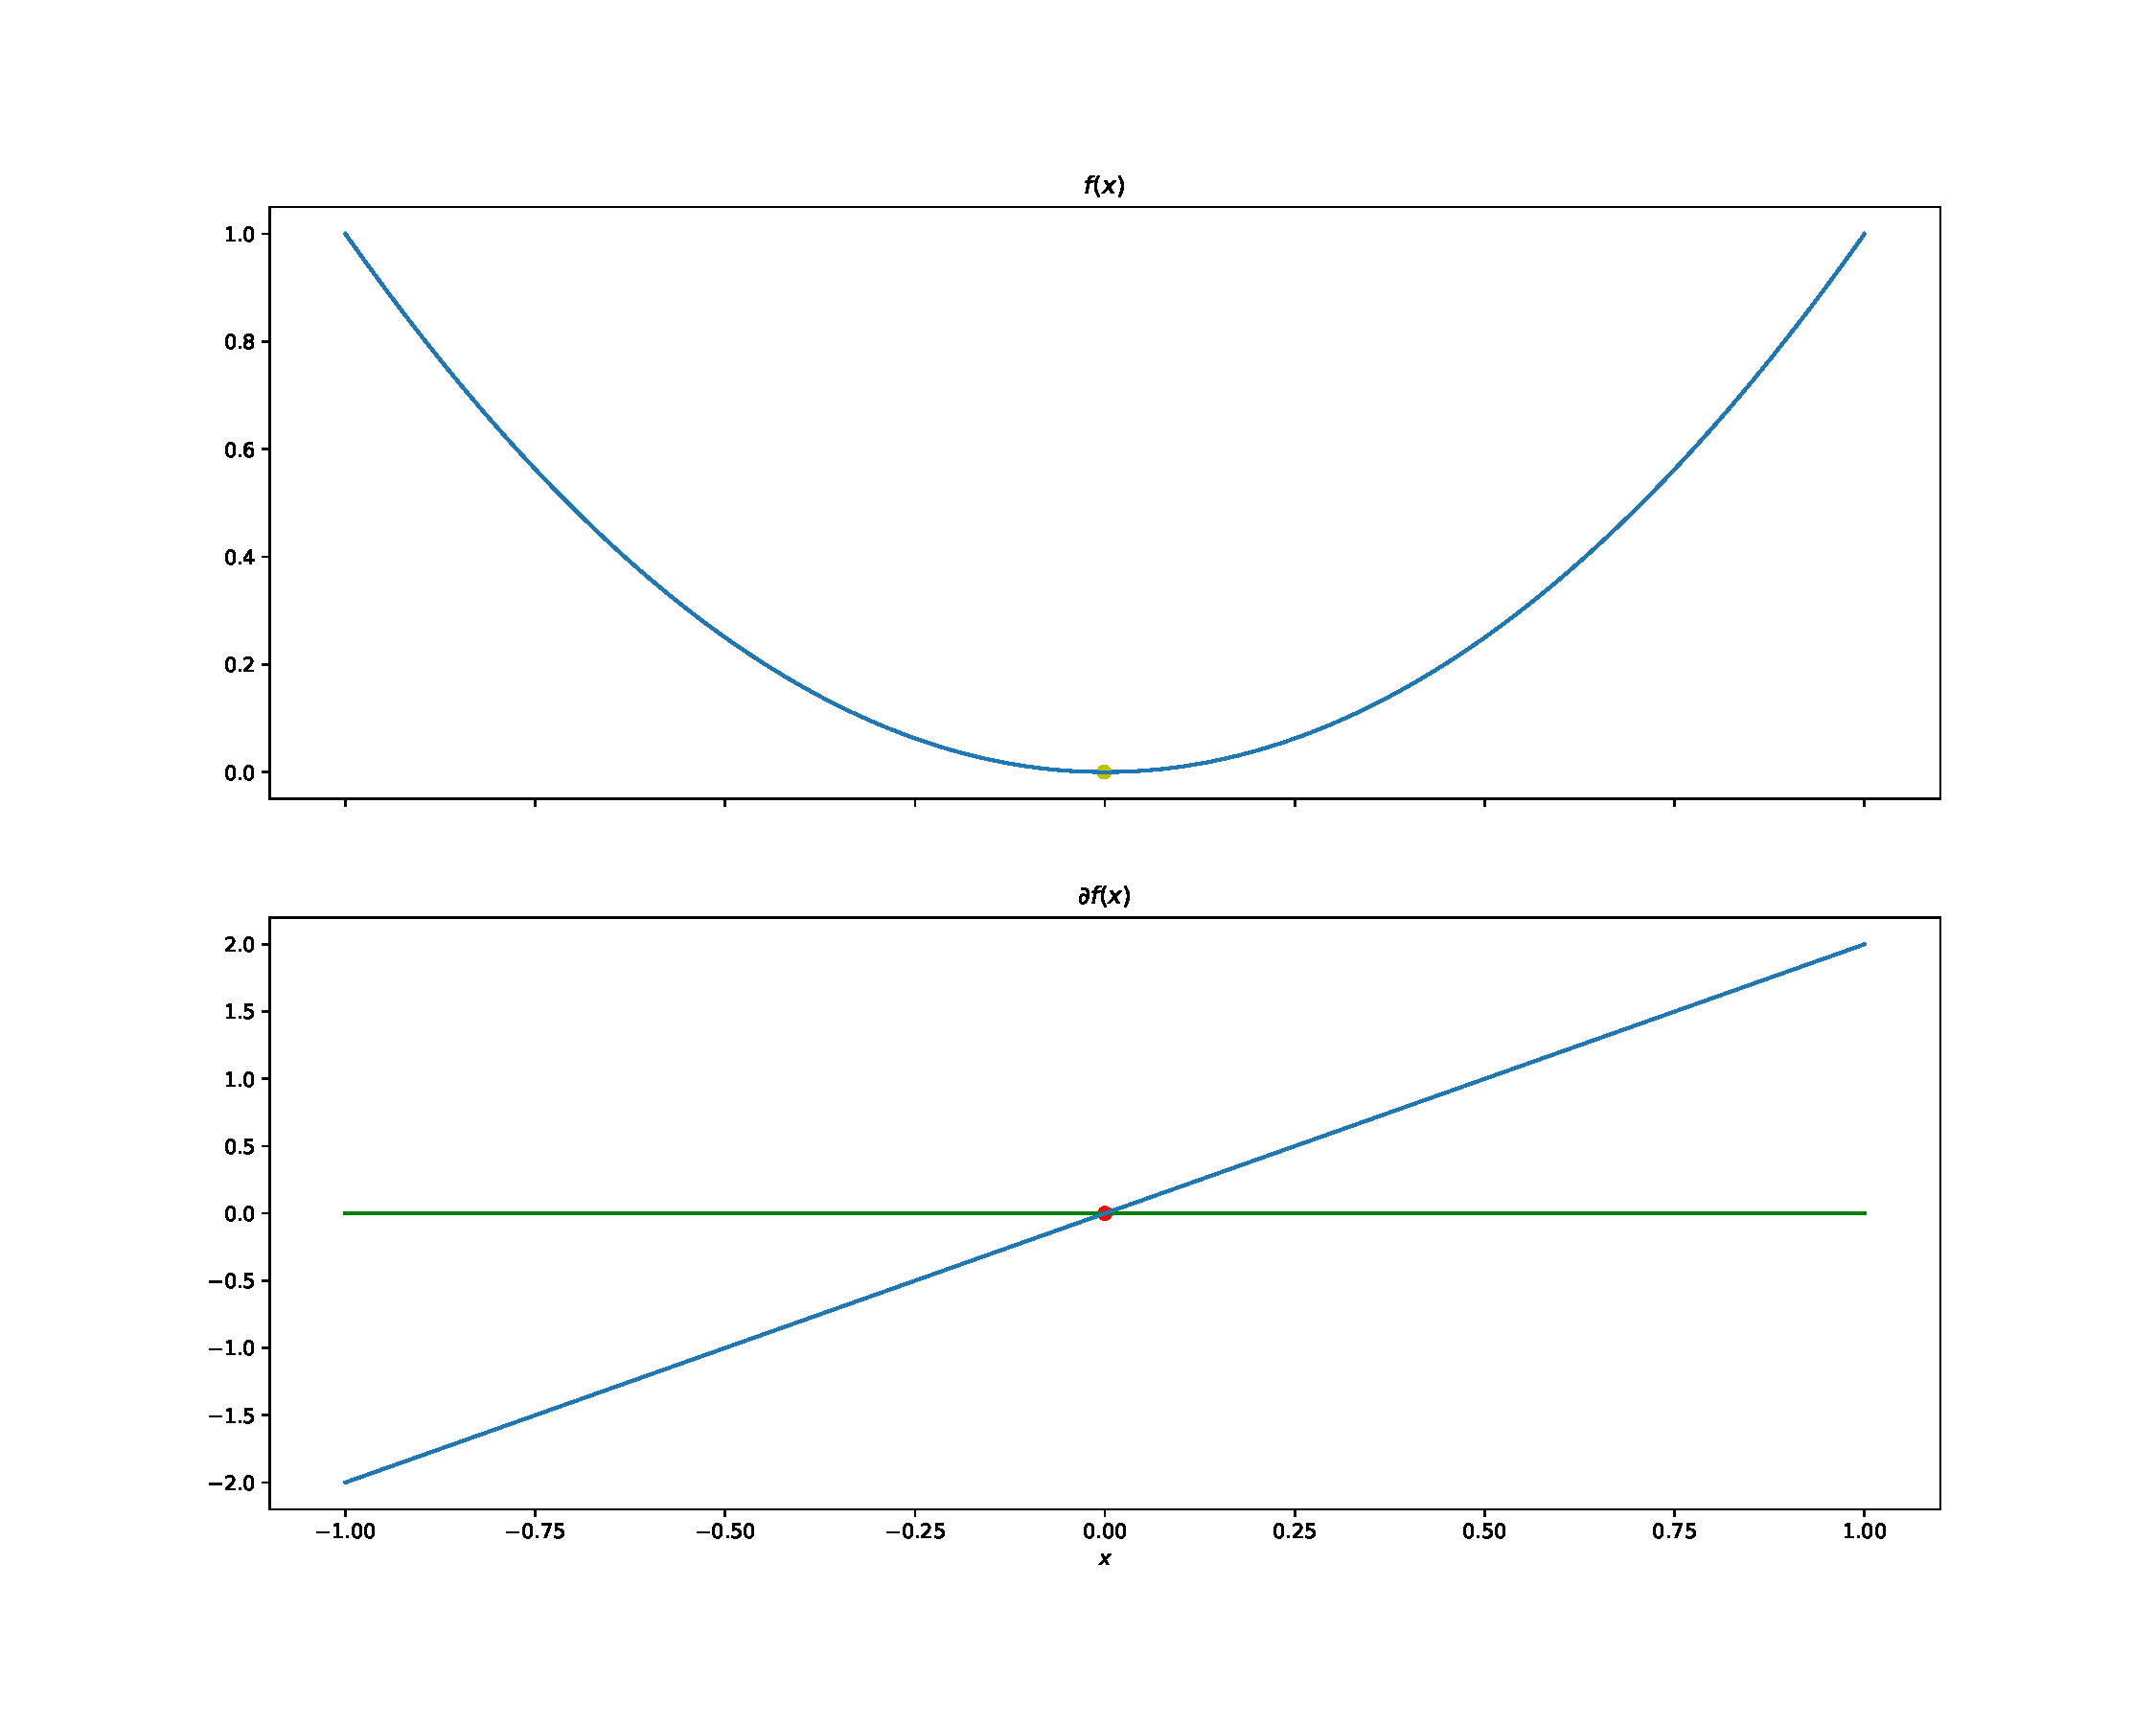
\includegraphics[width=\textwidth]{Chapter4/NeuroCom2021/ejemplo1_mse.pdf}
    \caption{Squared value function (top) and its corresponding subgradient (bottom). The green line represents the $0$ constant function. The yellow dot indicates the point minimizing the function.}
    \label{fig:sq_loss}
\end{figure}
This is the simplest case, since the squared function,
$f(x) = x^2 ,$
is differentiable, and its derivative is 
$\nabla f(x) = 2x$; both are shown in Figure~\ref{fig:sq_loss}.
Using the formulation of~\eqref{eq:subproblem_lambda}, the training error corresponding to the squared loss is
\begin{equation}
    \label{eq:opt_sq}
    \argmin_{\lambda \in [0, 1]} \mathcal{J}(\lambda) = \sum_{i=1}^{\npertask} \left({\lambda c_i + d_i}\right)^2 .
\end{equation}
In this case, $\mathcal{J}(\lambda)$ is a differentiable function, and its gradient is 
\begin{equation}
    \nonumber
    \mathcal{J}'(\lambda) = \sum_{i=1}^\npertask 2 c_i (\lambda c_i + d_i) .
\end{equation}
Solving $\mathcal{J}'(\lambda)= 0$ results in
%
\begin{equation*}
\lambda' =  -\frac{\sum_{i=1}^{\npertask} d_i c_i }{\sum_{i=1}^{\npertask} (c_i)^2 } ,
\end{equation*}
and the optimum is hence $\lambda^* = \max(0, \min(1, \lambda'))$.
\begin{figure}[t!]
    \centering
    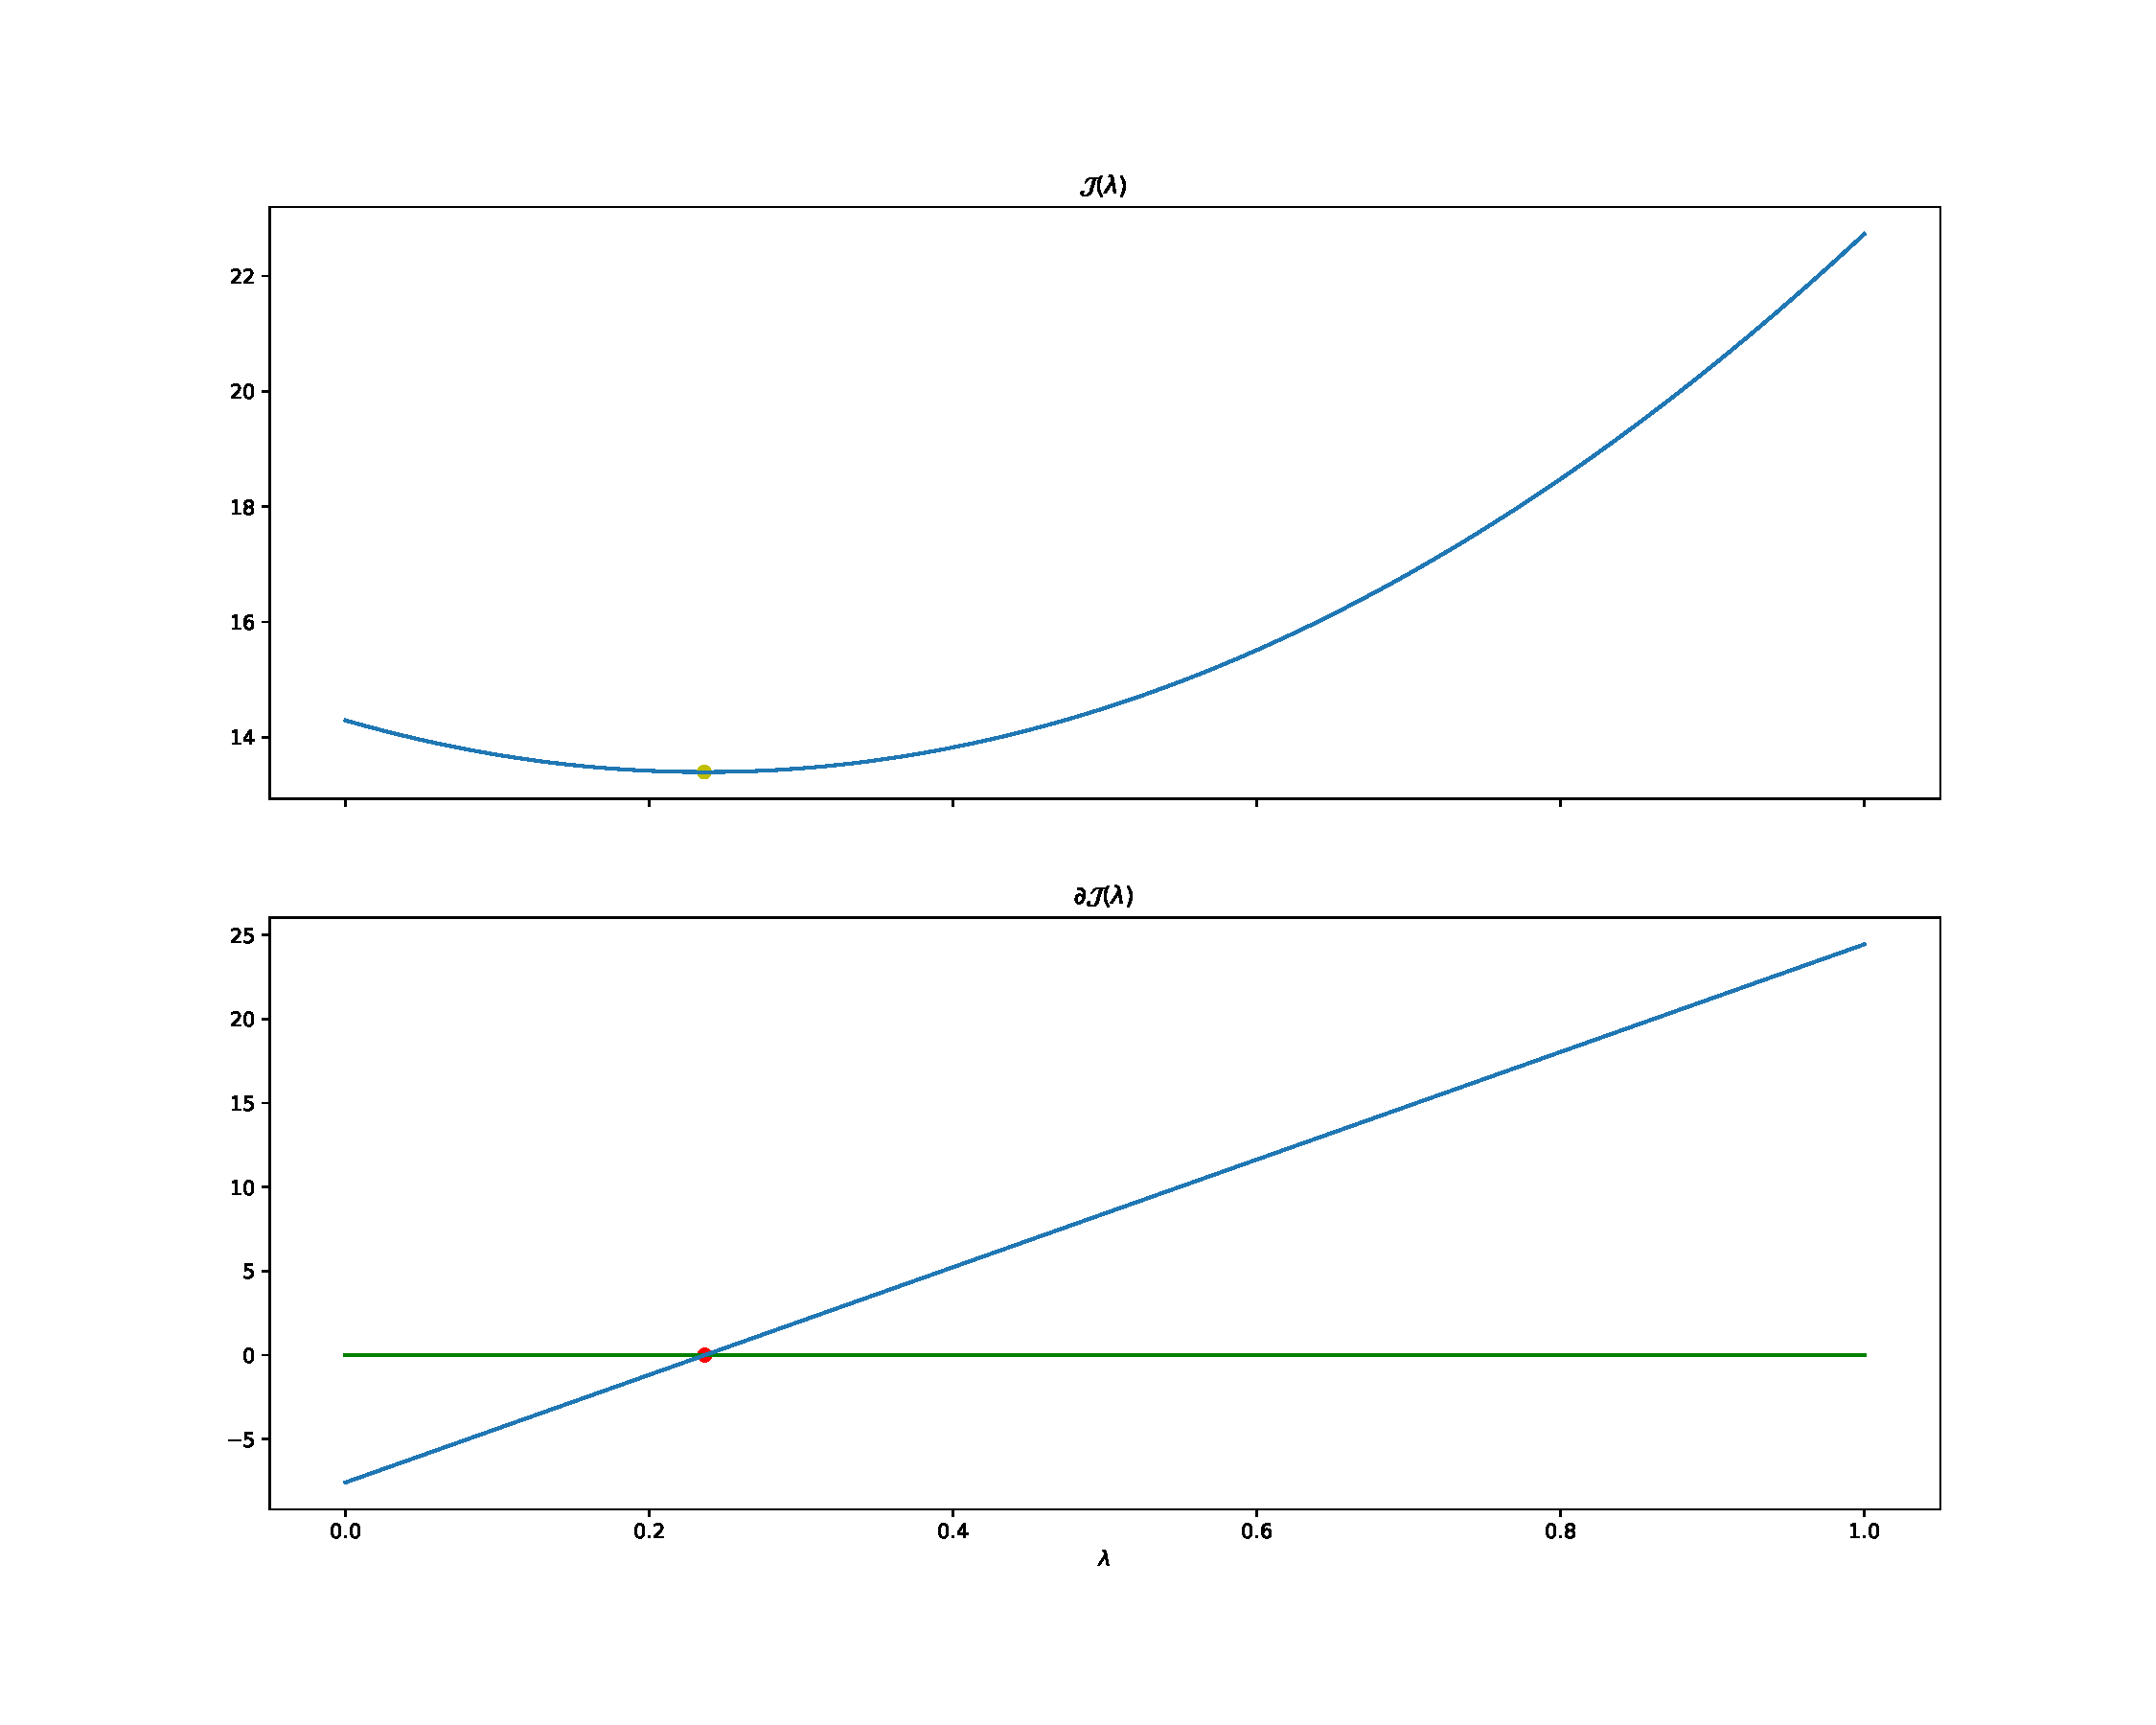
\includegraphics[width=\textwidth]{Chapter4/NeuroCom2021/ejemplo2_mse.pdf}
    \caption{Error using squared loss function (top) and its corresponding subgradient (bottom). The green line represents the $0$ constant function. The yellow dot is the point minimizing the error, and whose corresponding subgradient contains the value $0$.}
    \label{fig:sq_error}
\end{figure}

In Figure~\ref{fig:sq_error} the error function using $10$ random pairs $(c_i, d_i)$ and its corresponding differential is shown.

\paragraph*{Absolute loss.\\}
\begin{figure}[t!]
    \centering
    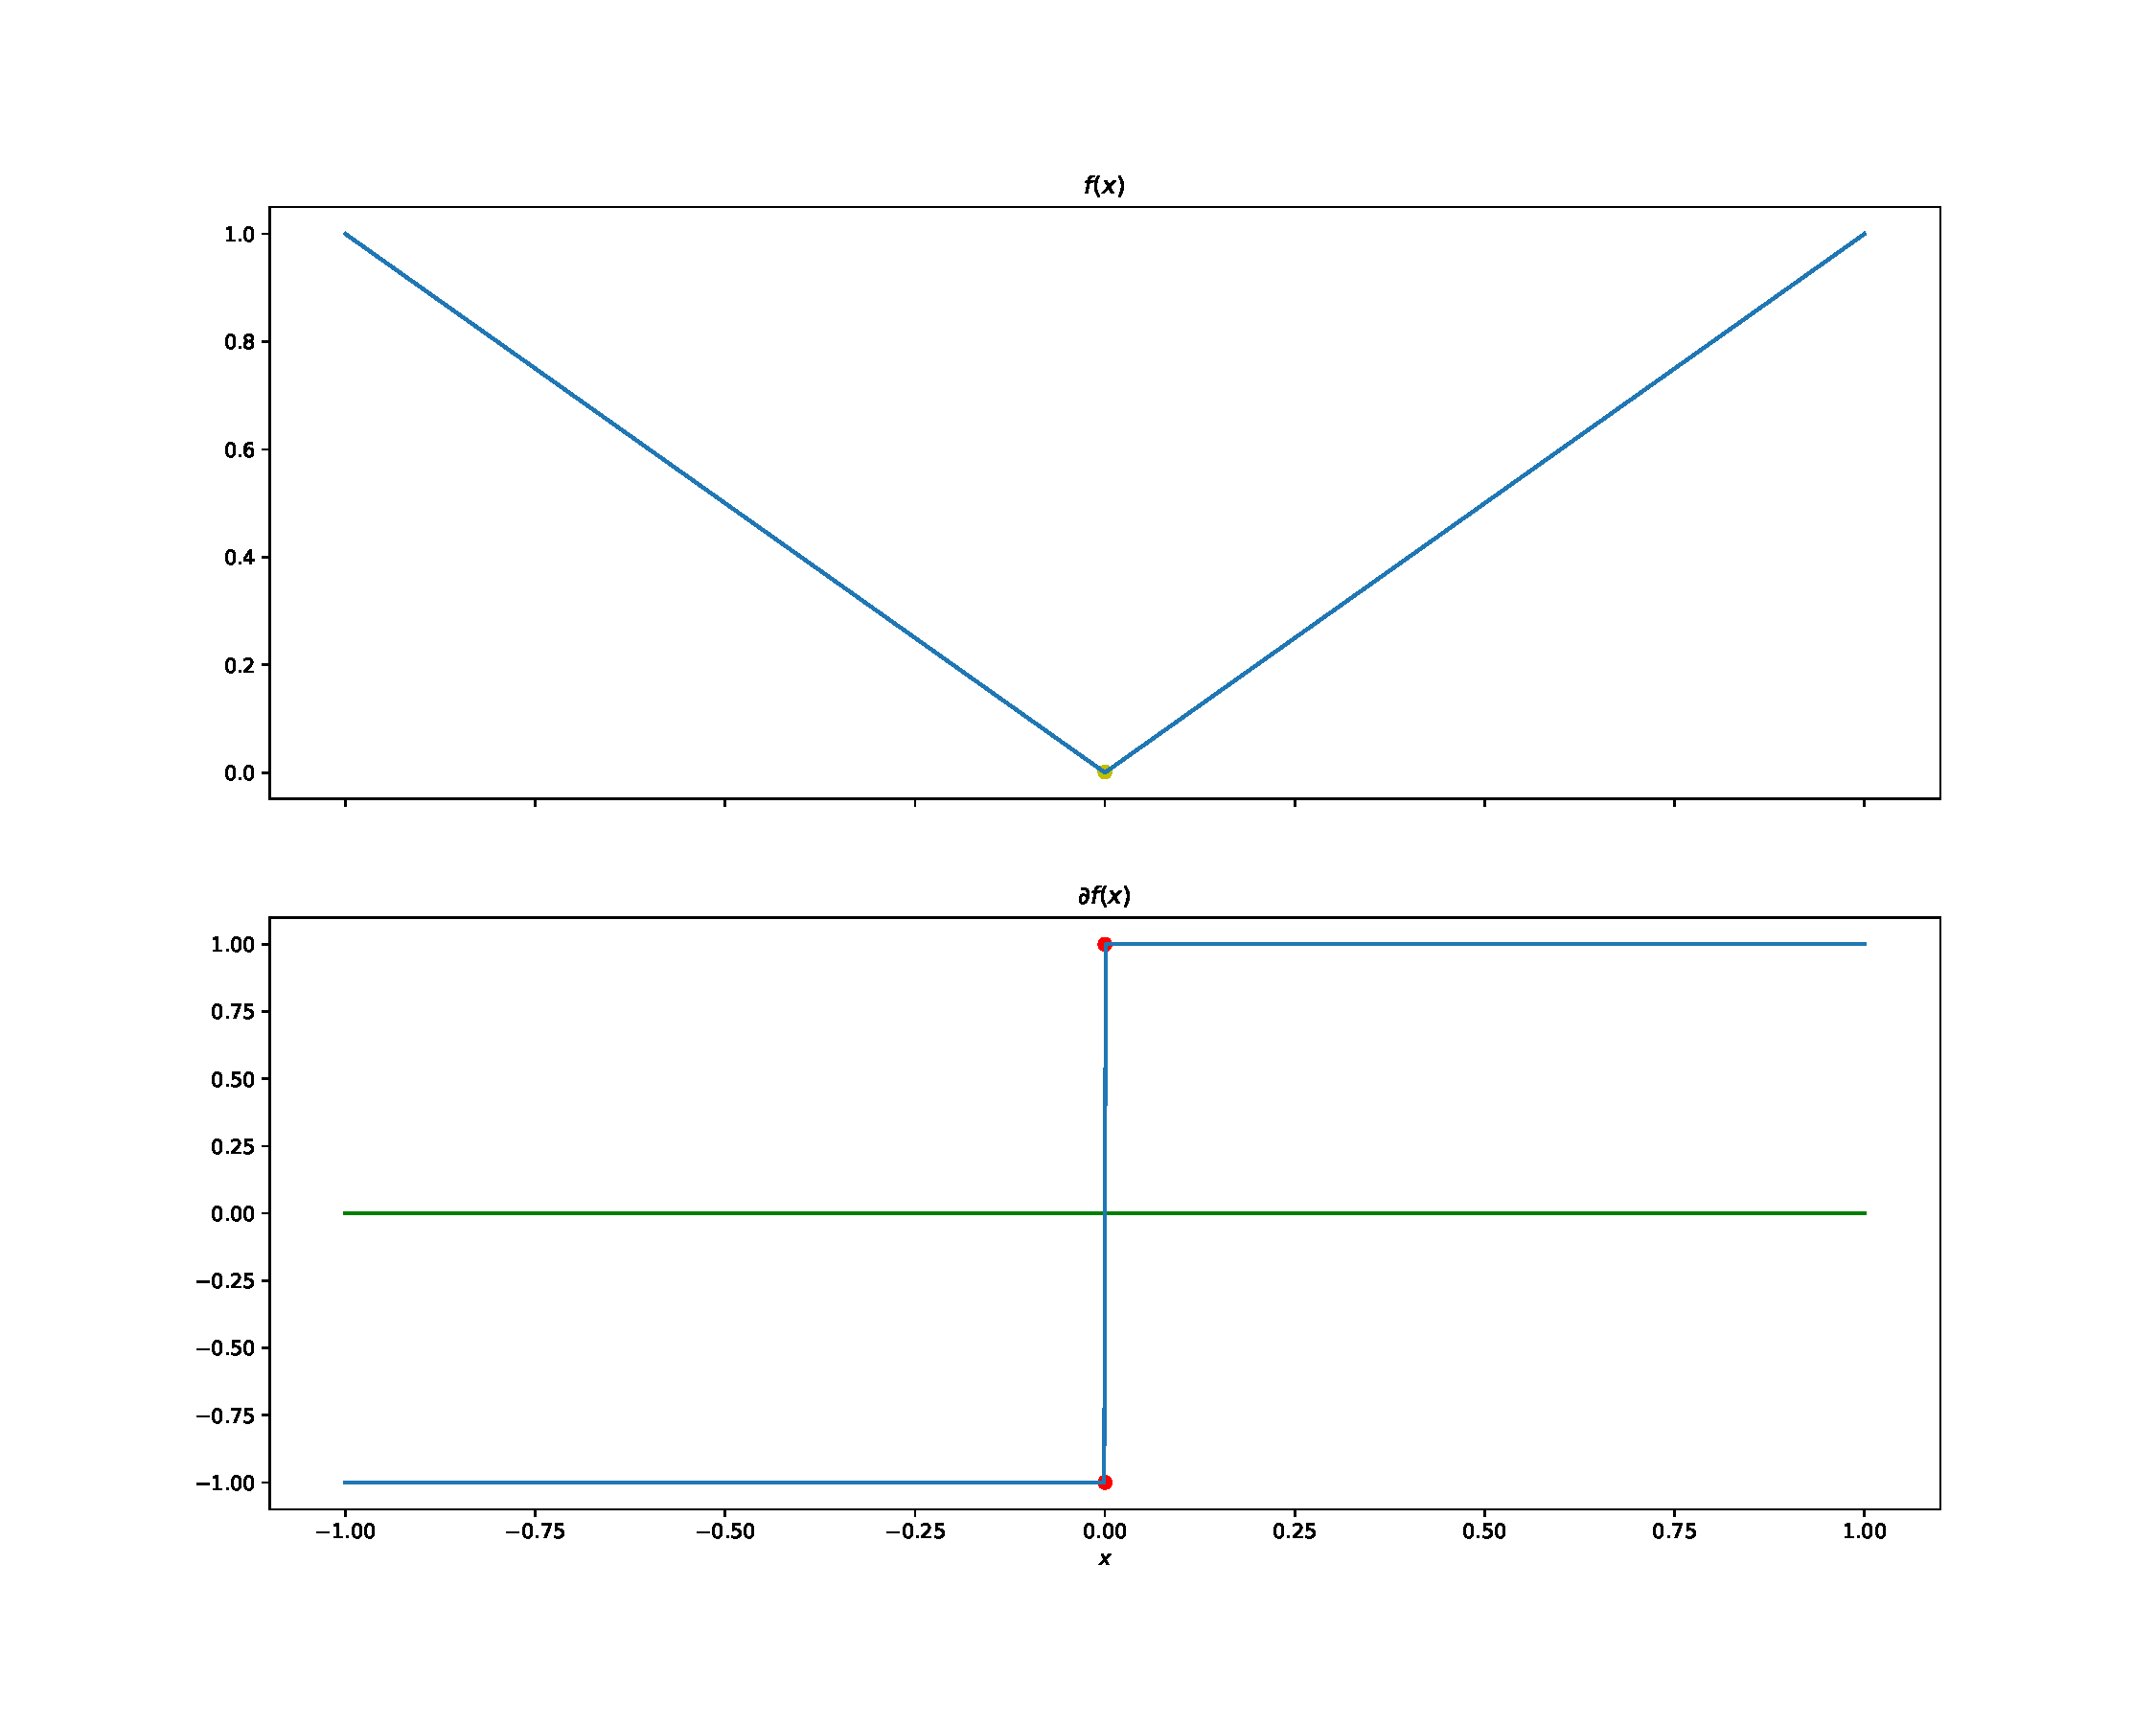
\includegraphics[width=\textwidth]{Chapter4/NeuroCom2021/ejemplo1_mae.pdf}
    \caption{Absolute value function (top) and its corresponding subgradient (bottom). The green line represents the $0$ constant function. The yellow dot indicates the point minimizing the function.}
    \label{fig:abs_loss}
\end{figure}
The absolute function 
\begin{equation}
    \nonumber
    f(x) = 
    \begin{cases}
    -x & x \leq 0, \\
    x & x > 0    
    \end{cases}
\end{equation}
is not differentiable at $0$, but the subgradient can be expressed at any point as
\begin{equation}
    \nonumber
    f(x) = 
    \begin{cases}
    -1 & x < 0, \\
    [-1, 1] & x = 0 , \\
    1 & x > 0 
    \end{cases},
\end{equation}
which is illustrated in Figure~\ref{fig:abs_loss}.
Using the formulation of~\eqref{eq:subproblem_lambda}, the training error corresponding to the absolute value loss is
\begin{equation}
    \label{eq:opt_abs}
    \argmin_{\lambda \in [0, 1]} \mathcal{J}(\lambda) = \sum_{i=1}^{\npertask} \abs{\lambda c_i + d_i}.
\end{equation}
Observe that in each term of the sum the subdifferential is 
\begin{align*}
    \partial \abs{\lambda c_i + d_i} = 
    \begin{cases}
        -\abs{c_i} &, \lambda c_i + d_i  < 0 \\
        [-\abs{c_i}, \abs{c_i}] &, \lambda c_i + d_i  = 0 \\
        \abs{c_i} &, \lambda c_i + d_i  > 0 \\
    \end{cases} 
\end{align*}
The elbows are obtained using the values $\frac{-d_i}{c_i}$, that can be clipped and sorted to get ${\lambda}_{(1)} < \ldots < {\lambda}_{(m)}$.
In~\citet[Proposition 2]{RuizAD21} we present a result to get the optimal $\lambda^*$.
\begin{prop}[Optimal $\lambda^*$ with absolute value loss]\label{prop:abs_neurocom2020}
    In problem~\eqref{eq:opt_abs} $\lambda^*=0$ is optimal iff
    \begin{equation}\nonumber
        - \sum_{j: \lambda_{(j)} < 0} \abs{c_{j}} + \sum_{j: \lambda_{(j)} > 0} \abs{c_{j}} < 0.
        \end{equation}
    If this condition does not hold, $\lambda^* \in (0,1)$ is optimal iff $\lambda^*$ is a feasible elbow, that is, $0 \leq \lambda^* = \lambda_{(k)} \leq 1$ for some $k=1, \dotsc, \npertask$, and
    \begin{equation}\label{sol_abs_e}
    - \sum_{j: \lambda_{(j)} < \lambda_{(k)}} \abs{c_{j}} + \sum_{j: \lambda_{(j)} > \lambda_{(k)}} \abs{c_{j}} \in \left[ -  \abs{c_{k}},  \abs{c_{k}}  \right] .
    \end{equation}
    If none of the previous conditions hold, then $\lambda^*=1$ is optimal.
\end{prop}
\begin{figure}[t!]
    \centering
    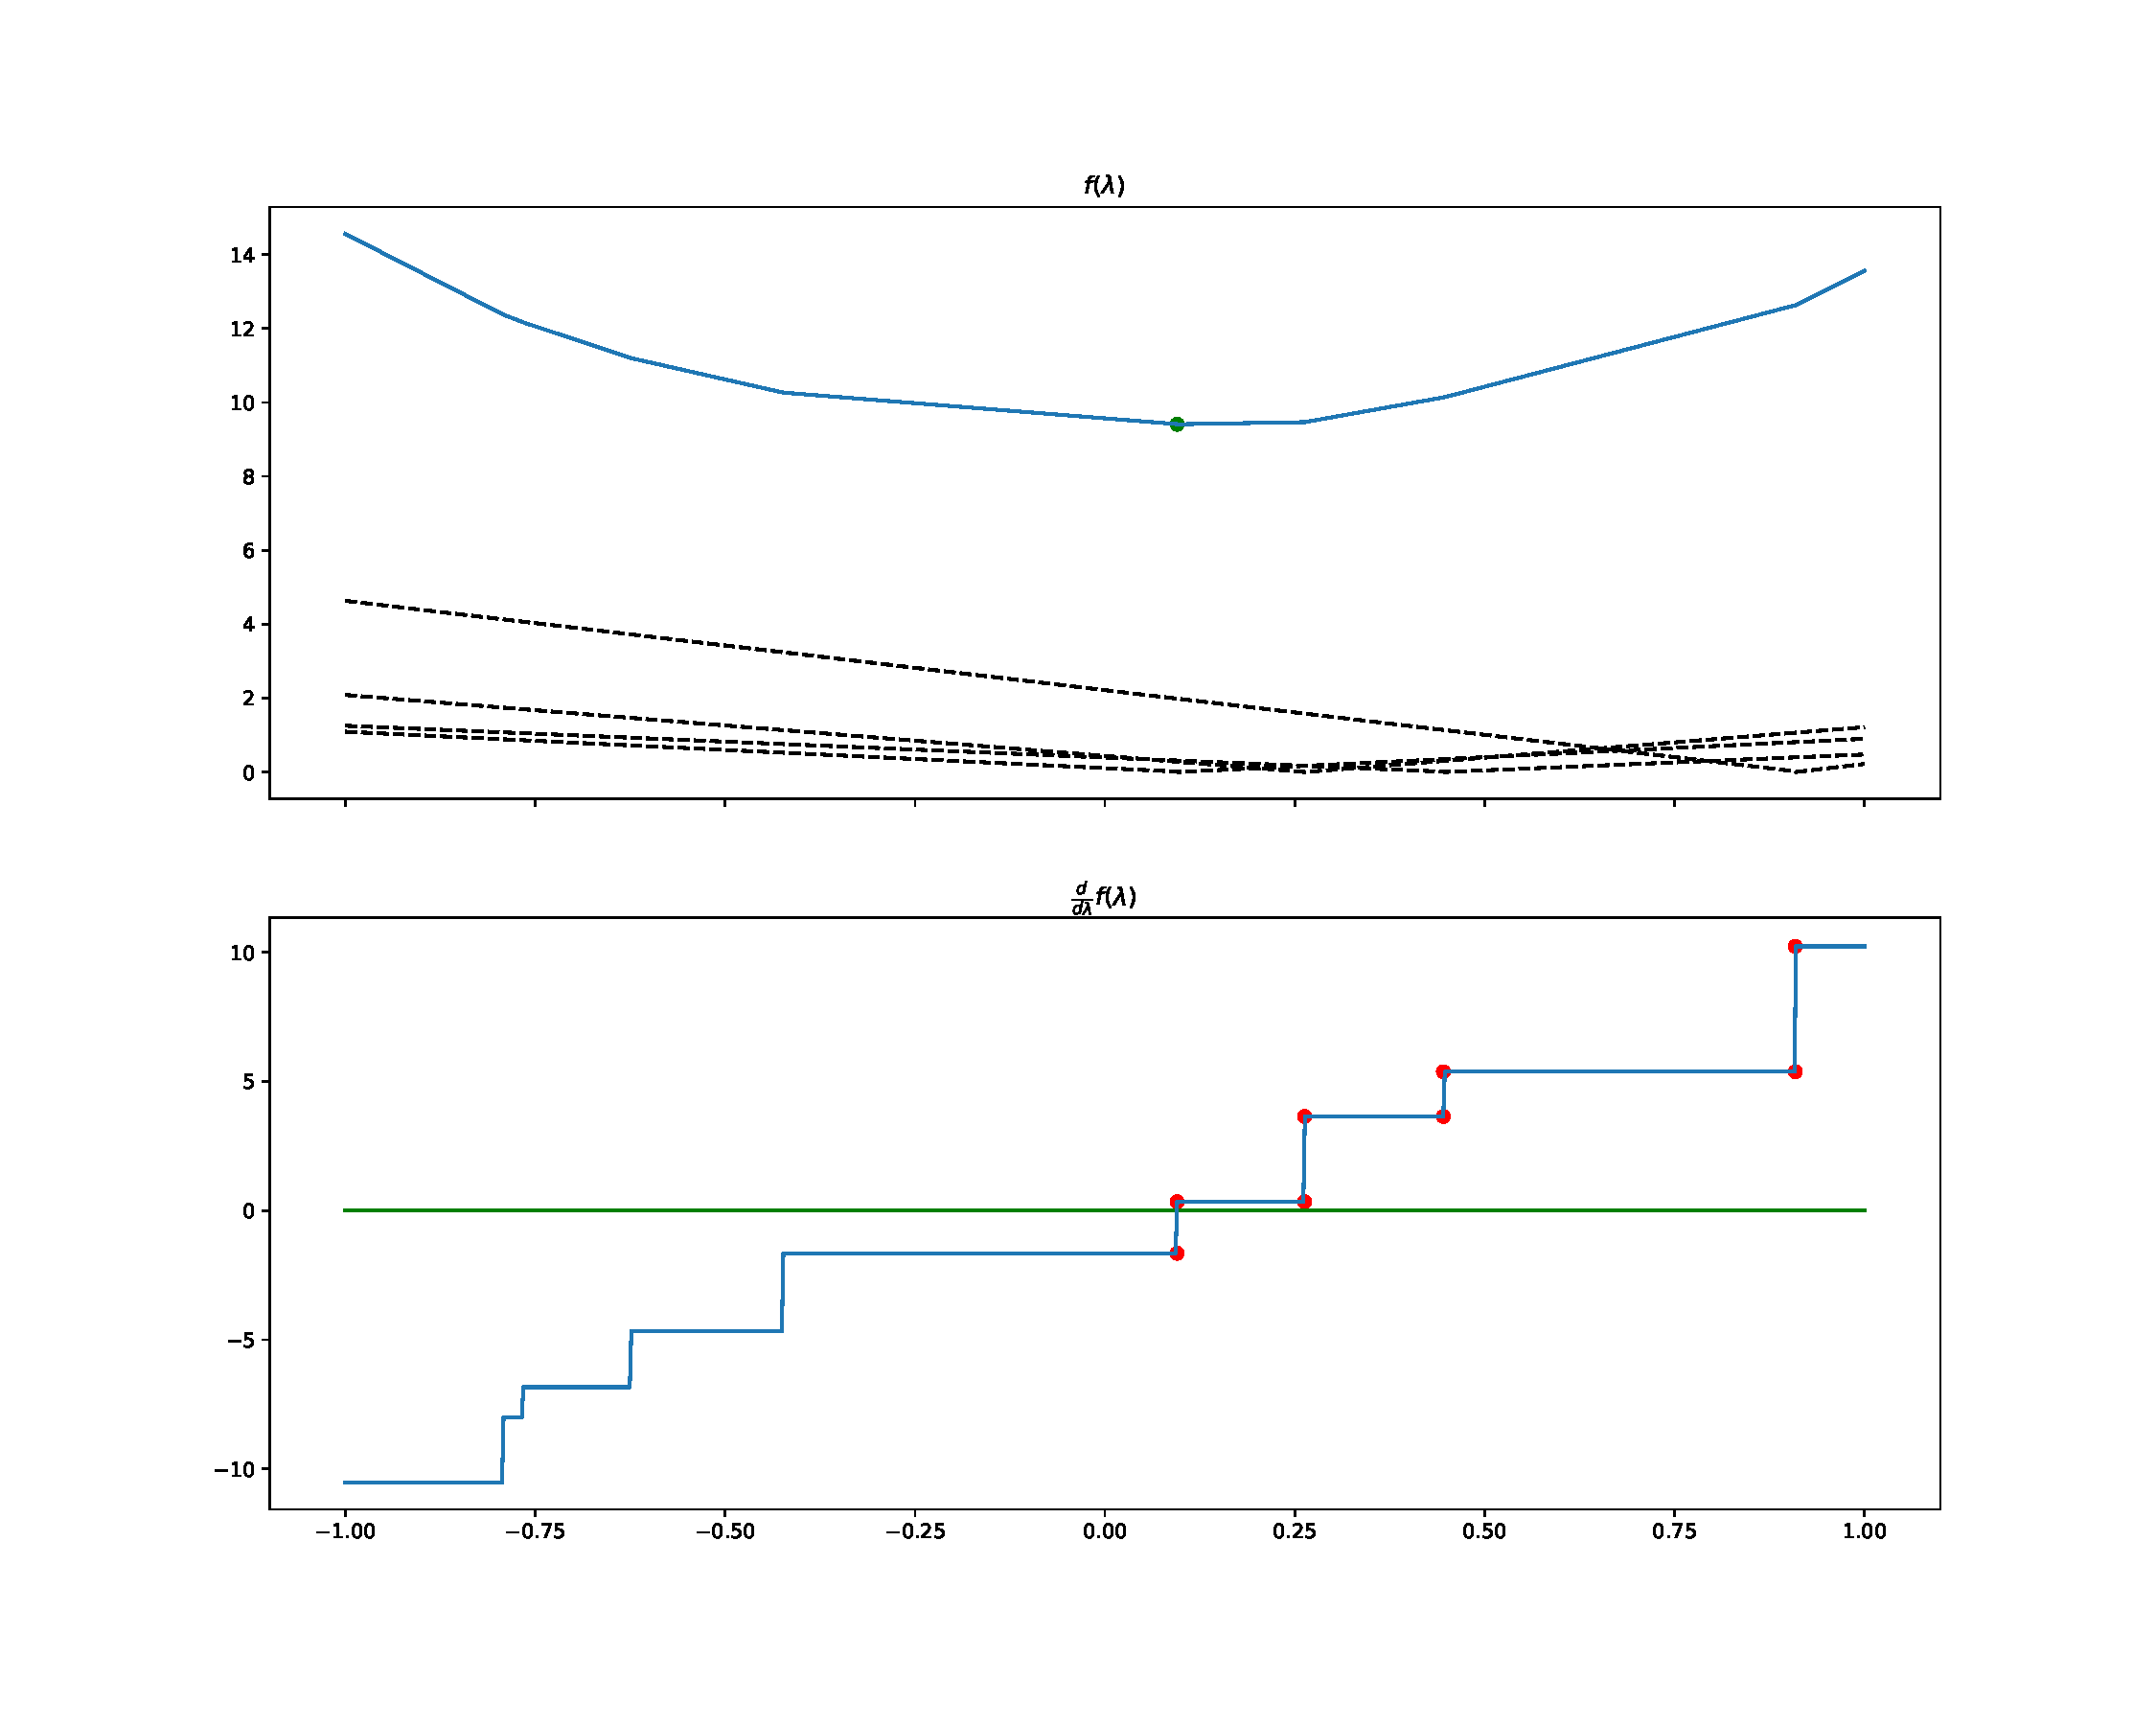
\includegraphics[width=\textwidth]{Chapter4/NeuroCom2021/ejemplo2_mae.pdf}
    \caption{Error using absolute loss function (top) and its corresponding subgradient (bottom). The green line represents the $0$ constant function. Red dots mark the extremes of the subdifferential intervals of non-differentiable points. The yellow dot is the point minimizing the error, and whose corresponding subgradient contains the value $0$.}
    \label{fig:abs_error}
\end{figure}
The result of this proposition is depicted in Figure~\ref{fig:abs_error}, where the error and its corresponding subgradient is computed for $10$ random pairs $(c_i, d_i)$.

\paragraph*{Hinge loss.\\}
The positive part function 
\begin{equation}
    \nonumber
    f(x) = 
    \begin{cases}
    0 & x \leq 0, \\
    x & x > 0    
    \end{cases}
\end{equation}
is not differentiable at $0$, but, again, the subgradient can be expressed at any point as
\begin{equation}
    \nonumber
    f(x) = 
    \begin{cases}
    0 & x < 0, \\
    [0, 1] & x = 0 , \\
    1 & x > 0 
    \end{cases},
\end{equation}
which is illustrated in Figure~\ref{fig:hinge_loss}.
\begin{figure}[t!]
    \centering
    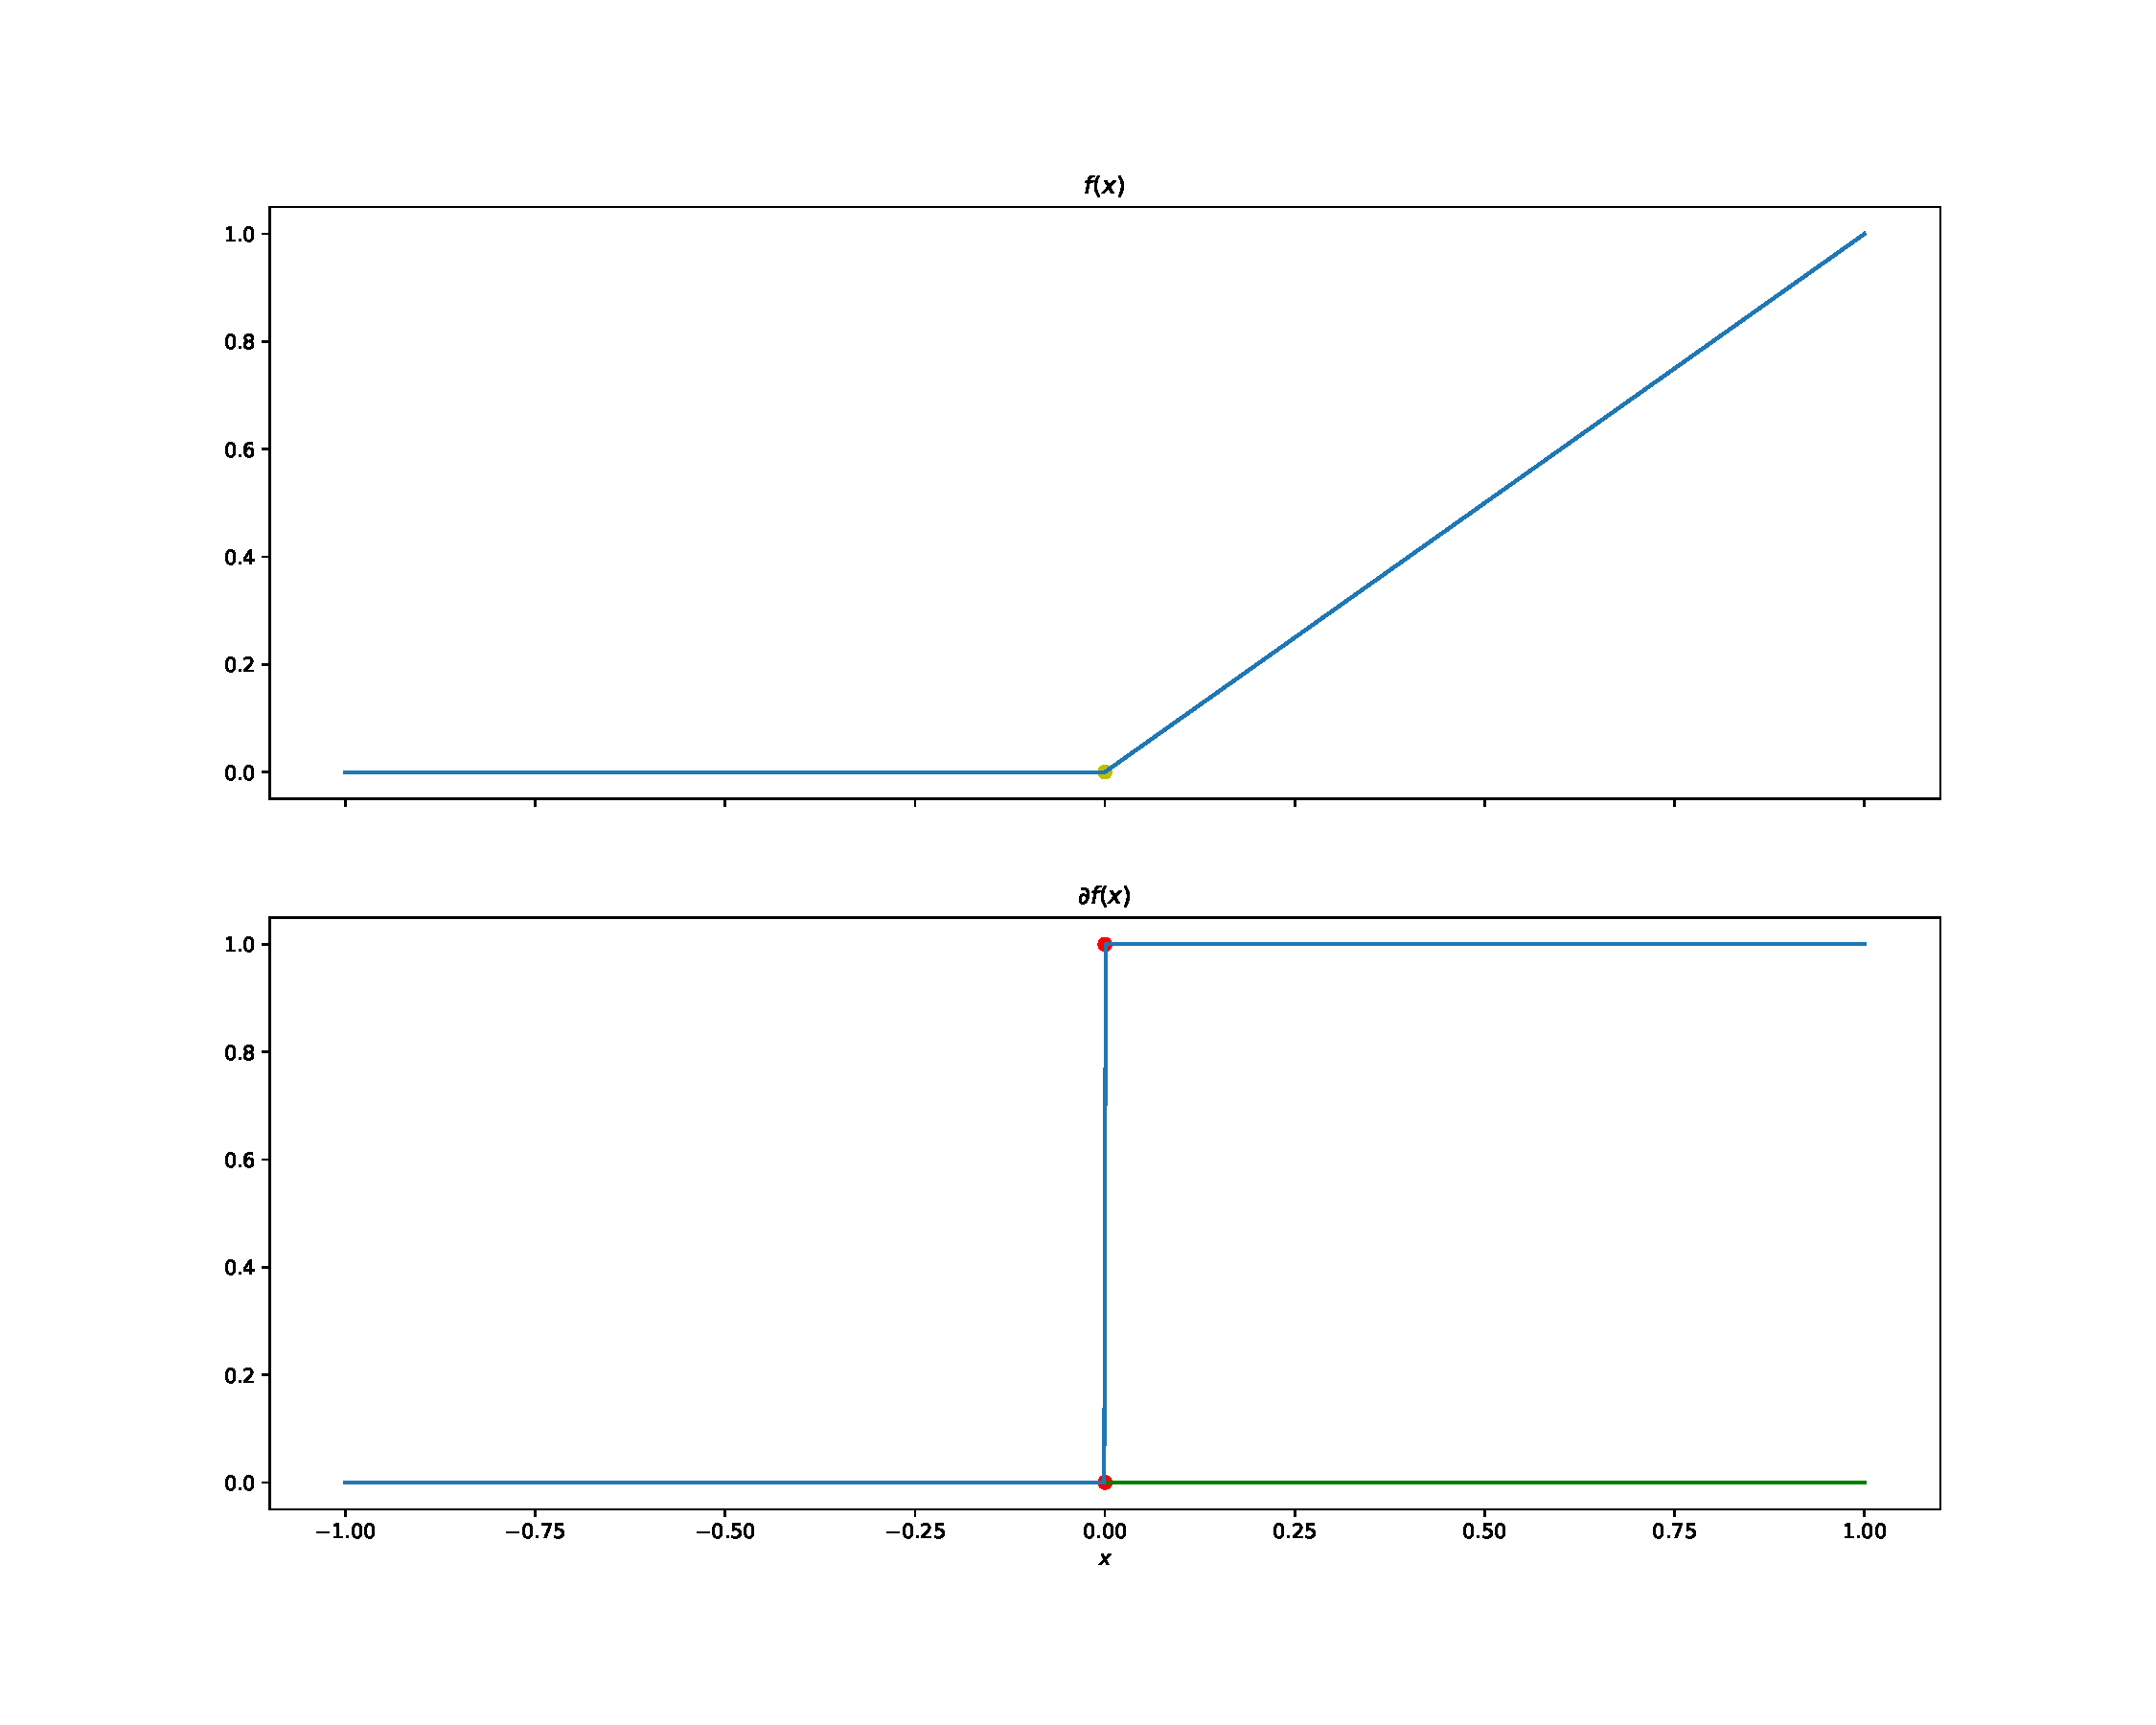
\includegraphics[width=\textwidth]{Chapter4/NeuroCom2021/ejemplo1_hinge.pdf}
    \caption{Positive part function (top) and its corresponding subgradient (bottom). The green line represents the $0$ constant function. The yellow dot indicates the point minimizing the function.}
    \label{fig:hinge_loss}
\end{figure}
Using the formulation of~\eqref{eq:subproblem_lambda}, the training error corresponding to the hinge loss is
\begin{equation}
    \label{eq:opt_hinge_l1}
    \argmin_{\lambda \in [0, 1]} \mathcal{J}(\lambda) = \sum_{i=1}^{\npertask} \pospart{\lambda c_i + d_i}.
\end{equation}
Observe that in each term of the sum the subdifferential is 
\begin{align*}
    \partial \left[\lambda c_i + d_i \right]_+ = 
    \begin{cases}
        0 &, \lambda c_i + d_i  < 0 \\
        [\min(0, c_i), \max(0, c_i)] &, \lambda c_i + d_i  = 0 \\
        c_i &, \lambda c_i + d_i  > 0 \\
    \end{cases} \; .
\end{align*}
That is, the elbows are related to the values $\frac{-d_i}{c_i}$, that can be clipped and sorted to obtain the elbows ${\lambda}_{(1)} < \ldots < {\lambda}_{(m)}$.
In~\citet[Proposition 2]{RuizAD21} we present a result to get the optimal $\lambda^*$.
\begin{prop}[Optimal $\lambda^*$ with hinge loss]\label{prop:hinge_neurocom2020}
    In~\eqref{eq:opt_hinge_l1}, $\lambda^*=0$ is optimal iff
    \begin{equation}\label{eq:sol_hinge_0}
        -\sum_{j: \lambda_{(j)}<0} \max(0, c_{(j)}) - \sum_{\lambda_{(j)}>0} \min(0, c_{(j)}) \leq 0 .
        \end{equation}
        If this condition does not hold, a value $\lambda^* \in (0, 1)$ is optimal for problem~\eqref{eq:opt_hinge_l1} iff $\lambda^* \in \set{0, 1}$ or $\lambda^*$ is a feasible elbow, that is, $0 \leq \lambda^* = \lambda_{(k)} \leq 1$ for some $k=1, \dotsc, \npertask$, and
    \begin{equation}\label{eq:sol_hinge}
        -\sum_{j: \lambda_{(j)}< \lambda_{(k)}} \max(0, c_{(j)}) - \sum_{j: \lambda_{(j)}>  \lambda_{(k)}} \min(0, c_{(j)}) \in \left[\min(0, c_{(k)}), \max(0, c_{(k)}) \right] .
    \end{equation}
    If none of the previous conditions hold, then $\lambda^*=1$ is optimal.
\end{prop}
\begin{figure}[t!]
    \centering
    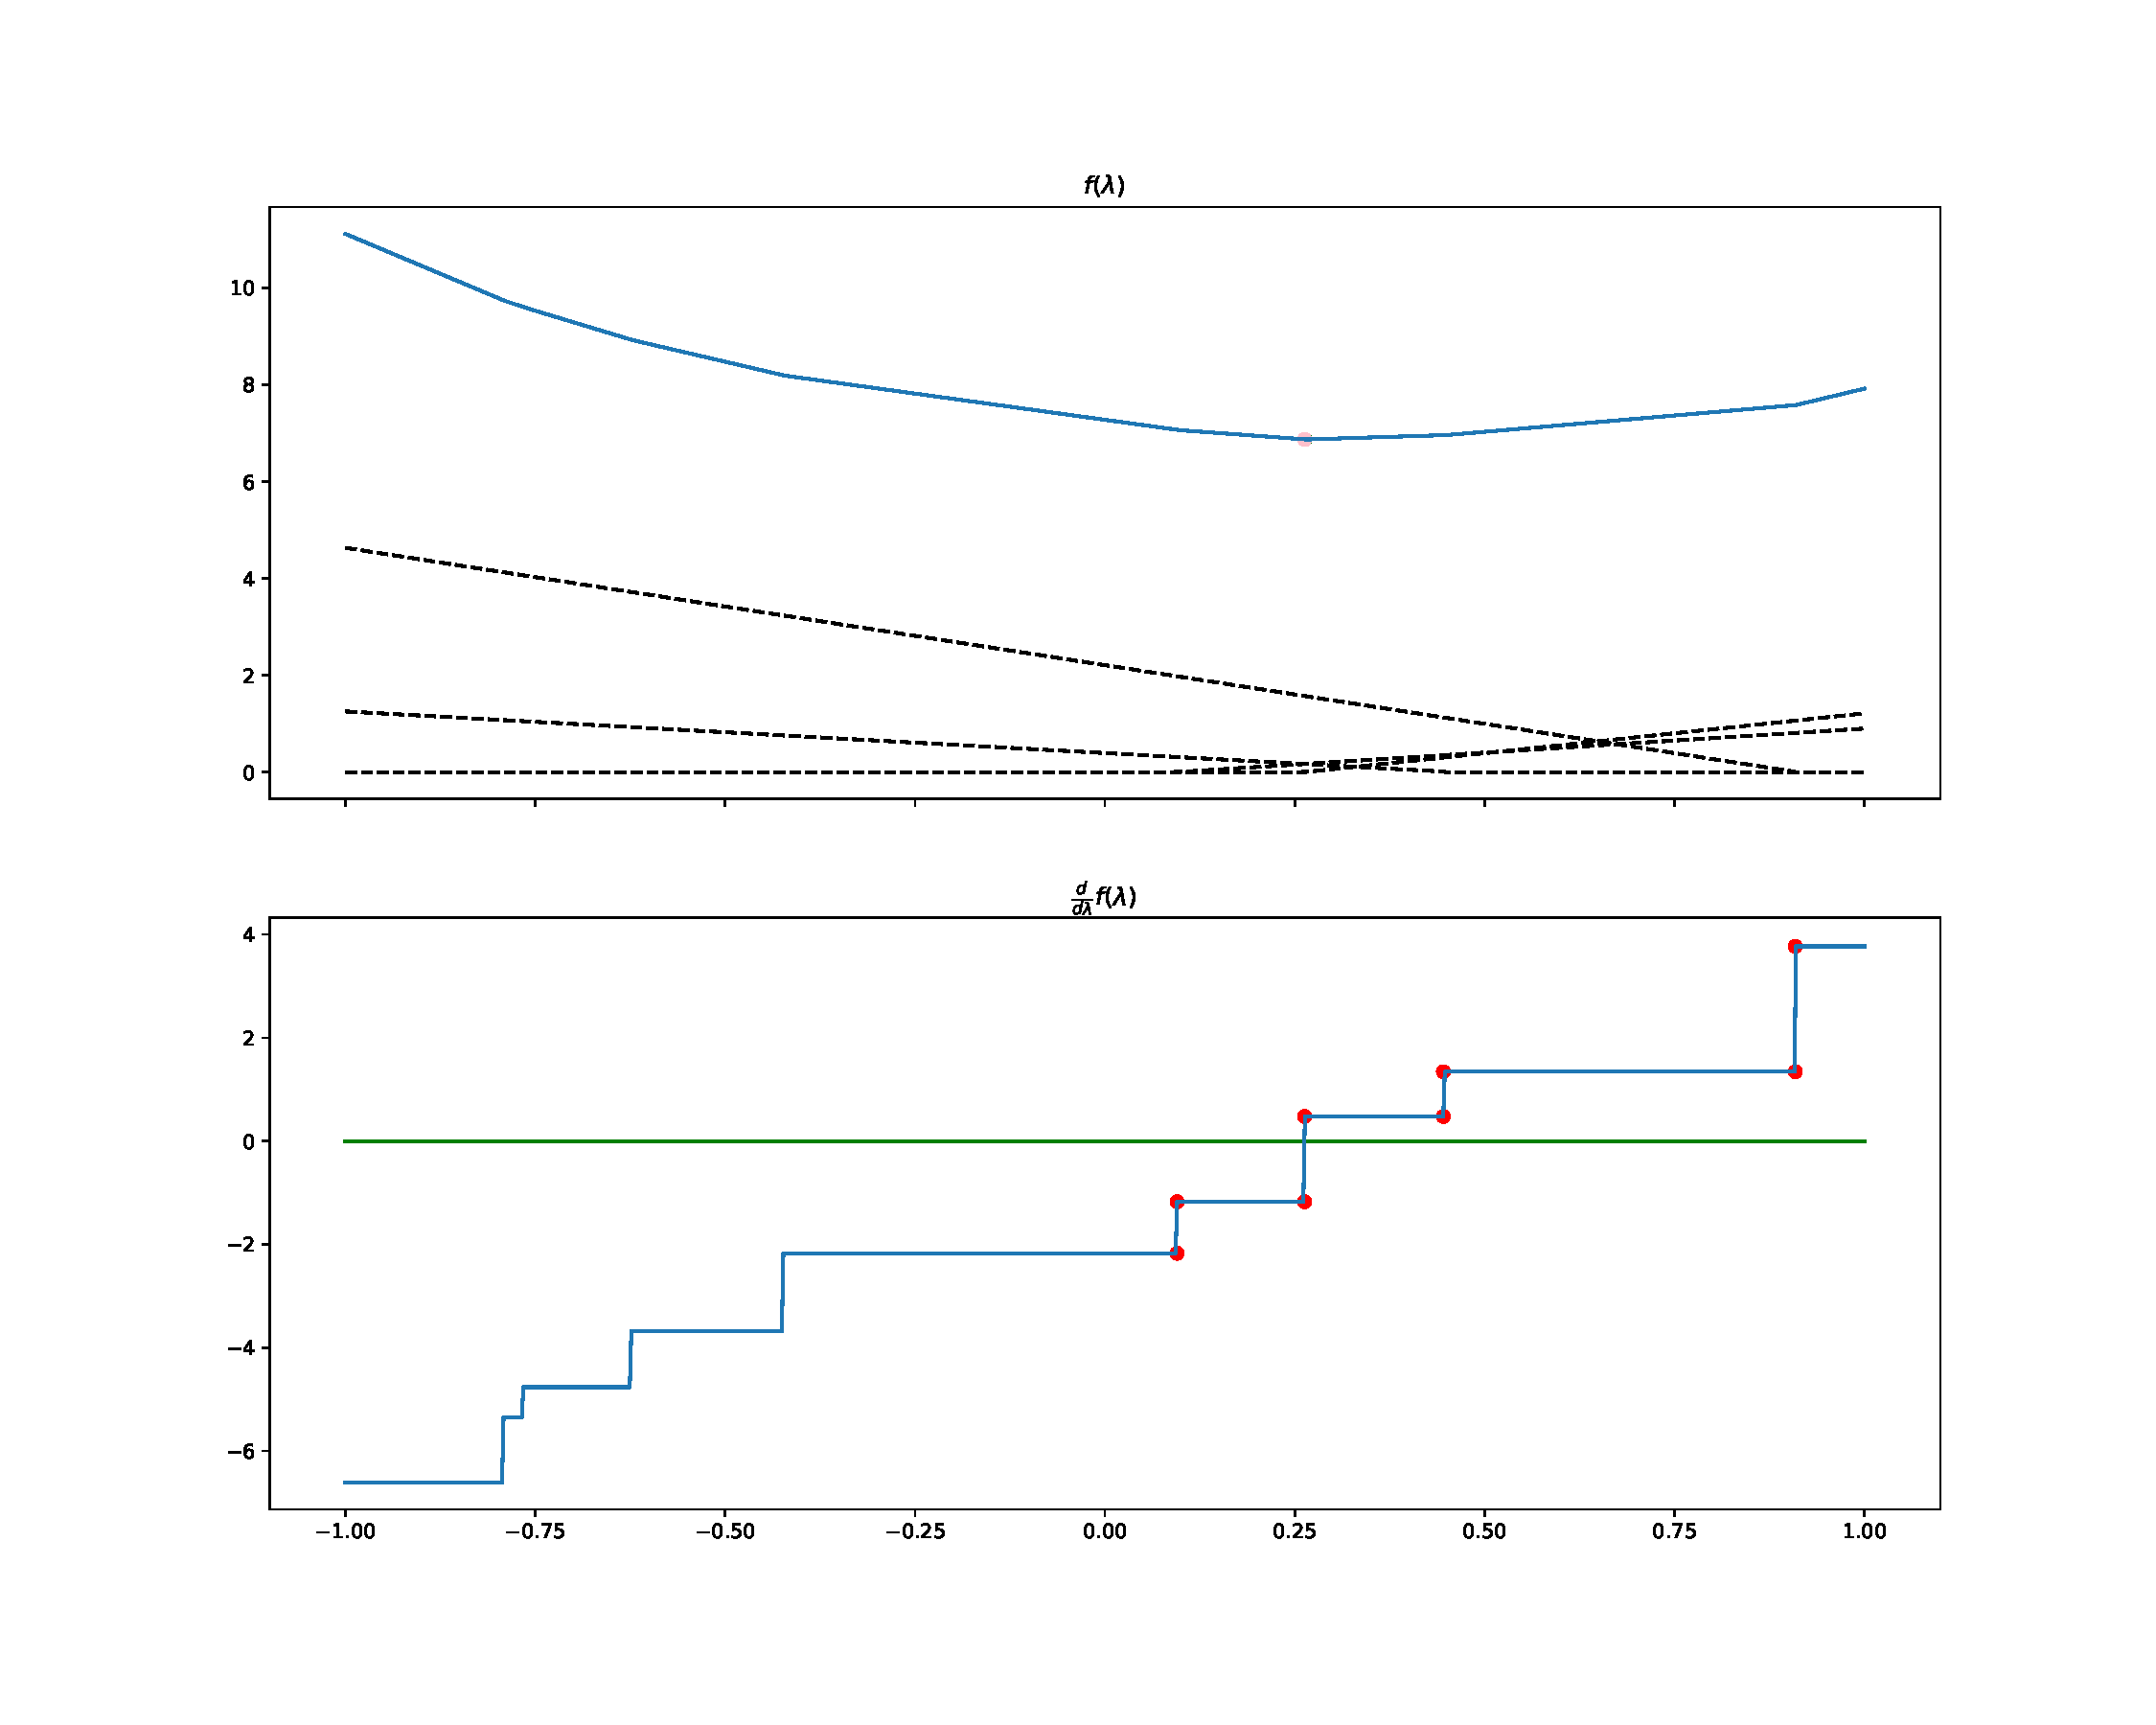
\includegraphics[width=\textwidth]{Chapter4/NeuroCom2021/ejemplo2_hinge.pdf}
    \caption{Error using hinge loss function (top) and its corresponding subgradient (bottom). The green line represents the $0$ constant function. Red dots mark the extremes of the subdifferential intervals of non-differentiable points. The yellow dot is the point minimizing the error, and whose corresponding subgradient contains the value $0$.}
    \label{fig:hinge_error}
\end{figure}

Again, the results of the proposition are illustrated in Figure~\ref{fig:hinge_error}, where $10$ pairs $(c_i, d_i)$ are randomly sampled, and the corresponding error function $\mathcal{J}(\lambda)$ and its subgradient are shown.

\paragraph*{Squared hinge loss.\\}
The squared positive part function is
\begin{equation}
    \nonumber
    f(x) = 
    \begin{cases}
    0 & x \leq 0, \\
    x^2 & x > 0    
    \end{cases}
\end{equation}
and its gradient can be expressed at any point as
\begin{equation}
    \nonumber
    f(x) = 
    \begin{cases}
    0 & x \leq 0, \\
    2x & x > 0 
    \end{cases},
\end{equation}
which is illustrated in Figure~\ref{fig:hinge_loss}.
Although the gradient can be defined at any point, the definition by parts makes it difficult to obtain results.
\begin{figure}[t!]
    \centering
    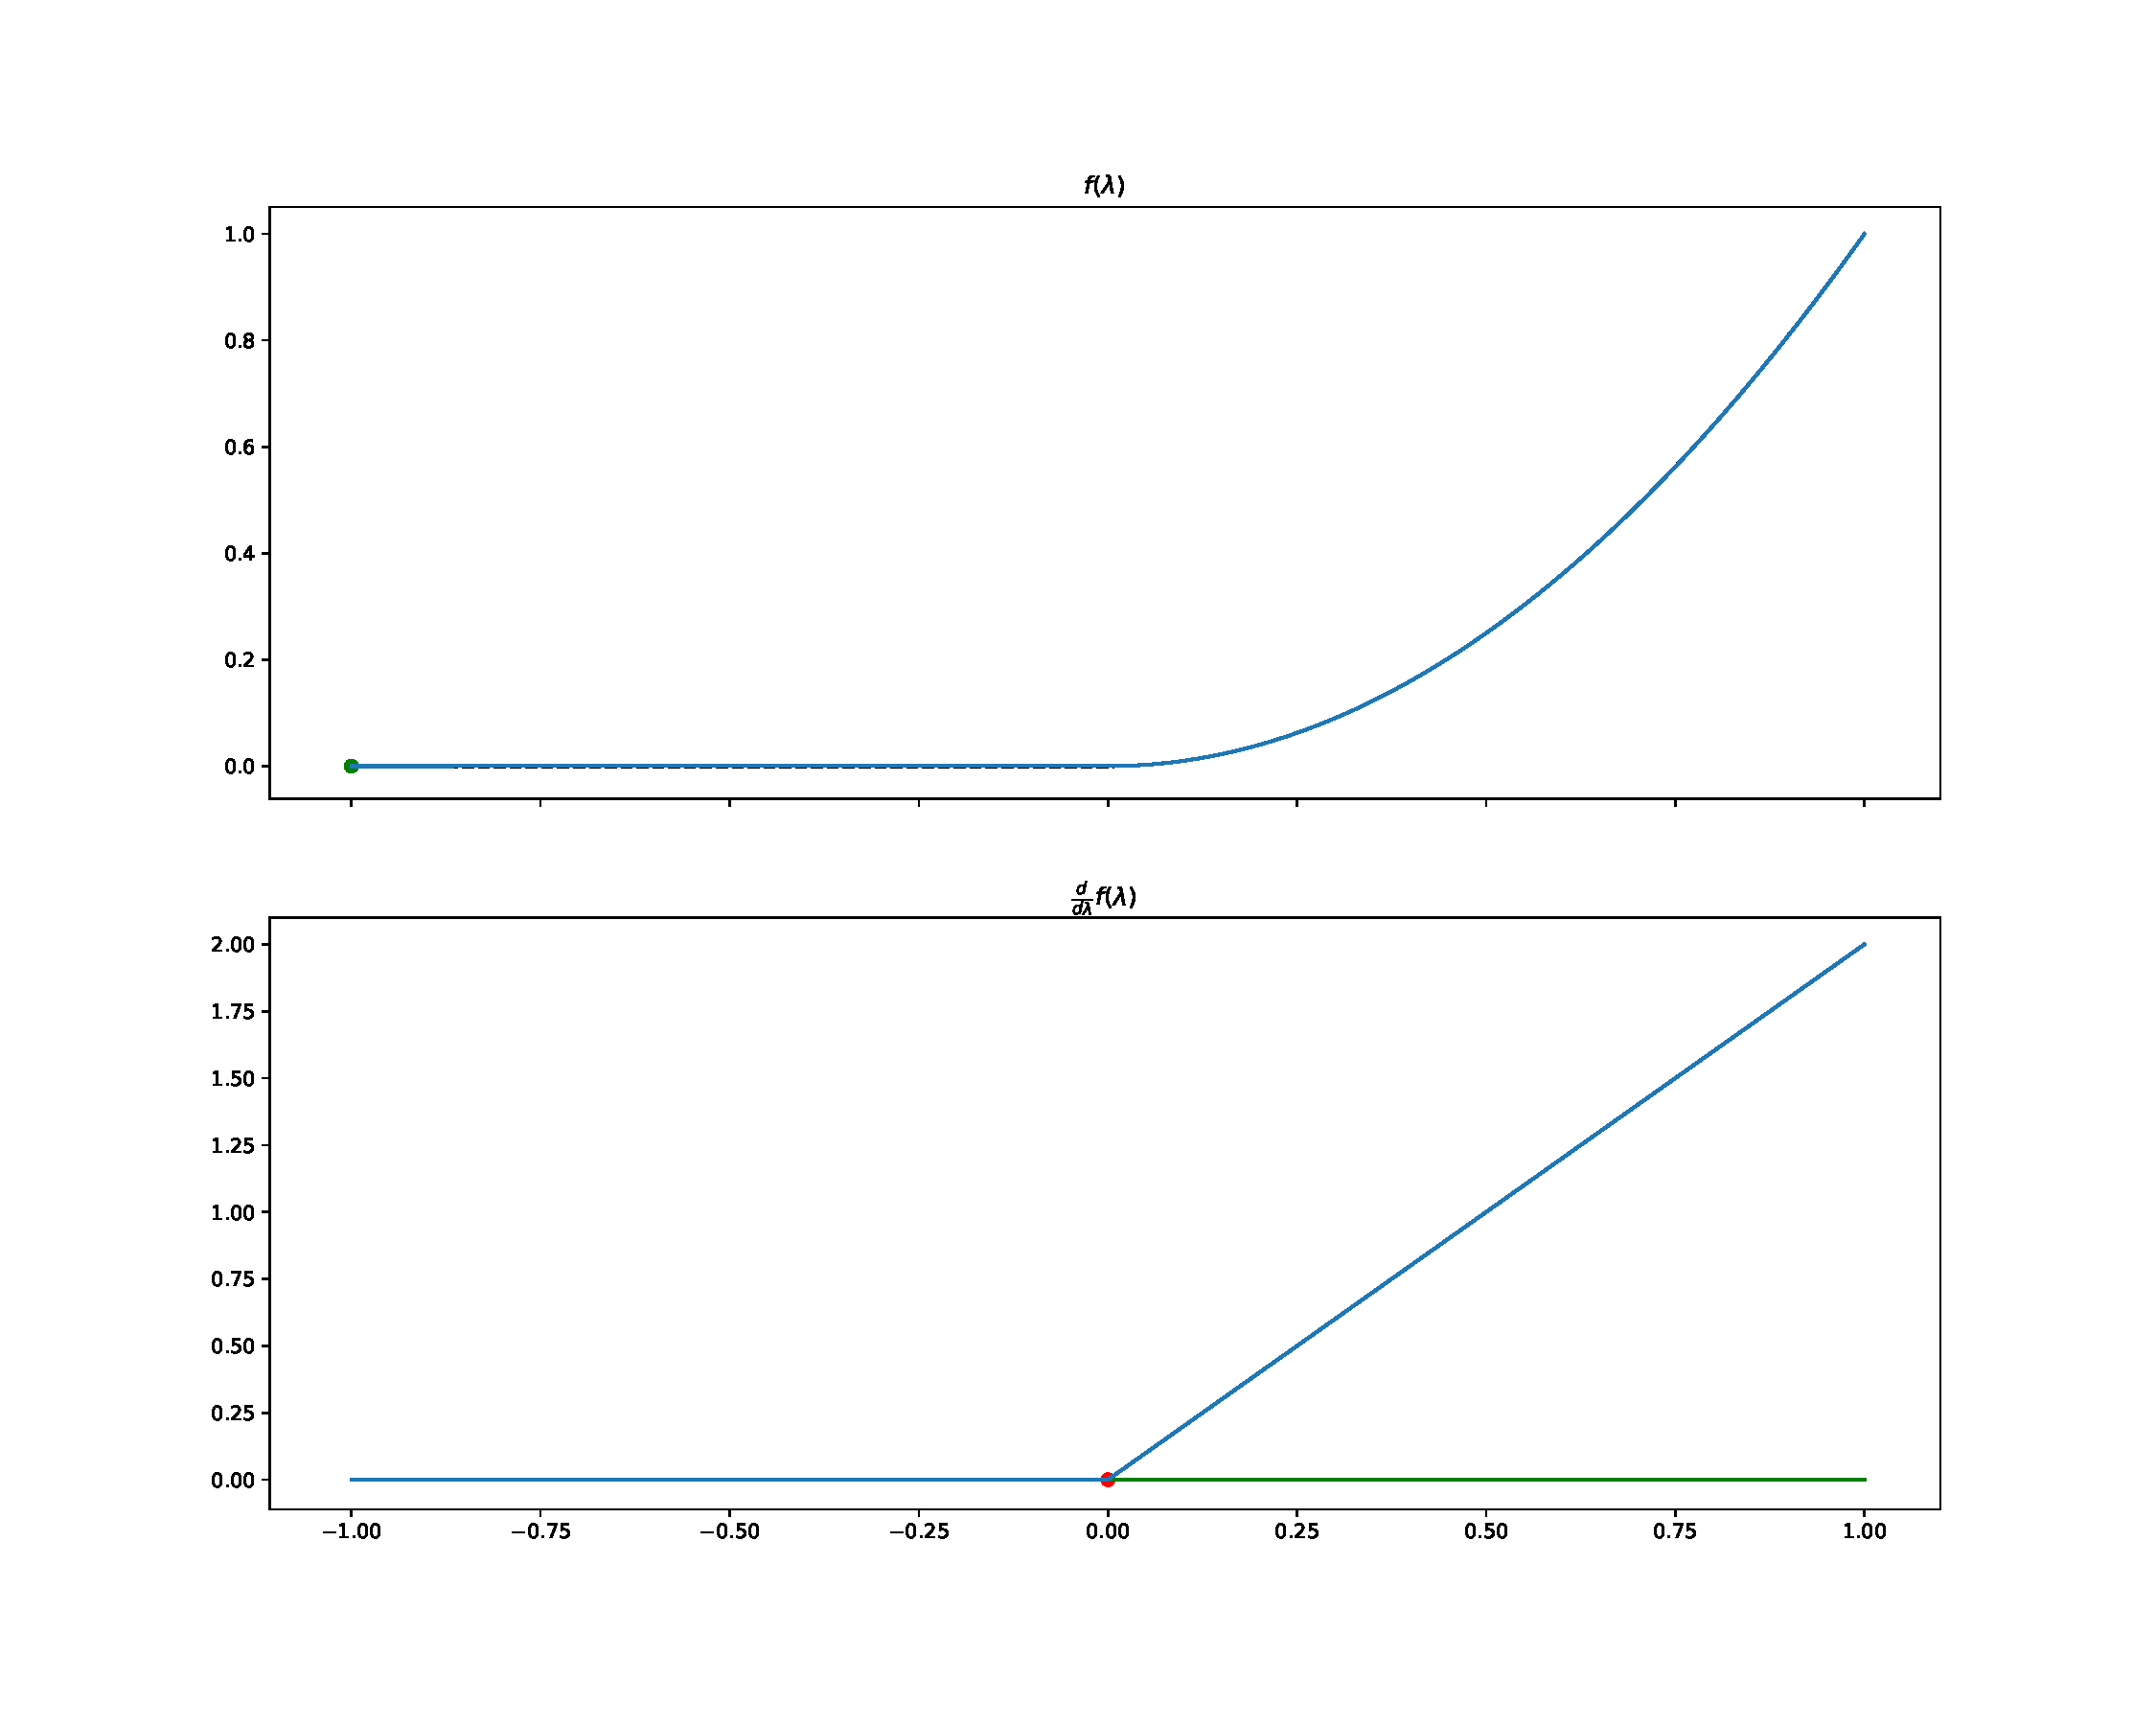
\includegraphics[width=\textwidth]{Chapter4/NeuroCom2021/ejemplo1_sqhinge.pdf}
    \caption{Positive part function (top) and its corresponding subgradient (bottom). The green line represents the $0$ constant function. The yellow dot indicates the point minimizing the function.}
    \label{fig:sqhinge_loss}
\end{figure}
Using the formulation of~\eqref{eq:subproblem_lambda}, the training error corresponding to the hinge loss is
\begin{equation}
    \label{eq:opt_hinge_l2}
    \argmin_{\lambda \in [0, 1]} \mathcal{J}(\lambda) = \sum_{i=1}^{\npertask} \pospart{\lambda c_i + d_i}^2.
\end{equation}
In each term of the sum the subdifferential is 
\begin{align*}
    \partial \left[\lambda c_i + d_i \right]_+^2 = 
    \begin{cases}
        0 &, \lambda c_i + d_i  \leq 0 \\
        2 c_i (\lambda c_i + d_i) &, \lambda c_i + d_i  > 0 \\
    \end{cases} \; .
\end{align*}
The elbows are again related to the values $\frac{-d_i}{c_i}$, that can be clipped and sorted to obtain the elbows ${\lambda}_{(1)} < \ldots < {\lambda}_{(m)}$.
In~\citet[Proposition 2]{RuizAD21} we give a result to get the optimal $\lambda^*$ when using the squared hinge loss.
\begin{prop}[Optimal $\lambda^*$ with squared hinge loss]\label{prop:sqhinge_neurocom2020}
    In~\eqref{eq:opt_hinge_l2},
    $\lambda^*=0$ is optimal iff 
    \begin{equation}\nonumber
         - \frac{\sum_{j: \lambda_{j} < 0} \max(0, c_{j}) d_{j} + \sum_{j: \lambda_{j} > 0} \min(0, c_{j}) d_{j}}{\sum_{j: \lambda_{j} < 0} \max(0, c_{j})^2 + \sum_{j: \lambda_{j} > 0} \min(0, c_{j})^2} < 0.
       \end{equation}
    If this condition does not hold, 
    consider the extended sorted list of feasible elbows $\lambda_{(p-1)} = 0 \leq \lambda_{(p)} \leq \ldots, \lambda_{(q)} \leq \lambda_{(q+1)}=1$, with $1 \leq p, q \leq m$, and
    define for $k=p-1, \ldots,  q$ $\widehat{\lambda}_k$ as %
\begin{equation}\label{sol_hinge_2}
 \widehat{\lambda}_k = - \frac{\sum_{j: \lambda_{(j)} < \lambda_{(k)}} \max(0, c_{j}) d_{j} + \sum_{j: \lambda_{(j)} > \lambda_{(k)}} \min(0, c_{j}) d_{j}}{\sum_{j: \lambda_{(j)} < \lambda_{(k)}} \max(0, c_{j})^2 + \sum_{j: \lambda_{(j)} > \lambda_{(k)}} \min(0, c_{j})^2} .
\end{equation}
%
Then, if $\lambda_k \leq \widehat{\lambda}_k \leq  \lambda_{k+1}$ for some $\widehat{\lambda}_k$, then $\lambda^* = \widehat{\lambda}_k$ is optimal.
Finally, if none of the previous conditions holds, \eqref{eq:opt_hinge_l2} has a minimum at $\lambda^* = 1$.
\end{prop}
\begin{figure}[t!]
    \centering
    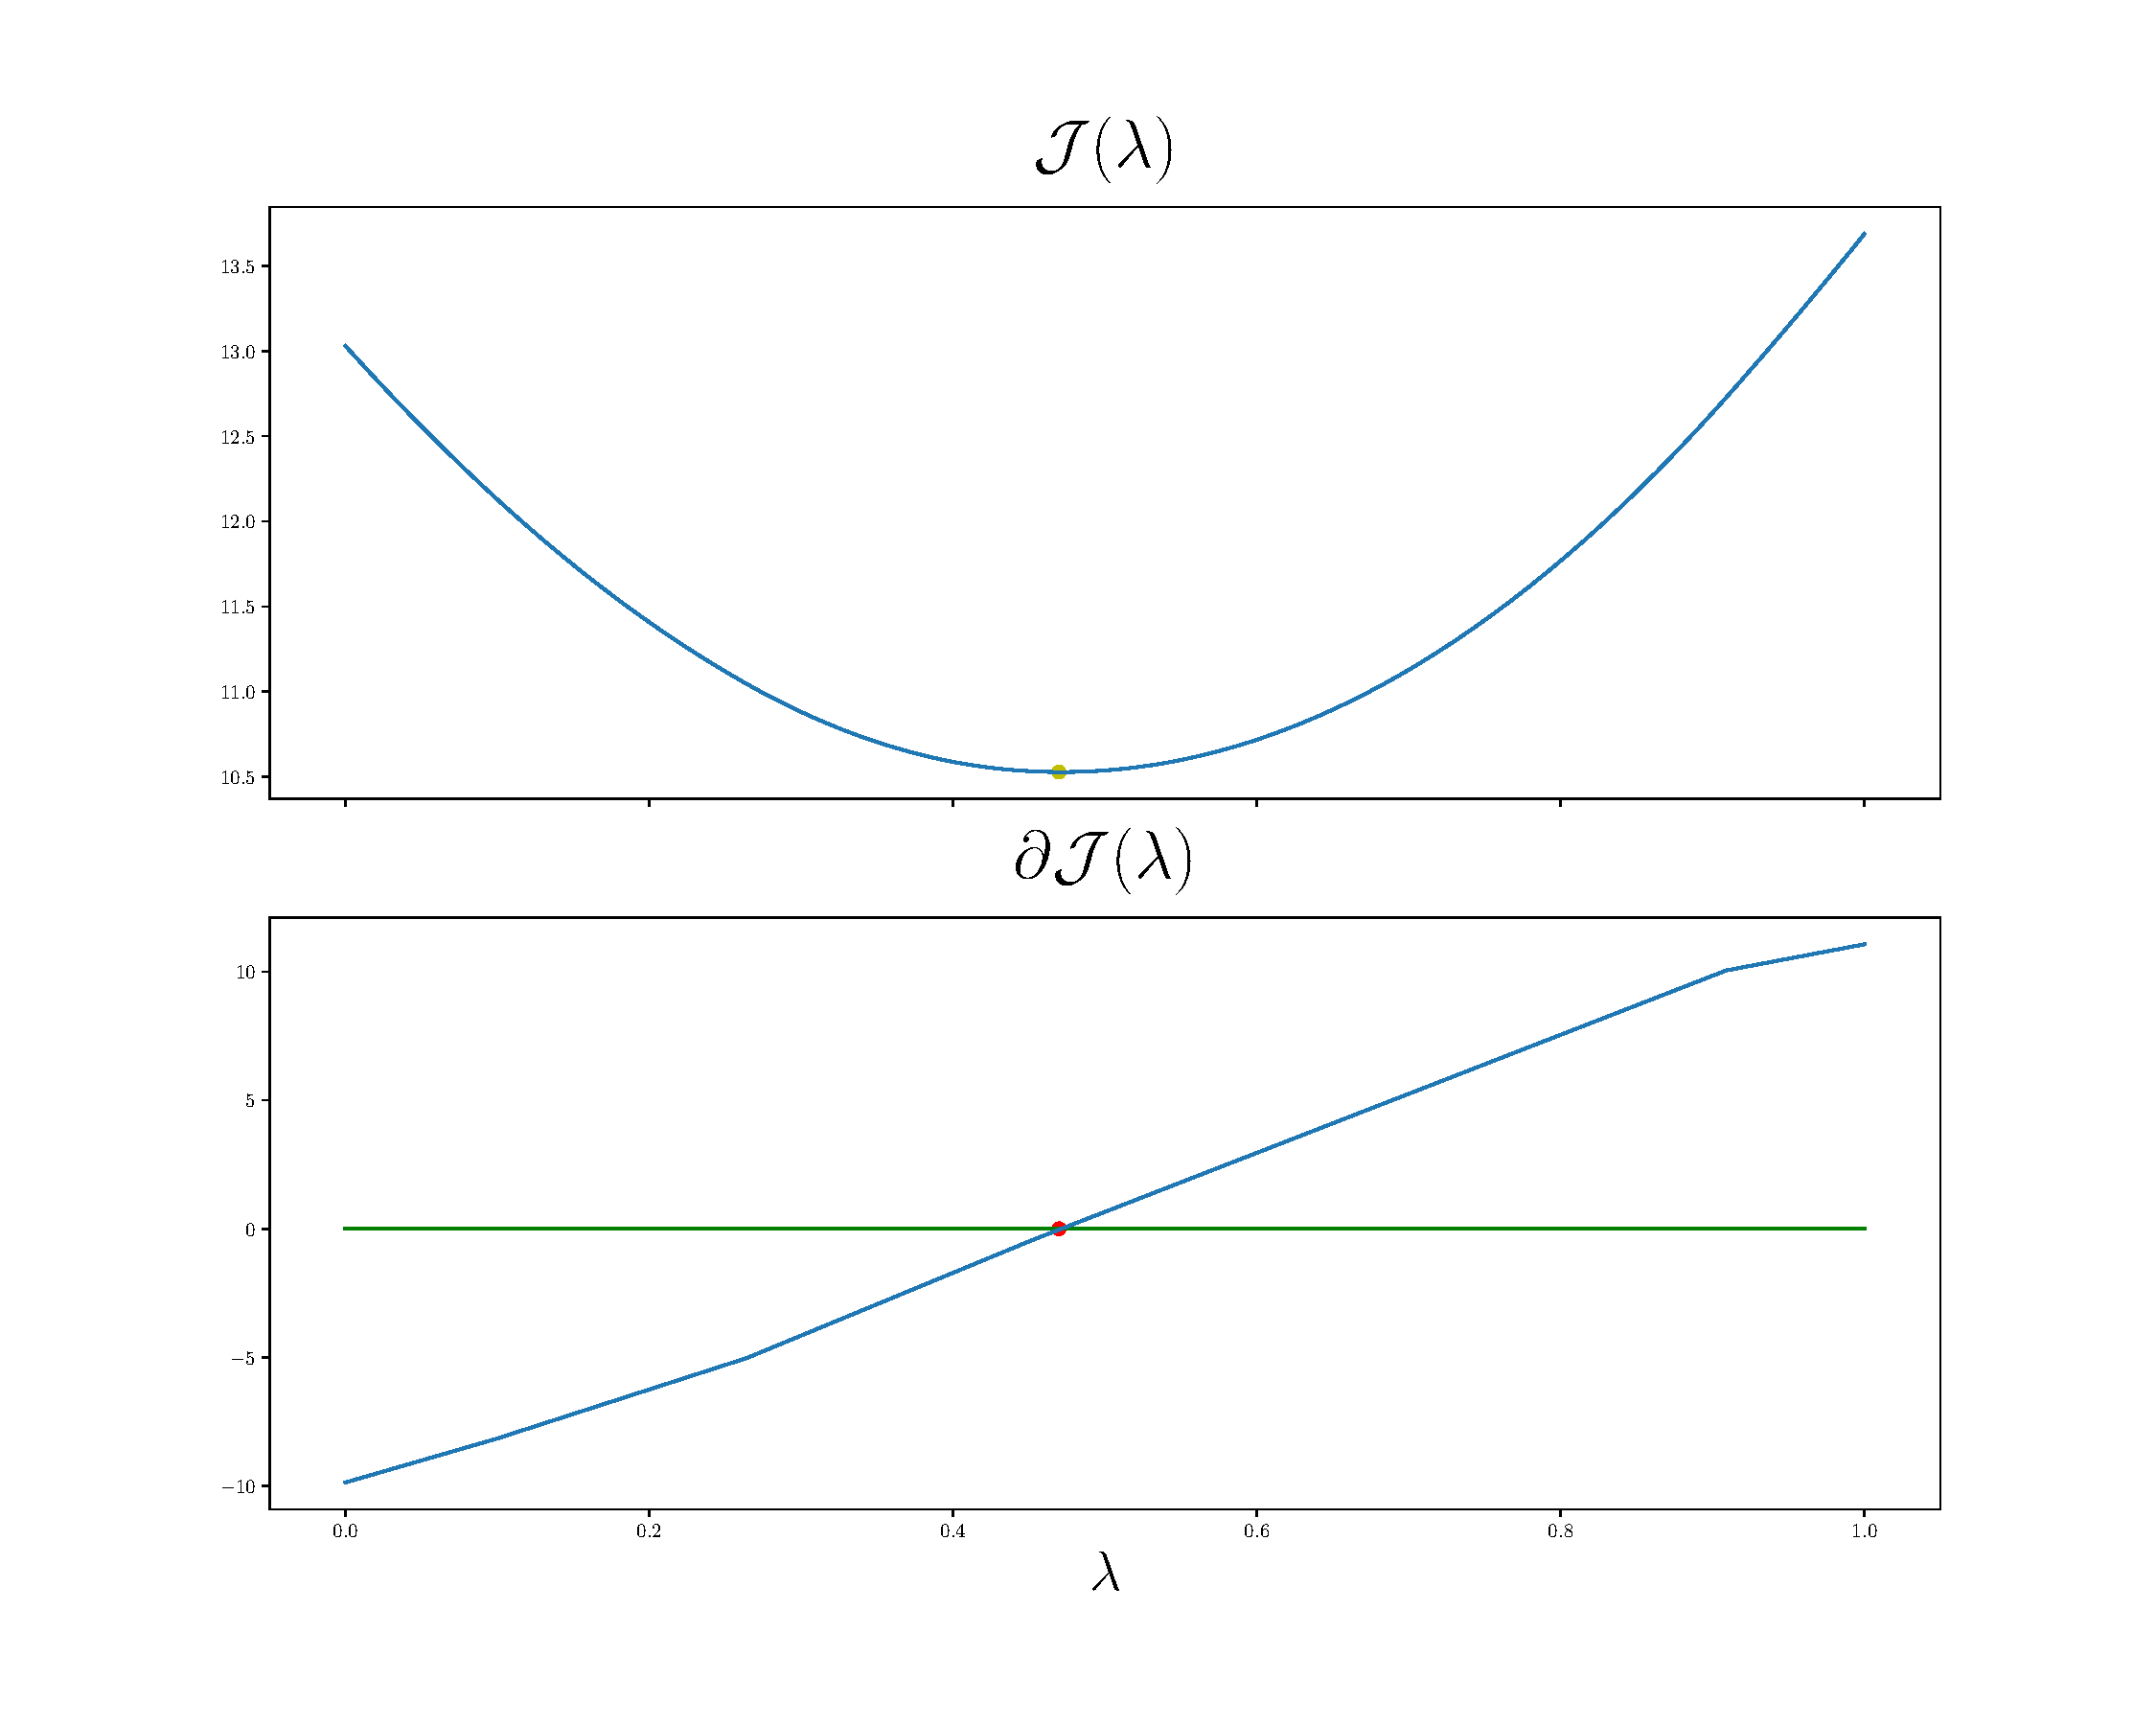
\includegraphics[width=\textwidth]{Chapter4/NeuroCom2021/ejemplo2_sqhinge.pdf}
    \caption{Error using squared hinge loss function (top) and its corresponding subgradient (bottom). The green line represents the $0$ constant function. The yellow dot is the point minimizing the error, and whose corresponding subgradient contains the value $0$.}
    \label{fig:sqhinge_error}
\end{figure}

As with the other losses, the error function and respective gradient for $10$ random pairs $(c_i, d_i)$ are represented in Figure~\ref{fig:sqhinge_error}.





\subsection{Experiments}\label{subsec:convexmtlsvm_exp}
In this subsection we show the experiments used to test the convex MTL formulation with kernel models, which have been presented in~\citep{RuizAD19} and~\citep{RuizAD21}. 
%
First, following the work in~\citep{RuizAD19}, experiments comparing convex and additive MTL formulations in the L1-SVM are described. 
%
Then, the experiments of~\citep{RuizAD21} are exposed, where all convex MTL models using L1, L2 and LS-SVMs as well as optimal convex combination of pre-trained models are compared using multiple real problems.

Before diving into the results, some technical details have to be explained. The convex MTL formulation, as presented in Equation~\eqref{eq:svmmtl_primal_convex}, uses task-specific hyperparameters $\lambda_r$, as well as common and task-specific kernels, with their corresponding hyperparameters; however, the selection of hyperparameters is always a challenge because of the curse of dimensionality. 
%
To select the hyperparameters $p_1, \ldots, p_L$ of a learning algorithm using CV the following problem is solved:
\begin{equation}
    \label{eq:hp-selection_general}
    p_1^*, \ldots, p_L^* = \argmin_{p_i \in \mathcal{S}_{p_i}, i=1, \ldots, L} \sum_{j=1}^{F} \rho(\mathcal{A}(p_1, \ldots, p_L; (X^j_\text{train}, y^j_\text{train})); (X^j_\text{val}, y^j_\text{val})) ,
\end{equation}
where $\rho$ is some measure, $\mathcal{A}$ is our choice of learning algorithm; $p_1, \ldots, p_L$ are the parameters on which $\mathcal{A}$ depends and $\mathcal{S}_{p_i}$ a feasible space for the parameter $p_i$; and $(X^j_\text{train}, y^j_\text{train}), (X^j_\text{val}, y^j_\text{val})$ are the training and validation sets, respectively. We are using $F$ folds, that is, for $j=1, \ldots, F$ we select different training and validation sets and we train our algorithm $\mathcal{A}$ on the training set $(X^j_\text{train}, y^j_\text{train})$, then we use $\rho$ to measure the wellness of our model on $(X^j_\text{val}, y^j_\text{val})$. 
%
Observe that our search space is the product space $\mathcal{S}_{p_1} \times \ldots \times \mathcal{S}_{p_L}$, so the difficulty of selecting an optimal combination of hyperparameters scales exponentially with the number of such parameters.

%
In a standard Gaussian kernel SVM, the definition of the problem depends on two hyperparameters: $C$ and $\gamma$.
In the L1 and L2-SVM for regression problems we also add a third parameter: $\epsilon$. 
That is, to select the hyperparameters of a standard SVM for a single task we have to solve the problem
\begin{equation}
    \nonumber
    C^*, \gamma^* (, \epsilon^*) = \argmin_{\substack{C \in \mathcal{S}_C ; \\ \substack{\gamma \in \mathcal{S}_\gamma} ; \\ \left(\substack{\epsilon \in \mathcal{S}_\epsilon} \right); }}
     \sum_{j=1}^{F} \rho(\mathcal{A}(C, \gamma (, \epsilon); (X^j_\text{train}, y^j_\text{train})); (X^j_\text{val}, y^j_\text{val})) ,
\end{equation}
which is typically feasible by using a grid search method in the space $\mathcal{S}_{C} \times \mathcal{S}_{\gamma} (\times \mathcal{S}_{\epsilon}) .$
%

However, using the convex MTL formulation, 
%as shown in the MTL kernel expression~\eqref{eq:conv_mtl_kernel_fun}, there are a common width $\gamma$ and task-specific widths $\gamma_1, \ldots, \gamma_\ntasks$.
we have the following hyperparameters: the regularization parameter $C$; the common kernel width $\gamma$, and task-specific ones $\gamma_1, \ldots, \gamma_\ntasks$; and the convex combination parameters $\lambda_1, \ldots, \lambda_\ntasks$; and possibly the $\epsilon$ parameter. That is, there are at least $2\ntasks + 2$ hyperparameters that have to be selected. Even with $\ntasks=2$, a search space of dimension $6$ is computationally unfeasible to cover.
% \begin{equation}
%     \nonumber
%     C^*, \gamma^*, \gamma_1^*, \ldots, \gamma_\ntasks^*, \lambda_1^*, \ldots, \lambda_\ntasks^*   (, \epsilon^*) = \argmin_{\substack{C \in \mathcal{S}_C ; \\ \substack{\gamma \in \mathcal{S}_\gamma} ; \\ \left(\substack{\epsilon \in \mathcal{S}_\epsilon} \right); }}
%      \sum_{j=1}^{F} \rho(\mathcal{A}(C, \gamma (, \epsilon); (X^j_\text{train}, y^j_\text{train})); (X^j_\text{val}, y^j_\text{val})) ,
% \end{equation}

To solve this difficulty and select the optimal parameters for the convex MTL formulation we follow the following strategy.
%
For the kernel widths, we proceed as follows: we first hyperparametrize the corresponding CTL and ITL kernel models, which have a common and task-specific kernel widths, respectively. 
Observe that in the CTL approach where a single virtual task is solved and in the ITL approach, where we solve the tasks independently, we have $2$ or $3$ parameters. We solve problems, which are represented in Equation~\eqref{eq:hp-selection_general}, using standard methods, and we obtain optimal common $C^*, \gamma^*$ and task-specific ones $C_r^*, \gamma^*_r$ for $r=1, \ldots, \ntasks$.
Then, we reutilize the optimal widths for these models, and fix them in the MTL one.
%
Moreover, for the convex combination parameters we use a single $\lambda$ for all tasks, that is, $\lambda_1 = \ldots = \lambda_\ntasks = \lambda$.
%
With these considerations, the problem to select the remaining hyperparameters is 
\begin{equation}
    \nonumber
    C^*, \lambda^* (, \epsilon^*) = \argmin_{\substack{C \in \mathcal{S}_C ; \\ \substack{\lambda \in \mathcal{S}_\lambda} ; \\ \left(\substack{\epsilon \in \mathcal{S}_\epsilon} \right); }}
     \sum_{j=1}^{F} \rho(\mathcal{A}(C, \lambda, \gamma^*, \gamma_1^*, \ldots, \gamma_\ntasks^* (, \epsilon); (X^j_\text{train}, y^j_\text{train})); (X^j_\text{val}, y^j_\text{val})) ,
\end{equation}
where we have a maximum of $3$ hyperparameters.

%
These are the two adjustments that we make to carry out the experiments shown in this subsection.
The first adjustment concerning kernel widths does not change the model definition, but it assumes that kernel widths that are good for CTL or ITL models are good for the MTL one. This assumption is a sensible one, since kernel widths are not that descriptive of the model but of the data used. The combined data from all tasks, which is used in CTL approach, is well ``characterized'' by a width $\sigma^*$ so we expect that this width is also useful for the common part of the MTL model. The same reasoning applies to task-specific data and ITL approach.
%
The second adjustment does change the models definition, using a single $\lambda$ that determines the specifity of all models. However, we expect that the possible difference in specifity among tasks can be corrected in the training process by selecting larger task-specific weights $v_r$ if necessary.

\paragraph*{Comparison of Convex and Additive Formulations.\\}
% Figure Synthetic Problem HAIS2019
\begin{figure}
    \centering
    \begin{subfigure}[b]{0.45\textwidth}
        \centering
        \includegraphics[width=\textwidth]{Chapter4/HAIS2019/synthetic_example-crop.pdf}
    \end{subfigure}
    \hfill
    \begin{subfigure}[b]{0.45\textwidth}
        \centering
        \includegraphics[width=\textwidth]{Chapter4/HAIS2019/synthetic_comparison-crop.pdf}
    \end{subfigure}
    \caption{Left: Synthetic example dataset, where the data of each task (corresponding to a different function $f_i$) are represented with a different color.
        Right: Comparison of the weights obtained by the {convex} and {additive} approaches.}
    \label{fig:lines_slopes}
\end{figure}

% Figure Convex vs Additive HAIS2019
\begin{figure}
    \centering
    \begin{subfigure}[b]{0.45\textwidth}
        \centering
        \includegraphics[width=\textwidth]{Chapter4/HAIS2019/synthetic_specWeights_add-crop.pdf}
    \end{subfigure}
    \hfill
    \begin{subfigure}[b]{0.45\textwidth}
        \centering
        \includegraphics[width=\textwidth]{Chapter4/HAIS2019/synthetic_specWeights_conv-crop.pdf}
    \end{subfigure}
    \caption{{Convex} (right) and {additive} (left) MTLSVR slope estimates weights as a function of $\lambda$. We represent the common part of the models, $w$ for the {additive} and $\lambda u$ for the {convex}, as well as each task specific deviation $v_t$ and $(1 - \lambda) u_t$.}
    \label{fig:synthetic_specWeights}
\end{figure}

%The work shown in~\cite{RuizAD19} focuses on 

In~\citep{RuizAD19}, we illustrate the results of equivalence between the additive and convex formulations in an empirical way. To do this we generate a synthetic problem, shown in Figure~\ref{fig:lines_slopes}, left, as a four linear regression tasks problem. 
%
We use four different functions $f_0, f_1, f_2, f_3$ by considering a base function $f(x) = 2x - 1$ with slope $m=2$ and bias $n=1$, then we sample $z_m^r, z_n^r \sim \normal{0, 1}$ for each task $r=0, \ldots, 3$ and create the $r$-th slope and bias by adding these Gaussian samples, i.e., $m_r = m + z_m^r$ and $n_r = n + z_n^r$. Also, we sample the noise $\sigma_r$ for each task uniformly in $(0, 5)$. 
%
Then, the $r$-th task consists on estimating $m_r$ and $n_r$ from data. To do this, for each task we uniformly sample $30$ points $x_i^r \in [1, 50)$, and the target values are defined as $y_i^r = f_r(x_i^r) + \epsilon^i_r$ where $\epsilon^i_r \sim \normal{0, \sigma_r}$.
%
Combining all tasks, there are $120$ data points, $30$ for each task, that we split randomly in a stratified way: two thirds, i.e. $80$ points are used for training, and the rest are used for testing purposes; in this division, the task size proportions are kept constant, that is $1/4$ for each task, in both the train and test sets. 
%
With this synthetic problem, we train four convex MTL models corresponding to values of $\lambda \in \set{0.2, 0.4, 0.6, 0.8}$; and we also train the corresponding equivalent additive MTL models, in which we set $\mu = (1 - \lambda)/\lambda^2$ and $C_\text{add} = (1 - \lambda)^2 C_\text{conv}$, as shown in Proposition~\ref{prop:add_conv_equiv}.
%
Our goal is to compare the influence of $\mu$ with that of $\lambda$ in the final models that are obtained. To do that, we need $C$ to be small enough so the regularization and, therefore, $\mu$ are relevant; the value $C_{\text{conv}} = 10^{-2}$ is found to be useful. We also consider linear kernels, so we can obtain the primal coefficients, that is, the slopes, and compare those obtained using the additive and convex formulations. In Figure~\ref{fig:lines_slopes}, right, we show the estimated slopes for each of the $\lambda$ values considered with a different color. In the $x$ axis we represent the convex slopes and in the $y$ axis the additive ones. There are four dots of each color, corresponding to each of the tasks considered in our synthetic problem. We can observe that all dots lie in the diagonal line corresponding to the identity function, as we expected from the equivalence result from Proposition~\ref{prop:add_conv_equiv}.

%
To further compare the two formulations, to visualize how the change on the hyperparameters imposes a change on the final models. Using the already described synthetic problem of Figure~\ref{fig:lines_slopes}, left, we select values of $\lambda$ ranging from $0$ to $1$, and their corresponding values $\mu = (1-\lambda)^2 / \lambda^2$, and fit convex and additive MTL linear SVMs using these values. In Figure~\ref{fig:synthetic_specWeights} we show the coefficients obtained for the common and task-specific parts with the additive formulation (left) and convex one (right).
%
We can observe how both graphics show a similar behaviour, with the common model starting in $0$ when $\mu$ is large or $\lambda=0$, and, as $\mu$ decreases and $\lambda$ grow, the task-specific parts go to zero and the common model reaches the optimal value for CTL.
%
However, two facts are noticeable, the first one is the range of hyperparameters needed for each formulation; while the convex formulation always uses $[0, 1]$, with the additive formulation it seems that $(10^{-3}, 10^3)$ is useful in this problem, but we cannot extrapolate to other problems; the second one is the smoother transition of the convex formulation, where the changes are steadily made, while with the additive one the changes look more abrupt.



\paragraph*{Performance of Convex MTL and Optimal Convex Combination.\\}

To test the performance of the convex MTL formulation, in~\citep{RuizAD19} we also conduct experiments with real problems, which are extended in~\citep{RuizAD21}. 
% Models
\paragraph*{Models.}
Considering that {LX} can stand for {L1}, {LS} or {LS}, we use the following approaches:
\begin{itemize}
    \item {Common Task Learning LX-SVM (\fmod{CTL-LX})}: A single LX-SVM which is fitted using data from all the tasks and does not use of the task information.
    \item {Independent Task Learning LX-SVM (\fmod{ITL-LX})}: Multiple task-specific LX-SVMs, each of which is fitted with the data from its own task.
    \item {Direct Convex Combination of LX-SVMs (\fmod{cvxCMB-LX})}: A combination of the best \fmod{CTL-LX} and \fmod{ITL-LX} as described in Subsection~\ref{subsec:optimal_comb}.
    \item {Convex Multi-Task Learning LX-SVM (\fmod{cvxMTL-LX})}: The Convex MTL formulations shown in Subsection~\ref{subsec:cvx_l1-svm} for the L1-SVM and in Subsection~\ref{subsec:cvx_l2ls-svm} for the L2- and LS-SVM.
\end{itemize}

% Problems
\paragraph*{Problems.}
To compare these approaches we will use several regression and classification problems. We use a total of six regression problems:
\begin{itemize}
    \item \fdata{majorca}: The goal is to predict the photovoltaic energy production of a park installed in Mallorca. The tasks are defined as the energy prediction at each hour with sunlight (we remove the night hours).
    \item \fdata{tenerife}: The goal is to predict the photovoltaic energy production of a park installed in Tenerife. The tasks are defined as the energy prediction at each hour with sunlight (we remove the night hours).
    \item \fdata{boston}: This is the housing problem in Boston, where the goal is to predict house prices, and the tasks are defined as the predictions in different areas of the city. In Boston we have the houses that are next to the river and those that are not.
    \item \fdata{california}: This is the housing problem in California, where the goal is also to predict house prices. Here the tasks correspond to 4 different areas of the city, related to their distance to the sea.
    \item \fdata{abalone}: The goal is to predict the number of rings of a specie of marine molluscs. The tasks are male, female or infant.
    \item \fdata{crime}: The goal is to predict the number of crimes per $100.000$ habitants in the U.S., the tasks are the prediction of the crime rate in different states.
\end{itemize}
For the classification setting, we consider eight problems, six of which are generated by applying different task definitions to two different problems.
\begin{itemize}
    \item \fdata{landmine}: This is a binary classification problem in which the goal is to detect landmines. Detection of different types of landmines determines a different task each. 
    \item \fdata{binding}: This is a binary classification problem where the goal is to determine if a given molecule will bind peptides. Different molecules define different tasks.
    \item \fdata{adult}: The goal is to predict whether the salary of a particular person is greater than 50K based on sociocultural data. We can define different tasks dividing the population by either gender or race, so we have the problems:
    \begin{itemize}
        \item \fdata{ad\_\{G\}}: dividing by gender
        \item \fdata{ad\_\{R\}}: dividing by race
        \item \fdata{ad\_\{G, R\}}: dividing by both gender and race
    \end{itemize}
    \item \fdata{compas}: The goal is to predict whether the COMPAS algorithm will assign "low" or "high" scores of recidivism to a particular subject. We can also divide the sample by either race or gender, so we obtain:
    \begin{itemize}
        \item \fdata{comp\_\{G\}}: dividing by gender
        \item \fdata{comp\_\{R\}}: dividing by race
        \item \fdata{comp\_\{G, R\}}: dividing by both gender and race
    \end{itemize}
\end{itemize}
The characteristics of some of the problems considered are present in Table~\ref{tab:mtl_problems} but, considering the different task definitions for \fdata{compas} and \fdata{adult} we give a more complete table in Table~\ref{tab:problems_hais19}.

% Table Problems HAIS19
\begin{table*}[t!]
    \caption{Sample sizes, dimensions and number of tasks of the datasets used.}
    \label{tab:problems_hais19}
    \centering
    \scalebox{.65}{
    \begin{tabular}{l*{7}{S[table-format=5]}}
    \toprule
    \fhead{Dataset} & \fhead{Size} & \fhead{No. feat.} & \fhead{No. tasks} & \fhead{Avg. task size} & \fhead{Min. t. s.} & \fhead{Max. t. s.}\\
    \midrule
    \fdata{majorca} & 15330 & 765 & 14 & 1095 & 1095 & 1095 \\ 
    \fdata{tenerife} & 15330 & 765 & 14 & 1095 & 1095 & 1095 \\
    \fdata{california} & 19269 & 9 & 5 & 3853 & 5 & 8468\\
    \fdata{boston} & 506 & 12 & 2 & 253 & 35 & 471 \\
    \fdata{abalone} & 4177 & 8 & 3 & 1392 & 1307 & 1527 \\
    \fdata{crime} & 1195 & 127 & 9 & 132 & 60  & 278 \\
    \fdata{binding} & 32302 & 184 & 47 & 687 & 59 & 3089 \\ 
    \fdata{landmine} & 14820 & 10 & 28 & 511 & 445 & 690 \\
    \fdata{adult\_(G)} & 48842 & 106 & 2 & 24421 & 16192 & 32650 \\
    \fdata{adult\_(R)} & 48842 & 103 & 5 & 9768 & 406 & 41762 \\
    \fdata{adult\_(G, R)} & 48842 & 101 & 10 & 4884 & 155 & 28735 \\
    \fdata{compas\_(G)} & 3987 & 11 & 2 & 1993 & 840 & 3147 \\
    \fdata{compas\_(R)} & 3987 & 9 & 4 & 997 & 255 & 1918 \\
    \fdata{compas\_(G, R)} & 3987 & 7 & 8 & 498 & 50 & 1525 \\
    \bottomrule
   \end{tabular}}
\end{table*}

% Experimental Procedure

% Table Hyperparameters HAIS19
\begin{table}[t]
    \caption{Hyperparameters, grids used to select them (when appropriate) and hyperparameter selection method for each model.}
    \label{tab:hyperpars_grid}
    \centering
    \scalebox{.65}{
     \begin{tabular}{*{9}{c}}
     \toprule
     \fhead{} & \fhead{Grid} & \fhead{\fmod{CTL-L1,2}} & \fhead{\fmod{ITL-L1,2}} & \fhead{\fmod{cvxMTL-L1,2}}  & \fhead{\fmod{CTL-LS}} & \fhead{\fmod{ITL-L,S}} & \fhead{\fmod{cvxMTL-LS}}   \\
     \midrule
      $C$ &  \scalebox{.9}{$\set{4^k: -2 \leq k \leq 6}$} & CV & CV & CV & CV & CV & CV  \\ 
      $\epsilon$ & \scalebox{.9}{$\set{\frac{\sigma}{4^k}: 1 \leq k \leq 6}$} & CV & CV & CV & - & - & - \\
      $\gamma_c$ & \scalebox{.9}{$\set{\frac{4^k}{d}: -2 \leq k \leq 3}$} & CV & - & \fmod{CTL-L1,2} & CV & - & \fmod{CTL-LS} \\
      $\gamma_s^r$ & \scalebox{.9}{$\set{\frac{4^k}{d}: -2 \leq k \leq 3}$} & - & CV & \fmod{ITL-L1,2} & - & CV & \fmod{ITL-LS}\\
      $\lambda$ & \scalebox{.9}{$\set{0.1 k : 0 \leq k \leq 10}$} & - & - & CV & - & - & CV \\
      \bottomrule
     \end{tabular}
     }
  \end{table}

\paragraph*{Experimental Procedure.}
To obtain the experimental results, we have to select the optimal hyperparameters for each model in a training-validation set and measure its performance on a test set. To do this, we follow the adjustments and experimental procedure described at the beginning of this subsection: reusing the kernel widths from CTL and ITL approaches and limiting the convex MTL formulation to a single parameter $\lambda$.
%
In all models considered we use Gaussian kernels, so all features have been scaled to the $[0, 1]$ interval.
As previously explained, the hyperparameters for the CTL and ITL approaches in the classification setting are $\set{C, \gamma}$ for all variants L1, L2 and LS-SVM.
In the regression setting we have $\set{C, \gamma, \epsilon}$ for the L1 and L2 variants, and $\set{C, \gamma}$ for the LS-SVM.
%
After selecting the optimal kernel widths in the CTL approach $\sigma^*$, and the task-specific widths $\sigma_r^*$ in the ITL approach, we use these values to fix them in the convex MTL formulation.
Then, the hyperparameters that we are considering for CV search in the convex MTL approaches in the classification settings are $\set{C, \lambda}$ for all variants, while in the regression problems they are $\set{C, \lambda, \epsilon}$ for the L1 and L2 variants and $\set{C, \lambda}$ for the LS-SVM.
%
The optimal combination approaches do not have proper hyperparameters, since $\lambda$ can be considered a training parameter.
%
In all problems, the hyperparameters considered are selected with a grid search using a task-stratified $3$-fold CV. That is, given a training-validation set, we divide it in three different folds where the task proportions are kept constant, and we use two of these folds for training the model and evaluate its performance in the remaining one.
%
In the regression problems, we will measure the validation performance using the MAE, see Table~\ref{tab:error_models_reg_mae_mae}, and MSE, see Table~\ref{tab:error_models_reg_mse_mae}.  Observe that the objective function of L1-SVM based models is more aligned with minimizing the MAE, while those of L2 and LS-SVM based models are more related to minimizing the MSE.
In the classification problems, see Table~\ref{tab:error_models_class_f1}, we will consider the F1 score to deal with the class-imbalance ratio that we find, for example, in the \fdata{landmine} dataset where we have 200 negative examples for every 13 positive ones.
%
In Table~\ref{tab:hyperpars_grid} we show for each hyperparameter of the considered approaches if they are selected using a CV procedure or recycling them from other approach, as well as the grids used for the CV search.

We have explained how we select the hyperparameters given a training-validation set, but it is necessary also to describe how we get the final results that we show on tables.
In every problem, except for \fdata{majorca} and \fdata{tenerife}, we will consider three external folds, each with the internal three folds for cross-validation. That is, the whole dataset of each problem is first divided in three task-stratified external folds: $F_1, F_
2, F_3$; then, two folds will form the training-validation set and the third one will be used as the test set. All folds have the same task proportions. There are three different combinations to do this division: $\set{F_1, F_2; F_3}, \set{F_1, F_3; F_2}$ and $\set{F_2, F_3; F_1}$, where the first two folds form the train-validation set and the other one is the test set.
%
In each train-validation set we follow the procedure described above to select the optimal hyperparameters, and the performance model with the optimal hyperparameters will be tested in the remaining fold, i.e., the test set.
%

The problems of \fdata{majorca} and \fdata{tenerife} have a temporal dependency, so it is not possible to use training data from a time that is ahead of that of the test or validation data. Therefore, we use data from years 2013, 2014 and 2015, each corresponding to train, validation and test sets, respectively.
%
We consider different metrics to measure the test performance. Therefore, in every problem, except \fdata{majorca} and \fdata{tenerife}, for each metric we obtain three different scores, each corresponding to a different test set, so we will show the mean and standard deviation of such scores. In \fdata{majorca} and \fdata{tenerife} we obtain a single test score corresponding to data from the year 2015.
% 
For the regression problems, in Tables~\ref{tab:error_models_reg_mae_mae} and~\ref{tab:error_models_reg_mse_mae}, we show both the MAE and R2 score, closely related to MSE, obtained in the test set, and for classification, in Table~\ref{tab:error_models_class_f1}, we show the F1 and the accuracy scores.
%




% Results


  \begin{table*}[t]
    \captionsetup{font=scriptsize}
    \caption{Test MAE (top) and R2 score (bottom) and Wilcoxon-based ranking for the models selected using the MAE for hyperparametrization. The best models are shown in bold.}
    \label{tab:error_models_reg_mae_mae}
    \centering
    \scalebox{.65}{
    \begin{tabular}{l*{2}{c@{ }l}*{4}{r@{$\pm$}l@{ }l } }
    \toprule
    & \fheadmulti{2}{\fdata{maj.}} & \fheadmulti{2}{\fdata{ten.}} & \fheadmulti{3}{\fdata{boston}} & \fheadmulti{3}{\fdata{california}} &  \fheadmulti{3}{\fdata{abalone}} & \fheadmulti{3}{\fdata{crime}}\\
    \midrule
    & \fheadmulti{16}{MAE} \\
    \midrule
    \fmod{ITL-L1}            &  {5.087} &   (6) &  {5.743} &   (3) &  {2.341} & {0.229} &   \fmaxn{(1)} &  {36883.582} & {418.435} &   (2) &  {1.481} & {0.051} &   (3) &  {0.078} & {0.001} &   (2) \\
    \fmod{CTL-L1}            &  {5.175} &   (7) &  {5.891} &   (5) &  \fmaxn{2.192} & \fmaxn{0.244} &   \fmaxn{(1)} &  {41754.337} & {270.908} &   (6) &  {1.482} & {0.050} &   (3) &  {0.078} & {0.001} &   (2) \\
    \fmod{cvxCMB-L1} &  \fmaxn{5.047} &   (5) &  \fmaxn{5.340} &  \fmaxn{(1)} &  {2.239} & {0.255} &   \fmaxn{(1)} &  {36880.238} & {420.417} &   \fmaxn{(1)} &  {1.470} & {0.052} &   (2) &  {0.077} & {0.002} &   (2) \\
    \fmod{cvxMTL-L1}     &  {5.050} &   (5) &  {5.535} &   (2) &  {2.206} & {0.292} &   \fmaxn{(1)} &  \fmaxn{36711.383} & \fmaxn{343.333} &  \fmaxn{(1)} &  \fmaxn{1.454} & \fmaxn{0.048} &  \fmaxn{(1)} &  \fmaxn{0.074} & \fmaxn{0.002} &  \fmaxn{(1)} \\
    \midrule
    \fmod{ITL-L2}            &  {4.952} &   (3) &  \fmaxn{5.629} &   (3) &  {2.356} & {0.300} &   \fmaxn{(1)} &  {37374.618} & {433.511} &   (5) &  {1.498} & {0.054} &   (4) &  {0.079} & {0.002} &   (2) \\
    \fmod{CTL-L2}            &  {5.193} &   (7) &  {6.107} &   (8) &  \fmaxn{2.083} & \fmaxn{0.136} &   \fmaxn{(1)} &  {42335.612} & {163.773} &   (8) &  {1.503} & {0.047} &   (5) &  {0.080} & {0.002} &   (2) \\
    \fmod{cvxCMB-L2} &  {4.869} &   (3) &  {5.963} &   (6) &  {2.089} & {0.128} &   \fmaxn{(1)} &  {37374.618} & {433.511} &   (4) &  {1.494} & {0.050} &   (4) &  {0.077} & {0.003} &   (2) \\
    \fmod{cvxMTL-L2}     &  \fmaxn{4.854} &   (2) &  {5.784} &   (4) &  {2.089} & {0.134} &   \fmaxn{(1)} &  \fmaxn{37202.603} & \fmaxn{419.166} &   (3) &  \fmaxn{1.482} & \fmaxn{0.049} &   (3) &  \fmaxn{0.077} & \fmaxn{0.002} &   (2) \\
    \midrule
    \fmod{ITL-LS}            &  {4.937} &   (3) &  {5.649} &   (3) &  {2.204} & {0.116} &   \fmaxn{(1)} &  {37348.347} & {441.240} &   (4) &  {1.496} & {0.051} &   (4) &  {0.079} & {0.002} &   (2) \\
    \fmod{CTL-LS}            &  {5.193} &   (7) &  {6.005} &   (7) &  \fmaxn{2.072} & \fmaxn{0.143} &  \fmaxn{(1)} &  {42259.492} & {146.825} &   (7) &  {1.502} & {0.052} &   (5) &  {0.079} & {0.002} &   (2) \\
    \fmod{cvxCMB-LS} &  {4.977} &   (4) &  \fmaxn{5.593} &   (3) &  {2.081} & {0.146} &   \fmaxn{(1)} &  {37339.179} & {430.288} &   (4) &  {1.486} & {0.049} &   (4) &  {0.079} & {0.002} &   (2) \\
    \fmod{cvxMTL-LS}     &  \fmaxn{4.824} &  \fmaxn{(1)} &  {5.754} &   (4) &  {2.077} & {0.152} &   \fmaxn{(1)} &  \fmaxn{37231.043} & \fmaxn{420.992} &   (4) &  \fmaxn{1.478} & \fmaxn{0.050} &   (3) &  \fmaxn{0.076} & \fmaxn{0.002} &   (2) \\
    \midrule
    & \fheadmulti{16}{R2} \\
    \midrule
    \fmod{ITL-L1}            &  {0.845} &   (6) &  {0.901} &   (7) &  {0.821} & {0.041} &   (2) &  {0.699} & {0.009} &   (7) &  {0.543} & {0.022} &   (8) &  {0.732} & {0.021} &   (3) \\
    \fmod{CTL-L1}            &  {0.837} &   (9) &  {0.901} &   (6) &  {0.854} & {0.036} &   \fmaxn{(1)} &  {0.639} & {0.006} &  (10) &  {0.559} & {0.014} &   (6) &  {0.740} & {0.027} &   (3) \\
    \fmod{cvxCMB-L1} &  {0.844} &   (6) &  {0.905} &   (4) &  {0.845} & {0.053} &   \fmaxn{(1)} &  {0.699} & {0.009} &   (6) &  {0.555} & {0.018} &   (7) &  {0.741} & {0.029} &   (3) \\
    \fmod{cvxMTL-L1}     &  \fmaxn{0.846} &   (4) &  \fmaxn{0.908} &   (2) &  \fmaxn{0.858} & \fmaxn{0.057} &   \fmaxn{(1)} &  \fmaxn{0.703} & \fmaxn{0.007} &   (6) &  \fmaxn{0.568} & \fmaxn{0.012} &   (5) &  \fmaxn{0.760} & \fmaxn{0.024} &   (2) \\
    \midrule
    \fmod{ITL-L2}            &  {0.846} &   (5) &  {0.906} &   (3) &  {0.836} & {0.045} &   (2) &  {0.707} & {0.009} &   (5) &  {0.565} & {0.025} &   (6) &  {0.743} & {0.017} &   (3) \\
    \fmod{CTL-L2}            &  {0.840} &   (8) &  {0.901} &   (8) &  \fmaxn{0.889} & \fmaxn{0.017} &   \fmaxn{(1)} &  {0.645} & {0.005} &   (9) &  {0.574} & {0.013} &   (4) &  {0.744} & {0.028} &   (3) \\
    \fmod{cvxCMB-L2} &  {0.850} &   (3) &  {0.900} &   (9) &  {0.885} & {0.013} &   \fmaxn{(1)} &  {0.707} & {0.009} &   (4) &  {0.571} & {0.018} &   (4) &  {0.755} & {0.024} &   (3) \\
    \fmod{cvxMTL-L2}     &  \fmaxn{0.863} &   (2) &  \fmaxn{0.908} &   \fmaxn{(1)} &  {0.888} & {0.015} &   \fmaxn{(1)} &  \fmaxn{0.709} & \fmaxn{0.008} &  \fmaxn{(1)} &  \fmaxn{0.580} & \fmaxn{0.014} &   (3) &  \fmaxn{0.762} & \fmaxn{0.028} &   \fmaxn{(1)} \\
    \midrule
    \fmod{ITL-LS}            &  {0.849} &   (3) &  {0.907} &   (3) &  {0.856} & {0.008} &   \fmaxn{(1)} &  {0.707} & {0.009} &   (3) &  {0.573} & {0.015} &   (4) &  {0.743} & {0.022} &   (3) \\
    \fmod{CTL-LS}            &  {0.838} &   (9) &  {0.904} &   (5) &  \fmaxn{0.894} & \fmaxn{0.015} &  \fmaxn{(1)} &  {0.646} & {0.005} &   (8) &  {0.576} & {0.016} &   (4) &  {0.746} & {0.032} &   (3) \\
    \fmod{cvxCMB-LS} &  {0.843} &   (7) &  {0.907} &   (2) &  {0.886} & {0.024} &   \fmaxn{(1)} &  {0.707} & {0.009} &   (2) &  {0.581} & {0.012} &   (2) &  {0.746} & {0.021} &   (3) \\
    \fmod{cvxMTL-LS}     &  \fmaxn{0.863} &  \fmaxn{(1)} &  \fmaxn{0.910} &  \fmaxn{(1)} &  {0.890} & {0.016} &   \fmaxn{(1)} &  \fmaxn{0.709} & \fmaxn{0.008} &   (2) &  \fmaxn{0.581} & \fmaxn{0.015} &  \fmaxn{(1)} &  \fmaxn{0.763} & \fmaxn{0.028} &  \fmaxn{(1)} \\
    \bottomrule
    \end{tabular}}
  \end{table*}





  \begin{table*}[t]
    \captionsetup{font=scriptsize}
    \caption{Test MAE (top) and R2 score (bottom) and Wilcoxon-based ranking for the models selected using the MSE for hyperparametrization. The best models are shown in bold.}
      \label{tab:error_models_reg_mse_mae}
      \centering
      \scalebox{.65
      }{
          \begin{tabular}{l*{2}{c@{ }l}*{4}{r@{$\pm$}l@{ }l } }
              \toprule
              & \fheadmulti{2}{\fdata{maj.}} & \fheadmulti{2}{\fdata{ten.}} & \fheadmulti{3}{\fdata{boston}} & \fheadmulti{3}{\fdata{california}} &  \fheadmulti{3}{\fdata{abalone}} & \fheadmulti{3}{\fdata{crime}}\\
      \midrule
      & \fheadmulti{16}{MAE} \\
      \midrule
      \fmod{ITL-L1}            &  {5.087} &   (7) &  {5.743} &   (3) &  {2.437} & {0.281} &   (3) &  {36941.516} & {450.767} &   (1) &  {1.480} & {0.058} &   (3) &  {0.079} & {0.002} &   (3) \\
      \fmod{CTL-L1}            &  {5.175} &   (8) &  {5.891} &   (7) &  {2.315} & {0.192} &   (2) &  {41857.602} & {235.021} &   (6) &  {1.479} & {0.047} &   (3) &  {0.078} & {0.000} &   (2) \\
      \fmod{cvxCMB-L1} &  \fmaxn{4.920} &   (4) &  {5.743} &   (4) &  {2.315} & {0.192} &   (3) &  \fmaxn{36941.476} & \fmaxn{450.711} &  \fmaxn{(1)} &  {1.471} & {0.057} &   (2) &  {0.079} & {0.002} &   (2) \\
      \fmod{cvxMTL-L1}     &  {5.050} &   (6) &  \fmaxn{5.535} &  \fmaxn{(1)} &  \fmaxn{2.244} & \fmaxn{0.150} &   (1) &  {36999.003} & {360.445} &   (2) &  \fmaxn{1.455} & \fmaxn{0.046} &  \fmaxn{(1)} &  \fmaxn{0.074} & \fmaxn{0.001} &  \fmaxn{(1)} \\
      \midrule
      \fmod{ITL-L2}            &  {4.924} &   (5) &  {5.752} &   (5) &  {2.437} & {0.324} &   (3) &  {37407.929} & {461.878} &   (5) &  {1.497} & {0.050} &   (5) &  {0.079} & {0.002} &   (2) \\
      \fmod{CTL-L2}            &  {5.193} &   (8) &  {6.107} &   (9) &  {2.096} & {0.112} &   (1) &  {42335.612} & {163.773} &   (7) &  {1.504} & {0.048} &   (6) &  {0.079} & {0.002} &   (2) \\
      \fmod{cvxCMB-L2} &  \fmaxn{4.813} &  \fmaxn{(1)} &  \fmaxn{5.623} &   (3) &  {2.116} & {0.131} &   (1) &  {37398.940} & {449.498} &   (5) &  {1.495} & {0.051} &   (5) &  {0.078} & {0.003} &   (2) \\
      \fmod{cvxMTL-L2}     &  {4.854} &   (4) &  {5.784} &   (6) &  \fmaxn{2.082} & \fmaxn{0.130} &   (1) &  \fmaxn{37356.599} & \fmaxn{390.629} &   (4) &  \fmaxn{1.481} & \fmaxn{0.041} &   (4) &  \fmaxn{0.076} & \fmaxn{0.000} &   (2) \\
      \midrule
      \fmod{ITL-LS}            &  {4.937} &   (5) &  {5.649} &   (3) &  {2.326} & {0.231} &   (3) &  {37385.244} & {403.331} &   (4) &  {1.495} & {0.045} &   (5) &  {0.079} & {0.002} &   (2) \\
      \fmod{CTL-LS}            &  {5.193} &   (8) &  {6.005} &   (8) &  \fmaxn{2.072} & \fmaxn{0.143} &  \fmaxn{(1)} &  {42339.063} & {156.624} &   (7) &  {1.504} & {0.043} &   (6) &  {0.078} & {0.002} &   (2) \\
      \fmod{cvxCMB-LS} &  \fmaxn{4.820} &   (2) &  {5.578} &   (2) &  {2.136} & {0.106} &   (1) &  {37377.005} & {391.694} &   (4) &  {1.491} & {0.048} &   (5) &  {0.078} & {0.002} &   (2) \\
      \fmod{cvxMTL-LS}     &  {4.824} &   (3) &  \fmaxn{5.754} &   (6) &  {2.090} & {0.090} &   (1) &  \fmaxn{37232.918} & \fmaxn{397.866} &   (3) &  \fmaxn{1.478} & \fmaxn{0.042} &   (3) &  \fmaxn{0.076} & \fmaxn{0.000} &   (2) \\
      \midrule
      & \fheadmulti{16}{R2} \\
      \midrule
      \fmod{ITL-L1}            &  {0.845} &   (6) &  {0.901} &   (9) &  {0.800} & {0.050} &   (3) &  {0.703} & {0.009} &   (8) &  {0.534} & {0.053} &  (10) &  {0.732} & {0.017} &   (4) \\
      \fmod{CTL-L1}            &  {0.837} &   (7) &  {0.901} &   (8) &  {0.860} & {0.026} &   (2) &  {0.642} & {0.006} &  (10) &  {0.564} & {0.011} &   (8) &  {0.748} & {0.017} &   (3) \\
      \fmod{cvxCMB-L1} &  \fmaxn{0.852} &   (4) &  {0.901} &  (10) &  {0.860} & {0.026} &   (3) &  {0.703} & {0.009} &   (7) &  {0.550} & {0.036} &   (9) &  {0.733} & {0.018} &   (3) \\
      \fmod{cvxMTL-L1}     &  {0.846} &   (5) &  \fmaxn{0.908} &   (5) &  \fmaxn{0.871} & \fmaxn{0.019} &   (1) &  \fmaxn{0.705} & \fmaxn{0.008} &   (6) &  \fmaxn{0.573} & \fmaxn{0.011} &   (7) &  \fmaxn{0.764} & \fmaxn{0.019} &   (1) \\
      \midrule
      \fmod{ITL-L2}            &  {0.850} &   (4) &  {0.906} &   (6) &  {0.819} & {0.053} &   (3) &  {0.707} & {0.009} &   (4) &  {0.573} & {0.020} &   (6) &  {0.744} & {0.018} &   (3) \\
      \fmod{CTL-L2}            &  {0.840} &   (6) &  {0.901} &  (11) &  {0.886} & {0.014} &   (1) &  {0.645} & {0.005} &   (9) &  {0.574} & {0.013} &   (6) &  {0.747} & {0.025} &   (3) \\
      \fmod{cvxCMB-L2} &  {0.857} &   (3) &  \fmaxn{0.910} &  \fmaxn{(1)} &  {0.883} & {0.016} &   (1) &  {0.707} & {0.009} &   (2) &  {0.574} & {0.021} &   (5) &  {0.751} & {0.029} &   (3) \\
      \fmod{cvxMTL-L2}     &  \fmaxn{0.863} &   (2) &  {0.908} &   (4) &  \fmaxn{0.887} & \fmaxn{0.015} &   (1) &  \fmaxn{0.708} & \fmaxn{0.007} &   (2) &  \fmaxn{0.581} & \fmaxn{0.011} &   (2) &  \fmaxn{0.768} & \fmaxn{0.020} &  \fmaxn{(1)} \\
      \midrule
      \fmod{ITL-LS}            &  {0.849} &   (4) &  {0.907} &   (5) &  {0.841} & {0.028} &   (3) &  {0.707} & {0.009} &   (5) &  {0.577} & {0.012} &   (4) &  {0.743} & {0.021} &   (3) \\
      \fmod{CTL-LS}            &  {0.838} &   (7) &  {0.904} &   (7) &  \fmaxn{0.894} & \fmaxn{0.015} &  \fmaxn{(1)} &  {0.645} & {0.005} &   (9) &  {0.575} & {0.012} &   (4) &  {0.754} & {0.022} &   (3) \\
      \fmod{cvxCMB-LS} &  {0.856} &   (3) &  {0.909} &   (3) &  {0.877} & {0.009} &   (1) &  {0.707} & {0.009} &   (3) &  {0.580} & {0.013} &   (3) &  {0.750} & {0.024} &   (3) \\
      \fmod{cvxMTL-LS}     &  \fmaxn{0.863} &  \fmaxn{(1)} &  \fmaxn{0.910} &   (2) &  {0.890} & {0.014} &   (1) &  \fmaxn{0.710} & \fmaxn{0.008} &  \fmaxn{(1)} &  \fmaxn{0.582} & \fmaxn{0.011} &  \fmaxn{(1)} &  \fmaxn{0.763} & \fmaxn{0.019} &   (2) \\
      \bottomrule
      \end{tabular}}
    \end{table*}
  



\begin{table*}[t]
    \captionsetup{font=scriptsize}
    \caption{Test F1 (top) and accuracy (bottom) scores, global and block-wise Wilcoxon-based rankings for classification problems. The best models in each block are shown in bold.}
    \label{tab:error_models_class_f1}
    \centering
    \scalebox{.65}{
      \begin{tabular}{ l*{8}{c} c c c}
        \toprule
        & \fhead{\fdata{comp\_(G)}} & \fhead{\fdata{comp\_(R)}} & \fhead{\fdata{comp\_(G,R)}} & \fhead{\fdata{ad\_(G)}} & \fhead{\fdata{ad\_(R)}} & \fhead{\fdata{ad\_(G,R)}} & \fhead{\fdata{landmine}} & \fhead{\fdata{binding}} & \fhead{mean} & \fhead{rank} & \fhead{Wil.}\\
        \midrule
        & \fheadmulti{8}{F1}  \\
        \midrule
        \fmod{ITL-L1}    &          0.625 &           \fmaxn{0.639} &                  0.630 &         \fmaxn{0.659} &          0.653 &                 0.657 &    0.231 &   0.867 & 0.620 &     10 & 1 \\
        \fmod{CTL-L1}    &          0.623 &           0.638 &                  0.638 &         0.657 &          0.650 &                 0.653 &    0.255 &   0.901 & 0.627 &      7 & 1 \\
        \fmod{cvxCMB-L1} &          0.616 &           0.638 &                  0.638 &         0.658 &          0.650 &                 0.653 &    \fmaxn{0.270} &   0.901 & \fmaxn{0.628} &      6 & 1 \\
        \fmod{cvxMTL-L1}    &          \fmaxn{0.627} &           0.636 &                  \fmaxn{0.640} &         \fmaxn{0.659} &          \fmaxn{0.655} &                 \fmaxn{0.659} &    0.242 &   \fmaxn{0.907} & \fmaxn{0.628} &      5 & 1 \\
        \midrule
        \fmod{ITL-L2}    &          0.636 &           0.623 &                  0.607 &         \fmaxn{0.668} &          \fmaxn{0.666} &                 \fmaxn{0.668} &    0.256 &   0.867 & 0.624 &      8 & 3 \\
        \fmod{CTL-L2}    &          \fmaxn{0.640} &           0.647 &                  \fmaxn{0.651} &         0.665 &          0.661 &                 0.659 &    \fmaxn{0.270} &   0.903 & 0.637 &      2 & 2 \\
        \fmod{cvxCMB-L2} &          0.629 &           0.640 &                  0.645 &         0.666 &          0.662 &                 0.661 &    \fmaxn{0.270} &   0.903 & 0.634 &      3 & 2 \\
        \fmod{cvxMTL-L2}    &          0.634 &           \fmaxn{0.651} &                  0.650 &         \fmaxn{0.668} &          \fmaxn{0.666} &                 \fmaxn{0.668} &    0.263 &   \fmaxn{0.909} & \fmaxn{0.639} &      1 & 1 \\
        \midrule
        \fmod{ITL-LS}    &          \fmaxn{0.631} &           0.622 &                  0.608 &         \fmaxn{0.659} &          \fmaxn{0.659} &                 \fmaxn{0.660} &    0.243 &   0.867 & 0.619 &     12 & 2 \\
        \fmod{CTL-LS}    &          0.628 &           \fmaxn{0.644} &                  \fmaxn{0.649} &         0.650 &          0.653 &                 0.647 &    0.230 &   0.853 & 0.619 &     11 & 2 \\
        \fmod{cvxCMB-LS} &          0.630 &           0.635 &                  0.642 &         0.657 &          0.658 &                 0.654 &    0.238 &   0.873 & 0.623 &      9 & 2 \\
        \fmod{cvxMTL-LS}    &          0.630 &           0.641 &                  0.648 &         \fmaxn{0.659} &          \fmaxn{0.659} &                 0.659 &    \fmaxn{0.257} &   \fmaxn{0.906} & \fmaxn{0.632} &      4 & 1 \\
        \midrule
        & \fheadmulti{8}{Accuracy}  \\
        \midrule
        \fmod{ITL-L1}    &          0.750 &           0.749 &                  0.746 &         0.852 &          0.851 &                 \fmaxn{0.853} &    \fmaxn{0.941} &   0.790 & 0.817 &     11 & 3 \\
        \fmod{CTL-L1}    &          \fmaxn{0.757} &           0.759 &                  \fmaxn{0.763} &         0.852 &          0.847 &                 0.849 &    0.938 &   0.850 & 0.827 &      6 & 2 \\
        \fmod{cvxCMB-L1} &          0.754 &           0.759 &                  \fmaxn{0.763} &         0.852 &          0.847 &                 0.849 &    0.935 &   0.850 & 0.826 &      7 & 2 \\
        \fmod{cvxMTL-L1}    &          0.753 &           \fmaxn{0.760} &                  \fmaxn{0.763} &         \fmaxn{0.853} &          \fmaxn{0.852} &                 \fmaxn{0.853} &    0.933 &   \fmaxn{0.861} & \fmaxn{0.829} &      5 & 1 \\
        \midrule
        \fmod{ITL-L2}    &          0.754 &           0.762 &                  0.751 &         \fmaxn{0.856} &          \fmaxn{0.855} &                 \fmaxn{0.856} &    \fmaxn{0.942} &   0.791 & 0.821 &      8 & 2 \\
        \fmod{CTL-L2}    &          \fmaxn{0.762} &           0.765 &                  \fmaxn{0.767} &         0.854 &          0.853 &                 0.851 &    0.933 &   0.853 & 0.830 &      3 & 1 \\
        \fmod{cvxCMB-L2} &          0.757 &           0.764 &                  0.766 &         0.854 &          0.853 &                 0.853 &    0.934 &   0.853 & 0.829 &      4 & 1 \\
        \fmod{cvxMTL-L2}    &          0.753 &           \fmaxn{0.766} &                  0.766 &         \fmaxn{0.856} &          \fmaxn{0.855} &                 \fmaxn{0.856} &    0.933 &   \fmaxn{0.864} & \fmaxn{0.831} &      1 & 1 \\
        \midrule
        \fmod{ITL-LS}    &          0.754 &           0.761 &                  0.750 &         \fmaxn{0.851} &          \fmaxn{0.850} &                 \fmaxn{0.851} &    0.943 &   0.791 & 0.819 &      9 & 2 \\
        \fmod{CTL-LS}    &          \fmaxn{0.757} &           \fmaxn{0.764} &                  0.766 &         0.845 &          0.847 &                 0.842 &    0.914 &   0.750 & 0.811 &     12 & 3 \\
        \fmod{cvxCMB-LS} &          0.754 &           \fmaxn{0.764} &                  0.765 &         0.849 &          \fmaxn{0.850} &                 0.848 &    0.925 &   0.793 & 0.818 &     10 & 3 \\
        \fmod{cvxMTL-LS}    &          \fmaxn{0.757} &           \fmaxn{0.764} &                  \fmaxn{0.767} &         \fmaxn{0.851} &          \fmaxn{0.850} &                 \fmaxn{0.851} &    \fmaxn{0.944} &   \fmaxn{0.858} & \fmaxn{0.830} &      2 & 1 \\
        \bottomrule
      \end{tabular}}
  \end{table*}


\paragraph*{Results.}
The tables with the numerical results have three blocks, one for each variant L1, L2 or LS-SVMs, and, in each block, for each problem we show in bold the model with best test results.
%
We also provide a statistical significant ranking based on the Wilcoxon test. The Wilcoxon test is a pairwise test that checks whether the difference of two samples has its median in 0, i.e., the distribution is symmetric around 0. Instead of showing every Wilcoxon test result between all pairs of models, which would result in a $12 \times 12$ matrix difficult to interpret, we take the following approach. We first sort the models, according to some criterion, and test the significance between one model and next in the sorting order. Then we create a new significant ranking, the ranking increases only if this difference is significant. For example, if there are no significant differences between the first and second model, according the sorting order, they both obtain the ranking of $1$.

%Regression
In the regression tables, apart from the test scores, we provide a Wilcoxon-based ranking for each problem. 
%
To apply the Wilcoxon test, in each problem we sort the models (using all blocks) according to their mean score. Then, we test if the difference between each model and the next one in the ranking is significant. To do this, we take the list of errors committed by each model in the test set, that is, $e_1 = y - \hat{y_1}$ and $e_2 = y - \hat{y_2}$ are the list of errors of each model. Then, we use the Wilcoxon test to check if $e_1 - e_2$ is centered around 0.
If the null hypothesis is rejected at a $5\%$ level, then we say that the difference is significant.
%
% For instance, according to MAE, in Table~\ref{tab:error_models_reg_mae_mae}, for the \fdata{majorca} dataset, the best model is the convex \fmod{cvxMTL-LS} proposal and the second best is the \fmod{cvxMTL-L2} model, while the \fmod{cvxMTL-L1} ties for fifth place with \fmod{cvxCMB-L1}.
%
The results for regression problems are shown in Table~\ref{tab:error_models_reg_mae_mae}, where the best parameters are selected according to the MAE validation score, and in Table~\ref{tab:error_models_reg_mse_mae}, where the MSE is used as the validation metric.
%
Although we cannot pick a single overall winner, we can still draw some conclusions from the tables. Note that the convex MTL approaches usually perform better, obtaining the best result in 11 out of 18 MAE blocks and 16 out of 18 R2 blocks of Table~\ref{tab:error_models_reg_mae_mae}; in Table~\ref{tab:error_models_reg_mse_mae} it obtains 12 out of 18 MAE blocks and 15 out of 18 R2 blocks.
Also, a convex MTL approach obtains the single best overall model in four problems, while ties for the first place in \fdata{boston} and, only in \fdata{tenerife} ends up as second, after the \fmod{cvxCMB-L1} model.

%Classification
The classification results, in Table~\ref{tab:error_models_class_f1} show a similar behavior. In this table, the ranking is not computed for each problem, but in general, computing the mean of scores across all problems. This mean score is used to rank the models, which is the second left-most column, and, using the Wilcoxon-based procedure we produce a statistical significant ranking shown in the last column. Now, the Wilcoxon tests are done with samples of size $8$, the number of classification problems, so it is more difficult to find significant differences.
The convex MTL approaches get 18 out of 24 F1 blocks and 22 out 26 accuracy blocks. The best overall model is the \fmod{cvxMTL-L2}, while the other convex MTL models are tied with it in the significant ranking.
In any case, the Wilcoxon test here uses a very small sample size and is given only for illustration purposes.
%%%%%%%%%%%%%%%%%

\section{Convex Multi-Task Learning with Neural Networks}\label{sec:convexmlt_network}
The convex MTL formulation is easily applicable and interpretable, so it has good properties for kernel models, but also for a broader class of learning models.
Neural networks, in particular deep ones, have had a massive success in multiple applications. Moreover, they are very flexible models whose architecture can be adapted to fulfill different goals. In this section we show how to use our convex formulation for MTL with neural networks.

%
In Chapter~\ref{Chapter3} we have reviewed the taxonomy for MTL methods, and the approaches can be broadly grouped in three categories: feature-based, parameter-based and combination-based. 
We also show in Subsection~\ref{subsec:deep_mtl} some of the most famous approaches to MTL with neural networks. Most of these approaches can fit in the feature-based category, where the shared layers are fully or partially shared to obtain a latent representation that is useful for all tasks, as shown in Figure~\ref{fig:hardsharing_nn}; see for example~\cite{Caruana97, MisraSGH16,RuderBAS17}. Some approaches rely also on a parameter-based view, where the parameters of each task-specific network are regularized together so that they are close in some sense, see~\cite{Long015a, YangH17a}.
However, to the best of my knowledge, the first purely combination-based approach to MTL with neural networks is presented in~\cite{RuizAD22_hais}, where we use a convex combination of neural networks.

\begin{figure}[t!]
    \centering
    \begin{tikzpicture}
 
        % Input Layer
        \foreach \i in {1,...,\inputnum}
        {
            \node[circle, 
                minimum size = 6mm,
                fill=orange!30] (Input-\i) at (0,-\i) {};
        }
         
        
        % Hidden Layer 1
        \foreach \i in {1,...,\hiddennumhs}
        {
            \node[circle, 
                minimum size = 6mm,
                fill=teal!50,
                yshift=(\hiddennumhs-\inputnum)*5 mm
            ] (Hidden1-\i) at (2.5,-\i) {};
        }
        
        % Hidden Layer 2
        \foreach \i in {1,...,\hiddennumhs}
        {
            \node[circle, 
                minimum size = 6mm,
                fill=teal!50,
                yshift=(\hiddennumhs-\inputnum)*5 mm
            ] (Hidden2-\i) at (5,-\i) {};
        }
         
        % Output Layer
        \foreach \i in {1,...,\outputnum}
        {
            \node[circle, 
                minimum size = 6mm,
                fill=purple!50,
                yshift=(\outputnum-\inputnum)*5 mm
            ] (Output-\i) at (7.5,-\i) {};
        }
         
        % Connect neurons In-Hidden
        \foreach \i in {1,...,\inputnum}
        {
            \foreach \j in {1,...,\hiddennumhs}
            {
                \draw[->, shorten >=1pt, red!80!black, densely dashdotted] (Input-\i) -- (Hidden1-\j);   
            }
        }

        % Connect neurons Hidden-Hidden
        \foreach \i in {1,...,\hiddennumhs}
        {
            \foreach \j in {1,...,\hiddennumhs}
            {
                \draw[->, shorten >=1pt, red!80!black, densely dashdotted] (Hidden1-\i) -- (Hidden2-\j);   
            }
        }
         
        % Connect neurons Hidden-Out
        \foreach \i in {1,...,\hiddennumhs}
        {
            \foreach \j in {1}
            {
                \draw[->, shorten >=1pt, blue!80!black, dashed] (Hidden2-\i) -- (Output-\j);
            }
        }

        \foreach \i in {1,...,\hiddennumhs}
        {
            \foreach \j in {2,...,\outputnum}
            {
                \draw[->, shorten >=1pt] (Hidden2-\i) -- (Output-\j);
            }
        }
         
        % Inputs
        \foreach \i in {1,...,\inputnum}
        {            
            \draw[<-, shorten <=1pt] (Input-\i) -- ++(-1,0)
                node[left]{};
        }
         
        % Outputs
        \foreach \i in {1,...,\outputnum}
        {            
            \draw[->, shorten <=1pt] (Output-\i) -- ++(1,0)
                node[right]{$h_{\i}(\fv{x})$};
        }
         
    \end{tikzpicture}
    \caption{\emph{Hard Sharing} Neural Network for two tasks and a two-dimensional input. Assuming a sample belonging to task $1$ is used, the updated shared weights are represented in red, and in blue the updated specific weights. 
    The input neurons are shown in yellow, the hidden ones in cyan and the output ones in magenta.
    }
    \label{fig:hardsharing_nn}
\end{figure}

\subsection{Model Definition}
Using the formulation of~\eqref{eq:convexmtl_general}, we use neural networks to the model the common part 
$$ g(x_i^r; w, \Theta) = w^\intercal f(x_i^r; \Theta) + b,$$
and task-specific parts
$$ g_r(x_i^r; w_r, \Theta_r) =  w_r^\intercal f_r(x_i^r; \Theta_r) + b_r.$$
Here $\Theta$ and $\Theta_r$ are the sets of hidden weights, $w$, $w_r$ are the output weights of the common and specific networks, respectively, and $b$ and $b_r$ the output biases.
Observe that the feature transformations $ f(x_i^r; \Theta)$ and $f_r(x_i^r; \Theta_r)$ are not fixed like $\phi(x_i^r)$ and $\phi_r(x_i^r)$ in the kernel methods, instead, here, they are automatically learned in the training process.
The full MTL models are then
\begin{equation}
    \label{eq:convexmtl_nn}
    \begin{aligned}
        h_r(x_i^r)
       = \lambda \lbrace w^\intercal f(x_i^r; \Theta) + b \rbrace + (1 - \lambda) \lbrace w_r^\intercal f_r(x_i^r; \Theta_r) + b_r \rbrace.
    \end{aligned}    
\end{equation}

This formulation offers multiple combinations since we can model each common or independent function using different architectures for $f(\cdot; \Theta)$ or $f_r(\cdot; \Theta_r)$.
%
For example, we can use a network with a larger number of parameters for the common part, since it will be fed with more data, and simpler networks for the task-specific parts.
%
Even different types of neural networks, such as fully connected and convolutional, can be combined depending on the characteristics of each task.
% Connection with LUPI
This combination of neural networks can also be interpreted as an implementation of the LUPI paradigm~\citep{VapnikI15a} shown in Subsection~\ref{subsec:ch3_lupi}, i.e., the common network captures the privileged information for each of the tasks, since it can learn from more sources.
%

%
\subsection{Training Procedure}
The regularized risk corresponding to the convex MTL neural networks is
\begin{equation}
    \label{eq:regrisk_convex_nn}
    \begin{aligned}
        \risk_{\bsample} = \sum_{r=1}^\ntasks \sum_{i=1}^{m} \lossf(h_r(x_i^r), y_i^r) + \frac{\mu}{2} \left( \norm{w}^2 + \sum_{r=1}^\ntasks \norm{w_r}^2 + \Omega(\Theta) + \Omega(\Theta_r)\right) .
    \end{aligned}
\end{equation}
Here, $h_r$ is defined as in equation~\eqref{eq:convexmtl_nn}, and $\Omega(\Theta)$ and $\Omega(\Theta_r)$ represents the $L_2$ regularization of the set of hidden weights of the common and specific networks, respectively.
Given a loss function $\lossf(\hat{y}, y)$ and a pair $(x_i^t, y_i^t)$ from task $t$, we use the chain rule to compute the gradient of the loss function with respect to some parameters $\mathcal{P}$:
\begin{equation}\label{eq:gradient_p}
    \nabla_\mathcal{P} \lossf(h_t(x_i^t), y_i^t) = 
    \frac{\partial}{\partial \hat{y}_i^t} \lossf(\hat{y}_i^t, y_i^t) \vert_{\hat{y}_i^t = h_t(x_i^t)} \nabla_\mathcal{P} h_t(x_i^t) .
\end{equation}
Recall that we are using the formulation 
$$h_t(x_i^t)
= \lambda \lbrace w^\intercal f(x_i^t; \Theta) + b \rbrace + (1 - \lambda) \lbrace w_t^\intercal f_t(x_i^t; \Theta_t) + b_t \rbrace, $$
where we make a distinction between output weights $w, w_t$ and hidden parameters $\Theta, \Theta_t$.
Then, the corresponding gradients of $h_t$ needed to compute the loss gradients are
\begin{equation}\label{eq:gradients_losses} 
    \begin{aligned}       
        &\nabla_{w} h_t(x_i^t)  
        = \lambda \lbrace f(x_i^t, \Theta) \rbrace ,
        &&\nabla_{\Theta} h_t(x_i^t)  
        = \lambda \lbrace w^\intercal \nabla_\Theta f(x_i^t, \Theta)\rbrace ; \\
        &\nabla_{w_t} h_t(x_i^t)  
        = (1 - \lambda) \lbrace f_t(x_i^t, \Theta) \rbrace ,
        &&\nabla_{\Theta_t} h_t(x_i^t)  
        = (1 - \lambda) \lbrace  w^\intercal \nabla_{\Theta_t} f_t(x_i^t, \Theta_t)\rbrace ; \\
        &\nabla_{w_r} h_t(x_i^t)  
        =  0 , 
        &&\nabla_{\Theta_r} h_t(x_i^t)  
        =  0 , \text{ for } r \neq t .\\
    \end{aligned}    
\end{equation}
Putting all together, the gradient of the loss with respect to $w$, for example, is 
$$  \nabla_w \lossf(h_t(x_i^t), y_i^t)  =\lossf(\hat{y}_i^t, y_i^t) \vert_{\hat{y}_i^t = h_t(x_i^t)} \lambda \lbrace f(x_i^t, \Theta), \rbrace $$
and the same for the rest of parameters.
%
Observe that the convex combination information is transferred in the back-propagation, the loss gradients with respect to common parameters are scaled by $\lambda$, while those of the task-specific parameters are scaled by $(1 - \lambda)$.
%
Moreover, the regularization of each set of parameters, i.e., $\set{w}, \Theta$ and $\set{w_r}, \Theta_r$, is done independently, so their gradients can be computed in the standard way.
%
During the back propagation procedure, we only update the parameters that have been used in the forward pass, with possibly different learning rates for each network. 
That is, given an example $(x_i^t, y_i^t)$, when using vanilla \acrshort{sgd} the update rules for the common network parameters would be
\begin{equation}\label{eq:convexmtl_nn_commonupdate}
    \begin{aligned}
        w^{\tau + 1} &\gets w^\tau + \eta \left[  \frac{\partial}{\partial \hat{y}_i^t}  \lossf(\hat{y}_i^t, y_i^t) \vert_{\hat{y}_i^t = h_t(x_i^t)} \lambda \lbrace f(x_i^t, \Theta) \rbrace + \mu w^\tau \right], \\
        \Theta^{\tau + 1} &\gets \Theta^\tau + \eta \left[ \frac{\partial}{\partial \hat{y}_i^t}  \lossf(\hat{y}_i^t, y_i^t) \vert_{\hat{y}_i^t = h_t(x_i^t)}  \lambda \lbrace w^\intercal \nabla_\Theta f(x_i^t, \Theta)\rbrace + \mu \lbrace \nabla_\Theta \Omega( \Theta)  \rbrace \right];
    \end{aligned}
\end{equation}
while the update rules for $t$-th task network parameters would be
\begin{equation}\label{eq:convexmtl_nn_specificupdate}
    \begin{aligned}
        w_t^{\tau + 1} &\gets w_t^\tau + \eta_t \left[  \frac{\partial}{\partial \hat{y}_i^t}  \lossf(\hat{y}_i^t, y_i^t) \vert_{\hat{y}_i^t = h_t(x_i^t)} (1 - \lambda) \lbrace f(x_i^t, \Theta) \rbrace + \mu w_t^\tau \right], \\
        \Theta_t^{\tau + 1} &\gets \Theta_t^\tau + \eta_t \left[ \frac{\partial}{\partial \hat{y}_i^t}  \lossf(\hat{y}_i^t, y_i^t) \vert_{\hat{y}_i^t = h_t(x_i^t)}  (1 - \lambda) \lbrace w^\intercal \nabla_{\Theta_t} f(x_i^t, \Theta_t)\rbrace + \mu \lbrace \nabla_{\Theta_t} \Omega( \Theta_t) \rbrace \right];
    \end{aligned}
\end{equation}
and the parameters from the rest of task-specific network are not updated.
%
That is, no specific algorithm has to be developed for training the convex MTL NN. In~\eqref{eq:convexmtl_nn_commonupdate} and~\eqref{eq:convexmtl_nn_specificupdate} we have shown the update rules for vanilla SGD, but any other algorithm, e.g., Adam, can be used scaling properly the loss gradients.

\begin{figure}[t!]
    \centering
    \begin{tikzpicture}

        % Input Layer
        \foreach \i in {1,...,\inputnum}
        {
            \node[circle, 
                minimum size = \minnodesize,
                fill=orange!30] (Input_common-\i) at (0,-\i- \hiddennum) {};
        }

        \node[circle, 
            minimum size = \minnodesize,
            fill=purple!30] (Pred1) at (8,-1.2 * \hiddennum) {};

        \node[circle, 
        minimum size = \minnodesize,
        fill=purple!30] (Pred2) at (8,-2.2 * \hiddennum) {};

        \draw[->, shorten <=1pt] (Pred1) -- ++(1,0)
            node[right]{$h_1(\fv{x})$};

        \draw[->, shorten <=1pt] (Pred2) -- ++(1,0)
        node[right]{$h_2(\fv{x})$};

        %%%%%%%%%%%%%%%%%%%% Specific NN 1 %%%%%%%%%%%%%%%%%%%%%%%%%%
    %     % Input Layer
    % \foreach \i in {1,...,\inputnum}
    % {
    %     \node[circle, 
    %         minimum size = \minnodesize,
    %         fill=orange!30] (Input_sp1-\i) at (0,-\i) {};
    % }
     
    
    % Hidden Layer 1
    \foreach \i in {1,...,\hiddennum}
    {
        \node[circle, 
            minimum size = \minnodesize,
            fill=teal!50,
            yshift=(\hiddennum-\inputnum)*5 mm
        ] (Hidden1_sp1-\i) at (2,-\i) {};
    }
    
    % Hidden Layer 2
    \foreach \i in {1,...,\hiddennum}
    {
        \node[circle, 
            minimum size = \minnodesize,
            fill=teal!50,
            yshift=(\hiddennum-\inputnum)*5 mm
        ] (Hidden2_sp1-\i) at (4,-\i) {};
    }
     
    % Output Layer
    \foreach \i in {1,...,1}
    {
        \node[circle, 
            minimum size = \minnodesize,
            fill=black!50,
            yshift=(1-\inputnum)*5 mm
        ] (Output_sp1-\i) at (6,-\i) {$g_1(\fv{x})$};
    }
     
    % Connect neurons In-Hidden
    \foreach \i in {1,...,\inputnum}
    {
        \foreach \j in {1,...,\hiddennum}
        {
            \draw[->, shorten >=1pt,blue!80!black, dashed] (Input_common-\i) -- (Hidden1_sp1-\j);   
        }
    }


    % Connect neurons Hidden-Hidden
    \foreach \i in {1,...,\hiddennum}
    {
        \foreach \j in {1,...,\hiddennum}
        {
            \draw[->, shorten >=1pt,blue!80!black, dashed] (Hidden1_sp1-\i) -- (Hidden2_sp1-\j);   
        }
    }
     
    % Connect neurons Hidden-Out
    \foreach \i in {1,...,\hiddennum}
    {
        \foreach \j in {1,...,1}
        {
            \draw[->, shorten >=1pt,blue!80!black, dashed] (Hidden2_sp1-\i) -- (Output_sp1-\j);
        }
    }
     
    % % Inputs
    % \foreach \i in {1,...,\inputnum}
    % {            
    %     \draw[<-, shorten <=1pt] (Input_sp1-\i) -- ++(-1,0)
    %         node[left]{$x_{\i}$};
    % }
     
    % Outputs
    % \foreach \i in {1,...,1}
    % {            
    %     \draw[->, shorten <=1pt] (Output_sp1-\i) -- ++(2,0)
    %         node[right]{$g_1(x)$};
    % }

    \draw[->, ultra thick] (Output_sp1-1) -- (Pred1) node [midway, fill=white] {$1 - \lambda$};

    
    
    \draw[thick]     ($(Hidden1_sp1-1.north west)+(-0.5,0.15)$) rectangle ($(Output_sp1-1.south east)+(0.3,-0.45)$);
    
    
    %%%%%%%%%%%%%%%%%% Common NN %%%%%%%%%%%%%%%%%%%%%%%%%%%%%%%%%%%

    
     
    
    % Hidden Layer 1
    \foreach \i in {1,...,\hiddennum}
    {
        \node[circle, 
            minimum size = \minnodesize,
            fill=teal!50,
            yshift=(\hiddennum-\inputnum)*5 mm
        ] (Hidden1_common-\i) at (2,-\i- \hiddennum) {};
    }
    
    % Hidden Layer 2
    \foreach \i in {1,...,\hiddennum}
    {
        \node[circle, 
            minimum size = \minnodesize,
            fill=teal!50,
            yshift=(\hiddennum-\inputnum)*5 mm
        ] (Hidden2_common-\i) at (4,-\i- \hiddennum) {};
    }
     
    % Output Layer
    \foreach \i in {1,...,1}
    {
        \node[circle, 
            minimum size = \minnodesize,
            fill=black!50,
            yshift=(1-\inputnum)*5 mm
        ] (Output_common-\i) at (6,-\i- \hiddennum) {$g(\fv{x})$};
    }
     
    % Connect neurons In-Hidden
    \foreach \i in {1,...,\inputnum}
    {
        \foreach \j in {1,...,\hiddennum}
        {
            \draw[->, shorten >=1pt,red!80!black, densely dashdotted] (Input_common-\i) -- (Hidden1_common-\j);   
        }
    }

    % Connect neurons In-Hidden
    \foreach \i in {1,...,\hiddennum}
    {
        \foreach \j in {1,...,\hiddennum}
        {
            \draw[->, shorten >=1pt,red!80!black, densely dashdotted] (Hidden1_common-\i) -- (Hidden2_common-\j);   
        }
    }
     
    % Connect neurons Hidden-Out
    \foreach \i in {1,...,\hiddennum}
    {
        \foreach \j in {1,...,1}
        {
            \draw[->, shorten >=1pt,red!80!black, densely dashdotted] (Hidden2_common-\i) -- (Output_common-\j);
        }
    }
     
    % Inputs
    \foreach \i in {1,...,\inputnum}
    {            
        \draw[<-, shorten <=1pt] (Input_common-\i) -- ++(-1,0)
            node[left]{};
    }
     
    % % Outputs
    % \foreach \i in {1,...,1}
    % {            
    %     \draw[->, shorten <=1pt] (Output_common-\i) -- ++(2,0)
    %         node[right]{$g(x)$};
    % }

    \draw[->, ultra thick] (Output_common-1) -- (Pred1) node [midway, fill=white] {$\lambda$};
    \draw[->, ultra thick] (Output_common-1) -- (Pred2) node [midway, fill=white] {$\lambda$};


    \draw[thick,blue,dotted]     ($(Hidden1_common-1.north west)+(-0.5,0.15)$) rectangle ($(Output_common-1.south east)+(0.3,-0.45)$);

    %%%%%%%%%%%%%%%%%%%% Specific NN 2 %%%%%%%%%%%%%%%%%%%%%%%%%%
        % % Input Layer
        % \foreach \i in {1,...,\inputnum}
        % {
        %     \node[circle, 
        %         minimum size = \minnodesize,
        %         fill=orange!30] (Input_sp2-\i) at (0,-\i- 2*\hiddennum) {};
        % }
         
        
        % Hidden Layer 1
        \foreach \i in {1,...,\hiddennum}
        {
            \node[circle, 
                minimum size = \minnodesize,
                fill=teal!50,
                yshift=(\hiddennum-\inputnum)*5 mm
            ] (Hidden1_sp2-\i) at (2,-\i- 2*\hiddennum) {};
        }
        
        % Hidden Layer 2
        \foreach \i in {1,...,\hiddennum}
        {
            \node[circle, 
                minimum size = \minnodesize,
                fill=teal!50,
                yshift=(\hiddennum-\inputnum)*5 mm
            ] (Hidden2_sp2-\i) at (4,-\i- 2*\hiddennum) {};
        }
         
        % Output Layer
        \foreach \i in {1,...,1}
        {
            \node[circle, 
                minimum size = \minnodesize,
                fill=black!50,
                yshift=(1-\inputnum)*5 mm
            ] (Output_sp2-\i) at (6,-\i- 2*\hiddennum) {$g_2(\fv{x})$};
        }
         
        % Connect neurons In-Hidden
        \foreach \i in {1,...,\inputnum}
        {
            \foreach \j in {1,...,\hiddennum}
            {
                \draw[->, shorten >=1pt] (Input_common-\i) -- (Hidden1_sp2-\j);   
            }
        }
    
        % Connect neurons In-Hidden
        \foreach \i in {1,...,\hiddennum}
        {
            \foreach \j in {1,...,\hiddennum}
            {
                \draw[->, shorten >=1pt] (Hidden1_sp2-\i) -- (Hidden2_sp2-\j);   
            }
        }
         
        % Connect neurons Hidden-Out
        \foreach \i in {1,...,\hiddennum}
        {
            \foreach \j in {1,...,1}
            {
                \draw[->, shorten >=1pt] (Hidden2_sp2-\i) -- (Output_sp2-\j);
            }
        }
         
        % % Inputs
        % \foreach \i in {1,...,\inputnum}
        % {            
        %     \draw[<-, shorten <=1pt] (Input_sp2-\i) -- ++(-1,0)
        %         node[left]{$x_{\i}$};
        % }
         
        % Outputs
        % \foreach \i in {1,...,1}
        % {            
        %     \draw[->, shorten <=1pt] (Output_sp2-\i) -- ++(2,0)
        %         node[right]{$g_2(x)$};
        % }

        \draw  [->, ultra thick] (Output_sp2-1) -- (Pred2) node [midway, fill=white] {$1 - \lambda$};
         
        \draw[thick]     ($(Hidden1_sp2-1.north west)+(-0.5,0.15)$) rectangle ($(Output_sp2-1.south east)+(0.3,-0.45)$);

    \end{tikzpicture}
    \caption[Convex \acrshort{mtl} neural network for two tasks and a two-dimensional input.]{Convex \acrshort{mtl} neural network for two tasks and a two-dimensional input.
    Assuming a sample belonging to task $1$ is used, the updated shared weights are represented in red, and in blue the updated specific weights. 
    Specific networks are framed in black boxes and the common one in a blue box.
    The input neurons are shown in yellow, the hidden ones in cyan (except those in grey), and the output ones in magenta. 
    We use the grey color for hidden neurons containing the intermediate functions that will be combined for the final output: $g_1(\fv{x})$, $g_2(\fv{x})$ and $g(\fv{x})$.
    The thick lines are the hyperparameters $\lambda$ and $1-\lambda$ of the convex combination. 
	}
    \label{fig:convexmtl_nn}
\end{figure}



% In Figure~\ref{fig:convexmtl_nn}, a Convex MTL NN is shown. % in the gradient update step.
%     In particular, the updated shared weights are represented in red, and in blue the updated specific weights. 
%     Specific networks are framed in black boxes and the common one in a blue box.
%     The input neurons are shown in yellow, the hidden ones in cyan (except those in grey), and the output ones in magenta. 
%     We use the grey color for hidden neurons containing the intermediate functions that will be combined for the final output: $g_1(\fv{x})$, $g_2(\fv{x})$ and $g(\fv{x})$.
%     The thick lines are the hyperparameters $\lambda$ and $1-\lambda$ of the convex combination.

\subsection{Implementation Details}
\begin{algorithm}[!t]
    \DontPrintSemicolon
      
      \KwInput{$X_\text{mb}, t_\text{mb}$ \tcp*{Minibatch data and task labels}}
      \KwOutput{$f$ \tcp*{Forward pass for the minibatch}}
      \KwData{$\lambda$ \tcp*{Parameter of convex combination}}
      \KwData{$g; g_1, \ldots, g_\ntasks$ \tcp*{Modules of the common and specific networks}}      
      \For{$x_i, t_i \in(X_\text{mb}, t_\text{mb}) $}    
            { 
                $f_i \gets \lambda g(x_i) + (1 - \lambda) g_{t_i}(x_i)$   \tcp*{Convex combination}

            }
    \caption{Forward pass for Convex MTL neural network.}
    \label{alg:forward}
\end{algorithm}
% Task-batches of minibatches
% Automatic differentiation

Our implementation of the convex MTL neural network is based on \texttt{PyTorch}~\citep{PyTorch}.
Although we include the gradients expressions in equation~\eqref{eq:gradients_losses}, the \texttt{PyTorch} package implements automatic differentiation, so the gradients are not explicitly implemented.
Instead, we implement each network, common or specific, using (possibly different) \texttt{PyTorch} modules.
In the forward pass of the network, the output for an example $x_i^r$ from task $r$ is computed using a pass of the common module and the corresponding specific module, combining both passes with the convex formulation to obtain the final output $h_r(x_i^r)$.
In the training phase, in which minibatches are used, the full minibatch is passed through the common model, but the minibatch is task-partitioned, where each partition is passed through its corresponding specific module.
By doing this, when using examples from the $r$-th task only the parameters corresponding to common module and its corresponding specific one are updated.
Moreover, as mentioned above, with the adequate forward pass, the \texttt{PyTorch} package automatically computes the scaled gradients in the training phase.

{In Algorithm~\ref{alg:forward} we show the pseudo-code of the forward pass of the convex MTL neural network. Here, $g$ and $g_1, \ldots, g_\ntasks$ are the common and task-specific modules, whose outputs are combined. We do not show the backward pass because we rely on PyTorch automatic differentiation.}




\subsection{Experiments}

\begin{figure}[t!]
    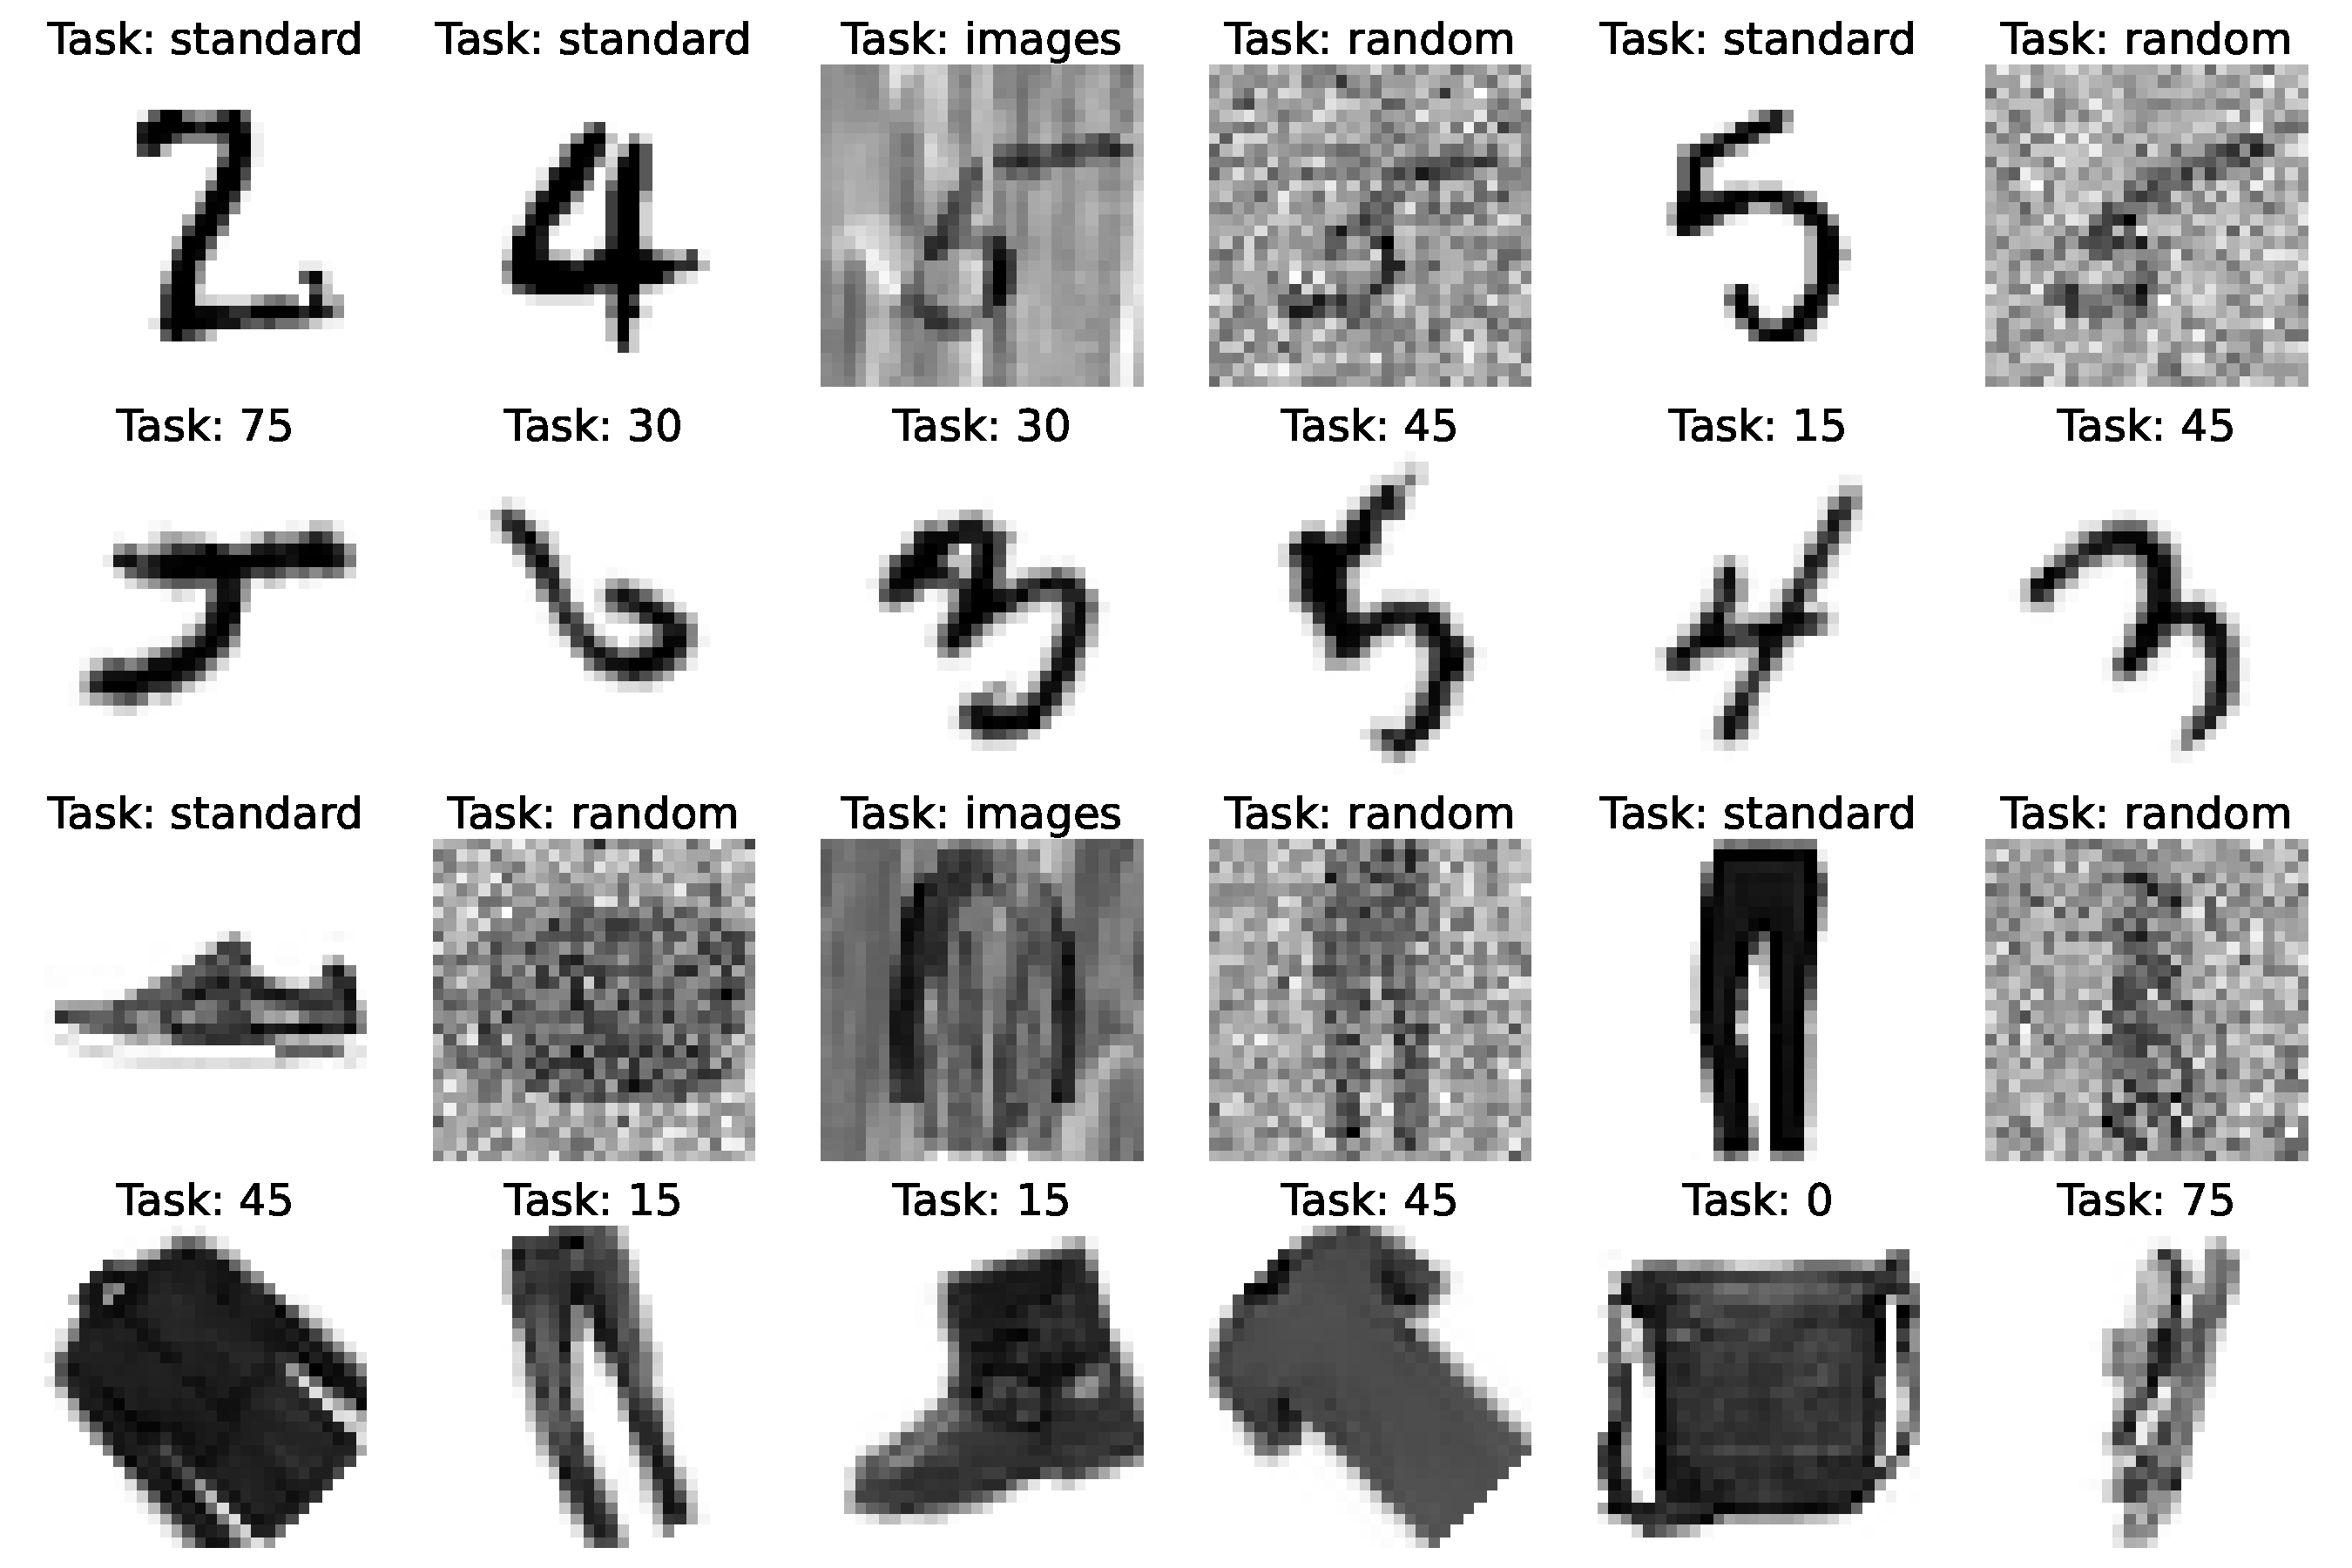
\includegraphics[width=\linewidth]{Chapter4/HAIS2022/hais22_datasets.pdf}
    \caption{Images of the four classification problems used. Each image has a title indicating the corresponding task. The rows correspond to \fdata{var-MNIST}, \fdata{rot-MNIST}, \fdata{var-FMNIST} and \fdata{rot-FMNIST} (from top to bottom).}
    \label{fig:problems_hais2022}
\end{figure}

\paragraph*{Problems Description.\\}
To test the Convex MTL neural networks we use four Multi-Task image datasets:
\fdata{var-MNIST}, \fdata{rot-MNIST}, based on MNIST~\citep{LeCunBBH98}, and \fdata{var-FMNIST}, \fdata{rot-FMNIST}, based on fashion-MNIST~\citep{xiao2017}.
%
The MNIST and fashion-MNIST datasets are both composed of \num{70000} examples of $28\times 28$ grey-scale images. The MNIST dataset contains images of handwritten numbers, while the fashion-MNIST has images of clothes and fashion-related objects.
Both are used as classification problems, where the images have to be classified in one of $10$ possible classes. These classes are balanced in both datasets.
%
To generate the Multi-Task image datasets that we use, we take the images from MNIST or fashion-MNIST and use either the \emph{variations} procedure or the \emph{rotation} one.

%
For the \fdata{var-MNIST} and \fdata{var-FMNIST} we use the \emph{variations} procedure. Inspired by the work of~\cite{BergstraB12}, we consider three transformations:
\begin{itemize}
    \item \textit{random}: adding random noise to the original image.
    \item \textit{image}: adding a random patch of another image to the original image.
    \item \textit{standard}: no transformations are applied to the original image.
\end{itemize}
Then, we use a random split to divide the original datasets in three groups. Each group is applied one of the transformations defined, so we get three tasks: two with \num{23333} examples and the third one with \num{23334}.

%
For the \fdata{rot-MNIST} and \fdata{rot-FMNIST} we use the \emph{rotations} procedure. Using the definitions of~\cite{GhifaryKZB15}, we consider six transformations:
\begin{itemize}
    \item \textit{0}: rotating $0^{\circ}$ the original image.
    \item \textit{15}: rotating $15^{\circ}$ the original image.
    \item \textit{30}: rotating $30^{\circ}$ the original image.
    \item \textit{45}: rotating $45^{\circ}$ the original image.
    \item \textit{60}: rotating $60^{\circ}$ the original image.
    \item \textit{75}: rotating $75^{\circ}$ the original image.
\end{itemize}
Again, we use a random split to divide the original datasets in six groups and each group is applied one of the transformations defined, so we get six tasks: four with \num{11667} examples and two with \num{11666}.
%

In Figure~\ref{fig:problems_hais2022} we show examples of the four MTL image problems that we generate, with the corresponding task annotation for each one.



\paragraph*{Experimental Procedure.\\}
% Models Considered
For testing the performance of our proposal we consider the following models:
\begin{itemize}
    \item \fmod{ctlNN}: a CTL-based neural network, that is, a single network for all tasks.
    \item \fmod{itlNN}: an ITL-based neural network, that is, an independent network for each task.
    \item \fmod{hsNN}: a MTL-based neural network using the hard sharing strategy. That is, a single neural network is used for all tasks, where the first layers are shared among tasks, but a task-specific output layer is used for each task.
    \item \fmod{cvxmtlNN}: a MTL-based neural network using the convex formulation we propose.
\end{itemize}
% convNet
All of these models are based on convolutional network, which we will name \fmod{convNet}, whose architecture is based on the Spatial Transformer Network~\citep{Jaderberg_2015} used in Pytorch\footnote{\href{www.pytorch.org/tutorials/intermediate/spatial\_transformer\_tutorial.html}{www.pytorch.org/tutorials/intermediate/spatial\_transformer\_tutorial.html}}.
The architecture of \fmod{convNet} consists, in this order, on two convolutional layers of kernel size $5$, with $10$ and $20$ output channels each; then a dropout layer, followed by a max pooling layer, and two hidden layers with $320$ and $50$ neurons. After this, the output layers follow.

%
In the \fmod{ctlNN}, we use a single network with the \fmod{convNet} architecture with $10$ output neurons, one for each class.
%
In the \fmod{itlNN}, an independent network, with the \fmod{convNet} architecture and $10$ output neurons, is used for each task.
%
For the \fmod{hsNN}, a single network with the \fmod{convNet} architecture is used, but we have a group of $10$ output neurons for each task in the problem. For example, if we are using of the \emph{rotation}-based problems, we would have $60$ output neurons, but only the group of $10$ corresponding to each task is used with each example.
%
In the \fmod{cvxmtlNN} we use a network with the \fmod{convNet} architecture and $10$ output neurons to model the common network and each of the task-specific networks. That is, given an example from task $r$, the $10$ common output neurons and the  $r$-th task-specific ones are combined to obtain the final output. 

% Optimizer and Hyperparameters
We use the AdamW algorithm~\citep{LoshchilovH19} to train all the models considered, and the weight decay parameter $\mu$ for each model is selected using a CV-based search over the values $\set{10^{-4}, 10^{-3}, 10^{-2}, 10^{-1}, 10^{0}}$. The rest of the parameters, which are part of the architecture, are fixed and set to the default values: the dropout rate is $0.5$ and we use a $2\times 2$ max pooling layer with a stride of $2$.
%
The \fmod{cvxmtlNN} model also has $\lambda$ as a hyperparameter, and it is selected, alongside $\mu$, using a CV grid search, where the grid for $\lambda$ is $\set{0, 0.2, 0.4, 0.6, 0.8, 1}$.

%
The train and test sets are generates using a task-stratified split of $70\%$ and $30\%$, respectively.
The CV grid searches are carried out using the training set, where we use a $5$-fold CV scheme. These folds are task-stratified, that is, all have the same task proportions. Also, since the problems are class-balanced and the sample size is reasonably large, the folds are expected to be class-balanceda as well.

\paragraph*{Results.\\}

\begin{table}[t!]
    \centering
        \caption{Test Accuracy with Majority Voting.}
        \label{tab:test_accuracy_majority}
    \begin{tabular}{l*{4}{c}}
        \hline
                           &   \fdata{var-MNIST} &   \fdata{rot-MNIST} &   \fdata{var-FMNIST} &   \fdata{rot-FMNIST} \\
        \hline
         \fmod{ctlNN} &              0.964 &           0.973 &                     0.784 &                  0.834 \\
         \fmod{itlNN} &              0.968 &           0.981 &                     0.795 &                  0.873 \\
         \fmod{hsNN}  &              0.971 &           0.980  &                    0.770  &                 0.852 \\
         \multirow{2}*{\fmod{cvxmtlNN}} &              \fmaxn{0.974} &           \fmaxn{0.984} &                     \fmaxn{0.812} &                  \fmaxn{0.880} \\
         & ($\lambda^* = {0.6}$)  & ($\lambda^* = {0.8}$) & ($\lambda^* = {0.6}$)  & ($\lambda^* = {0.6}$) \\
         \hline
        \end{tabular}
        
\end{table}

\begin{table}[t!]
    \centering
        \caption{Test Mean Categorical Cross Entropy.}
        \label{tab:test_crossentropy_mean}
    \begin{tabular}{l*{4}{c}}
        \hline
                           & \fdata{var-MNIST}   & \fdata{rot-MNIST}     & \fdata{var-FMNIST}   & \fdata{rot-FMNIST}   \\
        \hline
         \fmod{ctlNN} & 1.274 $\pm$ 0.143  & 1.145 $\pm$ 0.039 & 2.369 $\pm$ 0.183         & 1.757 $\pm$ 0.075      \\
         \fmod{itlNN} & 1.072 $\pm$ 0.029  & 0.873 $\pm$ 0.058 & 2.356 $\pm$ 0.130         & 1.598 $\pm$ 0.042      \\
         \fmod{hsNN}  & 1.087 $\pm$ 0.253  & 0.898 $\pm$ 0.073 & 3.067 $\pm$ 0.888         & 1.888 $\pm$ 0.075      \\
         \multirow{2}*{\fmod{cvxmtlNN}} & \fmaxn{0.924} $\pm$ \fmaxn{0.024}  & \fmaxn{0.831} $\pm$ \fmaxn{0.029} & \fmaxn{2.147} $\pm$ \fmaxn{0.090}         & \fmaxn{1.482} $\pm$ \fmaxn{0.063}      \\
         & ($\lambda^* = {0.6}$)  & ($\lambda^* = {0.8}$) & ($\lambda^* = {0.6}$)  & ($\lambda^* = {0.6}$)      \\
         \hline
        \end{tabular}
\end{table}

% Refitting models
To get more accurate results, less sensitive to randomness, we train each model $5$ different times. To do this, once the optimal hyperparameters have been selected using the CV in the training set, we refit the model with these hyperparameters using the whole training set. That is, the CV is done only once for each model in each problem, but then we repeat $5$ times the procedure of training the network over the whole training set.

% Accuracy vs Categorical CE
Although maximizing the accuracy is ultimately the goal in classification problems, it is not a differentiable measure, so we use the categorical cross entropy instead as the loss function to train the networks. Both measures are correlated, but they do not represent exactly the same behavior. We will show the results using both for completeness.

% Tables
Since we have $5$ instances of each model, a typical strategy to combine their predictions is majority voting. We perform this majority voting directly using the logits, in the output neurons, of each instance and averaging them, so we have $10$ values, one for each class.
In Table~\ref{tab:test_accuracy_majority} we show the test accuracy, using the logits average already described, for each of the approaches considered.
%
Other approach to visualize these results is to compute the categorical cross entropy directly on the averaged logits, which we show in Table~\ref{tab:test_crossentropy_mean}.
%
In both tables we also show the optimal values for $\lambda$ selected in the CV.

% Analysis
Our proposal, the \fmod{cvxmtlNN} model, obtains the best results in all the problems, either in terms of accuracy or cross entropy.
The ITL approach comes second in all problems, except for the accuracy score in \fdata{var-MNIST}, where the \fdata{hsNN} is second and \fdata{itlNN} goes third.
The \fdata{hsNN} model goes third in the rest of problems, while the \fdata{ctlNN} gets the worst results consistently in all problems, sometimes by a large margin.
%
By looking at the tables, it seems that a CTL approach is not able to capture the different properties of each task at once. On the other hand, the \fmod{ITL} approach obtains good results, because it is specialized in each task.
Considering the optimal values for $\lambda$, there are, however, common information shared among the tasks. These values fall far from the margins, so neither the CTL nor the ITL are optimal approaches. This is reflected in the tables, where the \fmod{cvxMTLNN} outperforms consistently \fmod{ctlNN} and \fmod{itlNN}. We can assume, then, that the information learned by the common network and the task-specific ones is complementary, because their combination lead to better results.
%
The hard sharing approach, although better than a CTL one, seems to be too rigid to effectively capture the differences among different tasks, so it is frequently surpassed by the ITL network.




% Complementing common and task-specific



\section{Application to Renewable Energy Prediction}\label{sec:convexmlt_renewable}

A transition towards renewable energies is taking place, with particular interest for solar and wind generation, which implies a demand for accurate energy production forecasts to be made for the transmission system operators, wind and solar farm managers and market agents. These forecasts can be made at different time horizons: very short (up to one hour), short (up to a few hours), or medium-long (one or more days ahead).
In this application of our convex MTL techniques to renewable energies forecast, we will focus wit the latter, in particular, the hourly, day-ahead prediction, that is, the prediction of tomorrow, at each hour, is predicted today.

Machine Learning (\acrshort{ml}), like in others forecasting problems, have an increasing presence in the energy prediction approaches. 
The usage of ML models require choosing the predictive features that will be used, which depends on the time horizon of interest. 
For short-term forecast, past values of energy production and real time meteorological data can be used; however, for longer horizons, the most common features are numerical weather predictions (\acrshort{nwp}), that can be provided by entities such as the \acrlong{ecmwf}, which is the one used in this work.
For the hourly day-ahead predictions of interest here, we use the NWP forecasts of the ECMWF run at \utc{00} in a given day to predict the hourly energy productions the day before. That is, using the NWP of \utc{00}, the energy generation predictions are given for each hour from {24} to {47}h.

After the selection of predictive features, the ML method better suited for the problem at hand has to be selected. Also, each method has a set of hyperparameters that influence on its behaviour and have to be adjusted in each case.
In the case of interest here, there are two possibilities: using local models for single installations or global models for multiple installations within a geographic area.

% Many ML approaches have been proposed for energy forecasting. 
% In the case of wind energy, prediction see, for example, the reviews of wind energy predictions of~\citep{giebel_soa,pinson2013,colak} or the application of concrete models to specific time-horizons~\citet{heinermann,zhu_genton}.
% For solar energy, we can see the surveys of~\citep{Antonanzas2016,Inman2013,Wan2015}, and a good reference for many aspects of photovoltaic energy can be found in~\cite{SEK}.

Anyway, any ML approach has to deal with the changing behaviour of a wind or solar farm, which can be altered substantially according to different conditions or time.
In the PV energy production this is obvious, since different times of the day, from sunrise to sunset, have very different behaviours; but there are also seasonal effects that affect the energy generation in the solar farms.
For wind energy, it is more difficult to define the variables that determine different scenarios. 
The energy velocity forecast is the most relevant variable for energy generation, but it is important to take into account the power curve of wind turbines, which has three different response zones: one for low speed and near zero production, an intermediate one with power growing with wind velocity and one with~maximum constant power up to the cut-off speed.
The angle in which this wind incide is also important, since the turbines of a farm have a specific direction. 
Finally, the assymetrical wind velocities between the day and night period can also affect the energy production.

One way to deal with this different behaviour scenarios is to apply a MTL model, where the models built are specialized in each scenario but all scenarios are used in the learning process.
In this Section a convex MTL approach will be used for wind and solar energy forecasting. To do this, it is necessary to define the tasks of interest on each case, which are described in the following subsections.
In the first subsection the experimental methodology is described, showing how the models are chosen and the hyperparameters are selected. Then, the next two subsection presents the approach and the detailed task definitions used for solar and wind energy, respectively, as well as the results to judge the resultant performance.

\subsection{Experimental~Methodology.\\}

%
\begin{table}[t!]
    \caption{Hyperparameters, grids used to find them (when appropriate), and hyperparameter selection method for each model. Here, $d$ is the number of {dimensions} % Please chang the font in the Table.
     of the data and $\sigma$ is the standard deviation of the~target.}
    \label{tab:hyperpars_grid_energies}
    \centering
     \begin{tabular}{*{5}{c}}
     \toprule
     \fhead{Par.} & \fhead{Grid} & \fhead{ctlSVR} & \fhead{itlSVR} & \fhead{cvxMTL} \\
     \midrule
      $C$ &  $\set{10^k: -1 \leq k \leq 6}$ & CV & CV & CV  \\
      $\epsilon$ & $\set{\frac{\sigma}{2^k}: 1 \leq k \leq 6}$ & CV & CV & CV  \\
      $\gamma$ & $\set{\frac{4^k}{d}: -2 \leq k \leq 3}$ & CV & - & ctlSVR \\
      $\gamma_r$ & $\set{\frac{4^k}{d}: -2 \leq k \leq 3}$ & - & CV & itlSVR\\
      $\lambda$ & $\set{10^{-1}k: 0 \leq k \leq 10}$ & - & - & CV \\
      \bottomrule
     \end{tabular}
\end{table}

Here we describe the methodology that we have followed to conduct the experiments of renewable energy prediction.
%
For the solar and wind energy we use the same procedure. In each problem, we have a train, validation and test sets, each corresponding to one year of data. In the solar energy problems we have 2013, 2014 and 2015 as train, validation and test sets, respectively; while for wind energy problems we use 2016, 2017 and 2018.
%
For both solar and wind problems we use different definition of tasks. To define these tasks we use only the training data, which partition the data, then, with these tasks' definition, we apply them to get the tasks of the validation and test examples.
%
For example, if we use the wind velocity to define three tasks, we study the velocities of the training examples to set the boundaries that define each task; then, we use this definitions on the validation and test sets.
%
We will represent the task definition applied with the nomenclature: \fmodt{taskDef}{modelName}, where \fmod{taskDef} is a name for the task definition and \fmod{modelName} is the name of the model.

%
We consider three different models based on the standard Gaussian kernel SVR:
\begin{itemize}
    \item \fmod{ctlSVR}: a CTL model, that is, a single SVR for all tasks. Its set of hyperparameters is $\set{C, \gamma, \epsilon}$, where $C$ is the regularization trade-off parameter, $\gamma$ is the kernel width, and $\epsilon$ the width of the error insensitive area.
    \item \fmod{itlSVR}: an ITL model, that is, an independent SVR for each task. For each task, we have standard SVR with its hyperparameters: $\set{C_r, \gamma_r, \epsilon_r}$ for $r=1, \ldots, \ntasks$.
    \item \fmod{mtlSVR}: a convex MTL model, as shown in Subsection~\ref{subsec:cvx_l1-svm}, with its corresponding set of hyperparameters is $\set{C, \epsilon, \gamma, \gamma_1, \ldots, \gamma_\ntasks, \lambda_1, \ldots, \lambda_\ntasks}$, where $\gamma$ is the kernel width of the common part and $\gamma_r$ the one of the $r$-th specific part; also, $\lambda_r$ is the convex combination parameter corresponding to the $r$-th task.
\end{itemize}
%
Although the CTL approach does not use the tasks information, the ITL and MTL models depend on the task definition that we use. For example, prediction at different hours can define different tasks, where the possible values are, for example, (\fmod{hour}=14) or (\fmod{hour}=12). The models using this task definition will be named \fmodt{hour}{itlSVR} and \fmodt{hour}{mtlSVR}. 
%
Since each task definition partition the data, we can also use multiple task definitions, combining them and creating finer partitions. 
We will name \fmod{(taskDef1,...,taskDefM)} the combination of task definitions \fmod{taskDef1}, ..., \fmod{taskDefM}. For example, consider the \fmod{(hour)} definition, which, in our definition consider 14 different hours, hence, 14 tasks; and consider the \fmod{season} definition, which considers the prediction in each season as a different task, hence, four tasks. The combined definition \fmod{(hour, season)} generates $14 \times 4$ possible tasks, whose values can be, for example, \fmod{(hour = 12, season = summer)}.
The models using this combination will be named \fmodt{hour, season}{itlSVR} or \fmodt{hour, season}{mtlSVR}.

%
As explained in Subsection~\ref{subsec:cvx_l1-svm}, the cost of methods to select the optimal hyperparameters scale exponentially with the dimension, so it is not feasible to use a CV grid search, for example, if we have more than $3$ hyperparameters.
%
In the \fmod{ctlSVR} and \fmod{itlSVR} it is not a problem, since we have $3$ hyperparameters, for the common, single SVR, and for the task-independent ones, respectively. We use then a CV grid search, using as train and validation sets described above.
However, to find the hyperparameters of \fmod{mtlSVR} we have to make some adjustements, as shown in Subsection~\ref{subsec:convexmtlsvm_exp}. 
%
First, we use a convex MTL formulation with a single $\lambda$ parameter, common to all tasks.
%
Second, we use the optimal kernel widths selected in validation for the CTL and ITL approaches as the widths in the MTL approach. That is, we get the optimal common $\gamma^*$ and task-specific $\gamma^*_1, \ldots, \gamma^*_\ntasks$, and fix them in the \fmod{mtlSVR} model, not including them in the grid search procedure.
Then, we use a CV grid search to find the optimal values of the remaining hyperparameters, that is, $\set{C, \epsilon, \lambda}$.
%
In Table~\ref{tab:hyperpars_grid_energies} we show the method to obtain each hyperparameter, as well as the grids used in the CV grid search procedures.
We use the \acrshort{mae} as the validation metric, because is the most natural to the $\epsilon$-insensitive loss that is used in the SVRs.

%
The whole procedure to get the final scores is:
\begin{enumerate}
    \item \textbf{Scaling the target and normalizing the features.} We scale the target values to $[0, 1]$ and we normalize each feature, so it has $0$ mean and a standard deviation of $1$. This is done using the training data only. 
    For the target scale, we select the target minimum and maximum values of the training set, that is, $y_\text{min} = 0$, when no energy is produced, and $y_\text{max}$ is the maximum capacity of the park.    
    %Then, the target in train, validation and test sets is normalized as     $y_\text{scaled} = (y - y^\text{tr}_\text{min}) / (y^\text{tr}_\text{max} - y^\text{tr}_\text{min} )$.
    %For example, for feature normalization, we compute the training mean $\mu_d^\text{tr}$ and standard deviation $\sigma_d^\text{tr}$ of feature $d$, then we normalize the corresponding feature in the whole dataset using $\hat{X}_d = (\hat{X}_d - \mu_d^\text{tr}) /  \sigma_d^\text{tr}$.
    \item \textbf{Using a CV grid search to select the optimal hyperparameters.} This is done using the train and validation sets, with the grids and adjustements already explained. We use the MAE as our validation metric.
    \item \textbf{Predict on the test set and rescale to the original scale.} That is, we use the corresponding model $f(\cdot)$ to compute the prediction of the normalized $i$-th test example from task $r$, $\tilde{x}_i^r$, as $f(\tilde{x}_i^r)$. Then, we rescale it back to obtain the final prediction $\hat{y}_i^r = f(x_i^r) \times (y_\text{max} - y_\text{min} ) + y_\text{min}$
    \item \textbf{Compute the test score.} Using the target values $y_i^r$ and their corresponding predictions, $\hat{y}_i^r$, we measure the performance of our model using both MAE and MSE.
\end{enumerate}
The whole process is carried out using a \fcode{Pipeline} object, where we make use of class \fcode{StandardScaler} to normalize the data, and \fcode{TransformedTargetRegressor} class to scale the targets. All these classes are part of the \emph{scikit-learn} library.

%
To put our results in perspective, we also show the errors of simple persistence models and of multilayer perceptrons. For the perceptron we use the \fcode{MLPRegressor} class of \emph{scikit-learn}. The architecture for both problems consists on fully connected networks with two hidden layers, with $100$ and $50$ neurons. We train these networks using the L-BFGS solver with a maximum of $800$ iterations a tolerance of $10^{-10}$. The regularization hyperparameter is selected using a CV grid search, as those described above, where the grid is $\set{4^k: -2 \leq j \leq 3}$.






\subsection{Solar Energy}
The goal is to predict the hourly energy production in two parks, located in the islands of Majorca and Tenerife, and name the corresponding problems as \fdata{majorca} and \fdata{tenerife}, respectively. 
%
In this subsection the experiments with these solar problems are presented, using the experimental procedure already shown. First a description of the problems is given and the data used, then the results are given and analyzed.

\paragraph*{Data and~Tasks.\\}
For both problems, \fdata{majorca} and \fdata{tenerife}, the same variables, extracted from the Numerical Weather Prediction (NWP), are used. These variables, extracted from NWP predictions made by the European Center for Medium Weather Forecasts 
(ECMWF;~\cite{ECMWF}), are:
\begin{itemize}
    \item Surface net solar {radiation} (\ftt{SSR}).
    \item Surface solar radiation {downwards} (\ftt{SSRD}).
    \item {Total Cloud Cover} %Please change it not to be captitalized if unnecessary.
     (\ftt{TCC}).
    \item Temperature at 2 {meters} (\ftt{T2M}).
    \item Module of the speed of wind at {10 meters} (\ftt{v10}).
\end{itemize}
The radiation variables \ftt{SSR}, solar radiation, and \ftt{SSRD}, solar radiation plus the diffuse radiation scattered by the atmosphere, as well as the \ftt{TCC}, have all a direct impact on PV production.
%
The \ftt{T2M} and \ftt{v10} features are also considered because they influence the conversion of photon energy into electrical one, and also the overall performance of PV stations.
%

To collect these features, geographical grids with a $\ang{0.125}$ spatial resolution are considered. For \fdata{majorca}, the grid has its northeast coordinates at $(\ang{2}, \ang{40})$, and its southwest coordinates at $(\ang{4}, \ang{39})$. For \fdata{tenerife}, the coordinates are $(\ang{-17.5}, \ang{28.75})$ for the northeast corner, and $(\ang{-15.5}, \ang{27.75})$ for the southwest one.
%
That is, both grids have a longitude width of 2 degrees and a latitude height of 1 degree. With the spatial resolution considered, this results in a total number of $17 \times 9 = 153$ grid points; since we use five variables at every point, the total dimension of our data is thus $5 \times 153 = 765$. 


%
Observe that we obtain large dimensional patterns, where the features might be highly correlated. That is, a feature, \ftt{SSR} for example, measured in one point of the grid and another close point might be very correlated, since the grids are squares with sides of about $\km{12}$.
This correlation will affect those models based on matrix-vector computations, such as linear models, which are the most obvious, but, also, to some extent, to neural networks.
Although Ridge or Tikhonov regularization can alleviate this issue for these models, the kernel-methods, such as the kernel SVMs, seems better suited for these kind of problems.
When we use kernel methods, such as the Gaussian kernel $\exp{-\gamma \norm{x-y}^2}$, the algorithm learns using the distances among patterns $\norm{x - y}$, instead of its features.
%
These distances scale linearly with the dimension of data, that is, consider the features scaled to $[0, 1]$, then a rough estimate of the distance between two patterns would be $d$. In the extreme case where all features are equal, i.e. $x_j = x_1$ for all $j=1, \ldots, \dimx$; then, $\norm{x - x'} = d(x_1 - {x'}_1)$.
However, this influence of the dimension can be easily controlled by $\gamma$, and, if selected properly, should not affect the performance of a Gaussian SVR.

%
Recall that we use data from years 2013, 2014 and 2015 as train, validation and test sets, respectively.
%
We show the errors in both total \mwhu{} and as percentages, in the range $[0, 100]$ of the total install PV power in each photovoltaic park, {\mw{72.46}} in \fdata{majorca} and \mw{107.68} in \fdata{tenerife}.
%
We remove night data for obvious reasons and make predictions between \utc{06} and \utc{19} {for} \fcode{majorca} and between \utc{07} and \utc{20} for \fcode{tenerife}.
%
The hour of the day has a direct influence on the solar radiation, and, therefore, on energy production. Also, the season of the year has a similar impact on the production. This leads to two obvious task definitions:
\begin{itemize}
    \item	\fcode{hour}: The prediction at each hour is defined as a different task; there are thus 14 tasks in \fcode{majorca} (from 06 to \utc{19}) and \fcode{tenerife} (from 07 to \utc{20}).
    %We observe in Figures~\ref{fig:maj_groupby_hour} and~\ref{fig:ten_groupby_hour} that the distribution of the target, i.e.,~the photovoltaic energy, is very dependent on the hour chosen.
    \item	\fcode{season}: The prediction at each season is defined as different task.  With~a slight abuse of language, the definitions for each season used are: Spring, from~16 February to 15 May; Summer, from~16 May to 15 August; Autumn, from~16~August to 15 November; and~Winter, from~16 November to 15 February.
    %We can observe in Figures~\ref{fig:maj_groupby_season} and~\ref{fig:ten_groupby_season} that different seasons have different means of the target.
\end{itemize}
%
In Subfigures~\ref{fig:maj_groupby_hour} and~\ref{fig:ten_groupby_hour} the hourly averages of the PV energy in \mwhu{} are shown for \fdata{majorca} and \fdata{tenerife}.
Also, in Subfigures~\ref{fig:maj_groupby_season} and~\ref{fig:ten_groupby_season} the monthly averages, colored by season.
\begin{figure}[H]
    \centering%
    \subfloat[][]{%    
    \includegraphics[width=.35 \textwidth]{Chapter4/energies/majorca_groupby_hour_train.pdf}
    \label{fig:maj_groupby_hour}}\quad%
    \subfloat[][]{%
    \includegraphics[width=.35 \textwidth]{Chapter4/energies/tenerife_groupby_hour_train.pdf}
    \label{fig:ten_groupby_hour}}\\
    \subfloat[][]{%
    \includegraphics[width=.35 \textwidth]{Chapter4/energies/hist_season_majorca_train_byMonth.pdf}
    \label{fig:maj_groupby_season}}\quad%
    \subfloat[][]{%
    \includegraphics[width=.35 \textwidth]{Chapter4/energies/hist_season_tenerife_train_byMonth.pdf}
    \label{fig:ten_groupby_season}}
 \caption{\label{fig:solar_task_def}Hourly photovoltaic energy mean {in} \fcode{majorca}~\protect\subref{fig:maj_groupby_hour} {and}~\fcode{tenerife}~\protect\subref{fig:ten_groupby_hour} measured in \mwhu{}. Photovoltaic energy monthly averages for \fcode{majorca}~\protect\subref{fig:maj_groupby_season} and \fcode{tenerife}~\protect\subref{fig:ten_groupby_season} , colored using the tasks defined using the season and measured in \mwhu{}. All the histograms have been computed using data from year~2016.}
 \end{figure}
 




\paragraph*{Experimental~Results.\\}

\begin{table}[H]
    \caption{Test MAEs (left), test MSEs (center), and optimal mixing $\lambda^*$ (right) of the solar energy models considered {in} \fcode{majorca}. {Base units} %Is the bold in the Table necessary? If is not necessary, please remove it. Also, please remove the font in the table. Same as below.
     are either \mwhu{} or percentages (\%). The~best model errors are shown in~bold.}
    \centering
    \label{table:solar_scores_m}
 \begin{tabular}{lccccccc}
    \toprule
     & \fheadmulti{3}{MAE} & \fheadmulti{3}{MSE} & \fhead{$\lambda^*$}\\
    & {{\mwhu}}	& {{\%}} & {rank} & {{\mwhu}}	& {{\textpertenthousand}} & {Rank}& \\
    \midrule
    \fmod{ctlSVR}    &  5.265 &  7.265  & (6) &  59.322 &  112.985  & (6) &  - \\
    \fmod{(season)\_itlSVR}   &  5.305 &  7.384  & (7) &  59.591 &  113.498  & (7) &  - \\
    \fmod{(season)\_mtlSVR}   &  \fmaxn{4.884} &  \fmaxn{6.740}  & \fmaxn{(1)} &  53.222 &  101.366  & (2) &  0.4 \\
    \fmod{(hour)\_itlSVR}   &  5.083 &  7.015  & (4) &  54.540 &  103.877  & (3) &  - \\
    \fmod{(hour)\_mtlSVR}   &  4.957 &  6.840  & (2) &  \fmaxn{52.614} &  \fmaxn{100.208}  & \fmaxn{(1)} &  0.3 \\
    \fmod{(hour, season)\_itlSVR}   &  5.250 &  7.251  & (5) &  57.927 &  110.328  & (5) &  - \\
    \fmod{(hour, season)\_mtlSVR}   &  5.038 &  6.952  & (3) &  54.601 &  103.992  & (4) &  0.3 \\
    \bottomrule
    \end{tabular}
 \end{table}
\unskip


 \begin{table}[H]
    \caption{Test MAEs (left), test MSEs (center), and optimal mixing $\lambda^*$ (right) of the solar energy models considered {in} \fcode{tenerife}. Base units are either \mwhu{} or percentages (\%). The~best model errors are shown in~bold. The positions with hyphens correspond to the model ranked first in terms of MAE or MSE, as indicated by its column.}
    \centering
    \label{table:solar_scores_t}
 \begin{tabular}{lccccccc}
    \toprule
     & \fheadmulti{3}{MAE} & \fheadmulti{3}{MSE} & \fhead{$\lambda^*$}\\
    & {{\mwhu}}	& {{\%}} & {Rank} & {{\mwhu}}	& {{\textpertenthousand}} & {Rank}& \\
    \midrule
    \fmod{ctlSVR}    &  5.786 &  5.373  & (5) &   88.323 &  76.174  & (5) &  - \\
    \fmod{(season)\_itlSVR}   &  5.930 &  5.545  & (6) &   97.454 &  84.611  & (6) &  - \\
    \fmod{(season)\_mtlSVR}   &  5.579 &  5.181  & (4) &   86.227 &  74.366  & (3) &  0.8 \\
    \fmod{(hour)\_itlSVR}   &  5.403 &  5.018  & (2) &   86.686 &  74.762  & (4) &  - \\
    \fmod{(hour)\_mtlSVR}   &  \fmaxn{5.376} &  \fmaxn{4.993}  & \fmaxn{(1)} &   \fmaxn{84.207} &  \fmaxn{72.624}  & \fmaxn{(1)} &  0.7 \\
    \fmod{(hour, season)\_itlSVR}   &  6.025 &  5.554  & (7) &  104.536 &  90.297  & (7) &  - \\
    \fmod{(hour, season)\_mtlSVR}   &  5.494 &  5.102  & (3) &   85.440 &  73.687  & (2) &  0.7 \\
    \bottomrule
    \end{tabular}
 \end{table}
\unskip


\begin{table}[H]
   \caption{Wilcoxon $p$-values for absolute (left) and quadratic (right) errors.}
   \centering
   \label{table:solar_wilcoxon}
   %% \tablesize{} %% You can specify the fontsize here, e.g.,~\tablesize{\footnotesize}. If commented out \small will be used. Is the bold necessary. Same as others in the table.
   \begin{tabular}{lcccc}
      \toprule
      & \fheadmulti{2}{MAE} &  \fheadmulti{2}{MSE}\\
      & {\fcode{majorca}}	& {\fcode{tenerife}} & {\fcode{majorca}}	& {\fcode{tenerife}}\\
      \midrule
   \fmod{ctlSVR}                           &    0.014 (4) &    0.000 (5) &    0.081 (4) &    0.000 (5) \\
   \fmod{(season)\_itlSVR}                &    0.008 (5) &    0.636 (5) &    0.215 (4) &    0.354 (5) \\
   \fmod{(season)\_mtlSVR}         &   ------ %MDPI: We changed it into minus, please confirm.
{(1)} &    0.000 (4) &    0.036 (2) &    0.000 (3) \\
   \fmod{(hour)\_itlSVR}                  &    0.693 (2) &    0.006 (2) &    0.000 (3) &    0.000 (4) \\
   \fmod{(hour)\_mtlSVR}           &    0.067 (1) &   ------ {(1)} &   ------ {(1)} &   ------ {(1)} \\
   \fmod{(hour, season)\_itlSVR}        &    0.000 (3) &    0.000 (6) &    0.000 (4) &    0.098 (5) \\
   \fmod{(hour, season)\_mtlSVR} &    0.000 (2) &    0.000 (3) &    0.745 (3) &    0.000 (2) \\
   \bottomrule
\end{tabular}
\end{table}

In Tables~\ref{table:solar_scores_m} and~\ref{table:solar_scores_t} we show the numerical results for \fdata{majorca} and \fdata{tenerife}, respectively. We give the test MAE, which is the most natural metric for SVRs, as well as the MSE. 
In the case of percentages, for MAE, we give the percentage corresponding to the total installed power, and for the MSE, the permyriad, that is per \num{10000}, of the installed power.
%
We also show the rankings in terms of MAE or MSE, and the optimal hyperparameter $\lambda^*$ selected in the CV for the MTL models.
%

To show statistical significance the Wilcoxon test is used, but instead of testing every pair of models, the rankings of Tables~\ref{table:solar_scores_m} and~\ref{table:solar_scores_t} are used. The Wilcoxon test is applied between each model and the next in ranking at the $0.05$ level, to determine if the difference is significant.
The test is applied over the list of errors commited by each model in the patterns of the test set. When the null hypothesis of the Wilcoxon test is refused, it implies that the distribution of the difference between the errors does not have its median at $0$.
In Table~\ref{table:solar_wilcoxon}, we show the $p$-values of the pairwise tests. If the $p$-value is smaller than the level considered level of 0.05, then the different between models is considered significant.
%
With these procedure, a new significant ranking, shown in Table~\ref{table:solar_wilcoxon},  is generated: starting from the best model, we compare each model with the next best one, and we increase the ranking only if the difference is significant.
%
For example, in Table~\ref{table:solar_scores_m}, in terms of MAE, the first model, \fmod{(season)\_mtlSVR}, is tested against the second one, \fmod{(hour)\_mtlSVR}. In Table~\ref{table:solar_wilcoxon}, we show the $p$-value corresponding to that test, which is $0.067$, and since it is larger than the level $0.05$, the ranking is not increased and both models have the same significant ranking. 

%
Looking at the tables, it is easy to see that the MTL approaches obtain the best results in both problems, while \fmod{ctlSVR} has the worst performance in \fcode{tenerife} and second worst in \fcode{majorca}.
ITL models are more difficult to interpret, although they are always behind their corresponding MTL approaches, they can obtain good results, like the \fmodt{hour}{itlSVR} in \fdata{majorca} which is second; but they can also have bad performances, like the \fmodt{season}{itlSVR} in \fdata{tenerife}.

%
The $\lambda^*$ values can help to understand this behaviour. In both problems, the selected values lie far from the extremes $0$ or $1$, which distances the MTL approaches from the CTL or ITL ones. If these values are optimal, then the CTL or ITL equivalent models, with $\lambda=1$ and $\lambda=0$, respectively, obtain a worse result in validation. This is reflected also in the test set, as shown in the tables.
Also, it is noticeable that the optimal values for \fdata{majorca} are all smaller than $0.5$, which can be intepreted as models with a stronger common part, while in \fdata{tenerife}, the optimal values are larger than $0.5$ which reflects stronger independent parts.
%
Although the MTL approaches get the best results with any task definition, the \fmod{(hour)} definition seems to work best than the \fmod{(season)} one. The \fmodt{hour}{mtlSVR} gets a second best result, which is not significantly worse than the best one in \fdata{majorca}, and the single best result in \fdata{tenerife}.

%
For completeness the scores of persistence models and a neural network are given.
The persistence forecasts are obtained by predicting at each hour the target value 24 hours prior. By doing this, the MAE scores for majorca are \mwh{5.776} and \mwh{7.766}, which scaled to $[0, 100]$ correspond to 7.97\% and 7.21\%; which are an 18\% and 44\% error increase of the best MTL models.
The neural network errors are \mwh{5.140} and \mwh{5.763}, that is, 7.09\% and 5.35\% of the total PV installed. While this results are still competitive, this performance is worse than those of the convex MTL models proposed.


\begin{figure}[H]
    \centering%
    \subfloat[]{%
    \includegraphics[width=.3 \textwidth, height=.3 \textwidth]{Chapter4/energies/best_ctl_majorca.pdf}
    \label{fig:best_ctl_majorca}}\quad%
    \subfloat[]{%
    \includegraphics[width=.3 \textwidth, height=.3 \textwidth]{Chapter4/energies/best_itl_majorca.pdf}
    \label{fig:best_itl_majorca}}\quad%
    \subfloat[]{%
    \includegraphics[width=.3 \textwidth, height=.3 \textwidth]{Chapter4/energies/best_mtl_majorca.pdf}
    \label{fig:best_mtl_majorca}}\\
 \caption{\label{fig:majorca_best_plots} Real energy production against prediction made by the best CTL~\protect\subref{fig:best_ctl_majorca}, ITL~\protect\subref{fig:best_itl_majorca}, and MTL~\protect\subref{fig:best_mtl_majorca} models {in} \fcode{majorca} in terms of MAE; the perfect prediction line is shown in orange. The~units of the axis are \mwhu{}.}
\end{figure}

\begin{figure}[H]
    \centering%
    \subfloat[]{%
    \includegraphics[width=.3 \textwidth, height=.3 \textwidth]{Chapter4/energies/best_ctl_tenerife.pdf}
    \label{fig:best_ctl_tenerife}}\quad%
    \subfloat[]{%
    \includegraphics[width=.3 \textwidth, height=.3 \textwidth]{Chapter4/energies/best_itl_tenerife.pdf}
    \label{fig:best_itl_tenerife}}\quad%
    \subfloat[]{%
    \includegraphics[width=.3 \textwidth, height=.3 \textwidth]{Chapter4/energies/best_mtl_tenerife.pdf}
    \label{fig:best_mtl_tenerife}}\\
 \caption{\label{fig:tenerife_best_plots} Real energy production against prediction made by the best CTL~\protect\subref{fig:best_ctl_tenerife}, ITL~\protect\subref{fig:best_itl_tenerife}, and MTL~\protect\subref{fig:best_mtl_tenerife} models {in} \fcode{tenerife} in terms of MAE; the perfect prediction  line is shown in orange. The~units of the axis are \mwhu{}.}
\end{figure}


%
To get a better understanding of the results we plot the predictions against the target values of the CTL model and the best ITL and MTL ones.
%
In the case of \fdata{majorca}, we plot the predictions \fmod{ctlSVR}, \fmodt{hour}{itlSVR} and \fmodt{season}{mtlSVR} in Figure~\ref{fig:majorca_best_plots}.
From these scatter plots it seems that the CTL approach has a larger deviation in its predictions, while the ITL one has a bias, that is, it systematically underestimates the prediction corresponding to larger values of energy production.
The MTL approach seems to correct, to a certain degree, this bias of the ITL model, while preserving a smaller variance than the CTL one.
%
For \fdata{tenerife} we plot the predictions of \fmod{ctlSVR}, \fmodt{hour}{itlSVR} and \fmodt{hour}{mtlSVR}, which are shown in Figure~\ref{fig:tenerife_best_plots}.
It is more difficult to interpret the plots in this case, although it is possible to highlight that the MTL approach seems less prone to overestimate the production at lower values than either the CTL or ITL models.








\subsection{Wind Energy}

\paragraph*{Data and~Tasks.\\}

\begin{figure}[H]
    \centering%
    \subfloat[]{%
    \includegraphics[width=.38 \textwidth]{Chapter4/energies/polarhist_tasks_angle_stv_train.pdf}
    \label{fig:stv_task_angle}}\quad%
    \subfloat[]{%
    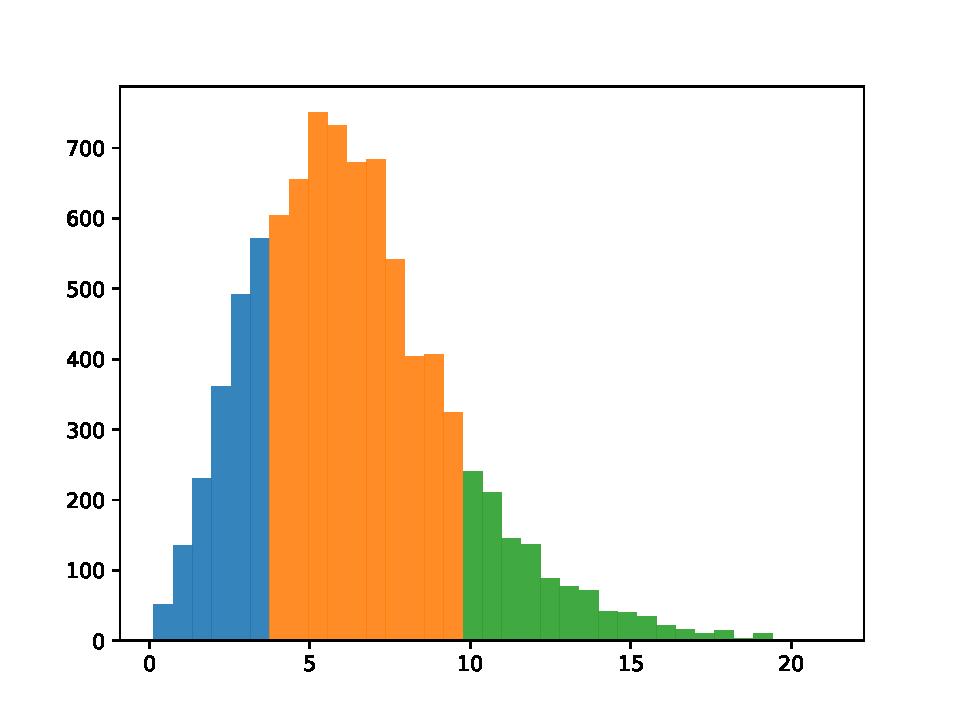
\includegraphics[width=.38 \textwidth]{Chapter4/energies/hist_tasks_velocity_stv_train.pdf}
    \label{fig:stv_task_velocity}}\\
 \caption{\label{fig:wind_task_def} Histograms of wind. ~\protect\subref{fig:stv_task_angle} {Histogram} %Please add figure caption. For example. Figure 4. xxxx (a)xxxx (b)xxxxxx.
  of wind angles derived from NWP data for the year 2016 in Sotavento colored by task \fmod{angle}. ~\protect\subref{fig:stv_task_velocity}  Histogram of wind velocity derived from NWP data for the year 2016 and measured in m/s in Sotavento colored by {task} \fmod{velocity}.}
\end{figure}

 \begin{figure}[H]
   \centering
   \subfloat[]{%
   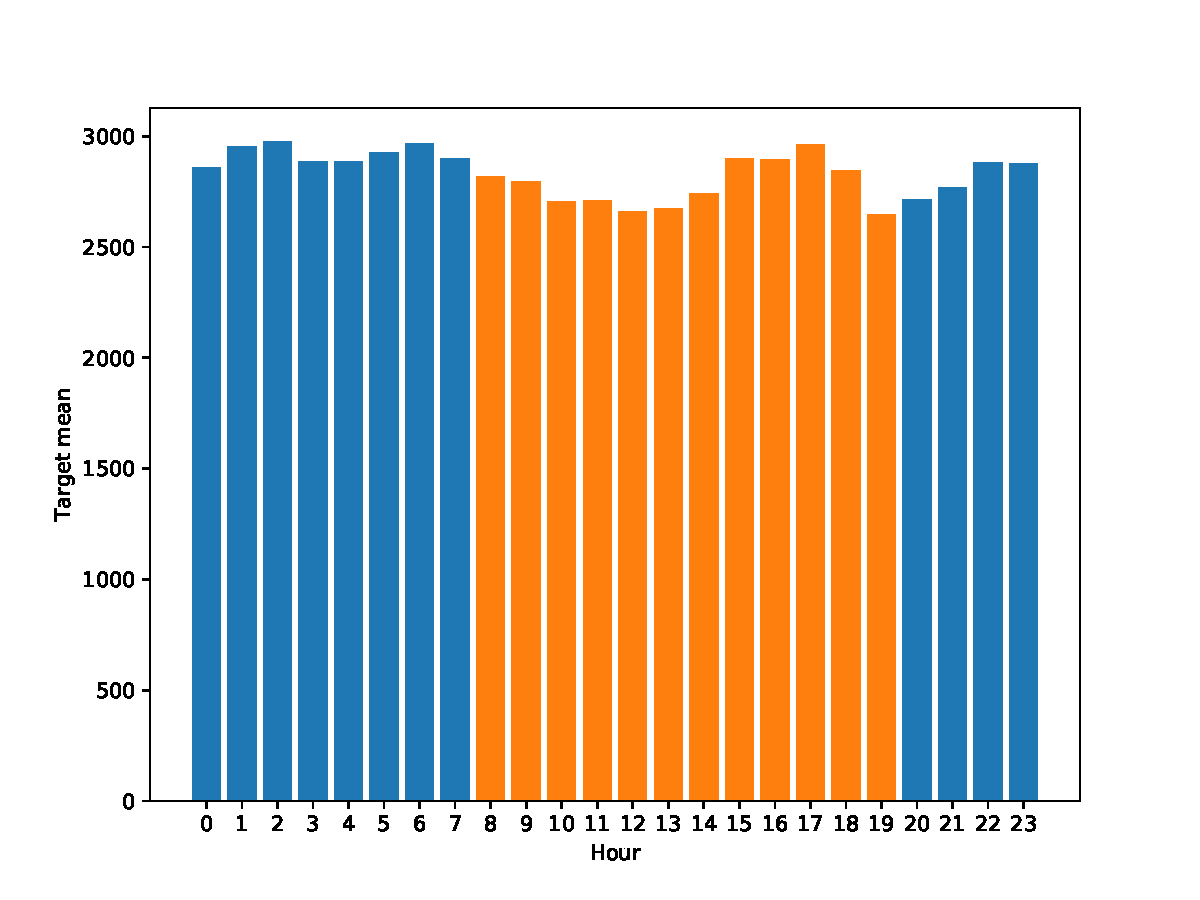
\includegraphics[width=.45 \textwidth]{Chapter4/energies/hist_timeOfDay_stv_train_byHour.pdf}
   \label{fig:hist_timeOfDay_stv_target}}%
\subfloat[]{%
    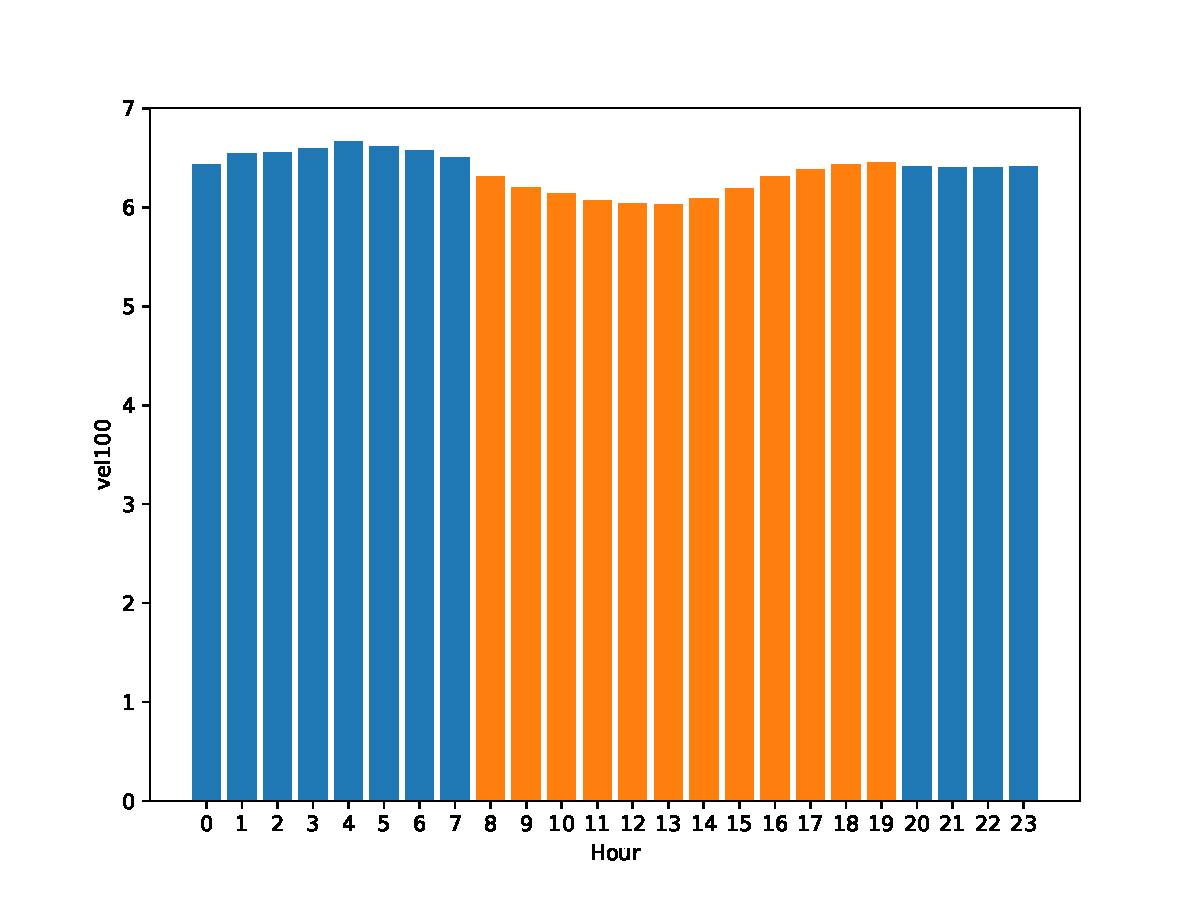
\includegraphics[width=.45 \textwidth]{Chapter4/energies/hist_timeOfDay_stv_vel100_byHour.pdf}
    \label{fig:hist_timeOfDay_stv_vel100}}
% \hspace{\fill}
\caption{\label{fig:wind_task_def_tday} Histograms of wind. ~\protect\subref{fig:hist_timeOfDay_stv_target} {Hourly mean measured} %Please add figure caption. For example. Figure 5. xxxxx (a)xxxxx (b)xxxx. In addition, is it necessary to add explanations of different color cylinders?
 in \si{\kilo{\watt\hour}} of generated energy during the year 2016 in Sotavento colored by {task} \fmod{timeOfDay}. ~\protect\subref{fig:hist_timeOfDay_stv_vel100} Hourly mean of velocity in Sotavento derived from NWP data for the year 2016 and measured in m/s at \SI{100}{\metre} colored by {task} \fmod{timeOfDay}.}
\end{figure}

\begin{figure}[H]
   \centering
   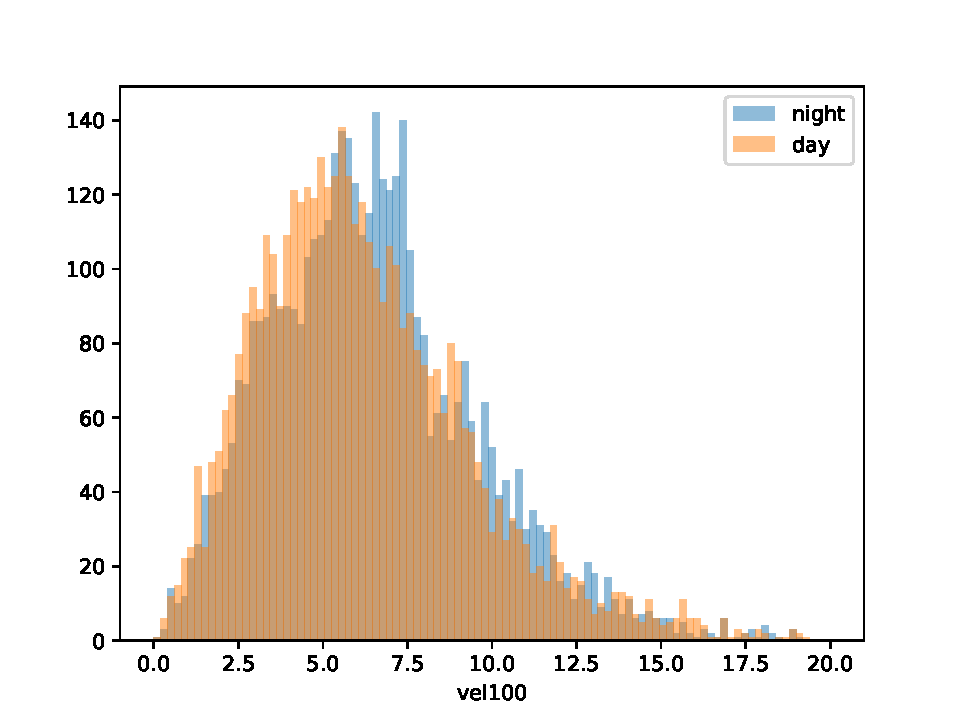
\includegraphics[width=.5\textwidth]{Chapter4/energies/hist_timeOfDay_stv_vel100_normal.pdf}
 \caption{\label{fig:stv_vel100} Histograms of the velocity of wind at 100m derived from NWP data for the year 2016 and measured in m/s during the day and night in Sotavento.
%  \comm{decir para qué año. Hay una cosa que no entiendo: a ojo parece que hay más datos de night que de day, lo que no debería ser. Pero mirando la fig anterior hay 11 horas night-azul- y 13 day naranja. Claramente está mal, pero así las cosas los colores de abajo están al revés}
}
\end{figure}

We want to predict the wind energy production at the Sotavento wind park located in Galicia, Spain. The variables from the NWP that we consider as predictors are:
\begin{itemize}
    \item	Eastward component of the wind at {10 m} %Please remove the font. Same as below
     (\ftt{U10}).
    \item	Northward  component of the wind at {10 m} (\ftt{V10}).
    \item   Module of velocity of the wind at 10 m.
    \item	Eastward  component of the wind at {100 m} (\ftt{U100}).
    \item	Northward component of the wind at {100 m} (\ftt{V100}).
    \item   Module of velocity of the wind at 100 m.
    \item   Surface {Pressure} (\ftt{sp}).
    \item	2 meter {temperature} (\ftt{2t})
\end{itemize}
These variables are collected in a grid, which is approximately centered at the farm, with northeast and southwest coordinates at $(\ang{-9.5}, \ang{44})$ and $(\ang{-6}, \ang{42.25})$, respectively, and a spatial resolution of $\ang{0.125}$.
This results in a grid with $435$ points, that, with the $8$ variables considered at each point, gives a total number of {3480} predictive features.
We scale the energy productions values to $[0, 100]$ using the maximum power installed (\mw{17.56}), which corresponds to the value $100$.
%
Recall that we have three years of data: 2016, 2017 and 2018, which are used as train, validation and test sets.
%
Although there are no obvious task definitions, we consider three different criteria:
\begin{itemize}
    \item \fmod{angle}: Here the wind angle at a height of $100m$ is considered, which is obtained from the \ftt{U100} and \ftt{V100} variables. 
    First, the most frequent angle is estimated, which is $\ang{56}$, and then, we use it as the center of the first quadrant. That is, the patterns that correspond to the first task as those whose wind angle lies between ${11}$ and $\ang{101}$  The other three quadrants, corresponding to a task each, are defined by the remaining sectors of $\ang{90}$.
    The histogram of wind angles, and the defined quadrants in different colors, are shown in Figure~\ref{fig:stv_task_angle}
    \item \fmod{velocity}: Here the wind velocity at a height of $100m$ is considered, which is again obtained from the \ftt{U100} and \ftt{V100} variables. The speed boundaries selected to define three tasks are $4$ and $10$m/s, which, for an ideal generator, are approximately the starting point of wind energy generation and its maximum power plateau, before cut-off speed.   
    In Figure~\ref{fig:stv_task_velocity} the histrogram of velocities is shown with the task regions colored. 
    \item \fmod{timeOfDay}: Here the 24 hours of a day are divided in two 12 hours periods: a day period between 08 and \utc{19}, and~a night one between 20 to \utc{07}.
    In Figures~\ref{fig:hist_timeOfDay_stv_target} and~\ref{fig:hist_timeOfDay_stv_vel100} the hourly average energy production and wind speed are shown, with the hours colored according to the two tasks defined. In Figure~\ref{fig:stv_vel100} the histograms of wind velocity in the night and day periods are shown.
\end{itemize}
%
For these task definitions, it is necessary to perform an analysis of the data, which is done only using the train set, corresponding to 2016.
The tasks in this case are not as clear as that defined for the solar energy. For the \fmod{angle} and \fmod{velocity} definitions some differences across tasks in the histograms can be found, but not definitive ones.
For the \fmod{timeOfDay} definition, the two histograms of Figure~\ref{fig:stv_vel100} look very similar.
Moreover, the boundaries of the tasks are set in a way that is partially arbitrary, and a bad selection of tasks could lead to poor results.


\paragraph*{Experimental~Results.\\}


\begin{table}[H]
    \caption{Test MAEs (left), {MSEs} %Please remove the font in the table. Same in Table 6.
     scores (center), and optimal mixing $\lambda^*$ (right) of the Sotavento wind energy models considered. The~best model errors are shown in~bold.}
    \centering
    \label{table:wind_scores}
    %% \tablesize{} %% You can specify the fontsize here, e.g.,~\tablesize{\footnotesize}. If commented out \small will be used.
    \begin{tabular}{lccc}
    \toprule
    & \fhead{MAE} &  \fhead{MSE} &  \fhead{$\lambda^*$}\\
%    & \fhead{\fcode{stv}}	& \fhead{\fcode{stv}} & \fhead{\fcode{stv}} \\
    \midrule
    \fmod{ctlSVR}                                           &   \fmaxn{6.132} (1) &    90.228 (2) & - \\
    \fmod{(velocity)\_itlSVR}                              &  6.211 (7) &   93.363 (7) & - \\
    \fmod{(velocity)\_mtlSVR}                       &   6.208 (6) &    93.199 (6) & 0 \\
    \fmod{(timeOfDay)\_itlSVR}                             &  6.283 (9) &   93.594 (9) & - \\
    \fmod{(timeOfDay)\_mtlSVR}                      &   \fmaxn{6.132} (1) &    90.228 (2) & 1 \\
    \fmod{(timeOfDay, velocity)\_itlSVR}                 &  6.341 (11) &   97.250 (11) & - \\
    \fmod{(timeOfDay, velocity)\_mtlSVR}          &  6.312 (10) &   94.774 (10) & 0.4 \\
    \fmod{(timeOfDay, angle)\_itlSVR}                    &  6.266 (8) &   93.517 (8) & - \\
    \fmod{(timeOfDay, angle)\_mtlSVR}             &   \fmaxn{6.132} (1) &    90.228 (2) & 1 \\
    \fmod{(timeOfDay, angle, velocity)\_itlSVR}        &  6.410 (12) &  102.031 (12) & - \\
    \fmod{(timeOfDay, angle, velocity)\_mtlSVR} &   \fmaxn{6.132} (1) &    90.228 (2) & 1 \\
    \fmod{(angle)\_itlSVR}                                 &   6.170 (4) &    91.586 (4) & - \\
    \fmod{(angle)\_mtlSVR}                          &   6.135 (2) &    \fmaxn{90.026} (1) & 0.9 \\
    \fmod{(angle, velocity)\_itlSVR}                     &   6.173 (5) &    92.529 (5) & - \\
    \fmod{(angle, velocity)\_mtlSVR}              &   6.168 (3) &    90.990 (3) & 0.7 \\
    \bottomrule
    \end{tabular}
\end{table}



\begin{table}[H]
    \caption{Wilcoxon $p$-values and {corresponding} %Please add explanations of ``—''. In addition, please remove bold if appropritate.
     ranking for absolute (right) and quadratic (left) wind energy errors in~Sotavento. The positions with hyphens correspond to the model ranked first in terms of MAE or MSE, as indicated by its column.}
    \centering
    \label{table:wind_wilcoxon}
    %% \tablesize{} %% You can specify the fontsize here, e.g.,~\tablesize{\footnotesize}. If commented out \small will be used.
    \begin{tabular}{lcc}
    \toprule
    & \fhead{MAE} &  \fhead{MSE}\\
%    & \fhead{\fcode{stv}}	& \fhead{\fcode{stv}} \\
    \midrule
\fmod{ctlSVR}                                           &     ------  {(1)} &    ------   (2)  \\
\fmod{(velocity)\_itlSVR}                              &    0.570  (3) &    0.150  (3)  \\
\fmod{(velocity)\_mtlSVR}                       &    0.356  (3) &    0.466 (3)  \\
\fmod{(timeOfDay)\_itlSVR}                             &    0.195  (4) &    0.258  (4)  \\
\fmod{(timeOfDay)\_mtlSVR}                      &      ------   {(1)} &      ------   (2)  \\
\fmod{(timeOfDay, velocity)\_itlSVR}                 &    0.941  (4) &    0.021  (5)  \\
\fmod{(timeOfDay, velocity)\_mtlSVR}          &    0.428  (4) &    0.650 (4)  \\
\fmod{(timeOfDay, angle)\_itlSVR}                    &    0.000  (4) &    0.015  (4)  \\
\fmod{(timeOfDay, angle)\_mtlSVR}             &      ------   {(1)} &      ------   (2)  \\
\fmod{(timeOfDay, angle, velocity)\_itlSVR}        &    0.090  (4) &    0.024  (6)  \\
\fmod{(timeOfDay, angle, velocity)\_mtlSVR} &   ------  {(1)} &    ------   (2)  \\
\fmod{(angle)\_itlSVR}                                 &    0.855  (3) &    0.644  (3)  \\
\fmod{(angle)\_mtlSVR}                          &    0.035  (2) &   ------  {(1)} \\
\fmod{(angle, velocity)\_itlSVR}                     &    0.253  (3) &    0.465  (3)  \\
\fmod{(angle, velocity)\_mtlSVR}              &    0.018  (3) &    0.001 (3)   \\
\bottomrule
    \end{tabular}
\end{table}

In Table~\ref{table:wind_scores} the MAE and MSE scores are shown, and also the ranking is given in parentheses. 
Unlike the solar energy case, here the CTL approach seems to better suited than using an ITL one. This is also reflected in the selection of $\lambda^*$ values, that are close to $1$, the CTL equivalent case, in the models that get best results, see all the models using $\lambda^*=1$, which are equivalent to \fmod{ctlSVR} but also the cases of \fmodt{angle}{mtlSVR} and \fmodt{angle, velocity}{mtlSVR}, that are second and third using $\lambda^*=0.9$ and $\lambda^*=0.7$.
Those models who put the emphasis on the independent parts, like \fmodt{timeOfDay, velocity}{mtlSVR}, and, of course, the ITL approaches, get worse results.
%
%
As with the solar energy problems, the statistical significance of the results is tested using the Wilcoxon test. As before, using the ranking of Table~\ref{table:wind_scores}, the significance of the difference between one model and its immediate succesor is tested. 
%
In Table~\ref{table:wind_wilcoxon} the $p$-values of these Wilcoxon tests are given, and the statistical significant ranking is shown. Recall that two models have different significant ranking only if the Wilcoxon test hypothesis is refused.
%
The CTL approach obtains the best results, being the best model in terms of MAE and second best in terms of MSE. Nevertheless, the equivalent MTL approaches that use $\lambda^*=1$ trivially tie at first place, these are \fmodt{timeOfDay}{mtlSVR}, \fmodt{timeOfDay, angle}{mtlSVR} and \fmodt{timeOfDay, angle, velocity}{mtlSVR}; while the \fmodt{angle}{mtlSVR} gets the second best MAE score.
When the MSE scores are analyzed, the roles are reversed, the \fmodt{angle}{mtlSVR} gets the best result, and the \fmod{ctlSVR} and the equivalents MTL approaches are second.

%
This advantage of the CTL approach can find its roots on poorly defined tasks, which do not have a strong relation with the energy production. Also, the definition of the tasks is made using the train set, data from year 2016, which may not be useful to the validation or test years.
Nevertheless, the MTL approaches, having the possibility of blending to either CTL or ITL approaches get the best results too.

%
In this wind energy problem, the persistence forecasts, which again predict the energy production the previous day at the same hour, obtain an error of $15.64\%$, which is quite large and represent a $150\%$ increase on the lowest error using SVRs. This is not unusual, since the wind velocity or angle between two different days are not necessarily correlated.
%
With the neural network regressor, the error is a $6.66\%$, which is also greater than any of the models considered.

\begin{figure}[H]
    \centering%
    \subfloat[]{%
    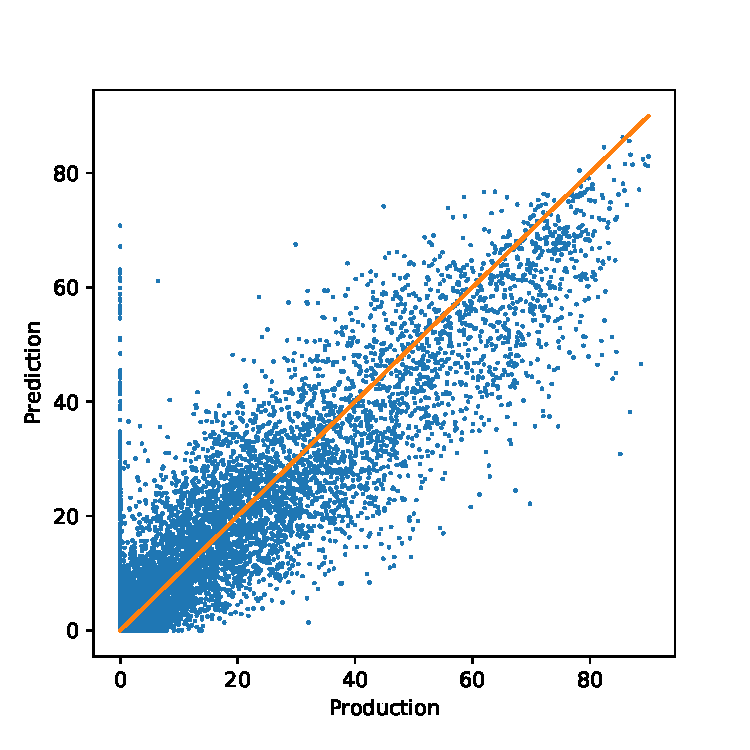
\includegraphics[width=.3 \textwidth, height=.3 \textwidth]{Chapter4/energies/best_ctl_stv.pdf}
    \label{fig:best_ctl_stv}}\quad%
    \subfloat[]{%
    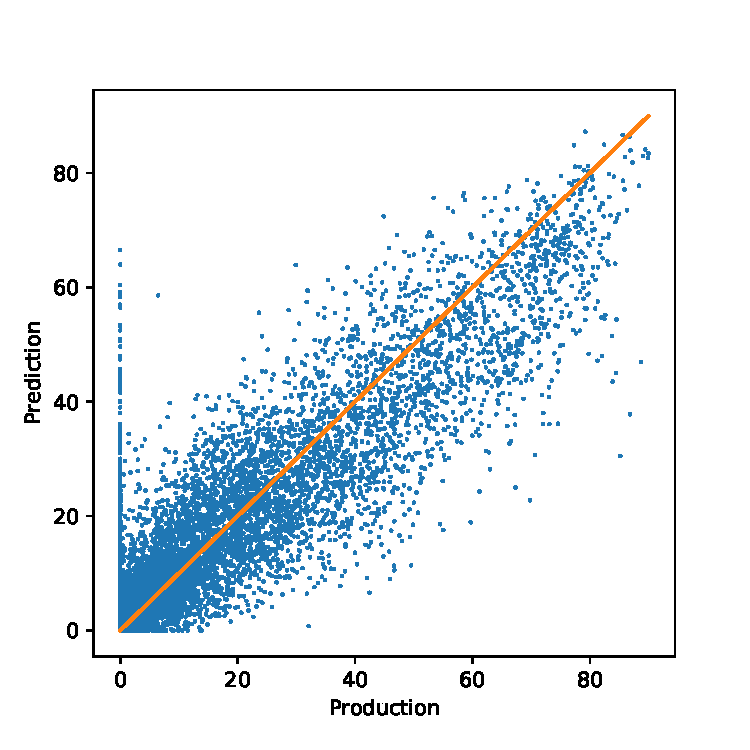
\includegraphics[width=.3 \textwidth, height=.3 \textwidth]{Chapter4/energies/best_itl_stv.pdf}
    \label{fig:best_itl_stv}}\quad%
    \subfloat[]{%
    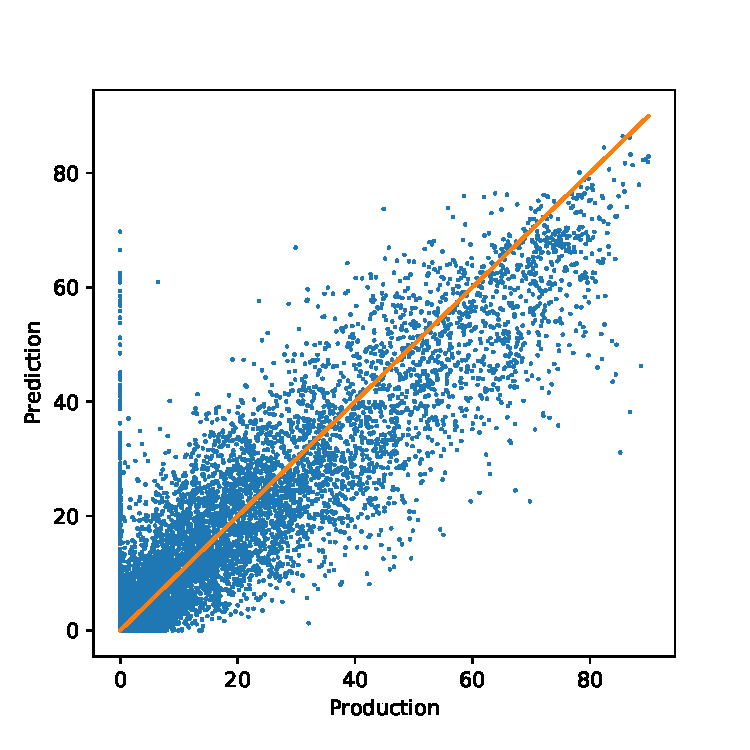
\includegraphics[width=.3 \textwidth, height=.3 \textwidth]{Chapter4/energies/best_mtl_stv.pdf}
    \label{fig:best_mtl_stv}}\\
 \caption{\label{fig:stv_best_plots} Real energy production against prediction made by the best CTL~\protect\subref{fig:best_ctl_stv}, ITL~\protect\subref{fig:best_itl_stv}, and MTL~\protect\subref{fig:best_mtl_stv} models for Sotavento; the perfect prediction line is shown in orange. The~units of the axis are percentages points of the total PV energy~installed.}
 \end{figure}

%
Again, we plot the predictions agains the target values of the CTL model and best ITL,~\fmodt{angle}{itlSVR}, and pure MTL, \fmodt{angle}{mtlSVR} approaches.
The presence of points with zero production is noticeable, but this is relatively frequent in wind energy. It can be caused either by energy curtailments or by maintenance periods of the wind farm.
Also, it is appreciable the frequency of small production values, below \SI{20}{\percent}, which is due to the approximate Weibull distribution of wind speeds, where small speed values have higher frequencies. 
With these considerations, it is difficult to compare the plots and find significant differences in model performance.







% \subsection{Conclusions}

% \paragraph*{old\\}%

% We finally observe that while the wind MAEs in percentage are similar to those in PV, when compared with the energy produced, the~performance of wind models is actually worse.
% In fact, in~Table~\ref{table:comparison} we compare the percentage MAE against the average generated energy as a percentage of installed power.
% As~it can be seen, the~ratio between the percentage MAE and the percentage average energy is about $34.78\%$ for Sotavento, much higher than the $22.50\%$ of Majorca and the $14.92\%$ of~Tenerife.

% \begin{table}[H]
%     \caption{{Comparison}        %Please remove font in the Table
%      of the percentage MAEs with the average energy produced as a percentage of installed~power.}
%     \centering
%     \label{table:comparison}
%     %% \tablesize{} %% You can specify the fontsize here, e.g.,~\tablesize{\footnotesize}. If commented out \small will be used.
%     \begin{tabular}{lccc}
%     \toprule
%  & \fhead{MAE (\%)} & \fhead{Avg. Target (\%)} & \fhead{Ratio} \\
% 	\midrule
% \fdata{majorca} & 6.740 & 29.954 & 22.50 \\
% \fdata{tenerife} & 4.993 & 33.462 & 14.92 \\
% \fdata{sotavento} & 6.186	& 17.784 & 34.78 \\
% \bottomrule
%     \end{tabular}
% \end{table}



\section{Conclusions}\label{sec-conclusions-3}

In this chapter, we have\dots
 % Convex Multi-Task SVM

% Chapter 4

\chapter{Adaptive Graph Laplacian for Multi-Task Learning} % Write in your own chapter title
\label{Chapter5}
\lhead{Chapter \ref{Chapter5}. 
\emph{Adaptive Graph Laplacian Multi-Task Support Vector Machine}} % Write in your own chapter title to set the page header

{\bf \small{

}}

\section{Introduction}
In Chapter~\ref{Chapter3} we divide the \acrfull{mtl} strategies into feature-based, parameter-based and combination-based ones.
The feature-based approaches, which try to find a representation shared by all tasks to obtain leverage in the learning process, rely on the assumption that all tasks can indeed share a common latent representation.
In the case of combination-based, which combines a common part and task-specific parts in the models, a similar belief is held and, although this approach has many good properties, it relies on the assumption that all tasks can share the same common information, which is captured by the common part of the model.
However, this might not be the case in some \acrshort{mtl} scenarios, where there can exist groups of tasks that share some information, but are unrelated to the rest.

%
%Previous work
%
Some parameter-based approaches rely on enforcing low-rank matrices~\citep{AndoZ05,ChenTLY09,PongTJY10}, assuming, thus, that all tasks parameters belong to the same subspace. 
Others try to find the underlying task structure, either by task-relation learning or by clustering the tasks. In the task-relation learning we find strategies using Gaussian Processes and a Bayesian approach such as~\citet{BonillaCW07,ZhangY10}. We also have the \acrfull{gl} approaches, such as the works of~\citet{EvgeniouMP05} or~\citet{argyriou2013learning}, where the tasks are assumed to be nodes of a graph, and the goal is to learn the weights on the edges, which determine the degree of relationship between tasks.
 In these works, iterated algorithms are used to learn both the models parameters and the graph of task-relations.
The clustering approaches are similar, they also use specific regularizers and alternating algorithms to find the clusters.
However, these works using regularization as the mean to enforce the coupling between tasks are limited to linear models.

In general, in the \acrshort{gl} strategies, the idea is based on penalizing the distance between the parameters of different tasks. It is more natural for linear or kernel approaches, where the models for each task $r=1, \ldots, \ntasks$ are defined as
\begin{equation}
    \nonumber
    f_r(x) = w_r \cdot \phi({x}) + b_r
\end{equation}
and $\phi(x)$ is a transformation, which can be the identity $\phi(x)=x$ in linear models, or an implicit transformation to an \acrshort{rkhs} in kernel models.
Here, the models are determined by the parameters $w_r$, so pushing together these parameters enforces the models to be similar. 
The idea is to assume that the relationship between tasks can be modelled using a graph; then, the adjacency matrix $\fm{A}$ of such graph is used to define the regularization
\begin{equation}
    \label{eq:gl_regularization}
    \sum_{r=1}^\ntasks \sum_{s=1}^\ntasks A_{rs} \norm{w_r - w_s}^2 ,
\end{equation}
where $A_{rs}$ are positive scalars that weight the pairwise distances.
Although~\eqref{eq:gl_regularization} is easy to compute for the linear case, it is not that direct in the case of kernel models where, as shown by the Representer Theorem, the optimal parameters $w_r^*$ are elements of an \acrshort{rkhs}.
In this chapter, a framework to use the \acrshort{gl} regularization with kernel models is presented. This is implemented for L1, L2 and LS-SVMs. Moreover, the \acrshort{gl} strategy is combined with the convex \acrshort{mtl} one presented in Chapter~\ref{Chapter4}.
%

Besides, the definition of the weights $A_{rs}$ is not trivial, and it is crucial for the good performance of this strategy. 
First, the values $A_{rs}$ have to be bounded, otherwise its interpretability is lost and, moreover, one term can dominate the sum, so only the models of two tasks would be enforced to be similar.
%
Even with bounded weights, in absence of expert knowledge to select them, it is necessary to find a procedure that finds a set of weights $A_{rs}$ that reflects the real relations between tasks. Because of this, in this chapter, a data-driven procedure to select the weights for a Laplacian regularization is presented.
























%%%%%%%%%%%%%%%%%%%%%%%%%%%%%%%%%%%%%%%%%%%%%%%%%%%%%%%%%%%%%%%%%%%%%%%%%%%%%%%%%%%%%
  %%%%%%%%%%%%%%%%%%%%%%%%%%             SECTION         %%%%%%%%%%%%%%%%%%%%%%%%%%
%%%%%%%%%%%%%%%%%%%%%%%%%%%%%%%%%%%%%%%%%%%%%%%%%%%%%%%%%%%%%%%%%%%%%%%%%%%%%%%%%%%%%

\section{Kernels for Multi-Task Learning}\label{sec:mtl_kernelmethods}

% Most multi-task methods are linear models, which may not be flexible enough to capture certain dependencies.
% Deep Learning is a very popular and cost-effective way of overcoming this problem. The final linear models are substituted by the neural network output and the parameters are learned together using back propagation.
% However, one of the main problems of deep learning is the lack of theoretical results and the non-convexity of the problems.
% Other alternative to extend the \acrshort{mtl} models non-linearly is by using the kernels.

% Most multi-task methods reviewed in Section~\ref{sec:ch3_overview} are based on linear models. This produces the models that are more interpretable and makes it easier to enforce some kind of coupling between tasks so there exists some kind of transfer learning. However, linear models are not powerful enough for most real-world problems, which might have non-linear properties.
% %

% Deep Learning is a very popular and cost-effective way of overcoming this problem. Neural Networks with multiple layers, where each layer may apply a non-linear transformation, are very powerful models that can estimate function using a hierarchical strategy where each new layer builds new features based on the output of the previous layer. 
% This idea is very useful in \acrshort{mtl}, where some features are jointly learned for all the tasks and, in the last layer, final task-specific linear models are build using them.
% %
% Despite its great success, Deep Learning has some inconveniences. One is that to estimate the extensive number of parameters involved in a deep architecture, large quantities of data are needed. This large datasets are not usually of public domain.
% Other problem found in Deep Learning is the lack of mathematical guarantees, at least when compared with other methods of Machine Learning.

% %
% The other alternative to extend \acrshort{mtl} models non-linearly is by using Kernel Methods. Kernel Methods, although they are more computationally challenging, offer some interesting characteristics. In the first place most problems using kernels are formulated as convex problems, which have a single optimum solution. Furthermore, they also offer some well-studied mathematical properties such as consistency of the methods, i.e. the algorithms will approximate this solution as the number of data grows, or rates of convergence, i.e. how fast this solution is approximated.
% Also, Kernel Methods, thanks to this mathematical properties, usually require less data than Deep Learning models to achieve competitive results. 

% % Evgeniou
% \subsection{Regularized \acrshort{mtl}}
% The work of~\cite{EvgeniouP04} presents a \acrshort{svm}-based \acrshort{mtl} problem formulation. 
% The goal is to find a decision function for each task, each being defined by a vector
% $$w_r = w + v_r,$$
% where $w$ is common to all tasks and $v_r$ is task-specific.
% The primal problem of \emph{regularized \acrshort{mtl}} \acrshort{svm}, using the unified formulation, is 
% \begin{equation}
%     \label{eq:regmtlsvm_primal}
%     \begin{aligned}
%         & \argmin_{w, v_r, \xi_i^r}
%         & & C \sum_{r=1}^\ntasks \sum_{i=1}^{\npertask_r} \xi_i^r + \frac{1}{2} \dotp{w}{w} + \sum_{r=1}^\ntasks \frac{\mu}{2} \dotp{v_r}{v_r} \\
%         & \text{s.t.}
%         & & y_{i}^r ( \dotp{w}{x_{i}^r} + \dotp{v_r}{x_{i}^r}) \geq p_i^r - \xi_i^r ,\\
%         & & &\xi_i^r \geq 0, \\
%         & \text{for } & & r=1, \ldots, \ntasks; \; i=1, \ldots, \npertask_r.
%     \end{aligned}
% \end{equation}
% % Leveraging common and specific information
% Note that $\mu$ is a parameter that controls the tradeoff between the relevance of common and specific models. That is, when $\mu$ tends to infinite, the resulting model approaches a common-task standard \acrshort{svm}; when $\mu$ tends to zero, a independent task approach is taken, with one standard \acrshort{svm} problem for each task.
% This is also reflected in the corresponding dual problem
% \begin{equation}\label{eq:regmtlsvm_dual}
%     \begin{aligned}
%         & \argmin_{\alpha_i} 
%         & & \frac{1}{2} \sum_{r, s=1}^\ntasks \sum_{i, j=1}^{\npertask_r} y_i^r y_j^s \alpha_i^r \alpha_j^s \dotp{x_i^r}{x_j^s} + \frac{1}{2 \mu} \sum_{r, s=1}^\ntasks  \sum_{i, j=1}^{\npertask_r} y_i^r y_j^s \alpha_i^r \alpha_j^s \delta_{rs} \dotp{x_i^r}{x_j^s} \\
%         & & & \qquad - \sum_{r=1}^\ntasks \sum_{i=1}^{\npertask_r} p_i^r \alpha_i^r \\
%         & \text{s.t.}
%         & & 0 \leq \alpha_i^r \leq C \\
%         & \text{for } & & r=1, \ldots, \ntasks; \; i=1, \ldots, \npertask_r.
%         \end{aligned}
% \end{equation}
% In this dual form, as $\mu$ grows, the task-specific part goes to zero, and the most important term is the first one, corresponding to the common part. The opposite effect is obtained when $\mu$ shrinks.
% % Common + specific model which is equivalent to penalizing individual norm and variance
% Moreover, in~\cite{EvgeniouP04} it is shown that solving~\eqref{eq:regmtlsvm_primal} is equivalent to solving the problem
% \begin{equation}
%     \nonumber
%     \begin{aligned}
%         & \argmin_{ww_r, \xi_i^r}
%         & & C \sum_{r=1}^\ntasks \sum_{i=1}^{\npertask_r} \xi_i^r +  \frac{1}{2} \sum_{r=1}^\ntasks \norm{w_r}^2 + \frac{\mu}{2} \sum_{r=1}^\ntasks  \norm{w_r - \sum_{s=1}^\ntasks w_s}^2 \\
%         & \text{s.t.}
%         & & y_{i}^r ( \dotp{w_r}{x_{i}^r}) \geq p_i^r - \xi_i^r ,\\
%         & & &\xi_i^r \geq 0, \\
%         & \text{for } & & r=1, \ldots, \ntasks; \; i=1, \ldots, \npertask_r.
%     \end{aligned}
% \end{equation}
% Now, only the $w_r$ variables are included, and it is clearer that $\mu$ penalizes the variance of the $w_r$ vectors, so all models $w_r$ will tend to a common model as $\mu$ grows.


% Kernels are functions that are used as a measure of similarity between data points, and have a notable relevance in \acrshort{ml} due to the success of kernel methods, such as the \acrshort{gp} or \acrshort{svm}. 
% %
% % Moreover, when using kernel methods, the parametric point of view for estimating a function of the primal formulation is changed for a non-parametric one in the dual problem, where the complexity of the model increase with the number of examples.
% However, as we have observed in the previous section, designing \acrshort{mtl} is not a trivial task, and the proposals are fewer than those of linear models or \acrshort{nns}. 
% Although the combination-based MTLSVM has a strong motivation in the \acrshort{lupi} paradigm, it assumes a common model for all tasks, which may not be always useful. Other approaches consider the pairwise task relations, so a more fine-grained inter-task coupling can be imposed.
% In this section, we give some definitions and propose a formulation to extend some useful results, heading in this direction, for linear models, namely those of~\cite{EvgeniouMP05}, to kernelized ones.

In \acrshort{mtl} different functions have to be estimated and the relation between those task-specific functions is desirable to be captured. Using kernels for these goals imposes some new challenges, that can be tackled from different perspectives. 
% Learning Multiple Tasks with Kernel Methods
One of them is interpreting the \acrshort{mtl} paradigm so that it can be seen as learning a vector-valued function, thus using a vector-valued \acrfull{rkhs}. We define this and some related contents, and also describe an extension of the Representer Theorem for vector-valued \acrshort{rkhs} problems.
%
Also, here we propose a reformulation where a tensor product of scalar \acrshort{rkhss} is used instead of the vector-valued ones, which leads to some more general results, including another extension of the Representer Theorem.
%
Finally, we take these definitions to show how to use them to solve \acrshort{mtl} problems and also give some examples of commonly used \acrshort{mt} kernels.


\subsection{Vector-Valued Reproducing Kernel Hilbert Spaces}%Single-Task Learning with \acrshort{mtl} Kernels}
To give different definitions of vector-valued kernels, we will follow the work of~\citet{MicchelliP05}.
Consider $\Yspace$ a Hilbert space with inner product $\ydotp{.}{.}$, and $\mathcal{L}(\Yspace)$ the space of linear operators from $\Yspace$ to $\Yspace$; then we can study the Hilbert spaces $\hilbertspace$ of functions
\begin{equation*}
    \begin{aligned}
        f: &&\Xspace&& &\to& &&&\Yspace&& \\
             && x&&      &\to& &&& f(x) &&
    \end{aligned}
\end{equation*}
with inner product $\dotp{\cdot}{\cdot}$.
The kernels in such spaces are operator-valued functions $K: \Xspace \times \Xspace \to \mathcal{L}(\Yspace)$.
We look at these spaces from three different and equivalent perspectives: continuous evaluation functionals, positive-definite kernels and feature maps.

%\paragraph*{Continuous evaluation functionals.}
The first approach considered is that of continuous evaluation functionals.
% Given a Hilbert space with continuous evaluation functionals, which are defined later, we can find the reproducing kernel operator.
Consider the vector-valued Hilbert space $\mathcal{H}$ with inner product $\dotp{\cdot}{\cdot}$ of functions defined in $\Xspace$ and values in $\Yspace$, and the functionals 
%$L_{x, y} f = \ydotp{y}{f(x)}$,
\begin{equation*}
    \begin{aligned}
        L_{x, y}:&&\hilbertspace& &\to& &&\Yspace&& &\to& &&\reals& & \\
        &&f& &\to& &&f(x)&& &\to& &&\ydotp{y}{f(x)}& &
    \end{aligned}.
\end{equation*}
If these functionals are continuous, we can apply Riesz representation theorem~\citep{riesz2012functional}. That is, for every $x \in \Xspace, y \in \Yspace$ we can find an unique $g_{x, y} \in \hilbertspace$ such that for all $f \in \hilbertspace$,
\begin{equation}\label{eq:vector_riesz}
    L_{x, y} f = \ydotp{y}{f(x)} = \dotp{g_{x,y}}{f}_{\hilbertspace} .
\end{equation}
We can now give the definition of vector-valued Hilbert space from the point of view of continuous functionals as in~\citet[Definition 2.1]{MicchelliP05}.
\begin{definition}[vector-valued RKHS]
    We say that $\hilbertspace$ is a vector-valued RKHS when for any $x \in \Xspace$ and $y \in \Yspace$, the functional $L_{x, y} f = \ydotp{y}{f(x)}$ is continuous.
\end{definition}
Note that this is a definition similar to the scalar case but we use the inner product of $\Yspace$ to construct the scalar-valued functionals $L_{x, y}$. The price we pay is that it is necessary to express the Riesz representation as dependent of the elements $y \in \Yspace$. To get rid of this dependence, for every $x \in \Xspace$ we can define the linear operator
\begin{equation}
    \label{eq:vector_riesz}
    \begin{aligned}
        g_x: &&\Yspace&& &\to& &&&\hilbertspace&& \\
             && y&&      &\to& &&g_x y &= g_{x, y} &&
    \end{aligned}.
\end{equation}
This operator is well defined because $g_{x, y}$ is unique for every $x \in \Xspace, y \in \Yspace$ and its linearity is easy to check from the linearity of the inner product $\ydotp{.}{.}$.
%
Using these results, we can now define the operator
\begin{equation}\label{eq:vector_kernel}
    \begin{aligned}
        K(x, \hat{x}) : &&\Yspace&& &\to& &&&\Yspace&& \\
                        && y &&     &\to& &&K(x, \hat{x}) y &= (g_{\hat{x}} y) (x)&&
    \end{aligned}    
\end{equation}
for every $x, \hat{x} \in \Xspace$. 
%Observe that $K(x, \hat{x})$ is linear since $\forall x,\;  g_x$ is linear, i.e. $g_x(\lambda_1 y_1 + \lambda_2 y_2) = \lambda_1 g_x(y_1) + \lambda_2 g_x(y_2)$.
It is possible then to prove that $K(x, \hat{x})$ is a reproducing kernel in $\mathcal{H}$ as seen in~\citet[Propositon 2.1]{MicchelliP05}.

\begin{proposition}
    If $K(x, \tilde{x})$ is defined for every $x, \hat{x} \in \Xspace$ as in ~\eqref{eq:vector_kernel} and $g_x$ is defined as in ~\eqref{eq:vector_riesz}, then
    \begin{equation}
        \nonumber
        K: \Xspace \times \Xspace \to \mathcal{L}(\Yspace)
    \end{equation}
    is a kernel that for every $x, \hat{x} \in \Xspace$ satisfies:
    \begin{enumerate}
        \item For every $y, \hat{y} \in \Yspace$, we have 
        \begin{equation}
            \nonumber
            \ydotp{y}{K(x, \tilde{x}) \hat{y}} = \dotp{g_x \hat{y}}{g_{\hat{x}} y} .
        \end{equation}
        \item $K(x, \tilde{x}) = \adj{K(\tilde{x}, x)}$ and $K(x, x)$ is positive definite for every $x \in \Xspace$.
        \item Given $n \in \naturals$, for any  $x_1, \ldots, x_n \in \Xspace,  y_1, \ldots, y_n \in \Yspace$,
        \begin{equation}
            \nonumber
            \sum_{i, j =1}^n \ydotp{y_i}{K(x_i, x_j) y_j} \geq 0.
        \end{equation}
        \item $\norm{g_x} = \norm{K(x, x)}^{\frac{1}{2}}$.
        \item $\norm{K(x, t)} \leq \norm{K(x, x)}^{\frac{1}{2}} \norm{K(t, t)}^{\frac{1}{2}}$.
        \item For every $f \in \hypspace$ and $x \in \Xspace$, we have that
        $$ \norm{f(x)} \leq \norm{f} \norm{K(x, x)}^{\frac{1}{2}} .$$
    \end{enumerate}
\end{proposition}

% To do that, first we have to define a vector-valued kernel and the corresponding reproducing property.
% \begin{definition}[operator-valued Kernel]
%     Given a non-empty set $\Xspace$, if $\Yspace$ is a finite-dimensional Hilbert space
%     % , and $\hilbertspace$ is a Hilbert space of $\Yspace$-valued functions with domain in $\Xspace$
%      an operator-valued kernel is a function
%     \begin{equation}
%         \nonumber
%         K: \Xspace \times \Xspace \to \mathcal{L}(\Yspace)
%     \end{equation}
%     which is symmetric and positive definite.
% \end{definition}
% For the clarity of the text an operator-valued $K$ will be referred just as a kernel unless an explicit distinction is needed.
% \begin{definition}[Reproducing Property of operator-valued operators]
%     If $\Yspace$ is a finite-dimensional Hilbert space, and $\hilbertspace$ is a Hilbert space of $\Yspace$-valued functions with domain in $\Xspace$, a function
%     \begin{equation}
%         \nonumber
%         K: \Xspace \times \Xspace \to \mathcal{L}(\Yspace)
%     \end{equation}
%     has the reproducing property if $\forall x \in \Xspace, y \in \Yspace, \forall f \in \hilbertspace,$ 
%     $$ \ydotp{y}{f(x)} = \dotp{K(\cdot, x) y}{f}_\hilbertspace.$$ 
% \end{definition}
% A kernel with the reproducing property is also called a reproducing kernel. The next proposition shows how we can build a reproducing kernel for a space $\hilbertspace$ in which the evaluation functionals are continuous.
% \begin{proposition}
%     If for every $x, \hat{x} \in \Xspace$, the function $K(x, \hat{x})$ is defined as in Equation~\eqref{eq:vector_kernel}, then the function
%     \begin{equation}
%         \nonumber
%         K: \Xspace \times \Xspace \to \mathcal{L}(\Yspace)
%     \end{equation}
%     is a reproducing kernel.
% \end{proposition}
% \begin{proof}
%     To prove that $K$ is a reproducing kernel we need to check: 
%     \begin{enumerate}
%         \item\label{item:vvkernel_bounded} $K(x, \hat{x})$ is bounded for every $x, \hat{x} \in \Xspace$ so $K$ is well defined.
%         \item\label{item:vvkernel_symmetric} $K$ is symmetric: $\adj{K(x, \hat{x})} = K(\hat{x}, x)$, where $\adj{A} \in \mathcal{L}(\Yspace)$ is the adjoint of $A \in \mathcal{L}(\Yspace)$.
%         \item\label{item:vvkernel_positive}  $K$ is positive definite: given $n \in \naturals$, for any  $x_1, \ldots, x_n \in \Xspace,  y_1, \ldots, y_n \in \Yspace$,
%         \begin{equation}
%             \nonumber
%             \sum_{i, j =1}^n \ydotp{y_i}{K(x_i, x_j) y_j} \geq 0.
%         \end{equation}
%         \item\label{item:vvkernel_repr} It has the reproducing property: $\forall x \in \Xspace, y \in \Yspace, \forall f \in \hilbertspace,$ $ \ydotp{y}{f(x)} = \dotp{K(\cdot, x) y}{f}.$
%     \end{enumerate}
%     To prove~\ref{item:vvkernel_bounded} and~\ref{item:vvkernel_symmetric}, observe that by
%     applying~\eqref{eq:vector_riesz} to $f = g_{\hat{x}}\hat{y}$, for every $x \in \Xspace, y \in \Yspace$ there exists an unique $g_{x, y} = g_{x}y$ such that
%     \begin{equation}
%         \ydotp{y}{(g_{\hat{x}} \hat{y}) (x)} = \dotp{g_{x}y}{g_{\hat{x}}\hat{y}} ,
%     \end{equation}
%     and combining this result with~\eqref{eq:vector_kernel} we get
%     \begin{equation}
%         \nonumber
%         \ydotp{y}{K(x, \hat{x}) \hat{y}} = \ydotp{y}{(g_{\hat{x}} \hat{y})(x) }= \dotp{g_{x}y}{g_{\hat{x}}\hat{y}}.
%     \end{equation}
%     Also, using the definitions,
%     \begin{equation}
%         \nonumber
%         \ydotp{K(\hat{x}, x) y}{ \hat{y}} = \ydotp{(g_{x} y)(\hat{x})}{\hat{y}} = \ydotp{\hat{y}}{(g_{x} y)(\hat{x})} = \dotp{g_{\hat{x}} \hat{y}}{g_x y}.
%     \end{equation}
%     Since both operators $K(x, \hat{x}), K(\hat{x}, x)$ are bilinear, by the Uniform Boundness Principle~\citep{Akhiezer1961TheoryOL}, $K(x, \hat{x}), K(\hat{x}, x)$ are bounded (hence continuous) and $K(x, \hat{x})^* = K(\hat{x}, x)$.
%     \\
%     To prove~\ref{item:vvkernel_positive} we write
%     \begin{equation}
%         \nonumber
%         \sum_{i, j =1}^n \ydotp{y_i}{K(x_i, x_j) y_j} = \sum_{i, j =1}^n \dotp{g_{x_i} y_i}{g_{x_j} y_j}  = \norm{\sum_{i=1}^n g_{x_i} y_i}^2 \geq 0 .
%     \end{equation}
%     Finally, to prove~\ref{item:vvkernel_repr} we use that 
%     $\forall x \in \Xspace, y \in \Yspace, \forall f \in \hilbertspace, \exists g_{x, y} \in \hilbertspace$ such that 
%     $$ \ydotp{y}{f(x)} = \dotp{g_{x, y}}{f} = \dotp{g_{x} y}{f} =\dotp{K(\cdot, x) y}{f}.$$
% \end{proof}

%\paragraph*{Positive semi-definite kernels.}
The second approach of~\citet{MicchelliP05} to define vector-valued kernels changes the point of view. Given a kernel $K$, the Hilbert space from which $K$ is the reproducing kernel is built.
To do this, we use~\citet[Theorem 2.1]{MicchelliP05}, which extends the Moore-Aronszanj Theorem:
\begin{theorem}\label{th:moore-arons_vector}
    If $K: \Xspace \times \Xspace \to \mathcal{L}(\Yspace)$ is a kernel, then there exists a unique (up to an isometry) RKHS which admits $K$ as its reproducing kernel. 
\end{theorem}
The proof is similar to that of the Moore-Aronszanj Theorem, considering the space of the completion of the span of $\left\lbrace K_x = K(\cdot, x) , x \in \Xspace \right\rbrace$.

%\paragraph*{Feature map.}
The last approach is based on feature maps, which provide a very simple way of generating kernels.
\begin{lemma}
    Given some Hilbert space $\mathcal{W}$, any continuous feature map $\Phi: \Xspace \to \mathcal{L}(\mathcal{W}, \mathcal{Y})$ defines a kernel as
\begin{equation}
    \label{eq:kernel_featmap}
    K(x, \hat{x}) = \Phi(x) \circ \adj{\Phi(\hat{x})}: \Yspace \to \Yspace .
\end{equation}
\end{lemma}
\begin{proof} We need to prove that it is bounded, symmetric and positive definite:
    \begin{enumerate}
        \item Since $\Phi(x)$ is continuous, its adjoint $\adj{\Phi(x)}$ is continuous and the composition $\Phi(x) \circ \adj{\Phi(\hat{x})}$ is also continuous.
        \item It is symmetric since  $\adj{(\Phi(x) \circ \adj{\Phi(\hat{x})})} = (\adj{(\adj{\Phi(x)})} \circ \adj{\Phi(\hat{x})}) = (\Phi(x) \circ \adj{\Phi(\hat{x})}) $.
        \item It is semipositive definite since, given any $x_1, \ldots, x_n \in \Xspace,  y_1, \ldots, y_n \in \Yspace$
        \begin{equation}
            \nonumber
            \begin{aligned}
                \sum_{i, j =1}^n \ydotp{y_i}{K(x_i, x_j) y_j} &= \sum_{i, j =1}^n \ydotp{y_i}{ \Phi(x_i) \circ \adj{\Phi(x_j)} y_j} \\
                & = \sum_{i, j =1}^n \ydotp{\adj{\Phi(x_i)} y_i}{ \adj{\Phi(x_j)} y_j} = \norm{\sum_{i=1}^n \adj{\Phi(x_i)} y_i}^2 \geq 0 .
            \end{aligned}
        \end{equation}
    \end{enumerate}
\end{proof}
% Since $K$ as defined in~\eqref{eq:kernel_featmap} is a kernel, according to Theorem~\ref{th:moore-arons_vector} we can find its corresponding vector-valued Hilbert space $\hilbertspace$.

%\subsubsection*{Representer Theorem for Operator-Valued Kernels}
These definitions related to vector-valued \acrshort{rkhss} are useful to get a better understanding of how to apply operator-valued kernels for learning multi-target or multi-task functions. Concretely, we would like to develop some result similar to representer theorem~\cite{ScholkopfHS01}, which is a crucial result in optimization and \acrshort{ml}. Given a regularized empirical risk, under some assumptions, the theorem gives a precise description of the minimizer $f^*$ as a finite linear combination of functions $K(\cdot, x_i)$ where $x_i$ are part of the empirical sample.
This result is extended in~\citet[Theorem 4.2]{MicchelliP05} for operator-valued kernels through the next theorem.
\begin{theorem}
    Let $\mathcal{Y}$ be a Hilbert space and let $\mathcal{H}$ be the Hilbert space of $\mathcal{Y}$-valued functions with an operator-valued reproducing kernel $K$. Let $V: \Yspace^n \times \reals_+ \to \reals$ be a function strictly increasing in its second variable and consider the problem of minimizing the functional    
    \begin{equation}\label{eq:representer_functional}
        \begin{aligned}
            E(f) = V((f(x_1), \ldots, f(x_n)), \norm{f}^2)
        \end{aligned}
    \end{equation}
    in $\hilbertspace$.
    If
    % for every $(f_1, \ldots, f_n) \in \Yspace^n$ the function $h: \reals_+ \to \reals_+$ defined as $h(t) = V((f_1, \ldots, f_n)), t)$ is strictly increasing and
    $f_0$ minimizes $E$, then $f_0 = \sum_{j=1}^n K(\cdot, x_j) c_j$ where $c_j \in \mathcal{Y}$. In addition, if $V$ is strictly convex, the minimizer is unique. 
\end{theorem}
% The proof can be found in~\citet{MicchelliP05}.

%\subsubsection*{Bijection between Scalar and Vector-Valued Kernels}
The scalar-valued kernels are well known and studied but this is not the case for operator-valued kernels. However, as shown in~\cite{Hein04kernels,BaldassarreRBV12}, we can find a bijection between operator-valued kernels and scalar-valued ones.
\begin{lemma}\label{lemma:kernel_bijection}
    Let $\mathcal{Y}$ be a finite-dimensional Hilbert space and
    $K: \Xspace \times \Xspace \to \mathcal{L}(\mathcal{Y})$
    be an operator-valued kernel. Consider also the scalar-valued kernel
    $L: (\Xspace, \mathcal{Y}) \times (\Xspace, \mathcal{Y}) \to \reals$
    such that $L((x, z), (\hat{x}, \hat{z})) = \ydotp{z}{K(x, \hat{x}) \hat{z}}$. Then the map $K \to L$ is a bijection.
\end{lemma}
Moreover, if we focus on finite dimensional Hilbert spaces, that is, isomorphic to $\reals^d$, given an operator-valued kernel $K$, the corresponding scalar-valued kernel $L$ is defined using the normal basis as
$$ L((x, e_r), (\hat{x}, e_s)) = \ydotp{e_r}{K(x, \hat{x}) e_s} = K(x, \hat{x})_{rs} ; \; r,s=1, \ldots, \dimx.$$
That is, each pair $(x, \hat{x})$ defines a matrix which contains the information of how the different outputs, or tasks, are related.
 
% \begin{figure}[t]
%     \centering
% \begin{tikzpicture}[node distance=1cm, auto,]
%     %nodes
%     \node[punkt] (market) {Market (b)};
%     % We make a dummy figure to make everything look nice.
%     \node[above=of market] (dummy) {};
%     \node[right=of dummy] (t) {Ultimate borrower}
%       edge[pil,bend left=45] (market.east) % edges are used to connect two nodes
%     \node[left=of dummy] (g) {Ultimate lender}
%       edge[pil, bend right=45] (market.west)
%       %edge[pil,<->, bend left=45] node[auto] {Direct (a)} (t);
% \end{tikzpicture}
% \caption{Bijections between kernel functions.}
% \end{figure}

% \begin{figure}[t]
%     \centering
% \begin{tikzpicture}[node distance=1cm, auto,]
%     %nodes
%     \node[] (w) {};
% \end{tikzpicture}
% \caption{Bijections between kernel functions.}
% \end{figure}


\subsection{Tensor Product of Reproducing Kernel Hilbert Spaces}
Given two finite-dimensional vector spaces $V$ and $W$ over a field $F$, with dimensions $n$ and $m$, the tensor product of these spaces, $V \otimes W$, is associated with the bilinear map
\begin{equation}
    \nonumber
    \begin{aligned}
        &V \times W &\to V &\otimes W & \\
    &(v, w)  &\to v &\otimes w &
    \end{aligned},
\end{equation}
such that
\begin{equation}
    \nonumber
    \begin{bmatrix}
        v_1 \\
        \vdots \\
        v_n
    \end{bmatrix}
    \otimes 
    \begin{bmatrix}
        w_1 \\
        \vdots \\
        w_n
    \end{bmatrix}
    =
    \begin{bmatrix}
        v_1 w_1 \\
        \vdots \\
        v_1 w_n \\
        \vdots \\
        v_m w_1 \\
        \vdots \\
        v_m w_n \\
    \end{bmatrix} .
\end{equation}
This tensor product can be constructed from the basis of the vector spaces. Consider $B_V$ and $B_W$ the basis of $V$ and $W$, respectively, then the tensor product $V \otimes W$ is a vector space which has as basis the set $\set{v \otimes w, \; v \in B_V, \; w \in B_W}$.
%
Since this definition seems recursive, we can also recur to the interpretation of the tensor product as a quotient space.
Let $L$ be the vector space that has the Cartesian product $V \times W$ as its basis. Let $R$ be the linear subspace of $L$ that is the span of the elements of one of the following forms:
\begin{align*}
    (v_1 + v_2, w) - (v_1, w) - (v_2, w), \\
    (v, w_1 + w_2) - (v, w_1) - (v, w_2), \\
    (sv, w) - s(v, w), \\
    (v, sw) - s(v, w), 
\end{align*}
where $v, v_1, v_2 \in V$, $w, w_1, w_2 \in W$ and $s \in F$. Then, we can define the tensor product space as the quotient space $L/R$. Observe that these are just the relations to ensure that the tensor product is a bilinear application.
More concretely, we can name this definition as the algebraic tensor product of vector spaces and denote it as $V \otimes_{\text{alg}} W$, which is equivalent to $V \otimes W$ in the finite dimensional case.
If $\hilbertspace_1$ and $\hilbertspace_2$ are finite-dimensional Hilbert spaces, then the tensor product space $\hilbertspace_1 \otimes \hilbertspace_2$ is a Hilbert space with inner product
\begin{equation}
    \label{eq:innerprod_tensor}
    \begin{aligned}
        \dotp{}{}:\;  &(\rkhs_1 \otimes \rkhs_2) &\times& &(\rkhs_1 \otimes \rkhs_2) &\to &\reals &&  \\
    &(f_1 \otimes f_2) && &(\hat{f}_1 \otimes \hat{f}_2) &\to &\dotp{f_1}{\hat{f}_1} & \dotp{f_2}{\hat{f}_2} &.
    \end{aligned}
\end{equation}
%
Extending this definition to the infinite-dimensional case is not trivial, and we follow roughly the work of~\citet{Kadison1983}. 
%Let $X_1, X_2$ be finite-dimensional vector spaces.
Consider the \acrshort{rkhss} $\hilbertspace_1$ of functions  $f: \Xspace_1 \to \reals$ and  $\hilbertspace_2$ of functions $g: \Xspace_2 \to \reals$, with the quotient space definition we can define the tensor product space $H_1 \otimes_{\text{alg}} H_2$ of functions
\begin{equation}\nonumber
    \begin{aligned}
        f \otimes_{\text{alg}} g:\;  &\Xspace_1 &\times & &\Xspace_2 &\to &&\reals \\
            &(x_1 & , & &x_2) &\to  &f(x_1) &  g(x_2) ,
    \end{aligned}
\end{equation}
which is a pre-Hilbert space with the inner product defined in~\eqref{eq:innerprod_tensor}.
We can complete this space, i.e. include the limits of the Cauchy series, to get the corresponding Hilbert space~\citep{Kadison1983}, that we will denote as $\rkhs_1 \otimes \rkhs_2$.

% Also, consider $\hilbertspace_1 \otimes \hilbertspace_2$ as the space of the tensor product of two scalar-valued RKHS' $\hilbertspace_1$ and $\hilbertspace_2$ with reproducing kernels $K_1, K_2$, where the functions $f \in \hilbertspace_i$ are defined as $f: \Xspace_i \to \Yspace_i$ for $i=1, 2$. This tensor space is also a Hilbert space endowed with the inner product:
% \begin{equation}
%     \label{eq:innerprod_tensor}
%     \begin{aligned}
%         \dotp{}{}: &(\rkhs_1 \otimes \rkhs_2) &\times& &(\rkhs_1 \otimes \rkhs_2) &\to &\reals &&  \\
%     &(f_1 \otimes f_2) && &(\hat{f}_1 \otimes \hat{f}_2) &\to &\dotp{f_1}{\hat{f}_1} & \dotp{f_2}{\hat{f}_2} &.
%     \end{aligned}
% \end{equation}
% It is easy to check that this inner product is symmetric because the inner products of both $\hilbertspace_1$ and $\hilbertspace_2$ are symmetric. It is linear because the inner products of both $\hilbertspace_1$ and $\hilbertspace_2$ are linear and the tensor product is linear. Finally, it is positive definite since 
% $  \dotp{f_1}{f_1}  \dotp{f_2}{f_2} \geq 0$ and
% $\dotp{f_1}{f_1}  \dotp{f_2}{f_2} = 0 \implies \dotp{f_i}{f_i} = 0$ for $i=1$ or $i=2$; taking $i=1$ without loss of generality, then $f_1 = 0$, so $f_1 \otimes f_2 = 0 \in \rkhs_1 \otimes \rkhs_2$. 
To apply the Riesz Theorem in this Hilbert space it is necessary to check whether the evaluation functionals are continuous or, equivalently, bounded.
%
\begin{proposition}[\acrshort{rkhs} as tensor product of \acrshort{rkhs}']\label{prop:bounded_tensorfun}
    Let $\rkhs_1$ and $\rkhs_2$ be \acrshort{rkhss} ; then
    the space $\hilbertspace = \hilbertspace_1 \otimes \hilbertspace_2$ , with evaluation functionals $L_{(x_1, x_2)} $ defined as 
    $$L_{(x_1, x_2)} (f_1 \otimes f_2) =L_{x_1}(f_1) \otimes L_{x_2}(f_2) = f_1(x_1) \otimes f_2(x_2)$$
    for $x_1 \otimes x_2 \in \Xspace_1 \otimes \Xspace_2$,
     is an \acrshort{rkhs} with the inner product defined in~\eqref{eq:innerprod_tensor}. 
\end{proposition}
\begin{proof}
    It is necessary to ensure that the operators $L_{(x_1, x_2)}$ are bounded. Given any $f_1 \otimes f_2 \in \hilbertspace_1 \otimes \hilbertspace_2$, 
    $$ \norm{L_{(x_1, x_2)} (f_1 \otimes f_2)} = \dotp{f_1(x_1)}{f_1(x_1)} \dotp{f_2(x_2)}{f_2(x_2)} \leq \norm{f_1(x_1)}^2  \norm{f_2(x_2)}^2 .$$
    Then, since $\hilbertspace_1$ and $\hilbertspace_2$ are bounded, the product 
$ \norm{f_1(x_1)}  \norm{f_2(x_2)} $
is also bounded.
\end{proof}

%
We also need to define the kernel function for this tensor product space.
\begin{proposition}
    Let $\rkhs_1$ and $\rkhs_2$ be \acrshort{rkhss} whose reproducing kernel are $K_1$ and $K_2$, respectively;
    then the function
    \begin{equation}
        \nonumber
        \begin{aligned}
            K_1 \otimes K_2: &(\Xspace_1 \times \Xspace_2) &\times &&(\Xspace_1 \times \Xspace_2) &\to && \reals & \\
        &(x_1 , x_2) & &&(\hat{x}_1 , \hat{x}_2) &\to & K_1(x_1, \hat{x}_1)  & K_2(x_2, \hat{x}_2) & ,
        \end{aligned}
    \end{equation}
    is a reproducing kernel for the Hilbert space $\hilbertspace_1 \otimes \hilbertspace_2$.
\end{proposition} 
\begin{proof}
    First, observe that $(K_1 \otimes K_2)^{(x_1 , x_2)} =  K_1^{x_1} \otimes K_2^{x_2}  \in \rkhs_1 \otimes \rkhs_2$,
    where 
    \begin{equation}\nonumber
        \dotp{K_1^{x}}{f} = f(x) , \; \forall f \in \rkhs_1 \text{ such that } K_1(x, \hat{x}) = \dotp{K_1^{x}}{K_1^{\hat{x}}} 
    \end{equation}
    and 
    \begin{equation}\nonumber
        \dotp{K_2^{x}}{g} = g(x) , \; \forall g \in \rkhs_2 \text{ such that } K_2(x, \hat{x}) = \dotp{K_2^{x}}{K_2^{\hat{x}}} ,
    \end{equation}
    satisfies that for every $f \otimes g \in \rkhs_1 \otimes \rkhs_2$, 
    \begin{equation}\nonumber
        \dotp{(K_1 \otimes K_2)^{(x_1 , x_2)}}{f \otimes g} = f(x_1) g(x_2) .
    \end{equation}
    Since the evaluation functionals are bounded as shown in Proposition~\ref{prop:bounded_tensorfun}, by the Riesz theorem, for every $(x_1 , x_2) \in \Xspace_1 \otimes \Xspace_2$ there exists a single element $K_{(x_1 , x_2)} \in \rkhs_1 \otimes \rkhs_2$ such that
    \begin{equation}
        \nonumber
        \dotp{K_{(x_1 , x_2)}}{f \otimes g}\;  \forall f \otimes g \in \rkhs_1 \otimes \rkhs_2 ,
    \end{equation}
    thus, this element must be $K_{(x_1 , x_2)} = (K_1 \otimes K_2)^{(x_1 , x_2)}$.
    %

    Then, we can define 
    \begin{align*}
        (K_1 \otimes K_2)((x_1 , x_2), (\hat{x}_1 , \hat{x}_2)) &= \dotp{(K_1 \otimes K_2)^{(x_1 , x_2)}}{(K_1 \otimes K_2)^{(\hat{x}_1 , \hat{x}_2)}} \\
        & = \dotp{K_1^{x_1} \otimes K_2^{x_2}}{K_1^{\hat{x}_1} \otimes K_2^{\hat{x}_2}} \\
        &= \dotp{K_1^{x_1}}{K_1^{\hat{x_1}}} \dotp{K_2^{x_2}}{K_2^{\hat{x_2}}} \\
        &= K_1(x_1, \hat{x}_1) K_2(x_2, \hat{x}_2) .
    \end{align*}
    

    We observe that $K_1 \otimes K_2$ is symmetric and positive-definite because both $K_1$ and $K_2$ are symmetric and positive definite, %The proof is very similar to the symmetry and positive definiteness proof of the inner product~\eqref{eq:innerprod_tensor}.
    and, by construction, it has the reproducing property.
\end{proof}

%\subsubsection*{Separable Kernels}
To understand the connection between tensor product RKHS's and vector-valued RKHS's we study a special case of operator-valued kernels.
A standard assumption is that the relation among the different outputs is independent of the pair $(x, \hat{x})$, that is, the kernel is separable~\citep{AlvarezRL12, KadriDPCRA16}.
\begin{definition}[Separable Kernel]
    An operator-valued kernel $K(x, \hat{x}): \Yspace \to \Yspace$ is called separable if
    $$ K(x, \hat{x})  = k(x, \hat{x}) M$$
    here $k(\cdot, \cdot)$ is a scalar-valued kernel and $M$ is some fixed operator $M \in \mathcal{L}(\mathcal{Y})$.
\end{definition}
That is, the operator $K(x, \hat{x})$ decouples in two parts: the similarity between $x$ and $\hat{x}$ measured by $k(\cdot,\cdot)$ and the interaction between the different outputs expressed by $M$. 
%In those cases it is easier to express the operator-valued kernel as the tensor product of two spaces. 
%The following lemma shows how we can express such tensor product kernel.
%
% Consider the tensor product space $\Xspace \otimes \Tspace$, where $\Tspace$ is the space of tasks. We assume that $\Tspace$ has finite dimension, therefore it is isomorphic to $\reals^k$. We consider $\hilbertspace$ as the Hilbert space of functions $f: \Xspace \to \reals$ with reproducing kernel $K_\Xspace$, and $\Tspace = (\reals^k)^*$ as the space of linear functions $g: \reals^k \to \reals$, which is isomorphic to $\reals^k$. In $\reals^k$ we consider a general inner product induced by the positive definite matrix $A$.
% Then $(\reals^k)^*$, by the Riesz Representation Theorem, $ \forall x \in \reals^k, \exists u_x \in (\reals^k)^*$ such that $\forall w \in (\reals^k)^*$ 
% $$ \dotp{w}{u_x}_A = w x, $$
% that is, $u_x = A^{-1}x$.
% Then, the kernel is defined as
% $K_{\Tspace}(x, y) = \dotp{u_x}{u_y}_A = x^\intercal A^{-1} y$.
% Now we can define the following tensor product of two scalar-valued kernels:   
% \begin{equation}
%     \nonumber
%     \begin{aligned}
%         K_\Xspace \otimes K_\Tspace: &(\Xspace \otimes \reals^k) \times &(\Xspace \otimes \reals^k) &\to & \mathcal{L}(\reals) \otimes \mathcal{L}(\reals) \\
%     &(x \otimes z) &(\hat{x} \otimes \hat{z}) &\to & K_\Xspace(x, \hat{x}) \otimes K_\Tspace(z, \hat{z}).
%     \end{aligned}
% \end{equation}
% The function $K_\Xspace \otimes K_\Tspace$ is the reproducing kernel of $\hilbertspace \otimes (\reals^k)^*$.
% %

Given a symmetric, positive definite operator $M$, we can interpret the separable kernels as the tensor product of kernels.
Let $\Xspace$ a non-empty set and consider the \acrshort{rkhs} $\rkhs$ of functions $f: \Xspace \to \reals$, with reproducing kernel $k_\rkhs(\cdot, \cdot)$.
Also, let $\Yspace$ be a finite-dimensional Hilbert space, so it is isomorphic to $\reals^\dimx$, and consider the kernel $K_\Yspace(y, \hat{y}) = \ydotp{y}{M \hat{y}}$. Since $M$ is symmetric and positive definite, we can write $M = B^\intercal B$. Then, considering the map $\Phi(y) = B y$, we can express the kernel as 
$$ K_\Yspace(y, \hat{y}) = \ydotp{y}{M \hat{y}} = \ydotp{\phi(y)}{\phi(\hat{y})},$$ 
so $K_\Yspace(y, \hat{y})$ is a reproducing kernel for $\Yspace$.
%\comm{\\TODO: Explicar en Chapter 2 cómo construir kernels escalares\\}
Now, the separable operator-valued kernel 
    $K: \Xspace \times \Xspace \to \mathcal{L}(\Yspace)$
    such that
    $K(x, \hat{x}) = k(x, \hat{x})M$
    with $M \in \mathcal{L}(\Yspace)$,
can be expressed as 
$$ k_\rkhs \otimes K_\Yspace((x , y), (\hat{x} , \hat{y})) = k_\rkhs(x, \hat{x}) K_\Yspace(y, \hat{y}) = k_\rkhs(x, \hat{x}) \ydotp{y}{M \hat{y}} .$$
Moreover, observe that using this kernel with the standard basis of $\Yspace$,  $\set{e_1, \ldots, e_\dimx}$, 
    $$ k_\rkhs \otimes K_\Yspace((x , e_r) , (\hat{x} , e_s)) = k_\rkhs(x, \hat{x}) (M)_{rs}.$$
This last result will be useful for expressing \acrshort{mtl} problems as standard or \acrshort{ctl} ones, as we will see next.

% \begin{lemma}
%     Let $\Yspace$ be a finite-dimensional Hilbert space and
%     $K: \Xspace \times \Xspace \to \mathcal{L}(\Yspace)$
%     be a separable operator-valued kernel, that is
%     $K(x, \hat{x}) = k(x, \hat{x})M$
%     with $M \in \mathcal{L}^+(\Yspace)$.   
%     Consider the kernel
%     $K_\Xspace \otimes K_\Yspace: (\Xspace \otimes \Yspace) \times (\Xspace \otimes \Yspace) \to \reals$
%     such that $K_\Xspace \otimes K_\Yspace((x \otimes z), (\hat{x} \otimes \hat{z})) = K_\Xspace(x, \hat{x}) K_\Yspace(z, \hat{z})$, with $K_\Yspace(z, \hat{z}) = \ydotp{z}{M \hat{z}}$ then the map $K \to K_\Xspace \otimes K_\Yspace$ is a bijection.
% \end{lemma}
% \begin{proof}
%     First, observe that $K_\Yspace$ is the reproducing kernel of $\Yspace$ with the inner product induced by the operator $M^{-1} \in \mathcal{L}^+(\mathcal{Y})$.
%     By Lemma~\ref{lemma:kernel_bijection} there exists a bijection between $K$ and $L$ where $L((x, z), (\hat{x}, \hat{z})) = \ydotp{z}{K(x, \hat{x}) \hat{z}}$. When $K(x, \hat{x}) = k(x, \hat{x})M$, we define 
%     $$ K_\Xspace \otimes K_\Yspace(x \otimes z, \hat{x} \otimes \hat{z}) = K_\Xspace(x, \hat{x}) K_\Yspace(z, \hat{z}) = K_\Xspace(x, \hat{x}) \ydotp{z}{M \hat{z}} = L((x, z), (\hat{x}, \hat{z})) ,$$
%     and the bijection is trivial by definition.
%     %

%     Moreover, observe that using this kernel with a basis of $\Yspace$,  $z=e_r, \hat{z}=e_s$, 
%     $$ K_\Xspace \otimes K_\Yspace((x \otimes e_r) , (\hat{x} \otimes e_s)) = K_\Xspace(x, \hat{x}) (M)_{rs}.$$
% \end{proof}
% This kind of kernels are called separable kernels~\citep{AlvarezRL12, KadriDPCRA16}, however their connection with operator-valued kernels is not very clear. This subsection tries to explain the construction of separable kernels and how they relate to operator-valued kernels.
 


\subsection{Kernel extensions for Multi-Task Learning} \label{subsec:kernels_mtl}
There exists a plethora of work about Single-Task Learning within regularization theory, where the problem to solve is
\begin{equation}
    \label{eq:stl_general_formulation}
    \begin{aligned}
        \min_{w} & \sum_{i=1}^{\nsamples} \lossf(y_i, \dotp{w}{\phi(x_i)}) + \lambda \dotp{w}{w} .\\
    \end{aligned}
\end{equation}
Here, $\lossf$ is the loss function and $\phi$ is a transformation to include non-linearity. Popular models such as Ridge Regression or SVMs are particular cases of this formulation for different choices of $\lossf$ and $\phi$.
One crucial result for these kind of problems is the \emph{Representer Theorem}, which states that the any minimizer of problem~\eqref{eq:stl_general_formulation} has the form
\begin{equation}
    \label{eq:representerth_sol}
    w = \sum_{i=1}^\nsamples c_j \phi(x_j) .
\end{equation}
%\comm{\\TODO: Explicar el Representer Theorem y Kernel Trick en Chapter 2 \\}
Given $w$ represented as in~\eqref{eq:representerth_sol}, we write
\begin{equation}
    \nonumber
    \dotp{w}{\phi(\hat{x})} = \sum_{i=1}^\nsamples c_j \dotp{\phi(x_j)}{\phi(\hat{x})}.
\end{equation}
This is very useful because we can apply the kernel trick and use the transformations $\phi$ only implicitly.
In this subsection it is shown how a broad class of \acrshort{mt} problems can be expressed as regularized Single-Task problems.

%\subsubsection*{Linear \acrshort{mtl} Models}
Building upon the ideas discussed in~\cite{EvgeniouP04}, two useful results are presented in~\cite{EvgeniouMP05}, which show how we can apply Single-Task Learning methods to \acrshort{mtl} problems.
The first result~\cite[Proposition 1]{EvgeniouMP05} is given for linear models and illustrates under which conditions we can adapt these results in an \acrshort{mtl} context.
Consider the linear \acrshort{mtl} problem where we want to estimate the task parameters $u_r: r = 1, \ldots, T$, so we define $\myvec{u}^\intercal = (u_1^\intercal, \ldots, u_T^\intercal) \in \reals^{\ntasks \dimx}$. Then we want to minimize
\begin{equation}
    \label{eq:mtl_general_formulation}
    \begin{aligned}
        &R(\myvec{u}) = \sum_{r=1}^{\ntasks} \sum_{i=1}^\npertask \lossf(y_i^r, \dotp{u_r}{x_i^r}) + \mu \left(\myvec{u}^\intercal \mymat{E} \myvec{u}\right) ,\\
    \end{aligned}
\end{equation}
where
\begin{equation}
    \label{eq:regularizer_matrixE}
    J(\myvec{u})= \myvec{u}^\intercal \mymat{E} \myvec{u}
\end{equation}
is the regularizer, and different choices of $J(\myvec{u})$, i.e. choices of the matrix $E$, can encode different beliefs about the task structure. For example, if $J(\myvec{u}) = \sum_{r=1}^T \norm{u_r}^2$ the problem decouples and we get independent task learning, so there is no relation among tasks; if $J(\myvec{u}) = \sum_{r, s=1}^T \norm{u_r - u_s}^2$ we are enforcing the parameters from different tasks to be close, so we expect all tasks to be related.
%

Then, Evgeniou \emph{et al.} propose to consider a vector $\myvec{w} \in \reals^p$ with $p \geq \ntasks \dimx$ such that we can express $\dotp{u_r}{x}$ as $\dotp{\mymat{B}_r^\intercal \myvec{w}}{x}$,  where $\mymat{B}_r$ is a $p \times \dimx$ matrix yet to be specified. One condition for $\mymat{B}_r$ is to be full rank so we can find such $\myvec{w}$.
Note that we can also interpret $\mymat{B}_r$ as a feature map $f: \reals^\dimx \to \reals^p$ such that $\dotp{u_r}{x} = \dotp{\myvec{w}}{\mymat{B}_r x}$. 
Observe that using the matrices $\mymat{B}_r$ we have the following \acrshort{mtl} kernel
\begin{equation}
    \nonumber
    \hat{k}(x^r, y^s) = \hat{k}((x, r), (y, s)) = x^\intercal B_r^\intercal B_s y .
\end{equation}
Using these feature maps we would like to write the \acrshort{mtl} problem as a Single-Task problem 
\begin{equation}
    \label{eq:mtl_as_stl}
    \begin{aligned}
        &S(\myvec{w}) = \sum_{r=1}^{\ntasks} \sum_{i=1}^\npertask \lossf(y_i^r, \dotp{\myvec{w}}{\mymat{B}_r x_i^r}) + \mu \dotp{\myvec{w}}{\myvec{w}} ,\\
    \end{aligned}
\end{equation}
We also define the feature matrix $\mymat{B}$ as the concatenation $\mymat{B} = (B_r: r=1, \ldots, T) \in \reals^{p \times \ntasks \dimx}$, then we present the first result of~\cite{EvgeniouMP05}.
\begin{proposition}\label{prop:evgeniou1}
    If the feature matrix $\mymat{B}$ is full rank and we define the matrix $\mymat{E}$ in equation~\eqref{eq:mtl_general_formulation} as $\mymat{E} = (\mymat{B}^\intercal \mymat{B})^{-1}$, then
    \begin{equation}
        \nonumber
        S(\myvec{w}) = R(B^\intercal \myvec{w}),
    \end{equation}
    and therefore $\optim{\myvec{u}} = B^\intercal \optim{\myvec{w}}$.
\end{proposition}
One important consequence of this result is that since we can solve the \acrshort{mtl} problem~\eqref{eq:mtl_general_formulation} as the STL problem~\eqref{eq:stl_general_formulation} with $\phi$ being the identity function, then we can apply the {Representer Theorem}. That is, the solution $\optim{\myvec{w}}$ of problem~\eqref{eq:stl_general_formulation} has the form
\begin{equation}
    \nonumber
    \myvec{w} = \sum_{r=1}^\ntasks \sum_{i=1}^\npertask c_i B_r x_i^r ,
\end{equation}
and the prediction can be expressed as
\begin{equation}
    \nonumber
    \dotp{\myvec{w}}{\hat{x}^s} = \sum_{r=1}^\ntasks \sum_{i=1}^\npertask \alpha_i^r  (x_i^r)^\intercal B_r^\intercal B_s \hat{x}^s = \sum_{r=1}^\ntasks \sum_{i=1}^\npertask c_i  \hat{k}(x_i^r, \hat{x}^s).
\end{equation}

%\subsubsection*{A Posteriori Kernel Extension of \acrshort{mtl} Models}
Evgeniou \emph{et al.} also extend these results to kernelized models. In the following lemma~\cite[Lemma 2]{EvgeniouMP05} they give the conditions under which the extension is possible.

\begin{lemma}\label{lemma:evgeniou_2}
    Given a space $\mathcal{T}$ such that for every $r=1, \ldots, T$  there are prescribed mappings
    $\psi_r: \Xspace \to \mathcal{T}$, if $G$ is a kernel on $\mathcal{T} \times \mathcal{T}$, then 
    \begin{equation}
        \label{eq:evgeniou_lemma2}
        K((x, r), (\hat{x}, s)) = G(\psi_r(x), \psi_s(t)),\; x, \hat{x} \in \Xspace,\; r,s = 1, \ldots, \ntasks ,
    \end{equation}
    is a multi-task kernel.
\end{lemma}
This defines $K$ as a semi-positive functional over the product space $\Xspace \times \mathcal{T}$, which is named a multi-task kernel.
The mappings described in~\cite{EvgeniouMP05} are
$$ \psi_r(x) = B_r x ,$$
where $B_r$ are the $p \times d$ matrices previously defined.
Then, two examples of multi-task kernels using this lemma are given. The polynomial kernel is defined as
$$ K((x, r), (y, s)) = \left( x^\intercal B_r^\intercal B_s y\right) $$
and the multi-task Gaussian kernel is defined as
$$ K((x, r), (y, s)) = \exp\left(-\gamma \norm{B_r x - B_s y}^2 \right) .$$
That is, applying Proposition~\ref{prop:evgeniou1}, since $E^{-1} = B^\intercal B$, we can incorporate the task-regularizer information into the Gaussian kernel using that
\begin{align*}
    \norm{B_r x - B_s y}^2 
    &= x^\intercal B_r^\intercal B_r x + y^\intercal B_s^\intercal B_s y - 2 x_r^\intercal B_r^\intercal B_s y_s \\
    &= x^\intercal E_{rr}^{-1} x + y^\intercal E_{ss}^{-1} y - 2 x_r^\intercal E_{rs}^{-1} y_s .
\end{align*}
That is, we use the task information in the original space and then apply the non-linear transformation implicitly using the kernel trick.
%

%\subsubsection*{A Priori Kernel Extension of \acrshort{mtl} Models}
The kernel extension presented in~\cite{EvgeniouMP05} proposes using a mapping in the original finite space to incorporate the task information and then apply the kernel trick over the new mapped features. However, these results do not allow to perform the, possibly infinite dimensional, mapping corresponding to a kernel and then incorporate the task information in the new space.

Here we propose another approach which makes it possible to replicate the results for the infinite-dimensional case by using tensor products. Consider the \acrshort{rkhs} $\hilbertspace$ and the functional
\begin{equation}
    \label{eq:mtl_kernel_altext_original}
    \begin{aligned}
        &R({u_1, \ldots, u_T}) = \sum_{r=1}^{\ntasks} \sum_{i=1}^\npertask \lossf(y_i^r, \dotp{u_r}{\phi(x_i^r)}) + \mu \sum_r \sum_s E_{rs} \dotp{u_r}{u_s} ,\\
    \end{aligned}
\end{equation}
where $\phi$ is a feature transformation, $u_1, \ldots, u_T \in \hilbertspace$, and $E$ is a $\ntasks \times \ntasks$ symmetric, positive definite matrix. The following lemma illustrates how to minimize this functional as a single task problem.
\begin{lemma}\label{lemma:regproblems_kernel}
    The 
    %predictions $\dotp{u_r^*}{\phi(x)}$ of the 
    solutions $u_1^*, \ldots, u_\ntasks^*$ from the \acrshort{mtl} problem~\eqref{eq:mtl_kernel_altext_original} can be obtained solving the problem
    \begin{equation}
        \label{eq:mtl_kernel_tensor}
        \begin{aligned}
            &S(\myvec{w}) = \sum_{r=1}^{\ntasks} \sum_{i=1}^\npertask \lossf(y_i^r, \dotp{\myvec{w}}{(B_r \otimes \phi(x_i^r))}) + \mu  \myvec{w}^\intercal \myvec{w} ,\\
        \end{aligned}
    \end{equation}
    where $\bm{w} \in \reals^p \otimes \hilbertspace$ with $p \geq \ntasks$ and $B_r$ are the columns of a full rank matrix $B \in \reals^{p \times \ntasks}$ such that $\mymat{E}^{-1} = \mymat{B}^\intercal \mymat{B}$.
\end{lemma}

\begin{proof}
    Replicating the idea of~\cite{EvgeniouMP05}, given an orthonormal base of $\reals^\ntasks$, which we will name $\set{e_1, \ldots, e_\ntasks}$, we can define
$$ \myvec{u} = \sum_{t=1}^T e_r \otimes u_r ,$$
such that $\myvec{u} \in \reals^T \otimes \hilbertspace$. Then, we can reformulate~\eqref{eq:mtl_kernel_altext_original} as
\begin{equation}
    \label{eq:mtl_kernel_altext_tensor}
    \begin{aligned}
        &R(\myvec{u}) = \sum_{r=1}^{\ntasks} \sum_{i=1}^\npertask \lossf(y_i^r, \dotp{\myvec{u}}{e_r \otimes \phi(x_i^r)}) + \mu \left(  \myvec{u}^\intercal (E \otimes I) \myvec{u} \right).\\
    \end{aligned}
\end{equation}
Since ${E} \in \reals^{\ntasks \times \ntasks}$ is symmetric and positive definite, we can find $B \in \reals^{p \times \ntasks}, p \geq \ntasks$ and $\rank{B} = \ntasks$ such that $E^{-1} = 
{B^\intercal} {B}$, using for example the SVD. 
% In the case that ${E} \in \reals^{\ntasks \times \ntasks}$ is a semipositive definite matrix with rank $r$ we can find $B \in \reals^{p \times r}, p \geq \ntasks$ and $\rank{B} = r$ such that $E^{+} = 
% {B^\intercal} {B}$.
% For the rest of the analysis we will consider a positive definite matrix $\mymat{E}$ but the results are also valid for positive semidefinite matrices.
% 
Then, with the properties of the tensor product of linear maps,  $$ E^{-1} \otimes I = (B^\intercal B) \otimes I = (B^\intercal \otimes I) (B \otimes I),$$
%
Consider the change of variable $\myvec{u} = (B^\intercal \otimes I)\myvec{w}$, where $\myvec{w} \in \reals^p \otimes \hilbertspace$. % Observe that this can always be done because %the columns of $B$ generates $\reals^T$, so we can always find $\hat{w}$ such that $e_r = B w$   .The condition of full rank for $B$ is necessary in this step. $B$ is full rank. That is, $B$ has linearly independent columns, and, thus, we can write its right inverse as $B^+$

Rewriting \eqref{eq:mtl_kernel_altext_tensor} using $\myvec{w}$,
\begin{equation}
    \nonumber
    \begin{aligned}
        R(\myvec{w}) &= \sum_{r=1}^{\ntasks} \sum_{i=1}^\npertask \lossf(y_i^r, \dotp{(B^\intercal \otimes I) \myvec{w}}{ (e_r \otimes \phi(x_i^r))}) + \mu  \myvec{w}^\intercal (B^\intercal \otimes I)^\intercal (E \otimes I) (B^\intercal \otimes I)\myvec{w} \\
        &= \sum_{r=1}^{\ntasks} \sum_{i=1}^\npertask \lossf(y_i^r, \dotp{\myvec{w}}{(B \otimes I) (e_r \otimes \phi(x_i^r))}) + \mu  \myvec{w}^\intercal \myvec{w} ,\\
    \end{aligned}
\end{equation}
which is equivalent to
\begin{equation}
    \nonumber
    \begin{aligned}
        &S(\myvec{w}) = \sum_{r=1}^{\ntasks} \sum_{i=1}^\npertask \lossf(y_i^r, \dotp{\myvec{w}}{(B_r \otimes \phi(x_i^r))}) + \mu  \myvec{w}^\intercal \myvec{w} .\\
    \end{aligned}
\end{equation}

We are thus considering a regularized functional $S(\myvec{w})$ where we seek the minimum over functions $\fv{w}$ in the Hilbert space $\reals^p \otimes \hilbertspace$. Note that in this space the inner product is:
\begin{equation}
    \nonumber
    \begin{aligned}
        \dotp{}{}: &(\reals^p \otimes \hilbertspace) &\times& &(\reals^p \otimes \hilbertspace) &\to &&\reals & \\
    &(z_1, \phi(x_1)) && &(z_2, \phi(x_2)) &\to &\dotp{z_1}{z_2} &k(x_1, x_2) &
    \end{aligned},
\end{equation}
where $k(\cdot, \cdot)$ is the reproducing kernel of the space of functions $\phi(\cdot)$.
However, in the minimization problem we only have values $z = B e_r = B_r$ for some $r=1, \ldots, T$; then $\dotp{B_r}{B_s} = \left(E^{-1}\right)_{rs}.$
Since the regularizer is clearly increasing in $\norm{w}^2$, we can apply the Representer theorem, which states that the minimizer of $S(\myvec{w})$ has the form
\begin{equation}
    \nonumber
    %\label{eq:representer_tensor}
    \optim{\myvec{w}} = \sum_{r=1}^\ntasks \sum_{i=1}^\npertask \alpha_i^r (B_r \otimes \phi(x_i^r)) .
\end{equation}
Using the correspondence between $\optim{\myvec{u}}$ and $\optim{\myvec{w}}$, we have
\begin{equation}
    \nonumber
    \optim{\myvec{u}} = (B^\intercal \otimes I) \optim{\myvec{w}} =  \sum_{r=1}^\ntasks \sum_{i=1}^\npertask \alpha_i^r (\vect{\dotp{B_1}{B_r}, \ldots, \dotp{B_\ntasks}{B_r}} \otimes \phi(x_i^r)),
\end{equation}
where $\vect{a_1, \ldots, a_\ntasks}$ is a $\ntasks$-dimensional vector with elements $a_1, \ldots, a_\ntasks$.
Then, we can recover the predictions corresponding to the solutions $u_r^*$ as
\begin{equation}
    \nonumber
    \begin{aligned}
        \dotp{u_s}{\phi(\hat{x}^s)} &= \dotp{\myvec{u}}{e_s \otimes \phi(\hat{x}^s)} \\
        &= \dotp{\sum_{r=1}^\ntasks \sum_{i=1}^\npertask \alpha_i^r (\vect{\dotp{B_1}{B_r}, \ldots, \dotp{B_\ntasks}{B_r}} \otimes \phi(x_i^r))}{e_s \otimes \phi(\hat{x}^s)} \\
        &= \sum_{r=1}^\ntasks \sum_{i=1}^\npertask \alpha_i^r  \dotp{B_s}{B_r} \dotp{\phi(x_i^r)}{\phi(x_s)} \\
        &= \sum_{r=1}^\ntasks \sum_{i=1}^\npertask \alpha_i^r  \left(E^{-1}\right)_{rs} k(x_i^r, \hat{x}^s).
    \end{aligned}
\end{equation}
\end{proof}
Observe that, applying the corresponding feature map $\mymat{B} \otimes I$, the predictions can be obtained equivalently using the common $\myvec{w}$ as
\begin{equation}
    \nonumber
    \begin{aligned}
        \dotp{\myvec{w}}{(B \otimes I) (e_s \otimes \phi(\hat{x}^s))} 
        &= \dotp{\myvec{w}}{ (B_s \otimes \phi(\hat{x}^s))} \\ 
        &= \sum_{r=1}^\ntasks \sum_{i=1}^\npertask \alpha_i^r \dotp{B_r \otimes \phi(x_i^r)}{B_s \otimes \phi(\hat{x}^s)} \\
        &= \sum_{r=1}^\ntasks \sum_{i=1}^\npertask \alpha_i^r \dotp{B_r}{B_s} \dotp{\phi(x_i^r)}{\phi(\hat{x}^s)} \\ 
        &= \sum_{r=1}^\ntasks \sum_{i=1}^\npertask \alpha_i^r \left(E^{-1}\right)_{rs} k(x_i^r, \hat{x}^s).
    \end{aligned}
\end{equation}
That is, we have expressed the \acrshort{mt} problem as a Single-Task problem with the \acrshort{mt} kernel being
\begin{equation}
    \nonumber
    \hat{k}(x_i^r, x_j^s) = \left(E^{-1}\right)_{rs} k(x_i^r, x_j^s).
\end{equation}
%
Note that the kernels obtained in this way, unlike those obtained using Lemma~\ref{eq:evgeniou_lemma2}, split the inter-task relations and the similarity between data points. That is, we can implicitly send our data into another, possibly infinite-dimensional, space and apply the task information after this transformation.
These are separable kernels~\citep{AlvarezRL12}, but, to the best of our knowledge, this is the first time they are constructed using tensor products.

% However, there is another alternative for the kernel extension: first apply the non-linear transformation and then use the task information in the augmented space.
% To do that we need to extend the notions of matrices to operators in (potentially infinite-dimensional) Hilbert spaces. Extending the general \acrshort{mtl} formulation of~\eqref{eq:mtl_general_formulation}
% \begin{equation}
%     \label{eq:mtl_general_formulation_nonlinear}
%     \begin{aligned}
%         &R(\myvec{u}) = \sum_{r=1}^{\ntasks} \sum_{i=1}^\npertask \lossf(y_i^r, \dotp{u_r}{\phi(x_i^r)}) + \mu J(\myvec{u}) ,\\
%     \end{aligned}
% \end{equation}
% where $\phi$ is a non-linear transformation
% $\phi: \Xspace \to \mathcal{Y}$ where $\mathcal{Y}$
%  is a Hilbert space and 
% $ J(\myvec{u}) = \dotp{u}{\mymat{E} u} = \dotp{u \mymat{E}}{u}$
% where $E$ is semi-positive definite linear operator in $\mathcal{Y}$.
% Consider also the non-linear extension of~\eqref{eq:mtl_as_stl}:
% \begin{equation}
%     \label{eq:mtl_as_stl_nonlinear}
%     \begin{aligned}
%         &S(\myvec{w}) = \sum_{r=1}^{\ntasks} \sum_{i=1}^\npertask \lossf(y_i^r, \dotp{\myvec{w}}{\mymat{B}_r \phi(x_i^r)}) + \mu \dotp{\myvec{w}}{\myvec{w}} ,\\
%     \end{aligned}
% \end{equation}
% where $\phi$ is the same non-linear transformation and $B_r$ is a linear operator
% $$B_r: \mathcal{Y} \to \mathcal{Y} .$$
% \comm{Puede ser otro conjunto de llegada?, $w \in \mathcal{Z}$}
% The goal now is to define under which conditions we can state an analogous result to that of Proposition~\ref{prop:evgeniou1}. To do that, we replicate the proof of~\cite{EvgeniouMP05} replacing the matrix arguments for operator ones.
% \begin{proposition}\label{prop:evgeniou1}
%     If the linear operator $\mymat{B}$ is injective and we define the operator $\mymat{E}$ in equation~\eqref{eq:mtl_general_formulation_nonlinear} as to be $\mymat{E} = (\mymat{B}^* \mymat{B})^{-1}$ then we have that
%     \begin{equation}
%         \nonumber
%         S(\myvec{w}) = R(B^* \myvec{w}).
%     \end{equation}
%     and therefore $\optim{\myvec{u}} = B^* \optim{\myvec{w}}$.
% \end{proposition}

% If B is injective then B* is injective
% If B, B* are injective, B*B is injective
% We have two options:
%   1. We prove the same for surjective
%   2. We restrict the domain of B*B
% This allows us to define E properly

% For the other direction we have a problem because we need to decompose the operator E = T T* which is not trivial

%\subsubsection*{Examples of \acrshort{mt} Kernels}
Using the framework for \acrshort{mtl} with kernel methods just discussed we can choose different regularizations, induced by the matrix $\mymat{E}$, which lead to different \acrshort{mt} approaches. 

One trivial example that we can illustrate using this framework is that of independent tasks. This is the case when $E = I_{\ntasks}$ and therefore $B =  I_{\ntasks}$ , that is 
$$B_r^\intercal =  (\overbrace{0}^1, \ldots, \overbrace{1}^{r}, \ldots, \overbrace{0}^T), $$
and the kernel is
\begin{equation}
    \nonumber
    \hat{k}(x_i^r, x_j^s) = \dotp{B_r}{B_s} k(x_i^r, x_j^s) = (\delta_{rs}) k(x_i^r, x_j^s).
\end{equation}
This approach is not a proper \acrshort{mtl} method because each task is learned separately, and no coupling is being enforced among tasks.

%\paragraph*{Independent Parts with Shared Common Model:}
Other important example that we can model using this framework is that of a combination-based \acrshort{mtl}, where we use the combination of a common part and task-specific parts. For this case, we select the matrix $B$ such that its columns are
$$B_r^\intercal =  \left(\overbrace{0}^1, \ldots, \overbrace{1}^{r}, \ldots,  \overbrace{0}^T, \overbrace{\frac{1}{\mu}}^{T+1} \right), $$
the corresponding multi-task kernel is:
\begin{equation}
    \nonumber
    \hat{k}(x_i^r, x_j^s) = \dotp{B_r}{B_s} k(x_i^r, x_j^s) = \left( \frac{1}{\mu} + \delta_{rs} \right) k(x_i^r, x_j^s) .
\end{equation}
% Evgeniou
This is equivalent to the approach presented in the work of~\cite{EvgeniouP04}, that we have presented in~\eqref{eq:svmmtl_primal_add}.
Here, for each task we use the vector
$$w_r = w + v_r,$$
to define the model of the $r-th$ task, where $w$ is common to all tasks and $v_r$ is task-specific.

% % Leveraging common and specific information
% Note that $\mu$ is a parameter that controls the tradeoff between the relevance of common and specific models. That is, when $\mu$ tends to infinite, the resulting model approaches a common-task standard \acrshort{svm}; when $\mu$ tends to zero, an independent task approach is taken, with one standard \acrshort{svm} problem for each task.


% This is also reflected in the corresponding dual problem
% \begin{equation}\label{eq:regmtlsvm_dual}
%     \begin{aligned}
%         & \argmin_{\alpha_i} 
%         & & \frac{1}{2} \sum_{r, s=1}^\ntasks \sum_{i, j=1}^{\npertask_r} y_i^r y_j^s \alpha_i^r \alpha_j^s \dotp{x_i^r}{x_j^s} + \frac{1}{2 \mu} \sum_{r, s=1}^\ntasks  \sum_{i, j=1}^{\npertask_r} y_i^r y_j^s \alpha_i^r \alpha_j^s \delta_{rs} \dotp{x_i^r}{x_j^s} \\
%         & & & \qquad - \sum_{r=1}^\ntasks \sum_{i=1}^{\npertask_r} p_i^r \alpha_i^r \\
%         & \text{s.t.}
%         & & 0 \leq \alpha_i^r \leq C \\
%         & \text{for } & & r=1, \ldots, \ntasks; \; i=1, \ldots, \npertask_r.
%         \end{aligned}
% \end{equation}
% In this dual form, as $\mu$ grows, the task-specific part goes to zero, and the most important term is the first one, corresponding to the common part. The opposite effect is obtained when $\mu$ shrinks.
% Common + specific model which is equivalent to penalizing individual norm and variance

Moreover, in~\cite{EvgeniouP04} it is shown that this is a problem equivalent to
\begin{equation}
    \nonumber
    \begin{aligned}
        & \argmin_{w, w_r, \xi_i^r}
        & & C \sum_{r=1}^\ntasks \sum_{i=1}^{\npertask_r} \xi_i^r +  \frac{1}{2} \sum_{r=1}^\ntasks \norm{w_r}^2 + \frac{\mu}{2} \sum_{r=1}^\ntasks  \norm{w_r - \sum_{s=1}^\ntasks w_s}^2 \\
        & \text{s.t.}
        & & y_{i}^r ( \dotp{w_r}{x_{i}^r}) \geq p_i^r - \xi_i^r ,\\
        & & &\xi_i^r \geq 0, \\
        & \text{for } & & r=1, \ldots, \ntasks; \; i=1, \ldots, \npertask_r.
    \end{aligned}
\end{equation}
Now, only the $w_r$ variables are included, and it is clear that $\mu$ penalizes the variance of the $w_r$ vectors, so all models $w_r$ will tend to a common model as $\mu$ grows.

This is a very interesting approach because, as it was pointed out in~\cite{LiangC08}, this approach has connections with the \acrshort{svm}+ of the \acrshort{lupi} approach from~\cite{VapnikI15a}.


Finally, we can take the case where the tasks are considered as nodes in a graph, and the non-negative weights of the edges of this graph capture the relation between each pair of tasks.
Here, the matrix $\mymat{E}$ can be chosen as a Laplacian matrix $\mymat{L} = \mymat{D} - \mymat{A}$, where $\mymat{A}$ is the adjacency matrix indicating the weights of the edges between each pair of tasks, and $\mymat{D}$ is the degree matrix, a diagonal matrix where each diagonal term is the sum of the corresponding row of $\mymat{A}$. Observe that using this matrix, the regularization term is 
\begin{align*}
    \myvec{u}^\intercal (L \otimes I) \myvec{u}  
    &=\sum_{r=1}^T \sum_{s=1}^T u_r^\intercal L_{rs} u_s \\
    &= \sum_{r=1}^T \sum_{s=1}^T u_r^\intercal (D - A)_{rs} u_s \\
    &= \sum_{r=1}^T  \sum_{s=1}^T u_r^\intercal \left(\delta_{rs} \sum_{q} A_{rq} \right) u_s - \sum_{r=1}^T  \sum_{s=1}^T u_r^\intercal A_{rs} u_s \\
    &=  \sum_{r=1}^T u_r^\intercal \sum_{q} A_{rq} u_r + \sum_{s=1}^T u_s^\intercal \sum_{q} A_{sq} u_s  - \sum_{r=1}^T  \sum_{s=1}^T u_r^\intercal A_{rs} u_s \\
    &=  \sum_{r=1}^T  \sum_{s=1}^T u_r^\intercal \left( A_{rs} u_s + u_s^\intercal A_{rs} u_s - u_r^\intercal A_{rs} u_s \right) \\
    &= \sum_{r=1}^T \sum_{s=1}^T A_{rs} \norm{u_r - u_s}^2 \; .
\end{align*}
That is, the distance between task models is penalized, weighted by the degree of similatiy between the tasks as indicated by the graph.
%
In this chapter we will focus on this approach, named \acrshort{gl}, we will develop it using linear models and extend it to the kernelized case, using our tensor product of \acrshort{rkhss} framework.
% Here, the multi-task kernel is defined as 
% \begin{equation}
%     \nonumber
%     \hat{k}(x_i^r, x_j^s) = \dotp{B_r}{B_s} k(x_i^r, x_j^s) = \left(\mymat{L}^{+}\right)_{rs} k(x_i^r, x_j^s) .
% \end{equation}
% Observe that the pseudoinverse is used because the Laplacian matrices are positive semidefinite. 

%\subsection{Task-Specific Kernels for Kernel Methods}

% On learning vector-valued functions 2004

% Kernels for \acrshort{mtl} 2004

% Learning multiple tasks with kernel methods? 2005

% Multi-output learning via spectral filtering 2012

% Kernels for vector-valued functions: A review 2012

% Bounds for vector-valued function estimation 2016

% Operator-valued Kernels for Learning from Functional Response Data 2016



% \subsection{Connection with \acrshort{svm}+}
% % Cai and Cherkassky
% Another extension of the \emph{regularized \acrshort{mtl}} \acrshort{svm} model can be found in 
% the multi-task problem described in~\cite{LiangC08} for classification, also adapted for regression problems in~\cite{CaiC09}. Using the unified formulation
% \begin{equation}\label{eq:mtlsvm_primal_unif}
%     \nonumber
%     \begin{aligned}
%         & \argmin_{w, b, v_r, b_r, \xi_i^r}
%         & & C \sum_{r=1}^\ntasks \sum_{i=1}^{\npertask_r} \xi_i^r + \frac{1}{2} \dotp{w}{w} + \frac{\mu}{2} \sum_{r=1}^\ntasks \dotp{v_r}{v_r} \\
%         & \text{s.t.}
%         & & y_{i} ( \dotp{w}{\phi(x_{i}^r)} + b + \dotp{v_r}{\phi_r(x_{i}^r)} + b_r) \geq p_i^r - \xi_i^r ,\\
%         & & &\xi_i^r \geq 0, \\
%         & \text{for } & & r=1, \ldots, \ntasks; \; i=1, \ldots, \npertask_r.
%     \end{aligned}
% \end{equation}
% Comparing~\eqref{eq:regmtlsvm_primal} and~\eqref{eq:mtlsvm_primal_unif} we observe that the subyacent idea is the same, but there exists some differences. In first place, note that~\eqref{eq:regmtlsvm_primal} is described as a linear model, while in~\eqref{eq:mtlsvm_primal_unif} not only non-linear transformations of the data are used, but different transformations can be selected $\phi, \phi_r$ for the common part and for each task-specific term, respectively. Moreover, it is relevant to note the incorporation of the bias terms in~\eqref{eq:mtlsvm_primal_unif}.
% The dual form of~\eqref{eq:mtlsvm_primal_unif} is
% \begin{equation}\label{eq:mtlsvm_dual_unif}
%     \begin{aligned}
%         & \argmin_{\alpha_i} 
%         & & \frac{1}{2} \sum_{r, s=1}^\ntasks \sum_{i, j=1}^{\npertask_r} y_i^r y_j^s \alpha_i^r \alpha_j^s \left[k(x_i^r, x_j^s) + \delta_{rs} k_r(x^r_i, x^s_j) \right] - \sum_{r=1}^\ntasks \sum_{i=1}^{\npertask_r} p_i^r \alpha_i^r \\
%         & \text{s.t.}
%         & & 0 \leq \alpha_i^r \leq C \\
%         & & & \sum_{i=1}^{\npertask_r}{\alpha_i^r y_i^r} = 0, \\
%         & \text{for } & & r=1, \ldots, \ntasks; \; i=1, \ldots, \npertask_r.
%         \end{aligned}
% \end{equation}
% In~\eqref{eq:mtlsvm_dual_unif}, $\ntasks$ equality constraints that are not present in~\eqref{eq:regmtlsvm_dual} have been added. This a direct consequence of the incorporation of bias terms in the primal formulation. Since the original SMO algorithm does not account for multiple equality constraints, in~\cite{CaiC12} a generalized SMO algorithm is developed.
% Also, it is important to observe the use of different kernel spaces through the functions $k$ and $k_r$.
% % Connection with \acrshort{lupi}!
% This has connections with the \acrshort{lupi} paradigm~\cite{VapnikI15a} and the proposed \acrshort{svm}+ that embodies this paradigm, as described in Subsection~\ref{subsec:ch3_lupi}. The kernel space for the common part is named the decision space, and the spaces corresponding to the kernel functions $k_r$ are the correcting spaces. That is, each task can independently correct the similarity defined by the common decision space.

% When is there a representer theorem? Vector versus matrix regularizers.

% Multi-task least-squares support vector machines. Shuo

% Multi-task Gaussian process prediction. Bonilla

% Sparse coding for multitask and transfer learning
































































\section{Graph Laplacian Multi-Task Learning with Kernel Methods}\label{sec:graphlap}

%\comm{TODO: Motivar kernel extension, es dificil y usamos tensores}
Although the \acrshort{gl} approach had already been proposed in~\citet{EvgeniouMP05}, it is restricted to linear models, or to a kernel extension where the task information of the Laplacian is included before the kernel-related transformation.
Here, we use the framework of tensor product of \acrshort{rkhss} to extend the \acrshort{gl} formulation and consider incorporating the Laplacian information in the Hilbert space, after the kernel-related transformation has been applied.
\subsection{Linear Case}
We start from the simplest scenario, a linear approach, that is, given a $\dimx$-dimensional input space $\Xspace$, e.g. $\reals^\dimx$, we consider models of the form
$$ h_r(\cdot) = \dotp{w_r}{\cdot} + b_r,\;  w_r \in \reals^\dimx .$$
First, observe that we can express the Laplacian regularization as
\begin{equation}
    \nonumber
    \Omega(w_1, \ldots, w_\ntasks) = \sum_{r=1}^T \sum_{s=1}^T A_{rs} \norm{w_r - w_s}^2 =  \sum_{r=1}^T \sum_{s=1}^T A_{rs} \left\{ \norm{w_r}^2 + \norm{w_s}^2 - 2 \langle w_r, w_s \rangle \right\}.
\end{equation}
Here, only the distance between model parameters is penalized, and in the extreme case where all the tasks can use the same model, i.e. $w_r = w$, and the regularization for such model $w$ would be $0$.
This problem can be solved by adding the individual model regularization aside from the Laplacian one.
To illustrate this, we first consider a linear L1-SVM, whose primal problem, using the unified formulation for regression and classification, is
\begin{equation}\label{eq:linear_gl_primal}
\begin{aligned}
& \argmin_{\fv{w}, \fv{b}, \fv{\xi}}
& & {C \sum_{r=1}^T \sum_{i=1}^m{\xi_{i}^r} + \frac{\nu}{4} \sum_{r=1}^T \sum_{s=1}^T A_{rs} \norm{w_r - w_s}^2 + \frac{1}{2} \sum_r \norm{w_r}^2 }\\
& \text{s.t.}
& & y_{i}^r ( w_r \cdot x_{i}^r + b_r) \geq p_{i}^r - \xi_{i}^r , \;  i=1,\ldots,m_r; \;  r=1,\ldots,T,\\
& & & \xi_{i}^r \geq 0, \;  i=1,\ldots,m_r; \;  r=1,\ldots,T \; ,
\end{aligned}
\end{equation}
where we are using the vector 
\begin{equation}
    \nonumber
    \fv{w}^\intercal = (w_1^\intercal, \ldots, w_\ntasks^\intercal), \; \fv{b} = (b_1, \ldots, b_\ntasks), \; \fv{\xi} = (\xi_{1}^1, \ldots, \xi_{\npertask_\ntasks}^\ntasks).
\end{equation}
The corresponding Lagrangian is
\begin{equation}\label{eq:svmmtl_lagr_GL_addreg}
\begin{aligned}
        \mathcal{L}&(\fv{w}, \fv{b}, \fv{\xi}, \fv{\alpha}, \fv{\beta}) = C \sum_{r=1}^T \sum_{i=1}^{m_r}{\xi_{i}^r} + \frac{\nu}{2} \sum_{r=1}^T \sum_{s=1}^T A_{rs} \norm{w_r - w_s}^2 + \frac{1}{2} \sum_r \norm{w_r}^2 \\
        & - \sum_{r=1}^T \sum_{i=1}^{m_r}{ \alpha_i^r [y_{i}^r (w_r \cdot x_{i}^r + b_r) - p_{i}^r + \xi_{i}^r]   } - \sum_{r=1}^T \sum_{i=1}^{m_r}{ \beta_i^r \xi_i^r } \; ,
\end{aligned}
\end{equation}
with $\fv{\alpha} = (\alpha_{1}^1, \ldots, \alpha_{\npertask_\ntasks}^\ntasks)$ and $\fv{\beta} = (\beta_{1}^1, \ldots, \beta_{\npertask_\ntasks}^\ntasks)$;
then, using the derivatives of the Lagrangian with respect the primal variables and equating to $0$, we get
\begin{align}
& \frac{\partial \mathcal{L}}{\partial w_r} = 0 \implies  w_r^* + \frac{\nu}{2} \sum_{s=1}^T (A_{rs} + A_{sr}) (w_r^* - w_s^*)= \sum_{i=1}^{m_r}{\alpha_i^r y_i^r x_i^r} \label{eq:partial_w_r_addreg} \; , \\
& \frac{\partial \mathcal{L}}{\partial b_r} = 0 \implies  \sum_{i=1}^{m_r}{\alpha_i^r y_i^r } = 0 \label{eq:partial_b_r_addreg} \; ,\\
& \frac{\partial \mathcal{L}}{\partial \xi_i^r} = 0 \implies C_r - \alpha_i^r - \beta_i^r = 0 \; \label{eq:partial_xi_addreg}\; .
\end{align}
Consider 
% the following vectors definitions
% \begin{equation}
%     \nonumber
%     \underset{1 \times Td}{\fv{w}^\intercal} = (w_1^\intercal \ldots w_T^\intercal)
%     , \; 
%     \underset{1 \times (\sum_r m_r)}{\fv{\alpha}^T} = (\fv{\alpha}_1^\intercal \ldots \fv{\alpha}_T^\intercal)
%     , \; 
%     \underset{1 \times m_r}{\fv{\alpha}_r^\intercal} =  (\alpha_1^r \ldots \alpha_{m_r}^r) ;
% \end{equation}
% and consider also
the following matrices and corresponding dimensions
\begin{equation*}
    \underset{\ntasks \otimes \ntasks}{E} = \left\lbrace I_T + \nu L \right\rbrace, \;
    \underset{\ntasks \dimx \times \ntasks \dimx}{E_\otimes} = E \otimes I_d, \;
    \underset{\ntasks \times \ntasks}{L} =
    \begin{bmatrix}
        \sum_{s \neq 1} A_{1s} & - A_{12} & \ldots & - A_{1T} \\
        \vdots & \vdots & \ddots & \vdots \\
        A_{\ntasks 1} & A_{\ntasks 2} & \ldots & \sum_{s \neq \ntasks} A_{\ntasks s}
    \end{bmatrix}
\end{equation*}
where $\otimes$ here is the Kronecker product of matrices,
and
\begin{equation*}
    \underset{(\sum_r m_r) \times Td}{\Phi} =
    \begin{bmatrix}
        X_1 & 0 & \ldots & 0 \\
        0 & X_2 & \ldots & 0 \\
        \vdots & \vdots & \ddots & \vdots \\
        0 & 0 & \ldots & X_T
    \end{bmatrix} .
\end{equation*}
where $\fm{X}_r$ is the matrix with examples from task $r$.
Then, we can write~\eqref{eq:partial_w_r_addreg} with a matrix formulation as
\begin{equation}
    \nonumber
    E_\otimes \fv{w} = \Phi^\intercal \fv{\alpha} \implies \fv{w} = (E_\otimes)^{-1} \Phi^\intercal \fv{\alpha} .
\end{equation}
With these definitions and using the optimal primal variables, i.e. the values where the corresponding derivative is $0$, to substitute in the Lagrangian, the result is
\begin{align*}
    \mathcal{L}(\fv{w}, \fv{\alpha}) &= \frac{1}{2} \fv{w}^\intercal E_\otimes \fv{w} - \fv{\alpha}^\intercal \Phi \fv{w} + p^\intercal \fv{\alpha} \\
    &= \frac{1}{2} ((E_\otimes)^{-1} \Phi^\intercal \fv{\alpha})^\intercal E_\otimes (E_\otimes)^{-1} \Phi^\intercal \fv{\alpha} - \fv{\alpha}^\intercal \Phi (E_\otimes)^{-1} \Phi^\intercal \fv{\alpha} + p^\intercal \fv{\alpha} \\
    &= \frac{1}{2} \fv{\alpha}^\intercal \Phi ({E_\otimes^\intercal})^{-1} \Phi^\intercal \fv{\alpha}  - \fv{\alpha}^\intercal \Phi (E_\otimes)^{-1} \Phi^\intercal \fv{\alpha} + p^\intercal \fv{\alpha} \\
    &= -\frac{1}{2}  \fv{\alpha}^\intercal \Phi (E_\otimes)^{-1} \Phi^\intercal \fv{\alpha} + p^\intercal \fv{\alpha}.
\end{align*}
Here, the block structure of $\Phi$ and $E_\otimes$ makes it possible to write $\Phi (E_\otimes)^{-1} \Phi^\intercal$ as 
\begin{equation}
    \label{eq:laplacian_block_linear}
    \Phi (E_\otimes)^{-1} \Phi^\intercal = 
    \begin{bmatrix}
        \left(E^{-1}\right)_{11} X_1 X_1^\intercal & \left(E^{-1}\right)_{12} X_1 X_2^\intercal & \ldots & \left(E^{-1}\right)_{1\ntasks} X_1 X_\ntasks^\intercal \\
        \left(E^{-1}\right)_{21} X_2 X_1^\intercal & \left(E^{-1}\right)_{22} X_2 X_2^\intercal & \ldots & \left(E^{-1}\right)_{2\ntasks} X_2 X_\ntasks^\intercal \\
        \vdots & \vdots & \ddots & \vdots \\
        \left(E^{-1}\right)_{\ntasks1} X_\ntasks X_1^\intercal & \left(E^{-1}\right)_{\ntasks 2} X_\ntasks X_2^\intercal & \ldots & \left(E^{-1}\right)_{\ntasks \ntasks} X_\ntasks X_\ntasks^\intercal \\
    \end{bmatrix} .
\end{equation}
That is, $\Phi (E_\otimes)^{-1} \Phi^\intercal = \widetilde{Q}$, where $ \widetilde{Q}$ is the kernel matrix corresponding to the kernel function 
\begin{equation}
    \label{eq:kernelfun_gl}
    \widetilde{k}(x_i^r, y_j^s) =  \left((I_T + \nu L)^{-1}\right)_{rs} \dotp{x_i^r}{x_j^s}.
\end{equation}
It can be noted that the individual regularization of the primal problem leads to the diagonal term adding, which ensures the invertibility of the matrix $(I_T + \nu L)$.
Thus, this additional regularization ultimately makes the solution of the problem more numerically stable.
Using this result, the corresponding dual problem is
\begin{equation}\label{eq:linear_gl_dual}
    \begin{aligned}
        & \argmin_{\fv{\alpha}} 
        & & \Theta(\fv{\alpha}) = \frac{1}{2} \fv{\alpha}^t \widetilde{Q} \fv{\alpha} - p \fv{\alpha} \\
        & \text{s.t.}
        & & 0 \leq \alpha_i^r \leq C, \;  i=1,\ldots,m_r; r=1,\ldots,T , \\
        & & & \sum_{i=1}^{n_r}{\alpha_i^r y_i^r} = 0, \; r=1,\ldots,T .
        \end{aligned}
\end{equation}

\subsection{Kernel Extension}
After the definition of the linear \acrshort{gl} \acrshort{mtl} \acrshort{svm}, we present the extension to the kernel case.
When we use an implicit kernel transformation, the result~\eqref{eq:laplacian_block_linear} is not direct. However, we can use the result from Lemma~\ref{lemma:regproblems_kernel}.
Consider the following definition for $\fv{v}$:
$$ \myvec{v} = \sum_{t=1}^T e_r \otimes v_r ,$$
where $\set{e_1, \ldots, e_\ntasks}$ is the canonical basis of $\reals^\ntasks$.
Then, we can observe that
\begin{align*}
    \myvec{v}^\intercal (I_T \otimes I_d) \myvec{v} &= \sum_{r=1}^T \norm{v_r}^2 , \\
    \myvec{v}^\intercal (L \otimes I_d) \myvec{v} &= \frac{1}{2} \sum_{r=1}^T \sum_{s=1}^T A_{rs} \norm{v_r - v_s}^2 .
\end{align*}
To check the second equation, see
\begin{align*}
    \myvec{v}^\intercal (\mymat{L} \otimes \mymat{I}_d) \myvec{v} &= \myvec{v}^\intercal (\mymat{D} \otimes \mymat{I}_d) \myvec{v} - \myvec{v}^\intercal (\mymat{A} \otimes \mymat{I}_d) \myvec{v} \\
    &= \sum_{r=1}^\ntasks \sum_{s=1}^\ntasks D_{rs} v_r^\intercal v_s - \sum_{r=1}^\ntasks \sum_{s=1}^\ntasks A_{rs} v_r^\intercal v_s \\
    &= \sum_{r=1}^\ntasks D_{rr} v_r^\intercal v_r - \sum_{r=1}^\ntasks \sum_{s=1}^\ntasks A_{rs} v_r^\intercal v_s \\
    &= \sum_{r=1}^\ntasks \sum_{s=1}^\ntasks A_{rs} v_r^\intercal v_r - \sum_{r=1}^\ntasks \sum_{s=1}^\ntasks A_{rs} v_r^\intercal v_s \\
    &= \sum_{r=1}^\ntasks \sum_{s=1}^\ntasks A_{rs} (v_r^\intercal v_r - v_r^\intercal v_s) ,
\end{align*}
which can be expressed as
\begin{align*}
    &\sum_{r=1}^\ntasks \sum_{s=r}^\ntasks \lbrace A_{rs}  (v_r^\intercal v_r - v_r^\intercal v_s) + A_{sr} (v_s^\intercal v_s - v_s^\intercal v_r) \rbrace \\
    &=
    \sum_{r=1}^\ntasks \sum_{s=r}^\ntasks \lbrace (A_{rs} + A_{sr})  (v_r^\intercal v_r + v_s^\intercal v_s - 2v_r^\intercal v_s) \rbrace \\
    &=
    \sum_{r=1}^\ntasks \sum_{s=r}^\ntasks \lbrace (A_{rs} + A_{sr})  \norm{v_r - v_s}^2 \rbrace \\
    % &=
    % \frac{1}{2} \sum_{r=1}^\ntasks \sum_{s=1}^\ntasks \lbrace (A_{rs} + A_{sr})  \norm{v_r - v_s}^2 \rbrace \\
    &=
     \sum_{r=1}^\ntasks \sum_{s=1}^\ntasks \lbrace A_{rs}  \norm{v_r - v_s}^2 \rbrace .\\
\end{align*}
Then, we can write a general primal problem with Laplacian regularization using kernels as 
\begin{equation}
    \begin{aligned}
        &R(\myvec{v}) = C \sum_{r=1}^{\ntasks} \sum_{i=1}^\npertask \lossf(y_i^r, \dotp{\myvec{v}}{e_r \otimes \phi(x_i^r)}) + \left(  \myvec{v}^\intercal ((\nu L + I_\ntasks ) \otimes I) \myvec{v} \right).\\
    \end{aligned}
\end{equation}
As shown in Lemma~\ref{lemma:regproblems_kernel}, this is equivalent to solving a dual problem where the kernel function is
\begin{equation}
    \nonumber
    \widetilde{k}(x_i^r, x_j^s) = \left( \left(\nu \fm{L} + \fm{I}_\ntasks\right)^{-1} \right)_{rs} k(x_i^r, x_j^s) ,
\end{equation}
where $k(\cdot, \cdot)$ is the reproducing kernel induced by the implicit transformation $\phi(\cdot)$.
One example using the L1-SVM would be the primal problem shown in~\eqref{eq:linear_gl_primal} where an implicit transformation $\phi(\cdot)$ is used.
The corresponding dual problem is, therefore, the problem shown in~\eqref{eq:linear_gl_dual}, but where the kernel matrix $\widetilde{Q}$ is defined using the kernel function~\eqref{eq:kernelfun_gl}.
% If $A$ is symmetric, that is $A_{rs} = A_{sr}$, then
% \begin{align*}
%     \sum_{r=1}^\ntasks \sum_{s=1}^\ntasks A_{rs} (v_r^\intercal v_r - v_r^\intercal v_s) &=
%     \sum_{r=1}^\ntasks \sum_{s=r}^\ntasks \lbrace A_{rs}  (v_r^\intercal v_r - v_r^\intercal v_s) + A_{sr} (v_s^\intercal v_s - v_s^\intercal v_r) \rbrace \\
%     &=
%     \sum_{r=1}^\ntasks \sum_{s=r}^\ntasks \lbrace (A_{rs} + A_{sr})  (v_r^\intercal v_r + v_s^\intercal v_s - 2v_r^\intercal v_s) \rbrace \\
%     &=
%     \sum_{r=1}^\ntasks \sum_{s=r}^\ntasks \lbrace (A_{rs} + A_{sr})  \norm{w_r - w_s}^2 \rbrace \\
%     &=
%     \frac{1}{2} \sum_{r=1}^\ntasks \sum_{s=1}^\ntasks \lbrace (A_{rs} + A_{sr})  \norm{w_r - w_s}^2 \rbrace \\
%     &=
%      \sum_{r=1}^\ntasks \sum_{s=1}^\ntasks \lbrace A_{rs}  \norm{w_r - w_s}^2 \rbrace .\\
% \end{align*}



\section{Convex Graph Laplacian Multi-Task Learning}
\label{sec:convexgl}


In~\cite{RuizAD20} we proposed a convex formulation for the Graph Laplacian \acrshort{mtl} \acrshort{svm} which includes a convex combination of a common part and task-specific parts that are coupled through a Laplacian regularization.
That is, the models for each task are
\begin{equation}
    \nonumber
    h_r({\cdot}) = \lambda_r \left\lbrace \dotp{w}{\phi(\cdot)} + b  \right\rbrace + (1 - \lambda_r) \left\lbrace \dotp{{v}_r}{\psi(\cdot)} + d_r \right\rbrace
\end{equation}
where $\phi(\cdot)$ and $\psi(\cdot)$ are the implicit transformations for the common part and task-specific parts, and can be possibly distinct to try to capture different properties of the data.
That is, $\phi: \Xspace \to \hilbertspace_\phi$ and $\psi: \Xspace \to \hilbertspace_\psi$, where $\hilbertspace_\phi$ and $\hilbertspace_\psi$ are RKHS's with reproducing kernels $k_\phi(\cdot, \cdot)$ and $k_\psi(\cdot, \cdot)$, respectively.
Unlike the model definition for Convex \acrshort{mtl} in~\eqref{eq:convexmtl_modeldef}, where each task-specific part can use a different Hilbert space, here all tasks must use the same two transformations: $\phi$ and $\psi$. The common $\phi(\cdot)$ must be obviously equal for all tasks, but also the specific one $\psi(\cdot)$ must be the same for all tasks because to impose a Laplacian regularization, all the parameters $v_r$ have to be elements from the same \acrshort{rkhs}.
Again, as with the convex \acrshort{mtl} approach, the parameters $\lambda_r \in [0, 1]$ define how relevant is the common part for each task. When $\lambda_r=1$, only the common part is present, while $\lambda_r=0$ results in task-specific models that, now, are coupled through the Laplacian regularization.

\subsection{General Result for Kernel Methods}
%\paragraph*{A general result for Convex Graph Laplacian \acrshort{mtl}.\\}
In general, we can apply the Lemma~\ref{lemma:regproblems_kernel} to find the solution of regularized risk minimization problems using kernel methods.
Here, for the convex formulation, we follow an analogous approach as the one used in Section~\ref{sec:mtl_kernelmethods}, with ${e_1, \ldots, e_\ntasks}$ being the canonical basis of $\reals^\ntasks$, we define
\begin{equation}
    \label{eq:vtensor_def}
    \fv{v} = \sum_{t=1}^T e_r \otimes v_r \in \reals^\ntasks \otimes \hilbertspace_\psi,
\end{equation}
such that
$\dotp{\fv{v}}{e_r \otimes \psi(x_i^r)} = \dotp{v_r}{\psi(x_i^r)}$.
Consider then the product space of the \acrshort{rkhs} $\hilbertspace_\phi$ and the tensor product of spaces $(\reals^\ntasks \otimes \hilbertspace_\psi)$: $\hilbertspace_\phi \times (\reals^\ntasks \otimes \hilbertspace_\psi)$. In this space, the norm of $(w, \fv{v}) \in \hilbertspace_\phi \times (\reals^\ntasks \otimes \hilbertspace_\psi)$ is 
$$\dotp{(w, \fv{v})}{(w, \fv{v})} =  \dotp{w}{w} + \dotp{\fv{v}}{\fv{v}} = \norm{w}^2 + \norm{\fv{v}^2},$$
then the general kernelized problem for convex \acrshort{gl} \acrshort{mtl} can be expressed as
\begin{equation}\label{eq:cvxgl_general_problem_tensor}
    \begin{aligned}
    \argmin_{(w, \fv{v}) \in \hilbertspace_\phi \times (\reals^\ntasks \otimes \hilbertspace_\psi)} R((w, \fv{v})) &= \sum_{r=1}^\ntasks \sum_{i=1}^{\npertask_r} \ell(y_i^r, (\dotp{(w, \fv{v})}{(\lambda_r \phi(x_i^r), (1 - \lambda_r) (e_r \otimes \psi({x}_i^r)))}))\\
    &\quad + \dotp{(w, \fv{v})}{(I_{\rkhs_\phi} \times (E \otimes I_{\rkhs_\psi})) (w, \fv{v})}  ,
    \end{aligned}
\end{equation}
where $\ell$ is a loss function, $I_{\rkhs_\phi}$, in our case it is the identity operator in $\rkhs_\phi$, and $E$ is a symmetric, positive definite operator in $\reals^\ntasks$, in our case 
$$E = (\nu \fm{L} + I),$$
with $L$ being a \acrshort{gl} matrix.
% With both $A$ and $E$ are positive definite, the function $ \dotp{(w, \fv{v})}{(A \times E) (w, \fv{v})}$ is strictly increasing in $\norm{(w, \fv{v})}$; then, we can apply the Representer Theorem to problem~\eqref{eq:cvxgl_general_problem_tensor}, that is, the solutions of this problem can be expressed as
% \begin{equation}
%     \nonumber
%     (w^*, \fv{v}^*) = \sum_{r=1}^\ntasks \sum_{i=1}^\npertask \alpha_i^r y_i^r (\lambda_r \phi(x_i^r), (1 - \lambda_r) (e_r \otimes \psi({x}_i^r)))
% \end{equation}
Using a modification of Lemma~\ref{lemma:regproblems_kernel}, we can state the following result 
\begin{lemma}\label{lemma:regproblems_kernel_convex}
    The 
    %predictions $\dotp{(w^*, \fv{v}^*)}{(\phi(x_i^r), e_r \otimes \psi(x_i^r))}$ of the 
    solution $(w^*, \fv{v}^*)$ from the Multi-Task optimization problem~\eqref{eq:cvxgl_general_problem_tensor} can be obtained solving the minimization problem
    % \begin{equation}
    %     \label{eq:cvxgl_general_problem_tensor_alt}
    %     \begin{aligned}
    %         &S((w, \fv{u})) = \sum_{r=1}^{\ntasks} \sum_{i=1}^{\npertask_r} \lossf(y_i^r, \dotp{(w, \fv{u})}{(\lambda_r \phi(x_i^r), (1 - \lambda_r) (B_r \otimes \psi(x_i^r)))}) + \mu \left( \dotp{w}{w} + \dotp{\fv{u}}{\fv{u}}\right),\\
    %     \end{aligned}
    % \end{equation}
    \begin{equation}\label{eq:cvxgl_general_problem_tensor_alt}
        \begin{aligned}
        \argmin_{(w, \fv{u}) \in \hilbertspace_\phi \times (\reals^\ntasks \otimes \hilbertspace_\psi)} S((w, \fv{u})) &= \sum_{r=1}^{\ntasks} \sum_{i=1}^{\npertask_r} \lossf(y_i^r, \dotp{(w, \fv{u})}{(\lambda_r \phi(x_i^r), (1 - \lambda_r) (B_r \otimes \psi(x_i^r)))}) \\
        &\quad + \mu \left( \dotp{w}{w} + \dotp{\fv{u}}{\fv{u}}\right)  ,
        \end{aligned}
    \end{equation}
    where $w \in \rkhs_\phi$ and $\fv{u} \in \reals^p \otimes \hilbertspace_\psi$ with $p \geq \ntasks$, and $B_r$ are the columns of a full rank matrix $B \in \reals^{p \times \ntasks}$ such that $\mymat{E}^{-1} = \mymat{B}^\intercal \mymat{B}$.
\end{lemma}
\begin{proof}
Again, since ${E} \in \reals^{\ntasks \times \ntasks}$ is positive definite, we can find $B \in \reals^{p \times \ntasks}, p \geq \ntasks$ and $\rank{B} = \ntasks$ such that $E^{-1} = 
{B^\intercal} {B}$, using for example the SVD;
% In the case that ${E} \in \reals^{\ntasks \times \ntasks}$ is a semipositive definite matrix with rank $r$ we can find $B \in \reals^{p \times r}, p \geq \ntasks$ and $\rank{B} = r$ such that $E^{+} = 
% {B^\intercal} {B}$.
% For the rest of the analysis we will consider a positive definite matrix $\mymat{E}$ but the results are also valid for positive semidefinite matrices.
% 
then,  
$$ E^{-1} \otimes I_{\rkhs_\psi} = (B^\intercal B) \otimes I_{\rkhs_\psi} = (B^\intercal \otimes I_{\rkhs_\psi}) (B \otimes I_{\rkhs_\psi}).$$
%
Consider the change of variable $\fv{v} = (B^\intercal \otimes I_{\rkhs_\psi}) \fv{u}$, where $\fv{u} \in \reals^p \otimes \hilbertspace$. Then we can write
%, which can always be done because
%the columns of $B$ generates $\reals^T$, so we can always find $\hat{w}$ such that $e_r = B w$   .The condition of full rank for $B$ is necessary in this step.
% $B$ is full rank; then
\begin{equation}
    \nonumber
    \begin{aligned}
        R(w, \fv{u}) &= \sum_{r=1}^{\ntasks} \sum_{i=1}^{\npertask_r} \lossf(y_i^r, \dotp{(w, (B^\intercal \otimes I_{\rkhs_\psi}) \fv{v})}{ (\lambda_r \phi(x_i^r), (1 - \lambda_r) (e_r \otimes \psi(x_i^r)))}) \\
        &\quad + \mu \dotp{(w, (B^\intercal \otimes I_{\rkhs_\psi})\fv{v})}{(I_{\rkhs_\phi} \times (E \otimes I_{\rkhs_\psi})) (w, (B^\intercal \otimes I_{\rkhs_\psi}) \fv{v}) } \\
    \end{aligned}
\end{equation}
This is equivalent to problem~\eqref{eq:cvxgl_general_problem_tensor_alt}, where the regularizer is increasing in $\norm{(w, \fv{u})}^2$, so can apply the representer theorem~\citep{ScholkopfHS01}, which states that the minimizer of any empirical regularized risk 
\begin{equation}
    \nonumber
    \sum_{i=1}^\nsamples \ell(f(x_i), y_i) + \Omega(\norm{f}),
\end{equation}
where $\Omega$ is a strictly increasing function, 
admits a representation of the form $f(\cdot) = \sum_{i=1}^\nsamples \alpha_i k(\cdot, x_i)$.
Thus, the minimizer of $S(w, \fv{u})$ in~\eqref{eq:cvxgl_general_problem_tensor_alt} has the form
\begin{equation}
    \label{eq:repr_th_convexgl}
    %\label{eq:representer_tensor}
    (w^*, \fv{u}^*) = \sum_{r=1}^\ntasks \sum_{i=1}^{\npertask_r} \alpha_i^r (\lambda_r \phi(x_i^r), (1-\lambda_r) (B_r \otimes \psi(x_i^r))) ,
\end{equation}
Applying the correspondence between $\fv{u}^*$ and $\fv{v}^*$, 
\begin{equation}\nonumber
    \begin{aligned}
        (w^*, \fv{v}^*) 
         &= (w^*, (B^\intercal \otimes I_{\rkhs_\psi}) \fv{u}^*) \\
         &=  \sum_{r=1}^\ntasks \sum_{i=1}^{\npertask_r} \alpha_i^r (\lambda_r \phi(x_i^r), (1 - \lambda_r)\vect{\dotp{B_1}{B_r}, \ldots, \dotp{B_\ntasks}{B_r}} \otimes \psi(x_i^r)),
    \end{aligned}
\end{equation}
where $\vect{a_1, \ldots, a_l}$ is the vector whose elements are the scalars $a_1, \ldots, a_l$.  
Now, we can recover the predictions corresponding to the solutions $(w^*, \fv{v}^*)$ as
\begin{equation}
    \nonumber
    \begin{aligned}
        &\dotp{(w^*, \fv{v}^*)}{(\lambda_t \phi(\hat{x}^t), (1 - \lambda_t) e_t \otimes \psi(\hat{x}^t))} \\
        &= \dotp{\sum_{r=1}^\ntasks \sum_{i=1}^{\npertask_r} \alpha_i^r (w, \vect{\dotp{B_1}{B_r}, \ldots, \dotp{B_\ntasks}{B_r}} \otimes \phi(x_i^r))}{(\phi(\hat{x}^t), e_t \otimes \psi(\hat{x}^t))} \\
        &= \sum_{r=1}^\ntasks \sum_{i=1}^{\npertask_r} \alpha_i^r  (\lambda_r \lambda_t \dotp{\phi(x_i^r)}{\phi(x_i^r)} + (1-\lambda_r) (1 - \lambda_t) \dotp{B_s}{B_r} \dotp{\psi(x_i^r)}{\psi(\hat{x}^t)}) \\
        &= \sum_{r=1}^\ntasks \sum_{i=1}^{\npertask_r} \alpha_i^r  (\lambda_r \lambda_t \dotp{\phi(x_i^r)}{\phi(x_i^r)} + (1-\lambda_r) (1 - \lambda_t) E_{rs}^{-1} \dotp{\psi(x_i^r)}{\psi(\hat{x}^t)}) .
    \end{aligned}
\end{equation}
\end{proof}
As with Lemma~\ref{lemma:regproblems_kernel}, this is a result that leads to a way of finding the solutions easier because it shows that the Multi-Task problem~\eqref{eq:cvxgl_general_problem_tensor} can be expressed as a \acrshort{ctl} problem with the Multi-Task kernel function
\begin{equation}
    \label{eq:dual_cvxgl_kernel_function}
    \bar{{k}}(x_i^r, x_j^s) = \lambda_r \lambda_s k_\phi(x_i^r, x_j^s) + (1 - \lambda_r) (1 - \lambda_s) \left((\nu \fm{L} + \fm{I}_\ntasks)^{-1}\right)_{rs} k_\psi(x_i^r, x_j^s) ,
\end{equation}
where $k_\phi(\cdot, \cdot)$ and $k_\psi(\cdot, \cdot)$ are the reproducing kernels corresponding to transformations $\phi$ and $\psi$, respectively. Thus, we can use standard \acrshort{ctl} kernel methods with a modified kernel to solve \acrshort{mtl} problems.
%
We derive next the convex \acrshort{gl} \acrshort{mtl} formulations for the L1, L2 and LS-\acrshort{svms}, illustrating with specific methods how, by applying this result, the \acrshort{mtl} problems can be solved using standard techniques.


\subsection{Convex Graph Laplacian L1-SVM}
% Anyway, this result is general for any kernel method, but it is also interesting to see how this procedure can be applied in the specific cases of L1, L2 and LS-\acrshort{svms}.
%
The primal problem for the linear L1-\acrshort{svm} with the convex \acrshort{gl} approach, that we have presented in~\citep*{RuizAD20}, is the following one
%
\begin{equation}\label{eq:primal_cvxgl_l1_linear}
  \begin{aligned}
  & \argmin_{\substack{v_1, \ldots, v_\ntasks ; \\ \substack{b_1, \ldots, b_\ntasks } ; \\ \substack{\fv{\xi}}, w; }}
  & & { C \sum_{r=1}^\ntasks \sum_{i=1}^{\npertask_r} {\xi_i^r}  + \frac{\nu}{2} \sum_{r=1}^\ntasks \sum_{s=1}^T A_{rs} {\| {v}_r - {v}_s \|}^2 + \frac{1}{2} \sum_r \norm{{v}_r}^2 + \frac{1}{2} \norm{{w}}^2} \\
  & \text{s.t.}
  & & y_i^r (\lambda_r ({w} \cdot {x}_i^r) + (1 - \lambda_r) ({v}_r \cdot {x}_i^r) + b_r) \geq p_i^r - \xi_i^r  ,\\
  & & & \xi_i^r \geq 0,  \;  i = 1, \dotsc, \npertask_r, \; r=1, \dotsc, \ntasks .
  \end{aligned}
\end{equation}
%
Note that with $\nu=0$, this problem is equivalent to our proposed convex \acrshort{mtl} formulation shown in~\eqref{eq:svmmtl_primal_convex}.
%
The extension to the kernel case requires using a different formulation, that is
\begin{equation}\label{eq:primal_cvxgl_l1_kernel}
    \begin{aligned}
    & \argmin_{\substack{\fv{v} ; \\ \substack{b_1, \ldots, b_\ntasks } ; \\ \substack{\fv{\xi}}, w; }}
    & & { C \sum_{r=1}^\ntasks \sum_{i=1}^{\npertask_r} {\xi_i^r}  + \frac{\nu}{2} \fv{v}^\intercal (\fm{L} \otimes I_\rkhs) \fv{v} + \frac{1}{2} \fv{v}^\intercal (\fm{I}_\ntasks \otimes I_\rkhs) \fv{v} + \frac{1}{2} \norm{{w}}^2} \\
    & \text{s.t.}
    & & y_i^r (\lambda_r \dotp{w}{\phi(x_i^r)} + (1 - \lambda_r) (\dotp{\fv{v}}{e_r \otimes \psi({x}_i^r)}) + b_r) \geq p_i^r - \xi_i^r  ,\\
    & & & \xi_i^r \geq 0,  \;  i = 1, \dotsc, \npertask_r, \; r=1, \dotsc, \ntasks .
    \end{aligned}
  \end{equation}
%
Although the result from Lemma~\ref{lemma:regproblems_kernel_convex} can be applied for this problem, for illustration purposes we will develop the entire procedure for this L1-SVM case.
%
The Lagrangian corresponding to~\eqref{eq:primal_cvxgl_l1_kernel} is
\begin{equation}\label{eq:lagr_cvxgl_l1_kernel}
\begin{aligned}
        \mathcal{L}&({w}, \fv{v}, b_r, \xi_i^r, {\fv{\alpha}}, \fv{\beta}) \\
        &= C \sum_{r=1}^T \sum_{i=1}^{\npertask_r}{\xi_{i}^r} + \frac{\nu}{2} \fv{v}^\intercal (\fm{L} \otimes I_\rkhs) \fv{v} + \frac{1}{2} \fv{v}^\intercal (\fm{I}_\ntasks \otimes I_\rkhs) \fv{v} + \frac{1}{2} \norm{{w}}^2
        \\ &\quad  - \sum_{r=1}^T \sum_{i=1}^{\npertask_r}{ \alpha_i^r [y_{i}^r (\lambda_r \dotp{w}{\phi(x_i^r)} + (1 - \lambda_r) (\dotp{\fv{v}}{e_r \otimes \psi({x}_i^r)}) + b_r) - p_{i}^r + \xi_{i}^r]   } \\
        &\quad - \sum_{r=1}^T \sum_{i=1}^{\npertask_r}{ \beta_i^r \xi_i^r },
\end{aligned}
\end{equation}
where $\alpha_i^r, \beta_i^r \geq 0$.
Taking derivatives and making them $0$, we get
% \begin{align*}
%     & \frac{\partial \mathcal{L}}{\partial {w}} = 0 \implies {w} = \sum_{r=1}^\ntasks \lambda_r \sum_{i=1}^{\npertask_r}{\alpha_i^r y_i^r \phi(x_i^r)}  \; , \\
%     & \frac{\partial \mathcal{L}}{\partial {v}_r} = 0 \implies \left((\fm{I}_\ntasks + \nu \fm{L}) \otimes I_\rkhs \right) \fv{v} = \sum_{r=1}^\ntasks (1 - \lambda_r) \sum_{i=1}^{\npertask_r}{\alpha_i^r y_i^r (e_r \otimes \psi({x}_i^r))}  \; , \\
%     & \frac{\partial \mathcal{L}}{\partial b_r} = 0 \implies  \sum_{i=1}^{m_r}{\alpha_i^r y_i^r } = 0  \; ,\\
%     & \frac{\partial \mathcal{L}}{\partial \xi_i^r} = 0 \implies C - \alpha_i^r - \beta_i^r = 0 \; .
% \end{align*}
\begin{align}
    \grad_{{w}} \lagr = 0  &\implies \optim{{w}} = \sum_{r= 1}^\ntasks \lambda_r \sum_{i=1}^{m_r} {\alpha_i^r} \left\lbrace y_i^r \phi(x_i^r) \right\rbrace , \label{eq:common_repr_cvxgl_l1} \\
    \grad_{\fv{v}} \lagr = 0 &\implies  \left((\fm{I}_\ntasks + \nu \fm{L}) \otimes I_\rkhs \right) \fv{v} = \sum_{r=1}^\ntasks (1 - \lambda_r) \sum_{i=1}^{\npertask_r}{\alpha_i^r y_i^r (e_r \otimes \psi({x}_i^r))}, \label{eq:specific_repr_cvxgl_l1} \\
    \grad_{{b}_r} \lagr = 0 &\implies \sum_{i=1}^{m_r} {\alpha_i^r} y_i^r = 0 , \label{eq:specific_eqconstr_cvxgl_l1} \\
    \grad_{\xi_i^r} \lagr = 0 &\implies C - \alpha_i^r - \beta_i^r = 0 . \label{eq:xi_feas_cvxgl_l1}
\end{align}
Here we have 
\begin{equation}
    \label{eq:expression_E}
    E =  (\fm{I}_\ntasks + \nu \fm{L}),\; E_\otimes =  \left(E \otimes I_\rkhs \right).
\end{equation}
Substituting these results in the Lagrangian, we get
\begin{equation}\nonumber
    \begin{aligned}
            \mathcal{L}&({w}, \fv{v}, b_r, \xi_i^r, {\fv{\alpha}}, \fv{\beta}) \\
            &= \frac{1}{2} \dotp{\fv{v}}{E_\otimes \fv{v}} + \frac{1}{2} \dotp{w}{w}
            \\ &\quad  - \sum_{r=1}^T \sum_{i=1}^{\npertask_r}{ \alpha_i^r [y_{i}^r (\lambda_r \dotp{w}{\phi(x_i^r)} + (1 - \lambda_r) (\dotp{\fv{v}}{e_r \otimes \psi({x}_i^r)}) + b_r) - p_{i}^r]   } \\
            % &= \frac{1}{2} \dotp{(E_\otimes)^{-1} \sum_{r=1}^\ntasks (1 - \lambda_r) \sum_{i=1}^{\npertask_r}{\alpha_i^r y_i^r (e_r \otimes \psi({x}_i^r))}}{E_\otimes (E_\otimes)^{-1} \sum_{r=1}^\ntasks (1 - \lambda_r) \sum_{i=1}^{\npertask_r}{\alpha_i^r y_i^r (e_r \otimes \psi({x}_i^r))}} \\ 
            % &\quad  +\frac{1}{2} \dotp{\sum_{r=1}^\ntasks \lambda_r \sum_{i=1}^{\npertask_r}{\alpha_i^r y_i^r \phi(x_i^r)}}{\sum_{r=1}^\ntasks \lambda_r \sum_{i=1}^{\npertask_r}{\alpha_i^r y_i^r \phi(x_i^r)}} \\
            % &\quad - \sum_{r=1}^T (1 - \lambda_r) \sum_{i=1}^{\npertask_r}{ \alpha_i^r y_{i}^r \left\lbrace  \dotp{(E_\otimes)^{-1} \sum_{s=1}^\ntasks (1 - \lambda_s) \sum_{j=1}^{\npertask_s}{\alpha_j^s y_j^s (e_s \otimes \psi({x}_j^s))}}{e_r \otimes \psi(x_i^r)} \right\rbrace   } \\
            % &\quad - \sum_{r=1}^T \lambda_r \sum_{i=1}^{\npertask_r}{ \alpha_i^r y_{i}^r \left\lbrace  \dotp{\sum_{s=1}^\ntasks \lambda_s \sum_{j=1}^{\npertask_s}{\alpha_j^s y_j^s \phi(x_j^s)}}{\phi(x_i^r)} \right\rbrace   } - \sum_{r=1}^\ntasks \sum_{i=1}^{\npertask_r} \alpha_i^r p_i^r \\
            &= \frac{1}{2} \sum_{r, s=1}^\ntasks (1-\lambda_r)(1-\lambda_s) \sum_{i, j=1}^{\npertask_r, \npertask_s} \alpha_j^s \alpha_i^r y_j^s y_i^r \dotp{(e_s \otimes \psi(x_j^s))}{(E_\otimes)^{-1} (e_r \otimes \psi(x_i^r))} \\ 
            &\quad +\frac{1}{2} \sum_{r,s=1}^\ntasks \lambda_r \lambda_s \sum_{i, j=1}^{\npertask_r, \npertask_s} \alpha_j^s \alpha_i^r y_j^s y_i^r \dotp{\phi(x_j^s)}{\phi(x_i^r)} \\
            &\quad - \sum_{r, s=1}^\ntasks (1-\lambda_r)(1-\lambda_s) \sum_{i, j=1}^{\npertask_r, \npertask_s} \alpha_j^s \alpha_i^r y_j^s y_i^r \dotp{(e_s \otimes \psi(x_j^s))}{(E_\otimes)^{-1} (e_r \otimes \psi(x_i^r))} \\ 
            &\quad - \sum_{r,s=1}^\ntasks \lambda_r \lambda_s \sum_{i, j=1}^{\npertask_r, \npertask_s} \alpha_j^s \alpha_i^r y_j^s y_i^r \dotp{\phi(x_j^s)}{\phi(x_i^r)} - \sum_{r=1}^\ntasks \sum_{i=1}^{\npertask_r} \alpha_i^r p_i^r .\\
            % &= -\frac{1}{2} \sum_{r, s=1}^\ntasks (1-\lambda_r)(1-\lambda_s) \sum_{i, j=1}^{\npertask_r, \npertask_s} \alpha_j^s \alpha_i^r y_j^s y_i^r \left((\nu \fm{L} + \fm{I}_\ntasks)^{-1}\right)_{rs} \dotp{\psi(x_j^s)}{\psi(x_i^r)} \\ 
            % &\quad -\frac{1}{2} \sum_{r,s=1}^\ntasks \lambda_r \lambda_s \sum_{i, j=1}^{\npertask_r, \npertask_s} \alpha_j^s \alpha_i^r y_j^s y_i^r \dotp{\phi(x_j^s)}{\phi(x_i^r)} - \sum_{r=1}^\ntasks \sum_{i=1}^{\npertask_r} \alpha_i^r p_i^r .
    \end{aligned}
\end{equation}
Due to~\eqref{eq:xi_feas_cvxgl_l1} and $\alpha_i^r, \beta_i^r \geq 0$, we have the box constraints $0 \leq \alpha_i^r \leq C$; then, the dual problem is 
\begin{equation}\label{eq:dual_cvxgl_l1_kernel}
    \begin{aligned}
        & \argmin_{\fv{\alpha}} 
        & & \Theta(\fv{\alpha}) = \frac{1}{2} \fv{\alpha}^t \left( \Lambda \fm{Q} \Lambda + \left(\fm{I}_{\nsamples} - \Lambda \right) \fm{\widetilde{Q}} \left(\fm{I}_{\nsamples} - \Lambda \right) \right) \fv{\alpha} - \fv{p} \fv{\alpha} \\
        & \text{s.t.}
        & & 0 \leq \alpha_i^r \leq C, \;  i=1,\ldots,m_r; r=1,\ldots,T , \\
        & & & \sum_{i=1}^{n_r}{\alpha_i^r y_i^r} = 0, \; r=1,\ldots,T .
        \end{aligned}
\end{equation}
Here, we use the matrix
\begin{equation}\label{eq:lambdamatrix_def_chapgl}
    \Lambda = \Diag(\overbrace{\lambda_1, \ldots, \lambda_1}^{\npertask_1}, \ldots, \overbrace{\lambda_\ntasks, \ldots, \lambda_\ntasks}^{\npertask_\ntasks}) ,
\end{equation} 
$\fm{I}_{\nsamples}$ is the $\nsamples \times \nsamples$ identity matrix, with $\nsamples = \sum_{r=1}^\ntasks \npertask_r,$
%
$Q$ is the common, standard, kernel matrix, and $\widetilde{Q}$ is the kernel matrix with the \acrshort{gl} information. We can define now the kernel matrix
\begin{equation}
    \label{eq:dual_cvxgl_kernel_matrix}
    \bar{{\fm{Q}}} = \Lambda \fm{Q} \Lambda + \left(\fm{I}_{\nsamples} - \Lambda \right) \widetilde{\fm{Q}} \left(\fm{I}_{\nsamples} - \Lambda \right),
\end{equation}
as the matrix that is generated using the kernel function~\eqref{eq:dual_cvxgl_kernel_function}.

\subsection{Convex Graph Laplacian L2-SVM}
%\paragraph*{Convex Graph Laplacian L2-SVM.\\}
The primal problem for convex \acrshort{gl} \acrshort{mtl} based on the L2-SVM, with the unifying formulation for regression and classification, is 
\begin{equation}\label{eq:primal_cvxgl_l2_kernel}
    \begin{aligned}
    & \argmin_{\substack{\fv{v} ; \\ \substack{b_1, \ldots, b_\ntasks } ; \\ \substack{\fv{\xi}}, w; }}
    & & { C \sum_{r=1}^\ntasks \sum_{i=1}^{\npertask_r} {(\xi_i^r)^2}  + \frac{\nu}{2} \fv{v}^\intercal (\fm{L} \otimes I_\rkhs) \fv{v} + \frac{1}{2} \fv{v}^\intercal (\fm{I}_\ntasks \otimes I_\rkhs) \fv{v} + \frac{1}{2} \norm{{w}}^2} \\
    & \text{s.t.}
    & & y_i^r (\lambda_r \dotp{w}{\phi(x_i^r)} + (1 - \lambda_r) (\dotp{\fv{v}}{e_r \otimes \psi({x}_i^r)}) + b_r) \geq p_i^r - \xi_i^r  ,\\
    \end{aligned}
\end{equation}
and the corresponding Lagrangian is 
\begin{equation}\label{eq:lagr_cvxgl_l2_kernel}
    \begin{aligned}
            \mathcal{L}&({w}, \fv{v}, b_r, \xi_i^r, {\fv{\alpha}}) \\
            &= C \sum_{r=1}^T \sum_{i=1}^{\npertask_r}{(\xi_{i}^r)^2} + \frac{\nu}{2} \fv{v}^\intercal (\fm{L} \otimes I_\rkhs) \fv{v} + \frac{1}{2} \fv{v}^\intercal (\fm{I}_\ntasks \otimes I_\rkhs) \fv{v} + \frac{1}{2} \norm{{w}}^2
            \\ &\quad  - \sum_{r=1}^T \sum_{i=1}^{\npertask_r}{ \alpha_i^r [y_{i}^r (\lambda_r \dotp{w}{\phi(x_i^r)} + (1 - \lambda_r) (\dotp{\fv{v}}{e_r \otimes \psi({x}_i^r)}) + b_r) - p_{i}^r + \xi_{i}^r]   } ,
    \end{aligned}
\end{equation}
where $\alpha_i^r \geq 0$.
Computing the gradients with respect to the primal variables and making them $0$, we obtain
\begin{align}
    \grad_{{w}} \lagr = 0  &\implies \optim{{w}} = \sum_{r= 1}^\ntasks \lambda_r \sum_{i=1}^{m_r} {\alpha_i^r} \left\lbrace y_i^r \phi(x_i^r) \right\rbrace , \label{eq:common_repr_cvxgl_l2} \\
    \grad_{\fv{v}} \lagr = 0 &\implies  \left((\fm{I}_\ntasks + \nu \fm{L}) \otimes I_\rkhs \right) \fv{v} = \sum_{r=1}^\ntasks (1 - \lambda_r) \sum_{i=1}^{\npertask_r}{\alpha_i^r y_i^r (e_r \otimes \psi({x}_i^r))}, \label{eq:specific_repr_cvxgl_l2} \\
    \grad_{{b}_r} \lagr = 0 &\implies \sum_{i=1}^{m_r} {\alpha_i^r} y_i^r = 0 , \label{eq:specific_eqconstr_cvxgl_l2} \\
    \grad_{\xi_i^r} \lagr = 0 &\implies C \xi_i^r - {\alpha_i^r} = 0 . \label{eq:xi_feas_cvxgl_l2}
\end{align}
With $E_\otimes$ as defined in~\eqref{eq:expression_E}, applying~\eqref{eq:common_repr_cvxgl_l2},~\eqref{eq:specific_repr_cvxgl_l2} to substitute $w$ and $\fv{v}$ and~\eqref{eq:xi_feas_cvxgl_l2} to replace $\xi_i^r$ in the Lagrangian, we get
\begin{equation}\nonumber
    \begin{aligned}
            \mathcal{L}&({w}, \fv{v}, b_r, \xi_i^r, {\fv{\alpha}}, \fv{\beta}) \\
            &= \frac{1}{2C} \sum_{r=1}^\ntasks \sum_{i=1}^{\npertask_r} (\alpha_i^r)^2 - \frac{1}{C} \sum_{r=1}^\ntasks \sum_{i=1}^{\npertask_r} (\alpha_i^r)^2 + \frac{1}{2} \dotp{\fv{v}}{E_\otimes\fv{v}} + \frac{1}{2} \dotp{w}{w}
            \\ &\quad  - \sum_{r=1}^T \sum_{i=1}^{\npertask_r}{ \alpha_i^r [y_{i}^r (\lambda_r \dotp{w}{\phi(x_i^r)} + (1 - \lambda_r) (\dotp{\fv{v}}{e_r \otimes \psi({x}_i^r)}) + b_r) - p_{i}^r]   } ,\\
            % &= \frac{1}{2C} \sum_{r=1}^\ntasks \sum_{i=1}^{\npertask_r} (\alpha_i^r)^2 - \frac{1}{C} \sum_{r=1}^\ntasks \sum_{i=1}^{\npertask_r} (\alpha_i^r)^2 \\
            % &\quad + \frac{1}{2} \dotp{(E_\otimes)^{-1} \sum_{r=1}^\ntasks (1 - \lambda_r) \sum_{i=1}^{\npertask_r}{\alpha_i^r y_i^r (e_r \otimes \psi({x}_i^r))}}{E_\otimes (E_\otimes)^{-1} \sum_{r=1}^\ntasks (1 - \lambda_r) \sum_{i=1}^{\npertask_r}{\alpha_i^r y_i^r (e_r \otimes \psi({x}_i^r))}} \\ 
            % &\quad  +\frac{1}{2} \dotp{\sum_{r=1}^\ntasks \lambda_r \sum_{i=1}^{\npertask_r}{\alpha_i^r y_i^r \phi(x_i^r)}}{\sum_{r=1}^\ntasks \lambda_r \sum_{i=1}^{\npertask_r}{\alpha_i^r y_i^r \phi(x_i^r)}} \\
            % &\quad - \sum_{r=1}^T (1 - \lambda_r) \sum_{i=1}^{\npertask_r}{ \alpha_i^r y_{i}^r \left\lbrace  \dotp{(E_\otimes)^{-1} \sum_{s=1}^\ntasks (1 - \lambda_s) \sum_{j=1}^{\npertask_s}{\alpha_j^s y_j^s (e_s \otimes \psi({x}_j^s))}}{e_r \otimes \psi(x_i^r)} \right\rbrace   } \\
            % &\quad - \sum_{r=1}^T \lambda_r \sum_{i=1}^{\npertask_r}{ \alpha_i^r y_{i}^r \left\lbrace  \dotp{\sum_{s=1}^\ntasks \lambda_s \sum_{j=1}^{\npertask_s}{\alpha_j^s y_j^s \phi(x_j^s)}}{\phi(x_i^r)} \right\rbrace   } - \sum_{r=1}^\ntasks \sum_{i=1}^{\npertask_r} \alpha_i^r p_i^r \\
    \end{aligned}
\end{equation}
which is equal to
\begin{equation}
    \nonumber
    \begin{aligned}
        &\frac{1}{2C} \sum_{r=1}^\ntasks \sum_{i=1}^{\npertask_r} (\alpha_i^r)^2 - \frac{1}{C} \sum_{r=1}^\ntasks \sum_{i=1}^{\npertask_r} (\alpha_i^r)^2 \\
            &\quad+ \frac{1}{2} \sum_{r, s=1}^\ntasks (1-\lambda_r)(1-\lambda_s) \sum_{i, j=1}^{\npertask_r, \npertask_s} \alpha_j^s \alpha_i^r y_j^s y_i^r \dotp{(e_s \otimes \psi(x_j^s))}{(E_\otimes)^{-1} (e_r \otimes \psi(x_i^r))} \\ 
            &\quad +\frac{1}{2} \sum_{r,s=1}^\ntasks \lambda_r \lambda_s \sum_{i, j=1}^{\npertask_r, \npertask_s} \alpha_j^s \alpha_i^r y_j^s y_i^r \dotp{\phi(x_j^s)}{\phi(x_i^r)} \\
            &\quad - \sum_{r, s=1}^\ntasks (1-\lambda_r)(1-\lambda_s) \sum_{i, j=1}^{\npertask_r, \npertask_s} \alpha_j^s \alpha_i^r y_j^s y_i^r \dotp{(e_s \otimes \psi(x_j^s))}{(E_\otimes)^{-1} (e_r \otimes \psi(x_i^r))} \\ 
            &\quad - \sum_{r,s=1}^\ntasks \lambda_r \lambda_s \sum_{i, j=1}^{\npertask_r, \npertask_s} \alpha_j^s \alpha_i^r y_j^s y_i^r \dotp{\phi(x_j^s)}{\phi(x_i^r)} - \sum_{r=1}^\ntasks \sum_{i=1}^{\npertask_r} \alpha_i^r p_i^r .\\
            % &= -\frac{1}{2} \sum_{r, s=1}^\ntasks (1-\lambda_r)(1-\lambda_s) \sum_{i, j=1}^{\npertask_r, \npertask_s} \alpha_j^s \alpha_i^r y_j^s y_i^r \left((\nu \fm{L} + \fm{I}_\ntasks)^{-1}\right)_{rs} \dotp{\psi(x_j^s)}{\psi(x_i^r)} \\ 
            % &\quad -\frac{1}{2} \sum_{r,s=1}^\ntasks \lambda_r \lambda_s \sum_{i, j=1}^{\npertask_r, \npertask_s} \alpha_j^s \alpha_i^r y_j^s y_i^r \dotp{\phi(x_j^s)}{\phi(x_i^r)} - \sum_{r=1}^\ntasks \sum_{i=1}^{\npertask_r} \alpha_i^r p_i^r .
    \end{aligned}
\end{equation}
Thus, alongside~\eqref{eq:specific_eqconstr_cvxgl_l2}, the dual problem for the L2-SVM based formulation is 
\begin{equation}\label{eq:dual_cvxgl_l2_kernel}
    \begin{aligned}
        & \argmin_{\fv{\alpha}} 
        & & \Theta(\fv{\alpha}) = \frac{1}{2} \fv{\alpha}^t \left\lbrace  \left( \Lambda \fm{Q} \Lambda + \left(\fm{I}_{\nsamples} - \Lambda \right) \fm{\widetilde{Q}} \left(\fm{I}_{\nsamples} - \Lambda \right) \right) + \frac{1}{C} \fm{I}_\nsamples \right\rbrace \fv{\alpha} - \fv{p} \fv{\alpha} \\
        & \text{s.t.}
        & & 0 \leq \alpha_i^r, \;  i=1,\ldots,m_r; r=1,\ldots,T , \\
        & & & \sum_{i=1}^{n_r}{\alpha_i^r y_i^r} = 0, \; r=1,\ldots,T.
        \end{aligned}
\end{equation}
Here, again we use the matrix $\Lambda$ defined in~\eqref{eq:lambdamatrix_def_chapgl}.
Now, there are no box constraints, but an additional diagonal term appears, which can be interpreted as a soft constraint for the dual coefficients $\alpha_i^r$.



\subsection{Convex Graph Laplacian LS-SVM}
%\paragraph*{Convex Graph Laplacian LS-SVM.\\}
Recall that in the LS-SVM~\citep{SuykensV99} the inequalities in the constraints are substituted for equalities, which lead to a simpler dual solution.
The primal problem for the convex \acrshort{gl} approach, based on the LS-SVM, with the corresponding unifying formulation for regression and classification, is
\begin{equation}\label{eq:primal_cvxgl_ls_kernel}
    \begin{aligned}
    & \argmin_{\substack{\fv{v} ; \\ \substack{b_1, \ldots, b_\ntasks } ; \\ \substack{\fv{\xi}}, w; }}
    & & { C \sum_{r=1}^\ntasks \sum_{i=1}^{\npertask_r} {(\xi_i^r)^2}  + \frac{\nu}{2} \fv{v}^\intercal (\fm{L} \otimes I_\rkhs) \fv{v} + \frac{1}{2} \fv{v}^\intercal (\fm{I}_\ntasks \otimes I_\rkhs) \fv{v} + \frac{1}{2} \norm{{w}}^2} \\
    & \text{s.t.}
    & & y_i^r (\lambda_r \dotp{w}{\phi(x_i^r)} + (1 - \lambda_r) (\dotp{\fv{v}}{e_r \otimes \psi({x}_i^r)}) + b_r) = p_i^r - \xi_i^r  .\\
    \end{aligned}
\end{equation}
The Lagrangian corresponding to this optimization problem is
\begin{equation}\label{eq:lagr_cvxgl_ls_kernel}
    \begin{aligned}
            \mathcal{L}&({w}, \fv{v}, b_r, \xi_i^r, {\fv{\alpha}}) \\
            &= C \sum_{r=1}^T \sum_{i=1}^{\npertask_r}{(\xi_{i}^r)^2} + \frac{\nu}{2} \fv{v}^\intercal (\fm{L} \otimes I_\rkhs) \fv{v} + \frac{1}{2} \fv{v}^\intercal (\fm{I}_\ntasks \otimes I_\rkhs) \fv{v} + \frac{1}{2} \norm{{w}}^2
            \\ &\quad  - \sum_{r=1}^T \sum_{i=1}^{\npertask_r}{ \alpha_i^r [y_{i}^r (\lambda_r \dotp{w}{\phi(x_i^r)} + (1 - \lambda_r) (\dotp{\fv{v}}{e_r \otimes \psi({x}_i^r)}) + b_r) - p_{i}^r + \xi_{i}^r]   } ,
    \end{aligned}
\end{equation}
where now, unlike in the L1 and L2-SVM cases, there are no restrictions for the Lagrange multipliers $\alpha_i^r$.
The KKT conditions for this problem are then
\begin{align}
    \grad_{{w}} \lagr = 0  &\implies \optim{{w}} = \sum_{r= 1}^\ntasks \lambda_r \sum_{i=1}^{m_r} {\alpha_i^r} \left\lbrace y_i^r \phi(x_i^r) \right\rbrace , \label{eq:common_repr_cvxgl_ls} \\
    \grad_{\fv{v}} \lagr = 0 &\implies  \left((\fm{I}_\ntasks + \nu \fm{L}) \otimes I_\rkhs \right) \fv{v} = \sum_{r=1}^\ntasks (1 - \lambda_r) \sum_{i=1}^{\npertask_r}{\alpha_i^r y_i^r (e_r \otimes \psi({x}_i^r))}, \label{eq:specific_repr_cvxgl_ls} \\
    \grad_{{b}_r} \lagr = 0 &\implies \sum_{i=1}^{m_r} {\alpha_i^r} y_i^r = 0 , \label{eq:specific_eqconstr_cvxgl_ls} \\
    \grad_{\xi_i^r} \lagr = 0 &\implies C \xi_i^r - {\alpha_i^r} = 0 , \label{eq:xi_feas_cvxgl_ls} \\
    \grad_{\alpha_i^r} \lagr = 0 &\implies y_{i}^r (\lambda_r \dotp{w}{\phi(x_i^r)} + (1 - \lambda_r) (\dotp{\fv{v}}{e_r \otimes \psi({x}_i^r)}) + b_r) + \xi_{i}^r = p_i^r . \label{eq:alpha_feas_cvxgl_ls}
\end{align}
Applying~\eqref{eq:common_repr_cvxgl_ls},~\eqref{eq:specific_repr_cvxgl_ls} and~\eqref{eq:xi_feas_cvxgl_ls} to substitute $w, \fv{v}$ and ${\xi_i^r}$ in~\eqref{eq:alpha_feas_cvxgl_ls}, with $E_\otimes$ as defined in~\eqref{eq:expression_E}, we get
\begin{equation}
    \nonumber
    \begin{aligned}
        &y_{i}^r (\lambda_r \dotp{w}{\phi(x_i^r)} + (1 - \lambda_r) (\dotp{\fv{v}}{e_r \otimes \psi({x}_i^r)}) + b_r) + \xi_{i}^r = p_i^r \\
         &\implies  \lambda_r \dotp{\sum_{s= 1}^\ntasks \lambda_s \sum_{j=1}^{m_s} {\alpha_i^s} \left\lbrace y_i^s \phi(x_j^s) \right\rbrace}{y_{i}^r \phi(x_i^r)} \\
        &\quad + (1 - \lambda_r) \dotp{\fm{E_\otimes}^{-1} \sum_{s=1}^\ntasks (1 - \lambda_s) \sum_{j=1}^{\npertask_s}{\alpha_i^s y_i^s (e_s \otimes \psi({x}_i^s))}}{y_{i}^r (e_r \otimes \psi({x}_i^r))}   + b_r + \frac{\alpha_i^r}{C} = p_i^r .\\
    \end{aligned}
\end{equation}
For each coefficient $\alpha_i^r$ we get an equality like this one, which, all together and alongside~\eqref{eq:specific_eqconstr_cvxgl_ls} form a system of equations that can be expressed as
\begin{equation}\label{eq:dual_cvxgl_ls_kernel}
    \begin{aligned}
    \left[
    \begin{array}{c|c}
    \fm{0}_{\ntasks \times \ntasks} & \fm{A}^\intercal \fm{y}\\
    \hline
    \fm{y} \fm{A} & \left( \Lambda \fm{Q} \Lambda + \left(\fm{I}_{\nsamples} - \Lambda \right) \fm{\widetilde{Q}} \left(\fm{I}_{\nsamples} - \Lambda \right) \right) + \frac{1}{C} \fm{I}_\nsamples
    \end{array}
    \right] 
    \begin{bmatrix}
        b_1 \\
        \vdots \\
        b_\ntasks \\
        \fv{\alpha}
    \end{bmatrix}
    = 
    \begin{bmatrix}
        \fv{0}_\ntasks \\
        \fv{p}
    \end{bmatrix}.
    \end{aligned}
\end{equation}
Again, $\Lambda$ is the matrix defined in~\eqref{eq:lambdamatrix_def_chapgl},
and we have the kernel matrix 
$$  \left( \Lambda \fm{Q} \Lambda + \left(\fm{I}_{\nsamples} - \Lambda \right) \fm{\widetilde{Q}} \left(\fm{I}_{\nsamples} - \Lambda \right) \right)$$
that is defined using the kernel function~\eqref{eq:dual_cvxgl_kernel_function}.

%\subsection{Experiments}

\section{Adaptive Graph Laplacian Algorithm}
\label{sec:adapconvexgl}

Until now, in this chapter we have seen \acrshort{gl} formulations for kernel methods, where we assume that there exists a graph whose nodes represent the tasks, and the weights of the edges determine the pairwise relations between tasks. 
%
If $A$ is the graph adjacency matrix containing these weights, we use the Laplacian regularizer 
presented in~\eqref{eq:gl_regularization} to enforce a coupling between tasks according to the graph information.
To do this, an adjacency matrix $A$ must be chosen a priori, and it defines the optimization problem.
However, these weights of $A$ are not known in real-world problems. Even if we have an expert knowledge of the problem at hand, manually selecting the weight between each pair of tasks seems unfeasible, even for a few tasks.
It is more sensible to use a data-driven approach and automatically learn the matrix $A$.
In this section, we propose one method to learn $A$ from data, which we presented in~\citep{RuizAD21_hais}, we discuss the procedure and its computational cost, and also show how the distances can be computed in kernel spaces.

\subsection{Motivation and Interpretation}
%\paragraph*{Entropy-based Interpretation.\\}
To explain our data-driven procedure for selecting the adjacency weights, first we would like the matrix $A$ to meet the following requirements:
\begin{itemize}
    \item $A$ is symmetric.
    \item All the weights $A_{rs}$ are positive, for $r, s=1, \ldots, \ntasks$.
    \item The rows of $A$ add up to 1. 
\end{itemize} 
The first one is a necessary condition to express the regularizer of~\eqref{eq:gl_regularization} using the Laplacian matrix $L$.
The second requirement is a natural one, and the third is meant to offer a better interpretability of the matrix $A$, since we can view each row as a probability distribution. 
%
Then, we can interpret the entropy of the rows to study how sparse or concentrated are its connection with other tasks. That is, let $\frow{a}^r$ be the row for task $r$, its entropy can be computed as
\begin{equation}
    \nonumber
    H(\frow{a}^r) = -\sum_{s=1}^\ntasks a^r_s \log(a^r_s).
\end{equation}
Observe that this is a non-negative quantity since $a_{rs} \in [0, 1]$ due the conditions stated before, and reaches its maximum when the distribution is uniform.
If the weight at $a^r_r = A_{rr}$ is $1$ and the rest is $0$, then the $r$-th task is not connected to any other task and the entropy is minimal. In the other extreme case, when $\frow{a}^r = \frac{1}{\ntasks} \fv{1}_\ntasks^\intercal$, the task is equally connected to all the other tasks and the entropy is maximal.
%

With these considerations, there are two trivial options when choosing the adjacency matrix: using a diagonal matrix $A$, i.e. $A = \fm{I}_\ntasks$, where there are no connections between different tasks and the entropy of the rows is minimal, and using an agnostic view, with the constant matrix $A = \frac{1}{\ntasks} \fv{1}_\ntasks \fv{1}_\ntasks^\intercal$ where the degree of relation is the same among all tasks and the entropy of the rows is maximal.

For a better understanding of these situations we look at the following simplified formulation for the convex \acrshort{gl} \acrshort{mtl} problem, 
\begin{equation}\nonumber
    \begin{aligned}
    & \argmin_{w, \fv{v}, \fv{b}}
    & &  C \sum_{r=1}^\ntasks \sum_{i=1}^{\npertask_r} {\lossf(\lambda_r \dotp{w}{\phi({x}_i^r)} + (1 - \lambda_r) \dotp{{v}_r}{\psi({x}_i^r)} + b_r, y_i^r)}  \\
    & & &\quad + \nu \sum_{r=1}^\ntasks \sum_{s=1}^\ntasks A_{rs} \norm{{v}_r - v_{s}}^2 +  \sum_{r=1}^\ntasks \norm{{v}_r}^2 + \norm{{w}}^2  .   \\
    \end{aligned}
  \end{equation} 
%
When we use the minimal entropy matrix $A = \fm{I}_\ntasks$, it is equivalent to the problem
\begin{equation}\nonumber
    \begin{aligned}
    & \argmin_{w, \fv{v}, \fv{b}}
    & & { C \sum_{r=1}^\ntasks \sum_{i=1}^{\npertask_r} {\lossf(\lambda_r \dotp{w}{\phi({x}_i^r)} + (1 - \lambda_r) \dotp{{v}_r}{\psi({x}_i^r)} + b_r, y_i^r)}  +  \sum_{r=1}^\ntasks \norm{{v}_r}^2 + \norm{{w}}^2    } ,\\
    \end{aligned}
  \end{equation}
which is a convex \acrshort{mtl} approach, without Laplacian information. Here, the task-specific models are completely independent, with no coupling between them.
In the case that we use the constant matrix $A = \frac{1}{\ntasks} \fv{1}_\ntasks \fv{1}_\ntasks^\intercal$, if $\nu$ is large enough, it is equivalent to 
\begin{equation}\nonumber
    \begin{aligned}
    & \argmin_{w, \fv{v}, \fv{b}}
    & & { C \sum_{r=1}^\ntasks \sum_{i=1}^{\npertask_r} {\lossf(\lambda_r \dotp{w}{\phi({x}_i^r)} + (1 - \lambda_r) \dotp{{v}}{\psi({x}_i^r)} + b_r, y_i^r)}  + {T} \norm{{v}}^2 +  \norm{{w}}^2} \\
    \end{aligned}
  \end{equation}
  where a convex combination of two common models is use. In the linear case, or when $\phi = \psi$, it is equivalent to using a \acrshort{ctl} approach, where a single common model is used for all tasks.

Between these two extremes of minimal and maximal entropy, there exists an infinite range of matrices whose rows have intermediate entropy. Our goal is then to find an adjacency matrix $\fm{A}$ that reflects the underlying tasks relations and, therefore, helps to improve the learning process.
%\paragraph*{Optimization Procedure.\\}
To find such adjacency matrix, we rely on the distances computed between the task parameters; if two task parameters are close, those tasks should be strongly related. Consider the Laplacian term
$$  \sum_{r=1}^\ntasks \sum_{s=1}^\ntasks A_{rs} \norm{{v}_r - v_{s}}^2 ;$$
then, the matrix that minimizes this quantity is the diagonal matrix $\fm{A}= \fm{I}_\ntasks$ with minimal entropy rows. The interpretation of this solution is that each task is isolated; however, this is a trivial choice of matrix $A$, because it does not give any information about the underlying task relations. To avoid falling in the such trivial solution, we add to the objective function the negative entropies of the rows of $\fm{A}$. Thus, the optimization problem to be solved is 
\begin{equation}\label{eq:adapcvxgl_general_problem}
    \begin{aligned}
    & \argmin_{\substack{w, \fv{v}, \fv{b}; \\  A \in {(\reals_{\geq 0})}^\ntasks \times {(\reals_{\geq 0})}^\ntasks,  \\ \fm{A} \fv{1}_\ntasks = \fv{1}_\ntasks}}
    & &  C \sum_{r=1}^\ntasks \sum_{i=1}^{\npertask_r} {\lossf(\lambda_r \dotp{w}{\phi({x}_i^r)} + (1 - \lambda_r) \dotp{{v}_r}{\psi({x}_i^r)} + b_r, y_i^r)}  \\
    & & &\quad + \frac{\nu}{2} \sum_{r=1}^\ntasks \sum_{s=1}^\ntasks A_{rs} \norm{{v}_r - v_{s}}^2 + \frac{1}{2} \sum_{r=1}^\ntasks \norm{{v}_r}^2 + \frac{1}{2}\norm{{w}}^2    \\
    & & &\quad- \mu \sum_{r=1}^\ntasks H(\fv{a}^r) , 
    \end{aligned}
  \end{equation} 
where $\fv{v}^\intercal = (v_1^\intercal, \ldots, v_\ntasks^\intercal)$ and $\fv{b} = (b_1, \ldots, b_\ntasks)$.
Also, $\reals_{\geq 0}$ are the non-negative real numbers, and $(\reals_{\geq 0})^\ntasks \times {(\reals_{\geq 0})}^\ntasks$ are the $\ntasks \times \ntasks$ real matrices with non-negative entries. The condition $\fm{A} \fv{1}_\ntasks = \fv{1}_\ntasks$ is to enforce that the rows add up to $1$.
The parameter $\mu$ regulates how much the entropy is penalized, that is, how close the solution for $A$ should be to the constant matrix.
%
Using the tensor product formulation of~\eqref{eq:cvxgl_general_problem_tensor}, this problem can expressed as
\begin{equation}\label{eq:adapcvxgl_general_problem_tensor}
    \begin{aligned}
    \argmin_{\substack{(w, \fv{v}) \in \hilbertspace_\phi \times (\reals^\ntasks \otimes \hilbertspace_\psi) , \fv{b}; \\ A \in {(\reals_{\geq 0})}^\ntasks \times {(\reals_{\geq 0})}^\ntasks,  \\ \fm{A} \fv{1}_\ntasks = \fv{1}_\ntasks}} & \sum_{r=1}^\ntasks \sum_{i=1}^{\npertask_r} \ell(y_i^r, \dotp{(w, \fv{v})}{(\lambda_r \phi(x_i^r), (1 - \lambda_r) (e_r \otimes \psi({x}_i^r)))} + b_r)\\
    &\quad + \dotp{(w, \fv{v})}{(I_{\rkhs_\phi} \times (E \otimes I_{\rkhs_\psi})) (w, \fv{v})}  - \mu \sum_{r=1}^\ntasks H(\fv{a}^r),
    \end{aligned}
\end{equation}
where $E = (\nu L + I_\ntasks)$, $L = \Diag(\fm{A} \fv{1}_\ntasks) - \fm{A}$, and $\fv{v}$ as defined in~\eqref{eq:vtensor_def}.

\subsection{Algorithm and Analysis}
To find the solution of the optimization problem~\eqref{eq:adapcvxgl_general_problem}, we will use a coordinated descent minimization algorithm: we first fix $A$ and find optimal values for $w, \fv{v}, \fv{b}$, then we fix $w, \fv{v}, \fv{b}$ and find the optimal matrix $A$.
%
Given a convex loss function $\lossf$, the optimization problem of~\eqref{eq:adapcvxgl_general_problem} is convex in the parameters $(w, \fv{v}, \fv{b})$ and in $A$, but not jointly convex in $(w, \fv{v}, b, \fm{A})$.
Then, an iterated procedure where a coordinated optimization is done, as our proposal, ensures that a local minimum is found, albeit, not a global one.
%

More concretely, in the first step, we fix the matrix $A$ and find the optimal task parameters $w, \fv{v}, \fv{b}$ that are the solutions to the problem 
\begin{equation}\label{eq:cvxgl_general_problem}
    \begin{aligned}
    & \argmin_{w, \fv{v}, \fv{b}}
    & &  C \sum_{r=1}^\ntasks \sum_{i=1}^{\npertask_r} {\lossf(\lambda_r \dotp{w}{\phi({x}_i^r)} + (1 - \lambda_r) \dotp{{v}_r}{\psi({x}_i^r)} + b_r, y_i^r)}  \\
    & & &\quad + \frac{\nu}{2} \sum_{r=1}^\ntasks \sum_{s=1}^\ntasks A_{rs} \norm{{v}_r - v_{s}}^2 + \frac{1}{2} \sum_{r=1}^\ntasks \norm{{v}_r}^2 + \frac{1}{2}\norm{{w}}^2  . 
    \end{aligned}
\end{equation} 
To solve this problem, its corresponding dual problem is actually minimized, and optimal dual coefficients $\fv{\alpha}^*$ are obtained. In the case of the L1-SVM-based model, the problem~\eqref{eq:dual_cvxgl_l1_kernel} is used, while for the L2, and LS-SVM variants, we have~\eqref{eq:dual_cvxgl_l2_kernel} and~\eqref{eq:dual_cvxgl_ls_kernel}, respectively.
%

In the second step, we fix $w, \fv{v}$ and find the optimal matrix $A$ that is the solution to the problem
\begin{equation}\label{eq:adapgl_optimA}
    \begin{aligned}
        \argmin_{\substack{A \in {(\reals_{\geq 0})}^\ntasks \times {(\reals_{\geq 0})}^\ntasks,  \\ \fm{A} \fv{1}_\ntasks = \fv{1}_\ntasks}}
        \frac{\nu}{2} \sum_{r=1}^\ntasks \sum_{s=1}^\ntasks A_{rs} \norm{{v}_r - v_{s}}^2 - \mu \sum_{r=1}^\ntasks H(\fv{a}^r) . 
        \end{aligned}
\end{equation}
Here we see the role of the entropy term since without it the trivial solution would be $A_{rs} = \delta_{rs}$, the Dirac delta, which corresponds to the minimum-entropy solution $\fm{A} = \fm{I}_\ntasks$; however, using the entropy term, different, more informative solutions for $A$ can be obtained.
%
This is a separable problem for each row of $\fv{A}$ and
by taking derivatives of the objective function in~\eqref{eq:adapgl_optimA}, we have
$$ \frac{\partial}{\partial A_{rs}} J({A})= \frac{1}{2} \left( \nu \norm{{v_r}- {v_s}}^2 + \mu \log{A_{rs}} + \mu \right) , $$
and setting it to zero we get that $A_{rs} \propto \exp{-\frac{\nu}{\mu} \norm{{v_r}- {v_s}}^2}$; then, since $\sum_s A_{rs} = 1$, the result is 
\begin{equation}\label{eq:update_A}
    A_{rs} = \frac{\exp{-\frac{\nu}{\mu} \norm{{v}_r - {v}_s}^2 } }{\sum_t \exp{-\frac{\nu}{\mu}  \norm{{v}_r - {v}_t}^2} } .
\end{equation}


%\paragraph*{Distance Computation.\\}
In the second step of our proposed algorithm we need the distances $\norm{v_r - v_s}^2$ to define the problem~\eqref{eq:adapgl_optimA} and find the optimal adjacency; however, computing such distances when $\fv{v}_r$ are elements of the \acrshort{rkhs} $\hilbertspace_\psi$ is not trivial; next, we show how we can use the dual solution to get them.
%
Recall that the first step requires solving a dual problem, where optimal dual coefficients $\alpha^*$ are obtained. Then, using the result from~\eqref{eq:repr_th_convexgl}, we have that
\begin{equation}
    \nonumber
    \fv{v} = \left((\fm{I}_\ntasks + \nu \fm{L}) \otimes I_\rkhs \right)^{-1}  \sum_{r=1}^\ntasks (1 - \lambda_r) \sum_{i=1}^{\npertask_r}{\alpha_i^r y_i^r (e_r \otimes \psi({x}_i^r))}.
\end{equation}
Then, since the distances can be expressed as
$$ \norm{v_r - v_s}^2 = \dotp{v_r}{v_r} + \dotp{v_s}{v_s} - 2 \dotp{v_r}{v_s}, $$
we are interested in computing the dot products $\dotp{v_r}{v_s}$ for $r, s=1, \ldots, \ntasks$. This inner products, with our formulation for $\fv{v}$ as given in~\eqref{eq:vtensor_def}, are 
\begin{equation}
    \nonumber
    \dotp{v_r}{v_s} = \dotp{(e_r^\intercal \otimes I_\rkhs)\fv{v}}{(e_s^\intercal \otimes I_\rkhs)\fv{v}} ,
\end{equation}
where\begin{equation}
    \nonumber
    \begin{aligned}
        \left(e_r^\intercal \otimes I_\rkhs \right)\fv{v} 
        &=  \left(e_r^\intercal \otimes I_\rkhs \right) \left((\fm{I}_\ntasks + \nu \fm{L}) \otimes I_\rkhs \right)^{-1}  \sum_{t=1}^\ntasks (1 - \lambda_t) \sum_{i=1}^{\npertask_t}{\alpha_i^t y_i^t (e_t \otimes \psi({x}_i^t))}  \\
        & = \sum_{t=1}^\ntasks (1 - \lambda_t) \sum_{i=1}^{\npertask_t} \alpha_i^t y_i^t \left( (e_r^\intercal (\fm{I}_\ntasks + \nu \fm{L})^{-1}  e_t) \otimes \psi(x_i^t) \right) \\
        & = \sum_{t=1}^\ntasks (1 - \lambda_t) \sum_{i=1}^{\npertask_t} \alpha_i^t y_i^t \left( ((\fm{I}_\ntasks + \nu \fm{L})^{-1}_{rt} ) \otimes \psi(x_i^t) \right) .
    \end{aligned}
\end{equation}
Then, using $E$ as defined in~\eqref{eq:expression_E}, the inner product is 
\begin{equation}
    \nonumber
    \begin{aligned}
        &\dotp{v_r}{v_s} \\
        &= \dotp{(e_r^\intercal \otimes I_\rkhs)\fv{v}}{(e_s^\intercal \otimes I_\rkhs)\fv{v}} \\
        &= \dotp{\sum_{t=1}^\ntasks (1 - \lambda_t) \sum_{i=1}^{\npertask_t} \alpha_i^t y_i^t \left( \left(E^{-1}\right)_{rt}  \otimes \psi(x_i^t) \right)}{\sum_{\tau=1}^\ntasks (1 - \lambda_\tau) \sum_{i=1}^{\npertask_t} \alpha_i^\tau y_i^\tau \left( \left(E^{-1}\right)_{st}  \otimes \psi(x_i^\tau) \right)} \\
        &= \sum_{t=1}^\ntasks \sum_{\tau=1}^\ntasks (1 - \lambda_t) (1 - \lambda_\tau) \sum_{i=1}^{\npertask_t}   \sum_{i=1}^{\npertask_t} \alpha_i^t y_i^t \alpha_i^\tau y_i^\tau \dotp{  \left( \left(E^{-1}\right)_{rt}  \otimes \psi(x_i^t) \right)}{ \left( \left(E^{-1}\right)_{st}  \otimes \psi(x_i^\tau) \right)},
    \end{aligned}
\end{equation}
which, using a matrix formulation, can be expressed as
\begin{equation}\label{eq:dot_computation_matrix}
     \dotp{v_r}{v_s} = \fv{\alpha}^\intercal \left(\fm{I}_{\nsamples} - \Lambda \right) \widetilde{{\fm{Q}^{rs}}} \left(\fm{I}_{\nsamples} - \Lambda \right) \fv{\alpha} ,
\end{equation}
where $\widetilde{{\fm{Q}^{rs}}}$ is the kernel matrix computed using the kernel function
\begin{equation}
    \label{eq:dot_computation_kernel}
    \widetilde{{k^{rs}}}(x_i^t, x_j^\tau) = (\fm{I}_\ntasks + \nu \fm{L})^{-1}_{rt} (\fm{I}_\ntasks + \nu \fm{L})^{-1}_{s\tau} k_\psi(x_i^t, x_j^\tau) .
\end{equation}
That is, the distances are computed as
\begin{equation}\label{eq:distance_computation_matrix}
    \norm{v_r - v_s}^2 = \fv{\alpha}^\intercal \left(\fm{I}_{\nsamples} - \Lambda \right) (\widetilde{{\fm{Q}^{rr}}} + \widetilde{{\fm{Q}^{ss}}} - 2\widetilde{{\fm{Q}^{rs}}}) \left(\fm{I}_{\nsamples} - \Lambda \right) \fv{\alpha}.
\end{equation}


%\paragraph*{Analysis and Computational Cost.\\}

\begin{algorithm}[!t]
    \DontPrintSemicolon
      
    \KwInput{$(X, y) = \set{(x_i^r, y_i^r), i=1, \ldots, \npertask_r; r=1, \ldots, \ntasks}$ \tcp*{Data}}
    \KwOutput{$\fv{\alpha}^*$ \tcp*{Optimal dual coefficients}}
    \KwOutput{$\fm{A}^*$ \tcp*{Optimal adjacency matrix}}
    \KwData{params = $\set{C, \lambda, \nu, \mu, \sigma_\phi, \sigma_\psi (, \epsilon)}$ \tcp*{Hyperparameters}}
%   $Q_\phi$ = ComputeKernelMatrix($(X, y)$, $\sigma_\phi$) \\
%   $Q_\psi$ = ComputeKernelMatrix($(X, y)$, $\sigma_\psi$) \\
    $o^\text{old}$ = $\infty$ \\
    $A = A_0$ \tcp*{Constant matrix}
    \While{True}{
        $L_\text{inv}$ $\gets$ getInvLaplacian($\fm{A}$) \tcp*{Step 0}
        $\alpha_\text{opt}$ $\gets$ solveDualProblem($(X, y)$, $L_\text{inv}$, params) \tcp*{Step 1}
        $o$ $\gets$ computeObjectiveValue($(X, y)$, $L_\text{inv}$, $\alpha_\text{opt}$) \tcp*{objective function value}
        \If{$o^{old} - o \leq \delta_\text{tol}$}{break \tcp*{Exit condition}}
        $o^{old} \gets o$ \\
        % \If{$J_\text{obj}^old - J_\text{obj} \geq \delta_\text{\tol}$}{
        %     break \\
        % }
        $D$ $\gets$ computeDistances($(X, y)$, $L_\text{inv}$, $\alpha_\text{opt}$) \tcp*{Step 2}
        $A$ $\gets$ updateAdjMatrix($D$, params) \tcp*{Step 3}
    }     
    \Return{$\alpha_\text{opt}, A$}
    \caption{Adaptive \acrshort{gl} algorithm.}
    \label{alg:adapgl}
\end{algorithm}



%
Observe that, at each iteration, the inverse of $(I_\ntasks + \nu L)$ is needed for the definition of the dual problem, and also for the distance computations.
Thus, we start from an agnostic point of view, with a fixed constant, maximal entropy constant matrix $A^0 = \frac{1}{T} \fv{1}_\ntasks \fv{1}_\ntasks^\intercal$, where all tasks share the same of degree of relation.
First, we compute the inverse of the matrix $(I_\ntasks + \nu L^0)$, where $L^\tau$ is the Laplacian matrix corresponding to the adjacency matrix $A^\tau$ in the $\tau$-th iteration.
Then, we find the solutions the problem shown~\eqref{eq:cvxgl_general_problem}, the optimal dual variables $\fv{\alpha}^*$, which have a correspondence with the optimal primal variables $w, \fv{v}, \fv{b}$. 
Finally, we can compute the distances between each pair of parameters $v_r, v_s$ as shown in~\eqref{eq:distance_computation_matrix} for $r, s=1, \ldots, \ntasks$, and use these distances to obtain an adjacency matrix $A^1$ using~\eqref{eq:update_A}. 

This procedure can be then repeated with the new adjacency matrix, until convergence of the value of the objective function defined in~\eqref{eq:adapcvxgl_general_problem} or a maximum number of iterations is reached. That is, the algorithm, depicted in Algorithm~\ref{alg:adapgl}, consists on an iterated procedure where the following steps are repeated until convergence:
\begin{itemize}
    \item Step 0: invert the the matrix $(I_\ntasks + \nu L)$.
    \item Step 1: minimize the dual problem to obtain $\alpha^*$.
    \item Step 2: compute the distances $\norm{v_r - v_s}^2$ between task parameters.
    \item Step 3: update the adjacency matrix $A$ using~\eqref{eq:update_A}.
\end{itemize}
% \begin{itemize}
%     \item Solve the convex GL \acrshort{mtl} problem, as shown in~\eqref{eq:cvxgl_general_problem_tensor}, with fixed matrix $A$
%     \item Compute the distances between task parameters $v_r$
%     \item Update the matrix $A$ according to these distances using~\eqref{eq:update_A}
% \end{itemize}


To study the computational cost of our algorithm we consider the cost of each step, where, for a simpler formulation, we will use $\nsamples = \sum_{r=1}^\ntasks \npertask_r$.

  In step 0, the inverse of the $\ntasks \times \ntasks$ Laplacian matrix, which is used in the first and second step has a cost of $C_0 = O(\ntasks^3)$.
%
In step 1, where the dual problem is solved, has the standard cost corresponding to these SVM variants, which all have a cost $C_1 = O(\nsamples^{2+\epsilon})$ such that $O(\nsamples^2) \leq C_1$.
%
The step 2, the distance computations, involves the inner products $\dotp{v_r}{v_s}$ shown in~\eqref{eq:dot_computation_matrix} for $r,s=1, \ldots, \ntasks$, each with a cost $\nsamples_{\text{sv}}^2$ with $\nsamples_{\text{sv}}$ being the number of support vectors; then, the cost of the second step is $C_2 = O(\ntasks^2 \nsamples_\text{sv}^2)$. 
%
Finally, in step 3, involving the update of the adjacency matrix $A$, we perform the computation of the $\ntasks \times \ntasks$ elements of $A$ using equation~\eqref{eq:update_A}, which has then a total cost of $C_3 = O(\ntasks^2)$.
%
Therefore, the total computational cost of each iteration is
$$ C_0 + C_1 + C_2 + C_3 = O(\ntasks^3 + \nsamples^{2+\epsilon} + \ntasks^2 \nsamples_\text{sv}^2 + \ntasks^2)$$
%
Assuming a standard situation, where $\nsamples$ is much larger than $\ntasks$, steps 1 and 2 have clearly the greater cost; however, it is difficult to determine what steps are more computationally challenging, since it depends on the specific problem being solved. Anyway, step 2, unlike step 1, can be easily parallelized, computing each distance at the same time, which would result in a cost of $O(\nsamples_\text{sv}^2)$ for that step. 

%\subsection{Experiments}


%\section{Experiments}

\section{Conclusions}\label{sec-conclusions-4}

In this chapter, we have\dots
 % Adaptive Graph Laplacian Multi-Task Learning SVM

% Chapter 6

\chapter{Experiments} % Write in your own chapter title
\label{Chapter6}
\lhead{Chapter \ref{Chapter6}. \emph{Experiments}} 

% {\bf \small{
% small  }}

%\section{Introduction}
In the previous chapter, we have given the theoretical framework of our proposals for \acrfull{mtl}. In Chapter~\ref{Chapter4} we have presented the convex \acrshort{mtl} formulation, that uses a convex combination of common and task-specific parts, which is convenient for interpretability and hyperparameter selection.
We developed the convex formulation for kernel methods, such as L1, L2 and LS-\acrfull{svm}, and also for \acrfull{nns}. We also show how we can optimally select the convex combination of pre-trained models.
%
In this chapter we will present several experiments to better understand this convex formulation, and also to test its performance on \acrshort{mtl} problems.
%
Moreover, in Chapter~\ref{Chapter5} we presented the \acrfull{gl} formulation for \acrshort{mtl}, which we combine also with the convex approach to define the convex \acrshort{gl} formulation.
We develop it for linear models and then for kernel methods, such as the L1, L2 and LS-\acrshort{svms}. This approach, however, involves the selection of an adjacency matrix that reflects the relations between the tasks. We proposed also the Adaptive \acrshort{gl} approach, which uses a data-driven procedure to automatically learn this adjacency matrix.
%
We will present in this chapter multiple experiments to test a fixed convex \acrshort{gl} model, as well as its adaptive version.
%

More specifically, in Section~\ref{sec:convexmtlsvm_exp} we present experiments that test the convex formulation with kernel methods. In Section~\ref{sec:convexmlt_renewable} we present the application of the convex formulation to the problem of predicting the production of solar and wind energy.
In Section~\ref{sec:convexmtl_nn_experiments} we give experiments that consider \acrfull{mt} image datasets and, thus, \acrshort{nns} are the models better suited for this kind of problems, in particular we test our proposed convex \acrshort{mtl} \acrshort{nn}. 
%
Then, in Section~\ref{sec:convexgl_experiments} we give experiments with models that implement \acrshort{gl}-based \acrshort{mtl}. And, finally, in Section~\ref{sec:adapconvexgl_experiments} we illustrate our adaptive algorithm for \acrshort{gl}-based \acrshort{mtl} in several experiments with real and synthetic data.






\section{Convex Multi-Task Learning with Kernel Methods}\label{sec:convexmtlsvm_exp}
In this section we present the experiments used to test the convex \acrshort{mtl} formulation with kernel models, which we have proposed in~\citep{RuizAD19} and~\citep{RuizAD21} and have been explained in Section~\ref{sec:convexmlt_kernel}. 
%
First, following our work in~\citep{RuizAD19}, experiments comparing convex and additive \acrshort{mtl} formulations in the L1-\acrshort{svm} are described. 
%
Next, we present experiments where multiple convex \acrshort{mtl} models, using L1, L2 and LS-\acrshort{svms}, as well as optimal convex combinations of pre-trained models, are compared over multiple real problems.
%

Before diving into the results, some technical details have to be explained. The convex \acrshort{mtl} formulation, as presented in Equation~\eqref{eq:svmmtl_primal_convex}, uses task-specific hyperparameters $\lambda_r$, as well as common and task-specific kernels, with their corresponding hyperparameters; however, the selection of many hyperparameters is always a challenge because of the curse of dimensionality. 
%
In general, to select the hyperparameters $p_1, \ldots, p_L$ of a learning algorithm using \acrshort{cv} the following problem is solved:
\begin{equation}
    \label{eq:hp-selection_general}
    p_1^*, \ldots, p_L^* = \argmin_{p_i \in \mathcal{S}_{p_i}, i=1, \ldots, L} \sum_{j=1}^{F} \rho(\mathcal{A}(p_1, \ldots, p_L; (X^j_\text{train}, y^j_\text{train})); (X^j_\text{val}, y^j_\text{val})) ,
\end{equation}
where $\rho$ is some score measure; $\mathcal{A}$ is our choice of learning algorithm, $p_1, \ldots, p_L$ are the parameters on which $\mathcal{A}$ depends and $\mathcal{S}_{p_i}$ a feasible space for the parameter $p_i$, and $(X^j_\text{train}, y^j_\text{train}), (X^j_\text{val}, y^j_\text{val})$ are the training and validation sets, respectively. We are using $F$ folds, that is, for $j=1, \ldots, F$, we select different training and validation sets and we train our algorithm $\mathcal{A}$ on the training set $(X^j_\text{train}, y^j_\text{train})$; then we use $\rho$ to measure the performance of our model on $(X^j_\text{val}, y^j_\text{val})$. 
%
Observe that our search space is the product space $\mathcal{S}_{p_1} \times \ldots \times \mathcal{S}_{p_L}$, so the difficulty of selecting an optimal combination of hyperparameters scales exponentially with the number of such parameters.

%
In a standard Gaussian kernel \acrshort{svm}, the definition of the classification problem depends on two hyperparameters: $C$ and $\gamma$.
For regression problems we also add a third parameter: $\epsilon$. 
That is, to select the hyperparameters of a standard \acrshort{svm} for a single task we have to solve the problem
\begin{equation}
    \nonumber
    C^*, \gamma^* (, \epsilon^*) = \argmin_{\substack{C \in \mathcal{S}_C ; \\ \substack{\gamma \in \mathcal{S}_\gamma} ; \\ \left(\substack{\epsilon \in \mathcal{S}_\epsilon} \right); }}
     \sum_{j=1}^{F} \rho(\mathcal{A}(C, \gamma (, \epsilon); (X^j_\text{train}, y^j_\text{train})); (X^j_\text{val}, y^j_\text{val})) ,
\end{equation}
which is typically feasible by using a grid search method in the space $\mathcal{S}_{C} \times \mathcal{S}_{\gamma} (\times \mathcal{S}_{\epsilon}) .$
%

However, using the convex \acrshort{mtl} formulation, 
%as shown in the \acrshort{mtl} kernel expression~\eqref{eq:conv_mtl_kernel_fun}, there are a common width $\gamma$ and task-specific widths $\gamma_1, \ldots, \gamma_\ntasks$.
we have the following hyperparameters: 
\begin{itemize}
    \item the regularization parameter $C$,
    \item the common kernel width $\gamma$ and task-specific ones $\gamma_1, \ldots, \gamma_\ntasks$,
    \item the convex combination parameters $\lambda_1, \ldots, \lambda_\ntasks$,
    \item and possibly the $\epsilon$ parameter.
\end{itemize}
That is, there are at least $2\ntasks + 2$ hyperparameters that have to be selected. Even with $\ntasks=2$, a search space of dimension $6$ is computationally unfeasible to cover with a grid search. Although there exist other methods to select thy hyperparameters, such as random search or Bayesian optimization, we will only consider \acrshort{cv} in this work.
% \begin{equation}
%     \nonumber
%     C^*, \gamma^*, \gamma_1^*, \ldots, \gamma_\ntasks^*, \lambda_1^*, \ldots, \lambda_\ntasks^*   (, \epsilon^*) = \argmin_{\substack{C \in \mathcal{S}_C ; \\ \substack{\gamma \in \mathcal{S}_\gamma} ; \\ \left(\substack{\epsilon \in \mathcal{S}_\epsilon} \right); }}
%      \sum_{j=1}^{F} \rho(\mathcal{A}(C, \gamma (, \epsilon); (X^j_\text{train}, y^j_\text{train})); (X^j_\text{val}, y^j_\text{val})) ,
% \end{equation}

To face this issue and select the optimal parameters for the convex \acrshort{mtl} formulation we use the following strategy strategy.
%
For the kernel widths, we first hyperparametrize the corresponding \acrshort{ctl} and \acrshort{itl} kernel models, which have a common and task-specific kernel widths, respectively. 
This step would give also optimal $C$ and $\epsilon$ values, but we discard them.
Observe that in the \acrshort{ctl} approach, where a single task is solved, and in the \acrshort{itl} approach, where we solve the tasks independently, we have either $2$ or $3$ hyperparameters. We solve the corresponding problems, which are represented in Equation~\eqref{eq:hp-selection_general}, and using grid search, we obtain the optimal common $C^*, \gamma^*$ and the task-specific ones $C_r^*, \gamma^*_r$ for $r=1, \ldots, \ntasks$, and also the respective $\epsilon^*$ values in the regression setting.
Then, we reutilize the optimal widths for these models, and fix them in the \acrshort{mtl} one. 
%
Moreover, for the convex combination parameters we use a single $\lambda$ for all tasks, that is, $\lambda_1 = \ldots = \lambda_\ntasks = \lambda$.
%
With these considerations, the problem to select the remaining hyperparameters is 
\begin{equation}
    \nonumber
    C^*, \lambda^* (, \epsilon^*) = \argmin_{\substack{C \in \mathcal{S}_C ; \\ \substack{\lambda \in \mathcal{S}_\lambda} ; \\ \left(\substack{\epsilon \in \mathcal{S}_\epsilon} \right); }}
     \sum_{j=1}^{F} \rho(\mathcal{A}(C, \lambda, \gamma^*, \gamma_1^*, \ldots, \gamma_\ntasks^* (, \epsilon); (X^j_\text{train}, y^j_\text{train})); (X^j_\text{val}, y^j_\text{val})) ,
\end{equation}
where we have a maximum of $3$ hyperparameters.

%
In summary, these are the two adjustments that we make to carry out the experiments shown in this subsection.
The first adjustment concerning kernel widths does not change the model definition, but it assumes that kernel widths that are good for \acrshort{ctl} or \acrshort{itl} models are good for the \acrshort{mtl} one. 
Consider the Gaussian kernel
\begin{equation}
    \nonumber
    k(x, y) = \exp{\left(-\gamma \frac{\norm{x - y}^2}{2} \right)},
\end{equation}
where $\sigma$ is the kernel width and regulates ``how wide is the influence of each point'';
then, kernel widths are not that descriptive of the model but of the data used, which makes the reutilization of kernel widths seems to be a sensible decision.
The combined data from all tasks, which is used in the \acrshort{ctl} approach, is well ``characterized'' by the width $\sigma^*$ so we expect that this width is also useful for the common part of the \acrshort{mtl} model. The same reasoning applies to task-specific data and \acrshort{itl} approach.
%
The second adjustment does change the models' definition, because we use a single $\lambda$ that determines the specifity of all models. However, we expect that the possible difference in specifity among tasks can be corrected in the training process by selecting larger task-specific weights $v_r$ if necessary.

\subsection{Comparison of Convex and Additive Formulations}
% Figure Synthetic Problem HAIS2019
% \begin{figure}
%     \centering
%     \begin{subfigure}[b]{0.45\textwidth}
%         \centering
%         \includegraphics[width=\textwidth]{Chapter6/HAIS2019/synthetic_example-crop.pdf}
%     \end{subfigure}
%     \hfill
%     \begin{subfigure}[b]{0.45\textwidth}
%         \centering
%         \includegraphics[width=\textwidth]{Chapter6/HAIS2019/synthetic_comparison-crop.pdf}
%     \end{subfigure}
%     \caption{Left: Synthetic example dataset, where the data of each task (corresponding to a different function $f_i$) are represented with a different color.
%         Right: Comparison of the weights obtained by the {convex} and {additive} approaches.}
%     \label{fig:lines_slopes}
% \end{figure}

\begin{figure}[t!]
    \centering
    \subfloat[][Synthetic problem, where the data of each task (corresponding to a different function $f_i$) are represented with a different color.]{%    
    \includegraphics[width=0.45\textwidth]{Chapter6/HAIS2019/synthetic_example-crop.pdf}
    \label{fig:synthetic_example}}\quad%
    \subfloat[][Comparison of the weights obtained by the {convex} and {additive} approaches.]{%
    \includegraphics[width=0.45\textwidth]{Chapter6/HAIS2019/synthetic_comparison-crop.pdf}
    \label{fig:synthetic_comparison}}\\
    \caption{Synthetic problem and comparison of convex and additive formulations weights.}
    \label{fig:lines_slopes}
\end{figure}

% Figure Convex vs Additive HAIS2019
% \begin{figure}
%     \centering
%     \begin{subfigure}[b]{0.45\textwidth}
%         \centering
%         \includegraphics[width=\textwidth]{Chapter6/HAIS2019/synthetic_specWeights_add-crop.pdf}
%     \end{subfigure}
%     \hfill
%     \begin{subfigure}[b]{0.45\textwidth}
%         \centering
%         \includegraphics[width=\textwidth]{Chapter6/HAIS2019/synthetic_specWeights_conv-crop.pdf}
%     \end{subfigure}
%     \caption{{Convex} (right) and {additive} (left) MTLSVR slope estimates weights as a function of $\lambda$. We represent the common part of the models, $w$ for the {additive} and $\lambda u$ for the {convex}, as well as each task specific part $v_t$ and $(1 - \lambda) u_t$.}
%     \label{fig:synthetic_specWeights}
% \end{figure}

\begin{figure}[t!]
    \centering
    \subfloat[][{Additive} MTLSVR slope estimates weights as a function of $\mu$. We represent the common part of the models as $w$, and the task-specific parts as $v_r$.]{%    
    \includegraphics[width=0.45\textwidth]{Chapter6/HAIS2019/synthetic_specWeights_add-crop.pdf}
    \label{fig:additive_weights}}\quad%
    \subfloat[][{Convex} MTLSVR slope estimates weights as a function of $\lambda$. We represent the common part of the models as $\lambda u$, and the task-specific parts as $(1 - \lambda) u_r$.]{%
    \includegraphics[width=0.45\textwidth]{Chapter6/HAIS2019/synthetic_specWeights_conv-crop.pdf}
    \label{fig:convex_weights}}\\
    \caption{Additive and Convex \acrshort{mtl}\acrshort{svr} slope estimates.}
    \label{fig:synthetic_specWeights}
\end{figure}



%The work shown in~\cite{RuizAD19} focuses on 

In~\citet{RuizAD19}, we illustrate the results of the equivalence between the additive and convex formulations in an empirical way. To do this we generate a synthetic problem, shown in Figure~\ref{fig:synthetic_example}, as a four tasks linear regression problem. 
%
We use four different functions $f_0, f_1, f_2, f_3$ by considering a base function $f(x) = 2x - 1$ with slope $m=2$ and bias $n=1$; then we sample $z_m^r, z_n^r \sim \normal{0, 1}$ for each task $r=0, \ldots, 3$, and, create the $r$-th slope and bias by adding these Gaussian samples, i.e., $m_r = m + z_m^r$ and $n_r = n + z_n^r$. Also, we sample the noise level $\sigma_r$ for each task uniformly in $(0, 5)$. 
%
Then, the $r$-th task consists in estimating $m_r$ and $n_r$ from the data. To do this, for each task we uniformly sample $30$ points $x_i^r \in [1, 50)$, and the target values are defined as $y_i^r = f_r(x_i^r) + \epsilon^i_r$ where $\epsilon^i_r \sim \normal{0, \sigma_r}$ and $f_r(x) = m_r x + n_r$.
%

Combining all tasks, there are $120$ data points, $30$ for each task, that we split randomly in a task-stratified way: two thirds, i.e. $80$ points are used for training, and the rest are used for testing purposes. In this division, the task size proportions are kept constant, that is $1/4$ for each task, in both the train and test sets. 
%
With this synthetic problem, we train four convex \acrshort{mtl} models corresponding to values of $\lambda \in \set{0.2, 0.4, 0.6, 0.8}$; and we also train the corresponding equivalent additive \acrshort{mtl} models, in which we set $\mu = (1 - \lambda)/\lambda^2$ and $C_\text{add} = (1 - \lambda)^2 C_\text{conv}$, as shown in Proposition~\ref{prop:add_conv_equiv}.
%

Our first goal is to compare the influence of $\mu$ with that of $\lambda$ in the final models that are obtained. To do that, we need $C$ to be small enough so that the regularization and, therefore, $\mu$ are relevant; the value $C_{\text{conv}} = 10^{-2}$ is found to be useful. We also consider linear kernels, so we can obtain the primal coefficients, that is, the slopes, and compare those obtained using the additive and convex formulations. In Figure~\ref{fig:synthetic_comparison}, we show the estimated slopes for each of the $\lambda$ values considered with a different color. In the $x$ axis we represent the slopes estimated using the convex approach and in the $y$ axis those estimated with the additive one. There are four dots of each color, corresponding to each of the tasks considered in our synthetic problem. We can observe that all dots lie in the diagonal line corresponding to the identity function, as we expected from the equivalence result from Proposition~\ref{prop:add_conv_equiv}.

%
To further compare the two formulations, we visualize how the change on the hyperparameters imposes a change on the final models. Using the already described synthetic problem of Figure~\ref{fig:synthetic_example}, we select values of $\lambda$ ranging from $0$ to $1$, and their corresponding values $\mu = (1-\lambda)^2 / \lambda^2$, and fit convex and additive \acrshort{mtl} linear \acrshort{svm}s using these values. In Subfigures~\ref{fig:additive_weights} and~\ref{fig:convex_weights} we show the coefficients obtained for the common and task-specific parts with the additive and convex formulations, respectively.
%
We can observe how both graphics show a similar behaviour, with the common model starting in $0$ when $\mu$ is large or $\lambda=0$, and, as $\mu$ decreases and $\lambda$ grows, the task-specific parts go to zero and the common model reaches the optimal value for \acrshort{ctl}.
%

However, two facts are noticeable. The first one is the range of the hyperparameters needed for each formulation: while the convex formulation always uses $[0, 1]$, with the additive formulation it seems that $(10^{-3}, 10^3)$ is useful in this problem, but we cannot extrapolate to other problems. The second one is the smoother transition of the convex formulation, where the changes are steadily made, while with the additive one the changes look more abrupt.



\subsection{Performance of Convex \acrshort{mtl} and Optimal Convex Combination}

To test the performance of the convex \acrshort{mtl} formulation, in~\citet{RuizAD19} we also conduct experiments with real problems, which we later extend in~\citet{RuizAD21}. 
To test our proposal we apply it to three \acrshort{svm} variants: L1, L2 and LS-\acrshort{svm}. For each variant, we compare the \acrshort{ctl}, \acrshort{itl} with our convex \acrshort{mtl} formulation. To do this, we use fourteen different problems, six regression ones and eight classification ones.

% Models
%\subsubsection*{Models}
Considering the models, we use {LX} such that it can stand for {L1}, {L2} or {LS}, we use the following models to test our proposal:
\begin{itemize}
    \item {Common Task Learning LX-\acrshort{svm} (\fmod{\acrshort{ctl}-LX})}: A single LX-\acrshort{svm} fitted using data from all the tasks and does not use task information.
    \item {Independent Task Learning LX-\acrshort{svm} (\fmod{\acrshort{itl}-LX})}: Multiple task-specific LX-\acrshort{svm}s, each of which is fitted with the data from its own task.
    \item {Direct Convex Combination of LX-\acrshort{svm}s (\fmod{cvxCMB-LX})}: A combination of the best \fmod{\acrshort{ctl}-LX} and \fmod{\acrshort{itl}-LX} as described in Section~\ref{sec:optimal_comb}.
    \item {Convex Multi-Task Learning LX-\acrshort{svm} (\fmod{cvxMTL-LX})}: The Convex \acrshort{mtl} formulations shown in Section~\ref{sec:convexmlt_kernel}.
\end{itemize}

% Problems
%\subsubsection*{Problems}
We next describe the problems regression and classification problems.
We use a total of six regression problems:
\begin{itemize}
    \item \fdata{majorca}: The goal is to predict the photovoltaic energy production in Mallorca. The tasks are defined as the energy prediction at each of the $14$ hours with sunlight (we remove the night hours).
    \item \fdata{tenerife}: The goal is to predict the photovoltaic energy production in Tenerife. The tasks are defined as the energy prediction at each of the $14$ hours with sunlight (we remove the night hours).
    \item \fdata{boston}\footnote{https://www.kaggle.com/datasets/schirmerchad/bostonhoustingmlnd}: This is the Boston housing problem, where the goal is to predict house prices, and the tasks are defined as the predictions in different areas of the city. In this problem we define two tasks: the houses that are next to the river and those that are not. 
    \item \fdata{california}\footnote{https://www.kaggle.com/datasets/camnugent/california-housing-prices}: This is the housing problem in California, where the goal is also to predict house prices. Here the tasks correspond to four different areas of California, according to their distance to the sea.
    \item \fdata{abalone}\footnote{https://archive.ics.uci.edu/ml/datasets/abalone}: The goal is to predict the number of rings of a specie of marine molluscs. The tasks are male, female or infant specimens.
    \item \fdata{crime}\footnote{https://archive.ics.uci.edu/ml/datasets/communities+and+crime}: The goal is to predict the number of crimes per \num{100000} habitants in the U.S.. The tasks are the prediction of the crime rate in nine different states.
\end{itemize}
For the classification setting, we consider eight problems, six of which are generated by applying different task definitions to two different problems.
\begin{itemize}
    \item \fdata{landmine}\footnote{https://andreric.github.io/files/datasets/LandmineData\_19.mat}: This is a binary classification problem in which the goal is to detect landmines. Detection of different types of landmines define different tasks. 
    \item \fdata{binding}\footnote{https://github.com/pcpLiu/DeepSeqPan/tree/master/dataset}: This is a binary classification problem where the goal is to determine if a given molecule will bind with peptides. Different molecules define different tasks and the patterns are the characteristics of the peptides.
    \item \fdata{adult}\footnote{https://archive.ics.uci.edu/ml/datasets/adult}: The goal is to predict whether the yearly salary of a particular person is greater than \num{50}K based on sociocultural data. We can define different tasks dividing the population by either gender or race, so we have the problems:
    \begin{itemize}
        \item \fdata{ad\_(G)}: dividing by gender. We consider $2$ tasks.
        \item \fdata{ad\_(R)}: dividing by race. We consider $5$ tasks.
        \item \fdata{ad\_(G, R)}: dividing by both gender and race, so we define a total of $10$ tasks.
    \end{itemize}
    \item \fdata{compas}\footnote{https://www.kaggle.com/datasets/danofer/compass}: The goal is to predict whether the COMPAS algorithm will assign ``low'' or ``high'' scores of recidivism to a particular subject. We can also divide the sample by either race or gender, so we obtain:
    \begin{itemize}
        \item \fdata{comp\_(G)}: dividing by gender. We consider $2$ tasks.
        \item \fdata{comp\_(R)}: dividing by race. We consider $4$ tasks
        \item \fdata{comp\_(G, R)}: dividing by both gender and race, so we define a total of $8$ tasks.
    \end{itemize}
\end{itemize}
% The characteristics of some of the problems considered are present in Table~\ref{tab:mtl_problems} but, considering the different task definitions for \fdata{compas} and \fdata{adult} 
We give in Table~\ref{tab:problems_hais19} a description of the characteristics of the datasets.

% Table Problems HAIS19
\begin{table*}[t!]
    \caption{Sample sizes, dimensions and number of tasks of the datasets used.}
    \label{tab:problems_hais19}
    \centering
    \scalebox{.65}{
    \begin{tabular}{l*{7}{S[table-format=5]}}
    \toprule
    \fhead{Dataset} & \fhead{Size} & \fhead{No. feat.} & \fhead{No. tasks} & \fhead{Avg. task size} & \fhead{Min. t. s.} & \fhead{Max. t. s.}\\
    \midrule
    \fdata{majorca} & 15330 & 765 & 14 & 1095 & 1095 & 1095 \\ 
    \fdata{tenerife} & 15330 & 765 & 14 & 1095 & 1095 & 1095 \\
    \fdata{california} & 19269 & 9 & 5 & 3853 & 5 & 8468\\
    \fdata{boston} & 506 & 12 & 2 & 253 & 35 & 471 \\
    \fdata{abalone} & 4177 & 8 & 3 & 1392 & 1307 & 1527 \\
    \fdata{crime} & 1195 & 127 & 9 & 132 & 60  & 278 \\
    \fdata{binding} & 32302 & 184 & 47 & 687 & 59 & 3089 \\ 
    \fdata{landmine} & 14820 & 10 & 28 & 511 & 445 & 690 \\
    \fdata{adult\_(G)} & 48842 & 106 & 2 & 24421 & 16192 & 32650 \\
    \fdata{adult\_(R)} & 48842 & 103 & 5 & 9768 & 406 & 41762 \\
    \fdata{adult\_(G, R)} & 48842 & 101 & 10 & 4884 & 155 & 28735 \\
    \fdata{compas\_(G)} & 3987 & 11 & 2 & 1993 & 840 & 3147 \\
    \fdata{compas\_(R)} & 3987 & 9 & 4 & 997 & 255 & 1918 \\
    \fdata{compas\_(G, R)} & 3987 & 7 & 8 & 498 & 50 & 1525 \\
    \bottomrule
   \end{tabular}}
\end{table*}

% Experimental Procedure

% Table Hyperparameters HAIS19
\begin{table}[t!]
    \caption{Hyperparameters, grids used to select them (when appropriate) and hyperparameter selection method for each model.}
    \label{tab:hyperpars_grid}
    \centering
    \scalebox{.65}{
     \begin{tabular}{*{9}{c}}
     \toprule
     \fhead{} & \fhead{Grid} & \fhead{\fmod{\acrshort{ctl}-L1,2}} & \fhead{\fmod{\acrshort{itl}-L1,2}} & \fhead{\fmod{cvxMTL-L1,2}}  & \fhead{\fmod{\acrshort{ctl}-LS}} & \fhead{\fmod{\acrshort{itl}-L,S}} & \fhead{\fmod{cvxMTL-LS}}   \\
     \midrule
      $C$ &  \scalebox{.9}{$\set{4^k: -2 \leq k \leq 6}$} & \acrshort{cv} & \acrshort{cv} & \acrshort{cv} & \acrshort{cv} & \acrshort{cv} & \acrshort{cv}  \\ 
      $\epsilon$ & \scalebox{.9}{$\set{\frac{\sigma}{4^k}: 1 \leq k \leq 6}$} & \acrshort{cv} & \acrshort{cv} & \acrshort{cv} & - & - & - \\
      $\gamma_c$ & \scalebox{.9}{$\set{\frac{4^k}{d}: -2 \leq k \leq 3}$} & \acrshort{cv} & - & \fmod{\acrshort{ctl}-L1,2} & \acrshort{cv} & - & \fmod{\acrshort{ctl}-LS} \\
      $\gamma_s^r$ & \scalebox{.9}{$\set{\frac{4^k}{d}: -2 \leq k \leq 3}$} & - & \acrshort{cv} & \fmod{\acrshort{itl}-L1,2} & - & \acrshort{cv} & \fmod{\acrshort{itl}-LS}\\
      $\lambda$ & \scalebox{.9}{$\set{0.1 k : 0 \leq k \leq 10}$} & - & - & \acrshort{cv} & - & - & \acrshort{cv} \\
      \bottomrule
     \end{tabular}
     }
  \end{table}

%\subsubsection*{Experimental Procedure}
To obtain the experimental results, we have to select the optimal hyperparameters for each model in a training-validation set and measure their performance on a test set. To do this, we follow the adjustments and experimental procedure described at the beginning of this subsection, reusing the kernel widths from the \acrshort{ctl} and \acrshort{itl} approaches and limiting the convex \acrshort{mtl} formulation to a single convex combination hyperparameter $\lambda$.
%
In all models considered we use Gaussian kernels, so all features have been scaled to the $[0, 1]$ interval.
As previously explained, the hyperparameters for the \acrshort{ctl} and \acrshort{itl} approaches in the classification setting are $\set{C, \gamma}$ for all variants L1, L2 and LS-\acrshort{svm}.
In the regression setting we have $\set{C, \gamma, \epsilon}$ for the L1 and L2 variants, and $\set{C, \gamma}$ for the LS-\acrshort{svm}.
%
After selecting the optimal kernel widths in the \acrshort{ctl} approach $\sigma^*$, and the task-specific widths $\sigma_r^*$ in the \acrshort{itl} approach, we use these values to fix them in the convex \acrshort{mtl} formulation.
Then, the hyperparameters that we are considering for \acrshort{cv} search in the convex \acrshort{mtl} approaches in the classification settings are $\set{C, \lambda}$ for all variants, while in the regression problems they are $\set{C, \lambda, \epsilon}$ for the L1 and L2 variants and $\set{C, \lambda}$ for the LS-\acrshort{svm}.
%
The optimal combination approaches do not have specific hyperparameters, since $\lambda$ is computed.
%

In all problems, the hyperparameters considered are selected with a grid search using a task-stratified $3$-fold \acrshort{cv}. That is, given a training-validation set, we divide it in three different folds where the task proportions are kept constant, and we use two of these folds for training the model and evaluate its performance in the remaining one.
%
In the regression problems, we will measure the validation performance using the MAE (see Table~\ref{tab:error_models_reg_mae_mae}) and MSE (see Table~\ref{tab:error_models_reg_mse_mae}).  Observe that the objective function of L1-\acrshort{svm} based models is more aligned with minimizing the MAE, while those of L2 and LS-\acrshort{svm} based models are more related to minimizing the MSE.
In the classification problems (see Table~\ref{tab:error_models_class_f1}) we will consider the F1 score to deal with the class-imbalance ratio that we find, for example, in the \fdata{landmine} dataset where we have 200 negative examples for each 13 positive ones.
%
In Table~\ref{tab:hyperpars_grid} we show for each hyperparameter of the considered approaches whether they are selected using a \acrshort{cv} procedure or reusing them from another approach, as well as the grids used for the \acrshort{cv} search.

We have explained how we select the hyperparameters given a training-validation set, but it is necessary also to describe how we get the final test results that we present in the tables.
In every problem, except for \fdata{majorca} and \fdata{tenerife}, we will consider three external folds, each with the internal three folds for \acrshort{cv}. That is, the entire dataset of each problem is first divided in three task-stratified external folds: $F_1, F_
2, F_3$; then, two folds will form the training-validation set and the third one will be used as the test set. All folds have the same task proportions. There are three different combinations to do this division: $\set{F_1, F_2; F_3}, \set{F_1, F_3; F_2}$ and $\set{F_2, F_3; F_1}$, where the first two folds form the train-validation set and the other one is the test set.
%
In each train-validation set we follow the procedure described above to select the optimal hyperparameters, and the performance model with the optimal hyperparameters will be tested in the remaining fold, i.e., the test set.
%

The problems of \fdata{majorca} and \fdata{tenerife} have a temporal dependency, so it is not sensible to use training data from a time that is ahead of that of the test or validation data. Therefore, we use data from years 2013, 2014 and 2015, each corresponding to train, validation and test sets, respectively.
%
We consider different metrics to measure the test performance. Therefore, in every problem, except \fdata{majorca} and \fdata{tenerife}, for each metric we obtain three different scores, each corresponding to a different test set, so we will show the mean and standard deviation of such scores. In \fdata{majorca} and \fdata{tenerife} we obtain a single test score corresponding to data from the year 2015.
% 
For the regression problems, in Tables~\ref{tab:error_models_reg_mae_mae} and~\ref{tab:error_models_reg_mse_mae}, we show both the MAE and R2 score, closely related to MSE, obtained in the test set, and for classification, in Table~\ref{tab:error_models_class_f1}, we show the F1 and the accuracy scores.
%




% Results


  \begin{table*}[t!]
    \captionsetup{font=scriptsize}
    \caption{Test \acrshort{mae} (top) and R2 score (bottom) and Wilcoxon-based ranking. Here, the optimal hyperparameters have been selected using the \acrshort{mae}. The best models are shown in bold.}
    \label{tab:error_models_reg_mae_mae}
    \centering
    \scalebox{.65}{
    \begin{tabular}{l*{2}{c@{ }l}*{4}{r@{$\pm$}l@{ }l } }
    \toprule
    & \fheadmulti{2}{\fdata{maj.}} & \fheadmulti{2}{\fdata{ten.}} & \fheadmulti{3}{\fdata{boston}} & \fheadmulti{3}{\fdata{california}} &  \fheadmulti{3}{\fdata{abalone}} & \fheadmulti{3}{\fdata{crime}}\\
    \midrule
    & \fheadmulti{16}{MAE} \\
    \midrule
    \fmod{\acrshort{itl}-L1}            &  {5.087} &   (6) &  {5.743} &   (3) &  {2.341} & {0.229} &   \fmaxn{(1)} &  {36883.582} & {418.435} &   (2) &  {1.481} & {0.051} &   (3) &  {0.078} & {0.001} &   (2) \\
    \fmod{\acrshort{ctl}-L1}            &  {5.175} &   (7) &  {5.891} &   (5) &  \fmaxn{2.192} & \fmaxn{0.244} &   \fmaxn{(1)} &  {41754.337} & {270.908} &   (6) &  {1.482} & {0.050} &   (3) &  {0.078} & {0.001} &   (2) \\
    \fmod{cvxCMB-L1} &  \fmaxn{5.047} &   (5) &  \fmaxn{5.340} &  \fmaxn{(1)} &  {2.239} & {0.255} &   \fmaxn{(1)} &  {36880.238} & {420.417} &   \fmaxn{(1)} &  {1.470} & {0.052} &   (2) &  {0.077} & {0.002} &   (2) \\
    \fmod{cvxMTL-L1}     &  {5.050} &   (5) &  {5.535} &   (2) &  {2.206} & {0.292} &   \fmaxn{(1)} &  \fmaxn{36711.383} & \fmaxn{343.333} &  \fmaxn{(1)} &  \fmaxn{1.454} & \fmaxn{0.048} &  \fmaxn{(1)} &  \fmaxn{0.074} & \fmaxn{0.002} &  \fmaxn{(1)} \\
    \midrule
    \fmod{\acrshort{itl}-L2}            &  {4.952} &   (3) &  \fmaxn{5.629} &   (3) &  {2.356} & {0.300} &   \fmaxn{(1)} &  {37374.618} & {433.511} &   (5) &  {1.498} & {0.054} &   (4) &  {0.079} & {0.002} &   (2) \\
    \fmod{\acrshort{ctl}-L2}            &  {5.193} &   (7) &  {6.107} &   (8) &  \fmaxn{2.083} & \fmaxn{0.136} &   \fmaxn{(1)} &  {42335.612} & {163.773} &   (8) &  {1.503} & {0.047} &   (5) &  {0.080} & {0.002} &   (2) \\
    \fmod{cvxCMB-L2} &  {4.869} &   (3) &  {5.963} &   (6) &  {2.089} & {0.128} &   \fmaxn{(1)} &  {37374.618} & {433.511} &   (4) &  {1.494} & {0.050} &   (4) &  {0.077} & {0.003} &   (2) \\
    \fmod{cvxMTL-L2}     &  \fmaxn{4.854} &   (2) &  {5.784} &   (4) &  {2.089} & {0.134} &   \fmaxn{(1)} &  \fmaxn{37202.603} & \fmaxn{419.166} &   (3) &  \fmaxn{1.482} & \fmaxn{0.049} &   (3) &  \fmaxn{0.077} & \fmaxn{0.002} &   (2) \\
    \midrule
    \fmod{\acrshort{itl}-LS}            &  {4.937} &   (3) &  {5.649} &   (3) &  {2.204} & {0.116} &   \fmaxn{(1)} &  {37348.347} & {441.240} &   (4) &  {1.496} & {0.051} &   (4) &  {0.079} & {0.002} &   (2) \\
    \fmod{\acrshort{ctl}-LS}            &  {5.193} &   (7) &  {6.005} &   (7) &  \fmaxn{2.072} & \fmaxn{0.143} &  \fmaxn{(1)} &  {42259.492} & {146.825} &   (7) &  {1.502} & {0.052} &   (5) &  {0.079} & {0.002} &   (2) \\
    \fmod{cvxCMB-LS} &  {4.977} &   (4) &  \fmaxn{5.593} &   (3) &  {2.081} & {0.146} &   \fmaxn{(1)} &  {37339.179} & {430.288} &   (4) &  {1.486} & {0.049} &   (4) &  {0.079} & {0.002} &   (2) \\
    \fmod{cvxMTL-LS}     &  \fmaxn{4.824} &  \fmaxn{(1)} &  {5.754} &   (4) &  {2.077} & {0.152} &   \fmaxn{(1)} &  \fmaxn{37231.043} & \fmaxn{420.992} &   (4) &  \fmaxn{1.478} & \fmaxn{0.050} &   (3) &  \fmaxn{0.076} & \fmaxn{0.002} &   (2) \\
    \midrule
    & \fheadmulti{16}{R2} \\
    \midrule
    \fmod{\acrshort{itl}-L1}            &  {0.845} &   (6) &  {0.901} &   (7) &  {0.821} & {0.041} &   (2) &  {0.699} & {0.009} &   (7) &  {0.543} & {0.022} &   (8) &  {0.732} & {0.021} &   (3) \\
    \fmod{\acrshort{ctl}-L1}            &  {0.837} &   (9) &  {0.901} &   (6) &  {0.854} & {0.036} &   \fmaxn{(1)} &  {0.639} & {0.006} &  (10) &  {0.559} & {0.014} &   (6) &  {0.740} & {0.027} &   (3) \\
    \fmod{cvxCMB-L1} &  {0.844} &   (6) &  {0.905} &   (4) &  {0.845} & {0.053} &   \fmaxn{(1)} &  {0.699} & {0.009} &   (6) &  {0.555} & {0.018} &   (7) &  {0.741} & {0.029} &   (3) \\
    \fmod{cvxMTL-L1}     &  \fmaxn{0.846} &   (4) &  \fmaxn{0.908} &   (2) &  \fmaxn{0.858} & \fmaxn{0.057} &   \fmaxn{(1)} &  \fmaxn{0.703} & \fmaxn{0.007} &   (6) &  \fmaxn{0.568} & \fmaxn{0.012} &   (5) &  \fmaxn{0.760} & \fmaxn{0.024} &   (2) \\
    \midrule
    \fmod{\acrshort{itl}-L2}            &  {0.846} &   (5) &  {0.906} &   (3) &  {0.836} & {0.045} &   (2) &  {0.707} & {0.009} &   (5) &  {0.565} & {0.025} &   (6) &  {0.743} & {0.017} &   (3) \\
    \fmod{\acrshort{ctl}-L2}            &  {0.840} &   (8) &  {0.901} &   (8) &  \fmaxn{0.889} & \fmaxn{0.017} &   \fmaxn{(1)} &  {0.645} & {0.005} &   (9) &  {0.574} & {0.013} &   (4) &  {0.744} & {0.028} &   (3) \\
    \fmod{cvxCMB-L2} &  {0.850} &   (3) &  {0.900} &   (9) &  {0.885} & {0.013} &   \fmaxn{(1)} &  {0.707} & {0.009} &   (4) &  {0.571} & {0.018} &   (4) &  {0.755} & {0.024} &   (3) \\
    \fmod{cvxMTL-L2}     &  \fmaxn{0.863} &   (2) &  \fmaxn{0.908} &   \fmaxn{(1)} &  {0.888} & {0.015} &   \fmaxn{(1)} &  \fmaxn{0.709} & \fmaxn{0.008} &  \fmaxn{(1)} &  \fmaxn{0.580} & \fmaxn{0.014} &   (3) &  \fmaxn{0.762} & \fmaxn{0.028} &   \fmaxn{(1)} \\
    \midrule
    \fmod{\acrshort{itl}-LS}            &  {0.849} &   (3) &  {0.907} &   (3) &  {0.856} & {0.008} &   \fmaxn{(1)} &  {0.707} & {0.009} &   (3) &  {0.573} & {0.015} &   (4) &  {0.743} & {0.022} &   (3) \\
    \fmod{\acrshort{ctl}-LS}            &  {0.838} &   (9) &  {0.904} &   (5) &  \fmaxn{0.894} & \fmaxn{0.015} &  \fmaxn{(1)} &  {0.646} & {0.005} &   (8) &  {0.576} & {0.016} &   (4) &  {0.746} & {0.032} &   (3) \\
    \fmod{cvxCMB-LS} &  {0.843} &   (7) &  {0.907} &   (2) &  {0.886} & {0.024} &   \fmaxn{(1)} &  {0.707} & {0.009} &   (2) &  {0.581} & {0.012} &   (2) &  {0.746} & {0.021} &   (3) \\
    \fmod{cvxMTL-LS}     &  \fmaxn{0.863} &  \fmaxn{(1)} &  \fmaxn{0.910} &  \fmaxn{(1)} &  {0.890} & {0.016} &   \fmaxn{(1)} &  \fmaxn{0.709} & \fmaxn{0.008} &   (2) &  \fmaxn{0.581} & \fmaxn{0.015} &  \fmaxn{(1)} &  \fmaxn{0.763} & \fmaxn{0.028} &  \fmaxn{(1)} \\
    \bottomrule
    \end{tabular}}
  \end{table*}





  \begin{table*}[t!]
    \captionsetup{font=scriptsize}
    \caption{Test \acrshort{mae} (top) and R2 score (bottom) and Wilcoxon-based ranking. Here, the optimal hyperparameters have been selected using the \acrshort{mse}. The best models are shown in bold.}
      \label{tab:error_models_reg_mse_mae}
      \centering
      \scalebox{.65
      }{
          \begin{tabular}{l*{2}{c@{ }l}*{4}{r@{$\pm$}l@{ }l } }
              \toprule
              & \fheadmulti{2}{\fdata{maj.}} & \fheadmulti{2}{\fdata{ten.}} & \fheadmulti{3}{\fdata{boston}} & \fheadmulti{3}{\fdata{california}} &  \fheadmulti{3}{\fdata{abalone}} & \fheadmulti{3}{\fdata{crime}}\\
      \midrule
      & \fheadmulti{16}{MAE} \\
      \midrule
      \fmod{\acrshort{itl}-L1}            &  {5.087} &   (7) &  {5.743} &   (3) &  {2.437} & {0.281} &   (3) &  {36941.516} & {450.767} &   (1) &  {1.480} & {0.058} &   (3) &  {0.079} & {0.002} &   (3) \\
      \fmod{\acrshort{ctl}-L1}            &  {5.175} &   (8) &  {5.891} &   (7) &  {2.315} & {0.192} &   (2) &  {41857.602} & {235.021} &   (6) &  {1.479} & {0.047} &   (3) &  {0.078} & {0.000} &   (2) \\
      \fmod{cvxCMB-L1} &  \fmaxn{4.920} &   (4) &  {5.743} &   (4) &  {2.315} & {0.192} &   (3) &  \fmaxn{36941.476} & \fmaxn{450.711} &  \fmaxn{(1)} &  {1.471} & {0.057} &   (2) &  {0.079} & {0.002} &   (2) \\
      \fmod{cvxMTL-L1}     &  {5.050} &   (6) &  \fmaxn{5.535} &  \fmaxn{(1)} &  \fmaxn{2.244} & \fmaxn{0.150} &   (1) &  {36999.003} & {360.445} &   (2) &  \fmaxn{1.455} & \fmaxn{0.046} &  \fmaxn{(1)} &  \fmaxn{0.074} & \fmaxn{0.001} &  \fmaxn{(1)} \\
      \midrule
      \fmod{\acrshort{itl}-L2}            &  {4.924} &   (5) &  {5.752} &   (5) &  {2.437} & {0.324} &   (3) &  {37407.929} & {461.878} &   (5) &  {1.497} & {0.050} &   (5) &  {0.079} & {0.002} &   (2) \\
      \fmod{\acrshort{ctl}-L2}            &  {5.193} &   (8) &  {6.107} &   (9) &  {2.096} & {0.112} &   (1) &  {42335.612} & {163.773} &   (7) &  {1.504} & {0.048} &   (6) &  {0.079} & {0.002} &   (2) \\
      \fmod{cvxCMB-L2} &  \fmaxn{4.813} &  \fmaxn{(1)} &  \fmaxn{5.623} &   (3) &  {2.116} & {0.131} &   (1) &  {37398.940} & {449.498} &   (5) &  {1.495} & {0.051} &   (5) &  {0.078} & {0.003} &   (2) \\
      \fmod{cvxMTL-L2}     &  {4.854} &   (4) &  {5.784} &   (6) &  \fmaxn{2.082} & \fmaxn{0.130} &   (1) &  \fmaxn{37356.599} & \fmaxn{390.629} &   (4) &  \fmaxn{1.481} & \fmaxn{0.041} &   (4) &  \fmaxn{0.076} & \fmaxn{0.000} &   (2) \\
      \midrule
      \fmod{\acrshort{itl}-LS}            &  {4.937} &   (5) &  {5.649} &   (3) &  {2.326} & {0.231} &   (3) &  {37385.244} & {403.331} &   (4) &  {1.495} & {0.045} &   (5) &  {0.079} & {0.002} &   (2) \\
      \fmod{\acrshort{ctl}-LS}            &  {5.193} &   (8) &  {6.005} &   (8) &  \fmaxn{2.072} & \fmaxn{0.143} &  \fmaxn{(1)} &  {42339.063} & {156.624} &   (7) &  {1.504} & {0.043} &   (6) &  {0.078} & {0.002} &   (2) \\
      \fmod{cvxCMB-LS} &  \fmaxn{4.820} &   (2) &  {5.578} &   (2) &  {2.136} & {0.106} &   (1) &  {37377.005} & {391.694} &   (4) &  {1.491} & {0.048} &   (5) &  {0.078} & {0.002} &   (2) \\
      \fmod{cvxMTL-LS}     &  {4.824} &   (3) &  \fmaxn{5.754} &   (6) &  {2.090} & {0.090} &   (1) &  \fmaxn{37232.918} & \fmaxn{397.866} &   (3) &  \fmaxn{1.478} & \fmaxn{0.042} &   (3) &  \fmaxn{0.076} & \fmaxn{0.000} &   (2) \\
      \midrule
      & \fheadmulti{16}{R2} \\
      \midrule
      \fmod{\acrshort{itl}-L1}            &  {0.845} &   (6) &  {0.901} &   (9) &  {0.800} & {0.050} &   (3) &  {0.703} & {0.009} &   (8) &  {0.534} & {0.053} &  (10) &  {0.732} & {0.017} &   (4) \\
      \fmod{\acrshort{ctl}-L1}            &  {0.837} &   (7) &  {0.901} &   (8) &  {0.860} & {0.026} &   (2) &  {0.642} & {0.006} &  (10) &  {0.564} & {0.011} &   (8) &  {0.748} & {0.017} &   (3) \\
      \fmod{cvxCMB-L1} &  \fmaxn{0.852} &   (4) &  {0.901} &  (10) &  {0.860} & {0.026} &   (3) &  {0.703} & {0.009} &   (7) &  {0.550} & {0.036} &   (9) &  {0.733} & {0.018} &   (3) \\
      \fmod{cvxMTL-L1}     &  {0.846} &   (5) &  \fmaxn{0.908} &   (5) &  \fmaxn{0.871} & \fmaxn{0.019} &   (1) &  \fmaxn{0.705} & \fmaxn{0.008} &   (6) &  \fmaxn{0.573} & \fmaxn{0.011} &   (7) &  \fmaxn{0.764} & \fmaxn{0.019} &   (1) \\
      \midrule
      \fmod{\acrshort{itl}-L2}            &  {0.850} &   (4) &  {0.906} &   (6) &  {0.819} & {0.053} &   (3) &  {0.707} & {0.009} &   (4) &  {0.573} & {0.020} &   (6) &  {0.744} & {0.018} &   (3) \\
      \fmod{\acrshort{ctl}-L2}            &  {0.840} &   (6) &  {0.901} &  (11) &  {0.886} & {0.014} &   (1) &  {0.645} & {0.005} &   (9) &  {0.574} & {0.013} &   (6) &  {0.747} & {0.025} &   (3) \\
      \fmod{cvxCMB-L2} &  {0.857} &   (3) &  \fmaxn{0.910} &  \fmaxn{(1)} &  {0.883} & {0.016} &   (1) &  {0.707} & {0.009} &   (2) &  {0.574} & {0.021} &   (5) &  {0.751} & {0.029} &   (3) \\
      \fmod{cvxMTL-L2}     &  \fmaxn{0.863} &   (2) &  {0.908} &   (4) &  \fmaxn{0.887} & \fmaxn{0.015} &   (1) &  \fmaxn{0.708} & \fmaxn{0.007} &   (2) &  \fmaxn{0.581} & \fmaxn{0.011} &   (2) &  \fmaxn{0.768} & \fmaxn{0.020} &  \fmaxn{(1)} \\
      \midrule
      \fmod{\acrshort{itl}-LS}            &  {0.849} &   (4) &  {0.907} &   (5) &  {0.841} & {0.028} &   (3) &  {0.707} & {0.009} &   (5) &  {0.577} & {0.012} &   (4) &  {0.743} & {0.021} &   (3) \\
      \fmod{\acrshort{ctl}-LS}            &  {0.838} &   (7) &  {0.904} &   (7) &  \fmaxn{0.894} & \fmaxn{0.015} &  \fmaxn{(1)} &  {0.645} & {0.005} &   (9) &  {0.575} & {0.012} &   (4) &  {0.754} & {0.022} &   (3) \\
      \fmod{cvxCMB-LS} &  {0.856} &   (3) &  {0.909} &   (3) &  {0.877} & {0.009} &   (1) &  {0.707} & {0.009} &   (3) &  {0.580} & {0.013} &   (3) &  {0.750} & {0.024} &   (3) \\
      \fmod{cvxMTL-LS}     &  \fmaxn{0.863} &  \fmaxn{(1)} &  \fmaxn{0.910} &   (2) &  {0.890} & {0.014} &   (1) &  \fmaxn{0.710} & \fmaxn{0.008} &  \fmaxn{(1)} &  \fmaxn{0.582} & \fmaxn{0.011} &  \fmaxn{(1)} &  \fmaxn{0.763} & \fmaxn{0.019} &   (2) \\
      \bottomrule
      \end{tabular}}
    \end{table*}
  



\begin{table*}[t!]
    \captionsetup{font=scriptsize}
    \caption{Test F1 (top) and accuracy (bottom) scores, global and block-wise Wilcoxon-based rankings for classification problems. The best models in each block are shown in bold.}
    \label{tab:error_models_class_f1}
    \centering
    \scalebox{.65}{
      \begin{tabular}{ l*{8}{c} c c c}
        \toprule
        & \fhead{\fdata{comp\_(G)}} & \fhead{\fdata{comp\_(R)}} & \fhead{\fdata{comp\_(G,R)}} & \fhead{\fdata{ad\_(G)}} & \fhead{\fdata{ad\_(R)}} & \fhead{\fdata{ad\_(G,R)}} & \fhead{\fdata{landmine}} & \fhead{\fdata{binding}} & \fhead{mean} & \fhead{rank} & \fhead{Wil.}\\
        \midrule
        & \fheadmulti{8}{F1}  \\
        \midrule
        \fmod{\acrshort{itl}-L1}    &          0.625 &           \fmaxn{0.639} &                  0.630 &         \fmaxn{0.659} &          0.653 &                 0.657 &    0.231 &   0.867 & 0.620 &     10 & 1 \\
        \fmod{\acrshort{ctl}-L1}    &          0.623 &           0.638 &                  0.638 &         0.657 &          0.650 &                 0.653 &    0.255 &   0.901 & 0.627 &      7 & 1 \\
        \fmod{cvxCMB-L1} &          0.616 &           0.638 &                  0.638 &         0.658 &          0.650 &                 0.653 &    \fmaxn{0.270} &   0.901 & \fmaxn{0.628} &      6 & 1 \\
        \fmod{cvxMTL-L1}    &          \fmaxn{0.627} &           0.636 &                  \fmaxn{0.640} &         \fmaxn{0.659} &          \fmaxn{0.655} &                 \fmaxn{0.659} &    0.242 &   \fmaxn{0.907} & \fmaxn{0.628} &      5 & 1 \\
        \midrule
        \fmod{\acrshort{itl}-L2}    &          0.636 &           0.623 &                  0.607 &         \fmaxn{0.668} &          \fmaxn{0.666} &                 \fmaxn{0.668} &    0.256 &   0.867 & 0.624 &      8 & 3 \\
        \fmod{\acrshort{ctl}-L2}    &          \fmaxn{0.640} &           0.647 &                  \fmaxn{0.651} &         0.665 &          0.661 &                 0.659 &    \fmaxn{0.270} &   0.903 & 0.637 &      2 & 2 \\
        \fmod{cvxCMB-L2} &          0.629 &           0.640 &                  0.645 &         0.666 &          0.662 &                 0.661 &    \fmaxn{0.270} &   0.903 & 0.634 &      3 & 2 \\
        \fmod{cvxMTL-L2}    &          0.634 &           \fmaxn{0.651} &                  0.650 &         \fmaxn{0.668} &          \fmaxn{0.666} &                 \fmaxn{0.668} &    0.263 &   \fmaxn{0.909} & \fmaxn{0.639} &      1 & 1 \\
        \midrule
        \fmod{\acrshort{itl}-LS}    &          \fmaxn{0.631} &           0.622 &                  0.608 &         \fmaxn{0.659} &          \fmaxn{0.659} &                 \fmaxn{0.660} &    0.243 &   0.867 & 0.619 &     12 & 2 \\
        \fmod{\acrshort{ctl}-LS}    &          0.628 &           \fmaxn{0.644} &                  \fmaxn{0.649} &         0.650 &          0.653 &                 0.647 &    0.230 &   0.853 & 0.619 &     11 & 2 \\
        \fmod{cvxCMB-LS} &          0.630 &           0.635 &                  0.642 &         0.657 &          0.658 &                 0.654 &    0.238 &   0.873 & 0.623 &      9 & 2 \\
        \fmod{cvxMTL-LS}    &          0.630 &           0.641 &                  0.648 &         \fmaxn{0.659} &          \fmaxn{0.659} &                 0.659 &    \fmaxn{0.257} &   \fmaxn{0.906} & \fmaxn{0.632} &      4 & 1 \\
        \midrule
        & \fheadmulti{8}{Accuracy}  \\
        \midrule
        \fmod{\acrshort{itl}-L1}    &          0.750 &           0.749 &                  0.746 &         0.852 &          0.851 &                 \fmaxn{0.853} &    \fmaxn{0.941} &   0.790 & 0.817 &     11 & 3 \\
        \fmod{\acrshort{ctl}-L1}    &          \fmaxn{0.757} &           0.759 &                  \fmaxn{0.763} &         0.852 &          0.847 &                 0.849 &    0.938 &   0.850 & 0.827 &      6 & 2 \\
        \fmod{cvxCMB-L1} &          0.754 &           0.759 &                  \fmaxn{0.763} &         0.852 &          0.847 &                 0.849 &    0.935 &   0.850 & 0.826 &      7 & 2 \\
        \fmod{cvxMTL-L1}    &          0.753 &           \fmaxn{0.760} &                  \fmaxn{0.763} &         \fmaxn{0.853} &          \fmaxn{0.852} &                 \fmaxn{0.853} &    0.933 &   \fmaxn{0.861} & \fmaxn{0.829} &      5 & 1 \\
        \midrule
        \fmod{\acrshort{itl}-L2}    &          0.754 &           0.762 &                  0.751 &         \fmaxn{0.856} &          \fmaxn{0.855} &                 \fmaxn{0.856} &    \fmaxn{0.942} &   0.791 & 0.821 &      8 & 2 \\
        \fmod{\acrshort{ctl}-L2}    &          \fmaxn{0.762} &           0.765 &                  \fmaxn{0.767} &         0.854 &          0.853 &                 0.851 &    0.933 &   0.853 & 0.830 &      3 & 1 \\
        \fmod{cvxCMB-L2} &          0.757 &           0.764 &                  0.766 &         0.854 &          0.853 &                 0.853 &    0.934 &   0.853 & 0.829 &      4 & 1 \\
        \fmod{cvxMTL-L2}    &          0.753 &           \fmaxn{0.766} &                  0.766 &         \fmaxn{0.856} &          \fmaxn{0.855} &                 \fmaxn{0.856} &    0.933 &   \fmaxn{0.864} & \fmaxn{0.831} &      1 & 1 \\
        \midrule
        \fmod{\acrshort{itl}-LS}    &          0.754 &           0.761 &                  0.750 &         \fmaxn{0.851} &          \fmaxn{0.850} &                 \fmaxn{0.851} &    0.943 &   0.791 & 0.819 &      9 & 2 \\
        \fmod{\acrshort{ctl}-LS}    &          \fmaxn{0.757} &           \fmaxn{0.764} &                  0.766 &         0.845 &          0.847 &                 0.842 &    0.914 &   0.750 & 0.811 &     12 & 3 \\
        \fmod{cvxCMB-LS} &          0.754 &           \fmaxn{0.764} &                  0.765 &         0.849 &          \fmaxn{0.850} &                 0.848 &    0.925 &   0.793 & 0.818 &     10 & 3 \\
        \fmod{cvxMTL-LS}    &          \fmaxn{0.757} &           \fmaxn{0.764} &                  \fmaxn{0.767} &         \fmaxn{0.851} &          \fmaxn{0.850} &                 \fmaxn{0.851} &    \fmaxn{0.944} &   \fmaxn{0.858} & \fmaxn{0.830} &      2 & 1 \\
        \bottomrule
      \end{tabular}}
  \end{table*}


%\subsubsection*{Results}
Regarding the numerical results, the tables with these results have three blocks, one for each variant (L1, L2 or LS-\acrshort{svm}s), and, in each block, for each problem we show in bold the model with best test results.
%
We also provide a statistical significance ranking based on the Wilcoxon test. The Wilcoxon test is a pairwise test that checks whether the difference of two samples has 0 median, i.e., the distribution is symmetric around 0. Instead of showing every Wilcoxon test result between all pairs of models, which would result in a $12 \times 12$ matrix difficult to interpret, we take the following approach. We first sort the models, according to some criterion, and test the significance between one model and the next one in the sorting order. Then we create a new significance ranking, the ranking increases only if this difference is significant. For example, if there are no significant differences between the first and second model, according the sorting order, they both obtain a ranking of $1$.

%Regression
%
To apply the Wilcoxon test in the regression problems, we combine all blocks. We sort the models (using all blocks) according to their mean score. Then, we test whether the difference between each model and the next one in the ranking is significant. To do this, we take the list of errors committed by each model in the test set, that is, $e_1 = y - \hat{y_1}$ and $e_2 = y - \hat{y_2}$. Then, we use the Wilcoxon test to check whether $e_1 - e_2$ is centered around 0.
If the null hypothesis is rejected at a $5\%$ level, then we say that the difference is significant, and we take as better the model with smaller error.
%
% For instance, according to MAE, in Table~\ref{tab:error_models_reg_mae_mae}, for the \fdata{majorca} dataset, the best model is the convex \fmod{cvxMTL-LS} proposal and the second best is the \fmod{cvxMTL-L2} model, while the \fmod{cvxMTL-L1} ties for fifth place with \fmod{cvxCMB-L1}.
%

The results for regression problems are shown in Table~\ref{tab:error_models_reg_mae_mae}, where the best parameters are selected according to the MAE validation score, and in Table~\ref{tab:error_models_reg_mse_mae}, where the MSE is used as the validation metric.
%
Although we cannot pick a single overall winner, we can still draw some conclusions from the tables. Notice that the convex \acrshort{mtl} approaches usually perform better, obtaining the best result in 11 out of 18 MAE blocks and 16 out of the 18 R2 blocks of Table~\ref{tab:error_models_reg_mae_mae}; in Table~\ref{tab:error_models_reg_mse_mae} it obtains 12 out of 18 MAE blocks and 15 out of 18 R2 blocks.
Also, a convex \acrshort{mtl} approach yields the single best overall model in four problems, while ties for the first place in \fdata{boston} and, only in \fdata{tenerife} ends up as second, after the \fmod{cvxCMB-L1} model.

%Classification
The classification results, in Table~\ref{tab:error_models_class_f1} show a similar behavior. In this table, the ranking is not computed for each problem, but in general, computing the mean of scores across all problems. This mean score is used to rank the models, which is the second left-most column, and, using the Wilcoxon-based procedure we produce a statistical significance ranking shown in the last column. Now, the Wilcoxon tests are done with samples of size eight, the number of classification problems, so it is more difficult to find significant differences. In any case, the Wilcoxon test here uses a very small sample size and is given only for illustration purposes.
The convex \acrshort{mtl} approaches gets the best 18 F1 scores out of 24 and the 22 best accuracy scores out of 24. The best overall model is the \fmod{cvxMTL-L2}, while the other convex \acrshort{mtl} models are tied with it in the significance ranking.
%%%%%%%%%%%%%%%%%

















































































































\section{Application to Renewable Energy Prediction}\label{sec:convexmlt_renewable}

A transition towards renewable energies is taking place, with particular interest for solar and wind generation, which implies a demand for accurate energy production forecasts to be made for the transmission system operators, wind and solar farm managers and market agents. These forecasts can be made at different time horizons: very short (up to one hour), short (up to a few hours), or medium-long (one or more days ahead).
In this application of our convex \acrshort{mtl} techniques to renewable energies forecast, we will focus in the latter, in particular, the hourly, day-ahead prediction, that is, the prediction of tomorrow, of each hour, is given today.

Machine Learning (\acrshort{ml}), like in other forecasting scenarios, has an increasing presence in energy prediction approaches. 
The use of ML models requires choosing the predictive features, which depends on the time horizon of interest. 
For short-term forecast, past values of energy production and real time meteorological data can be used; however, for longer horizons, the most common features are those from numerical weather predictions (\acrshort{nwp}), that can be provided by entities such as the \acrlong{ecmwf}, which is the one used in this work.
For the hourly day-ahead predictions of interest here, we use the NWP forecasts of the ECMWF run at \utc{00} in a given day to predict the hourly energy productions the day after. That is, using the NWP generated at \utc{00}, the energy predictions are given for each hour from {24}h to {47}h.

After the selection of predictive features, the ML method better suited for the problem at hand has to be selected. Also, each method has a set of hyperparameters that influence its behaviour and have to be adjusted in each occasion.
In the case of interest here, there are two possibilities: using local models for single installations or global models for multiple installations within a geographic area.

% Many ML approaches have been proposed for energy forecasting. 
% In the case of wind energy, prediction see, for example, the reviews of wind energy predictions of~\citep{giebel_soa,pinson2013,colak} or the application of concrete models to specific time-horizons~\citet{heinermann,zhu_genton}.
% For solar energy, we can see the surveys of~\citep{Antonanzas2016,Inman2013,Wan2015}, and a good reference for many aspects of photovoltaic energy can be found in~\cite{SEK}.

Anyway, any ML approach has to deal with the changing behaviour of a wind or solar farm, which can be altered substantially according to different conditions or time.
In the \acrfull{pv} energy production this is obvious, since different times of the day, from sunrise to sunset, have very different behaviours, but there are also seasonal effects that affect the energy generation in the solar farms.
For wind energy, it is more difficult to define the variables that determine different scenarios. 
The wind velocity forecast is the most relevant variable for energy generation, but it is important to take into account the power curve of wind turbines, which has three different response zones: one for low speed and near zero production, an intermediate one with power growing with wind velocity and one with~maximum constant power up to the cut-off speed.
The angle in which this wind incides is also important, since the turbines of a farm are set for a specific direction. 
Finally, the assymetric wind velocities between the day and night period can also affect the energy production.

One way to deal with these different behaviour scenarios is to apply an \acrshort{mtl} model, where the models built are specialized in each scenario but all scenarios are used in the learning process.
In this section a convex \acrshort{mtl} kernel-based approach will be used for wind and solar energy forecasting. To do this, it is necessary to define the tasks of interest on each case, which are described next.
In the first subsection the experimental methodology is described, showing how the models are chosen and the hyperparameters are selected. Then, the next two subsections present the approach and the detailed task definitions used for solar and wind energy, respectively, as well as the results to measure the resultant performance.

\subsection{Experimental~Methodology}

%
\begin{table}[t!]
    \caption{Hyperparameters, grids used to find them (when appropriate), and hyperparameter selection method for each model. Here, $d$ is the number of {dimensions} % Please chang the font in the Table.
     of the data and $\sigma$ is the standard deviation of the~target.}
    \label{tab:hyperpars_grid_energies}
    \centering
    \scalebox{.65}{
     \begin{tabular}{*{5}{c}}
     \toprule
     \fhead{Par.} & \fhead{Grid} & \fhead{\fmod{ctlSVR}} & \fhead{\fmod{itlSVR}} & \fhead{\fmod{cvxMTL}} \\
     \midrule
      $C$ &  $\set{10^k: -1 \leq k \leq 6}$ & \acrshort{cv} & \acrshort{cv} & \acrshort{cv}  \\
      $\epsilon$ & $\set{\frac{\sigma}{2^k}: 1 \leq k \leq 6}$ & \acrshort{cv} & \acrshort{cv} & \acrshort{cv}  \\
      $\gamma$ & $\set{\frac{4^k}{d}: -2 \leq k \leq 3}$ & \acrshort{cv} & - & ctlSVR \\
      $\gamma_r$ & $\set{\frac{4^k}{d}: -2 \leq k \leq 3}$ & - & \acrshort{cv} & itlSVR\\
      $\lambda$ & $\set{10^{-1}k: 0 \leq k \leq 10}$ & - & - & \acrshort{cv} \\
      \bottomrule
     \end{tabular}
    }
\end{table}

Here we describe the methodology that we have followed to conduct the experiments of renewable energy prediction.
%
For both the solar and wind energy, we use the same procedure. In each problem, we have a train, validation and test sets, each corresponding to one year of data. In the solar energy problems, where we have data from photovoltaic parks in Mallorca and Tenerife, we consider 2013, 2014 and 2015 as train, validation and test sets, respectively, while for wind energy problems, where we have data from the Sotavento park, in Spain, we have the years 2016, 2017 and 2018.
%
For both solar and wind problems we apply different definition of tasks. For task definition we use only the training data for establishing rules to partition the data in different tasks; then, with these tasks' definition, we apply them to get the tasks of the validation and test instances.
%
For example, if we consider the wind velocity to define three tasks, we study the velocities of the training samples to set the boundaries that define each task: low, medium and high velocity; then, we use these definitions on the validation and test sets.
%
We will represent the task definition applied with the nomenclature \fmodt{taskDef}{modelName}, where \fmod{taskDef} is a name for the task definition and \fmod{modelName} is the name of the model.

%
We consider three different models based on the standard Gaussian kernel SVR:
\begin{itemize}
    \item \fmod{ctlSVR}: a \acrshort{ctl} model, that is, a single SVR for all tasks. Its set of hyperparameters is $\set{C, \gamma, \epsilon}$, where $C$ is the regularization trade-off parameter, $\gamma$ is the kernel width, and $\epsilon$ the width of the error insensitive area.
    \item \fmod{itlSVR}: an \acrshort{itl} model, that is, an independent SVR for each task, each with its hyperparameters: $\set{C_r, \gamma_r, \epsilon_r}$ for $r=1, \ldots, \ntasks$.
    \item \fmod{mtlSVR}: a convex \acrshort{mtl} model, as shown in Section~\ref{sec:convexmlt_kernel}, with its corresponding set of hyperparameters is in principle $\set{C, \epsilon, \gamma, \gamma_1, \ldots, \gamma_\ntasks, \lambda_1, \ldots, \lambda_\ntasks}$, where $\gamma$ is the kernel width of the common part and $\gamma_r$ the one of the $r$-th specific part; also, $\lambda_r$ is the convex combination parameter corresponding to the $r$-th task.
\end{itemize}
%
Although the \acrshort{ctl} approach does not use the tasks information, the \acrshort{itl} and \acrshort{mtl} models depend on the task definition that we use. For instance, prediction at different hours can define different tasks, where one possible value is (\fmod{hour}=14) or (\fmod{hour}=12). The models using this task definition will be named \fmodt{hour}{itlSVR} and \fmodt{hour}{mtlSVR}. 
%
Since each task definition partitions the data, we can also use multiple task definitions, combining them and creating finer partitions. 
We will name \fmod{(taskDef1,...,taskDefM)} the combination of task definitions \fmod{taskDef1}, ..., \fmod{taskDefM}. For example, consider the \fmod{(hour)} definition for solar energy, in which we consider 14 different hours, hence, 14 tasks, and consider the \fmod{season} definition, which considers the prediction in each season as a different task, hence, four tasks. The combined definition \fmod{(hour, season)} generates $14 \times 4$ possible tasks, whose values can be, for example, \fmod{(hour = 12, season = summer)}.
The models using this combination will be named \fmodt{hour, season}{itlSVR} or \fmodt{hour, season}{mtlSVR}.

%
As explained in Section~\ref{sec:convexmtlsvm_exp}, the cost of selecting the optimal hyperparameters scales exponentially with their number, so it is not feasible to use a \acrshort{cv} grid search, for example, if we have more than $3$ hyperparameters.
%
In the \fmod{ctlSVR} and \fmod{itlSVR} it is not a problem, since we have $3$ hyperparameters, for the common, single SVR, and for the task-independent ones, respectively. We apply then a \acrshort{cv} grid search, with the train and validation sets described above.
However, to find the hyperparameters of \fmod{mtlSVR} we have to make some adjustments, as discussed in Section~\ref{sec:convexmtlsvm_exp}. 
%
First, we apply a convex \acrshort{mtl} formulation with a single $\lambda$ parameter, common to all tasks.
%
Second, we use the optimal kernel widths selected in validation for the \acrshort{ctl} and \acrshort{itl} approaches as the widths in the \acrshort{mtl} approach. That is, we get the optimal common $\gamma^*$ and task-specific $\gamma^*_1, \ldots, \gamma^*_\ntasks$, and fix them in the \fmod{mtlSVR} model, not including them in the grid search procedure.
Then, we apply a \acrshort{cv} grid search to find the optimal values of the remaining hyperparameters, that is, $\set{C, \epsilon, \lambda}$.
%
In Table~\ref{tab:hyperpars_grid_energies} we show the method to obtain each hyperparameter, as well as the grids considered in the \acrshort{cv} grid search procedures.
We use the \acrshort{mae} as the validation metric, because it is the most natural for the $\epsilon$-insensitive loss that is used in the SVRs, and the most common in energy forecasting.

%
The complete procedure to get the final scores is:
\begin{enumerate}
    \item \textbf{Scale the target and normalizing the features.} We scale the target values to $[0, 1]$ and we normalize each feature, so it has $0$ mean and a standard deviation of $1$. This is done using the training data only. 
    For the target scale, we select the target minimum and maximum values of the training set, that is, $y_\text{min} = 0$, when no energy is produced, and $y_\text{max}$ is the maximum capacity of the park.    
    %Then, the target in train, validation and test sets is normalized as     $y_\text{scaled} = (y - y^\text{tr}_\text{min}) / (y^\text{tr}_\text{max} - y^\text{tr}_\text{min} )$.
    %For example, for feature normalization, we compute the training mean $\mu_d^\text{tr}$ and standard deviation $\sigma_d^\text{tr}$ of feature $d$, then we normalize the corresponding feature in the whole dataset using $\hat{X}_d = (\hat{X}_d - \mu_d^\text{tr}) /  \sigma_d^\text{tr}$.
    \item \textbf{Use a \acrshort{cv} grid search to select the optimal hyperparameters.} This is done with the train and validation sets, with the grids and adjustements already explained. We use the MAE as our validation metric.
    \item \textbf{Predict on the test set and rescale to the original scale.} That is, we use the corresponding model $f(\cdot)$ to compute the prediction of the normalized $i$-th test example from task $r$, $\tilde{x}_i^r$, as $f(\tilde{x}_i^r)$. Then, we rescale it back to obtain the final prediction $\hat{y}_i^r = f(x_i^r) \times (y_\text{max} - y_\text{min} ) + y_\text{min}$
    \item \textbf{Compute the test score.} Using the target values $y_i^r$ and their corresponding predictions, $\hat{y}_i^r$, we measure the performance of our model using both MAE and MSE.
\end{enumerate}
The entire process is carried out using a \fcode{Pipeline} object, where we make use of the class \fcode{StandardScaler} to normalize the data, and the \fcode{TransformedTargetRegressor} class to scale the targets. All these classes are part of the \emph{scikit-learn} library~\citep{scikit-learn}.

%
To put our results in perspective, we also show the errors of simple persistence models and of multilayer perceptrons. For the perceptron we use the \fcode{MLPRegressor} class of \emph{scikit-learn}. The architecture for both problems consists on fully connected networks with two hidden layers, with $100$ and $50$ neurons. We train these networks using the L-BFGS solver with a maximum of $800$ iterations and a tolerance of $10^{-10}$. The regularization hyperparameter is selected using a \acrshort{cv} grid search, as those described above, where the grid is $\set{4^k: -2 \leq j \leq 3}$.






\subsection{Solar Energy}
The goal is to predict the hourly energy production in the islands of Mallorca and Tenerife, and corresponding problems are named \fdata{majorca} and \fdata{tenerife}, respectively. 
%
In this subsection the experiments with these solar problems are presented, using the experimental procedure already described. First a description of the problems and the data used is given; then the results are presented and analyzed.

%\subsubsection*{Data and~Tasks}
For both problems, \fdata{majorca} and \fdata{tenerife}, the same variables, extracted from the Numerical Weather Prediction (NWP), are used:
%These variables, extracted from NWP predictions made by the European Center for Medium Weather Forecasts 
%(ECMWF;~\cite{ECMWF}), are:
\begin{itemize}
    \item Surface net solar {radiation} (\ftt{SSR}).
    \item Surface solar radiation {downwards} (\ftt{SSRD}).
    \item {Total Cloud Cover} %Please change it not to be captitalized if unnecessary.
     (\ftt{TCC}).
    \item Temperature at 2 {meters} above surface (\ftt{T2M}).
    \item Module of the speed of wind at {10 meters} above surface (\ftt{v10}).
\end{itemize}
The radiation variables \ftt{SSR}, solar radiation, and \ftt{SSRD}, the diffuse radiation scattered by the atmosphere plus solar radiation, as well as the \ftt{TCC}, have all a direct impact on \acrshort{pv} production.
%
The \ftt{T2M} and \ftt{v10} features are also considered because they influence the conversion of photon energy into electrical one, and also the overall performance of \acrshort{pv} stations.
%

To collect these features, geographical grids with a $\ang{0.125}$ spatial resolution are considered. For \fdata{majorca}, the grid has its northeast coordinates at $(\ang{2}, \ang{40})$, and its southwest coordinates at $(\ang{4}, \ang{39})$. For \fdata{tenerife}, the coordinates are $(\ang{-17.5}, \ang{28.75})$ for the northwest corner, and $(\ang{-15.5}, \ang{27.75})$ for the southeast one.
%
That is, both grids have a longitude width of 2 degrees and a latitude height of 1 degree. With the spatial resolution considered, this results in a total number of $17 \times 9 = 153$ grid points; since we use five variables at every point, the total dimension of our data is thus $5 \times 153 = 765$. 


%
Observe that we obtain large dimensional patterns, where the features might be highly correlated. That is, a feature, \ftt{SSR} for example, measured in one point of the grid and another close point might be very correlated, since the grids are squares with sides of about $\km{12}$.
This correlation will affect those models based on matrix-vector computations, such as linear models, but, also, to some extent, to neural networks.
Although ridge (or Tikhonov) regularization can alleviate this issue for these models, kernel-methods, such as the kernel \acrshort{svm}s, seems better suited for this kind of problems.
When we apply kernels, like the Gaussian kernel $\exp{-\gamma \norm{x-y}^2}$, the algorithm learns using the distances among patterns $\norm{x - y}$, instead of its features.
%
These distances scale linearly with the dimension of data; that is, consider the features scaled to $[0, 1]$; then a rough estimate of the distance between two patterns would scale with $d$. In the extreme case where all features are equal, i.e. $x_j = x_1$ for all $j=1, \ldots, \dimx$; then, $\norm{x - x'} = d \abs{x_1 - {x'}_1} $.
However, this influence of the dimension can be easily controlled by $\gamma$, and, if selected properly, should not affect the performance of a Gaussian SVR.

%
Recall that we use data from years 2013, 2014 and 2015 as train, validation and test sets, respectively.
%
We show the errors in both total \mwhu{} and as percentages, in the range $[0, 100]$ of the total install \acrshort{pv} power in each island, {\mw{72.46}} in \fdata{majorca} and \mw{107.68} in \fdata{tenerife}.
%
We remove night data for obvious reasons and make predictions between \utc{06} and \utc{19} {for} \fcode{majorca} and between \utc{07} and \utc{20} for \fcode{tenerife}.
%
The hour of the day has a direct influence on the solar radiation, and, therefore, on energy production. Also, the season of the year has a similar impact on the production. This leads to two obvious task definitions:
\begin{itemize}
    \item	\fcode{hour}: The prediction at each hour is defined as a different task; there are thus 14 tasks in \fcode{majorca} (from 06 to \utc{19}) and \fcode{tenerife} (from 07 to \utc{20}).
    %We observe in Figures~\ref{fig:maj_groupby_hour} and~\ref{fig:ten_groupby_hour} that the distribution of the target, i.e.,~the photovoltaic energy, is very dependent on the hour chosen.
    \item	\fcode{season}: The prediction at each season is defined as a different task.  With~a slight abuse of language, the following definitions for each season are used: Spring, from~16 February to 15 May; Summer, from~16 May to 15 August; Autumn, from~16~August to 15 November; and~Winter, from~16 November to 15 February.
    %We can observe in Figures~\ref{fig:maj_groupby_season} and~\ref{fig:ten_groupby_season} that different seasons have different means of the target.
\end{itemize}
%
In Subfigures~\ref{fig:maj_groupby_hour} and~\ref{fig:ten_groupby_hour} the hourly averages of the \acrshort{pv} energy in \mwhu{} are shown for \fdata{majorca} and \fdata{tenerife}.
Also, in Subfigures~\ref{fig:maj_groupby_season} and~\ref{fig:ten_groupby_season} we show the monthly averages, colored by season, where we take the season in first half of each month to select the color.
\begin{figure}[t!]
    \centering%
    \subfloat[][]{%    
    \includegraphics[width=.35 \textwidth]{Chapter6/energies/majorca_groupby_hour_train.pdf}
    \label{fig:maj_groupby_hour}}\quad%
    \subfloat[][]{%
    \includegraphics[width=.35 \textwidth]{Chapter6/energies/tenerife_groupby_hour_train.pdf}
    \label{fig:ten_groupby_hour}}\\
    \subfloat[][]{%
    \includegraphics[width=.35 \textwidth]{Chapter6/energies/hist_season_majorca_train_byMonth.pdf}
    \label{fig:maj_groupby_season}}\quad%
    \subfloat[][]{%
    \includegraphics[width=.35 \textwidth]{Chapter6/energies/hist_season_tenerife_train_byMonth.pdf}
    \label{fig:ten_groupby_season}}
 \caption{\label{fig:solar_task_def}Hourly photovoltaic energy mean {in} \fcode{majorca}(~\protect\subref{fig:maj_groupby_hour}) {and}~\fcode{tenerife}(~\protect\subref{fig:ten_groupby_hour}) measured in \mwhu{}. Photovoltaic energy monthly averages for \fcode{majorca}(~\protect\subref{fig:maj_groupby_season}) and \fcode{tenerife}(~\protect\subref{fig:ten_groupby_season}) , colored using the tasks defined using the season and measured in \mwhu{}. All the histograms have been computed using data from year~2016.}
 \end{figure}
 




\subsubsection*{Experimental~Results}

\begin{table}[t!]
    \caption{Test MAEs (left), test MSEs (center), with the corresponding rankings, and optimal mixing $\lambda^*$ (right) of the solar energy models considered {in} \fcode{majorca}. {Base units} %Is the bold in the Table necessary? If is not necessary, please remove it. Also, please remove the font in the table. Same as below.
     are either \mwhu{} or percentages (\%). The~best model errors are shown in~bold.}
    \centering
    \label{table:solar_scores_m}
    \scalebox{.65}{
    \begin{tabular}{lccccccc}
        \toprule
        & \fheadmulti{3}{MAE} & \fheadmulti{3}{MSE} & \fhead{$\lambda^*$}\\
        & {{\mwhu}}	& {{\%}} & {rank} & {{\mwhu}}	& {{\textpertenthousand}} & {Rank}& \\
        \midrule
        \fmod{ctlSVR}    &  5.265 &  7.265  & (6) &  59.322 &  112.985  & (6) &  - \\
        \fmod{(season)\_itlSVR}   &  5.305 &  7.384  & (7) &  59.591 &  113.498  & (7) &  - \\
        \fmod{(season)\_mtlSVR}   &  \fmaxn{4.884} &  \fmaxn{6.740}  & \fmaxn{(1)} &  53.222 &  101.366  & (2) &  0.4 \\
        \fmod{(hour)\_itlSVR}   &  5.083 &  7.015  & (4) &  54.540 &  103.877  & (3) &  - \\
        \fmod{(hour)\_mtlSVR}   &  4.957 &  6.840  & (2) &  \fmaxn{52.614} &  \fmaxn{100.208}  & \fmaxn{(1)} &  0.3 \\
        \fmod{(hour, season)\_itlSVR}   &  5.250 &  7.251  & (5) &  57.927 &  110.328  & (5) &  - \\
        \fmod{(hour, season)\_mtlSVR}   &  5.038 &  6.952  & (3) &  54.601 &  103.992  & (4) &  0.3 \\
        \bottomrule
    \end{tabular}
    }
 \end{table}
\unskip


 \begin{table}[t!]
    \caption{Test MAEs (left), test MSEs (center), with the corresponding rankings, and optimal mixing $\lambda^*$ (right) of the solar energy models considered {in} \fcode{tenerife}. Base units are either \mwhu{} or percentages (\%). The~best model errors are shown in~bold. The positions in bold correspond to the model ranked first in terms of MAE or MSE, as indicated by its column.}
    \centering
    \label{table:solar_scores_t}
    \scalebox{.65}{
    \begin{tabular}{lccccccc}
        \toprule
        & \fheadmulti{3}{MAE} & \fheadmulti{3}{MSE} & \fhead{$\lambda^*$}\\
        & {{\mwhu}}	& {{\%}} & {Rank} & {{\mwhu}}	& {{\textpertenthousand}} & {Rank}& \\
        \midrule
        \fmod{ctlSVR}    &  5.786 &  5.373  & (5) &   88.323 &  76.174  & (5) &  - \\
        \fmod{(season)\_itlSVR}   &  5.930 &  5.545  & (6) &   97.454 &  84.611  & (6) &  - \\
        \fmod{(season)\_mtlSVR}   &  5.579 &  5.181  & (4) &   86.227 &  74.366  & (3) &  0.8 \\
        \fmod{(hour)\_itlSVR}   &  5.403 &  5.018  & (2) &   86.686 &  74.762  & (4) &  - \\
        \fmod{(hour)\_mtlSVR}   &  \fmaxn{5.376} &  \fmaxn{4.993}  & \fmaxn{(1)} &   \fmaxn{84.207} &  \fmaxn{72.624}  & \fmaxn{(1)} &  0.7 \\
        \fmod{(hour, season)\_itlSVR}   &  6.025 &  5.554  & (7) &  104.536 &  90.297  & (7) &  - \\
        \fmod{(hour, season)\_mtlSVR}   &  5.494 &  5.102  & (3) &   85.440 &  73.687  & (2) &  0.7 \\
        \bottomrule
    \end{tabular}
    }
 \end{table}
\unskip


\begin{table}[t!]
   \caption{Wilcoxon $p$-values for absolute (left) and quadratic (right) errors.}
   \centering
   \label{table:solar_wilcoxon}
   %% \tablesize{} %% You can specify the fontsize here, e.g.,~\tablesize{\footnotesize}. If commented out \small will be used. Is the bold necessary. Same as others in the table.
   \scalebox{.65}{
   \begin{tabular}{lcccc}
      \toprule
      & \fheadmulti{2}{MAE} &  \fheadmulti{2}{MSE}\\
      & {\fcode{majorca}}	& {\fcode{tenerife}} & {\fcode{majorca}}	& {\fcode{tenerife}}\\
      \midrule
    \fmod{ctlSVR}                           &    0.014 (4) &    0.000 (5) &    0.081 (4) &    0.000 (5) \\
    \fmod{(season)\_itlSVR}                &    0.008 (5) &    0.636 (5) &    0.215 (4) &    0.354 (5) \\
    \fmod{(season)\_mtlSVR}         &   ------ %MDPI: We changed it into minus, please confirm.
    {(1)} &    0.000 (4) &    0.036 (2) &    0.000 (3) \\
    \fmod{(hour)\_itlSVR}                  &    0.693 (2) &    0.006 (2) &    0.000 (3) &    0.000 (4) \\
    \fmod{(hour)\_mtlSVR}           &    0.067 (1) &   ------ {(1)} &   ------ {(1)} &   ------ {(1)} \\
    \fmod{(hour, season)\_itlSVR}        &    0.000 (3) &    0.000 (6) &    0.000 (4) &    0.098 (5) \\
    \fmod{(hour, season)\_mtlSVR} &    0.000 (2) &    0.000 (3) &    0.745 (3) &    0.000 (2) \\
    \bottomrule
    \end{tabular}
   }
\end{table}

In Tables~\ref{table:solar_scores_m} and~\ref{table:solar_scores_t} we show the numerical results for \fdata{majorca} and \fdata{tenerife}, respectively. We give the test MAE, which is the most natural metric for SVRs, as well as the MSE. 
In the case of percentages, for MAE, we give the percentage corresponding to the total installed power, and for the MSE, the permyriad, that is per \num{10000}, of the installed power.
%
We also show the rankings in terms of MAE or MSE, and the optimal hyperparameter $\lambda^*$ selected by the \acrshort{cv} for the \acrshort{mtl} models.
%

To assess statistical significance the Wilcoxon test is used, but instead of testing every pair of models, the rankings of Tables~\ref{table:solar_scores_m} and~\ref{table:solar_scores_t} are used. The Wilcoxon test is applied between each model and the next in ranking at the $0.05$ level, to determine if the difference is significant.
The test is applied over the list of errors commited by each model in the patterns of the test set. When the null hypothesis of the Wilcoxon test is refused, we can assume that the distribution of the difference between the errors does not have its median at $0$.
In Table~\ref{table:solar_wilcoxon}, we show the $p$-values of the pairwise tests. If the $p$-value is smaller than the considered level of 0.05, then the different between models is considered significant.
%
With these procedure, a new significance ranking, shown in Table~\ref{table:solar_wilcoxon},  is generated: starting from the best model, we compare each model with the next best one, and we increase the ranking only if the difference is significant.
%
For example, in Table~\ref{table:solar_scores_m}, in terms of MAE, the first model, \fmod{(season)\_mtlSVR}, is tested against the second one, \fmod{(hour)\_mtlSVR}. In Table~\ref{table:solar_wilcoxon}, we show the $p$-value corresponding to that test, which is $0.067$, and since it is larger than the level $0.05$, the ranking is not increased and we give to both models the same significance ranking. 

%
Looking at the tables, it is easy to see that the \acrshort{mtl} approaches obtain the best results in both problems, while \fmod{ctlSVR} has the worst performance in \fcode{tenerife} and second worst in \fcode{majorca}.
\acrshort{itl} models are more difficult to interpret: although they are always behind their corresponding \acrshort{mtl} approaches, they can obtain good results, see the \fmodt{hour}{itlSVR} in \fdata{majorca} which is second; but they can also have bad performances, as the \fmodt{season}{itlSVR} in \fdata{tenerife}.

%
The $\lambda^*$ values can help to understand this behaviour. In both problems, the selected values lie far from the extremes $0$ or $1$, which distances the \acrshort{mtl} approaches from the \acrshort{ctl} or \acrshort{itl} ones. If these values are optimal, then the \acrshort{ctl} or \acrshort{itl} equivalent models, with $\lambda=1$ and $\lambda=0$, respectively, obtain a worse result in validation. This is reflected also in the test set, as shown in the tables.
Also, it is noticeable that the optimal values for \fdata{majorca} are all smaller than $0.5$, which can be intepreted as models with a stronger common part, while in \fdata{tenerife}, the optimal values are larger than $0.5$ which reflects stronger independent parts.
%
Although the \acrshort{mtl} approaches get the best results with any task definition, the \fmod{(hour)} definition seems to work best than the \fmod{(season)} one. The \fmodt{hour}{mtlSVR} gets a second best result, which is not significantly worse than the best one in \fdata{majorca}, and is the single best result in \fdata{tenerife}.

%
For completeness the scores of persistence models and a neural network are given here.
The persistence forecasts are obtained by predicting at each hour the target value 24 hours prior. By doing this, the MAE scores for \fdata{majorca} and \fdata{tenerife} are \mwh{5.776} and \mwh{7.766}, which scaled to $[0, 100]$ correspond to 7.97\% and 7.21\%; which are an 18\% and 44\% error increase of the best \acrshort{mtl} models.
The neural network errors are \mwh{5.140} and \mwh{5.763}, that is, 7.09\% and 5.35\% of the total \acrshort{pv} installed. While this results are still competitive, this performance is worse than those of the convex \acrshort{mtl} models proposed.


\begin{figure}[t!]
    \centering%
    \subfloat[Best \acrshort{ctl} prediction.]{%
    \includegraphics[width=.3 \textwidth, height=.3 \textwidth]{Chapter6/energies/best_ctl_majorca.pdf}
    \label{fig:best_ctl_majorca}}\quad%
    \subfloat[Best \acrshort{itl} prediction.]{%
    \includegraphics[width=.3 \textwidth, height=.3 \textwidth]{Chapter6/energies/best_itl_majorca.pdf}
    \label{fig:best_itl_majorca}}\quad%
    \subfloat[Best \acrshort{mtl} prediction.]{%
    \includegraphics[width=.3 \textwidth, height=.3 \textwidth]{Chapter6/energies/best_mtl_majorca.pdf}
    \label{fig:best_mtl_majorca}}\\
 \caption{\label{fig:majorca_best_plots} Real energy production against the prediction made by the best  models {in} \fcode{majorca}; the perfect prediction line is shown in orange. The~units of the axis are \mwhu{}.}
\end{figure}

\begin{figure}[t!]
    \centering%
    \subfloat[Best \acrshort{ctl} prediction.]{%
    \includegraphics[width=.3 \textwidth, height=.3 \textwidth]{Chapter6/energies/best_ctl_tenerife.pdf}
    \label{fig:best_ctl_tenerife}}\quad%
    \subfloat[Best \acrshort{itl} prediction.]{%
    \includegraphics[width=.3 \textwidth, height=.3 \textwidth]{Chapter6/energies/best_itl_tenerife.pdf}
    \label{fig:best_itl_tenerife}}\quad%
    \subfloat[Best \acrshort{mtl} prediction.]{%
    \includegraphics[width=.3 \textwidth, height=.3 \textwidth]{Chapter6/energies/best_mtl_tenerife.pdf}
    \label{fig:best_mtl_tenerife}}\\
 \caption{\label{fig:tenerife_best_plots} Real energy production against prediction made by the best models {in} \fcode{tenerife}; the perfect prediction  line is shown in orange. The~units of the axis are \mwhu{}.}
\end{figure}


%
To get a better understanding of the results we plot the predictions against the target values of the \acrshort{ctl} model and the best \acrshort{itl} and \acrshort{mtl} ones.
%
In the case of \fdata{majorca}, we plot the predictions \fmod{ctlSVR}, \fmodt{hour}{itlSVR} and \fmodt{season}{mtlSVR} in Figure~\ref{fig:majorca_best_plots}.
From these scatter plots it seems that the \acrshort{ctl} approach has a larger deviation in its predictions, while the \acrshort{itl} one has a bias, that is, it systematically underestimates the prediction corresponding to larger values of energy production.
The \acrshort{mtl} approach seems to correct, to a certain degree, this bias of the \acrshort{itl} model, while preserving a smaller variance than the \acrshort{ctl} one.
%
For \fdata{tenerife} we plot the predictions of \fmod{ctlSVR}, \fmodt{hour}{itlSVR} and \fmodt{hour}{mtlSVR}, which are shown in Figure~\ref{fig:tenerife_best_plots}.
It is more difficult to interpret the plots in this case, although it is possible to highlight that the \acrshort{mtl} approach seems less prone to overestimate the production at lower values than either the \acrshort{ctl} or \acrshort{itl} models.







\subsection{Wind Energy}
We want to predict the wind energy production at the Sotavento wind park located in Galicia, Spain.
Wind energy forecasting is more challenging than the photovoltaic one, due to the unstable nature of the wind, whose behavior is more chaotic than solar radiation. Detecting scenarios where the wind energy production behaves differently but is stable in each one seems crucial, but it is a difficult task. Looking at different characteristics of wind energy production we establish some task definitions and use them to test our proposal. 

\subsubsection*{Data and~Tasks}

\begin{figure}[t!]
    \centering%
    \subfloat[Histogram of wind angles colored by task definition \fmod{angle}.]{%
    \includegraphics[width=.38 \textwidth]{Chapter6/energies/polarhist_tasks_angle_stv_train.pdf}
    \label{fig:stv_task_angle}}\quad%
    \subfloat[Histogram of wind velocity (\si{\metre/\second}) in Sotavento colored by {task} definition \fmod{velocity}.]{%
    \includegraphics[width=.38 \textwidth]{Chapter6/energies/hist_tasks_velocity_stv_train.pdf}
    \label{fig:stv_task_velocity}}\\
 \caption{\label{fig:wind_task_def} Histograms of wind derived from NWP data for the year 2016 in Sotavento.}
\end{figure}

 \begin{figure}[t!]
   \centering
   \subfloat[{Hourly mean measured} of generated energy (\si{\kilo{\watt\hour}}) colored by {task} definition \fmod{timeOfDay}.]{%
   \includegraphics[width=.45 \textwidth]{Chapter6/energies/hist_timeOfDay_stv_train_byHour.pdf}
   \label{fig:hist_timeOfDay_stv_target}}%
\subfloat[Hourly mean of velocity (\si{\metre/\second}) at \SI{100}{\metre} colored by {task} definition \fmod{timeOfDay}.]{%
    \includegraphics[width=.45 \textwidth]{Chapter6/energies/hist_timeOfDay_stv_vel100_byHour.pdf}
    \label{fig:hist_timeOfDay_stv_vel100}}
% \hspace{\fill}
\caption{\label{fig:wind_task_def} Histograms of wind derived from NWP data for the year 2016 in Sotavento.}
\end{figure}

\begin{figure}[t!]
   \centering
   \includegraphics[width=.5\textwidth]{Chapter6/energies/hist_timeOfDay_stv_vel100_normal.pdf}
 \caption{\label{fig:stv_vel100} Histograms of the velocity of wind at 100m derived from NWP data for the year 2016 and measured in m/s during the day and night in Sotavento.
%  \comm{decir para qué año. Hay una cosa que no entiendo: a ojo parece que hay más datos de night que de day, lo que no debería ser. Pero mirando la fig anterior hay 11 horas night-azul- y 13 day naranja. Claramente está mal, pero así las cosas los colores de abajo están al revés}
}
\end{figure}

The variables from the NWP that we consider as predictors are:
\begin{itemize}
    \item	Eastward component of the wind at {10 m} %Please remove the font. Same as below
     (\ftt{U10}).
    \item	Northward  component of the wind at {10 m} (\ftt{V10}).
    \item   Module of velocity of the wind at 10 m (\ftt{vel10}).
    \item	Eastward  component of the wind at {100 m} (\ftt{U100}).
    \item	Northward component of the wind at {100 m} (\ftt{V100}).
    \item   Module of velocity of the wind at 100 m (\ftt{vel100}).
    \item   Surface {Pressure} (\ftt{sp}).
    \item	2 meter {temperature} (\ftt{2t}).
\end{itemize}
These variables are collected in a grid, which is approximately centered at the farm, with northwest and southeast coordinates at $(\ang{-9.5}, \ang{44})$ and $(\ang{-6}, \ang{42.25})$, respectively, and a spatial resolution of $\ang{0.125}$.
This results in a grid with $435$ points, that, with the $8$ variables considered at each point, gives a total number of {3480} predictive features.
We scale the energy productions values to $[0, 100]$ using the maximum power installed (\mw{17.56}), which corresponds to the value $100$.
%
Recall that we have three years of data, 2016, 2017 and 2018, which are used as train, validation and test sets.
%
Although there are no obvious task definitions, we consider three different criteria:
\begin{itemize}
    \item \fmod{angle}: Here the wind angle at a height of \si{100\metre} is considered, which is obtained from the \ftt{U100} and \ftt{V100} variables. 
    First, the most frequent angle is estimated, which is $\ang{56}$, and then, we use it as the center of the first quadrant. That is, the patterns that correspond to the first task as those whose wind angle lies between ${11}$ and $\ang{101}$  The other three quadrants, corresponding to a task each, are defined by the remaining sectors of $\ang{90}$.
    The histogram of wind angles, and the defined quadrants in different colors, are shown in Figure~\ref{fig:stv_task_angle}.
    \item \fmod{velocity}: Here the wind velocity at a height of \si{100\metre} is considered, which is again obtained from the \ftt{U100} and \ftt{V100} variables. The speed boundaries selected to define three tasks are $4$ and $10$m/s, which, for an ideal generator, are approximately the starting point of wind energy generation and its maximum power plateau, before cut-off speed.   
    In Figure~\ref{fig:stv_task_velocity} the histrogram of velocities is shown with the task regions colored. 
    \item \fmod{timeOfDay}: Here the 24 hours of a day are divided in two 12 hours periods: a day period between 08 and \utc{19}, and~a night one between 20 to \utc{07}.
    In Figures~\ref{fig:hist_timeOfDay_stv_target} and~\ref{fig:hist_timeOfDay_stv_vel100} the hourly average energy production and wind speed are shown, with the hours colored according to the two tasks defined. In Figure~\ref{fig:stv_vel100} the histograms of wind velocity in the night and day periods are shown.
\end{itemize}
%
For these task definitions, it is necessary to perform an analysis of the data, which is done only using the train set, corresponding to 2016.
The tasks in this case are not as clear as those defined for the solar energy. For the \fmod{angle} and \fmod{velocity} definitions some differences across tasks in the histograms can be found, but not definitive ones.
For the \fmod{timeOfDay} definition, the two histograms of Figure~\ref{fig:stv_vel100} look very similar.
Moreover, the boundaries of the tasks are set in a way that is partially arbitrary, and a bad selection of tasks could lead to poor results.


\subsubsection*{Experimental~Results}


\begin{table}[t!]
    \caption{\comm{TODO: alinear rankings }Test MAEs (left), {MSEs} %Please remove the font in the table. Same in Table 6.
     scores (center), with the corresponding rankings, and optimal mixing $\lambda^*$ (right) of the Sotavento wind energy models considered. The~best model errors are shown in~bold.}
    \centering
    \label{table:wind_scores}
    %% \tablesize{} %% You can specify the fontsize here, e.g.,~\tablesize{\footnotesize}. If commented out \small will be used.
    \scalebox{.65}{
    \begin{tabular}{lccc}
    \toprule
    & \fhead{MAE} &  \fhead{MSE} &  \fhead{$\lambda^*$}\\
%    & \fhead{\fcode{stv}}	& \fhead{\fcode{stv}} & \fhead{\fcode{stv}} \\
    \midrule
    \fmod{ctlSVR}                                           &   \fmaxn{6.132} (1) &    90.228 (2) & - \\
    \fmod{(velocity)\_itlSVR}                              &  6.211 (7) &   93.363 (7) & - \\
    \fmod{(velocity)\_mtlSVR}                       &   6.208 (6) &    93.199 (6) & 0 \\
    \fmod{(timeOfDay)\_itlSVR}                             &  6.283 (9) &   93.594 (9) & - \\
    \fmod{(timeOfDay)\_mtlSVR}                      &   \fmaxn{6.132} (1) &    90.228 (2) & 1 \\
    \fmod{(timeOfDay, velocity)\_itlSVR}                 &  6.341 (11) &   97.250 (11) & - \\
    \fmod{(timeOfDay, velocity)\_mtlSVR}          &  6.312 (10) &   94.774 (10) & 0.4 \\
    \fmod{(timeOfDay, angle)\_itlSVR}                    &  6.266 (8) &   93.517 (8) & - \\
    \fmod{(timeOfDay, angle)\_mtlSVR}             &   \fmaxn{6.132} (1) &    90.228 (2) & 1 \\
    \fmod{(timeOfDay, angle, velocity)\_itlSVR}        &  6.410 (12) &  102.031 (12) & - \\
    \fmod{(timeOfDay, angle, velocity)\_mtlSVR} &   \fmaxn{6.132} (1) &    90.228 (2) & 1 \\
    \fmod{(angle)\_itlSVR}                                 &   6.170 (4) &    91.586 (4) & - \\
    \fmod{(angle)\_mtlSVR}                          &   6.135 (2) &    \fmaxn{90.026} (1) & 0.9 \\
    \fmod{(angle, velocity)\_itlSVR}                     &   6.173 (5) &    92.529 (5) & - \\
    \fmod{(angle, velocity)\_mtlSVR}              &   6.168 (3) &    90.990 (3) & 0.7 \\
    \bottomrule
    \end{tabular}
    }
\end{table}



\begin{table}[t!]
    \caption{\comm{TODO: alinear rankings }Wilcoxon $p$-values and {corresponding} %Please add explanations of ``—''. In addition, please remove bold if appropritate.
     rankings for absolute (right) and square (left) wind energy errors in~Sotavento. The positions in bold correspond to the model ranked first in terms of MAE or MSE, as indicated by its column.}
    \centering
    \label{table:wind_wilcoxon}
    %% \tablesize{} %% You can specify the fontsize here, e.g.,~\tablesize{\footnotesize}. If commented out \small will be used.
    \scalebox{.65}{
    \begin{tabular}{lcc}
    \toprule
    & \fhead{MAE} &  \fhead{MSE}\\
%    & \fhead{\fcode{stv}}	& \fhead{\fcode{stv}} \\
    \midrule
\fmod{ctlSVR}                                           &     ------  {(1)} &    ------   (2)  \\
\fmod{(velocity)\_itlSVR}                              &    0.570  (3) &    0.150  (3)  \\
\fmod{(velocity)\_mtlSVR}                       &    0.356  (3) &    0.466 (3)  \\
\fmod{(timeOfDay)\_itlSVR}                             &    0.195  (4) &    0.258  (4)  \\
\fmod{(timeOfDay)\_mtlSVR}                      &      ------   {(1)} &      ------   (2)  \\
\fmod{(timeOfDay, velocity)\_itlSVR}                 &    0.941  (4) &    0.021  (5)  \\
\fmod{(timeOfDay, velocity)\_mtlSVR}          &    0.428  (4) &    0.650 (4)  \\
\fmod{(timeOfDay, angle)\_itlSVR}                    &    0.000  (4) &    0.015  (4)  \\
\fmod{(timeOfDay, angle)\_mtlSVR}             &      ------   {(1)} &      ------   (2)  \\
\fmod{(timeOfDay, angle, velocity)\_itlSVR}        &    0.090  (4) &    0.024  (6)  \\
\fmod{(timeOfDay, angle, velocity)\_mtlSVR} &   ------  {(1)} &    ------   (2)  \\
\fmod{(angle)\_itlSVR}                                 &    0.855  (3) &    0.644  (3)  \\
\fmod{(angle)\_mtlSVR}                          &    0.035  (2) &   ------  {(1)} \\
\fmod{(angle, velocity)\_itlSVR}                     &    0.253  (3) &    0.465  (3)  \\
\fmod{(angle, velocity)\_mtlSVR}              &    0.018  (3) &    0.001 (3)   \\
\bottomrule
    \end{tabular}
    }
\end{table}

In Table~\ref{table:wind_scores} the MAE and MSE scores are shown, and also the ranking is given in parentheses. 
Unlike the solar energy case, here the \acrshort{ctl} approach seems better suited than using an \acrshort{itl} one. This is also reflected in the selection of $\lambda^*$ values in the models that get best results, which are close to $1$, the \acrshort{ctl} equivalent case. That is \acrshort{mtl} models such as \fmodt{timeOfDay}{mtlSVR}, \fmodt{timeOfDay, angle}{mtlSVR} and \fmodt{timeOfDay, angle, velocity}{mtlSVR}, where $\lambda^*=1$, obtain the best results and are equivalent to \fmod{ctlSVR}. Also note the cases of \fmodt{angle}{mtlSVR} and \fmodt{angle, velocity}{mtlSVR}, that are second and third, and where the selected values are $\lambda^*=0.9$ and $\lambda^*=0.7$.
Those models that put the emphasis on the independent parts, like \fmodt{timeOfDay, velocity}{mtlSVR}, and, of course, the \acrshort{itl} approaches, get worse results.
%
%
As with the solar energy problems, the statistical significance of the results is tested using the Wilcoxon test. As before, using the ranking of Table~\ref{table:wind_scores}, the significance of the difference between one model and its immediate succesor is tested. 
%
In Table~\ref{table:wind_wilcoxon} the $p$-values of these Wilcoxon tests are given, and the statistical significance ranking is shown. Recall that two models have different significance ranking only if the Wilcoxon test hypothesis is refused.
%
The \acrshort{ctl} approach obtains the best results, being the best model in terms of MAE and second best in terms of MSE. Nevertheless, the equivalent \acrshort{mtl} approaches that use $\lambda^*=1$ trivially tie at first place; these are \fmodt{timeOfDay}{mtlSVR}, \fmodt{timeOfDay, angle}{mtlSVR} and \fmodt{timeOfDay, angle, velocity}{mtlSVR}, while the \fmodt{angle}{mtlSVR} gets the second best MAE score.
When the MSE scores are analyzed, the roles are reversed, the \fmodt{angle}{mtlSVR} gets the best result, and the \fmod{ctlSVR} and the equivalents \acrshort{mtl} approaches are second.

%
This advantage of the \acrshort{ctl} approach can find its roots on poorly defined tasks, which do not have a strong relation with the energy production. Also, the definition of the tasks is made using the train set, data from year 2016, which may not be useful to the validation or test years.
Nevertheless, the \acrshort{mtl} approaches, having the possibility of blending to either \acrshort{ctl} or \acrshort{itl} approaches get the best results too.

%
In this wind energy problem, the persistence forecasts, which again predict the energy production the previous day at the same hour, obtain an error of $15.64\%$, which is quite large and represent a $150\%$ increase on the lowest error using SVRs. This is not unusual, since the wind velocity or angle between two different days are not necessarily correlated.
%
With the neural network regressor, the error is a $6.66\%$, which is also greater than any of the models considered.

\begin{figure}[t!]
    \centering%
    \subfloat[Best \acrshort{ctl} prediction.]{%
    \includegraphics[width=.3 \textwidth, height=.3 \textwidth]{Chapter6/energies/best_ctl_stv.pdf}
    \label{fig:best_ctl_stv}}\quad%
    \subfloat[Best \acrshort{itl} prediction.]{%
    \includegraphics[width=.3 \textwidth, height=.3 \textwidth]{Chapter6/energies/best_itl_stv.pdf}
    \label{fig:best_itl_stv}}\quad%
    \subfloat[Best \acrshort{mtl} prediction.]{%
    \includegraphics[width=.3 \textwidth, height=.3 \textwidth]{Chapter6/energies/best_mtl_stv.pdf}
    \label{fig:best_mtl_stv}}\\
 \caption{\label{fig:stv_best_plots} Real energy production against prediction made by the best models for \fdata{sotavento}; the perfect prediction line is shown in orange. The~units of the axis are percentages points of the total \acrshort{pv} energy~installed.}
 \end{figure}

%
Again, we plot the predictions against the target values of the \acrshort{ctl} model and best \acrshort{itl},~\fmodt{angle}{itlSVR}, and pure \acrshort{mtl}, \fmodt{angle}{mtlSVR} approaches.
The presence of points with zero production is noticeable, but this is relatively frequent in wind energy. It can be caused either by energy curtailments or by maintenance periods of the wind farm.
Also, it is appreciable the frequency of small production values, below \SI{20}{\percent}, which is due to the approximate Weibull distribution of wind speeds, where small speed values have higher frequencies. 
With these considerations, it is difficult to compare the plots and find significant differences in model performance.







% \subsection{Conclusions}

% \subsubsection*{old\%

% We finally observe that while the wind MAEs in percentage are similar to those in \acrshort{pv}, when compared with the energy produced, the~performance of wind models is actually worse.
% In fact, in~Table~\ref{table:comparison} we compare the percentage MAE against the average generated energy as a percentage of installed power.
% As~it can be seen, the~ratio between the percentage MAE and the percentage average energy is about $34.78\%$ for Sotavento, much higher than the $22.50\%$ of Majorca and the $14.92\%$ of~Tenerife.

% \begin{table}[t!]
%     \caption{{Comparison}        %Please remove font in the Table
%      of the percentage MAEs with the average energy produced as a percentage of installed~power.}
%     \centering
%     \label{table:comparison}
%     %% \tablesize{} %% You can specify the fontsize here, e.g.,~\tablesize{\footnotesize}. If commented out \small will be used.
%     \begin{tabular}{lccc}
%     \toprule
%  & \fhead{MAE (\%)} & \fhead{Avg. Target (\%)} & \fhead{Ratio} \\
% 	\midrule
% \fdata{majorca} & 6.740 & 29.954 & 22.50 \\
% \fdata{tenerife} & 4.993 & 33.462 & 14.92 \\
% \fdata{sotavento} & 6.186	& 17.784 & 34.78 \\
% \bottomrule
%     \end{tabular}
% \end{table}













































\section{Convex Multi-Task Learning with Neural Networks}\label{sec:convexmtl_nn_experiments}
%
In the experiments presented in the previous sections, we have focused on the convex \acrshort{mtl} formulation for kernel methods; however, as described in Section~\ref{sec:convexmlt_network}, we can also use this formulation with \acrshort{nns}. The idea is then to use as the model for each task as a convex combination of a common and task-specific \acrshort{nns}.

%
Neural networks have experimented a great success in many areas such as a Computer Vision, Natural Language Processing; however, these results have been achieved using large networks, with possibly millions of parameters, that need a great amount of data in the training process. For relatively small datasets, say below \num{25000} patterns, the \acrshort{svms} usually achieve a better performance, because of the better generalization properties that characterize them.
%
Anyway, nowadays, in the era of big data, many problems are composed of tens of thousands, even millions of patterns. Kernel methods, such as \acrshort{svms}, due to their computational cost, cannot deal with such problems. With these methods, the time grows faster than quadratically with the number of training patterns, which make them unfeasible to use for large datasets.
%

Moreover, the data is not always tabular, where the features have no apparent connection among them, but there might exist a spatial structure, as in images, or temporal dependencies, as in time series or natural language. Incoporating the knowledge of such structures with kernel methods is not an easy task, since the feature space where the problem is actually solved is possibly infinite-dimensional, and very difficult to interpret. Neural networks, on the other hand, are very flexible to incorporate such knowledge, and they are easily adaptable to a wide range of architectures without significant modfications of their training procedure.
%
In this section, we want to show the effectiveness of the convex \acrshort{mtl} formulation when applied to \acrshort{nns}. To do this, we consider four different image datasets, so convolutional neural networks will be the base of our \acrshort{mtl} models. Each of this problem has \num{70000} images, so using \acrshort{svm}-based models with the entire dataset is unfeasible. Instead, we will use two different approaches to \acrshort{mtl} with \acrshort{nns}, a feature-based one, the hard sharing of hidden weights, and our proposal, the convex \acrshort{mtl} approach.


\begin{figure}[t!]
    \includegraphics[width=\linewidth]{Chapter6/HAIS2022/hais22_datasets.pdf}
    \caption{Images of the four classification problems used. Each image has a title indicating the corresponding task. The rows correspond to \fdata{var-MNIST}, \fdata{rot-MNIST}, \fdata{var-FMNIST} and \fdata{rot-FMNIST} (from top to bottom).}
    \label{fig:problems_hais2022}
\end{figure}

\subsubsection*{Problems' Description}
To test the convex \acrshort{mtl} neural networks we use four \acrshort{mt} image datasets:
\fdata{var-MNIST}, \fdata{rot-MNIST}, based on MNIST~\citep{LeCunBBH98}, and \fdata{var-FMNIST}, \fdata{rot-FMNIST}, based on fashion-MNIST~\citep{xiao2017}.
%
The MNIST and fashion-MNIST datasets are both composed of \num{70000} examples of $28\times 28$ grey-scale images. The MNIST dataset contains images of handwritten numbers, while the fashion-MNIST has images of clothes and fashion-related objects.
Both are used as classification problems, where the images have to be classified in one of $10$ possible classes, $10$ different digits or $10$ different types of clothes. These classes are balanced in both datasets.
%
To generate the Multi-Task image datasets that we use, we take the images from MNIST or fashion-MNIST and use either the \emph{variations} procedure or the \emph{rotation} one.
%
For the \fdata{var-MNIST} and \fdata{var-FMNIST} we use the \emph{variations} procedure. Inspired by the work of~\cite{BergstraB12}, we consider three transformations:
\begin{itemize}
    \item \textit{random}: adding random noise to the original image.
    \item \textit{image}: adding a random patch of another image to the original image.
    \item \textit{standard}: no transformations are applied to the original image.
\end{itemize}
Then, we use a random split to divide the original datasets in three groups. To each group we apply one of the transformations defined, so we get three tasks: two with \num{23333} examples and the third one with \num{23334}.

%
For the \fdata{rot-MNIST} and \fdata{rot-FMNIST} we use the \emph{rotations} procedure. Using the definitions of~\cite{GhifaryKZB15}, we consider six transformations:
\begin{itemize}
    \item \textit{0}: rotating $0^{\circ}$ the original image.
    \item \textit{15}: rotating $15^{\circ}$ the original image.
    \item \textit{30}: rotating $30^{\circ}$ the original image.
    \item \textit{45}: rotating $45^{\circ}$ the original image.
    \item \textit{60}: rotating $60^{\circ}$ the original image.
    \item \textit{75}: rotating $75^{\circ}$ the original image.
\end{itemize}
Again, we use a random split to divide the original datasets in six groups and each group is applied one of the transformations defined above, so we get six tasks: four with \num{11667} examples and two with \num{11666}.
%

In Figure~\ref{fig:problems_hais2022} we show examples of the four \acrshort{mtl} image problems that we generate, with the corresponding task annotation for each one.



\subsubsection*{Experimental Procedure}
% Models Considered
For testing the performance of our proposal we consider the following models:
\begin{itemize}
    \item \fmod{ctlNN}: a \acrshort{ctl}-based neural network, that is, a single network for all tasks.
    \item \fmod{itlNN}: an \acrshort{itl}-based neural network, that is, an independent network for each task.
    \item \fmod{hsNN}: an \acrshort{mtl}-based neural network using the hard sharing strategy. That is, a single neural network is used for all tasks, where the first layers are shared among tasks, but a task-specific output layer is used for each task.
    \item \fmod{cvxmtlNN}: an \acrshort{mtl}-based neural network using the convex formulation we propose.
\end{itemize}
% convNet
All of these models are based on a convolutional network, which we will name \fmod{convNet}, whose architecture is taken from the Spatial Transformer Network~\citep{Jaderberg_2015} implementation given in Pytorch\footnote{\href{www.pytorch.org/tutorials/intermediate/spatial\_transformer\_tutorial.html}{www.pytorch.org/tutorials/intermediate/spatial\_transformer\_tutorial.html}}.
The architecture of \fmod{convNet} consists, in this order, on two convolutional layers of kernel size $5$, with $10$ and $20$ output channels each; then a dropout layer, followed by a max pooling layer, and two fully connected hidden layers with $320$ and $50$ neurons. After this, the output layers follow.

%
Since we use one-hot encoding for the multiple classes, the architecture of the \fmod{ctlNN} consists on a single network with the \fmod{convNet} architecture with $10$ output neurons, one for each class.
%
In the \fmod{itlNN}, an independent network, with the \fmod{convNet} architecture and $10$ output neurons, is used for each task.
%
For the \fmod{hsNN}, a single network with the \fmod{convNet} architecture is used, but we have a group of $10$ output neurons for each task in the problem. For example, if we are using the \emph{rotation}-based problems, we would have $60$ output neurons, but only the group of $10$ corresponding to each task is used with each example.
%
In the \fmod{cvxmtlNN} we use a network with the \fmod{convNet} architecture and $10$ output neurons to model the common network and each of the task-specific networks. That is, given an example from task $r$, the $10$ common output neurons and the  $r$-th task-specific ones are combined to obtain the final output. 

% Optimizer and Hyperparameters
We use the AdamW algorithm~\citep{LoshchilovH19} to train all the models considered, and the weight decay parameter $\mu$ for each model is selected using a \acrshort{cv}-based search over the values $\set{10^{-4}, 10^{-3}, 10^{-2}, 10^{-1}, 10^{0}}$. The rest of the parameters, which are part of the architecture, are fixed and set to the default values: the dropout rate is $0.5$ and we use a $2\times 2$ max pooling layer with a stride of $2$.
%
The \fmod{cvxmtlNN} model also has $\lambda$ as a hyperparameter, and it is selected, alongside $\mu$, using a \acrshort{cv} grid search, where the grid for $\lambda$ is $\set{0, 0.2, 0.4, 0.6, 0.8, 1}$.

%
The train and test sets are generated using a task-stratified split of $70\%$ and $30\%$, respectively.
The \acrshort{cv} grid searches are carried out using the training set, where we use a $5$-fold \acrshort{cv} scheme. These folds are task-stratified, that is, all have the same task proportions. Also, since the problems are class-balanced and the sample size is reasonably large, the folds are expected to be class-balanced as well.

\subsubsection*{Results}

\begin{table}[t!]
    \centering
        \caption{Test accuracy with majority voting.}
        \label{tab:test_accuracy_majority}
        \scalebox{.65}{
    \begin{tabular}{l*{4}{c}}
        \hline
                           &   \fdata{var-MNIST} &   \fdata{rot-MNIST} &   \fdata{var-FMNIST} &   \fdata{rot-FMNIST} \\
        \hline
         \fmod{ctlNN} &              0.964 &           0.973 &                     0.784 &                  0.834 \\
         \fmod{itlNN} &              0.968 &           0.981 &                     0.795 &                  0.873 \\
         \fmod{hsNN}  &              0.971 &           0.980  &                    0.770  &                 0.852 \\
         \multirow{2}*{\fmod{cvxmtlNN}} &              \fmaxn{0.974} &           \fmaxn{0.984} &                     \fmaxn{0.812} &                  \fmaxn{0.880} \\
         & ($\lambda^* = {0.6}$)  & ($\lambda^* = {0.8}$) & ($\lambda^* = {0.6}$)  & ($\lambda^* = {0.6}$) \\
         \hline
        \end{tabular}
        }
\end{table}

\begin{table}[t!]
    \centering
        \caption{Test mean categorical cross entropy.}
        \label{tab:test_crossentropy_mean}
        \scalebox{.65}{    
    \begin{tabular}{l*{4}{c}}
        \hline
                           & \fdata{var-MNIST}   & \fdata{rot-MNIST}     & \fdata{var-FMNIST}   & \fdata{rot-FMNIST}   \\
        \hline
         \fmod{ctlNN} & 1.274 $\pm$ 0.143  & 1.145 $\pm$ 0.039 & 2.369 $\pm$ 0.183         & 1.757 $\pm$ 0.075      \\
         \fmod{itlNN} & 1.072 $\pm$ 0.029  & 0.873 $\pm$ 0.058 & 2.356 $\pm$ 0.130         & 1.598 $\pm$ 0.042      \\
         \fmod{hsNN}  & 1.087 $\pm$ 0.253  & 0.898 $\pm$ 0.073 & 3.067 $\pm$ 0.888         & 1.888 $\pm$ 0.075      \\
         \multirow{2}*{\fmod{cvxmtlNN}} & \fmaxn{0.924} $\pm$ \fmaxn{0.024}  & \fmaxn{0.831} $\pm$ \fmaxn{0.029} & \fmaxn{2.147} $\pm$ \fmaxn{0.090}         & \fmaxn{1.482} $\pm$ \fmaxn{0.063}      \\
         & ($\lambda^* = {0.6}$)  & ($\lambda^* = {0.8}$) & ($\lambda^* = {0.6}$)  & ($\lambda^* = {0.6}$)      \\
         \hline
        \end{tabular}
        }
\end{table}

% Refitting models
To get more accurate results, less sensitive to randomness, we train each model $5$ different times. To do this, once the optimal hyperparameters have been selected using the \acrshort{cv} in the training set, we refit the model with these hyperparameters using the entire training set. That is, \acrshort{cv} is done only once for each model in each problem, but then we repeat $5$ times the procedure of training the network over the entire training set.

% Accuracy vs Categorical CE
Although maximizing the accuracy is ultimately the goal in classification problems, it is not a differentiable measure, so we use the categorical cross entropy instead as the loss function to train the networks. Both measures are broadly correlated, but they do not represent exactly the same behavior. We will show the results using both for completeness.

% Tables
Since we have $5$ instances of each model, a typical strategy to combine their predictions is majority voting. We perform this majority voting using the logits, in the output neurons, of each instance and averaging them, so we have $10$ values, one for each class.
In Table~\ref{tab:test_accuracy_majority} we show the test accuracy, using the logits average already described, for each of the approaches considered.
%
Other approach to visualize these results is to compute the categorical cross entropy directly on the averaged logits, which we show in Table~\ref{tab:test_crossentropy_mean}.
%
In both tables we also show the optimal values for $\lambda$ selected in the \acrshort{cv}.

% Analysis
Our proposal, the \fmod{cvxmtlNN} model, obtains the best results in all the problems, either in terms of accuracy or cross entropy.
The \acrshort{itl} approach comes second in all problems, except for the accuracy score in \fdata{var-MNIST}, where the \fdata{hsNN} is second and \fdata{itlNN} goes third.
The \fdata{hsNN} model goes third in the rest of problems, while the \fdata{ctlNN} gets the worst results consistently in all problems, sometimes by a large margin.
%
By looking at the tables, it seems that a \acrshort{ctl} approach is not able to capture the different properties of each task simultaneously. On the other hand, the \fmod{\acrshort{itl}} approach obtains good results, because it is specialized in each task.
Looking at the optimal values for $\lambda$, there is, however, common information shared among the tasks. These values fall far from the $0, 1$ margins, so neither the \acrshort{ctl} nor the \acrshort{itl} are optimal approaches. This is reflected in the Tables~\ref{tab:test_accuracy_majority} and~\ref{tab:test_crossentropy_mean}, where the \fmod{cvxMTLNN} outperforms consistently \fmod{ctlNN} and \fmod{itlNN}. We can assume, then, that the information learned by the common network and the task-specific ones is complementary, because their combination leads to better results.
%
The hard sharing approach, although better than a \acrshort{ctl} one, seems to be too rigid to effectively capture the differences among different tasks, so it is frequently surpassed by the \acrshort{itl} network.




% Complementing common and task-specific











\section{Convex Graph Laplacian for Multi-Task Learning}\label{sec:convexgl_experiments}
%
The convex \acrshort{mtl} that we have seen in the previous experiments assume that the information that can be shared is common for all tasks. However, there might be problems where there is not an information that is common to all tasks, but there are also some elements of knowledge that are shared by each pair of tasks. 
%
To take into account these kind of dependences, we have proposed the convex \acrshort{gl} \acrshort{mtl} formulation in~\cite{RuizAD20}, which we have described in Section~\ref{sec:convexgl} for the L1, L2 and LS-\acrshort{svm}.
%
In this section we present the experiments that we gave in~\cite{RuizAD20}, which test our proposal and compare it to the baseline models using \num{6} regression problems and \num{2} classification ones.

%\subsection{Problems}
\subsubsection*{Problems}

We test our proposal over eight different problems: \fdata{majorca}, \fdata{tenerife}, \fdata{california}, \fdata{boston}, \fdata{abalone} and \fdata{crime} for regression and \fdata{landmine} and \fdata{binding} for classification.
In \fdata{majorca} and \fdata{tenerife} each task goal is to predict the photovoltaic production at different hours.
The \fdata{california} and \fdata{boston} datasets, which are obtained from the Kaggle repository, are problems in which the target is the price of houses and the different tasks are defined using the location of these houses.
The rest of the regression datasets are available in the UCI repository.
The \fdata{abalone} contains data about sea molluscs and we define as different tasks the prediction of the number of rings in the male, female and infant specimens.
The target in the \fdata{crime} problem is to predict the number of crimes per population in different cities, and the prediction in each state is considered a different task. 
In the classification problems we use the MHC-I molecule binding problem, which we call \fdata{binding}. In this problem the goal is to predict whether a molecule and a peptide will form a bond. We use the prediction for each MHC molecule as a different task.
The \fdata{landmine}
%~\cite{jebara2011multitask} 
problem goal is the detection of landmines, and each type of landmine defines a task.
% In \fdata{majorca} and \fdata{tenerife} each task goal is to predict the photovoltaic production in these islands at different hours.
% In \fdata{california} and \fdata{boston} datasets
% %, which are obtained from the Kaggle repository,
% the target is the price of houses and the tasks are defined using different location categories of these houses.
% %The rest of the regression datasets are available in the UCI repository.
% In \fdata{abalone} we define three tasks: the prediction for male, female and infant specimens.
% The target in \fdata{crime} is to predict the number of crimes per \num{100000} people in different cities of the U.S.; the prediction in each state is considered a task.
% For classification, in \fdata{binding}, the goal is to predict whether peptides will bind to a certain MHC molecule and each molecule represents a different task .
% In \fdata{landmine}
% % %~\cite{jebara2011multitask} 
% the goal is the detection of landmines; each type of landmine defines a task.
In Table~\ref{table:size_dim_tasks} we give the characteristics of the different datasets.
%\comm{si queda sitio comentaría brevement cuáles son las tareas} \resp{OK, pienso lo mismo.}
%\comm{intenta meter un párrafo no muy verboso a ver cómo queda y cómo se puede ajustar?}
%
\begin{table*}
    \caption{Sample sizes, dimensions and number of tasks of the datasets used.}
    \label{table:size_dim_tasks}
    \centering
    \scalebox{.73}{
    \begin{tabular}{lS[table-format=5]S[table-format=3]S[table-format=2]S[table-format=4]S[table-format=4]S[table-format=4]}
    \toprule
    \fhead{Dataset} & \fhead{Size} & \fhead{No. features} & \fhead{No. tasks} & \fhead{Avg. task size} & \fhead{Min. task size} & \fhead{Max. task size}\\
    \midrule
    \fdata{majorca} & 15330 & 765 & 14 & 1095 & 1095 & 1095 \\ 
    \fdata{tenerife} & 15330 & 765 & 14 & 1095 & 1095 & 1095 \\
    \fdata{binding} & 32302 & 184 & 47 & 687 & 59 & 3089 \\ 
    \fdata{landmine} & 14820 & 10 & 28 & 511 & 445 & 690 \\
    \fdata{california} & 19269 & 9 & 5 & 3853 & 5 & 8468\\
    \fdata{boston} & 506 & 12 & 2 & 253 & 35 & 471 \\
    \fdata{abalone} & 4177 & 8 & 3 & 1392 & 1307 & 1527 \\
    \fdata{crime} & 1195 & 127 & 9 & 132 & 60  & 278 \\
    \bottomrule
    \end{tabular} }
\end{table*}


%

%

\subsubsection*{Experimental Procedure}

To test our proposal we compare it with four alternative models, all based on the Gaussian L1-SVM, which are described next.
%
\begin{itemize}
    \item \textbf{Common Task Learning \acrshort{svm} (\fmod{CTL})}, which considers a single \acrshort{svm} model for all tasks, without making use of the task information.
    \item \textbf{Independent Task learning \acrshort{svm} (\fmod{ITL})}, which fits an independent \acrshort{svm} for each task.
    \item \textbf{Convex Multi-Task learning SVM (\fmod{cvxMTL})}, which considers a convex \acrshort{mtl} approach, like that described in Section~\ref{sec:convexmlt_kernel}.
    \item \textbf{Graph Laplacian MTL-SVM (\fmod{GLMTL})}, where only the \acrshort{gl} regularization is used to enforce the coupling between the tasks, as presented in Section~\ref{sec:graphlap}, no common part is incorporated.
    \item \textbf{Convex Graph Laplacian MTL-SVM (\fmod{cvxGLMTL})}, where we use a common and task-specific parts, and those specific parts are couple through a \acrshort{gl} regularization, as presented in Section~\ref{sec:convexgl}.
\end{itemize}



Each of the considered models has a different set of hyperparameters, which are typically selected from a grid of possible combinations, that is using a grid search procedure. The cost of this search, however, as explained in Section~\ref{sec:convexmtlsvm_exp}, scales exponentially with the number of hyperparameters.
%
We will consider a grid search \acrshort{cv} procedure, but, when the number of hyperparameters is greater than three, we will use some simplifications that we detail next.
%
For the \fmod{CTL} approach, where we have \num{3} hyperparameters, $\set{C, \epsilon, \gamma_c}$, with $\gamma_c$ being the kernel width of this common model, we choose all of them via \acrshort{cv}. 
It is the same for the parameters $\set{C_r, \epsilon_r, \gamma_r}$ of the task-specific models in the \fmod{ITL} approach.
%
In the \fmod{cvxMTL} we have the following set of hyperparameters: $\set{C, \epsilon, \lambda, \gamma_c, \gamma_1, \ldots, \gamma_\ntasks}$, which include the kernel width for the common part $\gamma_c$ and the task-specific widths $\gamma_r$, $r=1, \ldots, \ntasks$, that is a total of $T + 4$ hyperparameters. We proceed as follows: we the common and task-specific kernel widths as the optimal ones from the \fmod{CTL} and \fmod{ITL} approaches, then we perform a standard \acrshort{cv} search for $\set{C, \epsilon, \lambda}$.
%
For the \fmod{GLMTL} approach we use a similar procedure. We use the kernel width selected for \fmod{CTL} and do a grid search \acrshort{cv} for $\set{C, \epsilon, \mu}$.
%
Finally, for \fmod{cvxGLMTL} we use the optimal kernel width for \fmod{CTL} in both kernels of the model definition and select for $\mu$ the optimal value for the \fmod{GLMTL} approach. Then, we perform the \acrshort{cv} search for $\set{C, \epsilon, \lambda}$.
%

In Table~\ref{table:hyperpars_grid} we give the grids used and illustrate how each hyperparameter is selected in the different models.

\begin{table}[t!]
    \caption{Hyper-parameters, grids used to select them (when appropriate) and hyperparameter selection method for each model.}
    \label{table:hyperpars_grid}
    \centering
    \scalebox{.73}{
    \begin{tabular}{*{7}{c}}
    \toprule
    \fhead{} & \fhead{Grid} & \fhead{\fmod{CTL}} & \fhead{\fmod{ITL}} & \fhead{\fmod{cvxMTL}} & \fhead{\fmod{GLMTL}} & \fhead{\fmod{cvxGLMTL}} \\
    \midrule
    $C$ &  \scalebox{.9}{$\set{4^k: -2 \leq k \leq 2}$} & \acrshort{cv} & \acrshort{cv} & \acrshort{cv} & \acrshort{cv} & \acrshort{cv}  \\ 
    $\epsilon$ & \scalebox{.9}{$\set{\frac{\sigma}{4^k}: 1 \leq k \leq 6}$} & \acrshort{cv} & \acrshort{cv} & \acrshort{cv} & \acrshort{cv} & \acrshort{cv}  \\
    $\gamma_c$ & \scalebox{.9}{$\set{\frac{4^k}{d}: -2 \leq k \leq 3}$} & \acrshort{cv} & - & \fmod{CTL} & - & \fmod{CTL} \\
    $\gamma_s$ & \scalebox{.9}{$\set{\frac{4^k}{d}: -2 \leq k \leq 3}$} & - & \acrshort{cv} & \fmod{ITL} & \fmod{CTL} & \fmod{CTL}\\
    $\lambda$ & \scalebox{.9}{$\set{0.2 k : 0 \leq k \leq 5}$} & - & - & \acrshort{cv} & - & \acrshort{cv}\\
    $\mu$ & \scalebox{.9}{$\set{4^k : -1 \leq k \leq 3}$} & - & - & - & \acrshort{cv} & \fmod{GLMTL}\\
    \bottomrule
    \end{tabular}
    }
\end{table}

The \acrshort{cv} consists on dividing te dataset in multiple groups, also named folds; then, for each combination of hyperparameters we train with all the folds but one and test its performance on the remaining fold, the validation set. We divide our datasets in different groups differently depending on the nature of the problem.
In \fdata{majorca} and \fdata{tenerife}, which are time series, and, thus, we need to take into account the time dependencies. Then, we use the data from the years 2013, 2014 and 2015 as train, validation and test sets.
%
For the rest of the problems we consider a nested \acrshort{cv},  where we have three outer folds, and we use two outer of them to select the optimal hyperparameters and the remaining one to measure the fitness of our models. To select the optimal hyperparameters we combine the data from the two outer folds and perform a \acrshort{cv} with three inner folds, where we use two for training and one for validation.
The folds are selected randomly and stratified by task, so the task proportions are similar in all folds.
As validation metrics to select the best hyperparameters we use the \acrshort{mae} in the regression problems and the F1 score in the classification ones.
In the training and validation process, we also scale the data feature-wise into the $[0, 1]$ interval using the minimum and maximum from the training set, and in the regression problems we normalize the targets using the mean and deviation from the training set.
%This is done using the \fcode{TransformedTargetRegressor} class of \textit{Scikit-learn}; the mean and standard deviation is computed with the training data and then it is used in the testing dataset.

In the approaches incorporating a \acrshort{gl} we need to define an adjacency matrix. The weights that compose this matrix define the degree of relationship that we expect between tasks, and we introduce this information through the \acrshort{gl} regularization.
%
Selecting an adequate graph is not trivial, and an expert knowledge of each specific problem would be necessary. In our experiments, since we do not have any prior knowledge about the tasks and their relations, we use an ``agnostic'' graph in which every task (node) is connecte to all the others, that is, our adjacency matrix is the constant matrix $A = \frac{1}{\ntasks} \fv{1} \fv{1}^\intercal$.

\subsubsection*{Results}

\begin{table*}[t]
    \caption{Test MAE  (top), and test R2 scores (bottom) in the regression problems.}
    \label{tab:error_models}
    \centering
    \scalebox{.73}{
    \begin{tabular}{l*{2}{S[table-format=1.3]}S[table-format=1.3]@{$\pm$}S[table-format=1.3]S[table-format=1.3]@{$\pm$}S[table-format=1.3]S[table-format=1.3]@{$\pm$}S[table-format=1.3]S[table-format=1.3]@{$\pm$}S[table-format=1.3]}
    \toprule
    & \fhead{\fdata{maj.}} & \fhead{\fdata{ten.}} & \fheadmulti{2}{\fdata{boston}} & \fheadmulti{2}{\fdata{california}} &  \fheadmulti{2}{\fdata{abalone}} & \fheadmulti{2}{\fdata{crime}} \\
    \midrule
    &\fheadmulti{10}{MAE} \\
    \midrule
    {\fmod{CTL}} & 5.265 &  5.786 & 2.254 & 0.035 & {41870.820} & {76.723} & 1.483 & 0.039 & 0.078 & 0.001 \\
    {\fmod{ITL}} & 5.119 & 5.341 & 2.779 & 0.134 & {37043.664} & {371.549} & 1.488 & 0.038 & 0.082 & 0.006 \\
    {\fmod{cvxMTL}} & 5.077 & 5.351 &  \fmax{2.228} & \fmax{0.006} & {36848.971} & {242.052} & \fmax{1.466} & \fmax{0.028} & \fmax{0.074} & \fmax{0.003} \\
    {\fmod{GLMTL}} & 5.291 & 5.840 & 3.070 & 0.391 & {37123.515} & {404.205} & 1.690 & 0.017 & 0.094 & 0.006  \\
    {\fmod{cvxGLMTL}} & \fmax{4.917} & \fmax{5.335} &  2.230 & 0.038 & \fmax{36720.854} & \fmax{225.335} & 1.467 & 0.026 & \fmax{0.074} & \fmax{0.003}  \\
    \midrule        
        &\fheadmulti{10}{R2} \\
        \midrule
        {\fmod{CTL}} & 0.831 &  0.902 & 0.843 & 0.044 & {0.638} & {0.005} & 0.560 & 0.017 & 0.743 & 0.022   \\
        {\fmod{ITL}} & 0.843 & 0.904 & 0.776 & 0.017 & {0.696} & {0.005} & 0.550 & 0.024 & 0.711 & 0.006 \\
        {\fmod{cvxMTL}} & 0.845 & \fmax{0.907} & 0.850 & 0.045 & {0.700} & {0.003} & \fmax{0.566} & \fmax{0.013} & \fmax{0.755} & \fmax{0.016} \\
        {\fmod{GLMTL}} & 0.832 & 0.894 &  0.490 & 0.264 & {0.695} & {0.007} & 0.366 & 0.027 & 0.596 & 0.033 \\
        {\fmod{cvxGLMTL}} & \fmax{0.849} & 0.905 & \fmax{0.852} & \fmax{0.046} & \fmax{0.702} & \fmax{0.003} & \fmax{0.566} & \fmax{0.013} & 0.752 & 0.016 \\
        \bottomrule
        \end{tabular}}
\end{table*}

\begin{comment}
\begin{table*}[t]
    \caption{Test  F1 score (top), and accuracy (bottom) in the classification problems. \comm{juntaría las tablas en horizontal} \resp{Lo intenté quitando un decimal pero aún así no cabía.} \comm{pues ...?? ver la siguiente tabla}}
    \label{tab:error_models}
    \centering
    \scalebox{.73}{
    \begin{tabular}{l*{2}{S[table-format=1.3]@{$\pm$}S[table-format=1.3]}}
    \toprule
    &  \fheadmulti{2}{\fdata{landmine}} & \fheadmulti{2}{\fdata{binding}}\\
    \midrule
    & \fheadmulti{4}{F1} \\
    \midrule
    {\fmod{CTL}} &  0.106 & 0.016 & 0.868 & 0.002 \\
    {\fmod{ITL}} & 0.183 & 0.034 & 0.901 & 0.000 \\
    {\fmod{cvxMTL}}  & 0.150 & 0.023 & 0.906 & 0.001 \\
    {\fmod{GLMTL}} & \fmax{0.227} & \fmax{0.042} & 0.896 & 0.003 \\
    {\fmod{cvxGLMTL}} & 0.163 & 0.031 & \fmax{0.908} & \fmax{0.001} \\
    \midrule        
    & \fheadmulti{4}{Accuracy}\\
        \midrule
        {\fmod{CTL}} &  0.942 & 0.004 & 0.791 & 0.003   \\
        {\fmod{ITL}} & 0.942 & 0.004 & 0.850 & 0.000 \\
        {\fmod{cvxMTL}} & 0.943 & 0.004 & 0.858 & 0.002 \\
        {\fmod{GLMTL}} & 0.935 & 0.002 & 0.844 & 0.005 \\
        {\fmod{cvxGLMTL}} & \fmax{0.944} & \fmax{0.004} & \fmax{0.862} & \fmax{0.002} \\
        \bottomrule
        \end{tabular}}
\end{table*}
\end{comment}

\begin{table*}[t]
    \caption{Test  F1 score (left), and accuracy (right) in the classification problems.}
    \label{tab:error_models_clas}
    \centering
\scalebox{.9}{
    %\begin{tabular}{l*{2}{S[table-format=1.3]@{$\pm$}S[table-format=1.3]}}
    \begin{tabular}{lrrrr}
    \toprule
    & \fheadmulti{2}{F1} & \fheadmulti{2}{Accuracy} \\
    &  \fheadmulti{1}{\fdata{landmine}} & \fheadmulti{1}{\fdata{binding}}
    &  \fheadmulti{1}{\fdata{landmine}} & \fheadmulti{1}{\fdata{binding}}\\
    \midrule
    {\fmod{CTL}} &  0.106 $\pm$ 0.016 & 0.868 $\pm$ 0.002                   &  0.942 $\pm$ 0.004 & 0.791 $\pm$ 0.003   \\
    {\fmod{ITL}} & 0.183 $\pm$ 0.034 & 0.901 $\pm$ 0.000                    & 0.942 $\pm$ 0.004 & 0.850 $\pm$ 0.000 \\
    {\fmod{cvxMTL}}  & 0.150 $\pm$ 0.023 & 0.906 $\pm$ 0.001                & 0.943 $\pm$ 0.004 & 0.858 $\pm$ 0.002 \\
    {\fmod{GLMTL}} & \fmax{0.227} $\pm$ \fmax{0.042} & 0.896 $\pm$ 0.003    & 0.935 $\pm$ 0.002 & 0.844 $\pm$ 0.005 \\
    {\fmod{cvxGLMTL}} & 0.163 $\pm$ 0.031 & \fmax{0.908} $\pm$ \fmax{0.001} & \fmax{0.944} $\pm$ \fmax{0.004} & \fmax{0.862} $\pm$ \fmax{0.002} \\
        \bottomrule
        \end{tabular}
}
\end{table*}

\begin{table*}[t]
    \caption{Top: Wilcoxon $p$-values of absolute errors of a regression model and the one following it in the MAE ranking and similar accuracy $p$ values.
    Bottom: with the same scheme, $p$ values of quadratic errors and the R2 score ranking and F1 scores.}
    % (bottom); $p$-value rankings shown in parenthesis. \comm{No son acc y f1 en classif?} \resp{Sí, no está bien la caption}}
    \label{tab:wilcoxon}
    \centering
    \scalebox{.73}{
    \begin{tabular}{l*{6}{S[table-format=1.4]@{ }l}|S[table-format=1.4]@{ }lS[table-format=1.4]@{ }l}
    \toprule
    & \fheadmulti{2}{\fdata{majorca}} & \fheadmulti{2}{\fdata{tenerife}}& \fheadmulti{2}{\fdata{boston}} & \fheadmulti{2}{\fdata{california}} &  \fheadmulti{2}{\fdata{abalone}} & \fheadmulti{2}{\fdata{crime}} & \fheadmulti{2}{\fdata{classif.}}  \\
    \midrule
    \fmod{CTL} & 0.0000 & (3) & 0.0000 & (4)  & \fmaxn{0.2554} & \fmaxn{(1)} & 0.0000 & (4) & 0.0002 & (2) & 0.0000 & (2) & 0.0277 & {(3)}\\
    \fmod{ITL} & 0.8131 & (2) & 0.0035 & (2) & 0.0001 & (2) & 0.0318 & (3) & 0.2546 & (2) & 0.3995 & (2) &	\fmaxn{0.3454} & \fmaxn{(1)}\\
    \fmod{cvxMTL} & 0.0000 & (2) & 0.0000 & (3) & {-} & \fmaxn{(1)} &  0.0000 & (2) &  {-} & \fmaxn{(1)} & {-} & \fmaxn{(1)} & 0.0277 & {(2)} \\
    \fmod{GLMTL} & 0.4183 & (3) & 0.5962 & (4) & 0.0621 & (2) &  0.5658 & (3) &  0.0000 & (3) & 0.0000 & (3) & {-} & \fmaxn{(1)} \\
    \fmod{cvxGLMTL} &  {-} & \fmaxn{(1)} & {-} & \fmaxn{(1)} & \fmaxn{0.4113} & \fmaxn{(1)} &  {-} & \fmaxn{(1)} & \fmaxn{0.0771} & \fmaxn{(1)} & \fmaxn{0.6093} & \fmaxn{(1)} & \fmaxn{0.3454} & \fmaxn{(1)}\\
    \midrule
    \fmod{CTL} & 0.0032 & (3) & 0.0000 & (2)  & \fmaxn{0.1791} & \fmaxn{(1)} & 0.0000 & (4) & 0.0016 & (3) & 0.0001 & (2) & 0.3454 & (4) \\
        \fmod{ITL} & 0.6340 & (2) & \fmaxn{0.5999} & \fmaxn{(1)} & 0.0001 & (2)  & 0.0035 & (3) & 0.3096 & (3) & 0.3972 & (2) & 0.0277 & (3)\\
        \fmod{cvxMTL} & 0.0000 & (2) & \fmaxn{0.0815} & \fmaxn{(1)} & {-} & \fmaxn{(1)} & 0.0000 & (2) &  {-} & \fmaxn{(1)} & {-} & \fmaxn{(1)} & 0.0431 & (2\\
        \fmod{GLMTL} & 0.2040 & (3) & 0.7790 & (2) & 0.0384 & (3) &  0.6759 & (3) &  0.0000 & (4) & 0.0000 & (3) & 0.0277 & (4) \\
        \fmod{cvxGLMTL} &  {-} & \fmaxn{(1)} & {-} & \fmaxn{(1)} & \fmaxn{0.2606} & \fmaxn{(1)} &  {-} & \fmaxn{(1)} &  0.0181 & (2) & \fmaxn{0.7262} & \fmaxn{(1)} & 	{-} & \fmaxn{(1)} \\
        \bottomrule
    \end{tabular}}
\end{table*}

In Table~\ref{tab:error_models} we give the test scores for the regression problems, we consider the \acrshort{mae}, which is the most natural for \acrshort{svms}, and the R2 score which is a normalized \acrshort{mse}.
To show statistical significance we consider the following procesdure. We first rank the models, either according to \acrshort{mae} or R2 score, and then the first model is assigned a ranking of $1$, and for the second model we use a Wilcoxon test to check if the difference with the first one is significant. If we reject the null hypothesis, we consider that both models are different and we give the second model a ranking of $2$, in other case we assign a ranking of $1$. We continue proceeding like this for each pair of consecutive models to get a ranking that is statistical significant somehow. We give this ranking, alongside the $p$-values of the corresponding pairwise Wilcoxon test in Table~\ref{tab:wilcoxon}.
%
Recall that the Wilcoxon test checks if the difference between two paired samples is symmetrically distributed around zero. We use the list of errors in each instance by each model as paired samples reject this null hypothesis at the \SI{5}{\percent} significance level.
%
It can be observed in Table~\ref{tab:error_models} that, in terms of \acrshort{mae}, our proposed \fmod{cvxGLMTL} gets the best results in most regression problems, and even when this is not the case, we can see in Table~\ref{tab:wilcoxon} that the difference with the best model is not significant. Only in the case of~\fdata{abalone}, the \fmod{cvxMTL} model gets significantly better results, and only in terms of R2 score.
%

In the case of classification problems, we give the accuracy and F1 test scores in Table~\ref{tab:error_models_clas}. We notice that in \fdata{landmine}, which is strongly unbalanced, although the accuracy scores are generally high, the F1 scores are low. On the other hand, in a balanced problem such as \fdata{binding}, both the accuracy and F1 scores are similar.
%
In the classification setting we cannot compute the accuracy of F1 score at every instance, then, to apply the Wilcoxon test we can only use the score values computed for each of the outer folds in each problemm that is, a total of $6$ different values.
Given that this is a small sample, the validity of using the Wilcoxon test is not guaranteed. However, for illustration puroposes we provide the Wilcoxon $p$-values and rankings in the last column of ~\ref{tab:wilcoxon}. Observe that now we have a single ranking for all the problems, because we are combining the scores of all the problems to apply the Wilcoxon test.


\begin{table*}[t]
    \caption{Train MAE in the regression problems (smallest values in bold face).}
    \label{tab:error_models_train}
    \centering
    \scalebox{.73}{
        \begin{tabular}{l*{2}{S[table-format=1.3]}S[table-format=1.3]@{$\pm$}S[table-format=1.3]S[table-format=1.3]@{$\pm$}S[table-format=1.3]S[table-format=1.3]@{$\pm$}S[table-format=1.3]S[table-format=1.3]@{$\pm$}S[table-format=1.3]}
            \toprule
    & \fhead{\fdata{maj.}} & \fhead{\fdata{ten.}} & \fheadmulti{2}{\fdata{boston}} & \fheadmulti{2}{\fdata{california}} &  \fheadmulti{2}{\fdata{abalone}} & \fheadmulti{2}{\fdata{crime}} \\
    \midrule
    &\fheadmulti{10}{MAE} \\
        {\fmod{CTL}}              &       3.440 &        4.183 &   1.557 & 0.198 &  {40502.686} & {222.209} &  1.434 & 0.019 &   0.055 & 0.006 \\
        {\fmod{ITL}}              &       3.590 &        3.914 &   1.883 & 0.224 &   {34403.940} & {83.583} &  1.399 & 0.025 &   0.050 & 0.004 \\
        {\fmod{cvxMTL}}       &       3.649 &        3.921 &   1.522 & 0.248 &  {35061.556} & {118.259} &  1.399 & 0.027 &   0.055 & 0.007 \\
        {\fmod{GLMTL}}     &       \fmaxn{2.630} &        \fmaxn{3.728} &   2.077 & 0.447 &  \fmaxn{33984.568} & \fmaxn{151.998} &  1.594 & 0.023 &   \fmaxn{0.038} & \fmaxn{0.002} \\
        {\fmod{cvxGLMTL}} &       3.344 &        4.141 &   \fmaxn{1.516} &\fmaxn {0.270} &  {34409.942} & {101.472} &  \fmaxn{1.406} &\fmaxn {0.023} &   0.057 & 0.007 \\
        % \midrule
        % &\fheadmulti{10}{R2} \\
        %     \midrule
        % {\fmod{CTL}}        & 0.892 &       0.940 &  0.922 & 0.015 &  0.656 & 0.001 &  0.581 & 0.010 &  0.829 & 0.017 \\
        % {\fmod{ITL}}        & 0.875 &       0.938 &  0.874 & 0.016 &  0.728 & 0.001 &  0.592 & 0.005 &  0.831 & 0.022 \\
        % {\fmod{cvxMTL}}     &  0.873 &       0.940 &  0.928 & 0.018 &  0.721 & 0.001 &  0.595 & 0.009 &  0.829 & 0.012 \\
        % {\fmod{GLMTL}}      &  0.909 &       0.939 &  0.684 & 0.113 &  0.732 & 0.003 &  0.418 & 0.007 &  0.883 & 0.013 \\
        % {\fmod{cvxGLMTL}}   &  0.887 &       0.934 &  0.928 & 0.018 &  0.728 & 0.002 &  0.591 & 0.008 &  0.818 & 0.010 \\
        \bottomrule
        \end{tabular}

    }
\end{table*}

%
Finally, if we compare the two approaches using the \acrshort{gl} regularization, we can see that the \fm{GLMTL} performs quite well in the classification problems but less so in regression problems. As a possible explanation, recall that a pure \acrshort{gl} does not include individual regularizers for each part $w_r$, so the models are more prone to overfitting. To support this theory, we give the training errors in Table~\ref{tab:error_models_train}, where the \fmod{GLMTL} gets the best \acrshort{mae} scores in \fdata{majorca}, \fdata{tenerife}, \fdata{california} and \fdata{crime}, but these results are not transferred completely to the test sets, where the \fmod{cvxGLMTL} gets better results.
%

























\section{Adaptive Graph Laplacian for Multi-Task Learning}\label{sec:adapconvexgl_experiments}

The convex \acrshort{mtl} or even the convex \acrshort{gl} approach assume that all tasks are connected or related to each other. However, there might be problems where there are some characteristics shared by all tasks, others that are present in a subgroup of tasks, and those that are task-specific.
%
To take into account these kind of dependences, we have proposed the convex adaptive \acrshort{gl} \acrshort{mtl} formulation in~\cite{RuizAD21_hais}, which we have described in Section~\ref{sec:adapconvexgl}.
%
In this section we present some experiments to test our proposal, using both synthetic and real data. 
%
We 
To make this comparison we consider \acrshort{ctl}, \acrshort{itl} and \acrshort{mtl} approaches. More specifically, using the formulation LX-\acrshort{svm} to refer for either L1, L2 or LS-\acrshort{svm}, we will compare the following:
\begin{itemize}
    \item \fmod{CTL-LX}: A \acrshort{ctl} model based on the LX-SVM.
    \item \fmod{ITL-LX}: An ITL model based on the LX-SVM.
    \item \fmod{MTL-LX}: A Convex MTL model based on the LX-SVM, as explained in Section~\ref{subsec:convexmtl}.
    \item \fmod{GLMTL-LX}: A Convex GL MTL model based on the LX-SVM, as presented in Section~\ref{sec:convexgl}.
    \item \fmod{AdapGLMTL-LX}: An Adaptive Convex GL MTL model based on the LX-SVM, as presented in Section~~\ref{sec:adapconvexgl}.
\end{itemize}
In all cases we use kernel \acrshort{svms} with Gaussian kernels. We remind that with the adaptive convex \acrshort{gl} formulation there are two possible kernels that can be used.
%
We conduct experiments with both synthetic and real data, each requiring a different experimental procedure because of their respective computational cost. We split the section then, we first describe the synthetic problems and the ones with real data. In each case, we describe the characteristic of the problems, explain the procedure and discuss the corresponding results. 



\subsection{Synthetic Problems}
%
We use synthetic problems to generate data where the inter-task relationships are known, so we can check if our proposed model is able to detect this underlying task structure.
%
Also, we generate small training datasets so we can find all the hyperparameters using a \acrshort{gs} procedure.

\subsubsection*{Problems' Description.}
We generate three pairs of related regression and classification problems, namely \fdata{regClusters0}, \fdata{regClusters1} and \fdata{regClusters2} for regression, and \fdata{clasClusters0}, \fdata{clasClusters1} and \fdata{clasClusters2} for classification.
The data in each pair, such as, for example, \fdata{regClusters0} and \fdata{clasClusters0}, is generated using essentially the same procedure, and the underlying functions in the regression problems are also the decision boundaries in the classification ones.
%
In each problem, we define a number of ``underlying'' tasks $\tau$, and for $r=1, \ldots, \tau$ we have a function $f_r$.
Then, for each $r-th$ ``underlying'' task, with $r=1, \ldots, \tau$, we generate $T_r$ ``new'' tasks; which, although their data is sampled using basically the same function, and models will see them with different task labels, these models should be able to identify their similarities and somehow group them.
%
The total number of tasks in each problem is thus $\sum_{r=1}^{\tau} T_r$, and we denote them as $t_i^r$, where the superindex $r=1, \ldots, \tau$ correspond to the ``underlying'' task and the subindex $i=1, \ldots, T_r$ are the task labels that the models will receive.
%
For each task label $t_i^r$, we sample $m_i^r$ points, so the total number of points for each problem is $\sum_{r=1}^\tau \sum_{i=1}^{T_r} m_i^r$.
%
Concretely, we proceed as follows:
\begin{itemize}
    \item In problems \fdata{regClusters0} and \fdata{clasClusters0}, we define $\tau=3$ ``underlying'' tasks, defined by the functions $f_1(x) = x^2$,  $f_2(x) = \sin(10x)$, $f_3(x) = x^3$. Moreover, we further subdivide them in $T_1 = 2, T_2 = 3$ and $T_3 = 2$ tasks, respectively. The resulting regression dataset is shown in Fig.~\ref{regClusters0}, and the classification one in Fig.~\ref{clasClusters0}. 
    \item In problems \fdata{regClusters1} and \fdata{clasClusters1} we define $\tau=2$ ``underlying'' tasks, defined by the functions $f_1(x) = x^2$,  $f_2(x) = \sin(10x)$, and we further subdivide them in
    $T_1 = 5$ and $T_2 = 2$ tasks, respectively. The resulting regression dataset is shown in Fig.~\ref{regClusters1}, and the classification one in Fig.~\ref{clasClusters1}. 
    \item Finally, in problems \fdata{regClusters2} and \fdata{clasClusters2} we define $\tau=2$ ``underlying'' tasks in terms of the functions $f_1(x) = \sin(10x)$, $f_2 = x^3$, and we further subdivide them in
    $T_1 = 4$ and $T_2 = 1$ tasks, respectively. The resulting regression dataset is shown in Fig.~\ref{regClusters2}, and the classification one in Fig.~\ref{clasClusters2}.
\end{itemize}
%
In the regression problems we sample $150$ values $x_i$ for each task label (``real'' task) and using the corresponding function we compute the corresponding target values as $t_i = f(x_i) + \epsilon_i$, where $\epsilon_i \sim \normal(0, 0.1)$.
For the classification problems we sample $500$ pairs $(x_i^1, x_i^2)$ and get the class values in terms of the corresponding function as $c_i = \sign(x_i^2 - f(x_i^1) + \epsilon_i)$ where now $\epsilon_i \sim \normal(0, 1)$.
%
Therefore, in \fdata{regClusters0}, for example, we have a total of $7 \times 150 = \num{1050}$ pairs $(x_i, t_i)$ for \fdata{regClusters0}. Since we sample $150$ pairs for each task (task label), in this problem $300$, $450$ and $300$ patterns come from the underlying tasks $1$, $2$ and $3$, respectively.

\subsubsection*{Experimental Procedure}
The experimental procedure to test the performance of our proposal is the following one.
First, we keep \SI{10}{\percent} of the data for training and validation, while the remaining data is used as test set. Thus, in the regression problems we use $15$ patterns for train and validation, and in the classification problems we use $50$ examples.
%
We remark the small size of the training and validation sets, however this is done consciously; otherwise, if the one-dimensional problems we generate are not challenging enough, we would get perfect score with all the models, which is no useful. We use then the scarcity of data to make the problems more difficult.
%

The optimal hyperparameters for each model in each problem are selected using a $5$-fold \acrshort{cv} grid search, and we give the grids considered in Table~\ref{table:hyperpars_grid_synthetic}.
%
Once these optimal hyperparameters are selected, we use the corresponding hyperparametrized models and refit them using the entire train and validation set, then we compute the test scores using the test set.
%
For the regression problems we use the \acrfull{mae} as the validation metric, while we use the F1 score for classification ones.
%
To get more stable results, the full procedure, the problem generation, hyperparameter selection and test scores computation for each model is repeated $10$ times with every problem.
%

\begin{table}[t!]
    \caption{Hyperparameters, grids used to select them (when appropriate) and hyperparameter selection method for each model in the synthetic problems.
    The parameter $\epsilon$ is only suitable for regression with L1 and L2-SVM.
    }
    \label{table:hyperpars_grid_synthetic}
    \centering
    \scalebox{.65}{
     \begin{tabular}{*{8}{c}}
     \toprule
     \fhead{} & \fhead{Grid} & \fhead{\fmod{CTL-LX}} & \fhead{\fmod{ITL-LX}} & \fhead{\fmod{MTL-LX}}  & \fhead{\fmod{GLMTL-LX}} & \fhead{\fmod{AdapGLMTL-LX}}   \\
     \midrule
      $C$ &  \scalebox{.9}{$\set{10^k: 0 \leq k \leq 5}$} & \checkmark & \checkmark & \checkmark & \checkmark & \checkmark  \\ 
      $\epsilon$ & \scalebox{.9}{$\set{\frac{1}{10^k}: 1 \leq k \leq 3}$} & \checkmark & \checkmark & \checkmark & \checkmark & \checkmark \\
      $\gamma$ & \scalebox{.9}{$\set{\frac{10^k}{d}: 0 \leq k \leq 3}$} & \checkmark & \checkmark & \checkmark & \checkmark & \checkmark  \\
      %$\gamma_s^r$ & \scalebox{.9}{$\set{\frac{4^k}{d}: -2 \leq k \leq 3}$} & - & \checkmark & - & - & -\\
      $\lambda$ & \scalebox{.9}{$\set{0.2 k : 0 \leq k \leq 5}$} & - & - & \checkmark & \checkmark & \checkmark \\
      $\nu$ & \scalebox{.9}{$\set{10^k : -2 \leq k \leq 3}$} & - & - & - & \checkmark & \checkmark \\
      $\mu$ & \scalebox{.9}{$\set{10^k : 0 \leq k \leq 5}$} & - & - & - & - & \checkmark \\
      \bottomrule
     \end{tabular}
    }
\end{table}

\subsubsection*{Results}
%
In Table~\ref{tab:regression_synthetic} we give the test results for the regression problems where we consider the \acrshort{mae} as the metric to measure the performance of the models.
%
Here, we observe that our proposal, \fmod{AdapGLMTL}, gets the best test scores in all problems and for all the variants of the \acrshort{svm}.
To better understand these results we can look at the adjacency matrices learned by the \fmod{AdapGLMTL} models, which are depicted in Figure~\ref{fig:reg_adjmatrix_regClusters0} for problem \fdata{regClusters0}, in Figure~\ref{fig:reg_adjmatrix_regClusters1} for problem \fdata{regClusters1} and in Figure~\ref{fig:reg_adjmatrix_regClusters2} for problem \fdata{regClusters2}.
%
In general, it can be observed that our method detects the underlying task structure and exploit it.
See, for instance, the adjacency matrices learned for the problem \fdata{regCluster0}, where there are three distinct clusters, one for each of the three ``underlying'' tasks of such problem, each corresponding to one of the task-defining functions $f_1(x) = x^2$,  $f_2(x) = \sin(10x)$ and $f_3(x) = x^3$.
%
A similar behavior can be found in all the regession problems with all the \acrshort{svm} variants, as shown in Figures~\ref{fig:reg_adjmatrix_regClusters1} and~\ref{fig:reg_adjmatrix_regClusters2}.
%
The improvement on the test scores can then be explained by the implicit data augmentation that takes place when the tasks, corresponding to the same ``underlying'' task, are grouped and learned together.
%
For example, in problem \fdata{regClusters1}, after the common structure underlying the tasks has been identified, our proposal can use $0.1 \times 5 \times 150 = 75$ examples, instead of the $15$ that would be used when each task is to be learned separately.
%

%
In the classification problems, the results are not that clear-cut.
We represent in Table~\ref{tab:classification_synthetic} the F1 test scores for each model, and, in most cases, the proposed \fmod{AdapGLMTL} gets the best results.
However, there are cases where our proposal ties with other approaches, or even where other models obtains the largest F1 score.
%
In Figures~\ref{fig:clas_adjmatrix_clasClusters0}, ~\ref{fig:clas_adjmatrix_clasClusters1} and~\ref{fig:clas_adjmatrix_clasClusters0}, we give the adjacency matrix for problems \fdata{clasClusters0}, \fdata{clasClusters1} and \fdata{clasClusters2}, respectively.
%
These matrices, although they show that some information about the task structure is inferred from the problems, do not perfectly capture the task relationships, and, therefore, the learning process does not improve that much.
This is specially true for the results of the LS-\acrshort{svm} variant, where the matrices learned are very close to the constant matrix, and the results are clearly inferior than those of the L1 or L2-\acrshort{svms}.
One possible reason can be found in the nature of the LS-\acrshort{svm} for classification, which builds a regression function for the positive class and another for the negative one, which usually leads to worse results than those of model designed directly for classification.

%

% Problems
\begin{figure}[t!]
    \centering
    \begin{subfigure}[b]{0.49\textwidth}
        \centering
        \includegraphics[width=\textwidth]{Chapter6/IGPL2022/regClusters__0.pdf}
        \caption{\fdata{regClusters0}}
        \label{regClusters0}
    \end{subfigure}
    \hfill
    \begin{subfigure}[b]{0.49\textwidth}
        \centering
        \includegraphics[width=\textwidth]{Chapter6/IGPL2022/clasClusters__0.pdf}
        \caption{\fdata{clasClusters0}}
        \label{clasClusters0}
    \end{subfigure}
    \caption{Representation of problems \fdata{regClusters0} and \fdata{clasClusters0}.}
\end{figure}


\begin{figure}[t!]
    \centering
    \begin{subfigure}[b]{0.49\textwidth}
        \centering
        \includegraphics[width=\textwidth]{Chapter6/IGPL2022/regClusters__1.pdf}
        \caption{\fdata{regClusters1}}
        \label{regClusters1}
    \end{subfigure}
    \hfill
    \begin{subfigure}[b]{0.49\textwidth}
        \centering
        \includegraphics[width=\textwidth]{Chapter6/IGPL2022/clasClusters__1.pdf}
        \caption{\fdata{clasClusters1}}
        \label{clasClusters1}
    \end{subfigure}
\caption{Representation of problems \fdata{regClusters1} and \fdata{clasClusters1}.}
\end{figure}


\begin{figure}[t!]
    \centering
    \begin{subfigure}[b]{0.49\textwidth}
        \centering
        \includegraphics[width=\textwidth]{Chapter6/IGPL2022/regClusters__2.pdf}
        \caption{\fdata{regClusters2}}
        \label{regClusters2}
    \end{subfigure}
    \hfill
    \begin{subfigure}[b]{0.49\textwidth}
        \centering
        \includegraphics[width=\textwidth]{Chapter6/IGPL2022/clasClusters__2.pdf}
        \caption{\fdata{clasClusters2}}
        \label{clasClusters2}
    \end{subfigure}
    \caption{Representation of problems \fdata{regClusters2} and \fdata{clasClusters2}.}
\end{figure}


% Tables

% \centering
% \begin{tabular}{lrrr}
%     \toprule
%     {} &  \fdata{regClusters0} &  \fdata{regClusters1} &  \fdata{regClusters2} \\
%     \midrule-
%     CTLL1               &           0.946 &           0.669 &           0.555 \\-
%     ITLL1               &           0.174 &           0.203 &           0.160 \\-
%     ConvexMTLL1         &           0.207 &           0.161 &           0.146 \\-
%     ConvexGLMTLL1       &           0.209 &           0.162 &           0.143 \\-
%     AdapConvexGLMTLL1   &           0.109 &           0.103 &           0.127 \\
%     \midrule
%     CTLL2SVM             &           1.033 &           0.692 &           0.781 \\
%     ITLL2SVM             &           0.173 &           0.188 &           0.144 \\
%     ConvexMTLL2SVM       &           0.197 &           0.164 &           0.137 \\
%     ConvexGLMTLL2SVM     &           0.189 &           0.170 &           0.138 \\
%     AdapConvexGLMTLL2SVM &           0.109 &           0.098 &           0.112 \\
%     \midrule
%     CTLLSSVM             &           1.032 &           0.691 &           0.778 \\
%     ITLLSSVM             &           0.172 &           0.187 &           0.143 \\
%     ConvexMTLLSSVM       &           0.178 &           0.162 &           0.136 \\
%     ConvexGLMTLLSSVM     &           0.194 &           0.168 &           0.141 \\
%     AdapConvexGLMTLLSSVM &           0.138 &           0.103 &           0.119 \\
%     \bottomrule
% \end{tabular}

% \centering
% \begin{tabular}{lrrr}
%     \toprule
%     {} &  \fdata{clasClusters0} &  \fdata{clasClusters1} &  \fdata{clasClusters2} \\
%     \midrule-
%     CTLL1               &            0.913 &            0.911 &            0.906 \\-
%     ITLL1               &            0.929 &            0.931 &            0.893 \\-
%     ConvexMTLL1         &            0.911 &            0.931 &            0.911 \\-
%     ConvexGLMTLL1       &            0.929 &            0.930 &            0.911 \\-
%     AdapConvexGLMTLL1   &            0.924 &            0.929 &            0.914 \\
%     \midrule
%     CTLL2SVM             &            0.910 &            0.914 &            0.904 \\
%     ITLL2SVM             &            0.934 &            0.933 &            0.914 \\
%     ConvexMTLL2SVM       &            0.923 &            0.929 &            0.901 \\
%     ConvexGLMTLL2SVM     &            0.925 &            0.933 &            0.901 \\
%     AdapConvexGLMTLL2SVM &            0.936 &            0.935 &            0.906 \\
%     \midrule
%     CTLLSSVM             &            0.899 &            0.903 &            0.876 \\
%     ITLLSSVM             &            0.929 &            0.919 &            0.866 \\
%     ConvexMTLLSSVM       &            0.929 &            0.922 &            0.905 \\
%     ConvexGLMTLLSSVM     &            0.929 &            0.924 &            0.905 \\
%     AdapConvexGLMTLLSSVM &            0.929 &            0.924 &            0.905 \\
%     \bottomrule
% \end{tabular}

\begin{table}
    \caption{Mean Absolute Error scores for synthetic regression problems. In bold we highlight the best models of each group: L1, L2 or LS-SVMs.}
    \label{tab:regression_synthetic}
    \centering
    \scalebox{.65}{
    \begin{tabular}{lrrr}
        \toprule
        {} &  \fdata{regClusters0} &  \fdata{regClusters1} &  \fdata{regClusters2} \\
        \midrule
        \fmod{CTL-L1}               &            0.989 &            0.512 &            0.541 \\
        \fmod{ITL-L1}               &            0.221 &            0.212 &            0.159 \\
        \fmod{MTL-L1}         &            0.213 &            0.176 &            0.135 \\
        \fmod{GLMTL-L1}       &            0.212 &            0.173 &            0.138 \\
        \fmod{AdapGLMTL-L1}   &            \fmaxn{0.152} &            \fmaxn{0.116} &            \fmaxn{0.107} \\
        \midrule
        \fmod{CTL-L2}             &            0.990 &            0.642 &            0.768 \\
        \fmod{ITL-L2}             &            0.213 &            0.201 &            0.154 \\
        \fmod{MTL-L2}       &            0.209 &            0.168 &            0.131 \\
        \fmod{GLMTL-L2}     &            0.204 &            0.169 &            0.131 \\
        \fmod{AdapGLMTL-L2} &            \fmaxn{0.141} &            \fmaxn{0.115} &            \fmaxn{0.103} \\
        \midrule
        \fmod{CTL-LS}             &            0.989 &            0.642 &            0.766 \\
        \fmod{ITL-LS}             &            0.212 &            0.209 &            0.149 \\
        \fmod{MTL-LS}       &            0.206 &            0.167 &            0.131 \\
        \fmod{GLMTL-LS}     &            0.207 &            0.169 &            0.132 \\
        \fmod{AdapGLMTL-LS} &            \fmaxn{0.136} &            \fmaxn{0.115} &            \fmaxn{0.106} \\
        \bottomrule
    \end{tabular}
    }
\end{table}

\begin{table}
    \caption{F1 scores for synthetic classification problems. In bold we highlight the best models of each group: L1, L2 or LS-SVMs.}
    \label{tab:classification_synthetic}
    \centering
    \scalebox{.65}{
\begin{tabular}{lrrr}
    \toprule
    {} &  \fdata{clasClusters0} &  \fdata{clasClusters1} &  \fdata{clasClusters2} \\
    \midrule
    \fmod{CTL-L1}               &             0.901 &             0.912 &             0.904 \\
    \fmod{ITL-L1}               &             0.922 &             0.923 &             0.910 \\
    \fmod{MTL-L1}         &             \fmaxn{0.924} &             0.925 &             0.914 \\
    \fmod{GLMTL-L1}       &             0.920 &             0.926 &             0.912 \\
    \fmod{AdapGLMTL-L1}   &             \fmaxn{0.924} &             \fmaxn{0.929} &             \fmaxn{0.916} \\
    \midrule
    \fmod{CTL-L2}             &             0.904 &             0.912 &             0.906 \\
    \fmod{ITL-L2}             &             \fmaxn{0.928} &             0.928 &             0.910 \\
    \fmod{MTL-L2}       &             0.925 &             0.927 &             0.913 \\
    \fmod{GLMTL-L2}     &             0.921 &             0.923 &             \fmaxn{0.915} \\
    \fmod{AdapGLMTL-L2} &             0.924 &             \fmaxn{0.929} &             \fmaxn{0.915} \\
    \midrule
    \fmod{CTL-LS}             &             0.895 &             0.908 &             0.894 \\
    \fmod{ITL-LS}             &             0.914 &             0.915 &             0.904 \\
    \fmod{MTL-LS}       &             0.917 &             0.917 &             \fmaxn{0.905} \\
    \fmod{GLMTL-LS}     &             0.919 &             \fmaxn{0.921} &             0.897 \\
    \fmod{AdapGLMTL-LS} &             \fmaxn{0.920} &             \fmaxn{0.921} &             0.901 \\
    \bottomrule
\end{tabular}
    }
\end{table}    
    

    


% Adjacency Matrices

\begin{figure}[t!]
    \centering
    \includegraphics[width=\textwidth]{Chapter6/IGPL2022/adjMatrix_all__regClusters_0.pdf}
    \caption{Adjacency matrices learned for Adaptive GL MTL L1, L2 and LS-SVRs in problem \fdata{regClusters0}.}
    \label{fig:reg_adjmatrix_regClusters0}
\end{figure}

\begin{figure}[t!]
    \centering
    \includegraphics[width=\textwidth]{Chapter6/IGPL2022/adjMatrix_all__clasClusters_0.pdf}
    \caption{Adjacency matrices learned for Adaptive GL MTL L1, L2 and LS-SVCs in problem \fdata{clasClusters0}.}
    \label{fig:clas_adjmatrix_clasClusters0}
\end{figure}


\begin{figure}[t!]
    \centering
    \includegraphics[width=\textwidth]{Chapter6/IGPL2022/adjMatrix_all__regClusters_1.pdf}
    \caption{Adjacency matrices learned for Adaptive GL MTL L1, L2 and LS-SVRs in problem \fdata{regClusters1}.}
    \label{fig:reg_adjmatrix_regClusters1}
\end{figure}

\begin{figure}[t!]
    \centering
    \includegraphics[width=\textwidth]{Chapter6/IGPL2022/adjMatrix_all__clasClusters_1.pdf}
    \caption{Adjacency matrices learned for Adaptive GL MTL L1, L2 and LS-SVCs in problem \fdata{clasClusters1}.}
    \label{fig:clas_adjmatrix_clasClusters1}
\end{figure}


\begin{figure}[t!]
    \centering
    \includegraphics[width=\textwidth]{Chapter6/IGPL2022/adjMatrix_all__regClusters_2.pdf}
    \caption{Adjacency matrices learned for Adaptive GL MTL L1, L2 and LS-SVRs in problem \fdata{regClusters2}.}
    \label{fig:reg_adjmatrix_regClusters2}
\end{figure}

\begin{figure}[t!]
    \centering
    \includegraphics[width=\textwidth]{Chapter6/IGPL2022/adjMatrix_all__clasClusters_2.pdf}
    \caption{Adjacency matrices learned for Adaptive GL MTL L1, L2 and LS-SVCs in problem \fdata{clasClusters2}.}
    \label{fig:clas_adjmatrix_clasClusters2}
\end{figure}


\subsection{Real Problems}

\subsubsection*{Problems' Description}

%

%

Apart from the synthetic problems, we also use real data to test our proposal. We consider two regression datasets, \fdata{computer} and \fdata{parkinson}, and a classification dataset, \fdata{landmine}.
%
The \fdata{computer} dataset~\cite{Lenk96}, which has been used in several works~\citep{ArgyriouEP08,AgarwalDG10,KumarD12,JeongJ18}, represents the likelihood of purchasing different computer models, as gathered from a survey of $190$ people, who consider $13$ binary attributes of each computer model. There are $20$ different models that the users have to value, then, we have $20$ tasks with $190$ examples each.
%
The \fdata{parkinson} dataset\footnote{Available at \url{https://archive.ics.uci.edu/ml/datasets/Parkinsons+Telemonitoring}.} has data of the voice of 42 people with early stage of Parkinson's disease. They represent each recording with 26 attributes and the target is the UPDRS score (a measurement of the movement) of the patient corresponding to each example. 
In total, there are \num{5875} examples, from $42$ different tasks.
%
The \fdata{landmine} dataset contains $9$-dimensional vectors, whose features are extracted from radar images, from $29$ types of landmines. The goal is to decide if there is a landmine present in the image (positive class) or not. In total there are \num{14820} from $29$ different tasks, with an imbalanced ratio of $15.4$ (negative class per positive class example).
%
In Table~\ref{table:size_dim_tasks} we give the characteristics of these problems.
We point out that the size of these problems make them computationally challenging, specially for kernel methods.


\begin{table*}[t!]
    \caption{Sample sizes, dimensions and number of tasks of the datasets used.}
    \label{table:size_dim_tasks}
    \centering
    \scalebox{.65}{
    \begin{tabular}{l*{6}{S[table-format=5]}}
    \toprule
    \fhead{Name} & \fhead{Size} & \fhead{No. feat.} & \fhead{No. tasks} & \fhead{Avg. task size} & \fhead{Min. t. s.} & \fhead{Max. t. s.}\\
    \midrule
    \fdata{computer} & 3800 & 13 & 190 & 20 & 20 & 20 \\ 
    \fdata{parkinson} & 5875 & 18 & 42 & 140 & 101 & 168 \\
    \fdata{landmine} & 14820 & 10 & 28 & 511 & 445 & 690 \\
    \bottomrule
   \end{tabular} 
    }
\end{table*}


\subsubsection*{Experimental Procedure}
Due to the computational limitations, here we consider a different approach for the experimental procedure to the one used for synthetic problems.
To compute different test scores for more stable results, we use $5$ external folds, where four folds are used for train and validation and the remaining one as test set.
That is, we get $5$ different test scores and average them for a better estimation of the performance of the models. 
%
For searching the optimal hyperparameters, with each outer train-validation set we perform a randomized search with an internal $5$-fold \acrshort{cv}. That is, we define a discrete range, or grid, for each hyperparameter and then a maximum of $50$ points over the entire combined grid are evaluated on the inner train-validation folds.
%
We select the hyperparameter combination with the best average validation score, and the corresponding model is refitted on the entire outer train-validation set, and then applied to the outer test fold to compute the test score. In~\ref{tab:results_real} we give the averages of the $5$ test scores that we obtain with this procedure.
%
We remark that the number of hyperparameters in the \fmod{GLMTL} and \fmod{AdapGLMTL} models, which include the \acrshort{gl} regularization, is $5$ and $6$, which define spaces too large to cover with only $50$ points. To alleviate this, we first pre-select the hyperparameters $C, \epsilon, \gamma, \gamma_s$ with those values that are optimal for the \fmod{MTL} model. Recall that we are using two different kernel widths, see the \acrshort{gl} \acrshort{mtl} in Chapter~\ref{Chapter5}.
%
In Table~\ref{table:hyperpars_grid_real} we present the grids considered for the \acrshort{cv} search, and we also indicate which parameters are included in this random search for each model.
Here, observe that we include the values $\mu=0$ and $\nu=0$, which ensures that the the \fmod{GLMTL} model contains the \fmod{MTL} one, with $\nu=0$, and also \fmod{AdapGLMTL} contains \fmod{GLMTL} when $\mu=0$.
%

\begin{table}[t!]
    \caption{Hyperparameters, grids used to select them (when appropriate) and hyperparameter selection method for each model in the real problems.
    The parameter $\epsilon$ is only suitable for regression with L1 and L2-SVM.
    }
    \label{table:hyperpars_grid_real}
    \centering
    \scalebox{.65}{
     \begin{tabular}{*{8}{c}}
     \toprule
     \fhead{} & \fhead{Grid} & \fhead{\fmod{CTL-LX}} & \fhead{\fmod{ITL-LX}} & \fhead{\fmod{MTL-LX}}  & \fhead{\fmod{GLMTL-LX}} & \fhead{\fmod{AdapGLMTL-LX}}    \\
     \midrule
      $C$ &  \scalebox{.9}{$\set{10^k: 0 \leq k \leq 4}$} & \checkmark & \checkmark & \checkmark & - & - \\ 
      $\epsilon$ & \scalebox{.9}{$\set{\frac{1}{10^k}: 1 \leq k \leq 4}$} & \checkmark & \checkmark & \checkmark & - & - \\
      $\gamma$ & \scalebox{.9}{$\set{\frac{10^k}{d}: -3 \leq k \leq 2}$} & \checkmark & \checkmark & \checkmark & - & - \\
      $\gamma_s$ & \scalebox{.9}{$\set{\frac{10^k}{d}: -3 \leq k \leq 2}$} & - & - & \checkmark & - & - \\
      $\lambda$ & \scalebox{.9}{$\set{0.1 k : 0 \leq k \leq 10}$} & - & - & \checkmark & - & - \\
      $\nu$ & \scalebox{.9}{$\set{0} \cup \set{10^k : -4 \leq k \leq 3}$} & - & - & - & \checkmark & \checkmark \\
      $\mu$ & \scalebox{.9}{$\set{0} \cup \set{10^k : -4 \leq k \leq 3}$} & - & - & - & - & \checkmark \\
      \bottomrule
     \end{tabular}
    }
\end{table}


\subsubsection*{Results.}


In Table~\ref{tab:results_real} we show the test results for the real problems, where we report the \acrshort{mae} for the regression problems and the F1 score for \fdata{landmine}, the classification one.
%
In \fdata{computer}, our proposal, \fmod{AdapGLMTL} obtains different results depending on the \acrshort{svm} variant. In the L2-\acrshort{svm}, it gets the best result; however, in the L1 and LS variants, although it has the best validation scores, this does not generalize well to the test set, where the non-adaptive \fmod{GLMTL} approach has the best results.
%
In summary, in \fdata{computer}, the proposed \fmod{AdapGLMTL} is best overall for the L2 variant, essentially ties with \fmod{MTL} for second place in the LS variant, and is third for the L1-\acrshort{svm}.
%
In the \fdata{parkinson} problem, our proposal is very close to the best models for the L1 and L2 variants, and gets the second best result in the L2-\acrshort{svm}.
%
Finally, in the \fdata{landmine}, the classification problem, \fmod{AdapGLMTL} is the best approach for L1, essentially ties with the non-adaptive version for the first place for LS, but it is fourth for the L2-\acrshort{svm}.
%
In any case, we can highlight some general patterns: the \acrshort{mt} models get the best results in all cases except in \fdata{landmine} for the L2 variant, the \acrshort{gl} approaches either tie or surpass the \fmod{MTL} approach in all problems, and \fmod{AdapGLMTL} have the best score in two occasions, while being competitive in almost all others.

Now, we also observe that the difference in performance of the \fmod{AdapGLMTL} between the real and synthetic problems has to be pointed out.
We can try to find an explanation for these different behaviors. Note that our adaptive proposal relies on pushing together tasks whose model parameters are close. In the synthetic problems, the clusters of tasks are well-defined and, thus, smart-grouping lead to better results. However, in the real problems this is not the case. The task structure is not clear, and even more, the information that is inferred from the training set might not reflect the real underlying structure.
%
% In fact, when drawing the graph adjacency matrices (not shown for space considerations), they are essentially diagonal for the three real problems; in particular, no clustering between them appears and, therefore, \fmod{AdapGLMTL} cannot draw any advantage on these problems to improve the performance of either \fmod{MTL} or \fmod{GLMTL}.


% Real Problems
\begin{table*}[t!]
    \caption{Test results for real problems.
    We show the average and standard deviation of MAE scores for the regression problems: \fdata{computer} and \fdata{parkinson}; and average and standard deviation of F1 scores for the classification problem: \fdata{landmine}.
    In bold we highlight the best models of each group: L1, L2 or LS-SVMs.}
    \label{tab:results_real}
    \centering
    \scalebox{.65}{
\begin{tabular}{lcc|c}
    \hline
                       & \fdata{computer}          & \fdata{parkinson}         & \fdata{landmine}          \\
    \hline
     \fmod{CTL-L1}    & 1.985 $\pm$ 0.039  & 4.306 $\pm$ 0.209 & 0.202 $\pm$ 0.047 \\
     \fmod{ITL-L1}    & 1.623 $\pm$ 0.028  & 1.949 $\pm$ 0.021 & 0.243 $\pm$ 0.014 \\
     \fmod{MTL-L1} & \fmaxn{1.526} $\pm$ \fmaxn{0.052}  & \fmaxn{1.942} $\pm$ \fmaxn{0.019} & 0.266 $\pm$ 0.022 \\
     \fmod{GLMTL-L1}     & \fmaxn{1.526} $\pm$ \fmaxn{0.052}  & 1.945 $\pm$ 0.024 & 0.249 $\pm$ 0.039 \\
     \fmod{AdapGLMTL-L1} & 1.545 $\pm$ 0.083  & 1.945 $\pm$ 0.024 & \fmaxn{0.272} $\pm$ \fmaxn{0.033} \\
    \hline
    \fmod{CTL-L2}    & 2.001 $\pm$ 0.028 & 4.211 $\pm$ 0.093 & 0.235 $\pm$ 0.045 \\
    \fmod{ITL-L2}    & 2.105 $\pm$ 0.070 & 1.936 $\pm$ 0.026 & \fmaxn{0.267} $\pm$ \fmaxn{0.019} \\
    \fmod{MTL-L2} & 1.506 $\pm$ 0.043 & 1.928 $\pm$ 0.037 & 0.260 $\pm$ 0.041 \\
    \fmod{GLMTL-L2}     & 1.507 $\pm$ 0.045 & \fmaxn{1.927} $\pm$ \fmaxn{0.037} & 0.251 $\pm$ 0.048 \\
    \fmod{AdapGLMTL-L2} & \fmaxn{1.501} $\pm$ \fmaxn{0.047} & 1.928 $\pm$ 0.038 & 0.249 $\pm$ 0.055 \\
   \hline
    \fmod{CTL-LS}    & 2.002 $\pm$ 0.029 & 4.217 $\pm$ 0.108 & 0.186 $\pm$ 0.040 \\
    \fmod{ITL-LS}    & 1.609 $\pm$ 0.015 & 1.928 $\pm$ 0.017 & 0.182 $\pm$ 0.007 \\
    \fmod{MTL-LS} & 1.507 $\pm$ 0.042 & 1.929 $\pm$ 0.026 & 0.186 $\pm$ 0.041 \\
    \fmod{GLMTL-LS}     & \fmaxn{1.502} $\pm$ \fmaxn{0.047} & \fmaxn{1.917} $\pm$ \fmaxn{0.022} & \fmaxn{0.197} $\pm$ \fmaxn{0.033} \\
    \fmod{AdapGLMTL-LS} & 1.506 $\pm$ 0.046 & 1.924 $\pm$ 0.033 & 0.196 $\pm$ 0.031    \\
\hline
\end{tabular}
    }
\end{table*}



















\section{Conclusions} \label{seq-conclusions}
% In this Chapter we have presented several experiments to test the proposals for \acrshort{mtl} that we have done in this work.
% In the first three sections we have observed that the convex \acrshort{mtl} formulation gets good results in a broad range of problems, and also when implemented with kernel methods or with \acrshort{nns}. In Section~\ref{sec:convexmtlsvm_exp}
 % Experiments

%\iclude{./Chapters/Chapter8} % Conclusions and Future Work

%% ----------------------------------------------------------------
% Now begin the Appendices, including them as separate files

\addtocontents{toc}{\vspace{2em}} % Add a gap in the Contents, for aesthetics

\appendix % Cue to tell LaTeX that the following 'chapters' are Appendices

% Appendix A

\chapter{Multi-Task Datasets}
\label{AppendixA}
\lhead{Appendix \ref{AppendixA}. \emph{Multi-Task Datasets}}

In this appendix, we present a table with some of the most commonly used \acrfull{mtl} datasets. In Table~\ref{tab:mtl_problems} we give the number of samples, dimension and number of tasks of each dataset.

% Explanation of datasets
\newpage
%\begin{center}
    \begin{longtable}{
        %@{}
        l % Name
        l % n
        l % d
        l % T
        l % Nature
        l % References
        @{}
        }
        \caption{\acrshort{mtl} Problems. The columns show the number of samples $n$, the dimension $d$, the number of tasks $T$ and the nature of the problem.} \label{tab:mtl_problems} \\
    \toprule 
    \multicolumn{1}{c}{\textbf{Name}} & \multicolumn{1}{c}{\textbf{$\nsamples$}} & \multicolumn{1}{c}{\textbf{$\dimx$}} & \multicolumn{1}{c}{\textbf{$T$}} & \multicolumn{1}{c}{\textbf{Nature}} & \multicolumn{1}{c}{\textbf{References}} \\ \midrule 
    \endfirsthead
    \multicolumn{6}{c}%
    {{\bfseries \tablename\ \thetable{} -- continued from previous page}} \\
    \midrule \multicolumn{1}{c}{\textbf{Name}} & \multicolumn{1}{c}{\textbf{$\nsamples$}} & \multicolumn{1}{c}{\textbf{$\dimx$}} & \multicolumn{1}{c}{\textbf{$T$}} & \multicolumn{1}{c}{\textbf{Nature}} & \multicolumn{1}{c}{\textbf{References}} \\ \midrule 
    \endhead
    
    \midrule \multicolumn{6}{|r|}{{Continued on next page}} \\ \midrule
    \endfoot
    
    \midrule \bottomrule
    \endlastfoot    
    \multirow{13}{*}{\fdata{school}} & \multirow{13}{*}{\num{15362}} & \multirow{13}{*}{27} & \multirow{13}{*}{139} & \multirow{13}{*}{MT single-reg}  & \multirow{9}{*}{}~\cite{EvgeniouP04} \\ &&&&&~\cite{EvgeniouMP05} \\ &&&&&~\cite{ArgyriouEP06,ArgyriouMPY07,ArgyriouEP08} \\ &&&&&~\cite{BonillaCW07} \\ &&&&&~\cite{ZhangY10}  \\ &&&&&~\cite{AgarwalDG10}  \\ &&&&&~\cite{ChenZY11}   \\ &&&&&~\cite{ZhouCY11} \\ &&&&&~\cite{GongYZ12rmfl} \\ &&&&&~\cite{KumarD12}  \\ &&&&&~\cite{ZhangY13a}  \\ &&&&&~\cite{HanZ16} \\ &&&&&~\cite{JeongJ18}  \\ [3.0ex]
    \multirow{2}{*}{\fdata{20-newsgroup}} & \multirow{2}{*}{\num{18000}} & \multirow{2}{*}{t.v.} & \multirow{2}{*}{20} & \multirow{2}{*}{multi-clas}  & \multirow{2}{*}{}~\cite{AndoZ05} \\ &&&&&~\cite{Daume09} \\ [3.0ex]
    \multirow{2}{*}{\fdata{Reuters-RCV1}} & \multirow{2}{*}{\num{800000}} & \multirow{2}{*}{t.v.} & \multirow{2}{*}{103} & \multirow{2}{*}{multi-clas}  & \multirow{2}{*}{}~\cite{YuTS05}  \\ &&&&&~\cite{AndoZ05} \\ [3.0ex]
    \multirow{6}{*}{\fdata{computer}} & \multirow{6}{*}{\num{3600}} & \multirow{6}{*}{13} & \multirow{6}{*}{180} & \multirow{6}{*}{MT single-reg}  & \multirow{6}{*}{}~\cite{ArgyriouEP06,ArgyriouMPY07,ArgyriouEP08} \\ &&&&&~\cite{EvgeniouMP05}  \\ &&&&&~\cite{AgarwalDG10} \\ &&&&&~\cite{KumarD12} \\ &&&&&~\cite{JeongJ18} \\ [3.0ex]
    \multirow{4}{*}{\fdata{landmine}} & \multirow{4}{*}{\num{14820}} & \multirow{4}{*}{10} & \multirow{4}{*}{29} & \multirow{4}{*}{MT bin-clas}  & \multirow{4}{*}{}~\cite{XueLCK07} \\ &&&&&~\cite{Jebara11} \\ &&&&&~\cite{Daume09}  \\ &&&&&~\cite{JawanpuriaN12}  \\ [3.0ex]
    \multirow{2}{*}{\fdata{MHC-I}} & \multirow{2}{*}{\num{32302}} & \multirow{2}{*}{184} & \multirow{2}{*}{47} & \multirow{2}{*}{MT bin-clas}  & \multirow{2}{*}{}~\cite{JacobBV08} \\ &&&&&~\cite{JawanpuriaN12} \\ [3.0ex]
    \multirow{2}{*}{\fdata{dermatology}} & \multirow{2}{*}{\num{366}} & \multirow{2}{*}{33} & \multirow{2}{*}{6} & \multirow{2}{*}{multi-clas}  & \multirow{2}{*}{}~\cite{Jebara04} \\ &&&&&~\cite{ArgyriouEP08} \\ [3.0ex]
    \multirow{5}{*}{\fdata{sentiment}} & \multirow{5}{*}{\num{2000}} & \multirow{5}{*}{473856} & \multirow{5}{*}{4} & \multirow{5}{*}{MT bin-clas}  & \multirow{5}{*}{}~\cite{Daume09} \\ &&&&&~\cite{ZhangY10} \\ &&&&&~\cite{CrammerM12} \\ &&&&&~\cite{ZhangY13a} \\ &&&&&~\cite{BarzilaiC15} \\ [3.0ex]
    \\ \\ 
    \multirow{6}{*}{\fdata{sarcos}} & \multirow{6}{*}{\num{44484}} & \multirow{6}{*}{21} & \multirow{6}{*}{7} & \multirow{6}{*}{multi-reg}  & \multirow{6}{*}{}~\cite{ZhangY10} \\ &&&&&~\cite{ChenZY11} \\ &&&&&~\cite{ZhouCY11} \\ &&&&&~\cite{JawanpuriaN12} \\ &&&&&~\cite{ZhangY13a} \\ &&&&&~\cite{CilibertoMPR15} \\ [3.0ex]
    \multirow{2}{*}{\fdata{isolet}} & \multirow{2}{*}{\num{7797}} & \multirow{2}{*}{617} & \multirow{2}{*}{5} & \multirow{2}{*}{MT multi-clas}  & \multirow{2}{*}{}~\cite{ParameswaranW10} \\ &&&&&~\cite{GongYZ12} \\ [3.0ex]
%    \multirow{2}{*}{\fdata{coil}} & \multirow{2}{*}{\num{340}} & \multirow{2}{*}{17} & \multirow{2}{*}{7} & \multirow{2}{*}{MT single-reg}  & \multirow{2}{*}{}~\cite{ParameswaranW10} \\ &&&&& - \\ [3.0ex]
    \multirow{4}{*}{\fdata{mnist}} & \multirow{4}{*}{\num{70000}} & \multirow{4}{*}{400} & \multirow{4}{*}{10} & \multirow{4}{*}{multi-clas}  & \multirow{4}{*}{}~\cite{KangGS11} \\ &&&&&~\cite{KumarD12} \\ &&&&&~\cite{ZweigW13} \\ &&&&&~\cite{JeongJ18} \\ [3.0ex]
    \multirow{4}{*}{\fdata{usps}} & \multirow{4}{*}{\num{9298}} & \multirow{4}{*}{256} & \multirow{4}{*}{10} & \multirow{4}{*}{multi-clas}  & \multirow{4}{*}{}~\cite{KangGS11} \\ &&&&&~\cite{KumarD12} \\ &&&&&~\cite{ZweigW13} \\ &&&&&~\cite{JeongJ18} \\ [3.0ex]
    \multirow{2}{*}{\fdata{adni}} & \multirow{2}{*}{\num{675}} & \multirow{2}{*}{306} & \multirow{2}{*}{6} & \multirow{2}{*}{MT single-reg}  & \multirow{2}{*}{}~\cite{GongYZ12} \\ &&&&&~\cite{GongYZ12rmfl} \\ [3.0ex]
    \multirow{2}{*}{\fdata{microarray}} & \multirow{2}{*}{\num{131}} & \multirow{2}{*}{21} & \multirow{2}{*}{19} & \multirow{2}{*}{multi-reg}  & \multirow{2}{*}{}~\cite{LozanoS12} \\ &&&&&~\cite{HanZ16} \\ [3.0ex]
    \multirow{2}{*}{\fdata{cifar10}} & \multirow{2}{*}{\num{50000}} & \multirow{2}{*}{1024} & \multirow{2}{*}{10} & \multirow{2}{*}{multi-clas}  & \multirow{2}{*}{}~\cite{ZweigW13} \\ &&&&&~\cite{HanZ16} \\ [3.0ex]
    \multirow{2}{*}{\fdata{parkinson}} & \multirow{2}{*}{\num{5875}} & \multirow{2}{*}{19} & \multirow{2}{*}{42} & \multirow{2}{*}{MT single-reg}  & \multirow{2}{*}{}~\cite{JawanpuriaN12} \\ &&&&&~\cite{JeongJ18} \\ [3.0ex]
    \end{longtable}
    %\end{center}	% Multi-Task Datasets

%% Appendix B

\chapter{Appendix for Chapter \ref{Chapter4}}
\label{AppendixB}
\lhead{Appendix \ref{AppendixB}. \emph{Appendix for Chapter \ref{Chapter4}}}

We provide, in this Appendix, additional material that complements the exposition of the PESMOC approach introduced in Chapter \ref{Chapter4}. Concretely, we show the exact computations done by the expectation propagation algorithm to approximate the intractable factors of the conditional predictive distribution involved in the PESMOC acquisition function approximation. We also include a sensitivity analysis of the number of Monte Carlo iterations of the Slice sampling algorithm. Additionaly, we include another sensitivity analysis of the sampled Pareto sets and an analysis of the infeasible solutions in benchmark experiments.

\section{The Gaussian Approximation to the Conditional Predictive Distribution}

Recall from the main manuscript that, in this work, we wish to approximate the Conditional Predictive Distribution of the set defined by the points $\mathcal{X} = \{\{\boldsymbol{x}_n\}_{n=1}^{N} \cup \mathcal{X}^* \cup \{\boldsymbol{x}\}\}$. This set is, the union between the $\mathcal{N}$ observation points in the input space $\{\boldsymbol{x}_n\}_{n=1}^{N}$, the $\mathcal{M}$ Pareto Set points $\mathcal{X}^*$ and the candidate point $\{\boldsymbol{x}\}$ to be evaluated. The Gaussian Approximation will then be a multivariate Gaussian Distribution over $\mathcal{N}$+$\mathcal{M}$+1 variables. The Conditional Predictive Distribution is given by the following expression
\begin{align}
p(\textbf{y}|\mathcal{D}, \textbf{x}, \mathcal{X}^{\star}) & \propto 
        \int p(\textbf{y}|\textbf{x},\textbf{f},\textbf{c}) 
        p(\mathcal{X}^{\star}|\textbf{f},\textbf{c}) p(\textbf{f}|\mathcal{D}) p(\textbf{c}|\mathcal{D})
 d\textbf{f} d\textbf{c}
\end{align}\,,
where $p(\textbf{y}|\textbf{x},\textbf{f},\textbf{c}) = \prod_{k=1}^{K}\delta(y_k - f_k(\textbf{x})) 
\prod_{j=1}^{J}\delta (y_{K+j} - c_j(\textbf{x}))$ and $p(\mathcal{X}^{\star}|\textbf{f},\textbf{c})$ is given by
\begin{align}
\hspace{-.2cm}
p(\mathcal{X}^{\star}|\textbf{f},\textbf{c}) & \propto 
        \prod_{\textbf{x}^\star\in \mathcal{X}^\star} 
        \left(
        \Bigg[\prod_{j=1}^{J}\Phi_j(\textbf{x}^{\star})\Bigg]
        \left[ 
        \prod_{\textbf{x}'\in \mathcal{X}} 
        \Omega(\textbf{x}',\textbf{x}^{\star})
        \right] 
        \right)
        \,,
        \label{eq:x_star}
\end{align}
where $\Phi_j(\mathbf{x}^\star) = \Theta(c_j(\mathbf{x}^\star))$ with $\Theta(\cdot)$ the Heaviside step function,
and $\Omega(\textbf{x}',\textbf{x}^{\star})$ is defined as:

\begin{align}
\Omega(\textbf{x}',\textbf{x}^{\star}) & = \left[\prod_{j=1}^{J}\Theta(c_j(\mathbf{x}'))\right] 
        \psi(\textbf{x}',\textbf{x}^{\star}) + \left[1 - \prod_{j=1}^{J}\Theta(c_j(\textbf{x}')) \right] \cdot 1
\,,
        \label{eq:omega}
\end{align}
where $\psi(\textbf{x}',\textbf{x}^{\star})$ is defined as
\begin{align}
\psi(\textbf{x}',\textbf{x}^{\star}) & = 1 - \prod_{k=1}^K \Theta (f_k(\textbf{x}^{\star})-f_k(\textbf{x}'))
\,.  \label{eq:psi}
\end{align}
The last two probability densities, $p(\textbf{f}|\mathcal{D})$ and $p(\textbf{c}|\mathcal{D})$ , involved in the Conditional Predictive Distribution are potentially infinite-dimensional Gaussians given by the Gaussian Process predictive distributions for the objectives $\textbf{f}$ and constraints $\textbf{c}$ values. As these distributions are Gaussian, they do not need to be approximated.

In order to find a Gaussian Approximation to Eq.(4) it is necessary to perform several steps. First of all, we separate the factors that depend and not depend on \textbf{x} so that they will be approximated separately. By doing this, the factors that depend on $\boldsymbol{x}$ are refined only once by EP and the other factors are refined iteratively by EP until they change no more.

The factors that depend on \textbf{x} are the Dirac Delta functions that can be replaced by Gaussians with the corresponding noise variance in the noise case and no variance in the noiseless case. As they are Gaussian Distributions, there is nothing to approximate.

The other factors are the ones that do not depend on \textbf{x}. We define the sampled Pareto Set as $\mathcal{X}^{*} = \{\boldsymbol{x}^{*}_{1},...,\boldsymbol{x}^{*}_{M}\}$ of size $\mathcal{M}$ and the set of $\mathcal{N}$ observations in the input space as $\hat{\mathcal{X}} = \{\boldsymbol{x}_1,...,\boldsymbol{x}_N\}$ with the corresponding observations of the k-th objective $\boldsymbol{y}_k$ and of the c-th constraint $\boldsymbol{y}_j$. Then, the values of the posterior distributions of the GPs of the objectives and the constraints at that points are defined by $\boldsymbol{f}_k = ( f_k(\boldsymbol{x}^{*}_1), ... , f_k(\boldsymbol{x}^{*}_M), f_k(\boldsymbol{x}_1),  f_k(\boldsymbol{x}_N))^T$ and $\boldsymbol{c}_j = ( c_j(\boldsymbol{x}^{*}_1), ... , c_j(\boldsymbol{x}^{*}_M), c_j(\boldsymbol{x}_1), c_j(\boldsymbol{x}_N))^T$. If we define $\boldsymbol{f} = \{\boldsymbol{f}_1,...,\boldsymbol{f}_K\}$ and $\boldsymbol{c} = \{\boldsymbol{c}_1,...,\boldsymbol{c}_J\}$, let $q(\boldsymbol{f},\boldsymbol{c})$ be the distribution that we want to approximate, $p(\mathcal{X}^{\star}|\textbf{f},\textbf{c}) p(\textbf{f}|\mathcal{D}) p(\textbf{c}|\mathcal{D})$, with the factors that do not depend on \textbf{x}, that is:

\begin{align}
q(\boldsymbol{f},\boldsymbol{c}) = \prod_{\textbf{x}^\star\in \mathcal{X}^\star} 
        \left(
        \Bigg[\prod_{j=1}^{J}\Phi_j(\textbf{x}^{\star})\Bigg]
        \left[ 
        \prod_{\textbf{x}'\in \mathcal{X}} 
        \Omega(\textbf{x}',\textbf{x}^{\star})
        \right] 
        \right)
p(\textbf{f}|\mathcal{D}) p(\textbf{c}|\mathcal{D})
 d\textbf{f} d\textbf{c}\,.
\end{align}
Because Eq.(10) is not tractable, we approximate the normalized version of $q(\boldsymbol{f},\boldsymbol{c})$ with a product of Gaussians, the Gaussian Approximation to the Conditional Predictive Distribution. Eq.(10) can be expressed as this normalized product:
\begin{align}
q(\boldsymbol{f},\boldsymbol{c}) & = \frac{1}{Z_q} \bigg[\prod_{k=1}^{K}\mathcal{N}\big(\boldsymbol{f}_k\ |\  \boldsymbol{m}_{pred}^{\boldsymbol{f}_k}, \boldsymbol{V}_{pred}^{\boldsymbol{f}_k}\big)\bigg] \bigg[\prod_{j=1}^{J}\mathcal{N}\big(\boldsymbol{c}_j\ |\  \boldsymbol{m}_{pred}^{\boldsymbol{c}_j}, \boldsymbol{V}_{pred}^{\boldsymbol{c}_j}\big)\bigg] \times \nonumber
\\
        & \quad \prod_{\textbf{x}^\star\in \mathcal{X}^\star} 
        \left(
        \Bigg[\prod_{j=1}^{J}\Phi_j(\textbf{x}^{\star})\Bigg]
        \left[ 
        \prod_{\textbf{x}'\in \mathcal{X}} 
        \Omega(\textbf{x}',\textbf{x}^{\star})
        \right] 
        \right)\,,
\end{align}
where $\boldsymbol{m}_{pred}^{\boldsymbol{f}_k}$ and $\boldsymbol{V}_{pred}^{\boldsymbol{f}_k}$ are the mean and covariance matrix of the posterior distributions of $\boldsymbol{f}_k$ given the data in $\mathcal{D}$ and $\boldsymbol{m}_{pred}^{\boldsymbol{c}_j}$ and $\boldsymbol{V}_{pred}^{\boldsymbol{c}_j}$ are the mean and covariance matrix of the posterior distribution of $\boldsymbol{c}_j$ given the data in $\mathcal{D}$. These means and variances are computed according to the equations 2.22-2.24 provided by Rasmussen \citep{rasmussen2003gaussian}:
\begin{align}
    &
    \boldsymbol{m}_{pred}^{\boldsymbol{f}_{k}} = \boldsymbol{K}_{*}^{k}\big(\boldsymbol{K}^{f} + v_{f}^{2}        \mathds{I}\big)^{-1}\boldsymbol{y}^k\,, \nonumber \\
    & 
    \boldsymbol{V}_{pred}^{\boldsymbol{f}_{k}} = \boldsymbol{K}_{*,*}^{k} - \boldsymbol{K}_{*}^{k}\big(\boldsymbol{K}^{k} + v_{f}^{2}        \mathds{I}\big)^{-1}\big[\boldsymbol{K}_{*}^{k}\big]\,,
\end{align}
where $\boldsymbol{K}_{*}^{k}$ is an $(N + 1) \times N$ matrix with the prior cross-covariances between elements of $\boldsymbol{f}_k$ and $f_{k,1},...,f_{k,n}$ and $\boldsymbol{K}_{*,*}^{k}$ is an $(N + 1) \times (N + 1)$ matrix with the prior covariances between the elements of $\boldsymbol{f}_k$ and $v_k$ is the standard deviation of the additive Gaussian noise in the evaluations of $\boldsymbol{f}_k$. Following the same reasoning, we have that:
\begin{align}
    &
    \boldsymbol{m}_{pred}^{\boldsymbol{c}_{j}} = \boldsymbol{K}_{*}^{j}\big(\boldsymbol{K}^{j} + v_{j}^{2}        \mathds{I}\big)^{-1}\boldsymbol{y}^j\,, \nonumber \\
    & 
    \boldsymbol{V}_{pred}^{\boldsymbol{c}_{j}} = \boldsymbol{K}_{*,*}^{j} - \boldsymbol{K}_{*}^{j}\big(\boldsymbol{K}^{j} + v_{j}^{2}        \mathds{I}\big)^{-1}\big[\boldsymbol{K}_{*}^{j}\big]\,,
\end{align}
where $\boldsymbol{K}_{*}^{j}$ is an $(N + 1) \times N$ matrix with the prior cross-covariances between elements of $\boldsymbol{c}_j$ and $c_{j,1},...,c_{j,n}$ and $\boldsymbol{K}_{*,*}^{j}$ is an $(N + 1) \times (N + 1)$ matrix with the prior covariances between the elements of $\boldsymbol{c}_j$ and $v_j$ is the standard deviation of the additive Gaussian noise in the evaluations of $\boldsymbol{c}_j$.

The other non-Gaussian factors presented in Eq.(11), $\Phi_j(\textbf{x}^{\star})$ and  $\Omega(\textbf{x}',\textbf{x}^{\star})$, are the problematic ones, as they are not Gaussian Distributions. Hence they will be approximated by Gaussians with EP, as will be described in the next sections.

\section{Using Expectation Propagation to Approximate the Conditional Predictive Distribution}

This section explains how the EP algorithm approximate the previous product of factors, giving a product of Gausssian Distributions which we call the Gaussian Approximation to the Conditional Predictive Distribution, shown in the previous section. As it is a product where different factors are involved, we have to divide the problem in the approximation of the different factors for Gaussian Distributions. These are the $\Phi_j(\boldsymbol{x}^*$ factors and the $\Omega(\textbf{x}',\textbf{x}^{\star})$ factors, which will be approximated by one-dimensional and two-dimensional Gaussian Distributions respectively.

The factors $\Phi(\boldsymbol{x}^*)$ that represent if a Pareto Set point $\boldsymbol{x}^*$ is feasible evaluated in a certain constraint $c_j(\boldsymbol{x}^*)$, are approximated by a one-dimensional un-normalized Gaussian distribution $\tilde{\Phi}(\boldsymbol{x}^*)$. This distribution is expressed in exponential family form in the next equation:
\begin{align}
    \Phi(\boldsymbol{x}^*) \approx \tilde{\Phi}(\boldsymbol{x}^*) \propto \exp\bigg\{ - \frac{c_j(\boldsymbol{x}^{*})^{2}\hat{v}_{j}^{\boldsymbol{x}^{*}}}{2} + c_j(\boldsymbol{x}^*)\hat{m}_{j}^{\boldsymbol{x}^*}\bigg\}\,,
\end{align}
where $\hat{v}_{j}^{\boldsymbol{x}^{*}}$ and $\hat{m}_{j}^{\boldsymbol{x}^*}$ are natural parameters that are going to be adjusted by EP. The variance of the Gaussian Distribution, $\hat{v}_{j}^{\boldsymbol{x}^{*}}$, EP factor in every point, $\boldsymbol{x}^*$, for every constraint, $c_j$ will be denoted by $\hat{e}_{j}$ and the mean EP factor by $\hat{f}_{j}$. That is, the one-dimensional Gaussian Distribution approximation of ${\Phi}(\boldsymbol{x}^*)$, in every constraint $c_j$ computed by EP, $\tilde{\Phi}(\boldsymbol{x}^*)$ is defined in every point $\boldsymbol{x}^*$ belonging to $\mathcal{X}^*$, by its mean $\hat{f}_{j}$ and its variance $\hat{e}_{j}$. There will be as many Gaussian Distributions as points multiplied by constants.

The factors $\Omega(\cdot,\cdot)$, that represent if a point $\boldsymbol{x}_j$ is not dominated by the other point $\boldsymbol{x}_i$ and it is feasible over all the constraints $\boldsymbol{c}(\boldsymbol{x}_j)$, are approximated by a product of $\mathcal{J}$ one-dimensional un-normalized Gaussian Distributions where $\mathcal{J}$ are the number of constraints and $\mathcal{K}$ two-dimensional un-normalized Gaussian Distributions where $\mathcal{K}$ are the number of objectives. This product of distributions is expressed by the following equation:
\begin{align}
\Omega(\boldsymbol{x}',\boldsymbol{x}^*) & \approx \tilde{\Omega}(\boldsymbol{x}',\boldsymbol{x}^*) \propto \prod_{k=1}^{K}\exp\bigg\{-\frac{1}{2}\boldsymbol{v}_{k}^{T}\tilde{\boldsymbol{V}}_{k}^{\Omega}\boldsymbol{v}_k + (\tilde{\boldsymbol{m}}_{k}^{\Omega})^{T}\boldsymbol{v}_k\bigg\} \  \times \nonumber \\ & \prod_{j=1}^{J} \exp \bigg\{ - \frac{c_j(\boldsymbol{x}^*)^2\tilde{v}_j^{\Omega}}{2} + c_j(\boldsymbol{x}^*)\tilde{m}_j^{\Omega} \bigg\}\,,
\end{align}
where $\boldsymbol{v}_k$ is defined as the vector $(f_k(\boldsymbol{x}'),f_k(\boldsymbol{x}^*))^T$, and $\tilde{\boldsymbol{V}}_{k}$, $\tilde{\boldsymbol{m}}_{k}$, $\tilde{v}_j^{\Omega}$ and $\tilde{m}_j^{\Omega}$ are natural parameters adjusted by EP. As the product represents a product of two-dimensional un-normalized Gaussian Distributions, $\tilde{\boldsymbol{V}}_{k}$ is a 2 $\times$ 2 matrix and $\tilde{\boldsymbol{m}}_{k}$ is a two-dimensional vector.

For the set of $\mathcal{N}$ observation points in the input space $\hat{\mathcal{X}}$ and the set of $\mathcal{M}$ Pareto Set points $\mathcal{X}^*$, we define the variance of the two-dimensional Gaussian Distribution, $\tilde{\boldsymbol{V}}_{k}$, EP factor of an observation point $\boldsymbol{x}_i$ with respect to a Pareto Point $\boldsymbol{x}_j$ as $\hat{\boldsymbol{A}}_{ij}$ and the mean EP factor as $\hat{\boldsymbol{b}_{ij}}$. We denote the variance of the one-dimensional Gaussian Distribution, $\tilde{v}_j^{\Omega}$, EP factor in every point $\boldsymbol{x}_j$ as $\hat{ac}_j$ and the mean EP factor by $\hat{bc}_j$.

For the set of $\mathcal{M}$ Pareto Set points $\mathcal{X}^*$, we define the variance of the two-dimensional Gaussian Distribution, $\tilde{\boldsymbol{V}}_{k}$, EP factor of a point $\boldsymbol{x}_i$ with respect to another Pareto Point $\boldsymbol{x}_j$ as $\hat{\boldsymbol{C}}_{ij}$ and the mean EP factor as $\hat{\boldsymbol{d}}_{ij}$. We denote the variance of the one-dimensional Gaussian Distribution $\tilde{v}_j^{\Omega}$ EP factor in every point $\boldsymbol{x}_j$ as $\hat{cc}_j$ and the mean EP factor by $\hat{dc}_j$.

That is, the approximation $\tilde{\Omega}(\boldsymbol{x}',\boldsymbol{x}^*)$ computed by EP consisting of a product of one-dimensional Gaussian Distributions and two-dimensional Gaussian distributions of the distribution $\Omega(\boldsymbol{x}',\boldsymbol{x}^*)$, is defined in the set of points $\hat{\mathcal{X}}$ and $\mathcal{X}^*$ by a product of one-dimensional Gaussian Distributions with mean $\hat{bc}_j$ and variance $\hat{ac}_j$ and a product of two-dimensional Gaussian Distributions with variance $\hat{\boldsymbol{A}}_{ij}$ and mean $\hat{\boldsymbol{b}}_{ij}$. The approximation for the set of points $\mathcal{X}^*$ is defined by a product of one-dimensional Gaussian Distributions with mean $\hat{dc}_j$ and variance $\hat{cc}_j$ and a product of two-dimensional Gaussian Distributions with variance $\hat{\boldsymbol{C}}_{ij}$ and mean $\hat{\boldsymbol{d}}_{ij}$.

In the next section, the computations of the Gaussian factor approximations $\Tilde{\Phi}(\cdot)$ and $\Tilde{\Omega}(\cdot,\cdot)$ defined by the EP factors $\hat{\boldsymbol{A}}_{ij}$, $\hat{\boldsymbol{b}}_{ij}$, $\hat{\boldsymbol{C}}_{ij}$, $\hat{\boldsymbol{d}}_{ij}$, $\hat{e}_{j}$, $\hat{f}_{j}$, $\hat{ac}_j$, $\hat{bc}_j$, $\hat{cc}_j$ and $\hat{dc}_j$, required by EP, are explained in detail, following the algorithm described in Chapter 3. 
\section{The EP Approximation to the $\Phi(\cdot)$ and $\Omega(\cdot,\cdot)$ Factors}

The EP algorithm updates each of the approximate factors presented in the previous section until convergence. The following sections will describe the necessary operations needed for the EP algorithm to update each of the factors. It the following subsection, it is assumed that we have already obtained the mean and variances of each of the $\mathcal{K}$ and $\mathcal{J}$ conditional predictive distributions, which will be explained in detail in section 4.3.

\subsection{EP Update Operations for the $\Phi(\cdot)$ Factors}

As it was explained in section 3, for the $\mathcal{M}$ Pareto Set points defined by the set $\mathcal{X}^*$, in every point $\boldsymbol{x}_i \in \mathcal{X}^*$, the EP algorithm will generate $J$ approximations for the $\Phi(\boldsymbol{x}_j)$ factors for every constraint $c_j$ that will be defined by its mean $\hat{f}_{j}^{\boldsymbol{x}}$ and its variance $\hat{e}_{j}^{\boldsymbol{x}}$. Computations are done for all the points $\boldsymbol{x}_i \in \mathcal{X}^*$. The operations for these factors are described as follows.

\subsubsection{Computation of the Cavity Distribution}

The first step performed by the EP algorithm is the computation of the Cavity Distribution $\tilde{q}^{\setminus n}(\boldsymbol{x})$. In order to make the computations easier, we first obtain the natural parameters of the Gaussian Distributions for all the $\mathcal{M}$ Pareto Set points by using the equations:
\begin{align}
& \boldsymbol{\hat{m}}_{j} = \frac{\boldsymbol{\xi}_j}{diag(\boldsymbol{\Xi}_j)}\,, \nonumber \\
& \boldsymbol{\hat{v}}_{j} = \frac{1}{diag(\boldsymbol{\Xi}_j)}\,.
\end{align}
Where $\boldsymbol{\Xi}_j$ is a vector of the variances of the $\mathcal{M}$ points for the constraint $c_j$ and $\boldsymbol{\Xi}$ is the matrix of all the variances of all $\mathcal{M}$ and $\mathcal{N}$ points which construction will be explained in detail in section 4.3. The term $diag$ holds for the diagonal of $\boldsymbol{\Xi}$ as we are only interested in the variance of the $M$ points and not the variance of these points with the $N$ points for the factor $\Phi(\cdot)$. In the same way, $\boldsymbol{\xi}_j$, is the vector of means for the constraint $c_j$ and $\boldsymbol{\xi}$ contains all the means of all the points for every constraint in $\boldsymbol{c}$. $\boldsymbol{\hat{m}}_{j}$ and $\boldsymbol{\hat{v}}_{j}$ hold the mean and variance natural parameters corresponding for all the points in the set $\mathcal{X}^*$.

Once we have obtain the natural parameters $\boldsymbol{\hat{m}}_{j}$ and $\boldsymbol{\hat{v}}_{j}$, we obtain the cavity distribution. As we are dealing with natural parameters, it is not necessary to use the formula for the ratio of Gaussian Distributions, the cavity distribution defined by mean $\boldsymbol{\hat{m}}^{\setminus j}$ and variance $\boldsymbol{\hat{v}}^{\setminus j}$ will simply be obtained by the substraction of the natural parameters between the approximated distribution defined by parameters $\boldsymbol{\hat{m}_{j}}$ and $\boldsymbol{\hat{v}_{j}}$ (which is equivalent to the product of all the factors for all the constraints) and the factor $\boldsymbol{\hat{e}}_{j}$ and $\boldsymbol{\hat{f}}_{j}$ corresponding to the constraint $c_j$ that we want to update:
\begin{align}
& \boldsymbol{\hat{v}}_{nat}^{\setminus j} = \boldsymbol{\hat{v}_{j}} - \boldsymbol{\hat{e}}_{j}\,, \nonumber \\
& \boldsymbol{\hat{m}}_{nat}^{\setminus j} = \boldsymbol{\hat{m}_{j}} - \boldsymbol{\hat{f}}_{j}\,.
\end{align}
Once the substraction is done, we transform the natural parameters of the cavity distribution into Gaussian parameters again by using the formula that converts natural to Gaussian parameters.
\begin{align}
& \boldsymbol{\hat{v}}^{\setminus j} = \frac{1}{\boldsymbol{\hat{v}}_{nat}^{\setminus j}}\,, \nonumber \\
& \boldsymbol{\hat{m}}^{\setminus j} = \boldsymbol{\hat{m}}_{nat} \boldsymbol{\hat{v}}^{\setminus j}\,.
\end{align}
The variances $\boldsymbol{\hat{v}}^{\setminus j}$ need to be positive for the following operations.

\subsubsection{Computation of the Partial Derivatives of the Normalization Constant}

Once the cavities $\boldsymbol{\hat{v}}^{\setminus j}$ and $\boldsymbol{\hat{m}}^{\setminus j}$ have been computed, the EP need to compute the quantities required for the update of the factors $\boldsymbol{\hat{e}}_{j}$ and $\boldsymbol{\hat{f}}_{j}$ in order to minimize the KL divergence between $\Phi(\cdot)$ and the approximation distribution. These quantities are the firr
st and second moments of the distribution that we want to approximate. These are given by the log of the partial derivatives of $Z_j$, the constant that normalizes the distribution that we want to approximate, in this case, $\hat{\Phi}(\cdot)$.
\begin{align}
Z_j = \int \hat{\Phi}(\boldsymbol{x}^*)\ dc_j\,.
\end{align}
As $\Phi(\boldsymbol{x}^*)$ is approximated by a Gaussian Distribution $\hat{\Phi}(\boldsymbol{x}^*)$ with mean $\boldsymbol{\hat{m}}^{\setminus j}$ and variance $\boldsymbol{\hat{v}}^{\setminus j}$, the normalization constant $Z_j$ can be computed in closed form and its given by the cumulative distribution function ,$\Phi(\cdot)$, of this Gaussian Distribution:
\begin{align}
Z_j = \Phi\Bigg(\frac{\boldsymbol{\hat{m}}^{\setminus j}}{\sqrt{\boldsymbol{\hat{v}}^{\setminus j}}}\Bigg)\,.
\end{align}
Let $\alpha =  \frac{\boldsymbol{\hat{m}}^{\setminus j}}{\sqrt{\boldsymbol{\hat{v}}^{\setminus j}}}$, then $\log(Z_j) = \log(\Phi(\alpha))$. For numerical robustness, if $a,b \in \mathbb{R}$, we apply the rule $ \frac{a}{b} = \exp{(\log(a)-\log(b))}$. Using these expressions, the log-derivatives are computed as follows:
\begin{align}
& \frac{\partial \log(Z_j)}{\partial \boldsymbol{\hat{m}}^{\setminus j}} = \frac{\exp\{\log(N(\alpha))-\log(Z_j)\}}{\sqrt{\boldsymbol{\hat{v}}^{\setminus j}}}\,, \nonumber \\
& \frac{\partial \log(Z_j)}{\partial \boldsymbol{\hat{v}}^{\setminus j}} = - \frac{\exp\{\log(N(\alpha))-\log(Z_j)\}\alpha}{2\boldsymbol{\hat{v}}^{\setminus j}}\,.
\end{align}
Where $N(\cdot)$ represent the Gaussian probability density function. These expressions are valid for computing the first and second moments, but they do not present numerical robustness in all experiments. Since the lack of robustness of $\frac{\partial \log(Z_j)}{\partial \boldsymbol{\hat{v}}^{\setminus j}}$, we use the formula given by the Appendix A of the work by Opper \citep{opper2009variational}, and use the second partial derivative $\frac{\partial^{2} \log(Z_j)}{\partial [\boldsymbol{\hat{m}}^{\setminus j}]^2}$ rather than $\frac{\partial \log(Z_j)}{\partial \boldsymbol{\hat{v}}^{\setminus j}}$. This derivative is given by the following expression:
\begin{align}
\frac{\partial^{2} \log(Z_j)}{\partial [\boldsymbol{\hat{m}}^{\setminus j}]^2} = - \exp\{\log(N(\alpha))-\log(Z_j)\}\frac{\alpha\exp\{\log(N(\alpha))-\log(Z_j)\}}{\boldsymbol{\hat{v}}^{\setminus j}}\,.
\end{align}
Given these derivatives, in the next section it will be explained how to obtain the individual approximate factors $\boldsymbol{\hat{e}}_{j}$ and $\boldsymbol{\hat{f}}_{j}$.

\subsubsection{Computation of the First and Second Moments for the Updates}

We now have to compute the first and second moments for the mentioned updates. As the distributions are going to be Gaussian, which belongs to the exponential family, we know that the first and second moment of the Gaussian Distribution are given by:
\begin{align}
\mathbb{E}[\boldsymbol{x}] & = \boldsymbol{\mu}\,,\\
\mathbb{E}[\boldsymbol{x}\boldsymbol{x}^T] & = \boldsymbol{\Sigma} + \boldsymbol{\mu}\boldsymbol{\mu}^T\,,
\end{align}
In order to match the moments, we make the Kullback-Leibler divergence between both distributions zero. With the previous definition of $Z_j$ and given the computed robust derivatives, the expressions that obtain the first and second moments that give the approximate factors $\boldsymbol{\hat{e}}_{j}$ that represents the variance and $\boldsymbol{\hat{f}}_{j}$ that represent the mean for the constraint $\boldsymbol{c}_j(\boldsymbol{X}^*)$ are given by the following expressions according to EP:
\begin{align}
& \boldsymbol{\hat{f}}_{j} = \frac{\frac{\partial \log(Z_j)}{\partial \boldsymbol{\hat{m}}^{\setminus j}} - \boldsymbol{\hat{m}}^{\setminus j}\frac{\partial^{2} \log(Z_j)}{\partial [\boldsymbol{\hat{m}}^{\setminus j}]^2}}{1+\frac{\partial^{2} \log(Z_j)}{\partial [\boldsymbol{\hat{m}}^{\setminus j}]^2}\boldsymbol{\hat{v}}^{\setminus j}}\,,\nonumber \\
& \boldsymbol{\hat{e}}_{j} = - \frac{\frac{\partial^{2} \log(Z_j)}{\partial [\boldsymbol{\hat{m}}^{\setminus j}]^2}}{1+\frac{\partial^{2} \log(Z_j)}{\partial [\boldsymbol{\hat{m}}^{\setminus j}]^2}\boldsymbol{\hat{v}}^{\setminus j}}\,.
\end{align}
In practice, the updates are not absolute, they are dumped as the section 5.2 of this Appendix shows.

\subsection{EP Update Operations for the $\Omega(\cdot,\cdot)$ Factors}

Recalling section 3, for the $\mathcal{M}$ Pareto Set points defined by the set $\mathcal{X}^*$ and the $\mathcal{N}$ input space observation points defined by the set $\hat{\mathcal{X}}$, for every pair of points $\boldsymbol{x}_i \in \hat{\mathcal{X}}$ and $\boldsymbol{x}_j \in \mathcal{X}^*$, the EP will generate $K$ two-dimensional gaussian approximations for every objective $\boldsymbol{f}_k$ that will be defined for the pair observation and pareto set point by factors defined by mean $\hat{\boldsymbol{b}}_{ij}$ and variance $\hat{\boldsymbol{A}}_{ij}$ and for the pair of pareto set points by factors defined by mean $\hat{\boldsymbol{d}}_{ij}$ and variance $\hat{\boldsymbol{C}}_{ij}$. It will also define $J$ one-dimensional gaussian approximations for every constraint $c_j$ that will be defined for the pair observation and pareto set point by factors defined by mean $\hat{bc}_j$ and variance $\hat{ac}_j$ and for the pair of pareto set points by factors defined by mean $\hat{dc}_j$ and variance $\hat{cc}_j$. Computations are done for all the pairs of points from the sets $\mathcal{X}^*$ and $\hat{\mathcal{X}}$. The necessary operations for computing these factors are described in the following sections.

\subsubsection{Computation of the Cavity Distribution}
For the factors $\hat{ac}_j$, $\hat{bc}_j$, $\hat{cc}_j$ and $\hat{dc}_j$ that approximate the $\mathcal{J}$ one-dimensional gaussian approximations for every constraint $c_j$, the operations needed to extract the cavity distribution from the approximate distribution are the same ones as the ones described in Section 4.1.1. These operations are done for the observation points in $\hat{\mathcal{X}}$ for the factors $\hat{ac}_j$, $\hat{bc}_j$ and for the Pareto Set points in $\mathcal{X}^*$ for the factors $\hat{cc}_j$ and $\hat{dc}_j$. That is, obtaining the natural parameters of $\boldsymbol{\Xi}_j$ as in Eq. (16), substracting the natural parameters of the factor that is approximated, Eq. (17), and obtaining the gaussian parameters of the cavity that we define for a point $\boldsymbol{x}_i$, $m_{ij}^{\setminus b_j}$ and $v_{ij}^{\setminus a_j}$, as shown in Eq. (18).

Obtaining the cavity distribution for the factors $\hat{\boldsymbol{A}}_{ij}$, $\hat{\boldsymbol{b}}_{ij}$, $\hat{\boldsymbol{C}}_{ij}$ and $\hat{\boldsymbol{d}}_{ij}$ that approximate the $\mathcal{K}$ two-dimensional gaussian approximations for every objective $\boldsymbol{f}_k$ follow different expressions as in this case the Gaussian Distributions are bivariate for every pair of points considered.

In the first case, for the case of approximating a distribution that consider a point $\boldsymbol{x}_i$ belonging to the observations set $\hat{\mathcal{X}}$ and a point $\boldsymbol{x}_j$ from the pareto set $\mathcal{X}^*$, that is, the factors $\hat{\boldsymbol{A}}_{ij}$ and $\hat{\boldsymbol{b}}_{ij}$, it is necessary to obtain, for every objective $k$ and each of the pair of points mentioned, the natural parameters $\boldsymbol{m}_{ij(nat)}^{k}$ and ${\boldsymbol{V}_{ij}^{k}}^{-1}$ of the Gaussian Process that models each of the $\mathcal{K}$ objectives $f(\cdot)_j$.
These natural parameters are obtained by the following expressions:
\begin{align}
   & \boldsymbol{m}_{ij(nat)}^{k} = {\boldsymbol{V}_{ij}^{k}}^{-1}\boldsymbol{m}_{ij}^{k}\,, \nonumber \\
   & {\boldsymbol{V}_{ij}^{k}}^{-1} = (\boldsymbol{V}_{ij}^{k})^{-1}\,,
\end{align}
where $\boldsymbol{V}_{ij}^{k}$ is a 2x2 matrix that represent in the points $\boldsymbol{x}_i$ and $\boldsymbol{x}_j$ the variance of the gaussian approximation of the objective $k$ and $\boldsymbol{m}_{ij}^{k}$ is a vector that represent in the points $\boldsymbol{x}_i$ and $\boldsymbol{x}_j$ the mean of the gaussian approximation of the objective $k$.

As in the constraints case, we now extract the cavity distribution that we define by the natural parameters $\boldsymbol{m}_{ijk(nat)}^{\setminus b}$ and $\boldsymbol{V}_{ijk(nat)}^{\setminus A}$, by substracting to the computed natural parameters $\boldsymbol{m}_{ij(nat)}^{k}$ and ${\boldsymbol{V}_{ij}^{k}}^{-1}$, computed in the previous step, the factors that we want to update $\boldsymbol{b}_{ij}^{k}$ and $\boldsymbol{A}_{ij}^{k}$. That is:
\begin{align}
    & \boldsymbol{m}_{ijk(nat)}^{\setminus b} = \boldsymbol{m}_{ij(nat)}^{k} - \boldsymbol{b}_{ij}^{k}\,, \nonumber \\
    & \boldsymbol{V}_{ijk(nat)}^{\setminus A} = {\boldsymbol{V}_{ij}^{k}}^{-1} - \boldsymbol{A}_{ij}^{k}\,.
\end{align}
For the bivariate gaussian distribution, the step of obtaining the gaussian parameters from the natural parameters is defined by the following expressions:
\begin{align}
    & \boldsymbol{m}_{ijk}^{\setminus b} = \boldsymbol{V}_{ijk}^{\setminus A}\ \boldsymbol{m}_{ijk(nat)}\,, \nonumber \\
    & \boldsymbol{V}_{ijk}^{\setminus A} = (\boldsymbol{V}_{ijk(nat)}^{\setminus A})^{-1}\,,
\end{align}
where $\boldsymbol{V}_{ijk}^{\setminus A}$ is a 2x2 matrix with the variances of each of the points and the correlation between each of them and $\boldsymbol{m}_{ijk}^{\setminus b}$ is a two position vector that represent the means. In the case of the factors $\hat{\boldsymbol{C}}_{ij}$ and $\hat{\boldsymbol{d}}_{ij}$ that consider two Pareto Set points, the operations for extracting the cavity distribution are the same ones as in the previous case.

\subsubsection{Computation of the Partial Derivatives of the Normalization Constant}

In this section, the operations needed to compute the partial derivatives for all the $\hat{\boldsymbol{A}}_{ij}$, $\hat{\boldsymbol{b}}_{ij}$, $\hat{\boldsymbol{C}}_{ij}$, $\hat{\boldsymbol{d}}_{ij}$, $\hat{ac}_j$, $\hat{bc}_j$, $\hat{cc}_j$ and $\hat{dc}_j$ are described. These derivatives need previous computations in order to compute the normalization constant $Z_\Omega$ of the factor $\Omega(\cdot,\cdot)$ that we want to approximate. These computations are given by the following expressions, all of which depend upon terms computed in the previous section. The shown computations are the result of applying rules in order to be robust such as $a/b = \exp\{\log(a)-\log(b)\}$ and $ab = \exp\{\log(a)+\log(b)\}$.These operations are equivalent for the two points cases, but here, the necessary operations for computing the normalization constant $Z_\Omega$ are described for the case of the factors $\hat{\boldsymbol{A}}_{ij}$, $\hat{\boldsymbol{b}}_{ij}$, $\hat{ac}_j$ and $\hat{bc}_j$:
\begin{align}
    & \boldsymbol{s}_k = \boldsymbol{V}_{ijk[0,0]}^{\setminus A} + \boldsymbol{V}_{ijk[1,1]}^{\setminus A} - 2\boldsymbol{V}_{ijk[0,1]}^{\setminus A}\,, \\
    & \boldsymbol{\alpha}_k = \frac{\boldsymbol{m}_{ijk[0]}^{\setminus b}-\boldsymbol{m}_{ijk[1]}^{\setminus b}}{\sqrt{s_k}}\,, \\
    & \boldsymbol{\beta}_j = \frac{m_{ij}^{\setminus b_j}}{\sqrt{v_{ij}^{\setminus a_j}}}\,, \\
    & \boldsymbol{\phi} = \Phi(\boldsymbol{\alpha})\,, \\
\end{align}
where $\Phi(\cdot)$ represents the c.d.f of a Gaussian distribution,
\begin{align}
    & \boldsymbol{\gamma} = \Phi(\boldsymbol{\beta})\,, \\
    & \zeta = 1-\exp\{\sum_{k=1}^{K} \log(\boldsymbol{\phi}_k)\}\,, \\
    & \log(\eta) = \sum_{j=1}^{J}\log(\boldsymbol{\gamma}_j) + \log(\zeta)\,, \\
    & \lambda = 1-\exp\{\sum_{j=1}^{J}\log(\boldsymbol{\gamma}_j)\}\,, \\
    & \tau = \max(\log(\eta),\log(\lambda))\,, \\
    & \log(Z_\Omega) = \log(\exp\{\log(\eta) - \tau\} + \exp\{\log(\lambda) - \tau\}) + \tau\,.
\end{align}
Having computed these terms, the log partial derivatives for the update of the factors that collaborate to the approximation of the objective variances $\hat{\boldsymbol{A}}_{ij}$ and the objective means $\hat{\boldsymbol{b}}_{ij}$ are given by the expressions:
\begin{align}
    &  \boldsymbol{\rho}_k = - \exp\{\log(\mathcal{N}(\boldsymbol{\alpha}_k))\} - \log(Z_\Omega) + \sum_{k=1}^{K}\{\log(\Phi(\boldsymbol{\alpha}_k))\} - \log(\Phi(\boldsymbol{\alpha}_k)) + \sum_{j=1}^{J}\{\log(\Phi(\boldsymbol{\beta}_j))\}\,, \\
    & \frac{\partial \log(Z_\Omega)}{\partial\boldsymbol{m}_{ijk}^{\setminus b}} = \frac{\boldsymbol{\rho}_k}{\sqrt{\boldsymbol{s}_k}}\big[1,-1\big] \,, \nonumber \\
    & \frac{\partial \log(Z_\Omega)}{\partial\boldsymbol{V}_{ijk}^{\setminus A}} = - \frac{\boldsymbol{\rho}_k\boldsymbol{\alpha}_k}{2\boldsymbol{s}_k}[[1,-1],[-1,\ 1]]\,.
\end{align}
Derivatives are computed for the two position vector mean and the 2x2 variance matrix, so they have the same structure, given by the [1, -1] and [[1, -1],[-1, 1]] expressions. The change in the sign appears due to the fact that the expression changes, whether it is the derivative of the mean of the observation point or the Pareto Set point or the derivative of the variance of one point or their correlation.

Alas, the derivative of the variance presents the same lack of robustness as in the constraint case shown in section 4.1.2. In order to ensure numerical robustness, we use the second partial derivative of the mean of the normalization constant instead of the first partial derivative of the variance for the further computation of the second moment. That is,
\begin{align}
    & \frac{\partial^2 \log(Z_\Omega)}{\partial\big[\boldsymbol{m}_{ijk}^{\setminus b}\big]^2} = - \frac{\boldsymbol{\rho}_k}{\boldsymbol{s}_k}(\boldsymbol{\alpha}_k+ \boldsymbol{\rho}_k) [[1,-1],[-1,\ 1]]\,.
\end{align}
For the log partial derivatives for the update of the factors that collaborate to the approximation of the constraint variances $\hat{ac}_j$ and the constraint means $\hat{bc}_j$, let $\boldsymbol{\omega}_j$ be defined as:
\begin{align}
\boldsymbol{\omega}_j = &  \exp\{\log(\mathcal{N}(\boldsymbol{\beta}_j))\} - \log(Z_\Omega) + \log(\zeta) + \sum_{j=1}^{J}(\log(\Phi(\boldsymbol{\beta}_j))) - \log(\Phi(\boldsymbol{\beta}_j)) - \exp\{\log(\mathcal{N}(\boldsymbol{\beta}_j))\}\,, \nonumber \\ & - 
\log(Z_\Omega) + \sum_{j=1}^{J}(\log(\Phi(\boldsymbol{\beta}_j))) - \log(\Phi(\boldsymbol{\beta}_j))\,.
\end{align}
Then, the robust log partial derivatives for the first and the second moments are given by the expressions:
\begin{align}
    & \frac{\partial \log(Z_\Omega)}{\partial m_{ij}^{\setminus \boldsymbol{b}_j}} = \frac{\boldsymbol{\omega}_j}{\sqrt{\boldsymbol{s}_j}}\,, \nonumber \\
    & \frac{\partial^2 \log(Z_\Omega)}{\partial [m_{ij}^{\setminus \boldsymbol{b}_j}]^2} = - \frac{\boldsymbol{\omega}_j}{\boldsymbol{s}_j}\ (\boldsymbol{\beta}_j + \boldsymbol{\omega}_j)\,.
\end{align}
The expressions for the log partial derivatives of $\hat{\boldsymbol{C}}_{ij}$, $\hat{\boldsymbol{d}}_{ij}$, $\hat{cc}_j$ and $\hat{dc}_j$ are similar to the presented expressions in this section, but taking into account pairs of points belonging to the set $\mathcal{X}^*$.

\subsubsection{Computation of the First and Second Moments for the Updates}
Giving the expressions computed in the previous section, the first and second moments of the different Gaussian Distributions that approximate the factor $\Omega(\cdot,\cdot)$ can now be computed.

The expressions for computing the factors $\hat{\boldsymbol{A}}_{ij}$, $\hat{\boldsymbol{b}}_{ij}$, $\hat{\boldsymbol{C}}_{ij}$, $\hat{\boldsymbol{d}}_{ij}$ for each of the $K$ objectives and the factors $\hat{ac}_j$, $\hat{bc}_j$, $\hat{cc}_j$ and $\hat{dc}_j$ for each of the $J$ constraints are the following ones:
\begin{align}
    & \hat{\boldsymbol{A}}_{ij}^{k} = \frac{\partial^2 \log(Z_\Omega)}{\partial\big[\boldsymbol{m}_{ijk}^{\setminus b}\big]^2}\ ((\boldsymbol{V}_{ijk}^{\setminus A}\frac{\partial^2 \log(Z_\Omega)}{\partial\big[\boldsymbol{m}_{ijk}^{\setminus b}\big]^2})^{-1}[[1, 0],[0, 1]])\,,\\
    & \hat{\boldsymbol{b}}_{ij}^{k} = ((\frac{\partial \log(Z_\Omega)}{\partial\boldsymbol{m}_{ijk}^{\setminus b}} - \boldsymbol{m}_{ijk}^{\setminus b})\frac{\partial^2 \log(Z_\Omega)}{\partial\big[\boldsymbol{m}_{ijk}^{\setminus b}\big]^2})\ ((\boldsymbol{V}_{ijk}^{\setminus A}\frac{\partial^2 \log(Z_\Omega)}{\partial\big[\boldsymbol{m}_{ijk}^{\setminus b}\big]^2})^{-1}+[[1, 0],[0, 1]])\,,\\
    & \hat{\boldsymbol{C}}_{ij}^{k} = \frac{\partial^2 \log(Z_\Omega)}{\partial\big[\boldsymbol{m}_{ijk}^{\setminus b}\big]^2}\ ((\boldsymbol{V}_{ijk}^{\setminus A}\frac{\partial^2 \log(Z_\Omega)}{\partial\big[\boldsymbol{m}_{ijk}^{\setminus b}\big]^2})^{-1}[[1, 0],[0, 1]])\,,\\
    & \hat{\boldsymbol{d}}_{ij}^{k} = ((\frac{\partial \log(Z_\Omega)}{\partial\boldsymbol{m}_{ijk}^{\setminus b}} - \boldsymbol{m}_{ijk}^{\setminus b})\frac{\partial^2 \log(Z_\Omega)}{\partial\big[\boldsymbol{m}_{ijk}^{\setminus b}\big]^2})\ ((\boldsymbol{V}_{ijk}^{\setminus A}\frac{\partial^2 \log(Z_\Omega)}{\partial\big[\boldsymbol{m}_{ijk}^{\setminus b}\big]^2})^{-1}+[[1, 0],[0, 1]])\,,
\end{align}
for the the rest of the factors, suppose that the index $h$ refers to the points of the Pareto Set $\mathcal{X}^*$:
\begin{align}
    & \hat{ac}_{h}^{j} = - \frac{\frac{\partial^2 \log(Z_\Omega)}{\partial [m_{ic}^{\setminus \boldsymbol{b}_j}]^2}}{1+\frac{\partial^2 \log(Z_\Omega)}{\partial [m_{ic}^{\setminus \boldsymbol{b}_j}]^2}v_{ic}^{\setminus a_j}}\,, \\
    & \hat{bc}_{h}^{j} = \frac{\frac{\partial \log(Z_\Omega)}{\partial m_{ic}^{\setminus \boldsymbol{b}_j}}-m_{ic}^{\setminus b_j}\frac{\partial^2 \log(Z_\Omega)}{\partial [m_{ic}^{\setminus \boldsymbol{b}_j}]^2}}{1+\frac{\partial^2 \log(Z_\Omega)}{\partial [m_{ic}^{\setminus \boldsymbol{b}_j}]^2}v_{ic}^{\setminus a_j}}\,, \\
    & \hat{cc}_{h}^{j} = - \frac{\frac{\partial^2 \log(Z_\Omega)}{\partial [m_{ic}^{\setminus \boldsymbol{b}_j}]^2}}{1+\frac{\partial^2 \log(Z_\Omega)}{\partial [m_{ic}^{\setminus \boldsymbol{b}_j}]^2}v_{ic}^{\setminus a_j}}\,, \\
    & \hat{dc}_{h}^{j} = \frac{\frac{\partial \log(Z_\Omega)}{\partial m_{ic}^{\setminus \boldsymbol{b}_j}}-m_{ic}^{\setminus b_j}\frac{\partial^2 \log(Z_\Omega)}{\partial [m_{ic}^{\setminus \boldsymbol{b}_j}]^2}}{1+\frac{\partial^2 \log(Z_\Omega)}{\partial [m_{ic}^{\setminus \boldsymbol{b}_j}]^2}v_{ic}^{\setminus a_j}}\,. 
\end{align}
All these factors are then used to rebuild the means and the variances of the Gaussian Processes that model the $K$ objectives and $C$ constraints of a constrained multi-objective optimization problem, as will be shown in the following section. That is, $C$ one-dimensional Gaussian Distributions for the constraint models and $C$ one-dimensional Gaussian Distributions and $K$ two-dimensional Gaussian Distributions for the objective models in each of the points in $\mathcal{X} = \{\mathcal{X}^* \cup \hat{\mathcal{X}} \cup \boldsymbol{x}\}$.

\subsection{Reconstruction of the Conditional Predictive Distribution}
In this section, we illustrate the way of obtaining a Conditional Predictive Distribution for every objective $f_k$ and every constraint $c_j$, given a sampled Pareto Set $\mathcal{X}^* = \{\boldsymbol{x}_1^*,...,\boldsymbol{x}_M^*\}$ of size $M$ and a set of $N$ input locations $\hat{\mathcal{X}} = \{\boldsymbol{x}_1,...,\boldsymbol{x}_N\}$ with corresponding observations of the $k$-th objective $\boldsymbol{y}_k$ and of the $j$-th constraint $\boldsymbol{y}_j$. For the following, it is assumed that we are given the EP approximate factors $\Phi(\cdot)$ and $\Omega(\cdot,\cdot)$, as an input for the next operations, which computation is explained in the previous section.

Recalling Eqs. 7, 8 and 9 of section 2, we want to obtain the $J$ Conditional Predictive Distributions in the products of constraints and the $K$ Conditional Predictive Distributions of the Gaussian Processes that model the objectives. The products presented in these factors are not a problem, due to the fact that the Gaussian Distributions are closed under the product operation, that is, the product of Gaussian Distributions is another Gaussian Distribution. These Conditional Predictive Distributions of the objectives and constraints are then used in Eq.(11) to build the final approximation.

Following the notation of section 4.1.1, let $\boldsymbol{\xi}_j$ and $\boldsymbol{\Xi}_j$ be the mean vector and variance matrix of the one-dimensional Gaussian Distributions of the $M+N$ points that generate the Gaussian Processes that model the constraints and let $\boldsymbol{m}_{k}$ and $\boldsymbol{V}_{k}$ be the mean vector and variance matrix of the two-dimensional Gaussian Distributions of the $M+N$ points that generate the Gaussian Processes that model the objectives. In order to update the constraint and objective distribution marginals, it is necessary to first follow the operations given by the equations 14 and 22, to obtain the natural parameters from the means and variances. Intuitively, as they are all natural parameters, these will be just sums taking into account that the matrices are formed first by the Pareto Set Points ,$M$, and then by the observations $N$. Univariate factors are added to the diagonal of these matrices, as they are not correlated with other points. Once the natural parameters are computed, the new means $\boldsymbol{\xi}_j$, $\boldsymbol{m}_{k}$ and variances $\boldsymbol{\Xi}_j$, $\boldsymbol{V}_{k}$ marginals are updated from the EP factors $\hat{\boldsymbol{A}}_{ij}$, $\hat{\boldsymbol{b}}_{ij}$, $\hat{\boldsymbol{C}}_{ij}$, $\hat{\boldsymbol{d}}_{ij}$, $\hat{e}_{j}$, $\hat{f}_{j}$, $\hat{ac}_j$, $\hat{bc}_j$, $\hat{cc}_j$ and $\hat{dc}_j$ by the following expressions:
\begin{align}
& \boldsymbol{\Xi}_{ii}^{j} = \boldsymbol{\Xi}_{ii(old)}^{j} + \sum_{m=1}^{M}\hat{cc}_{mi}^{j} + \hat{e}_{i}^{j} \ \ \ \ \ \ \ \ \ \ \ \ \ \ \ \ \ \ \ \ \ \ \ \ \ \ \ \ \ \ \ \ \ \ \ \ \ \ \ \ \textrm{for}\ \ i = 1,...,M\,, \nonumber \\
& \boldsymbol{\Xi}_{ii}^{c} = \boldsymbol{\Xi}_{ii(old)}^{j} + \sum_{m=1}^{M}\hat{ac}_{mi}^{j} \ \ \ \ \ \ \ \ \ \ \ \ \ \ \ \ \ \ \ \ \ \ \ \ \ \ \ \ \ \ \ \ \ \ \ \ \ \ \ \ \ \ \ \ \ \ \textrm{for}\ \ i = M+1,...,N+M\,, \nonumber \\
& \boldsymbol{\xi}_{i}^{c} = \ \boldsymbol{\xi}_{i(old)}^{j} + \sum_{m=1}^{M}\hat{dc}_{mi}^{j} + \hat{f}_{i}^{j} \ \ \ \ \ \ \ \ \ \ \ \ \ \ \ \ \ \ \ \ \ \ \ \ \ \ \ \ \ \ \ \ \ \ \ \ \ \ \ \ \ \textrm{for}\ \ i = 1,...,M\,, \nonumber \\
& \boldsymbol{\xi}_{i}^{c} = \ \boldsymbol{\xi}_{i(old)}^{j} +  \sum_{m=1}^{M}\hat{bc}_{mi}^{j} \ \ \ \ \ \ \ \ \ \ \ \ \ \ \ \ \ \  \ \ \ \ \ \ \ \ \ \ \ \ \ \ \ \ \ \ \ \ \ \ \ \ \ \ \ \ \ \  \textrm{for}\ \ i = M+1,...,N+M\,, \nonumber \\
& \boldsymbol{V}_{ii}^{k} = \boldsymbol{V}_{ii(old)}^{k} +  \sum_{j=M+1}^{N}\hat{\boldsymbol{A}}_{ji[1,1]}^{k} + \sum_{j=1}^{M}\hat{\boldsymbol{C}}_{ij[0,0]}^{k} + \sum_{j=1}^{M}\hat{\boldsymbol{C}}_{ji[1,1]}^{k} \ \ \  \textrm{for}\ \ i = 1,...,M\,, \nonumber \\
& \boldsymbol{V}_{ii}^{k} = \boldsymbol{V}_{ii(old)}^{k} +   \sum_{j=1}^{M}\hat{\boldsymbol{A}}_{ij[0,0]}^{k} \ \ \ \ \ \ \ \ \ \ \ \ \ \ \ \ \ \ \ \ \ \ \ \ \ \ \ \ \ \ \ \ \ \ \ \ \ \ \ \ \ \ \ \textrm{for}\ \ i = M+1,...,N+M\,, \nonumber \\
& \boldsymbol{V}_{ij}^{k} = \boldsymbol{V}_{ij(old)}^{k} + \boldsymbol{C}_{ij[0,1]}^{k} + {\boldsymbol{C}_{ij[1,0]}^{k}}^T \ \ \ \ \ \ \ \ \ \ \textrm{for}\ \ i = 1,...,M,\ \textrm{and}\ \textrm{for}\ \ j = 1,...,M\,, \nonumber \\
& \boldsymbol{V}_{ij}^{k} = \boldsymbol{V}_{ij(old)}^{k} + \boldsymbol{A}_{ij[0,1]}^{k} \ \ \ \ \ \ \ \ \ \ \ \  \ \ \ \ \ \ \ \ \ \ \ \ \ \textrm{for}\ \ i = M+1,...,N,\ \textrm{and}\ \textrm{for}\ \ j = 1,...,M\,, \nonumber \\
& \boldsymbol{V}_{ij}^{k} = \boldsymbol{V}_{ij(old)}^{k} + {\boldsymbol{A}_{ij[0,1]}^{k}}^T \ \ \ \ \ \ \ \ \ \ \ \ \ \ \ \ \ \ \ \ \ \ \ \textrm{for}\ \ i = 1,...,M,\ \textrm{and}\ \textrm{for}\ \ j = M+1,...,N\,, \nonumber \\
& \boldsymbol{m}_{i}^{k} = \boldsymbol{m}_{i(old)}^{k} +  \sum_{j=M+1}^{N+M}\hat{\boldsymbol{b}}_{ji[1]}^{k} + \sum_{j=1}^{M}\hat{\boldsymbol{d}}_{ij[0]}^{k} + \sum_{j=1}^{M}\hat{\boldsymbol{d}}_{ji[1]}^{k} \ \ \ \ \ \ \ \ \ \ \ \ \ \textrm{for}\ \ i = 1,...,M\,, \nonumber \\
& \boldsymbol{m}_{i}^{k} = \boldsymbol{m}_{i(old)}^{k} + \sum_{j=1}^{M}\hat{\boldsymbol{b}}_{ij[0]}^{k} \ \ \ \ \ \ \ \ \ \ \ \ \ \ \ \ \ \ \ \ \ \ \ \ \ \ \ \ \ \ \ \ \ \ \ \ \ \ \ \ \ \ \ \ \ \ \ \textrm{for}\ \ i = M+1,...,N+M\,. \nonumber \\
\end{align}
These natural parameters are then converted into Gaussian ones using the equations and 16 and 24. Once these operations are done the Gaussian Processes that model the objectives and constraints are updated from a full EP iteration.

\subsection{The Conditional Predictive Distribution at a New Point}
In this section, the computation of the conditional distributions for every model of the objectives $f_k$ and the constraints $c_j$ at a new candidate location $\boldsymbol{x}_{N+1}$ is explained. This requires that q($\boldsymbol{f}$,$\boldsymbol{c}$) is already computed approximated by the factors of EP. The interest lies in evaluating the conditional predictive variances for $f_k(\boldsymbol{x}_{N+1})$ and for $c_j(\boldsymbol{x}_{N+1})$ for every objective and constraint. With this variances, it is possible to compute the PESMOC acquisition function given by the Negative Differential Entropy w.r.t the Conditional Predictive Distribution and the Predictive Distribution:
{\small
\begin{align}
\alpha(\textbf{x})  & \approx  \sum_{j=1}^{J}\log v_j^{\text{PD}}(\textbf{x}) + \sum_{k=1}^{K}\log v_k^{\text{PD}}(\textbf{x})
                - \frac{1}{M}\sum_{m=1}^{M} \Big[ \sum_{j=1}^{J}\log v_j^{\text{CPD}}(\textbf{x}|\mathcal{X}^{\star}_{(m)}) + 
                \sum_{k=1}^{K}\log v_k^{\text{CPD}} (\textbf{x}|\mathcal{X}^{\star}_{(m)}) \Big]
\,.
        \label{eq:pesmoc}
\end{align}
}In order to obtain these variances, we need to execute the Expectation Propagation algorithm once again, but as it is only a new observation point, it is not necessary to compute the $\Phi(\cdot)$ factor. The Conditional Predictive Distribution variances expressions that we need to evaluate in order to obtain these variances are:
\begin{align}
p(f_k(\boldsymbol{x}_{N+1}))|\hat{\mathcal{X}},\mathcal{X}^*,\boldsymbol{x}_{N+1}) \approx  \int Z_k^{-1} q(\boldsymbol{f}_k,\boldsymbol{f}_k(\boldsymbol{x}_{N+1})) \prod_{\textbf{x}^\star\in \mathcal{X}^\star} 
        \Bigg( \Omega(\textbf{x}_{N+1},\textbf{x}^{\star}) \Bigg)
        d\boldsymbol{f}_k,d\boldsymbol{c}_j \,, \\
p(c_j(\boldsymbol{x}_{N+1}))|\hat{\mathcal{X}},\mathcal{X}^*,\boldsymbol{x}_{N+1}) \approx  \int Z_j^{-1} q(\boldsymbol{c}_j,\boldsymbol{c}_j(\boldsymbol{x}_{N+1}))    
        \prod_{\textbf{x}^\star\in \mathcal{X}^\star} 
        \Bigg( \Omega(\textbf{x}_{N+1},\textbf{x}^{\star}) \Bigg)
        d\boldsymbol{f}_k,d\boldsymbol{c}_j \,,
\end{align}
where $Z$ is a normalization constant and $q(\boldsymbol{f},\boldsymbol{f}(\boldsymbol{x}_{N+1}))$ and $q(\boldsymbol{c},\boldsymbol{c}(\boldsymbol{x}_{N+1}))$ are multivariate gaussian distributions that results by extending $q(\boldsymbol{f})$ and $q(\boldsymbol{c})$ with the new point $\boldsymbol{x}_{N+1}$. We have only taken into account the approximate factors that depend on $f_k$ and $c_j$. The covariances between $\boldsymbol{f}_k$ and $f_k(\boldsymbol{x}_{N+1})$ and the covariances between $\boldsymbol{c}_j$ and $c_j(\boldsymbol{x}_{N+1})$ are obtained from the GP posteriors for $f_k$ and $c_j$ given the observed data. In the same way, the mean and the variance of $f_k(\boldsymbol{x}_{N+1})$ and $c_j(\boldsymbol{x}_{N+1})$ can be obtained. As all the factors are Gaussian and the product operation is closed the results are also Gaussian Distributions.

Let $\tilde{\boldsymbol{f}}_k = (f_k(\boldsymbol{x}_1^*),...,f_k(\boldsymbol{x}_M^*),f_k(\boldsymbol{x}_{N+1}^*))^T$ and $\tilde{\boldsymbol{c}}_j = (c_j(\boldsymbol{x}_1^*),...,c_j(\boldsymbol{x}_M^*),c_j(\boldsymbol{x}_{N+1}^*))^T$. As $\prod_{\textbf{x}^\star\in \mathcal{X}^\star} \\
        \left(  
        \Omega(\textbf{x}_{N+1},\textbf{x}^{\star})
        \right)$ does not depend on $f_k(\boldsymbol{x}_1,...,\boldsymbol{x}_N)$ nor in $c_j(\boldsymbol{x}_1,...,\boldsymbol{x}_N)$, we can marginalize these variables in Eq. (55) to obtain Gaussian Distributions for every objective $k$ and every constraint $j$ in the point $\boldsymbol{x}_{N+1}$, proportional to:
\begin{align}
    & \int q(\tilde{\boldsymbol{f}}_k) \prod_{\textbf{x}^\star\in \mathcal{X}^\star} 
        \Bigg( \Omega(\textbf{x}_{N+1},\textbf{x}^{\star}) \Bigg) \prod_{i=1}^{M} df_k(\boldsymbol{x}_i^*) \,, \\
        & \int q(\tilde{\boldsymbol{c}}_j) \prod_{\textbf{x}^\star\in \mathcal{X}^\star} 
        \Bigg( \Omega(\textbf{x}_{N+1},\textbf{x}^{\star}) \Bigg) \prod_{i=1}^{J} dc_j(\boldsymbol{x}_i^*) \,, 
\end{align}
these expressions generate Gaussian Distributions, one for every objective and one for every constraint, at the point $\boldsymbol{x}_{N+1}$:
\begin{align}
        & \int \mathcal{N}(\tilde{\boldsymbol{f}}_k|(\boldsymbol{V}^x)^{-1}\boldsymbol{m}^x,(\boldsymbol{V}^x)^{-1})\prod_{i=1}^{M} df_k(\boldsymbol{x}_i^*) = \mathcal{N}(f_k(\boldsymbol{x}_{N+1})|m_k,v_k)\,, \\
        & \int \mathcal{N}(\tilde{\boldsymbol{c}}_j|(\boldsymbol{\Xi}^x)^{-1}\boldsymbol{\xi}^x,(\boldsymbol{\Xi}^x)^{-1}) \prod_{j=1}^{J}  dc_j(\boldsymbol{x}_i^*) = \mathcal{N}(c_j(\boldsymbol{x}_{N+1})|\xi_j,v_j)\,,
\end{align}
where $\boldsymbol{m}^x$, $\boldsymbol{V}^x$, $\boldsymbol{\xi}^x$ and $\boldsymbol{\Xi}^x$ are the natural parameters of the Conditional Predictive Distributions for the objective $k$ and the constraint $j$, which are Gaussian. The variances $v_k$ and $v_j$ of the Gaussian Approximations of the objectives and the constraints are the ones needed to the entropy computation in Eq.(54). These are given by the last diagonal of the natural parameter variance matrices $\boldsymbol{V}^x$ and $\boldsymbol{\Xi}^x$. As the means are not needed, no further details are here given in order to compute them.

Each entry in $\boldsymbol{\Xi}^x$ and $\boldsymbol{V}^x$, as they are natural parameters, is given by the reconstruction of the predictive distribution, which is the most expensive part:
\begin{align}
    & \Xi_{i,j}^{x} = \Xi_{i,j}^{c} \quad \textrm{for} \quad 1 \leq i \leq M \quad \textrm{and} \quad 1 \leq j \leq M \,, \quad \textrm{and} \quad i \neq j \,, \nonumber \\
    & V_{i,j}^{x} = V_{i,j}^{k}  \quad \textrm{for} \quad 1 \leq i \leq M \quad \textrm{and} \quad 1 \leq j \leq M \,, \quad \textrm{and} \quad i \neq j \,, \nonumber \\
    & V_{i,j}^{x} = \textrm{cov} (f_k(\textbf{x}_{N+1}),f(\textbf{x}_{j}^{*})) + \tilde{c}_{N+1,j,k} \quad \textrm{for} \quad 1 \leq j \leq M \,, \quad \textrm{and} \quad i = M+1 \,, \nonumber \\ 
    & V_{j,i}^{x} = V_{i,j}^{x} \quad \textrm{for} \quad j \neq i\,, \quad \textrm{and} \quad 1 \leq i\,,j \leq M \,, \nonumber \\
    & V_{i,i}^{x} = V_{i,i}^{k} + \tilde{v}_{N+1,j,k}^{*}\,, \quad \textrm{for} \quad 1 \leq i \leq M \,, \nonumber \\
    & \Xi_{M+1,M+1}^{x} = \textrm{var}(c_j(\textbf{x})) + \sum_{j=1}^{M}\tilde{s}_{N+1,j,c} \,, \nonumber \\
    & V_{M+1,M+1}^{x} = \textrm{var}(f_k(\textbf{x})) + \sum_{j=1}^{M}\tilde{v}_{N+1,j,k}\,. 
\end{align}
where $\tilde{v}_{N+1,j,k}$, $\tilde{v}_{N+1,j,k}^{*}$, $\tilde{c}_{N+1,j,k}$ and $\tilde{s}_{N+1,j,c}$ are the parameters of each of the M factors $\Omega(\textbf{x}_{N+1},\textbf{x}^{\star})$, for $j = 1,\ldots,M$. The other terms, $\textrm{var}(f_k(\textbf{x}))$,
$\textrm{var}(c_j(\textbf{x}))$ and $\textrm{cov} (f_k(\textbf{x}_{N+1}),f(\textbf{x}_{j}^{*}))$ are the posterior variances of $f_k(\textbf{x}_{N+1})$, $c_j(\textbf{x}_{N+1})$ and the posterior covariance between $f_k(\textbf{x}_{N+1})$ and $f_k(\textbf{x}_{j}^{*})$.

The matrix $\textbf{V}^x$, has a block structure in which only the last row and column depends on $\textbf{x}_{N+1}$. This fact allows us to compute $v_k = (\textbf{V}^x)_{M+1,M+1}^{-1}$ with cost $\mathcal{O}(M^3)$ using the expressions for block matrix inversion. All these computations are carried out using the open-BLAS library for linear algebra operations.

Given the variances $v_k$ and $v_j$, the only task remaining is adding the variance of the additive Gaussian noise $\epsilon_{N+1}^{k}$ and $\epsilon_{N+1}^{j}$ to obtain the final variance of the Gaussian approximations to the conditional predictive distributions of $y_{N+1}^{k} = f_k(\boldsymbol{x}_{N+1})$ and $y_{N+1}^{c} = c_j(\boldsymbol{x}_{N+1})$.

\section{Final Gaussian Approximation to the Conditional Predictive Distribution}

\subsection{Initialization and convergence of EP}
When the EP algorithm computes the $\Phi(\cdot)$ and $\Omega(\cdot,\cdot)$ factors, it requires to set an initial value to all the factors that generates the Gaussians that approximate the $\Phi(\cdot)$ and $\Omega(\cdot,\cdot)$ factors. These factors, $\hat{\boldsymbol{A}}_{ij}$, $\hat{\boldsymbol{b}}_{ij}$, $\hat{\boldsymbol{C}}_{ij}$, $\hat{\boldsymbol{d}}_{ij}$, $\hat{e}_{j}$, $\hat{f}_{j}$, $\hat{ac}_j$, $\hat{bc}_j$, $\hat{cc}_j$ and $\hat{dc}_j$ are all set to be zero. The convergence criterion for stopping the EP algorithm updating the parameters is that the absolute change in all the cited parameters should be below $10^{-4}$. Other criteria may be used.

\subsection{Parallel EP Updates and Damping}

The updates of every approximate factor $\hat{\boldsymbol{A}}_{ij}$, $\hat{\boldsymbol{b}}_{ij}$, $\hat{\boldsymbol{C}}_{ij}$, $\hat{\boldsymbol{d}}_{ij}$, $\hat{e}_{j}$, $\hat{f}_{j}$, $\hat{ac}_j$, $\hat{bc}_j$, $\hat{cc}_j$ and $\hat{dc}_j$ are executed in parallel as it is described in the work by Gerven \citep{gerven2009bayesian}. The cavity distribution for each of the factors is computed and then the factors are updated afterwards. Once these operations are done the EP approximation is recomputed as it is described in the section 4.3.

In order to improve the convergence behaviour of EP we use the damping technique described in Minka \& Lafferty \citep{gelman2014expectation}. We use this technique for all the approximate factors. Damping simply reduces the quantity that the factor changes in every update as a linear combination between the old parameters and the new parameters. That is, if we define the old parameters of the factor to be updated as $u_{old}$, the new parameters as $u_{new}$ and the updated factor as $u$, then the update expression is:
\begin{align}
    u = \theta u_{new} + (1-\theta)u_{old}\,.
\end{align}
Where $\theta$ is the damping factor whose initial value is set to be 0.5, this factor controls the amount of damping, if this value is set to be one then no damping is employed. This factor is multiplied by 0.99 at each iteration, reducing the amount of change in the approximate factors in every iteration of the Bayesian Optimization. An issue that happens during the optimization process is that some covariance matrices become non positive definite due to a high large step size, that is, a high value of $\theta$. If this happens in any iteration, an inner loop executes again the update operation with $\theta_{new} = \theta_{old}\ /\ 2$ and the iteration is repeated. This inner loop is performed until the covariance matrices become non positive definite.

\section{Sensitivity Analysis of the Sampled Pareto Set Size}

In this section, we present the details of a sensitivity analysis of PESMOC with respect to the number of points included in
each sample of the Pareto set $\mathcal{X}_{(m)}^\star$. We have considered the 6-dimensional synthetic problem described in
the main manuscript.  In this problem we have $6$ black-boxes that are sampled from a GP prior. From these, $4$ are objectives
and $2$ are constraints. We performed $100$ experiments in which we evaluate $100$ times the black-boxes and report average
results. We consider different set sizes for $\mathcal{X}_{(m)}^\star$. Namely, 5, 10, 25, 50, 75 and 100. We include a figure that
shows the average relative difference in log scale of the hyper-volume of the recommendation made w.r.t. the hypervolume of the
actual soulution, at each iteration of the optimization process, for each Pareto set size. Furthermore, Table \ref{table:times_size}
shows the average time required to compute the next evaluation using PESMOC, for each different size of the Pareto set
$\mathcal{X}^\star$ considered.

\begin{figure*}[htb]
        \begin{center}
        \includegraphics[width=0.75\linewidth]{../Figures/pesmoc/revision/plotParetoSensitivityAnalysis.pdf}
        \caption{Performance of PESMOC in the synthetic experiment for different Pareto set sizes.}
        \end{center}
\label{fig:PPP}
\end{figure*}



\begin{table}[htb]
\centering
\caption{Average time in seconds required to choose
the next evaluation for each size of the Pareto Set sample $\mathcal{X}_{(m)}^\star$. These times do not include the GP fit, in contrast with the average times of the 4 dimensional problem scenario shown in Section 4.2 of the main manuscript.}
{\small
\begin{tabular}{c | c | c}
 \hline
 & \multicolumn{2}{c}{{\bf Time}} \\
 \hline
 {\bf Size of $\mathcal{X}_{(m)} ^\star$} & {\bf Mean} & {\bf Standard Deviation} \\
 \hline
 5 & 95.98& 10.67\\
 10 & 99.05& 11.53\\
 25 & 109.48& 10.92\\
 50 & 133.02& 11.68\\
 75 & 159.90& 15.34\\
 100 & 190.25& 25.71\\
 \hline
\end{tabular}
}
\label{table:times_size}
\end{table}


We observe that by including more points in the Pareto Set, in general, the reuslts of PESMOC improve, as expected.
However, after including around $25$ points the results saturate and no further improvement in performance is observed.
In general one should include as many points as possible in each $\mathcal{X}_{(m)}^\star$. However, including more points in each
sample $\mathcal{X}_{(m) }^\star$ also increases the computational cost, as described in Table \ref{table:times_size}. We observe that choosing $50$
points shows a good trade-off between performance and computational time. In particular, this value gives good results and
is not significantly more expensie than considering $25$ points.

\section{Sensitivity Analysis of the Number of Montecarlo Iterations}

In this section, we present the details of a sensitivity analysis of PESMOC with respect to the number of Montecarlo iterations considered for sampling the hyperparameters of the Gaussian Processes. We have considered the 4-dimensional synthetic problem described in
the main manuscript.  In this problem we have $4$ black-boxes that are sampled from a GP prior. From these, $2$ are objectives
and $2$ are constraints. We performed $100$ experiments in which we evaluate $100$ times the black-boxes and report average
results. We consider a different number of Montecarlo iterations. Namely, 2, 5, 10, 20, 30, 50, 80 and 100. We include a figure
that shows the average relative difference in log scale of the hyper-volume of the recommendation made w.r.t. the hypervolume of the
actual soulution, at each iteration of the optimization process, for each number of Montecarlo iterations.

\begin{figure*}[htb]
        \label{fig:mciters}
        \begin{center}
        \includegraphics[width=0.75\linewidth]{../Figures/pesmoc/revision/mciters.pdf}
        \caption{Performance of PESMOC in the synthetic experiment for different number of Montecarlo iterations.}
        \end{center}
\end{figure*}

We observe that, for a small number of Montecarlo iterations, in general adding more iterations make the reuslts of PESMOC improve, as expected.
However, after including around $10$ iterations the results saturate and no further improvement in performance is observed.
In general one should include as many number of Montecarlo iterations as possible. However, including more iterations also increases the computational cost, so we observe that choosing $10$ iterations shows a good trade-off between performance and computational time.

\section{Percentage of Infeasible Solutions in Benchmark Experiments}

We show in the next figure the percentage of infeasible solutions for the different benchmark experiments shown in the main manuscript. The plots show the percentage of infeasible solutions for every iteration of Bayesian Optimization on these problems for every tested acquisition function. A higher percentage of infeasible solutions implies that the suggestions provided by the Bayesian Optimization criterion were not located in the feasible region and hence, are poorer that feasible ones. We remind that to be an infeasible point means that the probability of satisfying any of the constraints in that point was lower in at least one of them than 1 minus $\delta$, typically set to $0.05$ in these experiments. This fact may occur, for example for the PESMOC criteria, because the criterion has selected a point that may be close to the border of the feasible region and may be a good point in order to gain information about the Pareto Set, but unfortunately, is infeasible as it lies in the infeasible side of the border, same analogy can be applied for BMOO, which can suggest an infeasible point if it considers it good for optimizing the multiobjective problem. In the random case this does not apply, as the approach performs pure exploration.  At the beggining, the infeasibility percentage of solutions is higher due to he fact that the shape of the constraints is unknown and all the criteria are basically exploring the space, hence, they suggest infeasible solutions with a high probability until the shape of the constraints is reasonably known so the approaches can take the constraints into account for suggesting new points. Then, the infeasibility percentage drops down as iterations are computed.

It is shown that, in average, both PESMOC approaches outperform the other alternatives of multi-objective constrained optimization in infeasibility percentage. The TNK problem has the particular feature that it contains an optimum near one of its constraints, that is the reason why the infeasibility grows around iteration $20$ in all the approaches. This is because as the optimum is more located and the constraint is defined, the methods tend to search in that area, leaving unfeasible results. Once the constraint is defined, they do not search outside of the Feasible Space anymore, and hence, the unfeasible results dissapear. TwoBarTruss problem has the same nature as TNK, with the optimum lying in the frontier of the feasible and infeasible space. We, once again, see how PESMOC decoupled explores massively this area, giving lots of infeasible results in iterations 20 to 30. PESMOC decoupled, as it evaluates every black box separately, learns the shape of these constraints and, as the main manuscript states, it delivers a better solution that the other approaches in less evaluations once it knows the shape of these constraints and it is able to suggest points inside of the feasible space and close to the Pareto set.

\begin{figure*}[htb]
        \begin{tabular}{cc}
                \vspace{-.2cm}
                \includegraphics[width=0.475\linewidth]{../Figures/pesmoc/benchmark/BNH_zeros_noiseless} &
                \includegraphics[width=0.475\linewidth]{../Figures/pesmoc/benchmark/BNH_zeros_noisy} \\
                \includegraphics[width=0.475\linewidth]{../Figures/pesmoc/benchmark/SRN_zeros_noiseless} &
                \includegraphics[width=0.475\linewidth]{../Figures/pesmoc/benchmark/SRN_zeros_noisy} \\
                \includegraphics[width=0.475\linewidth]{../Figures/pesmoc/benchmark/TNK_zeros_noiseless} &
                \includegraphics[width=0.475\linewidth]{../Figures/pesmoc/benchmark/TNK_zeros_noisy} \\
                \includegraphics[width=0.475\linewidth]{../Figures/pesmoc/benchmark/OSY_zeros_noiseless} &
                \includegraphics[width=0.475\linewidth]{../Figures/pesmoc/benchmark/OSY_zeros_noisy} \\
        \end{tabular}
        \caption{Percentage of infeasible results in every iteration of experiments BNH, SRN, TNK and OSY.}
        \label{fig:benchmark_results_3}
\end{figure*}

\begin{figure*}[htb]
        \begin{tabular}{cc}
                \vspace{-.2cm}
                \includegraphics[width=0.475\linewidth]{../Figures/pesmoc/benchmark/CONSTR_zeros_noiseless} &
                \includegraphics[width=0.475\linewidth]{../Figures/pesmoc/benchmark/CONSTR_zeros_noisy} \\
                \includegraphics[width=0.475\linewidth]{../Figures/pesmoc/benchmark/TwoBarTruss_zeros_noiseless} &
                \includegraphics[width=0.475\linewidth]{../Figures/pesmoc/benchmark/TwoBarTruss_zeros_noisy} \\
                \includegraphics[width=0.475\linewidth]{../Figures/pesmoc/benchmark/WeldedBeam_zeros_noiseless} &
                \includegraphics[width=0.475\linewidth]{../Figures/pesmoc/benchmark/WeldedBeam_zeros_noisy} \\
        \end{tabular}
        \caption{Percentage of infeasible results in every iteration of experiments CONSTR, TwoBarTruss and WeldedBeam.}
        \label{fig:benchmark_results_5}
\end{figure*}
 % Appendix for Chapter 4

%% Appendix C

\chapter{Appendix for Chapter \ref{Chapter5}}
\label{AppendixC}
\lhead{Appendix \ref{AppendixC}. \emph{Appendix for Chapter \ref{Chapter5}}}

In this Appendix, we give additional information about PPESMOC. In particular, we provide information about the EP algorithm used to compute the approximation to the PPESMOC acquisition function, the computation of the PPESMOC gradients to introduce them into the L-BFGS optimization algorithm in order to getter better results from the optimization of the acquisition function and results of additional experiments.

\section{Optimization of the PPESMOC Acquisition Function Approximation}
The PPESMOC acquisition function $\alpha(\cdot)$ has $B$ times more dimensions than the sequential PESMOC acquisition function, where $B$ is the number of points considered in the batch. Due to the curse of dimensionality, obtaining an estimate of the maximum of the acquisition function is not longer feasible by the procedure done in the PESMOC acquisition function, based only on using a grid and a local search procedure, like the L-BFGS algorithm, approximating the gradients by differences. Hence, it is necessary to compute the exact gradients of the PPESMOC acquisition function w.r.t the inputs, $\mathbf{X}$.

Importantly, as explained in the main document, the parameters of the approximate factors can be considered to be fixed after EP has converged. This simplifies significantly the gradient computation. We compute the gradients of the PPESMOC acquisition function by using the Autograd tool. To optimize PPESMOC, we choose an initial point of PPESMOC at random. Then, we run the L-BFGS algorithm with the initial point and the gradients of PPESMOC computed by Autograd. We only compute the factors of the observations and Pareto set point in the first iteration of the optimization as they are the same for all the optimization process. For every new point in the optimization done by L-BFGS we only refine once with EP the test factors. We set a maximum of $100$ iterations of the L-BFGS optimization procedure.

\section{Expectation Propagation Factors Computation}

Recall from the main manuscript that, in this work, we wish to approximate the Conditional Predictive Distribution of the set defined by the points $\mathcal{X} = \{\{\boldsymbol{x}_n\}_{n=1}^{N} \cup \mathcal{X}^* \cup \boldsymbol{X}\}$. This set is, the union between the $N$ observation points in the input space $\{\boldsymbol{x}_n\}_{n=1}^{N}$, the Pareto set points $\mathcal{X}^\star$ of $M$ points and the $B$ candidate points $\mathbf{X}$ to be evaluated. The Gaussian Approximation will then be a multivariate Gaussian Distribution over $N+M+B$ variables. The Conditional Predictive Distribution is given by the following expression:
\begin{align}
p(\mathbf{Y}|\mathcal{D},\mathbf{X},\mathcal{X}^\star) = & 
        \int p(\mathbf{Y}|\mathbf{X},\mathbf{F},\mathbf{C}) p(\mathcal{X}^\star|\mathbf{F},\mathbf{C})
        p(\mathbf{F}|\mathcal{D}) p(\mathbf{C}|\mathcal{D}) d\mathbf{F} d \mathbf{C}\,,
        \label{eq:conditional_pred}
\end{align}
where
{\small
\begin{align}
p(\mathcal{X}^\star|\mathbf{F},\mathbf{C}) \propto 
        \prod_{\mathbf{x}^\star \in \mathcal{X}^\star}
        \left( \left[ \prod_{j=1}^J \Phi_j(\mathbf{x}^\star) \right] \left[ \prod_{\mathbf{x}'\in \mathcal{X}}
        \Omega(\mathbf{x}',\mathbf{x}^\star)\right]
        \right)\,,
        \label{eq:prob_pareto_set}
\end{align}}
and:
{\small
\begin{align}
\Omega(\mathbf{x}',\mathbf{x}^\star) &= \left[ \prod_{j=1}^J \Theta(c_j(\mathbf{x}')) \right]
\Psi(\mathbf{x}',\mathbf{x}^\star) + \left[1 - \prod_{j=1}^J \Theta(c_j(\mathbf{x}')) \right] \cdot 1\,,
\end{align}}
\begin{align}
\psi(\textbf{x}',\textbf{x}^{\star}) = 1 - \prod_{k=1}^K \Theta (f_k(\textbf{x}^{\star})-f_k(\textbf{x}'))\,,
\end{align}
\begin{align}
\Phi_j(\mathbf{x}^\star) = \Theta(c_j(\mathbf{x}^\star))\,,
\end{align}
All the non-Gaussian factors ($\Theta(c_j(\mathbf{x}^\star)), \Theta (f_k(\textbf{x}^{\star})-f_k(\textbf{x}')), \Theta(c_j(\mathbf{x}')), \Omega(\textbf{x}_q,\textbf{x}^{\star})$) are approximated using the expectation propagation algorithm. In this section, we provide the necessary computations to approximate these factors. In the noiseless case the Dirac delta functions are substituted by Gaussians.

In PESMOC the factors that depend and not depend on the candidate point $\mathbf{x}$ and those that depend are treated differently. For the former ones, the EP algorithm is only executed for one iteration. We employ the same procedure for the PPESMOC acquisition function.

We define the sampled Pareto set as $\mathcal{X}^\star = \{\boldsymbol{x}^\star_{1},...,\boldsymbol{x}^\star_{M}\}$ of size $M$ and the set of $N$ observations in the input space as $\hat{\mathcal{X}} = \{\boldsymbol{x}_1,...,\boldsymbol{x}_N\}$ with the corresponding batch of observations of the k-th objective $\boldsymbol{Y}_k$ and of the c-th constraint $\boldsymbol{Y}_j$. Then, the process values for each objectives and constraints at that points observed are defined by $\boldsymbol{F}_k = ( f_k(\boldsymbol{x}^{\star}_1), ... , f_k(\boldsymbol{x}^{\star}_M), f_k(\boldsymbol{x}_1),  \ldots,f_k(\boldsymbol{x}_N))^T$ and $\boldsymbol{C}_j = ( c_j(\boldsymbol{x}^{\star}_1), ... , c_j(\boldsymbol{x}^{\star}_M), c_j(\boldsymbol{x}_1), \ldots,c_j(\boldsymbol{x}_N))^T$. If we define $\boldsymbol{F} = \{\boldsymbol{F}_1,...,\boldsymbol{F}_K\}$ and $\boldsymbol{C} = \{\boldsymbol{C}_1,...,\boldsymbol{C}_J\}$, let $q(\boldsymbol{F},\boldsymbol{C})$ be the distribution that we want tt
o approximate, $p(\mathcal{X}^{\star}|\textbf{F},\textbf{C}) p(\textbf{F}|\mathcal{D}) p(\textbf{C}|\mathcal{D})$ is:
\begin{align}
p(\boldsymbol{F},\boldsymbol{C}|\mathcal{X}^\star) \propto \prod_{\textbf{x}^\star\in \mathcal{X}^\star} 
        \left(
        \Bigg[\prod_{j=1}^{J}\Phi_j(\textbf{x}^{\star})\Bigg]
        \left[ 
        \prod_{\textbf{x}'\in \mathcal{X}} 
        \Omega(\textbf{x}',\textbf{x}^{\star})
        \right] 
        \right)
p(\textbf{F}|\mathcal{D}) p(\textbf{C}|\mathcal{D})
 d\textbf{F} d\textbf{C}\,.
\end{align}
This last expression becomes equivalent to the next one using
the fact that the posterior distributions of the GPs factorize
as a product of Gaussians:

\begin{align}
p(\boldsymbol{F},\boldsymbol{c}) & = \frac{1}{Z_q} \bigg[\prod_{k=1}^{K}\mathcal{N}\big(\boldsymbol{f}_k\ |\  \boldsymbol{m}_{pred}^{\boldsymbol{f}_k}, \boldsymbol{V}_{pred}^{\boldsymbol{f}_k}\big)\bigg] \bigg[\prod_{j=1}^{J}\mathcal{N}\big(\boldsymbol{c}_j\ |\  \boldsymbol{m}_{pred}^{\boldsymbol{c}_j}, \boldsymbol{V}_{pred}^{\boldsymbol{c}_j}\big)\bigg] \times \nonumber
\\
        & \quad \prod_{\textbf{x}^\star\in \mathcal{X}^\star} 
        \left(
        \Bigg[\prod_{j=1}^{J}\Phi_j(\textbf{x}^{\star})\Bigg]
        \left[ 
        \prod_{\textbf{x}'\in \mathcal{X}} 
        \Omega(\textbf{x}',\textbf{x}^{\star})
        \right] 
        \right)\,,
        \label{eq:target}
\end{align}
where $\boldsymbol{m}_{pred}^{\boldsymbol{f}_k}$ and $\boldsymbol{V}_{pred}^{\boldsymbol{f}_k}$ are the mean and covariance matrix of the posterior distributions of $\boldsymbol{f}_k$ given the data in $\mathcal{D}$ and $\boldsymbol{m}_{pred}^{\boldsymbol{c}_j}$ and $\boldsymbol{V}_{pred}^{\boldsymbol{c}_j}$ are the mean and covariance matrix of the posterior distribution of $\boldsymbol{c}_j$ given the data in $\mathcal{D}$. These means and variances are computed according to the equations 2.22-2.24 in \citep{rasmussen2003gaussian}:
\begin{align}
    &
    \boldsymbol{m}_{pred}^{\boldsymbol{f}_{k}} = \boldsymbol{K}_{*}^{k}\big(\boldsymbol{K}^{f} + v_{f}^{2}        \mathds{I}\big)^{-1}\boldsymbol{y}^k\,, \nonumber \\
    & 
    \boldsymbol{V}_{pred}^{\boldsymbol{f}_{k}} = \boldsymbol{K}_{*,*}^{k} - \boldsymbol{K}_{*}^{k}\big(\boldsymbol{K}^{k} + v_{f}^{2}        \mathds{I}\big)^{-1}\big[\boldsymbol{K}_{*}^{k}\big]\,,
\end{align}
where $\boldsymbol{K}_{*}^{k}$ is an $(N + 1) \times N$ matrix with the prior cross-covariances between elements of $\boldsymbol{f}_k$ and $f_{k,1},...,f_{k,n}$ and $\boldsymbol{K}_{*,*}^{k}$ is an $(N + 1) \times (N + 1)$ matrix with the prior covariances between the elements of $\boldsymbol{f}_k$ and $v_k$ is the standard deviation of the additive Gaussian noise in the evaluations of $\boldsymbol{f}_k$. Following the same reasoning, we have that:
\begin{align}
    &
    \boldsymbol{m}_{pred}^{\boldsymbol{c}_{j}} = \boldsymbol{K}_{*}^{j}\big(\boldsymbol{K}^{j} + v_{j}^{2}        \mathds{I}\big)^{-1}\boldsymbol{y}^j\,, \nonumber \\
    & 
    \boldsymbol{V}_{pred}^{\boldsymbol{c}_{j}} = \boldsymbol{K}_{*,*}^{j} - \boldsymbol{K}_{*}^{j}\big(\boldsymbol{K}^{j} + v_{j}^{2}        \mathds{I}\big)^{-1}\big[\boldsymbol{K}_{*}^{j}\big]\,,
\end{align}
where $\boldsymbol{K}_{*}^{j}$ is an $(N + M) \times N$ matrix with the prior cross-covariances between elements of $\boldsymbol{c}_j$ and $c_{j,1},...,c_{j,n}$ and $\boldsymbol{K}_{*,*}^{j}$ is an $(N + M) \times (N + M)$ matrix with the prior covariances between the elements of $\boldsymbol{c}_j$ and $v_j$ is the standard deviation of the additive Gaussian noise in the evaluations of $\boldsymbol{c}_j$.

The other non-Gaussian factors presented in Eq.(11), $\Phi_j(\textbf{x}^{\star})$ and  $\Omega(\textbf{x}',\textbf{x}^{\star})$, are the problematic ones, as they are not Gaussian Distributions. Hence they will be approximated by Gaussians with EP, as will be described in the next sections.

\section{Using Expectation Propagation to Approximate the Conditional Predictive Distribution}

This section explains how the EP algorithm approximate the previous product of factors, giving a product of Gaussian Distributions which we call the Gaussian Approximation to the Conditional Predictive Distribution, shown in the previous section. As it is a product where different factors are involved, we have to divide the problem in the approximation of the different factors for Gaussian Distributions. These are the $\Phi_j(\boldsymbol{x}^*$ factors and the $\Omega(\textbf{x}',\textbf{x}^{\star})$ factors, which will be approximated by one-dimensional and two-dimensional Gaussian Distributions respectively.

The factors $\Phi(\boldsymbol{x}^*)$ that represent if a Pareto Set point $\boldsymbol{x}^*$ is feasible evaluated in a certain constraint $c_j(\boldsymbol{x}^*)$, are approximated by a one-dimensional un-normalized Gaussian distribution $\tilde{\Phi}(\boldsymbol{x}^*)$. This distribution is expressed in exponential family form in the next equation:
\begin{align}
    \Phi(\boldsymbol{x}^*) \approx \tilde{\Phi}(\boldsymbol{x}^*) \propto \exp\bigg\{ - \frac{c_j(\boldsymbol{x}^{*})^{2}\hat{v}_{j}^{\boldsymbol{x}^{*}}}{2} + c_j(\boldsymbol{x}^*)\hat{m}_{j}^{\boldsymbol{x}^*}\bigg\}\,,
\end{align}
where $\hat{v}_{j}^{\boldsymbol{x}^{*}}$ and $\hat{m}_{j}^{\boldsymbol{x}^*}$ are natural parameters that are going to be adjusted by EP. The variance of the Gaussian Distribution, $\hat{v}_{j}^{\boldsymbol{x}^{*}}$, EP factor in every point, $\boldsymbol{x}^*$, for every constraint, $c_j$ will be denoted by $\hat{e}_{j}$ and the mean EP factor by $\hat{f}_{j}$. That is, the one-dimensional Gaussian Distribution approximation of ${\Phi}(\boldsymbol{x}^*)$, in every constraint $c_j$ computed by EP, $\tilde{\Phi}(\boldsymbol{x}^*)$ is defined in every point $\boldsymbol{x}^*$ belonging to $\mathcal{X}^*$, by its mean $\hat{f}_{j}$ and its variance $\hat{e}_{j}$. There will be as many Gaussian Distributions as points multiplied by constants.

The factors $\Omega(\cdot,\cdot)$, that represent if a point $\boldsymbol{x}_j$ is not dominated by the other point $\boldsymbol{x}_i$ and it is feasible over all the constraints $\boldsymbol{c}(\boldsymbol{x}_j)$, are approximated by a product of $\mathcal{J}$ one-dimensional un-normalized Gaussian Distributions where $\mathcal{J}$ are the number of constraints and $\mathcal{K}$ two-dimensional un-normalized Gaussian Distributions where $\mathcal{K}$ are the number of objectives. This product of distributions is expressed by the following equation:
\begin{align}
\Omega(\boldsymbol{x}',\boldsymbol{x}^*) & \approx \tilde{\Omega}(\boldsymbol{x}',\boldsymbol{x}^*) \propto \prod_{k=1}^{K}\exp\bigg\{-\frac{1}{2}\boldsymbol{v}_{k}^{T}\tilde{\boldsymbol{V}}_{k}^{\Omega}\boldsymbol{v}_k + (\tilde{\boldsymbol{m}}_{k}^{\Omega})^{T}\boldsymbol{v}_k\bigg\} \  \times \nonumber \\ & \prod_{j=1}^{J} \exp \bigg\{ - \frac{c_j(\boldsymbol{x}^*)^2\tilde{v}_j^{\Omega}}{2} + c_j(\boldsymbol{x}^*)\tilde{m}_j^{\Omega} \bigg\}\,,
\end{align}
where $\boldsymbol{v}_k$ is defined as the vector $(f_k(\boldsymbol{x}'),f_k(\boldsymbol{x}^*))^T$, and $\tilde{\boldsymbol{V}}_{k}$, $\tilde{\boldsymbol{m}}_{k}$, $\tilde{v}_j^{\Omega}$ and $\tilde{m}_j^{\Omega}$ are natural parameters adjusted by EP. As the product represents a product of two-dimensional un-normalized Gaussian Distributions, $\tilde{\boldsymbol{V}}_{k}$ is a 2 $\times$ 2 matrix and $\tilde{\boldsymbol{m}}_{k}$ is a two-dimensional vector.

For the set of $\mathcal{N}$ observation points in the input space $\hat{\mathcal{X}}$ and the set of $\mathcal{M}$ Pareto Set points $\mathcal{X}^*$, we define the variance of the two-dimensional Gaussian Distribution, $\tilde{\boldsymbol{V}}_{k}$, EP factor of an observation point $\boldsymbol{x}_i$ with respect to a Pareto Point $\boldsymbol{x}_j$ as $\hat{\boldsymbol{A}}_{ij}$ and the mean EP factor as $\hat{\boldsymbol{b}_{ij}}$. We denote the variance of the one-dimensional Gaussian Distribution, $\tilde{v}_j^{\Omega}$, EP factor in every point $\boldsymbol{x}_j$ as $\hat{ac}_j$ and the mean EP factor by $\hat{bc}_j$.

For the set of $\mathcal{M}$ Pareto Set points $\mathcal{X}^*$, we define the variance of the two-dimensional Gaussian Distribution, $\tilde{\boldsymbol{V}}_{k}$, EP factor of a point $\boldsymbol{x}_i$ with respect to another Pareto Point $\boldsymbol{x}_j$ as $\hat{\boldsymbol{C}}_{ij}$ and the mean EP factor as $\hat{\boldsymbol{d}}_{ij}$. We denote the variance of the one-dimensional Gaussian Distribution $\tilde{v}_j^{\Omega}$ EP factor in every point $\boldsymbol{x}_j$ as $\hat{cc}_j$ and the mean EP factor by $\hat{dc}_j$.

That is, the approximation $\tilde{\Omega}(\boldsymbol{x}',\boldsymbol{x}^*)$ computed by EP consisting of a product of one-dimensional Gaussian Distributions and two-dimensional Gaussian distributions of the distribution $\Omega(\boldsymbol{x}',\boldsymbol{x}^*)$, is defined in the set of points $\hat{\mathcal{X}}$ and $\mathcal{X}^*$ by a product of one-dimensional Gaussian Distributions with mean $\hat{bc}_j$ and variance $\hat{ac}_j$ and a product of two-dimensional Gaussian Distributions with variance $\hat{\boldsymbol{A}}_{ij}$ and mean $\hat{\boldsymbol{b}}_{ij}$. The approximation for the set of points $\mathcal{X}^*$ is defined by a product of one-dimensional Gaussian Distributions with mean $\hat{dc}_j$ and variance $\hat{cc}_j$ and a product of two-dimensional Gaussian Distributions with variance $\hat{\boldsymbol{C}}_{ij}$ and mean $\hat{\boldsymbol{d}}_{ij}$.

In the next section, the computations of the Gaussian factor approximations $\Tilde{\Phi}(\cdot)$ and $\Tilde{\Omega}(\cdot,\cdot)$ defined by the EP factors $\hat{\boldsymbol{A}}_{ij}$, $\hat{\boldsymbol{b}}_{ij}$, $\hat{\boldsymbol{C}}_{ij}$, $\hat{\boldsymbol{d}}_{ij}$, $\hat{e}_{j}$, $\hat{f}_{j}$, $\hat{ac}_j$, $\hat{bc}_j$, $\hat{cc}_j$ and $\hat{dc}_j$, required by EP, are explained in detail, following the algorithm described in Chapter 3.

\section{The EP Approximation to the $\Phi(\cdot)$ and $\Omega(\cdot,\cdot)$ Factors}

The EP algorithm updates each of the approximate factors presented in the previous section until convergence. The following sections will describe the necessary operations needed for the EP algorithm to update each of the factors. It the following subsection, it is assumed that we have already obtained the mean and variances of each of the $\mathcal{K}$ and $\mathcal{J}$ conditional predictive distributions, which will be explained in detail in section 4.3.

\subsection{EP Update Operations for the $\Phi(\cdot)$ Factors}

As it was explained in section 3, for the $\mathcal{M}$ Pareto Set points defined by the set $\mathcal{X}^*$, in every point $\boldsymbol{x}_i \in \mathcal{X}^*$, the EP algorithm will generate $J$ approximations for the $\Phi(\boldsymbol{x}_j)$ factors for every constraint $c_j$ that will be defined by its mean $\hat{f}_{j}^{\boldsymbol{x}}$ and its variance $\hat{e}_{j}^{\boldsymbol{x}}$. Computations are done for all the points $\boldsymbol{x}_i \in \mathcal{X}^*$. The operations for these factors are described as follows.

\subsubsection{Computation of the Cavity Distribution}

The first step performed by the EP algorithm is the computation of the Cavity Distribution $\tilde{q}^{\setminus n}(\boldsymbol{x})$. In order to make the computations easier, we first obtain the natural parameters of the Gaussian Distributions for all the $\mathcal{M}$ Pareto Set points by using the equations:
\begin{align}
& \boldsymbol{\hat{m}}_{j} = \frac{\boldsymbol{\xi}_j}{diag(\boldsymbol{\Xi}_j)}\,, \nonumber \\
& \boldsymbol{\hat{v}}_{j} = \frac{1}{diag(\boldsymbol{\Xi}_j)}\,.
\end{align}
Where $\boldsymbol{\Xi}_j$ is a vector of the variances of the $\mathcal{M}$ points for the constraint $c_j$ and $\boldsymbol{\Xi}$ is the matrix of all the variances of all $\mathcal{M}$ and $\mathcal{N}$ points which construction will be explained in detail in section 4.3. The term $diag$ holds for the diagonal of $\boldsymbol{\Xi}$ as we are only interested in the variance of the $M$ points and not the variance of these points with the $N$ points for the factor $\Phi(\cdot)$. In the same way, $\boldsymbol{\xi}_j$, is the vector of means for the constraint $c_j$ and $\boldsymbol{\xi}$ contains all the means of all the points for every constraint in $\boldsymbol{c}$. $\boldsymbol{\hat{m}}_{j}$ and $\boldsymbol{\hat{v}}_{j}$ hold the mean and variance natural parameters corresponding for all the points in the set $\mathcal{X}^*$.

Once we have obtain the natural parameters $\boldsymbol{\hat{m}}_{j}$ and $\boldsymbol{\hat{v}}_{j}$, we obtain the cavity distribution. As we are dealing with natural parameters, it is not necessary to use the formula for the ratio of Gaussian Distributions, the cavity distribution defined by mean $\boldsymbol{\hat{m}}^{\setminus j}$ and variance $\boldsymbol{\hat{v}}^{\setminus j}$ will simply be obtained by the subtraction of the natural parameters between the approximated distribution defined by parameters $\boldsymbol{\hat{m}_{j}}$ and $\boldsymbol{\hat{v}_{j}}$ (which is equivalent to the product of all the factors for all the constraints) and the factor $\boldsymbol{\hat{e}}_{j}$ and $\boldsymbol{\hat{f}}_{j}$ corresponding to the constraint $c_j$ that we want to update:
\begin{align}
& \boldsymbol{\hat{v}}_{nat}^{\setminus j} = \boldsymbol{\hat{v}_{j}} - \boldsymbol{\hat{e}}_{j}\,, \nonumber \\
& \boldsymbol{\hat{m}}_{nat}^{\setminus j} = \boldsymbol{\hat{m}_{j}} - \boldsymbol{\hat{f}}_{j}\,.
\end{align}
Once the subtraction is done, we transform the natural parameters of the cavity distribution into Gaussian parameters again by using the formula that converts natural to Gaussian parameters.
\begin{align}
& \boldsymbol{\hat{v}}^{\setminus j} = \frac{1}{\boldsymbol{\hat{v}}_{nat}^{\setminus j}}\,, \nonumber \\
& \boldsymbol{\hat{m}}^{\setminus j} = \boldsymbol{\hat{m}}_{nat} \boldsymbol{\hat{v}}^{\setminus j}\,.
\end{align}
The variances $\boldsymbol{\hat{v}}^{\setminus j}$ need to be positive for the following operations.

\subsubsection{Computation of the Partial Derivatives of the Normalization Constant}

Once the cavities $\boldsymbol{\hat{v}}^{\setminus j}$ and $\boldsymbol{\hat{m}}^{\setminus j}$ have been computed, the EP need to compute the quantities required for the update of the factors $\boldsymbol{\hat{e}}_{j}$ and $\boldsymbol{\hat{f}}_{j}$ in order to minimize the KL divergence between $\Phi(\cdot)$ and the approximation distribution. These quantities are the first and second moments of the distribution that we want to approximate. These are given by the log of the partial derivatives of $Z_j$, the constant that normalizes the distribution that we want to approximate, in this case, $\hat{\Phi}(\cdot)$.
\begin{align}
Z_j = \int \hat{\Phi}(\boldsymbol{x}^*)\ dc_j\,.
\end{align}
As $\Phi(\boldsymbol{x}^*)$ is approximated by a Gaussian Distribution $\hat{\Phi}(\boldsymbol{x}^*)$ with mean $\boldsymbol{\hat{m}}^{\setminus j}$ and variance $\boldsymbol{\hat{v}}^{\setminus j}$, the normalization constant $Z_j$ can be computed in closed form and its given by the cumulative distribution function ,$\Phi(\cdot)$, of this Gaussian Distribution:
\begin{align}
Z_j = \Phi\Bigg(\frac{\boldsymbol{\hat{m}}^{\setminus j}}{\sqrt{\boldsymbol{\hat{v}}^{\setminus j}}}\Bigg)\,.
\end{align}
Let $\alpha =  \frac{\boldsymbol{\hat{m}}^{\setminus j}}{\sqrt{\boldsymbol{\hat{v}}^{\setminus j}}}$, then $\log(Z_j) = \log(\Phi(\alpha))$. For numerical robustness, if $a,b \in \mathbb{R}$, we apply the rule $ \frac{a}{b} = \exp{(\log(a)-\log(b))}$. Using these expressions, the log-derivatives are computed as follows:
\begin{align}
& \frac{\partial \log(Z_j)}{\partial \boldsymbol{\hat{m}}^{\setminus j}} = \frac{\exp\{\log(N(\alpha))-\log(Z_j)\}}{\sqrt{\boldsymbol{\hat{v}}^{\setminus j}}}\,, \nonumber \\
& \frac{\partial \log(Z_j)}{\partial \boldsymbol{\hat{v}}^{\setminus j}} = - \frac{\exp\{\log(N(\alpha))-\log(Z_j)\}\alpha}{2\boldsymbol{\hat{v}}^{\setminus j}}\,.
\end{align}
Where $N(\cdot)$ represent the Gaussian probability density function. These expressions are valid for computing the first and second moments, but they do not present numerical robustness in all experiments. Since the lack of robustness of $\frac{\partial \log(Z_j)}{\partial \boldsymbol{\hat{v}}^{\setminus j}}$, we use the formula given by the Appendix A of the work by Opper \cite{opper2009variational}, and use the second partial derivative $\frac{\partial^{2} \log(Z_j)}{\partial [\boldsymbol{\hat{m}}^{\setminus j}]^2}$ rather than $\frac{\partial \log(Z_j)}{\partial \boldsymbol{\hat{v}}^{\setminus j}}$. This derivative is given by the following expression:
\begin{align}
\frac{\partial^{2} \log(Z_j)}{\partial [\boldsymbol{\hat{m}}^{\setminus j}]^2} = - \exp\{\log(N(\alpha))-\log(Z_j)\}\frac{\alpha\exp\{\log(N(\alpha))-\log(Z_j)\}}{\boldsymbol{\hat{v}}^{\setminus j}}\,.
\end{align}
Given these derivatives, in the next section it will be explained how to obtain the individual approximate factors $\boldsymbol{\hat{e}}_{j}$ and $\boldsymbol{\hat{f}}_{j}$.

\subsection{EP Update Operations for the $\Omega(\cdot,\cdot)$ Factors}

Recalling section 3, for the $\mathcal{M}$ Pareto Set points defined by the set $\mathcal{X}^*$ and the $\mathcal{N}$ input space observation points defined by the set $\hat{\mathcal{X}}$, for every pair of points $\boldsymbol{x}_i \in \hat{\mathcal{X}}$ and $\boldsymbol{x}_j \in \mathcal{X}^*$, the EP will generate $K$ two-dimensional Gaussian approximations for every objective $\boldsymbol{f}_k$ that will be defined for the pair observation and Pareto set point by factors defined by mean $\hat{\boldsymbol{b}}_{ij}$ and variance $\hat{\boldsymbol{A}}_{ij}$ and for the pair of Pareto set points by factors defined by mean $\hat{\boldsymbol{d}}_{ij}$ and variance $\hat{\boldsymbol{C}}_{ij}$. It will also define $J$ one-dimensional Gaussian approximations for every constraint $c_j$ that will be defined for the pair observation and Pareto set point by factors defined by mean $\hat{bc}_j$ and variance $\hat{ac}_j$ and for the pair of Pareto set points by factors defined by mean $\hat{dc}_j$ and variance $\hat{cc}_j$. Computations are done for all the pairs of points from the sets $\mathcal{X}^*$ and $\hat{\mathcal{X}}$. The necessary operations for computing these factors are described in the following sections.

\subsubsection{Computation of the Cavity Distribution}
For the factors $\hat{ac}_j$, $\hat{bc}_j$, $\hat{cc}_j$ and $\hat{dc}_j$ that approximate the $\mathcal{J}$ one-dimensional Gaussian approximations for every constraint $c_j$, the operations needed to extract the cavity distribution from the approximate distribution are the same ones as the ones described in Section 4.1.1. These operations are done for the observation points in $\hat{\mathcal{X}}$ for the factors $\hat{ac}_j$, $\hat{bc}_j$ and for the Pareto Set points in $\mathcal{X}^*$ for the factors $\hat{cc}_j$ and $\hat{dc}_j$. That is, obtaining the natural parameters of $\boldsymbol{\Xi}_j$ as in Eq. (16), subtracting the natural parameters of the factor that is approximated, Eq. (17), and obtaining the Gaussian parameters of the cavity that we define for a point $\boldsymbol{x}_i$, $m_{ij}^{\setminus b_j}$ and $v_{ij}^{\setminus a_j}$, as shown in Eq. (18).

Obtaining the cavity distribution for the factors $\hat{\boldsymbol{A}}_{ij}$, $\hat{\boldsymbol{b}}_{ij}$, $\hat{\boldsymbol{C}}_{ij}$ and $\hat{\boldsymbol{d}}_{ij}$ that approximate the $\mathcal{K}$ two-dimensional Gaussian approximations for every objective $\boldsymbol{f}_k$ follow different expressions as in this case the Gaussian Distributions are bivariate for every pair of points considered.

In the first case, for the case of approximating a distribution that consider a point $\boldsymbol{x}_i$ belonging to the observations set $\hat{\mathcal{X}}$ and a point $\boldsymbol{x}_j$ from the Pareto set $\mathcal{X}^*$, that is, the factors $\hat{\boldsymbol{A}}_{ij}$ and $\hat{\boldsymbol{b}}_{ij}$, it is necessary to obtain, for every objective $k$ and each of the pair of points mentioned, the natural parameters $\boldsymbol{m}_{ij(nat)}^{k}$ and ${\boldsymbol{V}_{ij}^{k}}^{-1}$ of the Gaussian Process that models each of the $\mathcal{K}$ objectives $f(\cdot)_j$.
These natural parameters are obtained by the following expressions:
\begin{align}
   & \boldsymbol{m}_{ij(nat)}^{k} = {\boldsymbol{V}_{ij}^{k}}^{-1}\boldsymbol{m}_{ij}^{k}\,, \nonumber \\
   & {\boldsymbol{V}_{ij}^{k}}^{-1} = (\boldsymbol{V}_{ij}^{k})^{-1}\,,
\end{align}
where $\boldsymbol{V}_{ij}^{k}$ is a 2x2 matrix that represent in the points $\boldsymbol{x}_i$ and $\boldsymbol{x}_j$ the variance of the Gaussian approximation of the objective $k$ and $\boldsymbol{m}_{ij}^{k}$ is a vector that represent in the points $\boldsymbol{x}_i$ and $\boldsymbol{x}_j$ the mean of the Gaussian approximation of the objective $k$.

As in the constraints case, we now extract the cavity distribution that we define by the natural parameters $\boldsymbol{m}_{ijk(nat)}^{\setminus b}$ and $\boldsymbol{V}_{ijk(nat)}^{\setminus A}$, by subtracting to the computed natural parameters $\boldsymbol{m}_{ij(nat)}^{k}$ and ${\boldsymbol{V}_{ij}^{k}}^{-1}$, computed in the previous step, the factors that we want to update $\boldsymbol{b}_{ij}^{k}$ and $\boldsymbol{A}_{ij}^{k}$. That is:
\begin{align}
    & \boldsymbol{m}_{ijk(nat)}^{\setminus b} = \boldsymbol{m}_{ij(nat)}^{k} - \boldsymbol{b}_{ij}^{k}\,, \nonumber \\
    & \boldsymbol{V}_{ijk(nat)}^{\setminus A} = {\boldsymbol{V}_{ij}^{k}}^{-1} - \boldsymbol{A}_{ij}^{k}\,.
\end{align}
For the bivariate Gaussian distribution, the step of obtaining the Gaussian parameters from the natural parameters is defined by the following expressions:
\begin{align}
    & \boldsymbol{m}_{ijk}^{\setminus b} = \boldsymbol{V}_{ijk}^{\setminus A}\ \boldsymbol{m}_{ijk(nat)}\,, \nonumber \\
    & \boldsymbol{V}_{ijk}^{\setminus A} = (\boldsymbol{V}_{ijk(nat)}^{\setminus A})^{-1}\,,
\end{align}
where $\boldsymbol{V}_{ijk}^{\setminus A}$ is a 2x2 matrix with the variances of each of the points and the correlation between each of them and $\boldsymbol{m}_{ijk}^{\setminus b}$ is a two position vector that represent the means. In the case of the factors $\hat{\boldsymbol{C}}_{ij}$ and $\hat{\boldsymbol{d}}_{ij}$ that consider two Pareto Set points, the operations for extracting the cavity distribution are the same ones as in the previous case.

\subsubsection{Computation of the Partial Derivatives of the Normalization Constant}

In this section, the operations needed to compute the partial derivatives for all the $\hat{\boldsymbol{A}}_{ij}$, $\hat{\boldsymbol{b}}_{ij}$, $\hat{\boldsymbol{C}}_{ij}$, $\hat{\boldsymbol{d}}_{ij}$, $\hat{ac}_j$, $\hat{bc}_j$, $\hat{cc}_j$ and $\hat{dc}_j$ are described. These derivatives need previous computations in order to compute the normalization constant $Z_\Omega$ of the factor $\Omega(\cdot,\cdot)$ that we want to approximate. These computations are given by the following expressions, all of which depend upon terms computed in the previous section. The shown computations are the result of applying rules in order to be robust such as $a/b = \exp\{\log(a)-\log(b)\}$ and $ab = \exp\{\log(a)+\log(b)\}$.These operations are equivalent for the two points cases, but here, the necessary operations for computing the normalization constant $Z_\Omega$ are described for the case of the factors $\hat{\boldsymbol{A}}_{ij}$, $\hat{\boldsymbol{b}}_{ij}$, $\hat{ac}_j$ and $\hat{bc}_j$:
\begin{align}
    & \boldsymbol{s}_k = \boldsymbol{V}_{ijk[0,0]}^{\setminus A} + \boldsymbol{V}_{ijk[1,1]}^{\setminus A} - 2\boldsymbol{V}_{ijk[0,1]}^{\setminus A}\,, \\
    & \boldsymbol{\alpha}_k = \frac{\boldsymbol{m}_{ijk[0]}^{\setminus b}-\boldsymbol{m}_{ijk[1]}^{\setminus b}}{\sqrt{s_k}}\,, \\
    & \boldsymbol{\beta}_j = \frac{m_{ij}^{\setminus b_j}}{\sqrt{v_{ij}^{\setminus a_j}}}\,, \\
    & \boldsymbol{\phi} = \Phi(\boldsymbol{\alpha})\,, \\
\end{align}
where $\Phi(\cdot)$ represents the c.d.f of a Gaussian distribution,
\begin{align}
    & \boldsymbol{\gamma} = \Phi(\boldsymbol{\beta})\,, \\
    & \zeta = 1-\exp\{\sum_{k=1}^{K} \log(\boldsymbol{\phi}_k)\}\,, \\
    & \log(\eta) = \sum_{j=1}^{J}\log(\boldsymbol{\gamma}_j) + \log(\zeta)\,, \\
    & \lambda = 1-\exp\{\sum_{j=1}^{J}\log(\boldsymbol{\gamma}_j)\}\,, \\
    & \tau = \max(\log(\eta),\log(\lambda))\,, \\
    & \log(Z_\Omega) = \log(\exp\{\log(\eta) - \tau\} + \exp\{\log(\lambda) - \tau\}) + \tau\,.
\end{align}
Having computed these terms, the log partial derivatives for the update of the factors that collaborate to the approximation of the objective variances $\hat{\boldsymbol{A}}_{ij}$ and the objective means $\hat{\boldsymbol{b}}_{ij}$ are given by the expressions:
\begin{align}
    &  \boldsymbol{\rho}_k = - \exp\{\log(\mathcal{N}(\boldsymbol{\alpha}_k))\} - \log(Z_\Omega) + \sum_{k=1}^{K}\{\log(\Phi(\boldsymbol{\alpha}_k))\} - \log(\Phi(\boldsymbol{\alpha}_k)) + \sum_{j=1}^{J}\{\log(\Phi(\boldsymbol{\beta}_j))\}\,, \\
    & \frac{\partial \log(Z_\Omega)}{\partial\boldsymbol{m}_{ijk}^{\setminus b}} = \frac{\boldsymbol{\rho}_k}{\sqrt{\boldsymbol{s}_k}}\big[1,-1\big] \,, \nonumber \\
    & \frac{\partial \log(Z_\Omega)}{\partial\boldsymbol{V}_{ijk}^{\setminus A}} = - \frac{\boldsymbol{\rho}_k\boldsymbol{\alpha}_k}{2\boldsymbol{s}_k}[[1,-1],[-1,\ 1]]\,.
\end{align}
Derivatives are computed for the two position vector mean and the 2x2 variance matrix, so they have the same structure, given by the [1, -1] and [[1, -1],[-1, 1]] expressions. The change in the sign appears due to the fact that the expression changes, whether it is the derivative of the mean of the observation point or the Pareto Set point or the derivative of the variance of one point or their correlation.

Alas, the derivative of the variance presents the same lack of robustness as in the constraint case shown in section 4.1.2. In order to ensure numerical robustness, we use the second partial derivative of the mean of the normalization constant instead of the first partial derivative of the variance for the further computation of the second moment. That is,
\begin{align}
    & \frac{\partial^2 \log(Z_\Omega)}{\partial\big[\boldsymbol{m}_{ijk}^{\setminus b}\big]^2} = - \frac{\boldsymbol{\rho}_k}{\boldsymbol{s}_k}(\boldsymbol{\alpha}_k+ \boldsymbol{\rho}_k) [[1,-1],[-1,\ 1]]\,.
\end{align}
For the log partial derivatives for the update of the factors that collaborate to the approximation of the constraint variances $\hat{ac}_j$ and the constraint means $\hat{bc}_j$, let $\boldsymbol{\omega}_j$ be defined as:
\begin{align}
\boldsymbol{\omega}_j = &  \exp\{\log(\mathcal{N}(\boldsymbol{\beta}_j))\} - \log(Z_\Omega) + \log(\zeta) + \sum_{j=1}^{J}(\log(\Phi(\boldsymbol{\beta}_j))) - \log(\Phi(\boldsymbol{\beta}_j)) - \exp\{\log(\mathcal{N}(\boldsymbol{\beta}_j))\}\,, \nonumber \\ & - 
\log(Z_\Omega) + \sum_{j=1}^{J}(\log(\Phi(\boldsymbol{\beta}_j))) - \log(\Phi(\boldsymbol{\beta}_j))\,.
\end{align}
Then, the robust log partial derivatives for the first and the second moments are given by the expressions:
\begin{align}
    & \frac{\partial \log(Z_\Omega)}{\partial m_{ij}^{\setminus \boldsymbol{b}_j}} = \frac{\boldsymbol{\omega}_j}{\sqrt{\boldsymbol{s}_j}}\,, \nonumber \\
    & \frac{\partial^2 \log(Z_\Omega)}{\partial [m_{ij}^{\setminus \boldsymbol{b}_j}]^2} = - \frac{\boldsymbol{\omega}_j}{\boldsymbol{s}_j}\ (\boldsymbol{\beta}_j + \boldsymbol{\omega}_j)\,.
\end{align}
The expressions for the log partial derivatives of $\hat{\boldsymbol{C}}_{ij}$, $\hat{\boldsymbol{d}}_{ij}$, $\hat{cc}_j$ and $\hat{dc}_j$ are similar to the presented expressions in this section, but taking into account pairs of points belonging to the set $\mathcal{X}^*$.

\subsubsection{Computation of the First and Second Moments for the Updates}
Giving the expressions computed in the previous section, the first and second moments of the different Gaussian Distributions that approximate the factor $\Omega(\cdot,\cdot)$ can now be computed.

The expressions for computing the factors $\hat{\boldsymbol{A}}_{ij}$, $\hat{\boldsymbol{b}}_{ij}$, $\hat{\boldsymbol{C}}_{ij}$, $\hat{\boldsymbol{d}}_{ij}$ for each of the $K$ objectives and the factors $\hat{ac}_j$, $\hat{bc}_j$, $\hat{cc}_j$ and $\hat{dc}_j$ for each of the $J$ constraints are the following ones:
\begin{align}
    & \hat{\boldsymbol{A}}_{ij}^{k} = \frac{\partial^2 \log(Z_\Omega)}{\partial\big[\boldsymbol{m}_{ijk}^{\setminus b}\big]^2}\ ((\boldsymbol{V}_{ijk}^{\setminus A}\frac{\partial^2 \log(Z_\Omega)}{\partial\big[\boldsymbol{m}_{ijk}^{\setminus b}\big]^2})^{-1}[[1, 0],[0, 1]])\,,\\
    & \hat{\boldsymbol{b}}_{ij}^{k} = ((\frac{\partial \log(Z_\Omega)}{\partial\boldsymbol{m}_{ijk}^{\setminus b}} - \boldsymbol{m}_{ijk}^{\setminus b})\frac{\partial^2 \log(Z_\Omega)}{\partial\big[\boldsymbol{m}_{ijk}^{\setminus b}\big]^2})\ ((\boldsymbol{V}_{ijk}^{\setminus A}\frac{\partial^2 \log(Z_\Omega)}{\partial\big[\boldsymbol{m}_{ijk}^{\setminus b}\big]^2})^{-1}+[[1, 0],[0, 1]])\,,\\
    & \hat{\boldsymbol{C}}_{ij}^{k} = \frac{\partial^2 \log(Z_\Omega)}{\partial\big[\boldsymbol{m}_{ijk}^{\setminus b}\big]^2}\ ((\boldsymbol{V}_{ijk}^{\setminus A}\frac{\partial^2 \log(Z_\Omega)}{\partial\big[\boldsymbol{m}_{ijk}^{\setminus b}\big]^2})^{-1}[[1, 0],[0, 1]])\,,\\
    & \hat{\boldsymbol{d}}_{ij}^{k} = ((\frac{\partial \log(Z_\Omega)}{\partial\boldsymbol{m}_{ijk}^{\setminus b}} - \boldsymbol{m}_{ijk}^{\setminus b})\frac{\partial^2 \log(Z_\Omega)}{\partial\big[\boldsymbol{m}_{ijk}^{\setminus b}\big]^2})\ ((\boldsymbol{V}_{ijk}^{\setminus A}\frac{\partial^2 \log(Z_\Omega)}{\partial\big[\boldsymbol{m}_{ijk}^{\setminus b}\big]^2})^{-1}+[[1, 0],[0, 1]])\,,
\end{align}
for the the rest of the factors, suppose that the index $h$ refers to the points of the Pareto Set $\mathcal{X}^*$:
\begin{align}
    & \hat{ac}_{h}^{j} = - \frac{\frac{\partial^2 \log(Z_\Omega)}{\partial [m_{ic}^{\setminus \boldsymbol{b}_j}]^2}}{1+\frac{\partial^2 \log(Z_\Omega)}{\partial [m_{ic}^{\setminus \boldsymbol{b}_j}]^2}v_{ic}^{\setminus a_j}}\,, \\
    & \hat{bc}_{h}^{j} = \frac{\frac{\partial \log(Z_\Omega)}{\partial m_{ic}^{\setminus \boldsymbol{b}_j}}-m_{ic}^{\setminus b_j}\frac{\partial^2 \log(Z_\Omega)}{\partial [m_{ic}^{\setminus \boldsymbol{b}_j}]^2}}{1+\frac{\partial^2 \log(Z_\Omega)}{\partial [m_{ic}^{\setminus \boldsymbol{b}_j}]^2}v_{ic}^{\setminus a_j}}\,, \\
    & \hat{cc}_{h}^{j} = - \frac{\frac{\partial^2 \log(Z_\Omega)}{\partial [m_{ic}^{\setminus \boldsymbol{b}_j}]^2}}{1+\frac{\partial^2 \log(Z_\Omega)}{\partial [m_{ic}^{\setminus \boldsymbol{b}_j}]^2}v_{ic}^{\setminus a_j}}\,, \\
    & \hat{dc}_{h}^{j} = \frac{\frac{\partial \log(Z_\Omega)}{\partial m_{ic}^{\setminus \boldsymbol{b}_j}}-m_{ic}^{\setminus b_j}\frac{\partial^2 \log(Z_\Omega)}{\partial [m_{ic}^{\setminus \boldsymbol{b}_j}]^2}}{1+\frac{\partial^2 \log(Z_\Omega)}{\partial [m_{ic}^{\setminus \boldsymbol{b}_j}]^2}v_{ic}^{\setminus a_j}}\,. 
\end{align}
All these factors are then used to rebuild the means and the variances of the Gaussian Processes that model the $K$ objectives and $C$ constraints of a constrained multi-objective optimization problem, as will be shown in the following section. That is, $C$ one-dimensional Gaussian Distributions for the constraint models and $C$ one-dimensional Gaussian Distributions and $K$ two-dimensional Gaussian Distributions for the objective models in each of the points in $\mathcal{X} = \{\mathcal{X}^* \cup \hat{\mathcal{X}} \cup \boldsymbol{x}\}$.

\subsection{Reconstruction of the Conditional Predictive Distribution}
In this section, we illustrate the way of obtaining a Conditional Predictive Distribution for every objective $f_k$ and every constraint $c_j$, given a sampled Pareto Set $\mathcal{X}^* = \{\boldsymbol{x}_1^*,...,\boldsymbol{x}_M^*\}$ of size $M$ and a set of $N$ input locations $\hat{\mathcal{X}} = \{\boldsymbol{x}_1,...,\boldsymbol{x}_N\}$ with corresponding observations of the $k$-th objective $\boldsymbol{y}_k$ and of the $j$-th constraint $\boldsymbol{y}_j$. For the following, it is assumed that we are given the EP approximate factors $\Phi(\cdot)$ and $\Omega(\cdot,\cdot)$, as an input for the next operations, which computation is explained in the previous section.

Recalling Eqs. 7, 8 and 9 of section 2, we want to obtain the $J$ Conditional Predictive Distributions in the products of constraints and the $K$ Conditional Predictive Distributions of the Gaussian Processes that model the objectives. The products presented in these factors are not a problem, due to the fact that the Gaussian Distributions are closed under the product operation, that is, the product of Gaussian Distributions is another Gaussian Distribution. These Conditional Predictive Distributions of the objectives and constraints are then used in Eq.(11) to build the final approximation.

Following the notation of section 4.1.1, let $\boldsymbol{\xi}_j$ and $\boldsymbol{\Xi}_j$ be the mean vector and variance matrix of the one-dimensional Gaussian Distributions of the $M+N$ points that generate the Gaussian Processes that model the constraints and let $\boldsymbol{m}_{k}$ and $\boldsymbol{V}_{k}$ be the mean vector and variance matrix of the two-dimensional Gaussian Distributions of the $M+N$ points that generate the Gaussian Processes that model the objectives. In order to update the constraint and objective distribution marginals, it is necessary to first follow the operations given by the equations 14 and 22, to obtain the natural parameters from the means and variances. Intuitively, as they are all natural parameters, these will be just sums taking into account that the matrices are formed first by the Pareto Set Points ,$M$, and then by the observations $N$. Univariate factors are added to the diagonal of these matrices, as they are not correlated with other points. Once the natural parameters are computed, the new means $\boldsymbol{\xi}_j$, $\boldsymbol{m}_{k}$ and variances $\boldsymbol{\Xi}_j$, $\boldsymbol{V}_{k}$ marginals are updated from the EP factors $\hat{\boldsymbol{A}}_{ij}$, $\hat{\boldsymbol{b}}_{ij}$, $\hat{\boldsymbol{C}}_{ij}$, $\hat{\boldsymbol{d}}_{ij}$, $\hat{e}_{j}$, $\hat{f}_{j}$, $\hat{ac}_j$, $\hat{bc}_j$, $\hat{cc}_j$ and $\hat{dc}_j$ by the following expressions:
\begin{align}
& \boldsymbol{\Xi}_{ii}^{j} = \boldsymbol{\Xi}_{ii(old)}^{j} + \sum_{m=1}^{M}\hat{cc}_{mi}^{j} + \hat{e}_{i}^{j} \ \ \ \ \ \ \ \ \ \ \ \ \ \ \ \ \ \ \ \ \ \ \ \ \ \ \ \ \ \ \ \ \ \ \ \ \ \ \ \ \textrm{for}\ \ i = 1,...,M\,, \nonumber \\
& \boldsymbol{\Xi}_{ii}^{c} = \boldsymbol{\Xi}_{ii(old)}^{j} + \sum_{m=1}^{M}\hat{ac}_{mi}^{j} \ \ \ \ \ \ \ \ \ \ \ \ \ \ \ \ \ \ \ \ \ \ \ \ \ \ \ \ \ \ \ \ \ \ \ \ \ \ \ \ \ \ \ \ \ \ \textrm{for}\ \ i = M+1,...,N+M\,, \nonumber \\
& \boldsymbol{\xi}_{i}^{c} = \ \boldsymbol{\xi}_{i(old)}^{j} + \sum_{m=1}^{M}\hat{dc}_{mi}^{j} + \hat{f}_{i}^{j} \ \ \ \ \ \ \ \ \ \ \ \ \ \ \ \ \ \ \ \ \ \ \ \ \ \ \ \ \ \ \ \ \ \ \ \ \ \ \ \ \ \textrm{for}\ \ i = 1,...,M\,, \nonumber \\
& \boldsymbol{\xi}_{i}^{c} = \ \boldsymbol{\xi}_{i(old)}^{j} +  \sum_{m=1}^{M}\hat{bc}_{mi}^{j} \ \ \ \ \ \ \ \ \ \ \ \ \ \ \ \ \ \  \ \ \ \ \ \ \ \ \ \ \ \ \ \ \ \ \ \ \ \ \ \ \ \ \ \ \ \ \ \  \textrm{for}\ \ i = M+1,...,N+M\,, \nonumber \\
& \boldsymbol{V}_{ii}^{k} = \boldsymbol{V}_{ii(old)}^{k} +  \sum_{j=M+1}^{N}\hat{\boldsymbol{A}}_{ji[1,1]}^{k} + \sum_{j=1}^{M}\hat{\boldsymbol{C}}_{ij[0,0]}^{k} + \sum_{j=1}^{M}\hat{\boldsymbol{C}}_{ji[1,1]}^{k} \ \ \  \textrm{for}\ \ i = 1,...,M\,, \nonumber \\
& \boldsymbol{V}_{ii}^{k} = \boldsymbol{V}_{ii(old)}^{k} +   \sum_{j=1}^{M}\hat{\boldsymbol{A}}_{ij[0,0]}^{k} \ \ \ \ \ \ \ \ \ \ \ \ \ \ \ \ \ \ \ \ \ \ \ \ \ \ \ \ \ \ \ \ \ \ \ \ \ \ \ \ \ \ \ \textrm{for}\ \ i = M+1,...,N+M\,, \nonumber \\
& \boldsymbol{V}_{ij}^{k} = \boldsymbol{V}_{ij(old)}^{k} + \boldsymbol{C}_{ij[0,1]}^{k} + {\boldsymbol{C}_{ij[1,0]}^{k}}^T \ \ \ \ \ \ \ \ \ \ \textrm{for}\ \ i = 1,...,M,\ \textrm{and}\ \textrm{for}\ \ j = 1,...,M\,, \nonumber \\
& \boldsymbol{V}_{ij}^{k} = \boldsymbol{V}_{ij(old)}^{k} + \boldsymbol{A}_{ij[0,1]}^{k} \ \ \ \ \ \ \ \ \ \ \ \  \ \ \ \ \ \ \ \ \ \ \ \ \ \textrm{for}\ \ i = M+1,...,N,\ \textrm{and}\ \textrm{for}\ \ j = 1,...,M\,, \nonumber \\
& \boldsymbol{V}_{ij}^{k} = \boldsymbol{V}_{ij(old)}^{k} + {\boldsymbol{A}_{ij[0,1]}^{k}}^T \ \ \ \ \ \ \ \ \ \ \ \ \ \ \ \ \ \ \ \ \ \ \ \textrm{for}\ \ i = 1,...,M,\ \textrm{and}\ \textrm{for}\ \ j = M+1,...,N\,, \nonumber \\
& \boldsymbol{m}_{i}^{k} = \boldsymbol{m}_{i(old)}^{k} +  \sum_{j=M+1}^{N+M}\hat{\boldsymbol{b}}_{ji[1]}^{k} + \sum_{j=1}^{M}\hat{\boldsymbol{d}}_{ij[0]}^{k} + \sum_{j=1}^{M}\hat{\boldsymbol{d}}_{ji[1]}^{k} \ \ \ \ \ \ \ \ \ \ \ \ \ \textrm{for}\ \ i = 1,...,M\,, \nonumber \\
& \boldsymbol{m}_{i}^{k} = \boldsymbol{m}_{i(old)}^{k} + \sum_{j=1}^{M}\hat{\boldsymbol{b}}_{ij[0]}^{k} \ \ \ \ \ \ \ \ \ \ \ \ \ \ \ \ \ \ \ \ \ \ \ \ \ \ \ \ \ \ \ \ \ \ \ \ \ \ \ \ \ \ \ \ \ \ \ \textrm{for}\ \ i = M+1,...,N+M\,. \nonumber \\
\end{align}
These natural parameters are then converted into Gaussian ones using the equations and 16 and 24. Once these operations are done the Gaussian Processes that model the objectives and constraints are updated from a full EP iteration.

\subsection{The Conditional Predictive Distribution at a New Batch}

After running EP until convergence one simply has to compute the covariance matrix of the posterior distribution for the process values of each objective and constraint at the candidate points $\mathbf{X}$. This implies computing the covariance matrix that results from the EP approximation to (\ref{eq:target}).  For this, one only has to replace the non-Gaussian factors with the corresponding approximation. The covariance matrices that are needed can be obtained using the fact that the Gaussian family is closed under the product operation. See Eq. (\ref{eq:ep_approx}).

\subsection{Initialization and Convergence of EP}

When the EP algorithm computes the $\Phi(\cdot)$ and $\Omega(\cdot,\cdot)$ factors, it requires to set an initial value to all the factors that generates the Gaussians that approximate the $\Phi(\cdot)$ and $\Omega(\cdot,\cdot)$ factors. These factors, $\hat{\boldsymbol{A}}_{ij}$, $\hat{\boldsymbol{b}}_{ij}$, $\hat{\boldsymbol{C}}_{ij}$, $\hat{\boldsymbol{d}}_{ij}$, $\hat{e}_{j}$, $\hat{f}_{j}$, $\hat{ac}_j$, $\hat{bc}_j$, $\hat{cc}_j$ and $\hat{dc}_j$ are all set to be zero. The convergence criterion for stopping the EP algorithm updating the parameters is that the absolute change in all the cited parameters should be below $10^{-4}$. Other criteria may be used.

\subsection{Parallel EP Updates and Damping}

The updates of every approximate factor $\hat{\boldsymbol{A}}_{ij}$, $\hat{\boldsymbol{b}}_{ij}$, $\hat{\boldsymbol{C}}_{ij}$, $\hat{\boldsymbol{d}}_{ij}$, $\hat{e}_{j}$, $\hat{f}_{j}$, $\hat{ac}_j$, $\hat{bc}_j$, $\hat{cc}_j$ and $\hat{dc}_j$ are executed in parallel as it is described in the work by Gerven \cite{gerven2009bayesian}. The cavity distribution for each of the factors is computed and then the factors are updated afterwards. Once these operations are done the EP approximation is recomputed as it is described in the section 4.3.

In order to improve the convergence behavior of EP we use the damping technique described in Minka \& Lafferty \cite{minka2012expectation}. We use this technique for all the approximate factors. Damping simply reduces the quantity that the factor changes in every update as a linear combination between the old parameters and the new parameters. That is, if we define the old parameters of the factor to be updated as $u_{old}$, the new parameters as $u_{new}$ and the updated factor as $u$, then the update expression is:
\begin{align}
    u = \theta u_{new} + (1-\theta)u_{old}\,.
\end{align}
Where $\theta$ is the damping factor whose initial value is set to be 0.5, this factor controls the amount of damping, if this value is set to be one then no damping is employed. This factor is multiplied by 0.99 at each iteration, reducing the amount of change in the approximate factors in every iteration of the Bayesian Optimization. An issue that happens during the optimization process is that some covariance matrices become non positive definite due to a high large step size, that is, a high value of $\theta$. If this happens in any iteration, an inner loop executes again the update operation with $\theta_{new} = \theta_{old}\ /\ 2$ and the iteration is repeated. This inner loop is performed until the covariance matrices become non positive definite.

\section{Additional Experiments Information}
In this section, we include additional information about the experiments described on the main manuscript and their results.

\subsection{Benchmark Experiments}
We include tables with the analytical expressions of the benchmark of functions used for the benchmark experiments.

\begin{table}[H]
\centering
\caption{Summary of BNH, SRN, TNK and OSY problems used in the benchmark experiments.}
{\small
\begin{tabular}{| c | c | c |}
 \hline
 \multicolumn{3}{|c|}{Benchmark Experiments} \\
 \hline
 Problem Name & Input Space & Objectives $f_k(\mathbf{x})$ and Constraints $c_j(\mathbf{x})$ \\
 \hline
 \multirow{4}{4em}{BNH} & \multirow{4}{7em}{$x_1 \in [0,5]$\\$x_2 \in [0,3]$} & $f_1(\mathbf{x}) = 4x_1^2 + 4x_2^2$ \\
 & & $f_2(\mathbf{x}) = (x_1-5)^2 + (x_2-5)^2$ \\
 & & $c_1(\mathbf{x}) \equiv (x_1-5)^2 + x_2^2 \leq 25$ \\
 & & $c_2(\mathbf{x}) \equiv (x_1-8)^2 + (x_2+3)^2 \geq 7.7$ \\
 \hline
 \multirow{4}{4em}{SRN} & \multirow{4}{7em}{$x_1 \in [-20,20]$\\$x_2 \in [-20,20]$} & $f_1(\mathbf{x}) = 2+(x_1-2)^2+(x_2-2)^2$ \\
 & & $f_2(\mathbf{x}) = 9x_1 - (x_2-1)^2$ \\
 & & $c_1(\mathbf{x}) \equiv x_1^2 + x_2^2 \leq 225$ \\
 & & $c_2(\mathbf{x}) \equiv x_1 - 3x_2 + 10 \leq 0$ \\
 \hline
 \multirow{4}{4em}{TNK} & \multirow{4}{7em}{$x_1 \in [0,\pi]$\\$x_2 \in [0,\pi]$} & $f_1(\mathbf{x}) = x_1$ \\
 & & $f_2(\mathbf{x}) = x_2$ \\
 & & $c_1(\mathbf{x}) \equiv x_1^2 + x_2^2 - 1 - 0.1 cos(16arctan\frac{x_1}{x_2}) \geq 0$ \\
 & & $c_2(\mathbf{x}) \equiv (x_1-0.5)^2 + (x_2-0.5)^2 \leq 0.5$ \\
 \hline
\multirow{9}{4em}{OSY} & \multirow{9}{7em}{$x_1 \in [0,10]$\\$x_2 \in [0,10]$\\$x_3 \in [1,5]$\\$x_4 \in [0,6]$\\$x_5 \in [1,5]$\\$x_6 \in [0,10]$} &
$f_1(\mathbf{x}) = -[25(x_1-2)^2+(x_2-2)^2+(x_3-1)^2$ \\
 & &  $+(x_4-4)^2+(x_5-1)^2$ \\
 & & $f_2(\mathbf{x}) = x_1^2+x_2^2+x_3^2+x_4^2+x_5^2+x_6^2$ \\
 & & $c_1(\mathbf{x}) \equiv x_1+x_2-2 \geq 0$ \\
 & & $c_2(\mathbf{x}) \equiv 6-x_1-x_2 \geq 0$ \\
 & & $c_3(\mathbf{x}) \equiv 2-x_2+x_1 \geq 0$ \\
 & & $c_4(\mathbf{x}) \equiv 2-x_1+3x_2 \geq 0$ \\
 & & $c_5(\mathbf{x}) \equiv 4-(x_3-3)^2-x_4 \geq 0$ \\
 & & $c_6(\mathbf{x}) \equiv (x_5-3)^2+x_6-4 \geq 0$ \\
 \hline
\end{tabular}
}
\label{table:1}
\end{table}

\begin{table}[H]
\centering
\caption{Summary of CONSTR and Two-bar Truss problems used in the benchmark experiments.}
{\small
\begin{tabular}{| c | c | c |}
 \hline
 \multicolumn{3}{|c|}{Benchmark Experiments} \\
 \hline
 Problem Name & Input Space & Objectives $f_k(\mathbf{x})$ and Constraints $c_j(\mathbf{x})$ \\
 \hline
 \multirow{4}{4em}{CONSTR} & \multirow{4}{7em}{$x_1 \in [0.1,10]$\\$x_2 \in [0,5]$} & $f_1(\mathbf{x}) = x_1$ \\
 & & $f_2(\mathbf{x}) = \frac{(1+x_2)}{x_1}$ \\
 & & $c_1(\mathbf{x}) \equiv x_2+9x_1 \geq 6$ \\
 & & $c_2(\mathbf{x}) \equiv -x_2+9x_1 \geq 1$ \\
 \hline
 \multirow{3}{4em}{Two-bar\\Truss\\Design} & \multirow{3}{7em}{$x_1 \in [0,0.01]$\\$x_2 \in [0,0.01]$\\$x_3 \in [1,3]$} &
$f_1(\mathbf{x}) = x_1\sqrt{16+x_3^2} + x_2\sqrt{1+x_3^2}$ \\
 & & $f_2(\mathbf{x}) = \max(\frac{20\sqrt{16+x_3}}{x_1x_3},\frac{80\sqrt{1+x_3^2}}{x_2x_3})$ \\
 & & $c_1(\mathbf{x}) \equiv \max(\frac{20\sqrt{16+x_3}}{x_1x_3},\frac{80\sqrt{1+x_3^2}}{x_2x_3}) \leq 10^5$ \\
 \hline
%\multirow{10}{4em}{Welded\\Beam\\Design} & %\multirow{9}{7em}{$h \in [0.125,5]$\\$b \in %[0.125,5]$\\$l \in [0.1,10]$\\$t \in [0.1,10]$} %&
%$f_1(\mathbf{x}) = 1.10471h^2l + %0.04811tb(14+l)$ \\
% & & $f_2(\mathbf{x}) = \frac{2.1952}{t^3b}$ \\
% & & $c_1(\mathbf{x}) \equiv %13600-\tau(\mathbf{x}) \geq 0$ \\
% & & $c_2(\mathbf{x}) \equiv %%30000-\frac{504000}{t^2b} \geq 0$ \\
% & & $c_3(\mathbf{x}) \equiv b-h \geq 0$ \\
%% & & $c_4(\mathbf{x}) \equiv %64746.022(1-0.0282346t)tb^3-6000 \geq 0$ \\
% & & $\tau(\mathbf{x}) = %\sqrt{\gamma(\mathbf{x})^2+\epsilon(\mathbf{x})^2+\frac{l\gamma(\mathbf{x})\epsilon(\mathbf{x})}{\sqrt{0.25(l^2+(h+t)^2)}}}$ \\
% & & $\gamma(\mathbf{x}) = \frac{6000}{\sqrt{2}hl}$ \\
% & & $\epsilon(\mathbf{x}) = \frac{6000(14+0.5l)\sqrt{0.25(l^2+(h+t)^2)}}{2\sqrt{2}hl(\frac{l^2}{12+0.25(h+t)^2})}$ \\
 %\hline
\end{tabular}
}
\label{table:1_b}
\end{table}

\subsection{Real Experiments}

A summary of the parameters considered in the experiment of the hyper-parameter tuning of the deep neural network, their potential values, and their impact in each
black-box function (prediction error, time and chip area) is displayed in Table \ref{table:aladdin}.

\begin{table}[htb]
\centering
\caption{Parameter space of the deep neural network experiments. PE = Prediction error. T = Time. CA = Chip area.}
\begin{tabular}{lcccc}
 \hline
\textbf{Parameter} & \textbf{Min} & \textbf{Max} & \textbf{Step} & \textbf{Black-box} \\
 \hline
Hidden Layers & 1& 3& 1& PE/T/CA\\
Neurons per Layer & 5& 300& 1& PE/T/CA\\
Learning rate & $e^{-20}$& 1& $\epsilon$ & PE\\
Dropout rate & 0& 0.9& $\epsilon$ & PE\\
$\ell_1$ penalty & $e^{-20}$& 1& $\epsilon$ & PE\\
$\ell_2$ penalty & $e^{-20}$& 1& $\epsilon$ & PE\\
\hline
Memory partition & 1& 32& $2^{x}$& CA\\
Loop unrolling & 1& 32& $2^{x}$& CA\\
\hline
\end{tabular}
\label{table:aladdin}
\end{table}
 % Appendix for Chapter 5

\addtocontents{toc}{\vspace{2em}}  % Add a gap in the Contents, for aesthetics
\backmatter

%% ----------------------------------------------------------------
\label{Bibliography}
\lhead{\emph{Bibliography}}  % Change the left side page header to "Bibliography"
%\bibliographystyle{unsrtnat}  % Use the "unsrtnat" BibTeX style for formatting the Bibliography
\bibliographystyle{apalike}  % Use the "unsrtnat" BibTeX style for formatting the Bibliography
\bibliography{Bibliography}  % The references (bibliography) information are stored in the file named "Bibliography.bib"

\end{document}  % The End
%% ----------------------------------------------------------------
